\documentclass{book}
\usepackage[a4paper,top=2.5cm,bottom=2.5cm,left=2.5cm,right=2.5cm]{geometry}
\usepackage{makeidx}
\usepackage{natbib}
\usepackage{graphicx}
\usepackage{multicol}
\usepackage{float}
\usepackage{listings}
\usepackage{color}
\usepackage{ifthen}
\usepackage[table]{xcolor}
\usepackage{textcomp}
\usepackage{alltt}
\usepackage{ifpdf}
\ifpdf
\usepackage[pdftex,
            pagebackref=true,
            colorlinks=true,
            linkcolor=blue,
            unicode
           ]{hyperref}
\else
\usepackage[ps2pdf,
            pagebackref=true,
            colorlinks=true,
            linkcolor=blue,
            unicode
           ]{hyperref}
\usepackage{pspicture}
\fi
\usepackage[utf8]{inputenc}
\usepackage{mathptmx}
\usepackage[scaled=.90]{helvet}
\usepackage{courier}
\usepackage{sectsty}
\usepackage[titles]{tocloft}
\usepackage{doxygen}
\lstset{language=C++,inputencoding=utf8,basicstyle=\footnotesize,breaklines=true,breakatwhitespace=true,tabsize=8,numbers=left }
\makeindex
\setcounter{tocdepth}{3}
\renewcommand{\footrulewidth}{0.4pt}
\renewcommand{\familydefault}{\sfdefault}
\hfuzz=15pt
\setlength{\emergencystretch}{15pt}
\hbadness=750
\tolerance=750
\begin{document}
\hypersetup{pageanchor=false,citecolor=blue}
\begin{titlepage}
\vspace*{7cm}
\begin{center}
{\Large Wrapper \\[1ex]\large 1.\-0 }\\
\vspace*{1cm}
{\large Generated by Doxygen 1.8.1}\\
\vspace*{0.5cm}
{\small Mon May 28 2012 20:33:52}\\
\end{center}
\end{titlepage}
\clearemptydoublepage
\pagenumbering{roman}
\tableofcontents
\clearemptydoublepage
\pagenumbering{arabic}
\hypersetup{pageanchor=true,citecolor=blue}
\chapter{Namespace Index}
\section{Namespace List}
Here is a list of all documented namespaces with brief descriptions\-:\begin{DoxyCompactList}
\item\contentsline{section}{\hyperlink{namespace_framework}{Framework} }{\pageref{namespace_framework}}{}
\item\contentsline{section}{\hyperlink{namespace_objects}{Objects} }{\pageref{namespace_objects}}{}
\end{DoxyCompactList}

\chapter{Class Index}
\section{Class Hierarchy}
This inheritance list is sorted roughly, but not completely, alphabetically\-:\begin{DoxyCompactList}
\item \contentsline{section}{C\-Array\-Object}{\pageref{class_c_array_object}}{}
\begin{DoxyCompactList}
\item \contentsline{section}{C\-Dataset\-File}{\pageref{class_c_dataset_file}}{}
\item \contentsline{section}{C\-Data\-Type}{\pageref{class_c_data_type}}{}
\begin{DoxyCompactList}
\item \contentsline{section}{C\-Data\-Type\-Binary}{\pageref{class_c_data_type_binary}}{}
\item \contentsline{section}{C\-Data\-Type\-Int32}{\pageref{class_c_data_type_int32}}{}
\item \contentsline{section}{C\-Data\-Type\-Int64}{\pageref{class_c_data_type_int64}}{}
\item \contentsline{section}{C\-Data\-Type\-Mongo\-Code}{\pageref{class_c_data_type_mongo_code}}{}
\item \contentsline{section}{C\-Data\-Type\-Mongo\-Id}{\pageref{class_c_data_type_mongo_id}}{}
\item \contentsline{section}{C\-Data\-Type\-Regex}{\pageref{class_c_data_type_regex}}{}
\item \contentsline{section}{C\-Data\-Type\-Stamp}{\pageref{class_c_data_type_stamp}}{}
\end{DoxyCompactList}
\item \contentsline{section}{C\-Mail\-Address}{\pageref{class_c_mail_address}}{}
\item \contentsline{section}{C\-Ontology\-Node\-Index}{\pageref{class_c_ontology_node_index}}{}
\begin{DoxyCompactList}
\item \contentsline{section}{C\-Ontology\-Edge\-Index}{\pageref{class_c_ontology_edge_index}}{}
\end{DoxyCompactList}
\item \contentsline{section}{C\-Query\-Statement}{\pageref{class_c_query_statement}}{}
\item \contentsline{section}{C\-Session\-Object}{\pageref{class_c_session_object}}{}
\begin{DoxyCompactList}
\item \contentsline{section}{C\-Session\-Mongo\-Neo4j}{\pageref{class_c_session_mongo_neo4j}}{}
\end{DoxyCompactList}
\item \contentsline{section}{C\-Status\-Object}{\pageref{class_c_status_object}}{}
\begin{DoxyCompactList}
\item \contentsline{section}{C\-Persistent\-Object}{\pageref{class_c_persistent_object}}{}
\begin{DoxyCompactList}
\item \contentsline{section}{C\-Graph\-Node}{\pageref{class_c_graph_node}}{}
\begin{DoxyCompactList}
\item \contentsline{section}{C\-Graph\-Edge}{\pageref{class_c_graph_edge}}{}
\begin{DoxyCompactList}
\item \contentsline{section}{C\-Ontology\-Edge}{\pageref{class_c_ontology_edge}}{}
\end{DoxyCompactList}
\item \contentsline{section}{C\-Ontology\-Node}{\pageref{class_c_ontology_node}}{}
\end{DoxyCompactList}
\item \contentsline{section}{C\-Persistent\-Unit\-Object}{\pageref{class_c_persistent_unit_object}}{}
\begin{DoxyCompactList}
\item \contentsline{section}{C\-Related\-Unit\-Object}{\pageref{class_c_related_unit_object}}{}
\begin{DoxyCompactList}
\item \contentsline{section}{C\-Coded\-Unit\-Object}{\pageref{class_c_coded_unit_object}}{}
\item \contentsline{section}{C\-Entity}{\pageref{class_c_entity}}{}
\item \contentsline{section}{C\-Contact}{\pageref{class_c_contact}}{}
\item \contentsline{section}{C\-Institute}{\pageref{class_c_institute}}{}
\item \contentsline{section}{C\-F\-A\-O\-Institute}{\pageref{class_c_f_a_o_institute}}{}
\item \contentsline{section}{C\-User}{\pageref{class_c_user}}{}
\item \contentsline{section}{C\-Ontology\-Term\-Object}{\pageref{class_c_ontology_term_object}}{}
\item \contentsline{section}{C\-Ontology\-Tag}{\pageref{class_c_ontology_tag}}{}
\item \contentsline{section}{C\-Ontology\-Term}{\pageref{class_c_ontology_term}}{}
\item \contentsline{section}{C\-Dataset}{\pageref{class_c_dataset}}{}
\end{DoxyCompactList}
\end{DoxyCompactList}
\end{DoxyCompactList}
\item \contentsline{section}{C\-Query}{\pageref{class_c_query}}{}
\begin{DoxyCompactList}
\item \contentsline{section}{C\-Mongo\-Query}{\pageref{class_c_mongo_query}}{}
\end{DoxyCompactList}
\item \contentsline{section}{C\-Wrapper}{\pageref{class_c_wrapper}}{}
\begin{DoxyCompactList}
\item \contentsline{section}{C\-Data\-Wrapper}{\pageref{class_c_data_wrapper}}{}
\begin{DoxyCompactList}
\item \contentsline{section}{C\-Mongo\-Data\-Wrapper}{\pageref{class_c_mongo_data_wrapper}}{}
\begin{DoxyCompactList}
\item \contentsline{section}{C\-Warehouse\-Wrapper}{\pageref{class_c_warehouse_wrapper}}{}
\end{DoxyCompactList}
\end{DoxyCompactList}
\end{DoxyCompactList}
\item \contentsline{section}{C\-Wrapper\-Client}{\pageref{class_c_wrapper_client}}{}
\begin{DoxyCompactList}
\item \contentsline{section}{C\-Data\-Wrapper\-Client}{\pageref{class_c_data_wrapper_client}}{}
\begin{DoxyCompactList}
\item \contentsline{section}{C\-Mongo\-Data\-Wrapper\-Client}{\pageref{class_c_mongo_data_wrapper_client}}{}
\item \contentsline{section}{C\-Warehouse\-Wrapper\-Client}{\pageref{class_c_warehouse_wrapper_client}}{}
\end{DoxyCompactList}
\end{DoxyCompactList}
\end{DoxyCompactList}
\end{DoxyCompactList}
\item \contentsline{section}{C\-Attribute}{\pageref{class_c_attribute}}{}
\item \contentsline{section}{C\-Exception}{\pageref{class_c_exception}}{}
\item \contentsline{section}{C\-Object}{\pageref{class_c_object}}{}
\begin{DoxyCompactList}
\item \contentsline{section}{C\-Container}{\pageref{class_c_container}}{}
\begin{DoxyCompactList}
\item \contentsline{section}{C\-Array\-Container}{\pageref{class_c_array_container}}{}
\item \contentsline{section}{C\-Mongo\-Container}{\pageref{class_c_mongo_container}}{}
\begin{DoxyCompactList}
\item \contentsline{section}{C\-Mongo\-Grid\-Container}{\pageref{class_c_mongo_grid_container}}{}
\end{DoxyCompactList}
\end{DoxyCompactList}
\end{DoxyCompactList}
\end{DoxyCompactList}

\chapter{Class Index}
\section{Class List}
Here are the classes, structs, unions and interfaces with brief descriptions\-:\begin{DoxyCompactList}
\item\contentsline{section}{\hyperlink{class_c_array_container}{C\-Array\-Container} }{\pageref{class_c_array_container}}{}
\item\contentsline{section}{\hyperlink{class_c_array_object}{C\-Array\-Object} }{\pageref{class_c_array_object}}{}
\item\contentsline{section}{\hyperlink{class_c_attribute}{C\-Attribute} }{\pageref{class_c_attribute}}{}
\item\contentsline{section}{\hyperlink{class_c_coded_unit_object}{C\-Coded\-Unit\-Object} }{\pageref{class_c_coded_unit_object}}{}
\item\contentsline{section}{\hyperlink{class_c_contact}{C\-Contact} }{\pageref{class_c_contact}}{}
\item\contentsline{section}{\hyperlink{class_c_container}{C\-Container} }{\pageref{class_c_container}}{}
\item\contentsline{section}{\hyperlink{class_c_dataset}{C\-Dataset} }{\pageref{class_c_dataset}}{}
\item\contentsline{section}{\hyperlink{class_c_dataset_file}{C\-Dataset\-File} }{\pageref{class_c_dataset_file}}{}
\item\contentsline{section}{\hyperlink{class_c_data_type}{C\-Data\-Type} }{\pageref{class_c_data_type}}{}
\item\contentsline{section}{\hyperlink{class_c_data_type_binary}{C\-Data\-Type\-Binary} }{\pageref{class_c_data_type_binary}}{}
\item\contentsline{section}{\hyperlink{class_c_data_type_int32}{C\-Data\-Type\-Int32} }{\pageref{class_c_data_type_int32}}{}
\item\contentsline{section}{\hyperlink{class_c_data_type_int64}{C\-Data\-Type\-Int64} }{\pageref{class_c_data_type_int64}}{}
\item\contentsline{section}{\hyperlink{class_c_data_type_mongo_code}{C\-Data\-Type\-Mongo\-Code} }{\pageref{class_c_data_type_mongo_code}}{}
\item\contentsline{section}{\hyperlink{class_c_data_type_mongo_id}{C\-Data\-Type\-Mongo\-Id} }{\pageref{class_c_data_type_mongo_id}}{}
\item\contentsline{section}{\hyperlink{class_c_data_type_regex}{C\-Data\-Type\-Regex} }{\pageref{class_c_data_type_regex}}{}
\item\contentsline{section}{\hyperlink{class_c_data_type_stamp}{C\-Data\-Type\-Stamp} }{\pageref{class_c_data_type_stamp}}{}
\item\contentsline{section}{\hyperlink{class_c_data_wrapper}{C\-Data\-Wrapper} }{\pageref{class_c_data_wrapper}}{}
\item\contentsline{section}{\hyperlink{class_c_data_wrapper_client}{C\-Data\-Wrapper\-Client} }{\pageref{class_c_data_wrapper_client}}{}
\item\contentsline{section}{\hyperlink{class_c_entity}{C\-Entity} }{\pageref{class_c_entity}}{}
\item\contentsline{section}{\hyperlink{class_c_exception}{C\-Exception} }{\pageref{class_c_exception}}{}
\item\contentsline{section}{\hyperlink{class_c_f_a_o_institute}{C\-F\-A\-O\-Institute} }{\pageref{class_c_f_a_o_institute}}{}
\item\contentsline{section}{\hyperlink{class_c_graph_edge}{C\-Graph\-Edge} }{\pageref{class_c_graph_edge}}{}
\item\contentsline{section}{\hyperlink{class_c_graph_node}{C\-Graph\-Node} }{\pageref{class_c_graph_node}}{}
\item\contentsline{section}{\hyperlink{class_c_institute}{C\-Institute} }{\pageref{class_c_institute}}{}
\item\contentsline{section}{\hyperlink{class_c_mail_address}{C\-Mail\-Address} }{\pageref{class_c_mail_address}}{}
\item\contentsline{section}{\hyperlink{class_c_mongo_container}{C\-Mongo\-Container} }{\pageref{class_c_mongo_container}}{}
\item\contentsline{section}{\hyperlink{class_c_mongo_data_wrapper}{C\-Mongo\-Data\-Wrapper} }{\pageref{class_c_mongo_data_wrapper}}{}
\item\contentsline{section}{\hyperlink{class_c_mongo_data_wrapper_client}{C\-Mongo\-Data\-Wrapper\-Client} }{\pageref{class_c_mongo_data_wrapper_client}}{}
\item\contentsline{section}{\hyperlink{class_c_mongo_grid_container}{C\-Mongo\-Grid\-Container} }{\pageref{class_c_mongo_grid_container}}{}
\item\contentsline{section}{\hyperlink{class_c_mongo_query}{C\-Mongo\-Query} }{\pageref{class_c_mongo_query}}{}
\item\contentsline{section}{\hyperlink{class_c_object}{C\-Object} }{\pageref{class_c_object}}{}
\item\contentsline{section}{\hyperlink{class_c_ontology_edge}{C\-Ontology\-Edge} }{\pageref{class_c_ontology_edge}}{}
\item\contentsline{section}{\hyperlink{class_c_ontology_edge_index}{C\-Ontology\-Edge\-Index} }{\pageref{class_c_ontology_edge_index}}{}
\item\contentsline{section}{\hyperlink{class_c_ontology_node}{C\-Ontology\-Node} }{\pageref{class_c_ontology_node}}{}
\item\contentsline{section}{\hyperlink{class_c_ontology_node_index}{C\-Ontology\-Node\-Index} }{\pageref{class_c_ontology_node_index}}{}
\item\contentsline{section}{\hyperlink{class_c_ontology_tag}{C\-Ontology\-Tag} }{\pageref{class_c_ontology_tag}}{}
\item\contentsline{section}{\hyperlink{class_c_ontology_term}{C\-Ontology\-Term} }{\pageref{class_c_ontology_term}}{}
\item\contentsline{section}{\hyperlink{class_c_ontology_term_object}{C\-Ontology\-Term\-Object} }{\pageref{class_c_ontology_term_object}}{}
\item\contentsline{section}{\hyperlink{class_c_persistent_object}{C\-Persistent\-Object} }{\pageref{class_c_persistent_object}}{}
\item\contentsline{section}{\hyperlink{class_c_persistent_unit_object}{C\-Persistent\-Unit\-Object} }{\pageref{class_c_persistent_unit_object}}{}
\item\contentsline{section}{\hyperlink{class_c_query}{C\-Query} }{\pageref{class_c_query}}{}
\item\contentsline{section}{\hyperlink{class_c_query_statement}{C\-Query\-Statement} }{\pageref{class_c_query_statement}}{}
\item\contentsline{section}{\hyperlink{class_c_related_unit_object}{C\-Related\-Unit\-Object} }{\pageref{class_c_related_unit_object}}{}
\item\contentsline{section}{\hyperlink{class_c_session_mongo_neo4j}{C\-Session\-Mongo\-Neo4j} }{\pageref{class_c_session_mongo_neo4j}}{}
\item\contentsline{section}{\hyperlink{class_c_session_object}{C\-Session\-Object} }{\pageref{class_c_session_object}}{}
\item\contentsline{section}{\hyperlink{class_c_status_object}{C\-Status\-Object} }{\pageref{class_c_status_object}}{}
\item\contentsline{section}{\hyperlink{class_c_user}{C\-User} }{\pageref{class_c_user}}{}
\item\contentsline{section}{\hyperlink{class_c_warehouse_session}{C\-Warehouse\-Session} }{\pageref{class_c_warehouse_session}}{}
\item\contentsline{section}{\hyperlink{class_c_warehouse_wrapper}{C\-Warehouse\-Wrapper} }{\pageref{class_c_warehouse_wrapper}}{}
\item\contentsline{section}{\hyperlink{class_c_warehouse_wrapper_client}{C\-Warehouse\-Wrapper\-Client} }{\pageref{class_c_warehouse_wrapper_client}}{}
\item\contentsline{section}{\hyperlink{class_c_wrapper}{C\-Wrapper} }{\pageref{class_c_wrapper}}{}
\item\contentsline{section}{\hyperlink{class_c_wrapper_client}{C\-Wrapper\-Client} }{\pageref{class_c_wrapper_client}}{}
\end{DoxyCompactList}

\chapter{Namespace Documentation}
\hypertarget{namespace_my_wrapper}{\section{My\-Wrapper Namespace Reference}
\label{namespace_my_wrapper}\index{My\-Wrapper@{My\-Wrapper}}
}


\subsection{Detailed Description}
{\itshape \hyperlink{class_c_array_container}{C\-Array\-Container}} class definition.

This file contains the class definition of {\bfseries \hyperlink{class_c_array_container}{C\-Array\-Container}} which implements an array or Array\-Object store.

\begin{DoxyVerb}    @subpackage     Persistence

    @author         Milko A. Škofič <m.skofic@cgiar.org>
    @version        1.00 07/03/2012\end{DoxyVerb}


Ancestor.

This include file contains the parent class definitions. Array persistent data store.

This class extends its \hyperlink{class_c_container}{ancestor} to implement a concrete object store instance that uses arrays or Array\-Object objects to store data.

\begin{DoxyVerb}    @subpackage     Persistence\end{DoxyVerb}


{\itshape \hyperlink{class_c_array_object}{C\-Array\-Object}} class definition.

This file contains the class definition of {\bfseries \hyperlink{class_c_array_object}{C\-Array\-Object}} which represents the ancestor of all classes in this library.

\begin{DoxyVerb}    @subpackage     Framework

    @author         Milko A. Škofič <m.skofic@cgiar.org>
    @version        1.00 07/04/2009
                            2.00 23/11/2010
                            3.00 13/02/2012\end{DoxyVerb}


Library.

This include file contains the definitions of the \hyperlink{class_c_object}{C\-Object} class which contains a static library of methods. Attributes.

This include file contains the definitions of the \hyperlink{class_c_attribute}{C\-Attribute} class which can be used to manage the object's attributes. Offsets.

This include file contains all default offset definitions. Common ancestor.

This class represents the ancestor of most entity mapped classes, it maps objects to an array by deriving from \hyperlink{}{Array\-Object} and it defines a couple of general purpose utility static methods.

This class implements the following interfaces\-:


\begin{DoxyItemize}
\item {\itshape Offsets}\-: In this class there cannot be an offset with a {\itshape N\-U\-L\-L} value, the offset itself should be \hyperlink{}{deleted} in that case. Because of this we also override the inherited behaviour by suppressing notices and warnings when \hyperlink{}{getting} non-\/existant offsets. 
\item {\itshape String formatting}\-: We provide a generalised static method to \hyperlink{}{format} strings which accepts a bitfield parameter that indicates which operation to perform, such as \hyperlink{}{U\-T\-F8} encode, \hyperlink{}{left} and \hyperlink{}{right} trim, \hyperlink{}{N\-U\-L\-L} handling, \hyperlink{}{case} insensitive conversion, \hyperlink{}{U\-R\-L}, \hyperlink{}{H\-T\-M\-L} and \hyperlink{}{H\-E\-X} encoding and \hyperlink{}{hashing}. 
\item {\itshape Time formatting}\-: We provide a generalised static \hyperlink{}{method} to display duration strings. 
\end{DoxyItemize}

\begin{DoxyVerb}    @subpackage     Framework\end{DoxyVerb}


{\itshape \hyperlink{class_c_attribute}{C\-Attribute}} class definition.

This file contains the class definition of {\bfseries \hyperlink{class_c_attribute}{C\-Attribute}} which represents a static attribute class.

\begin{DoxyVerb}    @subpackage     Framework

    @author         Milko A. Škofič <m.skofic@cgiar.org>
    @version        1.00 22/05/2012\end{DoxyVerb}


Exceptions.

This include file contains all exception class definitions. Attribute class.

This class is a static methods holder that manage \hyperlink{}{Array\-Object} derived class attributes.

The main function of this class is to concentrate all attribute management methods in a static class which can be used for managing the attributes of any class derived from an Array\-Object.

The class features the following methods\-:


\begin{DoxyItemize}
\item {\itshape \hyperlink{}{Manage\-Offset}}\-: Manage a scalar offset. 
\item {\itshape \hyperlink{}{Manage\-Array\-Offset}}\-: Manage elements of an array offset. 
\item {\itshape \hyperlink{}{Manage\-Typed\-Offset}}\-: Manage elements of an array offset by category or type. 
\item {\itshape \hyperlink{}{Manage\-Typed\-Array\-Offset}}\-: Manage elements of an array offset by category or type and data element value. 
\end{DoxyItemize}

\begin{DoxyVerb}    @subpackage     Framework\end{DoxyVerb}


{\itshape \hyperlink{class_c_coded_unit_object}{C\-Coded\-Unit\-Object}} class definition.

This file contains the class definition of {\bfseries \hyperlink{class_c_coded_unit_object}{C\-Coded\-Unit\-Object}} which represents the ancestor of coded unit objects.

\begin{DoxyVerb}    @subpackage     Framework

    @author         Milko A. Škofič <m.skofic@cgiar.org>
    @version        1.00 16/04/2012\end{DoxyVerb}


Ancestor.

This include file contains the parent class definitions. Coded unit object.

Objects derived from this class have the following predefined properties\-:


\begin{DoxyItemize}
\item {\itshape \hyperlink{}{k\-T\-A\-G\-\_\-\-C\-O\-D\-E}}\-: This attribute represents the current object's \hyperlink{}{code}, identifier or acronym. 
\item {\itshape \hyperlink{}{k\-T\-A\-G\-\_\-\-K\-I\-N\-D}}\-: This attribute represents the current object's \hyperlink{}{kind} or type. 
\item {\itshape \hyperlink{}{k\-T\-A\-G\-\_\-\-C\-R\-E\-A\-T\-E\-D}}\-: This offset holds the object's creation \hyperlink{}{time stamp}. 
\item {\itshape \hyperlink{}{k\-T\-A\-G\-\_\-\-M\-O\-D\-I\-F\-I\-E\-D}}\-: This offset holds the object's last modification time stamp, this property should be used to mark all objects. 
\end{DoxyItemize}

By default, the unique \hyperlink{}{identifier} of the object is its \hyperlink{}{code}, which is also its \hyperlink{}{id}.

Objects of this class require at least the \hyperlink{}{code} \hyperlink{}{offset} to have an \hyperlink{}{initialised} \hyperlink{}{status}.

\begin{DoxyVerb}    @subpackage     Framework\end{DoxyVerb}


{\itshape \hyperlink{class_c_contact}{C\-Contact}} class definition.

This file contains the class definition of {\bfseries \hyperlink{class_c_contact}{C\-Contact}} which represents an \hyperlink{class_c_entity}{entity} mapping a general purpose contact.

\begin{DoxyVerb}    @subpackage     Entities

    @author         Milko A. Škofič <m.skofic@cgiar.org>
    @version        1.00 20/03/2012\end{DoxyVerb}


Ancestor.

This include file contains the parent class definitions. Address.

This include file contains the address class definitions. Contact.

This class overloads its \hyperlink{class_c_entity}{ancestor} to implement a contact entity.

Contacts are entities that need to be tracked by \hyperlink{}{mail}, \hyperlink{}{telephone} or \hyperlink{}{e-\/mail}.

The class features the following properties\-:


\begin{DoxyItemize}
\item {\itshape \hyperlink{}{k\-O\-F\-F\-S\-E\-T\-\_\-\-M\-A\-I\-L}}\-: The contact \hyperlink{}{mailing} address list. 
\item {\itshape \hyperlink{}{k\-O\-F\-F\-S\-E\-T\-\_\-\-P\-H\-O\-N\-E}}\-: The contact \hyperlink{}{telephone} list. 
\end{DoxyItemize}

These three properties are managed as an array of elements discriminated by the \hyperlink{}{k\-T\-A\-G\-\_\-\-K\-I\-N\-D} offset, no two elements may share the same \hyperlink{}{kind}.

The object inherits the \hyperlink{}{inited} \hyperlink{}{status}, it is the responsibility of concrete classes to implement this feature.

\begin{DoxyVerb}    @subpackage     Entities\end{DoxyVerb}


{\itshape \hyperlink{class_c_container}{C\-Container}} class definition.

This file contains the class definition of {\bfseries \hyperlink{class_c_container}{C\-Container}} which represents the ancestor of all object stores in this library.

\begin{DoxyVerb}    @subpackage     Persistence

    @author         Milko A. Škofič <m.skofic@cgiar.org>
    @version        1.00 07/03/2012\end{DoxyVerb}


Ancestor.

This include file contains the parent class definitions. Types.

This include file contains all type definitions. Persistent objects data store ancestor.

This {\itshape abstract} class is the ancestor of all container classes in this library, it implements the interface and workflow which all derived classes wrapping databases and other data stores will implement.

The public interface declares three main operations\-:


\begin{DoxyItemize}
\item {\itshape \hyperlink{}{Commit}}\-: This method will insert, replace or modify objects in the current container. 
\item {\itshape \hyperlink{}{Load}}\-: This method will retrieve objects from the current container. 
\item {\itshape \hyperlink{}{Delete}}\-: This method will remove objects from the current container. 
\end{DoxyItemize}

The class features a \hyperlink{}{member} that holds the native data store.

\begin{DoxyVerb}    @subpackage     Persistence\end{DoxyVerb}


{\itshape \hyperlink{class_c_data_type}{C\-Data\-Type}} class definition.

This file contains the class definition of {\bfseries \hyperlink{class_c_data_type}{C\-Data\-Type}} which is the ancestor of data type mapping classes.

\begin{DoxyVerb}    @subpackage     Framework

    @author         Milko A. Škofič <m.skofic@cgiar.org>
    @version        1.00 21/03/2012\end{DoxyVerb}


Ancestor.

This include file contains the parent class definitions. Data types.

This include file contains all default data type definitions. Data types ancestor.

This abstract class is the ancestor of data type classes in this library, classes derived from this one can be used to wrap special data types in a standard class so that it can be converted to a custom data type by \hyperlink{class_c_data_wrapper}{wrappers} and \hyperlink{class_c_container}{containers}.

This may become necessary when \hyperlink{class_c_persistent_object_a88b1f2b11d3d60e0b3d33d8b0649b68a}{storing} objects in persistent data \hyperlink{class_c_data_wrapper}{stores}.

Current derived classes are\-:


\begin{DoxyItemize}
\item {\itshape \hyperlink{}{k\-T\-Y\-P\-E\-\_\-\-I\-N\-T32}}\-: 32 bit integer, this data type is generally available, but it might be useful to distinguish it from the \hyperlink{}{64} bit version. 
\item {\itshape \hyperlink{}{k\-T\-Y\-P\-E\-\_\-\-I\-N\-T64}}\-: 64 bit integer, this data type is supported only on 64 bit systems. 
\item {\itshape \hyperlink{}{k\-T\-Y\-P\-E\-\_\-\-S\-T\-A\-M\-P}}\-: Time stamp, we create this type to have a standard way of representing a time-\/stamp. 
\item {\itshape \hyperlink{}{k\-T\-Y\-P\-E\-\_\-\-B\-I\-N\-A\-R\-Y}}\-: Binary string, binary strings are supported by P\-H\-P\-O, but they must be encoded for transport over the network or for storing in databases. 
\item {\itshape \hyperlink{}{k\-T\-Y\-P\-E\-\_\-\-R\-E\-G\-E\-X}}\-: Regular expression query. 
\end{DoxyItemize}

Other specialised data types are\-:


\begin{DoxyItemize}
\item {\itshape \hyperlink{}{k\-T\-Y\-P\-E\-\_\-\-Mongo\-Id}}\-: Mongo\-D\-B \-\_\-id. 
\item {\itshape \hyperlink{}{k\-T\-Y\-P\-E\-\_\-\-Mongo\-Code}}\-: Mongo\-D\-B map/reduce javascript code. 
\end{DoxyItemize}

The object derives from \hyperlink{class_c_array_object}{C\-Array\-Object} and holds the following default offsets\-:


\begin{DoxyItemize}
\item {\itshape \hyperlink{}{k\-T\-A\-G\-\_\-\-T\-Y\-P\-E}}\-: Data type code, this element indicates the data type. 
\item {\itshape \hyperlink{}{k\-T\-A\-G\-\_\-\-D\-A\-T\-A}}\-: This element holds the serialised data. 
\end{DoxyItemize}

\begin{DoxyVerb}    @subpackage     Framework\end{DoxyVerb}


{\itshape \hyperlink{class_c_data_type_binary}{C\-Data\-Type\-Binary}} class definition.

This file contains the class definition of {\bfseries \hyperlink{class_c_data_type_binary}{C\-Data\-Type\-Binary}} which wraps this class around a binary string.

\begin{DoxyVerb}    @subpackage     Framework

    @author         Milko A. Škofič <m.skofic@cgiar.org>
    @version        1.00 21/03/2012\end{DoxyVerb}


Ancestor.

This include file contains the parent class definitions. Binary string.

This class represents a binary string, the object records the following information in its offsets\-:


\begin{DoxyItemize}
\item {\itshape \hyperlink{}{k\-T\-A\-G\-\_\-\-T\-Y\-P\-E}}\-: The constant \hyperlink{}{k\-T\-Y\-P\-E\-\_\-\-B\-I\-N\-A\-R\-Y}. 
\item {\itshape \hyperlink{}{k\-T\-A\-G\-\_\-\-D\-A\-T\-A}}\-: The following structure\-: 
\begin{DoxyItemize}
\item {\itshape \hyperlink{}{k\-T\-Y\-P\-E\-\_\-\-B\-I\-N\-A\-R\-Y\-\_\-\-S\-T\-R\-I\-N\-G}}\-: The binary string in hexadecimal. 
\item {\itshape \hyperlink{}{k\-T\-Y\-P\-E\-\_\-\-B\-I\-N\-A\-R\-Y\-\_\-\-T\-Y\-P\-E}}\-: The binary string type (integer)\-: 
\begin{DoxyItemize}
\item {\itshape 1}\-: Function. 
\item {\itshape 2}\-: Byte array (use as default). 
\item {\itshape 3}\-: U\-U\-I\-D. 
\item {\itshape 5}\-: M\-D5. 
\item {\itshape 128}\-: Custom. 
\end{DoxyItemize}
\end{DoxyItemize}
\end{DoxyItemize}

\begin{DoxyVerb}    @subpackage     Framework\end{DoxyVerb}


{\itshape \hyperlink{class_c_data_type_int32}{C\-Data\-Type\-Int32}} class definition.

This file contains the class definition of {\bfseries \hyperlink{class_c_data_type_int32}{C\-Data\-Type\-Int32}} which wraps this class around a signed 32 bit integer.

\begin{DoxyVerb}    @subpackage     Framework

    @author         Milko A. Škofič <m.skofic@cgiar.org>
    @version        1.00 21/03/2012\end{DoxyVerb}


Ancestor.

This include file contains the parent class definitions. 32 bit signed integer.

This class represents a 32 bit signed integer, the object is structured as follows\-:


\begin{DoxyItemize}
\item {\itshape \hyperlink{}{k\-T\-A\-G\-\_\-\-T\-Y\-P\-E}}\-: The constant \hyperlink{}{k\-T\-Y\-P\-E\-\_\-\-I\-N\-T32}. 
\item {\itshape \hyperlink{}{k\-T\-A\-G\-\_\-\-D\-A\-T\-A}}\-: An integer representing the integer \-:-\/) 
\end{DoxyItemize}

\begin{DoxyVerb}    @subpackage     Framework\end{DoxyVerb}


{\itshape \hyperlink{class_c_data_type_int64}{C\-Data\-Type\-Int64}} class definition.

This file contains the class definition of {\bfseries \hyperlink{class_c_data_type_int64}{C\-Data\-Type\-Int64}} which wraps this class around a signed 64 bit integer.

\begin{DoxyVerb}    @subpackage     Framework

    @author         Milko A. Škofič <m.skofic@cgiar.org>
    @version        1.00 21/03/2012\end{DoxyVerb}


Ancestor.

This include file contains the parent class definitions. 64 bit signed integer.

This class represents a 64 bit signed integer, the object is structured as follows\-:


\begin{DoxyItemize}
\item {\itshape \hyperlink{}{k\-T\-A\-G\-\_\-\-T\-Y\-P\-E}}\-: The constant \hyperlink{}{k\-T\-Y\-P\-E\-\_\-\-I\-N\-T64}. 
\item {\itshape \hyperlink{}{k\-T\-A\-G\-\_\-\-D\-A\-T\-A}}\-: A string representing the integer. 
\end{DoxyItemize}

This class is necessary, because to date P\-H\-P doesn't handle 64 bit integers.

\begin{DoxyVerb}    @subpackage     Framework\end{DoxyVerb}


{\itshape \hyperlink{class_c_data_type_mongo_code}{C\-Data\-Type\-Mongo\-Code}} class definition.

This file contains the class definition of {\bfseries \hyperlink{class_c_data_type_mongo_code}{C\-Data\-Type\-Mongo\-Code}} which wraps this class around a Mongo\-Code object.

\begin{DoxyVerb}    @subpackage     Framework

    @author         Milko A. Škofič <m.skofic@cgiar.org>
    @version        1.00 21/03/2012\end{DoxyVerb}


Ancestor.

This include file contains the parent class definitions. Time-\/stamp.

This class represents a Mongo\-Code object, it is structured as follows\-:


\begin{DoxyItemize}
\item {\itshape \hyperlink{}{k\-T\-A\-G\-\_\-\-T\-Y\-P\-E}}\-: The constant \hyperlink{}{k\-T\-Y\-P\-E\-\_\-\-Mongo\-Code}. 
\item {\itshape \hyperlink{}{k\-T\-A\-G\-\_\-\-D\-A\-T\-A}}\-: The following structure\-: 
\begin{DoxyItemize}
\item {\itshape \hyperlink{}{k\-O\-B\-J\-\_\-\-T\-Y\-P\-E\-\_\-\-C\-O\-D\-E\-\_\-\-S\-R\-C}}\-: The javascript source. 
\item {\itshape \hyperlink{}{O\-B\-J\-\_\-\-T\-Y\-P\-E\-\_\-\-C\-O\-D\-E\-\_\-\-S\-C\-O\-P\-E}}\-: The key/values list. 
\end{DoxyItemize}
\end{DoxyItemize}

\begin{DoxyVerb}    @subpackage     Framework\end{DoxyVerb}


{\itshape \hyperlink{class_c_data_type_mongo_id}{C\-Data\-Type\-Mongo\-Id}} class definition.

This file contains the class definition of {\bfseries \hyperlink{class_c_data_type_mongo_id}{C\-Data\-Type\-Mongo\-Id}} which wraps this class around a Mongo\-Id object.

\begin{DoxyVerb}    @subpackage     Framework

    @author         Milko A. Škofič <m.skofic@cgiar.org>
    @version        1.00 21/03/2012\end{DoxyVerb}


Ancestor.

This include file contains the parent class definitions. Binary string.

This class represents a Mongo\-Id object\-:


\begin{DoxyItemize}
\item {\itshape \hyperlink{}{k\-T\-A\-G\-\_\-\-T\-Y\-P\-E}}\-: The constant \hyperlink{}{k\-T\-Y\-P\-E\-\_\-\-Mongo\-Id}. 
\item {\itshape \hyperlink{}{k\-T\-A\-G\-\_\-\-D\-A\-T\-A}}\-: The H\-E\-X string. 
\end{DoxyItemize}

\begin{DoxyVerb}    @subpackage     Framework\end{DoxyVerb}


{\itshape \hyperlink{class_c_data_type_regex}{C\-Data\-Type\-Regex}} class definition.

This file contains the class definition of {\bfseries \hyperlink{class_c_data_type_regex}{C\-Data\-Type\-Regex}} which implements a regular expression object.

\begin{DoxyVerb}    @subpackage     Framework

    @author         Milko A. Škofič <m.skofic@cgiar.org>
    @version        1.00 21/03/2012\end{DoxyVerb}


Ancestor.

This include file contains the parent class definitions. Regular expression.

This class is a wrapper around a regular expression string, its function is only to indicate that the string is to be considered a regular expression pattern; its structure is as follows\-:


\begin{DoxyItemize}
\item {\itshape \hyperlink{}{k\-T\-A\-G\-\_\-\-T\-Y\-P\-E}}\-: The constant \hyperlink{}{k\-T\-Y\-P\-E\-\_\-\-R\-E\-G\-E\-X}. 
\item {\itshape \hyperlink{}{k\-T\-A\-G\-\_\-\-D\-A\-T\-A}}\-: The regular expression string. 
\end{DoxyItemize}

\begin{DoxyVerb}    @subpackage     Framework\end{DoxyVerb}


{\itshape \hyperlink{class_c_data_type_stamp}{C\-Data\-Type\-Stamp}} class definition.

This file contains the class definition of {\bfseries \hyperlink{class_c_data_type_stamp}{C\-Data\-Type\-Stamp}} which wraps this class around a time-\/stamp.

\begin{DoxyVerb}    @subpackage     Framework

    @author         Milko A. Škofič <m.skofic@cgiar.org>
    @version        1.00 21/03/2012\end{DoxyVerb}


Ancestor.

This include file contains the parent class definitions. Time-\/stamp.

This class represents a time-\/stamp which is equivalent to a unix timestamp, the object records the following information in its offsets\-:


\begin{DoxyItemize}
\item {\itshape \hyperlink{}{k\-T\-A\-G\-\_\-\-T\-Y\-P\-E}}\-: The constant \hyperlink{}{k\-T\-Y\-P\-E\-\_\-\-S\-T\-A\-M\-P}. 
\item {\itshape \hyperlink{}{k\-T\-A\-G\-\_\-\-D\-A\-T\-A}}\-: The following structure\-: 
\begin{DoxyItemize}
\item {\itshape \hyperlink{}{k\-T\-Y\-P\-E\-\_\-\-S\-T\-A\-M\-P\-\_\-\-S\-E\-C}}\-: The number of seconds since midnight January 1st 1970 G\-M\-T, an integer. 
\item {\itshape \hyperlink{}{k\-T\-Y\-P\-E\-\_\-\-S\-T\-A\-M\-P\-\_\-\-U\-S\-E\-C}}\-: The milliseconds part of the value, or zero. 
\end{DoxyItemize}
\end{DoxyItemize}

\begin{DoxyVerb}    @subpackage     Framework\end{DoxyVerb}


\hyperlink{class_c_data_wrapper}{C\-Data\-Wrapper} definitions.

This file contains common definitions used by the \hyperlink{class_c_data_wrapper}{C\-Data\-Wrapper} class.

\begin{DoxyVerb}    @subpackage     Wrappers

    @author         Milko A. Škofič <m.skofic@cgiar.org>
    @version        1.00 05/06/2011
                            2.00 22/02/2012\end{DoxyVerb}


{\itshape \hyperlink{class_c_data_wrapper}{C\-Data\-Wrapper}} class definition.

This file contains the class definition of {\bfseries \hyperlink{class_c_data_wrapper}{C\-Data\-Wrapper}} which overloads its \hyperlink{class_c_wrapper}{ancestor} to implement a data store wrapper.

\begin{DoxyVerb}    @subpackage     Wrappers

    @author         Milko A. Škofič <m.skofic@cgiar.org>
    @version        1.00 05/06/2011
                            2.00 22/02/2012\end{DoxyVerb}


Ancestor.

This include file contains the parent class definitions. Query definitions.

This include file contains the definitions of the \hyperlink{class_c_query}{query} class. Local definitions.

This include file contains all local definitions to this class. Data wrapper.

This class overloads its \hyperlink{class_c_wrapper}{ancestor} to implement a web service that wraps a data store, it represents a framework for building concrete data store web-\/service wrappers.

The class introduces a series of new operations and filter options that must be implemented in derived classes which implement a specific data store.

These new functionalities require a new set of parameters\-:


\begin{DoxyItemize}
\item {\itshape Data store parameters}\-: In order to refer to a specific data store we need two parameters\-: 
\begin{DoxyItemize}
\item {\itshape \hyperlink{}{k\-A\-P\-I\-\_\-\-D\-A\-T\-A\-B\-A\-S\-E}}\-: {\itshape Database}, this parameter should indicate the database or equivalent concept where the data should be stored or retrieved. This parameter can be compared to the database part of an S\-Q\-L table reference ({\itshape D\-A\-T\-A\-B\-A\-S\-E}.T\-A\-B\-L\-E). 
\item {\itshape \hyperlink{}{k\-A\-P\-I\-\_\-\-C\-O\-N\-T\-A\-I\-N\-E\-R}}\-: {\itshape Container}, this parameter should indicate which container within the \hyperlink{}{database} should be used to store or retrieve the data. This parameter can be compared to the table part of an S\-Q\-L table reference (D\-A\-T\-A\-B\-A\-S\-E.{\itshape T\-A\-B\-L\-E}). 
\end{DoxyItemize}
\item {\itshape Paging parameters}\-: Query results may possibly return large amounts of data, this means that a paging mechanism should be set in place\-: 
\begin{DoxyItemize}
\item {\itshape \hyperlink{}{k\-A\-P\-I\-\_\-\-P\-A\-G\-E\-\_\-\-S\-T\-A\-R\-T}}\-: {\itshape Page start}, this parameter indicates the starting page or record. 
\item {\itshape \hyperlink{}{k\-A\-P\-I\-\_\-\-P\-A\-G\-E\-\_\-\-L\-I\-M\-I\-T}}\-: {\itshape Page count}, this parameter indicates the maximum number of pages or records that the operation should return. 
\end{DoxyItemize}
\item {\itshape Data parameters}\-: A query is formed by a series of sections, each of which is provided with the following parameters\-: 
\begin{DoxyItemize}
\item {\itshape \hyperlink{}{k\-A\-P\-I\-\_\-\-D\-A\-T\-A\-\_\-\-Q\-U\-E\-R\-Y}}\-: {\itshape Query}, this parameter is used when retrieving data, it represents the filter or selection query; it must be expressed as one of the query \hyperlink{class_c_query}{class} siblings. This parameter can be compared to the {\itshape W\-H\-E\-R\-E} part of an S\-Q\-L query. 
\item {\itshape \hyperlink{}{k\-A\-P\-I\-\_\-\-D\-A\-T\-A\-\_\-\-F\-I\-E\-L\-D}}\-: {\itshape Fields}, this parameter indicates which elements of the selected objects we want returned. This parameter can be compared to the {\itshape S\-E\-L\-E\-C\-T} part of an S\-Q\-L query. 
\item {\itshape \hyperlink{}{k\-A\-P\-I\-\_\-\-D\-A\-T\-A\-\_\-\-S\-O\-R\-T}}\-: {\itshape Sort fields}, this parameter indicates the sort order, the list of data elements by which the result is to be sorted. This parameter can be compared to the \hyperlink{}{field} parameter or to the {\itshape O\-R\-D\-E\-R B\-Y} part of an S\-Q\-L query. 
\item {\itshape \hyperlink{}{k\-A\-P\-I\-\_\-\-D\-A\-T\-A\-\_\-\-O\-B\-J\-E\-C\-T}}\-: {\itshape Object data}, this parameter represents the data to be stored in the database, the type should ideally be abstracted from the data store engine. This parameter can be compared to the {\itshape V\-A\-L\-U\-E\-S} or {\itshape S\-E\-T} part of an S\-Q\-L query. 
\item {\itshape \hyperlink{}{k\-A\-P\-I\-\_\-\-D\-A\-T\-A\-\_\-\-O\-P\-T\-I\-O\-N\-S}}\-: {\itshape Options}, this parameter represents the options governing data store and retrieve operations. In general it will cover the options when storing data and the actual implementation is the responsibility of derived classes\-: 
\begin{DoxyItemize}
\item {\itshape \hyperlink{}{k\-A\-P\-I\-\_\-\-O\-P\-T\-\_\-\-S\-A\-F\-E}}\-: Safe commit option, this is relevant only when committing data. If this option is {\itshape O\-F\-F}, it means we want to perform an asynchronous operation\-: the store operation will occur in the background and the program execution will not wait for it to finish; this also means that the client is responsible for checking whether the operation completed. If the option is {\itshape O\-N}, the operation is synchronous, which means that the program will wait for the store operation to complete. 
\item {\itshape \hyperlink{}{k\-A\-P\-I\-\_\-\-O\-P\-T\-\_\-\-F\-S\-Y\-N\-C}}\-: File sync option, this tag is relevant only when committing data. If the option is {\itshape O\-N}, it means that the store operation will wait until the data is actually written to disk; which may not necessarily be the case even if the \hyperlink{}{k\-A\-P\-I\-\_\-\-O\-P\-T\-\_\-\-S\-A\-F\-E} option was on. When this option is set, it is implied that the \hyperlink{}{k\-A\-P\-I\-\_\-\-O\-P\-T\-\_\-\-S\-A\-F\-E} option is also on. If the option is {\itshape O\-F\-F}, it means that the data will be synched to disk only when the buffer is flushed. 
\item {\itshape \hyperlink{}{k\-A\-P\-I\-\_\-\-O\-P\-T\-\_\-\-T\-I\-M\-E\-O\-U\-T}}\-: Operation timeout, it represents the time in milliseconds beyond which the client will stop waiting for a response and expect a time out status. 
\item {\itshape \hyperlink{}{k\-A\-P\-I\-\_\-\-O\-P\-T\-\_\-\-S\-I\-N\-G\-L\-E}}\-: First element, this option is used by the \hyperlink{}{delete} operation\-: if {\itshape O\-N}, only the first object satisfying the \hyperlink{}{query} will be deleted; if {\itshape O\-F\-F} all selected elements will be deleted. 
\item {\itshape \hyperlink{}{k\-A\-P\-I\-\_\-\-O\-P\-T\-\_\-\-S\-I\-N\-G\-L\-E}}\-: First element, this option 
\end{DoxyItemize}
\end{DoxyItemize}
\end{DoxyItemize}

The new operations declared in this class are\-:


\begin{DoxyItemize}
\item {\itshape \hyperlink{}{k\-A\-P\-I\-\_\-\-O\-P\-\_\-\-C\-O\-U\-N\-T}}\-: This operation requests a count, which is an integer indicating the total number of elements satisfying the provided \hyperlink{}{query}. This number is not to be confused with the page element \hyperlink{}{count} described further. 
\item {\itshape \hyperlink{}{k\-A\-P\-I\-\_\-\-O\-P\-\_\-\-M\-A\-T\-C\-H}}\-: This operation is equivalent to a read query, except that it will try to match one \hyperlink{}{query} clause at the time and will return a result on the first match. 
\item {\itshape \hyperlink{}{k\-A\-P\-I\-\_\-\-O\-P\-\_\-\-G\-E\-T}}\-: This operation is equivalent to a read query, it requests a list of objects satisfying the provided \hyperlink{}{query}. 
\item {\itshape \hyperlink{}{k\-A\-P\-I\-\_\-\-O\-P\-\_\-\-S\-E\-T}}\-: This operation is equivalent to an insert for new objects or an update for existing objects, the operation will replace the object in the data store with the one provided in the \hyperlink{}{k\-A\-P\-I\-\_\-\-D\-A\-T\-A\-\_\-\-O\-B\-J\-E\-C\-T} parameter. 
\item {\itshape \hyperlink{}{k\-A\-P\-I\-\_\-\-O\-P\-\_\-\-U\-P\-D\-A\-T\-E}}\-: This operation is equivalent to an update operation, this implies that the object must already exist in the data store and that the operation will replace the object in the data store with the one provided in the \hyperlink{}{k\-A\-P\-I\-\_\-\-D\-A\-T\-A\-\_\-\-O\-B\-J\-E\-C\-T} parameter. 
\item {\itshape \hyperlink{}{k\-A\-P\-I\-\_\-\-O\-P\-\_\-\-I\-N\-S\-E\-R\-T}}\-: This operation is equivalent to an insert operation, this implies that the object must not already exist in the data store. 
\item {\itshape \hyperlink{}{k\-A\-P\-I\-\_\-\-O\-P\-\_\-\-B\-A\-T\-C\-H\-\_\-\-I\-N\-S\-E\-R\-T}}\-: This operation is equivalent to the \hyperlink{}{k\-A\-P\-I\-\_\-\-O\-P\-\_\-\-I\-N\-S\-E\-R\-T} operation, except that we provide here a list of objects to be inserted. 
\item {\itshape \hyperlink{}{k\-A\-P\-I\-\_\-\-O\-P\-\_\-\-M\-O\-D\-I\-F\-Y}}\-: This operation indicates that we want to modify the contents of an existing object and that the \hyperlink{}{provided} data represents only the changed elements. 
\item {\itshape \hyperlink{}{k\-A\-P\-I\-\_\-\-O\-P\-\_\-\-D\-E\-L}}\-: This operation indicates that we want to delete the elements matching the provided \hyperlink{}{query}\-: the first one only, if the provided \hyperlink{}{k\-A\-P\-I\-\_\-\-O\-P\-T\-\_\-\-S\-I\-N\-G\-L\-E} option is on, or all if off or omitted. 
\end{DoxyItemize}

The added functionality implies that a series of additional sections will be returned in the response\-:


\begin{DoxyItemize}
\item {\itshape \hyperlink{}{k\-A\-P\-I\-\_\-\-D\-A\-T\-A\-\_\-\-P\-A\-G\-I\-N\-G}}\-: Paging section, this section will return the paging information of the current operation, besides the provided \hyperlink{}{start} and \hyperlink{}{limit} parameters, it will also feature\-: 
\begin{DoxyItemize}
\item {\itshape \hyperlink{}{k\-A\-P\-I\-\_\-\-P\-A\-G\-E\-\_\-\-C\-O\-U\-N\-T}}\-: This element will hold the actual number of returned objects, this number will be either equal or smaller than the provided \hyperlink{}{limit} parameter. 
\end{DoxyItemize}
\end{DoxyItemize}

\begin{DoxyVerb}    @subpackage     Wrappers\end{DoxyVerb}


{\itshape \hyperlink{class_c_data_wrapper_client}{C\-Data\-Wrapper\-Client}} class definition.

This file contains the class definition of {\bfseries \hyperlink{class_c_data_wrapper_client}{C\-Data\-Wrapper\-Client}} which overloads its \hyperlink{class_c_wrapper_client}{ancestor} to implement a data store wrapper client.

\begin{DoxyVerb}    @subpackage     Wrappers

    @author         Milko A. Škofič <m.skofic@cgiar.org>
    @version        1.00 31/03/2012\end{DoxyVerb}


Ancestor.

This include file contains the parent class definitions. Server definitions.

This include file contains all definitions of the server object. Data wrapper client.

This class represents a web-\/services data wrapper client, it facilitates the job of requesting information from servers derived from the \hyperlink{class_c_data_wrapper}{C\-Data\-Wrapper} class.

This class adds the following properties to its \hyperlink{class_c_wrapper_client}{ancestor}\-:


\begin{DoxyItemize}
\item {\itshape \hyperlink{}{Database}}\-: This element represents the web-\/service database, it is stored in the \hyperlink{}{k\-A\-P\-I\-\_\-\-D\-A\-T\-A\-B\-A\-S\-E} offset. 
\item {\itshape \hyperlink{}{Container}}\-: This element represents the web-\/service database container, it is stored in the \hyperlink{}{k\-A\-P\-I\-\_\-\-C\-O\-N\-T\-A\-I\-N\-E\-R} offset. 
\item {\itshape Page \hyperlink{}{start}}\-: This element represents the start page requested from the web-\/service, it is stored in the \hyperlink{}{k\-A\-P\-I\-\_\-\-P\-A\-G\-E\-\_\-\-S\-T\-A\-R\-T} offset. 
\item {\itshape Page \hyperlink{}{limit}}\-: This element represents the max page count requested from the web-\/service, it is stored in the \hyperlink{}{k\-A\-P\-I\-\_\-\-P\-A\-G\-E\-\_\-\-L\-I\-M\-I\-T} offset. 
\item {\itshape \hyperlink{}{Query}}\-: This element represents the \hyperlink{class_c_query}{query} that will be sent to the web-\/service, it is stored in the \hyperlink{}{k\-A\-P\-I\-\_\-\-D\-A\-T\-A\-\_\-\-Q\-U\-E\-R\-Y} offset. 
\item {\itshape \hyperlink{}{Fields}}\-: This element represents the list of fields that should be returned by the web-\/service, it is stored in the \hyperlink{}{k\-A\-P\-I\-\_\-\-D\-A\-T\-A\-\_\-\-F\-I\-E\-L\-D} offset. 
\item {\itshape \hyperlink{}{Sort}}\-: This element represents the list of fields that will be used to sort the reqults returned by the web-\/service, it is stored in the \hyperlink{}{k\-A\-P\-I\-\_\-\-D\-A\-T\-A\-\_\-\-S\-O\-R\-T} offset. 
\item {\itshape \hyperlink{}{Object}}\-: This element represents the object to be sent to the web-\/service, it is stored in the \hyperlink{}{k\-A\-P\-I\-\_\-\-D\-A\-T\-A\-\_\-\-O\-B\-J\-E\-C\-T} offset. 
\item {\itshape \hyperlink{}{Options}}\-: This element represents a list of options sent to the web-\/service, it is stored in the \hyperlink{}{k\-A\-P\-I\-\_\-\-D\-A\-T\-A\-\_\-\-O\-P\-T\-I\-O\-N\-S} offset. 
\end{DoxyItemize}

\begin{DoxyVerb}    @subpackage     Wrappers\end{DoxyVerb}


\hyperlink{class_c_entity}{C\-Entity} definitions.

This file contains common definitions used by the \hyperlink{class_c_entity}{C\-Entity} class.

\begin{DoxyVerb}    @subpackage     Entities

    @author         Milko A. Škofič <m.skofic@cgiar.org>
    @version        1.00 13/03/2012\end{DoxyVerb}


{\itshape \hyperlink{class_c_entity}{C\-Entity}} class definition.

This file contains the class definition of {\bfseries \hyperlink{class_c_entity}{C\-Entity}} which represents the ancestor of entity objects.

\begin{DoxyVerb}    @subpackage     Entities

    @author         Milko A. Škofič <m.skofic@cgiar.org>
    @version        1.00 16/03/2012\end{DoxyVerb}


Ancestor.

This include file contains the parent class definitions. Local defines.

This include file contains the parent class definitions. Entity.

An entity can be an individual, and organisation or a legal entity that exists as a unit, rather than being embedded in another object.

In this class we add to the \hyperlink{class_c_coded_unit_object}{parent} the following properties\-:


\begin{DoxyItemize}
\item {\itshape \hyperlink{}{k\-T\-A\-G\-\_\-\-N\-A\-M\-E}}\-: This offset represents the entity name, the class features a member accessor \hyperlink{}{method} to manage this property. 
\item {\itshape \hyperlink{}{k\-O\-F\-F\-S\-E\-T\-\_\-\-E\-M\-A\-I\-L}}\-: This offset represents the entity e-\/mail address, it is a scalar property and the class features a member accessor \hyperlink{}{method} to manage it. 
\end{DoxyItemize}

The class also features a static \hyperlink{}{method} that returns the default container name for objects of this type.

Objects derived from this class will have their \hyperlink{}{encoded} \hyperlink{}{flag} set by default and must implement a protected \hyperlink{}{method} that must add tokens to the object \hyperlink{}{index} in order to ensure a unique identifier.

\begin{DoxyVerb}    @subpackage     Entities\end{DoxyVerb}


Exception class definitions.

This file contains the definitions of local exception classes.

Low level exceptions are all derived from the S\-P\-L exception classes and do not add any further functionality.

High level exceptions add specific functionality and would be triggered by queing low level exceptions.

\begin{DoxyVerb}    @subpackage     Framework

    @author         Milko A. Škofič <m.skofic@cgiar.org>
    @version        1.00 22/12/2010
                            2.00 02/02/2012\end{DoxyVerb}


Errors.

This include file contains all error code definitions. Message types.

This include file contains all message severity definitions. Exception class.

This class extends the built-\/in {\itshape Exception} class by adding a series of additional members and functionality.

\hyperlink{}{Severity} represents the severity of the exception such as {\itshape error}, {\itshape warning}, etc. You are free to set any value, but in this library we support the following standard\-: 
\begin{DoxyItemize}
\item {\bfseries \hyperlink{}{Idle}}\-: Idle state. 
\item {\bfseries \hyperlink{}{Notice}}\-: Statistical information or message. 
\item {\bfseries \hyperlink{}{Message}}\-: A message. 
\item {\bfseries \hyperlink{}{Warning}}\-: A warning. 
\item {\bfseries \hyperlink{}{Error}}\-: An error. 
\item {\bfseries \hyperlink{}{Fatal}}\-: A fatal error. 
\item {\bfseries \hyperlink{}{Bug}}\-: A bug. 
\end{DoxyItemize}

\hyperlink{}{References} represent a list of reference values structured as an array of key/value pairs where the key represents the reference label or name and the value the reference value. Labels must be strings, values can be of any type.

Note that this class does not throw exceptions (hahaha), operations that fail are simply aborted.

\begin{DoxyVerb}    @subpackage     Framework\end{DoxyVerb}


\hyperlink{class_c_f_a_o_institute}{C\-F\-A\-O\-Institute} definitions.

This file contains common definitions used by the \hyperlink{class_c_f_a_o_institute}{C\-F\-A\-O\-Institute} class.

\begin{DoxyVerb}    @subpackage     Entities

    @author         Milko A. Škofič <m.skofic@cgiar.org>
    @version        1.00 06/04/2012\end{DoxyVerb}


{\itshape \hyperlink{class_c_f_a_o_institute}{C\-F\-A\-O\-Institute}} class definition.

This file contains the class definition of {\bfseries \hyperlink{class_c_f_a_o_institute}{C\-F\-A\-O\-Institute}} which represents an \hyperlink{class_c_entity}{entity} mapping a F\-A\-O/\-W\-I\-E\-W\-S institute.

\begin{DoxyVerb}    @subpackage     Entities

    @author         Milko A. Škofič <m.skofic@cgiar.org>
    @version        1.00 06/04/2012\end{DoxyVerb}


Ancestor.

This include file contains the parent class definitions. Local defines.

This include file contains the local class definitions. F\-A\-O/\-W\-I\-E\-W\-S institute.

This class overloads its \hyperlink{class_c_institute}{ancestor} to implement an institute entity taken from the F\-A\-O W\-I\-E\-W\-S institutes database.

This kind of institutes adds the following properties\-:


\begin{DoxyItemize}
\item {\itshape \hyperlink{}{k\-E\-N\-T\-I\-T\-Y\-\_\-\-I\-N\-S\-T\-\_\-\-F\-A\-O\-\_\-\-E\-P\-A\-C\-R\-O\-N\-Y\-M}}\-: This offset represents the institute E\-C\-P\-G\-R \hyperlink{}{acronym}. 
\item {\itshape \hyperlink{}{k\-E\-N\-T\-I\-T\-Y\-\_\-\-I\-N\-S\-T\-\_\-\-F\-A\-O\-\_\-\-T\-Y\-P\-E}}\-: This offset represents the institute set of \hyperlink{}{F\-A\-O} institute types. 
\item {\itshape \hyperlink{}{k\-O\-F\-F\-S\-E\-T\-\_\-\-U\-R\-L}}\-: This offset represents the institute \hyperlink{}{U\-R\-L}. 
\item {\itshape \hyperlink{}{k\-O\-F\-F\-S\-E\-T\-\_\-k\-E\-N\-T\-I\-T\-Y\-\_\-\-I\-N\-S\-T\-\_\-\-F\-A\-O\-\_\-\-L\-A\-T\-L\-A\-T\-I\-T\-U\-D\-E}}\-: This offset represents the institute \hyperlink{}{latitude}, note this is an integer value. 
\item {\itshape \hyperlink{}{k\-E\-N\-T\-I\-T\-Y\-\_\-\-I\-N\-S\-T\-\_\-\-F\-A\-O\-\_\-\-L\-O\-N}}\-: This offset represents the institute \hyperlink{}{longitude}, note this is an integer value. 
\item {\itshape \hyperlink{}{k\-E\-N\-T\-I\-T\-Y\-\_\-\-I\-N\-S\-T\-\_\-\-F\-A\-O\-\_\-\-A\-L\-T}}\-: This offset represents the institute \hyperlink{}{altitude}, note this is an integer value. 
\end{DoxyItemize}

Unlike its \hyperlink{class_c_institute}{parent}, this class will use the institute \hyperlink{}{code} as-\/is for the object unique \hyperlink{}{identifier}, the index \hyperlink{}{hashing} method will not transform the \hyperlink{}{index} since it is at most 7 characters thus cannot conflict with other \hyperlink{class_c_entity}{entity} identifiers.

\begin{DoxyVerb}    @subpackage     Entities\end{DoxyVerb}


{\itshape \hyperlink{class_c_graph_edge}{C\-Graph\-Edge}} class definition.

This file contains the class definition of {\bfseries \hyperlink{class_c_graph_edge}{C\-Graph\-Edge}} which represents the ancestor of all graph edges in this library.

\begin{DoxyVerb}    @subpackage     Persistence

    @author         Milko A. Škofič <m.skofic@cgiar.org>
    @version        1.00 23/04/2012\end{DoxyVerb}


Ancestor.

This include file contains the parent class definitions. Graph edge.

This class implements a graph edge.

This class extends its \hyperlink{class_c_graph_node}{parent} class in that its \hyperlink{}{node} property is a relationship node rather than a plain node.

\begin{DoxyVerb}    @subpackage     Persistence\end{DoxyVerb}


\hyperlink{class_c_graph_node}{C\-Graph\-Node} definitions.

This file contains common definitions used by the \hyperlink{class_c_graph_node}{C\-Graph\-Node} class.

\begin{DoxyVerb}    @subpackage     Persistence

    @author         Milko A. Škofič <m.skofic@cgiar.org>
    @version        1.00 19/04/2012\end{DoxyVerb}


{\itshape \hyperlink{class_c_graph_node}{C\-Graph\-Node}} class definition.

This file contains the class definition of {\bfseries \hyperlink{class_c_graph_node}{C\-Graph\-Node}} which represents the ancestor of all graph nodes in this library.

\begin{DoxyVerb}    @subpackage     Persistence

    @author         Milko A. Škofič <m.skofic@cgiar.org>
    @version        1.00 18/04/2012\end{DoxyVerb}


Ancestor.

This include file contains the parent class definitions. Local defines.

This include file contains all local definitions. Graph node.

This class implements a graph node.

The class is derived from \hyperlink{class_c_persistent_object}{C\-Persistent\-Object}, of which it inherits the persistence framework, but it differs profoundly in that, although the class is an Array\-Object, the actual array that it manages is the properties array of the node. In other words, when you add, retrieve and delete properties, you are not doing so with the internal array, but with the node's properties array.

The class features a single data member, the \hyperlink{}{node} which contains a Neo4j node reference.

Since the object requires a valid \hyperlink{}{node} to exist at all times, this may either be an empty one, if we wish to create a new node, or a \hyperlink{}{loaded} one, this means that it is not possible to use the inherited interface of instantiating the object with array contents, the container provided to the \hyperlink{}{constructor} must be a Neo4j client.

{\itshape Note that the class will not cast to an array correctly, you must use the \hyperlink{}{get\-Array\-Copy} method to get an array, if you know how to solve this, please do it!}

\begin{DoxyVerb}    @subpackage     Persistence\end{DoxyVerb}


\hyperlink{class_c_institute}{C\-Institute} definitions.

This file contains common definitions used by the \hyperlink{class_c_institute}{C\-Institute} class.

\begin{DoxyVerb}    @subpackage     Entities

    @author         Milko A. Škofič <m.skofic@cgiar.org>
    @version        1.00 04/04/2012\end{DoxyVerb}


{\itshape \hyperlink{class_c_institute}{C\-Institute}} class definition.

This file contains the class definition of {\bfseries \hyperlink{class_c_institute}{C\-Institute}} which represents an \hyperlink{class_c_entity}{entity} mapping a general purpose institute.

\begin{DoxyVerb}    @subpackage     Entities

    @author         Milko A. Škofič <m.skofic@cgiar.org>
    @version        1.00 04/04/2012\end{DoxyVerb}


Ancestor.

This include file contains the parent class definitions. Tokens.

This include file contains all default token definitions. Local defines.

This include file contains the local class definitions. Institute.

This class overloads its \hyperlink{class_c_contact}{ancestor} to implement an institute contact entity.

Institutes feature specific properties that are added to the inherited ones\-:


\begin{DoxyItemize}
\item {\itshape \hyperlink{}{k\-O\-F\-F\-S\-E\-T\-\_\-\-A\-C\-R\-O\-N\-Y\-M}}\-: This offset represents the institute list of \hyperlink{}{acronyms}. 
\item {\itshape \hyperlink{}{k\-O\-F\-F\-S\-E\-T\-\_\-\-U\-R\-L}}\-: This offset represents the institute list of U\-R\-Ls or web pages. 
\end{DoxyItemize}

The object is considered \hyperlink{}{initialised} only if it has its \hyperlink{}{code}, as its \hyperlink{class_c_entity}{ancestor}, its \hyperlink{}{name}, \hyperlink{}{password} and \hyperlink{}{e-\/mail} address.

If the \hyperlink{}{code} has not been explicitly set, \hyperlink{}{before} \hyperlink{}{committing} the object it will be set to the value of the \hyperlink{}{e-\/mail}. Also in that phase, the \hyperlink{}{k\-E\-N\-T\-I\-T\-Y\-\_\-\-U\-S\-E\-R} constant will be set in the user \hyperlink{}{type}.

The \hyperlink{}{e-\/mail} in this class is a scalar property, in other classes it will probably be a list of different e-\/mail types. In this class we want to link a single user with a single e-\/mail, possibly not shared by any other user, that is why we link by default the user \hyperlink{}{code} and \hyperlink{}{e-\/mail}.

The unique identifier of this class is composed by the default \hyperlink{}{index} of thew object, prefixed by the \hyperlink{}{k\-E\-N\-T\-I\-T\-Y\-\_\-\-I\-N\-S\-T} token and the \hyperlink{}{k\-T\-O\-K\-E\-N\-\_\-\-C\-L\-A\-S\-S\-\_\-\-S\-E\-P\-A\-R\-A\-T\-O\-R} token, this allows institutes and other types of \hyperlink{class_c_entity}{entities} to share the same \hyperlink{}{code}; this is enforced both in the \hyperlink{}{Hash\-Index} method, to which you only need to pass the user \hyperlink{}{code}, and in the protected \hyperlink{}{\-\_\-\-Prepare\-Commit} method which will place the resulting string in the global \hyperlink{}{identifier}.

\begin{DoxyVerb}    @subpackage     Entities\end{DoxyVerb}


{\itshape \hyperlink{class_c_mail_address}{C\-Mail\-Address}} class definition.

This file contains the class definition of {\bfseries \hyperlink{class_c_mail_address}{C\-Mail\-Address}} which wraps this class \hyperlink{class_c_array_object}{ancestor} around a general purpose mailing address structure.

\begin{DoxyVerb}    @subpackage     Traits

    @author         Milko A. Škofič <m.skofic@cgiar.org>
    @version        1.00 03/04/2012\end{DoxyVerb}


Ancestor.

This include file contains the parent class definitions. Mailing address.

This class implements a mailing address, it wraps the \hyperlink{class_c_array_object}{parent} class around a structure that defines a mailing address.

In general instances of this class will be embedded in \hyperlink{class_c_persistent_object}{persistent} objects to add lists of addresses, the current class does not feature any persistence functions, it only concentrates in managing an address as a set of properties\-:


\begin{DoxyItemize}
\item {\itshape \hyperlink{}{Place}}\-: This \hyperlink{}{property} defines a named place or location, it should be used only if required. 
\item {\itshape \hyperlink{}{Care} of}\-: This \hyperlink{}{property} indicates who is the owner or reference at the address that is not the same as the sender. It should be used only if required. 
\item {\itshape \hyperlink{}{Street}}\-: This \hyperlink{}{property} indicates the street name or P.\-O. box number. 
\item {\itshape \hyperlink{}{Zip}}\-: This \hyperlink{}{property} indicates the Z\-I\-P code. 
\item {\itshape \hyperlink{}{City}}\-: This \hyperlink{}{property} indicates the address city name. 
\item {\itshape \hyperlink{}{Province}}\-: This \hyperlink{}{property} indicates the address province name or code. 
\item {\itshape \hyperlink{}{Country}}\-: This \hyperlink{}{property} indicates the address country name or code. 
\item {\itshape \hyperlink{}{Full} address}\-: This \hyperlink{}{property} can be used when an address does not have its properties separated, or it can be used as an export feature. 
\end{DoxyItemize}

\begin{DoxyVerb}    @subpackage     Traits\end{DoxyVerb}


{\itshape \hyperlink{class_c_mongo_container}{C\-Mongo\-Container}} class definition.

This file contains the class definition of {\bfseries \hyperlink{class_c_mongo_container}{C\-Mongo\-Container}} which implements a Mongo\-D\-B object store.

\begin{DoxyVerb}    @subpackage     Persistence

    @author         Milko A. Škofič <m.skofic@cgiar.org>
    @version        1.00 08/03/2012\end{DoxyVerb}


Ancestor.

This include file contains the parent class definitions. Offsets.

This include file contains all default offset definitions. Mongo persistent data store.

This class extends its \hyperlink{class_c_container}{ancestor} to implement an object store based on Mongo\-Collection containers.

\begin{DoxyVerb}    @subpackage     Persistence\end{DoxyVerb}


\begin{DoxyVerb}   {@link CMongoDataWrapper CMongoDataWrapper} definitions.
\end{DoxyVerb}


This file contains common definitions used by the \hyperlink{class_c_mongo_data_wrapper}{C\-Mongo\-Data\-Wrapper} class.

\begin{DoxyVerb}    @subpackage     Wrappers

    @author         Milko A. Škofič <m.skofic@cgiar.org>
    @version        1.00 07/06/2011
                            2.00 23/02/2012\end{DoxyVerb}


{\itshape \hyperlink{class_c_mongo_data_wrapper}{C\-Mongo\-Data\-Wrapper}} class definition.

This file contains the class definition of {\bfseries \hyperlink{class_c_mongo_data_wrapper}{C\-Mongo\-Data\-Wrapper}} which overloads its \hyperlink{class_c_data_wrapper}{ancestor} to implement a Mongo data store wrapper.

\begin{DoxyVerb}    @subpackage     Wrappers

    @author         Milko A. Škofič <m.skofic@cgiar.org>
    @version        1.00 07/06/2011
                            2.00 23/02/2012\end{DoxyVerb}


Ancestor.

This include file contains the parent class definitions. Mongo query.

This include file contains the Mongo \hyperlink{class_c_mongo_query}{object} class definitions. Session.

This include file contains common session tag definitions. Local definitions.

This include file contains all local definitions to this class. Mongo data wrapper.

This class overloads its \hyperlink{class_c_data_wrapper}{ancestor} to implement a web-\/service that uses a Mongo\-D\-B data store to manage objects.

This class implements the various elements declared in its \hyperlink{class_c_data_wrapper}{ancestor} and adds the following options\-:


\begin{DoxyItemize}
\item {\itshape \hyperlink{}{k\-A\-P\-I\-\_\-\-O\-P\-\_\-\-G\-E\-T\-\_\-\-O\-N\-E}}\-: This \hyperlink{}{operation} is equivalent to the \hyperlink{}{k\-A\-P\-I\-\_\-\-O\-P\-\_\-\-G\-E\-T} operation, except that it will only return the first found element. It is equivalent to the Mongo find\-One() method. 
\item {\itshape \hyperlink{}{k\-A\-P\-I\-\_\-\-O\-P\-\_\-\-G\-E\-T\-\_\-\-O\-B\-J\-E\-C\-T\-\_\-\-R\-E\-F}}\-: This \hyperlink{}{operation} will return an object referenced by an identifier provided in the \hyperlink{}{k\-A\-P\-I\-\_\-\-D\-A\-T\-A\-\_\-\-O\-B\-J\-E\-C\-T} parameter. It is equivalent to the \hyperlink{}{k\-A\-P\-I\-\_\-\-O\-P\-\_\-\-G\-E\-T\-\_\-\-O\-N\-E} operation, except that instead of using the query provided in the \hyperlink{}{k\-A\-P\-I\-\_\-\-D\-A\-T\-A\-\_\-\-Q\-U\-E\-R\-Y} parameter, it will try to extract an identifier from the object provided in the \hyperlink{}{k\-A\-P\-I\-\_\-\-D\-A\-T\-A\-\_\-\-O\-B\-J\-E\-C\-T} parameter. Remember to \hyperlink{class_c_data_type_a608d6fc184bce537ce83669f729d6008}{serialise} the reference before providing it to the wrapper. 
\end{DoxyItemize}

This class also implements a static interface that can be used to \hyperlink{}{unserialise} data flowing to and from the service parameters and the Mongo container.

\begin{DoxyVerb}    @subpackage     Wrappers\end{DoxyVerb}


{\itshape \hyperlink{class_c_mongo_data_wrapper_client}{C\-Mongo\-Data\-Wrapper\-Client}} class definition.

This file contains the class definition of {\bfseries \hyperlink{class_c_mongo_data_wrapper_client}{C\-Mongo\-Data\-Wrapper\-Client}} which overloads its \hyperlink{class_c_data_wrapper_client}{ancestor} to implement a Mongo\-D\-B data store wrapper client.

\begin{DoxyVerb}    @subpackage     Wrappers

    @author         Milko A. Škofič <m.skofic@cgiar.org>
    @version        1.00 01/04/2012\end{DoxyVerb}


Ancestor.

This include file contains the parent class definitions. Server definitions.

This include file contains all definitions of the server object. Mongo\-D\-B data wrapper client.

This class represents a Mongo\-D\-B web-\/services data wrapper client, it facilitates the job of requesting information from servers derived from the \hyperlink{class_c_mongo_data_wrapper}{C\-Mongo\-Data\-Wrapper} class.

This class adds the following properties to its \hyperlink{class_c_wrapper_client}{ancestor}\-:


\begin{DoxyItemize}
\item {\itshape \hyperlink{}{No} response}\-: This \hyperlink{}{property} represents a switch that, if on, prevents the response from being sent. This can be useful when you are only interested in the status of the operation and not in the response. 
\end{DoxyItemize}

The class also adds the following new operations\-:


\begin{DoxyItemize}
\item {\itshape \hyperlink{}{k\-A\-P\-I\-\_\-\-O\-P\-\_\-\-G\-E\-T\-\_\-\-O\-N\-E}}\-: This is the tag that represents the find\-One Mongo operation, it will return the first matched object. 
\item {\itshape \hyperlink{}{k\-A\-P\-I\-\_\-\-O\-P\-\_\-\-G\-E\-T\-\_\-\-O\-B\-J\-E\-C\-T\-\_\-\-R\-E\-F}}\-: This tag defines a web service that returns an object by reference. It is equivalent to the \hyperlink{}{k\-A\-P\-I\-\_\-\-O\-P\-\_\-\-G\-E\-T\-\_\-\-O\-N\-E} operation, except that instead of using the query provided in the \hyperlink{}{k\-A\-P\-I\-\_\-\-D\-A\-T\-A\-\_\-\-Q\-U\-E\-R\-Y} parameter, it will try to extract an identifier from the object provided in the \hyperlink{}{k\-A\-P\-I\-\_\-\-D\-A\-T\-A\-\_\-\-O\-B\-J\-E\-C\-T} parameter. 
\end{DoxyItemize}

\begin{DoxyVerb}    @subpackage     Wrappers\end{DoxyVerb}


{\itshape \hyperlink{class_c_mongo_query}{C\-Mongo\-Query}} class definition.

This file contains the class definition of {\bfseries \hyperlink{class_c_mongo_query}{C\-Mongo\-Query}} which overloads its \hyperlink{class_c_query}{ancestor} to implement a Mongo query object.

\begin{DoxyVerb}    @subpackage     Persistence

    @author         Milko A. Škofič <m.skofic@cgiar.org>
    @version        1.00 13/06/2011\end{DoxyVerb}


Ancestor.

This include file contains the parent class definitions. Mongo container.

This include file contains the class definitions of the Mongo container. Mongo query.

This class extends its \hyperlink{class_c_query}{ancestor} to implement a public method that will convert the current object's query into a query suitable to be submitted to a Mongo database.

This class implements a query that \hyperlink{}{exports} as a Mongo query.

\begin{DoxyVerb}    @subpackage     Persistence\end{DoxyVerb}


{\itshape \hyperlink{class_c_object}{C\-Object}} class definition.

This file contains the class definition of {\bfseries \hyperlink{class_c_object}{C\-Object}} which contains common static methods and definitions.

\begin{DoxyVerb}    @subpackage     Framework

    @author         Milko A. Škofič <m.skofic@cgiar.org>
    @version        1.00 07/04/2012\end{DoxyVerb}


Exceptions.

This include file contains all exception class definitions. Flags.

This include file contains all flags definitions. Common static ancestor.

This {\itshape abstract} class implements a common interface shared by all classes in this library.

The library uses the following conventions\-:

{\bfseries Naming standards}


\begin{DoxyItemize}
\item {\bfseries Classes}\-: All class names in this library start with a capital ({\itshape C}), for instance {\itshape C\-Another\-Class}, followed by a name starting with another capital letter. 
\item {\bfseries Public methods}\-: All public method names should begin with a capital letter, for instance {\itshape Another\-Method()}. 
\item {\bfseries Protected and private methods}\-: All protected and private method names should begin with an underscore, for instance {\itshape \-\_\-\-Another\-Method()}. Another case in which names would start with an underscore is with core static methods. 
\item {\bfseries Members}\-: All members should start with lowercase ({\itshape m}), followed by a capital letter. For instance {\itshape m\-Member}. 
\item {\bfseries Static members}\-: All static members should begin with lowercase ({\itshape s}), so a static member could be {\itshape C\-Some\-Class\-::\$s\-Static\-Member}. 
\item {\bfseries Definitions}\-: All definitions should start with a ({\itshape k}) and be followed by a code and ending with an uppercase name, for instance {\itshape k\-T\-A\-G\-\_\-\-D\-O\-M\-A\-I\-N} would be the definition of a domain tag. 
\item {\bfseries Method arguments}\-: All method arguments should start with either {\itshape the}, for parameters holding miscellaneous values, such as {\itshape \$the\-Variable},, or with a lowercase verb, such as {\itshape is}, {\itshape has} or {\itshape do}, for parameters holding a flag value, such as {\itshape is\-Protected}. 
\item {\bfseries Local variables}\-: All local variables should be in {\itshape lowercase}, for instance {\itshape \$local\-\_\-counter}. 
\end{DoxyItemize}

In general, abstract classes implement public interfaces which call a protected implementation. Usually the public methods should not be overridden, while derived classes may implement custom behaviours in the protected interface.

This class implements the following interfaces\-:


\begin{DoxyItemize}
\item {\itshape Offsets}\-: In this class there cannot be an offset with a {\itshape N\-U\-L\-L} value, the offset itself should be \hyperlink{}{deleted} in that case. Because of this we also override the inherited behaviour by suppressing notices and warnings when \hyperlink{}{getting} non-\/existant offsets. 
\item {\itshape J\-S\-O\-N encoding}\-: Derived classes will use J\-S\-O\-N for web-\/services, so we provide two static methods to \hyperlink{}{encode} and \hyperlink{}{decode} J\-S\-O\-N strings allowing for exceptions on errors. 
\item {\itshape String formatting}\-: We provide a generalised static method to \hyperlink{}{format} strings which accepts a bitfield parameter that indicates which operation to perform, such as \hyperlink{}{U\-T\-F8} encode, \hyperlink{}{left} and \hyperlink{}{right} trim, \hyperlink{}{N\-U\-L\-L} handling, \hyperlink{}{case} insensitive conversion, \hyperlink{}{U\-R\-L}, \hyperlink{}{H\-T\-M\-L} and \hyperlink{}{H\-E\-X} encoding and \hyperlink{}{hashing}. 
\item {\itshape Time formatting}\-: We provide a generalised static \hyperlink{}{method} to display duration strings. 
\end{DoxyItemize}

\begin{DoxyVerb}    @subpackage     Framework\end{DoxyVerb}


{\itshape \hyperlink{class_c_ontology_edge}{C\-Ontology\-Edge}} class definition.

This file contains the class definition of {\bfseries \hyperlink{class_c_ontology_edge}{C\-Ontology\-Edge}} which couples ontology edge nodes with \hyperlink{class_c_ontology_term}{terms}.

\begin{DoxyVerb}    @subpackage     Ontology

    @author         Milko A. Škofič <m.skofic@cgiar.org>
    @version        1.00 24/04/2012\end{DoxyVerb}


Ontology graph edge node.

This class implements an ontology graph edge node.

The class is derived from \hyperlink{class_c_graph_edge}{C\-Graph\-Edge} and implements the exact same functionality as \hyperlink{class_c_ontology_node}{C\-Ontology\-Node}, it adds two elements\-: the \hyperlink{}{subject} and \hyperlink{}{object} \hyperlink{class_c_ontology_term}{terms} which are linked with the \hyperlink{}{subject} and \hyperlink{}{object} nodes.

Instances of this class represent predicate nodes and they hold the referenced nodes.

\begin{DoxyVerb}    @subpackage     Ontology\end{DoxyVerb}


\hyperlink{class_c_ontology_node}{C\-Ontology\-Node} definitions.

This file contains common definitions used by the \hyperlink{class_c_ontology_node}{C\-Ontology\-Node} class.

\begin{DoxyVerb}    @subpackage     Ontology

    @author         Milko A. Škofič <m.skofic@cgiar.org>
    @version        1.00 21/04/2012\end{DoxyVerb}


{\itshape \hyperlink{class_c_ontology_node}{C\-Ontology\-Node}} class definition.

This file contains the class definition of {\bfseries \hyperlink{class_c_ontology_node}{C\-Ontology\-Node}} which wraps an ontology around a \hyperlink{class_c_ontology_term}{term} and a graph root \hyperlink{class_c_graph_node}{node}.

\begin{DoxyVerb}    @subpackage     Ontology

    @author         Milko A. Škofič <m.skofic@cgiar.org>
    @version        1.00 18/04/2012\end{DoxyVerb}


Ontology graph node.

This class implements an ontology graph node.

The class is derived from \hyperlink{class_c_graph_node}{C\-Graph\-Node}, it adds another required property, the \hyperlink{}{term}. This class will wrap the array access framework to the combination of the \hyperlink{}{node} properties and the \hyperlink{}{term} elements, except that the \hyperlink{}{term} elements will be read-\/only.

This class introduces a new kind of container\-: it must be an array of two elements structured as follows\-:


\begin{DoxyItemize}
\item {\itshape \hyperlink{}{k\-T\-A\-G\-\_\-\-N\-O\-D\-E}}\-: This element should hold the nodes container, it must be a Everyman instance. 
\item {\itshape \hyperlink{}{k\-T\-A\-G\-\_\-\-T\-E\-R\-M}}\-: This element should hold the terms container, it must be a \hyperlink{class_c_container}{C\-Container} instance. 
\end{DoxyItemize}

{\itshape Note that the class will not cast to an array correctly, you must use the \hyperlink{}{get\-Array\-Copy} method to get an array, if you know how to solve this, please do it!}

\begin{DoxyVerb}    @subpackage     Ontology\end{DoxyVerb}


{\itshape \hyperlink{class_c_ontology_term}{C\-Ontology\-Term}} class definition.

This file contains the class definition of {\bfseries \hyperlink{class_c_ontology_term}{C\-Ontology\-Term}} which represents the ancestor of generic ontology terms.

\begin{DoxyVerb}    @subpackage     Ontology

    @author         Milko A. Škofič <m.skofic@cgiar.org>
    @version        1.00 16/04/2012\end{DoxyVerb}


Ancestor.

This include file contains the parent class definitions. Generic term.

This kind of \hyperlink{class_c_ontology_term_object}{term} represents a generic ontology term.

This class handles the \hyperlink{}{inited} status by checking the following values in its \hyperlink{}{kinds} list\-:


\begin{DoxyItemize}
\item {\itshape Default}\-: By default the object must have its \hyperlink{}{code} set. 
\item {\itshape \hyperlink{}{k\-T\-Y\-P\-E\-\_\-\-N\-A\-M\-E\-S\-P\-A\-C\-E}}\-: It uses the default requirements. 
\item {\itshape \hyperlink{}{k\-T\-Y\-P\-E\-\_\-\-R\-O\-O\-T}}\-: It requires the \hyperlink{}{name} to be set. 
\item {\itshape \hyperlink{}{k\-T\-Y\-P\-E\-\_\-\-P\-R\-E\-D\-I\-C\-A\-T\-E}}\-: It requires the \hyperlink{}{name}. 
\item {\itshape \hyperlink{}{k\-T\-Y\-P\-E\-\_\-\-A\-T\-T\-R\-I\-B\-U\-T\-E}}\-: It requires the \hyperlink{}{name} and \hyperlink{}{cardinality}. 
\item {\itshape \hyperlink{}{k\-T\-Y\-P\-E\-\_\-\-M\-E\-A\-S\-U\-R\-E}}\-: It requires the \hyperlink{}{name} and \hyperlink{}{type}. 
\item {\itshape \hyperlink{}{k\-T\-Y\-P\-E\-\_\-\-E\-N\-U\-M\-E\-R\-A\-T\-I\-O\-N}}\-: It requires the \hyperlink{}{name} and \hyperlink{}{enumeration}. 
\end{DoxyItemize}

In this class we ensure that the term has both the \hyperlink{}{code} and \hyperlink{}{name} in order to have an \hyperlink{}{inited} \hyperlink{}{status}.

\begin{DoxyVerb}    @subpackage     Ontology\end{DoxyVerb}


{\itshape \hyperlink{class_c_ontology_term_object}{C\-Ontology\-Term\-Object}} class definition.

This file contains the class definition of {\bfseries \hyperlink{class_c_ontology_term_object}{C\-Ontology\-Term\-Object}} which represents the ancestor of ontology term objects.

\begin{DoxyVerb}    @subpackage     Ontology

    @author         Milko A. Škofič <m.skofic@cgiar.org>
    @version        1.00 16/04/2012\end{DoxyVerb}


Ancestor.

This include file contains the parent class definitions. Ontology term ancestor.

This class defines a \hyperlink{class_c_term}{term} that resides in an ontology, it overloads ita \hyperlink{class_c_term}{parent} to hash the \hyperlink{}{identifier} into a \hyperlink{class_c_data_type_binary}{binary} string and enforce the \hyperlink{}{encoded} \hyperlink{}{status} \hyperlink{}{flag}.

The class also adds the following properties\-:


\begin{DoxyItemize}
\item {\itshape \hyperlink{}{k\-T\-A\-G\-\_\-\-R\-E\-F\-E\-R\-E\-N\-C\-E\-\_\-\-S\-Y\-N\-O\-N\-Y\-M}}\-: This \hyperlink{}{property} can be used to store synonyms as strings. 
\item {\itshape \hyperlink{}{k\-T\-A\-G\-\_\-\-R\-E\-F\-E\-R\-E\-N\-C\-E\-\_\-\-X\-R\-E\-F}}\-: This \hyperlink{}{property} can be used to store cross references to other terms in the ontology. 
\item {\itshape \hyperlink{}{k\-T\-A\-G\-\_\-\-S\-O\-U\-R\-C\-E}}\-: This \hyperlink{}{property} can be used to provide the source of the term. 
\end{DoxyItemize}

We declare this class abstract to force the creation of specific ontology term types.

\begin{DoxyVerb}    @subpackage     Ontology\end{DoxyVerb}


{\itshape \hyperlink{class_c_persistent_object}{C\-Persistent\-Object}} class definition.

This file contains the class definition of {\bfseries \hyperlink{class_c_persistent_object}{C\-Persistent\-Object}} which represents the ancestor of all persistent classes in this library.

\begin{DoxyVerb}    @subpackage     Persistence

    @author         Milko A. Škofič <m.skofic@cgiar.org>
    @version        1.00 07/04/2009
                            2.00 11/03/2011
                            3.00 14/02/2012\end{DoxyVerb}


Ancestor.

This include file contains the parent class definitions. Persistent unit objects ancestor.

This class is the ancestor of all persistent objects in this library, it implements the common interfaces and workflow that persistent objects will use to be \hyperlink{}{instantiated}, \hyperlink{}{retrieved} or \hyperlink{}{stored} in object \hyperlink{class_c_container}{containers}.

This class interacts closely with \hyperlink{class_c_container}{C\-Container} derived classes so that concrete classes derived from this one need only to be concerned with their specific functionality, while persistent issues are handled foth by this class and by the concrete classes derived from \hyperlink{class_c_container}{C\-Container}.

The class declares three main persistence operations whose workflow is as follows\-:


\begin{DoxyItemize}
\item {\itshape \hyperlink{}{Create}}\-: The \hyperlink{}{constructor} can instantiate an object from data, as its \hyperlink{class_c_array_object}{ancestor}, a protected \hyperlink{}{method} may be overloaded by derived classes to implement specific functionality. 
\item {\itshape \hyperlink{}{Retrieve}}\-: The \hyperlink{}{constructor} is also used to retrieve objects stored in a \hyperlink{class_c_container}{container}, this operation follows these steps\-: 
\begin{DoxyItemize}
\item {\itshape \hyperlink{}{Prepare}}\-: This step is used to check parameters and prepare the resources needed to locate and retrieve the object. 
\item {\itshape \hyperlink{}{Find}}\-: In this step the object will be searched for and retrieved from the \hyperlink{class_c_container}{container}. 
\end{DoxyItemize}
\item {\itshape \hyperlink{}{Store}}\-: This operation will store the object in a \hyperlink{class_c_container}{container}, the followed steps are\-: 
\begin{DoxyItemize}
\item {\itshape \hyperlink{}{Prepare}}\-: This step is used to check parameters and prepare the resources needed to save the object. 
\item {\itshape \hyperlink{}{Store}}\-: This operation will perform the actual storage, this step should be delegated to the \hyperlink{class_c_container}{container}. 
\end{DoxyItemize}
\end{DoxyItemize}

This class implements the default behaviour, in derived classes you should overload these methods if necessary, without changing the public interface.

This class extends its \hyperlink{class_c_status_object}{ancestor} behaviour to record persistence status and accepts only instances derived from \hyperlink{class_c_container}{C\-Container} as containers.

\begin{DoxyVerb}    @subpackage     Persistence\end{DoxyVerb}


{\itshape \hyperlink{class_c_persistent_unit_object}{C\-Persistent\-Unit\-Object}} class definition.

This file contains the class definition of {\bfseries \hyperlink{class_c_persistent_unit_object}{C\-Persistent\-Unit\-Object}} which extends its \hyperlink{class_c_persistent_object}{ancestor} to implement an object that has a unique key, a field storing its \hyperlink{}{class} and a \hyperlink{}{version}.

\begin{DoxyVerb}    @subpackage     Persistence

    @author         Milko A. Škofič <m.skofic@cgiar.org>
    @version        1.00 12/03/2012\end{DoxyVerb}


Ancestor.

This include file contains the parent class definitions. Unit objects ancestor.

A unit object is one that has a unique identifier, that is, it can be uniquely identified among a collection of other objects.

Instances derived from this class have a series of additional properties and methods that govern how these can be stored and retrieved from containers.

The class features two read-\/only public methods that return\-:


\begin{DoxyItemize}
\item {\itshape \hyperlink{}{\-\_\-id()}}\-: The object unique identifier as used by the native persistent container to uniquely identify the object. 
\item {\itshape \hyperlink{}{\-\_\-index()}}\-: The full index that uniquely identifies the object, expressed as a string. 
\end{DoxyItemize}

Although both methods seem to return the same information, they are different, in the sense that the \hyperlink{}{\-\_\-index} method should return the property or properties that constitute the object's unique identifier concatenated in a single string. This may be too long to use as an index, so \hyperlink{}{\-\_\-id()} should return the actual value used as the key, which may be the hashed \hyperlink{}{\-\_\-index} value. In other words, \hyperlink{}{\-\_\-index} is the human readable version of \hyperlink{}{\-\_\-id}.

When the object is \hyperlink{}{committed} for the first time, the value of the \hyperlink{}{\-\_\-id} method will be set in the \hyperlink{}{k\-T\-A\-G\-\_\-\-L\-I\-D} offset which represents the object I\-D. This offset should never be changed and represents the persistent identifier of the object.

The class implements the \hyperlink{}{\-\_\-\-\_\-to\-String} method to return the value of the object's \hyperlink{}{index} by default.

This object also introduces the concept of object reference, that is, a structure that can be used to refer to other objects. The class implements a series of protected methods that derived classes can use to implement properties that point to other objects\-:


\begin{DoxyItemize}
\item {\itshape \hyperlink{}{\-\_\-\-Parse\-References}}\-: When adding object references to properties one is also allowed to add the actual instance, at \hyperlink{}{commit} time, these objects must also be committed before committing the object that references them\-: this method will handle this. 
\item {\itshape \hyperlink{class_c_attribute_a58d5de30d4a6ea29f485a266460a2bdd}{Manage\-Object\-List}}\-: This method can be used as a base for handling properties that consist of object references lists. It handles a list of scalar object reference elements or a list of predicate/object pairs. 
\item {\itshape \hyperlink{}{Normalise\-Related\-Object}}\-: This method can be used to normalise parameters that expect object references, these can be overloaded by derived classes to implement a custom framework. 
\item {\itshape \hyperlink{}{Normalise\-Related\-Predicate}}\-: This method can be used to normalise parameters that expect predicate object references, these can be overloaded by derived classes to implement a custom framework. 
\end{DoxyItemize}

The above protected interface is not used in this class, but it is made available to derived classes in order to handle objects derived from this class.

Objects derived from this class also hold, by default, their class name in an \hyperlink{}{offset}, this is used to \hyperlink{}{instantiate} objects of thecorrect class when retrieving data from a container.

This class also features a \hyperlink{}{version} which is an integer, incremented each time the object is \hyperlink{}{committed}\-: this is useful to implement a concurrency control mechanism.

Starting from this class we only handle \hyperlink{class_c_container}{C\-Container} derived instances as containers, other container types will not be supported. This is because \hyperlink{class_c_container}{C\-Container} derived instances have an \hyperlink{class_c_data_type_a608d6fc184bce537ce83669f729d6008}{serialise} and \hyperlink{}{unserialise} interface for handling special data types.

The specifics of this are managed by the \hyperlink{class_c_container}{C\-Container} derived classes, so when planning your objects think in advance in what containers you plan to store them.

Finally, this class features a series of static methods;


\begin{DoxyItemize}
\item {\itshape \hyperlink{}{New\-Object}}\-: This method can be used to instantiate a class from a mixed class data store, it accepts the same parameters as the \hyperlink{}{constructor}, but will return an instance of the correct \hyperlink{}{class}. 
\item {\itshape \hyperlink{}{Reference}}\-: This method will convert an instance derived from this class into a standard object reference structure in which it is possible to indicate both the \hyperlink{}{container} and the \hyperlink{}{database}. 
\end{DoxyItemize}

We declare the class abstract because the object must be \hyperlink{}{inited} to be \hyperlink{}{committed} and the \hyperlink{}{index} must be explicitly implemented.

\begin{DoxyVerb}    @subpackage     Persistence\end{DoxyVerb}


\hyperlink{class_c_query}{C\-Query} definitions.

This file contains common definitions used by the \hyperlink{class_c_query}{C\-Query} class.

\begin{DoxyVerb}    @subpackage     Persistence

    @author         Milko A. Škofič <m.skofic@cgiar.org>
    @version        1.00 13/06/2011
                            2.00 22/02/2012\end{DoxyVerb}


{\itshape \hyperlink{class_c_query}{C\-Query}} class definition.

This file contains the class definition of {\bfseries \hyperlink{class_c_query}{C\-Query}} which represents a query object.

\begin{DoxyVerb}    @subpackage     Persistence

    @author         Milko A. Škofič <m.skofic@cgiar.org>
    @version        1.00 12/06/2011
                            2.00 22/02/2012\end{DoxyVerb}


Ancestor.

This include file contains the parent class definitions. Types.

This include file contains all data type definitions. Operators.

This include file contains all operator definitions. Local definitions.

This include file contains all local definitions to this class. Query.

This class implements a query.

The main goal of this class is to provide a common framework and format to exchange data store queries or filters.

The query is an array structured as follows\-:


\begin{DoxyItemize}
\item {\itshape index}\-: The index of the root element expresses a boolean condition which qualifies its content\-: 
\begin{DoxyItemize}
\item {\itshape \hyperlink{}{k\-O\-P\-E\-R\-A\-T\-O\-R\-\_\-\-A\-N\-D}}\-: A\-N\-D. 
\item {\itshape \hyperlink{}{k\-O\-P\-E\-R\-A\-T\-O\-R\-\_\-\-N\-A\-N\-D}}\-: Not A\-N\-D. 
\item {\itshape \hyperlink{}{k\-O\-P\-E\-R\-A\-T\-O\-R\-\_\-\-O\-R}}\-: O\-R. 
\item {\itshape \hyperlink{}{k\-O\-P\-E\-R\-A\-T\-O\-R\-\_\-\-N\-O\-R}}\-: Not O\-R. 
\end{DoxyItemize}The value of this root element is an array that can be of two types\-: 
\begin{DoxyItemize}
\item {\itshape Query statement}\-: A query statement defines a filter structured as follows\-: 
\begin{DoxyItemize}
\item {\itshape \hyperlink{}{k\-A\-P\-I\-\_\-\-Q\-U\-E\-R\-Y\-\_\-\-S\-U\-B\-J\-E\-C\-T}}\-: The subject field. It refers to the object element that we are filtering. 
\item {\itshape \hyperlink{}{k\-A\-P\-I\-\_\-\-Q\-U\-E\-R\-Y\-\_\-\-O\-P\-E\-R\-A\-T\-O\-R}}\-: The filter operator. This element is required and can take the following values\-: 
\begin{DoxyItemize}
\item {\itshape \hyperlink{}{k\-O\-P\-E\-R\-A\-T\-O\-R\-\_\-\-D\-I\-S\-A\-B\-L\-E\-D}}\-: Disabled, it means that the filter is disabled. 
\item {\itshape \hyperlink{}{k\-O\-P\-E\-R\-A\-T\-O\-R\-\_\-\-E\-Q\-U\-A\-L}}\-: Equality (=). 
\item {\itshape \hyperlink{}{k\-O\-P\-E\-R\-A\-T\-O\-R\-\_\-\-E\-Q\-U\-A\-L\-\_\-\-N\-O\-T}}\-: Inequality (!=), negates the \hyperlink{}{k\-O\-P\-E\-R\-A\-T\-O\-R\-\_\-\-E\-Q\-U\-A\-L} operator. 
\item {\itshape \hyperlink{}{k\-O\-P\-E\-R\-A\-T\-O\-R\-\_\-\-L\-I\-K\-E}}\-: Like, it is an accent and case insensitive equality filter. 
\item {\itshape \hyperlink{}{k\-O\-P\-E\-R\-A\-T\-O\-R\-\_\-\-L\-I\-K\-E\-\_\-\-N\-O\-T}}\-: The negation of the \hyperlink{}{L\-I\-K\-E} operator. 
\item {\itshape \hyperlink{}{k\-O\-P\-E\-R\-A\-T\-O\-R\-\_\-\-P\-R\-E\-F\-I\-X}}\-: Starts with, or prefix match. 
\item {\itshape \hyperlink{}{k\-O\-P\-E\-R\-A\-T\-O\-R\-\_\-\-C\-O\-N\-T\-A\-I\-N\-S}}\-: Contains, selects all elements that contain the match string. 
\item {\itshape \hyperlink{}{k\-O\-P\-E\-R\-A\-T\-O\-R\-\_\-\-S\-U\-F\-F\-I\-X}}\-: Ends with, or suffix match. 
\item {\itshape \hyperlink{}{k\-O\-P\-E\-R\-A\-T\-O\-R\-\_\-\-R\-E\-G\-E\-X}}\-: Regular expression. 
\item {\itshape \hyperlink{}{k\-O\-P\-E\-R\-A\-T\-O\-R\-\_\-\-L\-E\-S\-S}}\-: Smaller than ($<$). 
\item {\itshape \hyperlink{}{k\-O\-P\-E\-R\-A\-T\-O\-R\-\_\-\-L\-E\-S\-S\-\_\-\-E\-Q\-U\-A\-L}}\-: Smaller than or equal ($<$=). 
\item {\itshape \hyperlink{}{k\-O\-P\-E\-R\-A\-T\-O\-R\-\_\-\-G\-R\-E\-A\-T}}\-: Greater than ($>$). 
\item {\itshape \hyperlink{}{k\-O\-P\-E\-R\-A\-T\-O\-R\-\_\-\-G\-R\-E\-A\-T\-\_\-\-E\-Q\-U\-A\-L}}\-: Greater than or equal ($>$=). 
\item {\itshape \hyperlink{}{k\-O\-P\-E\-R\-A\-T\-O\-R\-\_\-\-I\-R\-A\-N\-G\-E}}\-: Range inclusive, matches $>$= value $<$=. 
\item {\itshape \hyperlink{}{k\-O\-P\-E\-R\-A\-T\-O\-R\-\_\-\-E\-R\-A\-N\-G\-E}}\-: Range exclusive, matches $>$ value $<$. 
\item {\itshape \hyperlink{}{k\-O\-P\-E\-R\-A\-T\-O\-R\-\_\-\-N\-U\-L\-L}}\-: Is {\itshape N\-U\-L\-L} or element is missing. 
\item {\itshape \hyperlink{}{k\-O\-P\-E\-R\-A\-T\-O\-R\-\_\-\-N\-O\-T\-\_\-\-N\-U\-L\-L}}\-:Not {\itshape N\-U\-L\-L} or element exists. 
\item {\itshape \hyperlink{}{k\-O\-P\-E\-R\-A\-T\-O\-R\-\_\-\-I\-N}}\-: In, or belongs to set. 
\item {\itshape \hyperlink{}{k\-O\-P\-E\-R\-A\-T\-O\-R\-\_\-\-N\-I}}\-: Not in, the negation of \hyperlink{}{k\-O\-P\-E\-R\-A\-T\-O\-R\-\_\-\-I\-N}. 
\item {\itshape \hyperlink{}{k\-O\-P\-E\-R\-A\-T\-O\-R\-\_\-\-A\-L\-L}}\-: All, or match the full set. 
\item {\itshape \hyperlink{}{k\-O\-P\-E\-R\-A\-T\-O\-R\-\_\-\-N\-A\-L\-L}}\-: Not all, the negation of the \hyperlink{}{k\-O\-P\-E\-R\-A\-T\-O\-R\-\_\-\-A\-L\-L} operator. 
\item {\itshape \hyperlink{}{k\-O\-P\-E\-R\-A\-T\-O\-R\-\_\-\-E\-X}}\-: Expression, indicates a complex expression. 
\end{DoxyItemize}
\item {\itshape \hyperlink{}{k\-A\-P\-I\-\_\-\-Q\-U\-E\-R\-Y\-\_\-\-T\-Y\-P\-E}}\-: The data type of the \hyperlink{}{k\-A\-P\-I\-\_\-\-Q\-U\-E\-R\-Y\-\_\-\-D\-A\-T\-A} element\-: 
\begin{DoxyItemize}
\item {\itshape \hyperlink{}{k\-T\-Y\-P\-E\-\_\-\-S\-T\-R\-I\-N\-G}}\-: String, we assume in U\-T\-F8 character set. 
\item {\itshape \hyperlink{}{k\-T\-Y\-P\-E\-\_\-\-I\-N\-T32}}\-: 32 bit signed integer. 
\item {\itshape \hyperlink{}{k\-T\-Y\-P\-E\-\_\-\-I\-N\-T64}}\-: 64 bit signed integer. 
\item {\itshape \hyperlink{}{k\-T\-Y\-P\-E\-\_\-\-F\-L\-O\-A\-T}}\-: Floating point number. 
\item {\itshape \hyperlink{}{k\-T\-Y\-P\-E\-\_\-\-D\-A\-T\-E}}\-: A date. 
\item {\itshape \hyperlink{}{k\-T\-Y\-P\-E\-\_\-\-T\-I\-M\-E}}\-: A date and time. 
\item {\itshape \hyperlink{}{k\-T\-Y\-P\-E\-\_\-\-S\-T\-A\-M\-P}}\-: A native timestamp. 
\item {\itshape \hyperlink{}{k\-T\-Y\-P\-E\-\_\-\-B\-O\-O\-L\-E\-A\-N}}\-: An on/off switch. 
\item {\itshape \hyperlink{}{k\-T\-Y\-P\-E\-\_\-\-B\-I\-N\-A\-R\-Y}}\-: A binary string. 
\item {\itshape \hyperlink{}{k\-T\-Y\-P\-E\-\_\-\-E\-N\-U\-M}}\-: An enumerated value. 
\item {\itshape \hyperlink{}{k\-T\-Y\-P\-E\-\_\-\-E\-N\-U\-M\-\_\-\-S\-E\-T}}\-: An enumerated set of values. 
\end{DoxyItemize}
\item {\itshape \hyperlink{}{k\-A\-P\-I\-\_\-\-Q\-U\-E\-R\-Y\-\_\-\-D\-A\-T\-A}}\-: The statement test data. 
\end{DoxyItemize}
\item {\itshape Nested query condition}\-: A nested structure as the current one. 
\end{DoxyItemize}
\end{DoxyItemize}

\begin{DoxyVerb}    @subpackage     Persistence\end{DoxyVerb}


{\itshape \hyperlink{class_c_query_statement}{C\-Query\-Statement}} class definition.

This file contains the class definition of {\bfseries \hyperlink{class_c_query_statement}{C\-Query\-Statement}} which represents a \hyperlink{class_c_query}{query} statement object.

\begin{DoxyVerb}    @subpackage     Persistence

    @author         Milko A. Škofič <m.skofic@cgiar.org>
    @version        1.00 02/04/2012\end{DoxyVerb}


Ancestor.

This include file contains the parent class definitions. Types.

This include file contains all data type definitions. Operators.

This include file contains all operator definitions. Query definitions.

This include file contains the query class definitions. Query statement.

This class implements a query statement, such as those that populate the \hyperlink{class_c_query}{query} class. This class concentrates on building and managing these statements, which are structured as follows\-:


\begin{DoxyItemize}
\item {\itshape \hyperlink{}{k\-A\-P\-I\-\_\-\-Q\-U\-E\-R\-Y\-\_\-\-S\-U\-B\-J\-E\-C\-T}}\-: The query subject. It refers to the object element that we are considering in the query. 
\item {\itshape \hyperlink{}{k\-A\-P\-I\-\_\-\-Q\-U\-E\-R\-Y\-\_\-\-O\-P\-E\-R\-A\-T\-O\-R}}\-: The query predicate. This element represents the predicate or comparaison operator, it can take the following values\-: 
\begin{DoxyItemize}
\item {\itshape \hyperlink{}{k\-O\-P\-E\-R\-A\-T\-O\-R\-\_\-\-D\-I\-S\-A\-B\-L\-E\-D}}\-: Disabled, it means that the current statement is disabled. 
\item {\itshape \hyperlink{}{k\-O\-P\-E\-R\-A\-T\-O\-R\-\_\-\-E\-Q\-U\-A\-L}}\-: Equality (=), this operator implies that the statement has also an \hyperlink{}{object}. 
\item {\itshape \hyperlink{}{k\-O\-P\-E\-R\-A\-T\-O\-R\-\_\-\-E\-Q\-U\-A\-L\-\_\-\-N\-O\-T}}\-: Inequality (!=), negates the \hyperlink{}{k\-O\-P\-E\-R\-A\-T\-O\-R\-\_\-\-E\-Q\-U\-A\-L} operator; this operator implies that the statement has also an \hyperlink{}{object}. 
\item {\itshape \hyperlink{}{k\-O\-P\-E\-R\-A\-T\-O\-R\-\_\-\-L\-I\-K\-E}}\-: Like, it is an accent and case insensitive equality filter, this operator implies that the statement has also an \hyperlink{}{object}. 
\item {\itshape \hyperlink{}{k\-O\-P\-E\-R\-A\-T\-O\-R\-\_\-\-L\-I\-K\-E\-\_\-\-N\-O\-T}}\-: The negation of the \hyperlink{}{L\-I\-K\-E} operator, this operator implies that the statement has also an \hyperlink{}{object}. 
\item {\itshape \hyperlink{}{k\-O\-P\-E\-R\-A\-T\-O\-R\-\_\-\-P\-R\-E\-F\-I\-X}}\-: Starts with, or prefix match, this operator implies that the statement has also an \hyperlink{}{object}. 
\item {\itshape \hyperlink{}{k\-O\-P\-E\-R\-A\-T\-O\-R\-\_\-\-C\-O\-N\-T\-A\-I\-N\-S}}\-: Contains, selects all elements that contain the match string, this operator implies that the statement has also an \hyperlink{}{object}. 
\item {\itshape \hyperlink{}{k\-O\-P\-E\-R\-A\-T\-O\-R\-\_\-\-S\-U\-F\-F\-I\-X}}\-: Ends with, or suffix match, this operator implies that the statement has also an \hyperlink{}{object}. 
\item {\itshape \hyperlink{}{k\-O\-P\-E\-R\-A\-T\-O\-R\-\_\-\-R\-E\-G\-E\-X}}\-: Regular expression, this operator implies that the statement has also an \hyperlink{}{object}. 
\item {\itshape \hyperlink{}{k\-O\-P\-E\-R\-A\-T\-O\-R\-\_\-\-L\-E\-S\-S}}\-: Smaller than ($<$), this operator implies that the statement has also an \hyperlink{}{object}. 
\item {\itshape \hyperlink{}{k\-O\-P\-E\-R\-A\-T\-O\-R\-\_\-\-L\-E\-S\-S\-\_\-\-E\-Q\-U\-A\-L}}\-: Smaller than or equal ($<$=), this operator implies that the statement has also an \hyperlink{}{object}. 
\item {\itshape \hyperlink{}{k\-O\-P\-E\-R\-A\-T\-O\-R\-\_\-\-G\-R\-E\-A\-T}}\-: Greater than ($>$), this operator implies that the statement has also an \hyperlink{}{object}. 
\item {\itshape \hyperlink{}{k\-O\-P\-E\-R\-A\-T\-O\-R\-\_\-\-G\-R\-E\-A\-T\-\_\-\-E\-Q\-U\-A\-L}}\-: Greater than or equal ($>$=), this operator implies that the statement has also an \hyperlink{}{object}. 
\item {\itshape \hyperlink{}{k\-O\-P\-E\-R\-A\-T\-O\-R\-\_\-\-I\-R\-A\-N\-G\-E}}\-: Range inclusive, matches $>$= value $<$=; this operator implies that the statement has also an \hyperlink{}{object} which should contain the two range values. 
\item {\itshape \hyperlink{}{k\-O\-P\-E\-R\-A\-T\-O\-R\-\_\-\-E\-R\-A\-N\-G\-E}}\-: Range exclusive, matches $>$ value $<$, this operator implies that the statement has also an \hyperlink{}{object} which should contain the two range values. 
\item {\itshape \hyperlink{}{k\-O\-P\-E\-R\-A\-T\-O\-R\-\_\-\-N\-U\-L\-L}}\-: Is {\itshape N\-U\-L\-L} or element is missing. 
\item {\itshape \hyperlink{}{k\-O\-P\-E\-R\-A\-T\-O\-R\-\_\-\-N\-O\-T\-\_\-\-N\-U\-L\-L}}\-:Not {\itshape N\-U\-L\-L} or element exists. 
\item {\itshape \hyperlink{}{k\-O\-P\-E\-R\-A\-T\-O\-R\-\_\-\-I\-N}}\-: In, or belongs to set, this operator implies that the statement has also an \hyperlink{}{object} that will contain the list of choices. 
\item {\itshape \hyperlink{}{k\-O\-P\-E\-R\-A\-T\-O\-R\-\_\-\-N\-I}}\-: Not in, the negation of \hyperlink{}{k\-O\-P\-E\-R\-A\-T\-O\-R\-\_\-\-I\-N}, this operator implies that the statement has also an \hyperlink{}{object} which contains the list of choices. 
\item {\itshape \hyperlink{}{k\-O\-P\-E\-R\-A\-T\-O\-R\-\_\-\-A\-L\-L}}\-: All, or match the full set, this operator implies that the statement has also an \hyperlink{}{object} which will contain the set. 
\item {\itshape \hyperlink{}{k\-O\-P\-E\-R\-A\-T\-O\-R\-\_\-\-N\-A\-L\-L}}\-: Not all, the negation of the \hyperlink{}{k\-O\-P\-E\-R\-A\-T\-O\-R\-\_\-\-A\-L\-L} operator, this operator implies that the statement has also an \hyperlink{}{object} which contains the set. 
\item {\itshape \hyperlink{}{k\-O\-P\-E\-R\-A\-T\-O\-R\-\_\-\-E\-X}}\-: Expression, indicates a complex expression, this operator implies that the statement has also an \hyperlink{}{object} which will contain the expression. 
\end{DoxyItemize}
\item {\itshape \hyperlink{}{k\-A\-P\-I\-\_\-\-Q\-U\-E\-R\-Y\-\_\-\-T\-Y\-P\-E}}\-: The statement object type, or data type of the \hyperlink{}{k\-A\-P\-I\-\_\-\-Q\-U\-E\-R\-Y\-\_\-\-D\-A\-T\-A} element, if the latter is required\-: 
\begin{DoxyItemize}
\item {\itshape \hyperlink{}{k\-T\-Y\-P\-E\-\_\-\-S\-T\-R\-I\-N\-G}}\-: String, we assume in U\-T\-F8 character set. 
\item {\itshape \hyperlink{}{k\-T\-Y\-P\-E\-\_\-\-I\-N\-T32}}\-: 32 bit signed integer. 
\item {\itshape \hyperlink{}{k\-T\-Y\-P\-E\-\_\-\-I\-N\-T64}}\-: 64 bit signed integer. 
\item {\itshape \hyperlink{}{k\-T\-Y\-P\-E\-\_\-\-F\-L\-O\-A\-T}}\-: Floating point number. 
\item {\itshape \hyperlink{}{k\-T\-Y\-P\-E\-\_\-\-D\-A\-T\-E}}\-: A date. 
\item {\itshape \hyperlink{}{k\-T\-Y\-P\-E\-\_\-\-T\-I\-M\-E}}\-: A date and time. 
\item {\itshape \hyperlink{}{k\-T\-Y\-P\-E\-\_\-\-S\-T\-A\-M\-P}}\-: A native timestamp. 
\item {\itshape \hyperlink{}{k\-T\-Y\-P\-E\-\_\-\-B\-O\-O\-L\-E\-A\-N}}\-: An on/off switch. 
\item {\itshape \hyperlink{}{k\-T\-Y\-P\-E\-\_\-\-B\-I\-N\-A\-R\-Y}}\-: A binary string. 
\end{DoxyItemize}
\item {\itshape \hyperlink{}{k\-A\-P\-I\-\_\-\-Q\-U\-E\-R\-Y\-\_\-\-D\-A\-T\-A}}\-: The statement object or test data. 
\end{DoxyItemize}

The main goal of this class is to provide an interface that may ease the construction of complex \hyperlink{class_c_query}{queries} by providing specialised methods for building statements that can then safely be \hyperlink{class_c_query_a6cd7ba8e153fc299ba87b614ccb56486}{appended} to query \hyperlink{class_c_query}{objects}.

\begin{DoxyVerb}    @subpackage     Persistence\end{DoxyVerb}


{\itshape \hyperlink{class_c_related_unit_object}{C\-Related\-Unit\-Object}} class definition.

This file contains the class definition of {\bfseries \hyperlink{class_c_related_unit_object}{C\-Related\-Unit\-Object}} which extends its \hyperlink{class_c_persistent_unit_object}{ancestor} to implement an object that features a list of related objects and a \hyperlink{}{valid} object chain.

\begin{DoxyVerb}    @subpackage     Persistence

    @author         Milko A. Škofič <m.skofic@cgiar.org>
    @version        1.00 16/03/2012\end{DoxyVerb}


Ancestor.

This include file contains the parent class definitions. Related unit objects ancestor.

This class extends its \hyperlink{class_c_persistent_unit_object}{parent} to add two properties\-: a list of related objects and a pointer to a valid object.

This object introduces the concept of object reference, that is, a structure that can be used to refer to other objects. The \hyperlink{}{Relate} method can be used to manage a list of object references in the \hyperlink{}{k\-T\-A\-G\-\_\-\-R\-E\-F\-S} offset, this list can take two forms\-: it can be an array of object references, or an array of predicate/object pairs that can constitute a graph.

This class also features a \hyperlink{}{property} that can be \hyperlink{}{used} to refer to a valid object\-: in other words, objects do not get deleted, they simply point to the \hyperlink{}{valid} object, that way one can implement a system that maintains referential integrity.

To supplement the last property, this class implements a static \hyperlink{}{method} that can be used to return the valid object, objects that are obsolete or deleted may \hyperlink{}{point} to the valid object, this method will follow the links until it reaches an object that is valid.

We declare the class abstract because none of the \hyperlink{class_c_persistent_unit_object}{parent} abstract methods are here explicitly implemented.

\begin{DoxyVerb}    @subpackage     Persistence\end{DoxyVerb}


{\itshape \hyperlink{class_c_status_object}{C\-Status\-Object}} class definition.

This file contains the class definition of {\bfseries \hyperlink{class_c_status_object}{C\-Status\-Object}} which extends its \hyperlink{class_c_array_object}{ancestor} to handle states.

\begin{DoxyVerb}    @subpackage     Framework

    @author         Milko A. Škofič <m.skofic@cgiar.org>
    @version        1.00 14/02/2012\end{DoxyVerb}


Ancestor.

This includes the ancestor class definitions. Status object.

This class represents the ancestor of classes that must keep track of states or status.

The status is recorded in a \hyperlink{}{property} that does not belong to the object's array data store. The data member consists of a 4 byte bit field in which the first 31 elements are used to record on/off states.

{\itshape Note\-: we only use the first 31 bits because at this time P\-H\-P does not support 64 bit integers and changing the last bit usually results in inversing the other bits.}

The class manages these states through a protected interface\-:


\begin{DoxyItemize}
\item {\bfseries \hyperlink{}{\-\_\-\-Is\-Inited}}\-: This state indicates that an object has been initialised to a \hyperlink{}{state} that allows it to be operated at least to a minimum extent. Objects that are not in this state may raise \hyperlink{}{exceptions} when required resources cannot be found. By default objects are instantiated with this status {\itshape off}. 
\item {\bfseries \hyperlink{}{\-\_\-\-Is\-Dirty}}\-: This \hyperlink{}{status} is generally set each time a change is made to the object's persistent data. By default objects are instantiated with this status {\itshape off}. This class will set this state by default when \hyperlink{}{setting} or \hyperlink{}{deleting} array store elements. 
\end{DoxyItemize}

\begin{DoxyVerb}    @subpackage     Framework\end{DoxyVerb}


{\itshape \hyperlink{class_c_term}{C\-Term}} class definition.

This file contains the class definition of {\bfseries \hyperlink{class_c_term}{C\-Term}} which represents the ancestor of term objects.

\begin{DoxyVerb}    @subpackage     Ontology

    @author         Milko A. Škofič <m.skofic@cgiar.org>
    @version        1.00 16/04/2012\end{DoxyVerb}


Ancestor.

This include file contains the parent class definitions. Tokens.

This include file contains all default token definitions. Term.

A term represents a concept identified by a pair of elements\-: the \hyperlink{}{namespace} and the \hyperlink{}{code}, the \hyperlink{}{namespace} groups all \hyperlink{}{codes} belonging to a specific category, the \hyperlink{}{code} identifies the term within the \hyperlink{}{namespace}.

Terms are used in ontologies and to tag data elements, We add to the \hyperlink{class_c_coded_unit_object}{parent} the following properties\-:


\begin{DoxyItemize}
\item {\itshape \hyperlink{}{k\-T\-A\-G\-\_\-\-N\-A\-M\-E\-S\-P\-A\-C\-E}}\-: This attribute contains the \hyperlink{}{namespace} of the current term; note that this string is the \hyperlink{}{identifier} of the namespace term. 
\item {\itshape \hyperlink{}{k\-T\-A\-G\-\_\-\-N\-A\-M\-E}}\-: This attribute represents the current term's \hyperlink{}{name}. 
\item {\itshape \hyperlink{}{k\-T\-A\-G\-\_\-\-D\-E\-S\-C\-R\-I\-P\-T\-I\-O\-N}}\-: This attribute represents the current term's \hyperlink{}{description} or definition. 
\end{DoxyItemize}

The unique \hyperlink{}{identifier} of instances from this class are formed by the combination of the \hyperlink{}{namespace} and \hyperlink{}{code\}, separated by a  k\-T\-O\-K\-E\-N\-\_\-\-N\-A\-M\-E\-S\-P\-A\-C\-E\-\_\-\-S\-E\-P\-A\-R\-A\-T\-O\-R separator\} token; if the term has no namespace, the token is omitted.   Ontology   C\-User C\-User\} definitions.  This file contains common definitions used by the  C\-User C\-User\} class.   Entities   Milko A. Škofič \href{mailto:m.skofic@cgiar.org}{\tt m.\-skofic@cgiar.\-org}  1.\-00 30/03/2012  {\itshape C\-User} class definition.  This file contains the class definition of {\bfseries C\-User} which represents an  C\-Entity entity\} mapping a general purpose user.   Entities   Milko A. Škofič \href{mailto:m.skofic@cgiar.org}{\tt m.\-skofic@cgiar.\-org}  1.\-00 20/03/2012  Ancestor.  This include file contains the parent class definitions. Tokens.  This include file contains all default token definitions. Local defines.  This include file contains the local class definitions. User.  This class overloads its  C\-Entity ancestor\} to implement a user entity.  Users are entities that are used for authentication purposes, they share the same attributes as their parent  C\-Entity class\} and add one required element\-:  } {\itshape \hyperlink{}{k\-O\-F\-F\-S\-E\-T\-\_\-\-P\-A\-S\-S\-W\-O\-R\-D}}\-: This offset represents the user access password, it will be used in the authentication process. The class features a member accessor \hyperlink{}{method} to manage this property. 

The object is considered \hyperlink{}{initialised} only if it has its \hyperlink{}{code}, as its \hyperlink{class_c_entity}{ancestor}, its \hyperlink{}{name}, \hyperlink{}{password} and \hyperlink{}{e-\/mail} address.

If the \hyperlink{}{code} has not been explicitly set, \hyperlink{}{before} \hyperlink{}{committing} the object it will be set to the value of the \hyperlink{}{e-\/mail}. Also in that phase, the \hyperlink{}{k\-E\-N\-T\-I\-T\-Y\-\_\-\-U\-S\-E\-R} constant will be set in the user \hyperlink{}{type}.

The \hyperlink{}{e-\/mail} in this class is a scalar property, in other classes it will probably be a list of different e-\/mail types. In this class we want to link a single user with a single e-\/mail, possibly not shared by any other user, that is why we link by default the user \hyperlink{}{code} and \hyperlink{}{e-\/mail}.

{\itshape {\bfseries Note\-: this class enforces the \hyperlink{}{encoded} \hyperlink{}{status} \hyperlink{}{flag}, because the object identifier is a binary string, so always use complex data type instances derived from the \hyperlink{class_c_data_type}{standard} types}}.

The unique identifier of this class is composed by the default \hyperlink{}{index} of thew object, prefixed by the \hyperlink{}{k\-E\-N\-T\-I\-T\-Y\-\_\-\-U\-S\-E\-R} token and the \hyperlink{}{k\-T\-O\-K\-E\-N\-\_\-\-C\-L\-A\-S\-S\-\_\-\-S\-E\-P\-A\-R\-A\-T\-O\-R} token, this allows users and other types of \hyperlink{class_c_entity}{entities} to share the same \hyperlink{}{code}; this is enforced both in the \hyperlink{}{Hash\-Index} method, to which you only need to pass the user \hyperlink{}{code}, and in the protected \hyperlink{}{\-\_\-\-Prepare\-Commit} method which will place the resulting string in the global \hyperlink{}{identifier}.

\begin{DoxyVerb}    @subpackage     Entities\end{DoxyVerb}


\begin{DoxyVerb}   {@link CWarehouseWrapper CWarehouseWrapper} definitions.
\end{DoxyVerb}


This file contains common definitions used by the \hyperlink{class_c_warehouse_wrapper}{C\-Warehouse\-Wrapper} class.

\begin{DoxyVerb}    @subpackage     Wrappers

    @author         Milko A. Škofič <m.skofic@cgiar.org>
    @version        1.00 10/04/2012\end{DoxyVerb}


{\itshape \hyperlink{class_c_warehouse_wrapper}{C\-Warehouse\-Wrapper}} class definition.

This file contains the class definition of {\bfseries \hyperlink{class_c_warehouse_wrapper}{C\-Warehouse\-Wrapper}} which overloads its \hyperlink{class_c_mongo_data_wrapper}{ancestor} to implement a Mongo data store wrapper for the germplasm data warehouse.

\begin{DoxyVerb}    @subpackage     Wrappers

    @author         Milko A. Škofič <m.skofic@cgiar.org>
    @version        1.00 10/04/2012\end{DoxyVerb}


\begin{DoxyVerb}   Warehouse Mongo data wrapper.
\end{DoxyVerb}


This class overloads its \hyperlink{class_c_mongo_data_wrapper}{ancestor} to implement a web-\/service customised to the germplasm data warehouse.

This class adds the following operations\-:


\begin{DoxyItemize}
\item {\itshape \hyperlink{}{k\-A\-P\-I\-\_\-\-O\-P\-\_\-\-L\-O\-G\-I\-N}}\-: Login, this operation expects the user \hyperlink{}{code} and \hyperlink{}{password} and will return the matching user. 
\item {\itshape \hyperlink{}{k\-A\-P\-I\-\_\-\-O\-P\-\_\-\-G\-E\-T\-\_\-\-T\-E\-R\-M\-S}}\-: Get terms, this operation will return the list of ontology \hyperlink{class_c_ontology_term}{terms} matching the identifiers provided in the \hyperlink{}{k\-A\-P\-I\-\_\-\-O\-P\-T\-\_\-\-I\-D\-E\-N\-T\-I\-F\-I\-E\-R\-S} option. This list is expected to hold \hyperlink{class_c_ontology_term}{term} \hyperlink{}{identifiers}. 
\item {\itshape \hyperlink{}{k\-A\-P\-I\-\_\-\-O\-P\-\_\-\-G\-E\-T\-\_\-\-N\-O\-D\-E\-S}}\-: Get terms, this operation will return the list of ontology \hyperlink{class_c_ontology_term}{terms} matching the identifiers provided in the \hyperlink{}{k\-A\-P\-I\-\_\-\-O\-P\-T\-\_\-\-I\-D\-E\-N\-T\-I\-F\-I\-E\-R\-S} option. This list is expected to hold \hyperlink{class_c_ontology_term}{term} \hyperlink{}{identifiers}. 
\end{DoxyItemize}

The class adds the following options\-:


\begin{DoxyItemize}
\item {\itshape \hyperlink{}{k\-A\-P\-I\-\_\-\-O\-P\-T\-\_\-\-U\-S\-E\-R\-\_\-\-C\-O\-D\-E}}\-: User code, this option expects a string corresponding to the user \hyperlink{class_c_coded_unit_object_a56af949800e65f9a283239d2e455259f}{code}. 
\item {\itshape \hyperlink{}{k\-A\-P\-I\-\_\-\-O\-P\-T\-\_\-\-U\-S\-E\-R\-\_\-\-P\-A\-S\-S}}\-: User code, this option expects a string corresponding to the user \hyperlink{class_c_user_a0e6f1cf51ad23f971ed0999f8d248c8d}{password}. 
\item {\itshape \hyperlink{}{k\-A\-P\-I\-\_\-\-O\-P\-T\-\_\-\-I\-D\-E\-N\-T\-I\-F\-I\-E\-R\-S}}\-: Identifiers list, this option expects an array of object identifiers. The actual type of these elements is determined by the operation. 
\end{DoxyItemize}

\begin{DoxyVerb}    @subpackage     Wrappers\end{DoxyVerb}


{\itshape \hyperlink{class_c_warehouse_wrapper_client}{C\-Warehouse\-Wrapper\-Client}} class definition.

This file contains the class definition of {\bfseries \hyperlink{class_c_warehouse_wrapper_client}{C\-Warehouse\-Wrapper\-Client}} which overloads its \hyperlink{class_c_mongo_data_wrapper_client}{ancestor} to implement a warehouse data store wrapper client.

\begin{DoxyVerb}    @subpackage     Wrappers

    @author         Milko A. Škofič <m.skofic@cgiar.org>
    @version        1.00 10/04/2012\end{DoxyVerb}


Ancestor.

This include file contains the parent class definitions. Server definitions.

This include file contains all definitions of the server object. Warehouse data wrapper client.

This class represents a germplasm warehouse web-\/services data wrapper client, it facilitates the job of requesting information from servers derived from the \hyperlink{class_c_warehouse_wrapper}{C\-Warehouse\-Wrapper} class.

This class adds the following properties to its \hyperlink{class_c_wrapper_client}{ancestor}\-:


\begin{DoxyItemize}
\item {\itshape User \hyperlink{}{code}}\-: This \hyperlink{}{property} represents the user code provided to the \hyperlink{}{login} operation. 
\item {\itshape User \hyperlink{}{password}}\-: This \hyperlink{}{property} represents the user password provided to the \hyperlink{}{login} operation. 
\end{DoxyItemize}

The class also adds the following new operations\-:


\begin{DoxyItemize}
\item {\itshape \hyperlink{}{k\-A\-P\-I\-\_\-\-O\-P\-\_\-\-L\-O\-G\-I\-N}}\-: This is the tag that represents the login operation, it will return the matching user \hyperlink{class_c_user}{object} if the provided user \hyperlink{}{code} and \hyperlink{}{password} match. 
\end{DoxyItemize}

\begin{DoxyVerb}    @subpackage     Wrappers\end{DoxyVerb}


\hyperlink{class_c_wrapper}{C\-Wrapper} definitions.

This file contains common definitions used by the \hyperlink{class_c_wrapper}{C\-Wrapper} class.

\begin{DoxyVerb}    @subpackage     Wrappers

    @author         Milko A. Škofič <m.skofic@cgiar.org>
    @version        1.00 03/06/2011
                            2.00 22/02/2012\end{DoxyVerb}


{\itshape \hyperlink{class_c_wrapper}{C\-Wrapper}} class definition.

This file contains the class definition of {\bfseries \hyperlink{class_c_wrapper}{C\-Wrapper}} which represents a web-\/service wrapper server.

\begin{DoxyVerb}    @subpackage     Wrappers

    @author         Milko A. Škofič <m.skofic@cgiar.org>
    @version        1.00 03/06/2011
                            2.00 22/02/2012\end{DoxyVerb}


Ancestor.

This include file contains the parent class definitions. Types.

This include file contains all data type definitions. Local definitions.

This include file contains all local definitions to this class. Wrapper.

This class represents a web-\/services wrapper server, it is the ancestor of web-\/service classes in this library.

Wrappers are objects that respond to standard web calls and receive parameters in both {\itshape G\-E\-T} and {\itshape P\-O\-S\-T} parameters, the main two parameters handled by this class are\-:


\begin{DoxyItemize}
\item {\itshape \hyperlink{}{k\-A\-P\-I\-\_\-\-F\-O\-R\-M\-A\-T}} (required)\-: The data format of the response, it will be returned as\-: 
\begin{DoxyItemize}
\item {\itshape \hyperlink{}{k\-T\-Y\-P\-E\-\_\-\-P\-H\-P}}\-: A P\-H\-P-\/serialised string. 
\item {\itshape \hyperlink{}{k\-T\-Y\-P\-E\-\_\-\-J\-S\-O\-N}}\-: A J\-S\-O\-N-\/serialised string. 
\end{DoxyItemize}
\item {\itshape \hyperlink{}{k\-A\-P\-I\-\_\-\-O\-P\-E\-R\-A\-T\-I\-O\-N}} (required)\-: The requested operation, each class will implement specialised handlers, this class only implements the following two operations\-: 
\begin{DoxyItemize}
\item {\itshape \hyperlink{}{k\-A\-P\-I\-\_\-\-O\-P\-\_\-\-H\-E\-L\-P}}\-: A {\itshape L\-I\-S\-T-\/\-O\-P} command, this command will return in the \hyperlink{}{response} section the list of supported operations as an array structured as follows\-: 
\begin{DoxyItemize}
\item {\itshape index}\-: The index will be the operation code. 
\item {\itshape value}\-: The value will be the operation description. 
\end{DoxyItemize}
\item {\itshape \hyperlink{}{k\-A\-P\-I\-\_\-\-O\-P\-\_\-\-P\-I\-N\-G}}\-: A {\itshape P\-I\-N\-G} command, this can be used to check if a service is alive. 
\end{DoxyItemize}
\end{DoxyItemize}

If both the above parameters are present, the service will return an array constituted by the following three sections\-:


\begin{DoxyItemize}
\item {\itshape \hyperlink{}{k\-A\-P\-I\-\_\-\-D\-A\-T\-A\-\_\-\-S\-T\-A\-T\-U\-S}}\-: {\itshape Operation status}. This section is returned by default and will inform on the status of the requested operation. It consists of an array containing the following elements\-: 
\begin{DoxyItemize}
\item {\itshape \hyperlink{}{k\-T\-A\-G\-\_\-\-S\-T\-A\-T\-U\-S}}\-: {\itshape Response status}. This element will be returned by default regardless of the operation outcome. This corresponds to the severity of the response and it can take the following values\-: 
\begin{DoxyItemize}
\item {\itshape \hyperlink{}{k\-M\-E\-S\-S\-A\-G\-E\-\_\-\-T\-Y\-P\-E\-\_\-\-I\-D\-L\-E}}\-: This is the status of the web-\/service before any operation has been executed, or when the operation was successful; this is the response of a successful \hyperlink{}{ping} request. 
\item {\itshape \hyperlink{}{k\-M\-E\-S\-S\-A\-G\-E\-\_\-\-T\-Y\-P\-E\-\_\-\-N\-O\-T\-I\-C\-E}}\-: The operation was successful and a notice message was returned. 
\item {\itshape \hyperlink{}{k\-M\-E\-S\-S\-A\-G\-E\-\_\-\-T\-Y\-P\-E\-\_\-\-M\-E\-S\-S\-A\-G\-E}}\-: The operation was successful and a message was returned. 
\item {\itshape \hyperlink{}{k\-M\-E\-S\-S\-A\-G\-E\-\_\-\-T\-Y\-P\-E\-\_\-\-W\-A\-R\-N\-I\-N\-G}}\-: The operation was successful but a warning was raised. 
\item {\itshape \hyperlink{}{k\-M\-E\-S\-S\-A\-G\-E\-\_\-\-T\-Y\-P\-E\-\_\-\-E\-R\-R\-O\-R}}\-: The operation failed because of an error. 
\item {\itshape \hyperlink{}{k\-M\-E\-S\-S\-A\-G\-E\-\_\-\-T\-Y\-P\-E\-\_\-\-F\-A\-T\-A\-L}}\-: The operation failed because of a fatal error, this will generally mean that the web-\/service is not operational. 
\item {\itshape \hyperlink{}{k\-M\-E\-S\-S\-A\-G\-E\-\_\-\-T\-Y\-P\-E\-\_\-\-B\-U\-G}}\-: The operation failed because of a bug, the developers should be informed of this kind of errors. 
\end{DoxyItemize}
\item {\itshape \hyperlink{}{k\-T\-A\-G\-\_\-\-C\-O\-D\-E}}\-: {\itshape Status code}. This element will be returned by default regardless of the operation outcome. It corresponds to the error code; \hyperlink{}{zero} means no error. 
\item {\itshape \hyperlink{}{k\-T\-A\-G\-\_\-\-D\-E\-S\-C\-R\-I\-P\-T\-I\-O\-N}}\-: {\itshape Status message}. The response message from the operation, this element is used to return informative messages or to return error messages when the service fails. It will generally be formatted as an array structured as follows\-: 
\begin{DoxyItemize}
\item {\itshape \hyperlink{}{k\-T\-A\-G\-\_\-\-T\-Y\-P\-E}}\-: The data type of the message, it will be a \hyperlink{}{string} in general. 
\item {\itshape \hyperlink{}{k\-T\-A\-G\-\_\-\-L\-A\-N\-G\-U\-A\-G\-E}}\-: The language I\-S\-O 639 2 character code in which the message is expressed in. 
\item {\itshape \hyperlink{}{k\-T\-A\-G\-\_\-\-D\-A\-T\-A}}\-: The actual message data contents. 
\end{DoxyItemize}
\item {\itshape \hyperlink{}{k\-A\-P\-I\-\_\-\-A\-F\-F\-E\-C\-T\-E\-D\-\_\-\-C\-O\-U\-N\-T}}\-: {\itshape Record count}. The total number of elements affected by the operation. This tag will only be used by derived classes returning data elements. 
\item {\itshape \hyperlink{}{k\-T\-A\-G\-\_\-\-A\-N\-N\-O\-T\-A\-T\-I\-O\-N}}\-: {\itshape Attachments}. A list of key/value pairs containing information relevant to the operation response. For instance, if a series of parameters are required and were not provided, this could list them. 
\end{DoxyItemize}
\item {\itshape \hyperlink{}{k\-A\-P\-I\-\_\-\-D\-A\-T\-A\-\_\-\-R\-E\-Q\-U\-E\-S\-T}}\-: {\itshape Service request}. This section will return the actual request provided to the service, this can be used for debugging purposes and will only occur if the optional \hyperlink{}{k\-A\-P\-I\-\_\-\-O\-P\-T\-\_\-\-L\-O\-G\-\_\-\-R\-E\-Q\-U\-E\-S\-T} parameter has been set to 1. 
\item {\itshape \hyperlink{}{k\-A\-P\-I\-\_\-\-D\-A\-T\-A\-\_\-\-T\-I\-M\-I\-N\-G}}\-: {\itshape Timers}. This section holds timing information, it will be returned only if you provide the time of day \mbox{[}{\itshape gettimeofday( T\-R\-U\-E )}\mbox{]} in the \hyperlink{}{k\-A\-P\-I\-\_\-\-R\-E\-Q\-\_\-\-S\-T\-A\-M\-P} parameter. This section is structured as follows\-: 
\begin{DoxyItemize}
\item {\itshape \hyperlink{}{k\-A\-P\-I\-\_\-\-R\-E\-Q\-\_\-\-S\-T\-A\-M\-P}}\-: Request time stamp, the time in which the request was sent; this is the same value sent by the caller in the \hyperlink{}{k\-A\-P\-I\-\_\-\-R\-E\-Q\-\_\-\-S\-T\-A\-M\-P} parameter. 
\item {\itshape \hyperlink{}{k\-A\-P\-I\-\_\-\-P\-A\-R\-S\-E\-\_\-\-S\-T\-A\-M\-P}}\-: Parse time stamp, the time in which the service finished parsing the request. 
\item {\itshape \hyperlink{}{k\-A\-P\-I\-\_\-\-R\-E\-S\-\_\-\-S\-T\-A\-M\-P}}\-: Response time stamp, the time in which the response was sent. 
\end{DoxyItemize}
\item {\itshape \hyperlink{}{k\-A\-P\-I\-\_\-\-D\-A\-T\-A\-\_\-\-R\-E\-S\-P\-O\-N\-S\-E}}\-: Response, this section will hold the operation response, in this class we only respond to \hyperlink{}{operations} list requests. 
\end{DoxyItemize}

Besides the \hyperlink{}{format} and \hyperlink{}{operation} parameters described in the first section, we have three other optional parameters that can be used to receive specific information sections in the response\-:


\begin{DoxyItemize}
\item {\itshape \hyperlink{}{k\-A\-P\-I\-\_\-\-O\-P\-T\-\_\-\-L\-O\-G\-\_\-\-R\-E\-Q\-U\-E\-S\-T}}\-: Log the request, if the value of this parameter is 1, the response will contain the received request in the \hyperlink{}{request} section. 
\item {\itshape \hyperlink{}{k\-A\-P\-I\-\_\-\-O\-P\-T\-\_\-\-L\-O\-G\-\_\-\-T\-R\-A\-C\-E}}\-: Trace exceptions, if the value of this parameter is 1, in the case of an error that triggered an exception, the error response will also include the call trace. 
\item {\itshape \hyperlink{}{k\-A\-P\-I\-\_\-\-R\-E\-Q\-\_\-\-S\-T\-A\-M\-P}}\-: This parameter should hold the timestamp \mbox{[}{\itshape gettimeofday( T\-R\-U\-E )}\mbox{]} in which the client has sent the request, if provided, the service will return the timing information in the \hyperlink{}{timing} section. 
\end{DoxyItemize}

The parameters are expected either in {\itshape G\-E\-T} or {\itshape P\-O\-S\-T}.

If either the \hyperlink{}{format} or the \hyperlink{}{operation} parameters are omitted from the request, the service will return an empty response; this is to prevent unnecessary traffic.

Instances of this class can be considered server objects, and can be implemented with this simple code snippet\-:

{\ttfamily  \$server = new C\-Wrapper(); \$server-\/$>$Handle\-Request(); }

An example of this class implementation can be found in the \hyperlink{}{Wrapper.\-php} source file.

\begin{DoxyVerb}    @subpackage     Wrappers\end{DoxyVerb}


{\itshape \hyperlink{class_c_wrapper_client}{C\-Wrapper\-Client}} class definition.

This file contains the class definition of {\bfseries \hyperlink{class_c_wrapper_client}{C\-Wrapper\-Client}} which represents a web-\/service wrapper client.

\begin{DoxyVerb}    @subpackage     Wrappers

    @author         Milko A. Škofič <m.skofic@cgiar.org>
    @version        1.00 31/03/2012\end{DoxyVerb}


Server definitions.

This include file contains all definitions of the server object. Wrapper client.

This class represents a web-\/services wrapper client, it facilitates the job of requesting information from servers derived from the \hyperlink{class_c_wrapper}{C\-Wrapper} class.

This class supports the following properties\-:


\begin{DoxyItemize}
\item {\itshape \hyperlink{}{U\-R\-L}}\-: This element represents the web-\/service U\-R\-L, and it is stored in the \hyperlink{}{k\-O\-F\-F\-S\-E\-T\-\_\-\-U\-R\-L} offset. 
\item {\itshape \hyperlink{}{Operation}}\-: This element represents the web-\/service requested operation, it is stored in the \hyperlink{}{k\-A\-P\-I\-\_\-\-O\-P\-E\-R\-A\-T\-I\-O\-N} offset. 
\item {\itshape \hyperlink{}{Format}}\-: This element represents the web-\/service parameters and response format, it is stored in the \hyperlink{}{k\-A\-P\-I\-\_\-\-F\-O\-R\-M\-A\-T} offset. 
\item {\itshape \hyperlink{}{Stamp}}\-: This element represents a switch to turn on and off timing information from the web service, it is stored in the \hyperlink{}{k\-A\-P\-I\-\_\-\-R\-E\-Q\-\_\-\-S\-T\-A\-M\-P} offset. 
\item {\itshape Log \hyperlink{}{request}}\-: This element represents a switch to turn on and off logging the request\-: if on, the request will be returned by the web-\/service, it is stored in the \hyperlink{}{k\-A\-P\-I\-\_\-\-O\-P\-T\-\_\-\-L\-O\-G\-\_\-\-R\-E\-Q\-U\-E\-S\-T} offset. 
\item {\itshape Log \hyperlink{}{trace}}\-: This element represents a switch to turn on and off tracing exceptions\-: if on, any exception will also hold a trace, it is stored in the \hyperlink{}{k\-A\-P\-I\-\_\-\-O\-P\-T\-\_\-\-L\-O\-G\-\_\-\-T\-R\-A\-C\-E} offset. 
\end{DoxyItemize}

Objects of this class require at least the \hyperlink{}{U\-R\-L} \hyperlink{}{offset}, \hyperlink{}{operation} \hyperlink{}{offset} and the \hyperlink{}{format} \hyperlink{}{offset} to be set if they expect to have an \hyperlink{}{initialised} \hyperlink{}{status}, which is necessary to send \hyperlink{}{requests} to web-\/services.

\begin{DoxyVerb}    @subpackage     Wrappers\end{DoxyVerb}


Errors.

This file contains the common error codes used by all classes in this library.

\begin{DoxyVerb}    @subpackage     Definitions

    @author         Milko A. Škofič <m.skofic@cgiar.org>
    @version        1.00 22/12/2010
    @version        2.00 07/02/2012\end{DoxyVerb}


Status flags.

This file contains the common status flags used by all classes in this library.

\begin{DoxyVerb}    @subpackage     Definitions

    @author         Milko A. Škofič <m.skofic@cgiar.org>
    @version        1.00 29/05/2009
                            2.00 23/11/2010
                            3.00 13/02/2012\end{DoxyVerb}


Enumerations.

This file contains common enumerations used by all classes.

\begin{DoxyVerb}    @subpackage     Definitions

    @author         Milko A. Škofič <m.skofic@cgiar.org>
    @version        1.00 23/06/2009\end{DoxyVerb}


\begin{DoxyVerb}   Default offsets.
\end{DoxyVerb}


This file contains the definitions of the default offsets or tags used by objects in this library, whenever choosing offsets for \hyperlink{class_c_persistent_object}{persistent} objects, you should first make sure that they are not among those defined in this file.

\begin{DoxyVerb}    @subpackage     Definitions

    @author         Milko A. Škofič <m.skofic@cgiar.org>
    @version        1.00 29/05/2009
                            2.00 23/11/2010
                            3.00 18/02/2012\end{DoxyVerb}


Tokens.

This file contains the common enumeration identifying operators used by all classes in this library.

\begin{DoxyVerb}    @subpackage     Definitions

    @author         Milko A. Škofič <m.skofic@cgiar.org>
    @version        1.00 01/06/2011\end{DoxyVerb}


Default session tags.

This file contains the list default session tags used by the classes in this library.

\begin{DoxyVerb}    @subpackage     Definitions

    @author         Milko A. Škofič <m.skofic@cgiar.org>
    @version        1.00 03/03/2011
                            2.00 23/02/2012\end{DoxyVerb}


Tokens.

This file contains the common tokens used by all classes in this library.

\begin{DoxyVerb}    @subpackage     Definitions

    @author         Milko A. Škofič <m.skofic@cgiar.org>
    @version        1.00 29/05/2009
                            2.00 23/11/2010\end{DoxyVerb}


Enumerations.

This file contains common data types used by all classes.

\begin{DoxyVerb}    @subpackage     Definitions

    @author         Milko A. Škofič <m.skofic@cgiar.org>
    @version        1.00 23/03/2011
                            2.00 20/02/2012\end{DoxyVerb}


User include file.

This file should be included at the top level of the application or web site as the first entry, it includes the file paths to the relevant directories and the autoload function for this library classes.

\begin{DoxyVerb}    @subpackage     Definitions

    @author         Milko A. Skofic <m.skofic@cgiar.org>
    @version        1.00 02/02/2012\end{DoxyVerb}
 
\chapter{Class Documentation}
\hypertarget{class_c_array_container}{\section{C\-Array\-Container Class Reference}
\label{class_c_array_container}\index{C\-Array\-Container@{C\-Array\-Container}}
}
Inheritance diagram for C\-Array\-Container\-:\begin{figure}[H]
\begin{center}
\leavevmode
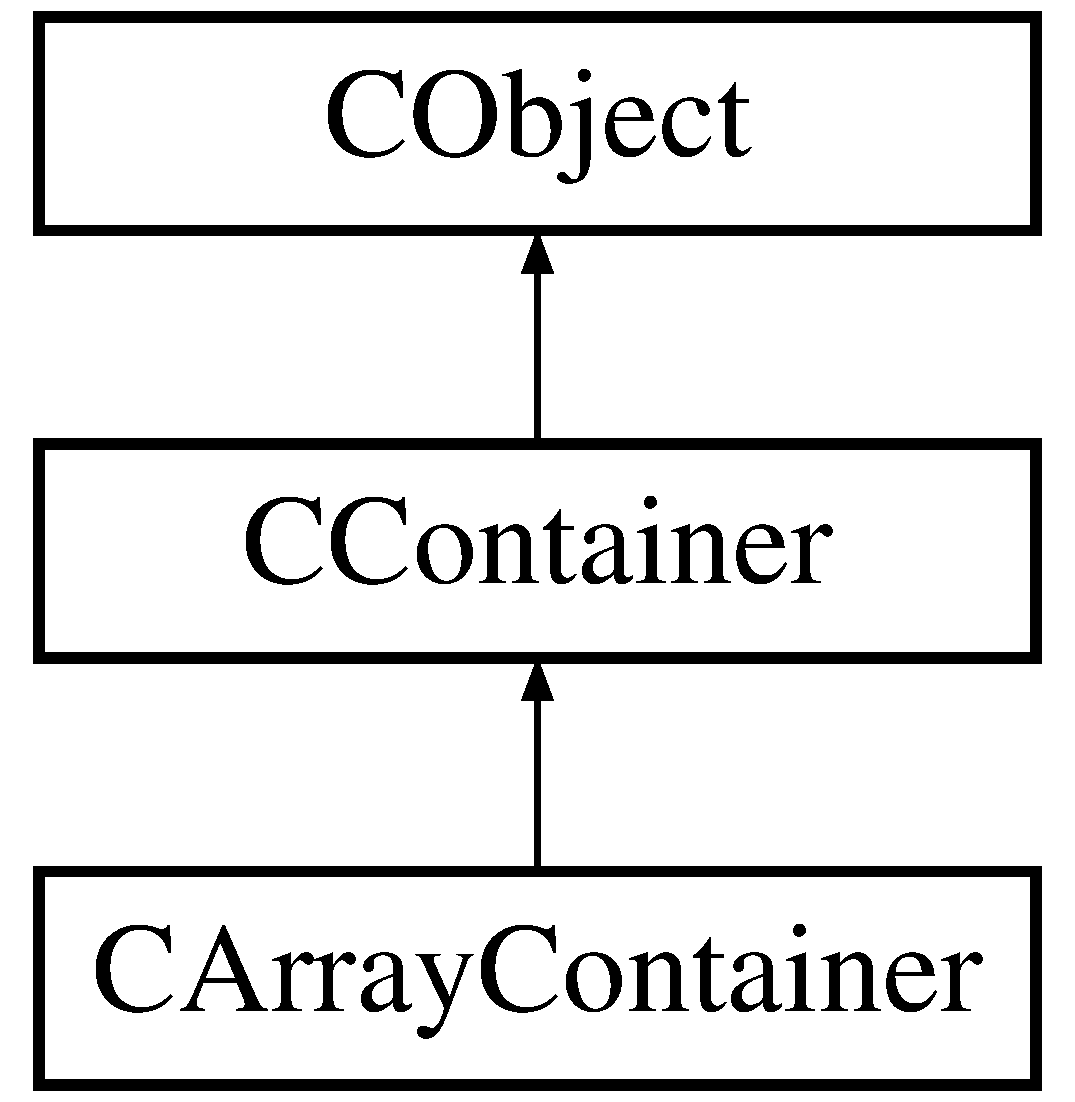
\includegraphics[height=3.000000cm]{class_c_array_container}
\end{center}
\end{figure}
\subsection*{Public Member Functions}
\begin{DoxyCompactItemize}
\item 
\hyperlink{class_c_array_container_a10e83176c2a2ee0d9fe53ca9e51b0ca0}{\-\_\-\-\_\-construct} (\$the\-Container=N\-U\-L\-L)
\item 
\hyperlink{class_c_array_container_ac63eeb55a8c374668c5c443fb6e27df3}{Container} (\$the\-Value=N\-U\-L\-L, \$get\-Old=F\-A\-L\-S\-E)
\item 
\hyperlink{class_c_array_container_ac89f1c53cc6680107cfb4703bd5103ca}{Commit} (\&\$the\-Object, \$the\-Identifier=N\-U\-L\-L, \$the\-Modifiers=k\-F\-L\-A\-G\-\_\-\-P\-E\-R\-S\-I\-S\-T\-\_\-\-R\-E\-P\-L\-A\-C\-E)
\end{DoxyCompactItemize}
\subsection*{Protected Member Functions}
\begin{DoxyCompactItemize}
\item 
\hyperlink{class_c_array_container_aed066fb29aae224fe77ce3d6e4540cac}{\-\_\-\-Commit} (\&\$the\-Object, \$the\-Identifier, \$the\-Modifiers)
\item 
\hyperlink{class_c_array_container_ac970cd81e09a1b87c6cad960de74856d}{\-\_\-\-Load} (\$the\-Identifier, \$the\-Modifiers)
\item 
\hyperlink{class_c_array_container_a7a6026166105a3d9281c3556836844bc}{\-\_\-\-Delete} (\$the\-Identifier, \$the\-Modifiers)
\end{DoxyCompactItemize}


\subsection{Constructor \& Destructor Documentation}
\hypertarget{class_c_array_container_a10e83176c2a2ee0d9fe53ca9e51b0ca0}{\index{C\-Array\-Container@{C\-Array\-Container}!\-\_\-\-\_\-construct@{\-\_\-\-\_\-construct}}
\index{\-\_\-\-\_\-construct@{\-\_\-\-\_\-construct}!CArrayContainer@{C\-Array\-Container}}
\subsubsection[{\-\_\-\-\_\-construct}]{\setlength{\rightskip}{0pt plus 5cm}{\bf C\-Array\-Container\-::\-\_\-\-\_\-construct} (
\begin{DoxyParamCaption}
\item[{\$}]{the\-Container = {\ttfamily NULL}}
\end{DoxyParamCaption}
)}}\label{class_c_array_container_a10e83176c2a2ee0d9fe53ca9e51b0ca0}
Instantiate class.

We \hyperlink{class_c_container_af2fc42b4d7b5f71e0f127c941440b1aa}{overload} this method to provide a default native container, which, in this case, will be an empty array.


\begin{DoxyParams}[1]{Parameters}
mixed & {\em \$the\-Container} & Native persistent container.\\
\hline
\end{DoxyParams}
public 

Reimplemented from \hyperlink{class_c_container_af2fc42b4d7b5f71e0f127c941440b1aa}{C\-Container}.



\subsection{Member Function Documentation}
\hypertarget{class_c_array_container_aed066fb29aae224fe77ce3d6e4540cac}{\index{C\-Array\-Container@{C\-Array\-Container}!\-\_\-\-Commit@{\-\_\-\-Commit}}
\index{\-\_\-\-Commit@{\-\_\-\-Commit}!CArrayContainer@{C\-Array\-Container}}
\subsubsection[{\-\_\-\-Commit}]{\setlength{\rightskip}{0pt plus 5cm}{\bf C\-Array\-Container\-::\-\_\-\-Commit} (
\begin{DoxyParamCaption}
\item[{\&\$}]{the\-Object, }
\item[{\$}]{the\-Identifier, }
\item[{\$}]{the\-Modifiers}
\end{DoxyParamCaption}
)\hspace{0.3cm}{\ttfamily  \mbox{[}protected\mbox{]}}}}\label{class_c_array_container_aed066fb29aae224fe77ce3d6e4540cac}
Commit provided object.

We implement this method to handle array or Array\-Object stores and we ensure provided options are followed.

By default the object must be an array or Array\-Object, any other type will raise an \hyperlink{}{exception}.

The provided identifier will be cast to a string. If it is {\itshape N\-U\-L\-L\/}, it means that the object is to be appended in the container and the method assumes the \hyperlink{class_c_array_container_ac89f1c53cc6680107cfb4703bd5103ca}{caller} has determined that it is an \hyperlink{}{insert} operation.

Although the \hyperlink{class_c_array_container_ac89f1c53cc6680107cfb4703bd5103ca}{caller} accepts the \hyperlink{}{delete} option, in this class we do not, so we shall raise an \hyperlink{}{exception}.


\begin{DoxyParams}[1]{Parameters}
reference & {\em \&\$the\-Object} & Object to commit. \\
\hline
mixed & {\em \$the\-Identifier} & Object identifier. \\
\hline
bitfield & {\em \$the\-Modifiers} & Commit modifiers.\\
\hline
\end{DoxyParams}
protected \begin{DoxyReturn}{Returns}
mixed 
\end{DoxyReturn}


Reimplemented from \hyperlink{class_c_container_a95c13ac30a01bd5ee684fe1baf0d8d43}{C\-Container}.

\hypertarget{class_c_array_container_a7a6026166105a3d9281c3556836844bc}{\index{C\-Array\-Container@{C\-Array\-Container}!\-\_\-\-Delete@{\-\_\-\-Delete}}
\index{\-\_\-\-Delete@{\-\_\-\-Delete}!CArrayContainer@{C\-Array\-Container}}
\subsubsection[{\-\_\-\-Delete}]{\setlength{\rightskip}{0pt plus 5cm}{\bf C\-Array\-Container\-::\-\_\-\-Delete} (
\begin{DoxyParamCaption}
\item[{\$}]{the\-Identifier, }
\item[{\$}]{the\-Modifiers}
\end{DoxyParamCaption}
)\hspace{0.3cm}{\ttfamily  \mbox{[}protected\mbox{]}}}}\label{class_c_array_container_a7a6026166105a3d9281c3556836844bc}
Delete object.

We implement this method to handle array or Array\-Object stores.

The method will cast the identifier to a string.


\begin{DoxyParams}[1]{Parameters}
mixed & {\em \$the\-Identifier} & Object identifier. \\
\hline
bitfield & {\em \$the\-Modifiers} & Load modifiers.\\
\hline
\end{DoxyParams}
protected \begin{DoxyReturn}{Returns}
mixed 
\end{DoxyReturn}


Reimplemented from \hyperlink{class_c_container_adb859efe2ce642d29d3bff48a806789d}{C\-Container}.

\hypertarget{class_c_array_container_ac970cd81e09a1b87c6cad960de74856d}{\index{C\-Array\-Container@{C\-Array\-Container}!\-\_\-\-Load@{\-\_\-\-Load}}
\index{\-\_\-\-Load@{\-\_\-\-Load}!CArrayContainer@{C\-Array\-Container}}
\subsubsection[{\-\_\-\-Load}]{\setlength{\rightskip}{0pt plus 5cm}{\bf C\-Array\-Container\-::\-\_\-\-Load} (
\begin{DoxyParamCaption}
\item[{\$}]{the\-Identifier, }
\item[{\$}]{the\-Modifiers}
\end{DoxyParamCaption}
)\hspace{0.3cm}{\ttfamily  \mbox{[}protected\mbox{]}}}}\label{class_c_array_container_ac970cd81e09a1b87c6cad960de74856d}
Load object.

We implement this method to handle array or Array\-Object stores.

The method will cast the identifier to a string.


\begin{DoxyParams}[1]{Parameters}
mixed & {\em \$the\-Identifier} & Object identifier. \\
\hline
bitfield & {\em \$the\-Modifiers} & Load modifiers.\\
\hline
\end{DoxyParams}
protected \begin{DoxyReturn}{Returns}
mixed 
\end{DoxyReturn}


Reimplemented from \hyperlink{class_c_container_a93d34640379c1debc9542609bf4b34e9}{C\-Container}.

\hypertarget{class_c_array_container_ac89f1c53cc6680107cfb4703bd5103ca}{\index{C\-Array\-Container@{C\-Array\-Container}!Commit@{Commit}}
\index{Commit@{Commit}!CArrayContainer@{C\-Array\-Container}}
\subsubsection[{Commit}]{\setlength{\rightskip}{0pt plus 5cm}{\bf C\-Array\-Container\-::\-Commit} (
\begin{DoxyParamCaption}
\item[{\&\$}]{the\-Object, }
\item[{\$}]{the\-Identifier = {\ttfamily NULL}, }
\item[{\$}]{the\-Modifiers = {\ttfamily kFLAG\-\_\-PERSIST\-\_\-REPLACE}}
\end{DoxyParamCaption}
)}}\label{class_c_array_container_ac89f1c53cc6680107cfb4703bd5103ca}
Commit provided object.

We \hyperlink{class_c_container_a4847dc676d1f7704e75f8981e927508a}{overload} this method to check whether the provided object is either an array or an Array\-Object.


\begin{DoxyParams}[1]{Parameters}
reference & {\em \&\$the\-Object} & Object to commit. \\
\hline
mixed & {\em \$the\-Identifier} & Object identifier. \\
\hline
bitfield & {\em \$the\-Modifiers} & Commit modifiers.\\
\hline
\end{DoxyParams}
public \begin{DoxyReturn}{Returns}
mixed 
\end{DoxyReturn}


Reimplemented from \hyperlink{class_c_container_a4847dc676d1f7704e75f8981e927508a}{C\-Container}.

\hypertarget{class_c_array_container_ac63eeb55a8c374668c5c443fb6e27df3}{\index{C\-Array\-Container@{C\-Array\-Container}!Container@{Container}}
\index{Container@{Container}!CArrayContainer@{C\-Array\-Container}}
\subsubsection[{Container}]{\setlength{\rightskip}{0pt plus 5cm}{\bf C\-Array\-Container\-::\-Container} (
\begin{DoxyParamCaption}
\item[{\$}]{the\-Value = {\ttfamily NULL}, }
\item[{\$}]{get\-Old = {\ttfamily FALSE}}
\end{DoxyParamCaption}
)}}\label{class_c_array_container_ac63eeb55a8c374668c5c443fb6e27df3}
Manage persistent container.

We \hyperlink{class_c_container_a7d10fa70dfa381cb95e66c265e2ca113}{overload} this method to ensure that the provided container is either an array or an Array\-Object.


\begin{DoxyParams}[1]{Parameters}
mixed & {\em \$the\-Value} & Persistent container or operation. \\
\hline
boolean & {\em \$get\-Old} & T\-R\-U\-E get old value.\\
\hline
\end{DoxyParams}
public \begin{DoxyReturn}{Returns}
mixed
\end{DoxyReturn}
\hyperlink{class_c_object_a9b8dccdadcf4fea58f915bd9b228e23e}{Manage\-Member()} 

Reimplemented from \hyperlink{class_c_container_a7d10fa70dfa381cb95e66c265e2ca113}{C\-Container}.



The documentation for this class was generated from the following file\-:\begin{DoxyCompactItemize}
\item 
/\-Library/\-Web\-Server/\-Library/wrapper/classes/C\-Array\-Container.\-php\end{DoxyCompactItemize}

\hypertarget{class_c_array_object}{\section{C\-Array\-Object Class Reference}
\label{class_c_array_object}\index{C\-Array\-Object@{C\-Array\-Object}}
}
Inheritance diagram for C\-Array\-Object\-:\begin{figure}[H]
\begin{center}
\leavevmode
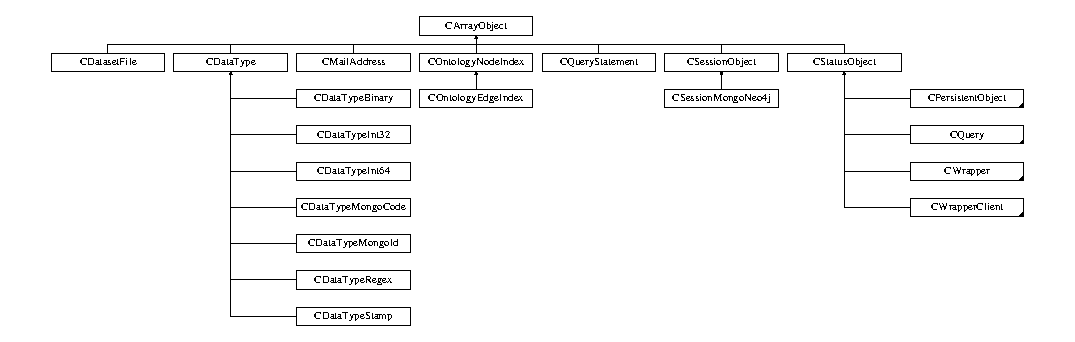
\includegraphics[height=5.874125cm]{class_c_array_object}
\end{center}
\end{figure}
\subsection*{Public Member Functions}
\begin{DoxyCompactItemize}
\item 
\hyperlink{class_c_array_object_ac9929feeb67c76a0e055696abffe2fb6}{offset\-Get} (\$the\-Offset)
\item 
\hyperlink{class_c_array_object_a41815b543b14d373f68ed34ca53dc9f6}{offset\-Set} (\$the\-Offset, \$the\-Value)
\item 
\hyperlink{class_c_array_object_a2852b78f58379e507b5e7d7cb8e5326b}{offset\-Unset} (\$the\-Offset)
\item 
\hyperlink{class_c_array_object_a350d95184af98e75868f27ea170270ce}{keys} ()
\item 
\hyperlink{class_c_array_object_a1f29fcc343a624354f6096fd6a4621e6}{values} ()
\end{DoxyCompactItemize}
\subsection*{Protected Member Functions}
\begin{DoxyCompactItemize}
\item 
\hyperlink{class_c_array_object_a931cb8b30569b811a18adc0161eb3603}{\-\_\-\-Manage\-Offset} (\$the\-Offset, \$the\-Value=N\-U\-L\-L, \$get\-Old=F\-A\-L\-S\-E)
\item 
\hyperlink{class_c_array_object_a056b7a3218ffb9a2eb992c029124a669}{\-\_\-\-Manage\-Array\-Offset} (\$the\-Offset, \$the\-Value=N\-U\-L\-L, \$the\-Operation=N\-U\-L\-L, \$get\-Old=F\-A\-L\-S\-E)
\item 
\hyperlink{class_c_array_object_af714f81bb75f725c6868fb286c59b160}{\-\_\-\-Manage\-Typed\-Array\-Offset} (\$the\-Offset, \$the\-Type=N\-U\-L\-L, \$the\-Data=N\-U\-L\-L, \$get\-Old=F\-A\-L\-S\-E)
\end{DoxyCompactItemize}


\subsection{Member Function Documentation}
\hypertarget{class_c_array_object_a056b7a3218ffb9a2eb992c029124a669}{\index{C\-Array\-Object@{C\-Array\-Object}!\-\_\-\-Manage\-Array\-Offset@{\-\_\-\-Manage\-Array\-Offset}}
\index{\-\_\-\-Manage\-Array\-Offset@{\-\_\-\-Manage\-Array\-Offset}!CArrayObject@{C\-Array\-Object}}
\subsubsection[{\-\_\-\-Manage\-Array\-Offset}]{\setlength{\rightskip}{0pt plus 5cm}{\bf C\-Array\-Object\-::\-\_\-\-Manage\-Array\-Offset} (
\begin{DoxyParamCaption}
\item[{\$}]{the\-Offset, }
\item[{\$}]{the\-Value = {\ttfamily NULL}, }
\item[{\$}]{the\-Operation = {\ttfamily NULL}, }
\item[{\$}]{get\-Old = {\ttfamily FALSE}}
\end{DoxyParamCaption}
)\hspace{0.3cm}{\ttfamily  \mbox{[}protected\mbox{]}}}}\label{class_c_array_object_a056b7a3218ffb9a2eb992c029124a669}
Manage an array offset.

This library implements a standard interface for managing object properties using methods, this method extends the approach to offset members that are in the form of arrays, in which it should be possible to cast the values to strings and these strings should be unique within the list\-:


\begin{DoxyItemize}
\item {\bfseries \$the\-Offset}\-: The offset to manage. 
\item {\bfseries \$the\-Value}\-: This parameter represents either the value to add, or the index of the element to operate on\-: 
\begin{DoxyItemize}
\item {\itshape N\-U\-L\-L\/}\-: This value indicates that we want to operate on all elements, which means that we are either retrieving the full list or deleting it. 
\item {\itshape array\/}\-: This value indicates that we want to replace the whole list, this will only be tested if the next parameter evaluates to {\itshape T\-R\-U\-E\/}. 
\item {\itshape other\/}\-: Any other type represents either the new value to be added or the index to the value to be returned or deleted. {\itshape It must be possible to cast this value to a string, this is what will be used to compare elements\/}. 
\end{DoxyItemize}
\item {\bfseries \$the\-Operation}\-: This parameter represents the operation to be performed, it will be evaluated as a boolean and its scope depends on the value of the previous parameter\-: 
\begin{DoxyItemize}
\item {\itshape N\-U\-L\-L\/}\-: Return the element or list. 
\item {\itshape F\-A\-L\-S\-E\/}\-: Delete the element or list. 
\item {\itshape T\-R\-U\-E\/}\-: Add the element or list. Note that with this value, if you provide {\itshape N\-U\-L\-L\/} in the previous parameter, it will be equivalent to deleting the whole list. 
\end{DoxyItemize}
\item {\bfseries \$get\-Old}\-: Determines what the method will return\-: 
\begin{DoxyItemize}
\item {\itshape T\-R\-U\-E\/}\-: Return the element or list {\itshape before\/} it was eventually modified. 
\item {\itshape F\-A\-L\-S\-E\/}\-: Return the element or list {\itshape after\/} it was eventually modified. 
\end{DoxyItemize}
\end{DoxyItemize}


\begin{DoxyParams}[1]{Parameters}
string & {\em \$the\-Offset} & Offset. \\
\hline
mixed & {\em \$the\-Value} & Value or index. \\
\hline
mixed & {\em \$the\-Operation} & Operation. \\
\hline
boolean & {\em \$get\-Old} & T\-R\-U\-E get old value.\\
\hline
\end{DoxyParams}
protected \begin{DoxyReturn}{Returns}
mixed
\end{DoxyReturn}
\hyperlink{class_c_array_object_ac9929feeb67c76a0e055696abffe2fb6}{offset\-Get()}  \hyperlink{class_c_array_object_a41815b543b14d373f68ed34ca53dc9f6}{offset\-Set()}  \hyperlink{class_c_array_object_a2852b78f58379e507b5e7d7cb8e5326b}{offset\-Unset()} \hypertarget{class_c_array_object_a931cb8b30569b811a18adc0161eb3603}{\index{C\-Array\-Object@{C\-Array\-Object}!\-\_\-\-Manage\-Offset@{\-\_\-\-Manage\-Offset}}
\index{\-\_\-\-Manage\-Offset@{\-\_\-\-Manage\-Offset}!CArrayObject@{C\-Array\-Object}}
\subsubsection[{\-\_\-\-Manage\-Offset}]{\setlength{\rightskip}{0pt plus 5cm}{\bf C\-Array\-Object\-::\-\_\-\-Manage\-Offset} (
\begin{DoxyParamCaption}
\item[{\$}]{the\-Offset, }
\item[{\$}]{the\-Value = {\ttfamily NULL}, }
\item[{\$}]{get\-Old = {\ttfamily FALSE}}
\end{DoxyParamCaption}
)\hspace{0.3cm}{\ttfamily  \mbox{[}protected\mbox{]}}}}\label{class_c_array_object_a931cb8b30569b811a18adc0161eb3603}
Manage an offset.

This library implements a standard interface for managing object properties using methods, this method extends the approach to offset members\-:


\begin{DoxyItemize}
\item {\bfseries \$the\-Offset}\-: The offset to manage. 
\item {\bfseries \$the\-Value}\-: The value or operation\-: 
\begin{DoxyItemize}
\item {\itshape N\-U\-L\-L\/}\-: Return the offset's current value. 
\item {\itshape F\-A\-L\-S\-E\/}\-: Delete the offset. 
\item {\itshape other\/}\-: Any other type represents the offset's new value. 
\end{DoxyItemize}
\item {\bfseries \$get\-Old}\-: Determines what the method will return\-: 
\begin{DoxyItemize}
\item {\itshape T\-R\-U\-E\/}\-: Return the value of the offset {\itshape before\/} it was eventually modified. 
\item {\itshape F\-A\-L\-S\-E\/}\-: Return the value of the offset {\itshape after\/} it was eventually modified. 
\end{DoxyItemize}
\end{DoxyItemize}


\begin{DoxyParams}[1]{Parameters}
string & {\em \$the\-Offset} & Offset. \\
\hline
mixed & {\em \$the\-Value} & Value or operation. \\
\hline
boolean & {\em \$get\-Old} & T\-R\-U\-E get old value.\\
\hline
\end{DoxyParams}
protected \begin{DoxyReturn}{Returns}
mixed
\end{DoxyReturn}
\hyperlink{class_c_array_object_ac9929feeb67c76a0e055696abffe2fb6}{offset\-Get()}  \hyperlink{class_c_array_object_a41815b543b14d373f68ed34ca53dc9f6}{offset\-Set()}  \hyperlink{class_c_array_object_a2852b78f58379e507b5e7d7cb8e5326b}{offset\-Unset()} \hypertarget{class_c_array_object_af714f81bb75f725c6868fb286c59b160}{\index{C\-Array\-Object@{C\-Array\-Object}!\-\_\-\-Manage\-Typed\-Array\-Offset@{\-\_\-\-Manage\-Typed\-Array\-Offset}}
\index{\-\_\-\-Manage\-Typed\-Array\-Offset@{\-\_\-\-Manage\-Typed\-Array\-Offset}!CArrayObject@{C\-Array\-Object}}
\subsubsection[{\-\_\-\-Manage\-Typed\-Array\-Offset}]{\setlength{\rightskip}{0pt plus 5cm}{\bf C\-Array\-Object\-::\-\_\-\-Manage\-Typed\-Array\-Offset} (
\begin{DoxyParamCaption}
\item[{\$}]{the\-Offset, }
\item[{\$}]{the\-Type = {\ttfamily NULL}, }
\item[{\$}]{the\-Data = {\ttfamily NULL}, }
\item[{\$}]{get\-Old = {\ttfamily FALSE}}
\end{DoxyParamCaption}
)\hspace{0.3cm}{\ttfamily  \mbox{[}protected\mbox{]}}}}\label{class_c_array_object_af714f81bb75f725c6868fb286c59b160}
Manage a typed array offset.

This library implements a standard interface for managing object properties using methods, this method extends the approach to offset members that are in the form of arrays, in which each element is itself an array of two items\-:


\begin{DoxyItemize}
\item {\itshape \hyperlink{}{k\-T\-A\-G\-\_\-\-T\-Y\-P\-E}\/}\-: This element represents the qualifier of the item, it provides a type or qualification for the next element. It must be possible to cast this value to a string. 
\item {\itshape \hyperlink{}{k\-T\-A\-G\-\_\-\-D\-A\-T\-A}\/}\-: This element represents the element data. 
\end{DoxyItemize}

No two elements of the list can share the same \hyperlink{}{type}. You may have one element without \hyperlink{}{type}, this one may be considered the default element.

This method is intended for managing list elements rather than the list itself, for the latter purpose use the offset management methods.

The parameters to this method are\-:


\begin{DoxyItemize}
\item {\bfseries \$the\-Offset}\-: The offset to manage. 
\item {\bfseries \$the\-Type}\-: This parameter represents the value of the \hyperlink{}{type} element of the item, depending on the next parameter this value will be used for matching items in the list\-: 
\begin{DoxyItemize}
\item {\itshape N\-U\-L\-L\/}\-: An empty type means that we are looking for the item lacking the \hyperlink{}{k\-T\-A\-G\-\_\-\-T\-Y\-P\-E} tag. 
\item {\itshape array\/}\-: If you provide an array, it means that you are operating on a list of items\-: depending on the next parameter this will mean either retrieving the \hyperlink{}{data} elements of the items matching the array, deleting these items, or adding/replacing the items; in this last case, this means that the next parameter must also be an array and that each of its elements will be associated to the corresponding \hyperlink{}{type} element. 
\item {\itshape other\/}\-: Any other value will be considered as the type to retrieve, remove or add/replace. You {\itshape M\-U\-S\-T\/} be able to cast this value to a string. 
\end{DoxyItemize}
\item {\bfseries \$the\-Data}\-: This parameter represents the item's \hyperlink{}{data} element, or the operation to be performed\-: 
\begin{DoxyItemize}
\item {\itshape N\-U\-L\-L\/}\-: This indicates that we want to retrieve the data of the item with \hyperlink{}{type} matching the previous parameter. 
\item {\itshape F\-A\-L\-S\-E\/}\-: This indicates that we want to remove the item matching the \hyperlink{}{type} provided in the previous parameter. 
\item {\itshape other\/}\-: Any other value indicates that we want to add or replace the \hyperlink{}{data} element of the item matching the previous parameter. Note that if the previous parameter is an array, this one must also be an array matching the latter's count. 
\end{DoxyItemize}
\item {\bfseries \$get\-Old}\-: Determines what the method will return\-: 
\begin{DoxyItemize}
\item {\itshape T\-R\-U\-E\/}\-: Return the element or list {\itshape before\/} it was eventually modified. 
\item {\itshape F\-A\-L\-S\-E\/}\-: Return the element or list {\itshape after\/} it was eventually modified. 
\end{DoxyItemize}
\end{DoxyItemize}


\begin{DoxyParams}[1]{Parameters}
string & {\em \$the\-Offset} & Offset. \\
\hline
mixed & {\em \$the\-Type} & Element type. \\
\hline
mixed & {\em \$the\-Data} & Element value. \\
\hline
boolean & {\em \$get\-Old} & T\-R\-U\-E get old value.\\
\hline
\end{DoxyParams}
protected \begin{DoxyReturn}{Returns}
mixed
\end{DoxyReturn}
\hyperlink{class_c_array_object_ac9929feeb67c76a0e055696abffe2fb6}{offset\-Get()}  \hyperlink{class_c_array_object_a41815b543b14d373f68ed34ca53dc9f6}{offset\-Set()}  \hyperlink{class_c_array_object_a2852b78f58379e507b5e7d7cb8e5326b}{offset\-Unset()} \hypertarget{class_c_array_object_a350d95184af98e75868f27ea170270ce}{\index{C\-Array\-Object@{C\-Array\-Object}!keys@{keys}}
\index{keys@{keys}!CArrayObject@{C\-Array\-Object}}
\subsubsection[{keys}]{\setlength{\rightskip}{0pt plus 5cm}{\bf C\-Array\-Object\-::keys} (
\begin{DoxyParamCaption}
{}
\end{DoxyParamCaption}
)}}\label{class_c_array_object_a350d95184af98e75868f27ea170270ce}
Return object's keys.

This method has the same function as array's {\itshape array\-\_\-keys()\/}, it will return an array comprised of all object's offsets.

public \begin{DoxyReturn}{Returns}
array 
\end{DoxyReturn}
\hypertarget{class_c_array_object_ac9929feeb67c76a0e055696abffe2fb6}{\index{C\-Array\-Object@{C\-Array\-Object}!offset\-Get@{offset\-Get}}
\index{offset\-Get@{offset\-Get}!CArrayObject@{C\-Array\-Object}}
\subsubsection[{offset\-Get}]{\setlength{\rightskip}{0pt plus 5cm}{\bf C\-Array\-Object\-::offset\-Get} (
\begin{DoxyParamCaption}
\item[{\$}]{the\-Offset}
\end{DoxyParamCaption}
)}}\label{class_c_array_object_ac9929feeb67c76a0e055696abffe2fb6}
Return a value at a given offset.

This method should return the value corresponding to the provided offset.

This method is overloaded to prevent notices from being triggered when seeking non-\/existing offsets.

In this class no offset may have a {\itshape N\-U\-L\-L\/} value, if this method returns a {\itshape N\-U\-L\-L\/} value, it means that the offset doesn't exist.


\begin{DoxyParams}[1]{Parameters}
string & {\em \$the\-Offset} & Offset.\\
\hline
\end{DoxyParams}
public \begin{DoxyReturn}{Returns}
mixed 
\end{DoxyReturn}
\hypertarget{class_c_array_object_a41815b543b14d373f68ed34ca53dc9f6}{\index{C\-Array\-Object@{C\-Array\-Object}!offset\-Set@{offset\-Set}}
\index{offset\-Set@{offset\-Set}!CArrayObject@{C\-Array\-Object}}
\subsubsection[{offset\-Set}]{\setlength{\rightskip}{0pt plus 5cm}{\bf C\-Array\-Object\-::offset\-Set} (
\begin{DoxyParamCaption}
\item[{\$}]{the\-Offset, }
\item[{\$}]{the\-Value}
\end{DoxyParamCaption}
)}}\label{class_c_array_object_a41815b543b14d373f68ed34ca53dc9f6}
Set a value for a given offset.

This method should set the provided value corresponding to the provided offset.

This method is overloaded to prevent setting {\itshape N\-U\-L\-L\/} values\-: if this is the case, the method will \hyperlink{class_c_array_object_a2852b78f58379e507b5e7d7cb8e5326b}{delete} the offset.


\begin{DoxyParams}[1]{Parameters}
string & {\em \$the\-Offset} & Offset. \\
\hline
string | N\-U\-L\-L & {\em \$the\-Value} & Value to set at offset.\\
\hline
\end{DoxyParams}
public

\hyperlink{class_c_array_object_a2852b78f58379e507b5e7d7cb8e5326b}{offset\-Unset()} 

Reimplemented in \hyperlink{class_c_entity_a193cf3d19057021bb6e779644730eac8}{C\-Entity}, \hyperlink{class_c_user_aace3446b9cacfe28cc1937c608fcc999}{C\-User}, and \hyperlink{class_c_status_object_a140ef140d4fa1c4a6180e843bd5ec969}{C\-Status\-Object}.

\hypertarget{class_c_array_object_a2852b78f58379e507b5e7d7cb8e5326b}{\index{C\-Array\-Object@{C\-Array\-Object}!offset\-Unset@{offset\-Unset}}
\index{offset\-Unset@{offset\-Unset}!CArrayObject@{C\-Array\-Object}}
\subsubsection[{offset\-Unset}]{\setlength{\rightskip}{0pt plus 5cm}{\bf C\-Array\-Object\-::offset\-Unset} (
\begin{DoxyParamCaption}
\item[{\$}]{the\-Offset}
\end{DoxyParamCaption}
)}}\label{class_c_array_object_a2852b78f58379e507b5e7d7cb8e5326b}
Reset a value for a given offset.

This method should reset the value corresponding to the provided offset.

We overload this method to prevent notices on non-\/existing offsets.


\begin{DoxyParams}[1]{Parameters}
string & {\em \$the\-Offset} & Offset.\\
\hline
\end{DoxyParams}
public 

Reimplemented in \hyperlink{class_c_entity_a887a87fc716e36a0d4c1477dbaf5bb67}{C\-Entity}, \hyperlink{class_c_user_aed8557e18a89d868cedf5a48328b33b2}{C\-User}, and \hyperlink{class_c_status_object_ae733db1bbfffcbe894ea405765ab4150}{C\-Status\-Object}.

\hypertarget{class_c_array_object_a1f29fcc343a624354f6096fd6a4621e6}{\index{C\-Array\-Object@{C\-Array\-Object}!values@{values}}
\index{values@{values}!CArrayObject@{C\-Array\-Object}}
\subsubsection[{values}]{\setlength{\rightskip}{0pt plus 5cm}{\bf C\-Array\-Object\-::values} (
\begin{DoxyParamCaption}
{}
\end{DoxyParamCaption}
)}}\label{class_c_array_object_a1f29fcc343a624354f6096fd6a4621e6}
Return object's values.

This method has the same function as array's {\itshape array\-\_\-values()\/}, it will return an array comprised of all object's values.

public \begin{DoxyReturn}{Returns}
array 
\end{DoxyReturn}


The documentation for this class was generated from the following file\-:\begin{DoxyCompactItemize}
\item 
/\-Library/\-Web\-Server/\-Library/wrapper/classes/C\-Array\-Object.\-php\end{DoxyCompactItemize}

\hypertarget{class_c_attribute}{\section{C\-Attribute Class Reference}
\label{class_c_attribute}\index{C\-Attribute@{C\-Attribute}}
}
\subsection*{Static Public Member Functions}
\begin{DoxyCompactItemize}
\item 
static \hyperlink{class_c_attribute_a9d231a47718719fcd6c33f3d0ac91675}{Manage\-Offset} (\&\$the\-Reference, \$the\-Offset, \$the\-Value=N\-U\-L\-L, \$get\-Old=F\-A\-L\-S\-E)
\item 
static \hyperlink{class_c_attribute_a7d2e35b120eaa55529f78253f77dab48}{Manage\-Array\-Offset} (\&\$the\-Reference, \$the\-Offset, \$the\-Value=N\-U\-L\-L, \$the\-Operation=N\-U\-L\-L, \$get\-Old=F\-A\-L\-S\-E)
\item 
static \hyperlink{class_c_attribute_af163f41d2a8e052c09afe094195ca007}{Manage\-Typed\-Offset} (\&\$the\-Reference, \$the\-Main\-Offset, \$the\-Type\-Offset, \$the\-Data\-Offset, \$the\-Type=N\-U\-L\-L, \$the\-Data=N\-U\-L\-L, \$get\-Old=F\-A\-L\-S\-E)
\item 
static \hyperlink{class_c_attribute_a9841820c02fde7e8f0b9c0a31b8ab1fa}{Manage\-Typed\-Array\-Offset} (\&\$the\-Reference, \$the\-Main\-Offset, \$the\-Type\-Offset, \$the\-Data\-Offset, \$the\-Type, \$the\-Data=N\-U\-L\-L, \$the\-Operation=N\-U\-L\-L, \$get\-Old=F\-A\-L\-S\-E)
\item 
static \hyperlink{class_c_attribute_ab0b7e532b3e0b4dca8fbab9b522e5332}{Manage\-Typed\-Kind\-Offset} (\&\$the\-Reference, \$the\-Main\-Offset, \$the\-Kind\-Offset, \$the\-Type\-Offset, \$the\-Data\-Offset, \$the\-Kind, \$the\-Type, \$the\-Data=N\-U\-L\-L, \$get\-Old=F\-A\-L\-S\-E)
\item 
static \hyperlink{class_c_attribute_a58d5de30d4a6ea29f485a266460a2bdd}{Manage\-Object\-List} (\&\$the\-Reference, \$the\-Main\-Offset, \$the\-Type\-Offset, \$the\-Data\-Offset, \$the\-Value, \$the\-Operation=N\-U\-L\-L, \$get\-Old=F\-A\-L\-S\-E)
\end{DoxyCompactItemize}


\subsection{Member Function Documentation}
\hypertarget{class_c_attribute_a7d2e35b120eaa55529f78253f77dab48}{\index{C\-Attribute@{C\-Attribute}!Manage\-Array\-Offset@{Manage\-Array\-Offset}}
\index{Manage\-Array\-Offset@{Manage\-Array\-Offset}!CAttribute@{C\-Attribute}}
\subsubsection[{Manage\-Array\-Offset}]{\setlength{\rightskip}{0pt plus 5cm}static C\-Attribute\-::\-Manage\-Array\-Offset (
\begin{DoxyParamCaption}
\item[{\&}]{\$the\-Reference, }
\item[{}]{\$the\-Offset, }
\item[{}]{\$the\-Value = {\ttfamily NULL}, }
\item[{}]{\$the\-Operation = {\ttfamily NULL}, }
\item[{}]{\$get\-Old = {\ttfamily FALSE}}
\end{DoxyParamCaption}
)\hspace{0.3cm}{\ttfamily [static]}}}\label{class_c_attribute_a7d2e35b120eaa55529f78253f77dab48}
Manage an array offset.

This method can be used to manage an array offset, this options involves setting, retrieving and deleting elements of an offset which contains an array of values, this method concentrates in managing the offset's elements, rather than \hyperlink{class_c_attribute_a9d231a47718719fcd6c33f3d0ac91675}{managing} the offset itself.

The offset's array should be composed by elements that {\itshape must} be convertable to strings\-: the string value represents the index of the element, which means that no two elements can have the same string value.

When deleting elements, if the list becomes empty, the whole offset will be deleted.

The method accepts the following parameters\-:


\begin{DoxyItemize}
\item {\bfseries \&\$the\-Reference}\-: Reference to an array or Array\-Object derived instance. 
\item {\bfseries \$the\-Offset}\-: The offset to manage. 
\item {\bfseries \$the\-Value}\-: This parameter represents the data element to be set, or the index to the data element to be deleted or retrieved\-: 
\begin{DoxyItemize}
\item {\itshape N\-U\-L\-L}\-: This value indicates that we want to operate on all elements, which means, depending on the next parameter, that we are either retrieving or deleting the full list. If the operation parameter is {\itshape T\-R\-U\-E}, no element will be added. 
\item {\itshape array}\-: This value indicates that we want to operate on a list of values\-: each of these values will be handled according to the operation parameter. Note that an Array\-Object is not considered in this scenario, so in that case you would have to convert it to an array. 
\item {\itshape other}\-: Any other type represents either the new value to be added or the index to the value to be returned or deleted. {\itshape It must be possible to cast this value to a string, this is what will be used to compare elements}. 
\end{DoxyItemize}
\item {\bfseries \$the\-Operation}\-: This parameter represents the operation to be performed, it will be evaluated as a boolean and its scope depends on the value of the previous parameter\-: 
\begin{DoxyItemize}
\item {\itshape N\-U\-L\-L}\-: Return the element or list. 
\item {\itshape F\-A\-L\-S\-E}\-: Delete the element or list. 
\item {\itshape T\-R\-U\-E}\-: Add the element or list. If you provided {\itshape N\-U\-L\-L} as value, the operation will do nothing. 
\end{DoxyItemize}
\item {\bfseries \$get\-Old}\-: Determines what the method will return\-: 
\begin{DoxyItemize}
\item {\itshape T\-R\-U\-E}\-: Return the value {\itshape before} it was eventually modified. 
\item {\itshape F\-A\-L\-S\-E}\-: Return the value {\itshape after} it was eventually modified. 
\end{DoxyItemize}
\end{DoxyItemize}


\begin{DoxyParams}[1]{Parameters}
reference & {\em \&\$the\-Reference} & Object reference. \\
\hline
string & {\em \$the\-Offset} & Offset. \\
\hline
mixed & {\em \$the\-Value} & Value to manage. \\
\hline
mixed & {\em \$the\-Operation} & Operation to perform. \\
\hline
boolean & {\em \$get\-Old} & T\-R\-U\-E get old value.\\
\hline
\end{DoxyParams}
\begin{DoxyReturn}{Returns}
mixed 
\end{DoxyReturn}
\hypertarget{class_c_attribute_a58d5de30d4a6ea29f485a266460a2bdd}{\index{C\-Attribute@{C\-Attribute}!Manage\-Object\-List@{Manage\-Object\-List}}
\index{Manage\-Object\-List@{Manage\-Object\-List}!CAttribute@{C\-Attribute}}
\subsubsection[{Manage\-Object\-List}]{\setlength{\rightskip}{0pt plus 5cm}static C\-Attribute\-::\-Manage\-Object\-List (
\begin{DoxyParamCaption}
\item[{\&}]{\$the\-Reference, }
\item[{}]{\$the\-Main\-Offset, }
\item[{}]{\$the\-Type\-Offset, }
\item[{}]{\$the\-Data\-Offset, }
\item[{}]{\$the\-Value, }
\item[{}]{\$the\-Operation = {\ttfamily NULL}, }
\item[{}]{\$get\-Old = {\ttfamily FALSE}}
\end{DoxyParamCaption}
)\hspace{0.3cm}{\ttfamily [static]}}}\label{class_c_attribute_a58d5de30d4a6ea29f485a266460a2bdd}
Manage a list of object references.

This method can be used to manage a list of object references, in which each element is either\-:


\begin{DoxyItemize}
\item {\itshape Scalar}\-: A scalar or object representing\-: 
\begin{DoxyItemize}
\item {\itshape The object}\-: The actual referenced object. 
\item {\itshape The object reference}\-: An object reference structure or a scalar representing the object \hyperlink{}{identifier}. 
\end{DoxyItemize}or\-: 
\item {\itshape Array}\-: A structure composed of two items\-: 
\begin{DoxyItemize}
\item {\itshape Kind}\-: This offset represents the type or predicate of the reference. 
\item {\itshape Data}\-: This offset represents the actual object or object reference. 
\end{DoxyItemize}
\end{DoxyItemize}

The reference list is numerically indexed array and this method will ensure it remains so.

The method accepts the following parameters\-:


\begin{DoxyItemize}
\item {\bfseries \&\$the\-Reference}\-: Reference to an array or Array\-Object derived instance. 
\item {\bfseries \$the\-Main\-Offset}\-: The offset to manage. 
\item {\bfseries \$the\-Type\-Offset}\-: The element's offset of the type or predicate. 
\item {\bfseries \$the\-Data\-Offset}\-: The element's offset of the data. 
\item {\bfseries \$the\-Value}\-: This parameter represents either the search key in the list when retrieving or deleting, or the reference when replacing or adding. If you provide an array, it means that the elements may have a kind offset and that the reference or object must be found in the data offset. When matching, if the kind offset is not provided, it means that only those elements that do not have a kind offset will be selected for matching. If the types match, the method will use the \hyperlink{class_c_persistent_unit_object_ac7bfe8f6475e61abb2e9de9c112cbfe6}{Object\-Identifier} method to match the references, please refer to its documentation for more information. If the provided value is not an array, it means that the reference list does not feature types, so matches will only be performed on the reference. 
\item {\bfseries \$the\-Operation}\-: The operation to perform\-: 
\begin{DoxyItemize}
\item {\itshape N\-U\-L\-L}\-: Return the element matched by the previous parameter. 
\item {\itshape F\-A\-L\-S\-E}\-: Delete the element matched by the previous parameter and return it. 
\item {\itshape other}\-: Any other value means that we want to add to the list the element provided in the previous parameter, either appending it if there was no matching element, or by replacing a matching element. The method will return either the replaced element or the new one. 
\end{DoxyItemize}
\item {\bfseries \$get\-Old}\-: Determines what the method will return when deleting or replacing\-: 
\begin{DoxyItemize}
\item {\itshape T\-R\-U\-E}\-: Return the deleted or replaced element. 
\item {\itshape F\-A\-L\-S\-E}\-: Return the replacing element or {\itshape N\-U\-L\-L} when deleting. 
\end{DoxyItemize}
\end{DoxyItemize}

The \hyperlink{class_c_persistent_unit_object_ac7bfe8f6475e61abb2e9de9c112cbfe6}{method} used to match the list elements expects \hyperlink{}{identifiers} in the references or objects, if these are not there, there is no way to discern duplicates.


\begin{DoxyParams}[1]{Parameters}
reference & {\em \&\$the\-Reference} & Object reference. \\
\hline
string & {\em \$the\-Main\-Offset} & Main offset. \\
\hline
string & {\em \$the\-Type\-Offset} & Type offset. \\
\hline
string & {\em \$the\-Data\-Offset} & Data offset. \\
\hline
mixed & {\em \$the\-Value} & Reference or instance. \\
\hline
mixed & {\em \$the\-Operation} & Operation. \\
\hline
boolean & {\em \$get\-Old} & T\-R\-U\-E get old value.\\
\hline
\end{DoxyParams}
protected \begin{DoxyReturn}{Returns}
mixed 
\end{DoxyReturn}
\hypertarget{class_c_attribute_a9d231a47718719fcd6c33f3d0ac91675}{\index{C\-Attribute@{C\-Attribute}!Manage\-Offset@{Manage\-Offset}}
\index{Manage\-Offset@{Manage\-Offset}!CAttribute@{C\-Attribute}}
\subsubsection[{Manage\-Offset}]{\setlength{\rightskip}{0pt plus 5cm}static C\-Attribute\-::\-Manage\-Offset (
\begin{DoxyParamCaption}
\item[{\&}]{\$the\-Reference, }
\item[{}]{\$the\-Offset, }
\item[{}]{\$the\-Value = {\ttfamily NULL}, }
\item[{}]{\$get\-Old = {\ttfamily FALSE}}
\end{DoxyParamCaption}
)\hspace{0.3cm}{\ttfamily [static]}}}\label{class_c_attribute_a9d231a47718719fcd6c33f3d0ac91675}
Manage a scalar offset.

This method can be used to manage a scalar offset, this options involves setting, retrieving and deleting an offset of the provided array or Array\-Object.

The method accepts the following parameters\-:


\begin{DoxyItemize}
\item {\bfseries \&\$the\-Reference}\-: Reference to an array or Array\-Object derived instance. 
\item {\bfseries \$the\-Offset}\-: The offset to manage. 
\item {\bfseries \$the\-Value}\-: The value or operation\-: 
\begin{DoxyItemize}
\item {\itshape N\-U\-L\-L}\-: Return the offset's current value. 
\item {\itshape F\-A\-L\-S\-E}\-: Delete the offset. 
\item {\itshape other}\-: Any other type represents the offset's new value. 
\end{DoxyItemize}
\item {\bfseries \$get\-Old}\-: Determines what the method will return\-: 
\begin{DoxyItemize}
\item {\itshape T\-R\-U\-E}\-: Return the value of the offset {\itshape before} it was eventually modified. 
\item {\itshape F\-A\-L\-S\-E}\-: Return the value of the offset {\itshape after} it was eventually modified. 
\end{DoxyItemize}
\end{DoxyItemize}


\begin{DoxyParams}[1]{Parameters}
reference & {\em \&\$the\-Reference} & Object reference. \\
\hline
string & {\em \$the\-Offset} & Offset. \\
\hline
mixed & {\em \$the\-Value} & Value or operation. \\
\hline
boolean & {\em \$get\-Old} & T\-R\-U\-E get old value.\\
\hline
\end{DoxyParams}
\begin{DoxyReturn}{Returns}
mixed 
\end{DoxyReturn}
\hypertarget{class_c_attribute_a9841820c02fde7e8f0b9c0a31b8ab1fa}{\index{C\-Attribute@{C\-Attribute}!Manage\-Typed\-Array\-Offset@{Manage\-Typed\-Array\-Offset}}
\index{Manage\-Typed\-Array\-Offset@{Manage\-Typed\-Array\-Offset}!CAttribute@{C\-Attribute}}
\subsubsection[{Manage\-Typed\-Array\-Offset}]{\setlength{\rightskip}{0pt plus 5cm}static C\-Attribute\-::\-Manage\-Typed\-Array\-Offset (
\begin{DoxyParamCaption}
\item[{\&}]{\$the\-Reference, }
\item[{}]{\$the\-Main\-Offset, }
\item[{}]{\$the\-Type\-Offset, }
\item[{}]{\$the\-Data\-Offset, }
\item[{}]{\$the\-Type, }
\item[{}]{\$the\-Data = {\ttfamily NULL}, }
\item[{}]{\$the\-Operation = {\ttfamily NULL}, }
\item[{}]{\$get\-Old = {\ttfamily FALSE}}
\end{DoxyParamCaption}
)\hspace{0.3cm}{\ttfamily [static]}}}\label{class_c_attribute_a9841820c02fde7e8f0b9c0a31b8ab1fa}
Manage a typed array offset.

A typed array offset is structured as follows\-:


\begin{DoxyItemize}
\item {\itshape Type}\-: This offset contains a scalar which determined the type or category of the element. This offset may be omitted. 
\item {\itshape Data}\-: This offset contains the element data as an array of data elements, these elements are handled by the \hyperlink{class_c_attribute_a7d2e35b120eaa55529f78253f77dab48}{Manage\-Array\-Offset} method. 
\end{DoxyItemize}

No two elements may share the same type or category and all data elements within a category must be unique.

The method accepts the following parameters\-:


\begin{DoxyItemize}
\item {\bfseries \&\$the\-Reference}\-: Reference to an array or Array\-Object derived instance. 
\item {\bfseries \$the\-Main\-Offset}\-: The offset to manage. 
\item {\bfseries \$the\-Type\-Offset}\-: The element's offset of the type or category. 
\item {\bfseries \$the\-Data\-Offset}\-: The element's offset of the data. 
\item {\bfseries \$the\-Type}\-: This parameter represents the index to the offset's elements. 
\item {\bfseries \$the\-Data}\-: This parameter represents the element's data element, if {\itshape N\-U\-L\-L} or omitted, it implieas that the operation applies to the whole list of data elements. 
\item {\bfseries \$the\-Operation}\-: This parameter represents the operation to be performed, it will be evaluated as a boolean and its scope depends on the value of the previous parameter\-: 
\begin{DoxyItemize}
\item {\itshape N\-U\-L\-L}\-: Return the element or list. 
\item {\itshape F\-A\-L\-S\-E}\-: Delete the element or list. 
\item {\itshape T\-R\-U\-E}\-: Add the element or list. 
\end{DoxyItemize}
\item {\bfseries \$get\-Old}\-: Determines what the method will return\-: 
\begin{DoxyItemize}
\item {\itshape T\-R\-U\-E}\-: Return the value of the offset {\itshape before} it was eventually modified. 
\item {\itshape F\-A\-L\-S\-E}\-: Return the value of the offset {\itshape after} it was eventually modified. 
\end{DoxyItemize}
\end{DoxyItemize}

The method will return the matched element's value of the data offset.


\begin{DoxyParams}[1]{Parameters}
reference & {\em \&\$the\-Reference} & Object reference. \\
\hline
string & {\em \$the\-Main\-Offset} & Main offset. \\
\hline
string & {\em \$the\-Type\-Offset} & Type offset. \\
\hline
string & {\em \$the\-Data\-Offset} & Data offset. \\
\hline
mixed & {\em \$the\-Type} & Type. \\
\hline
mixed & {\em \$the\-Data} & Data or operation. \\
\hline
mixed & {\em \$the\-Operation} & Operation to perform. \\
\hline
boolean & {\em \$get\-Old} & T\-R\-U\-E get old value.\\
\hline
\end{DoxyParams}
\begin{DoxyReturn}{Returns}
mixed 
\end{DoxyReturn}
\hypertarget{class_c_attribute_ab0b7e532b3e0b4dca8fbab9b522e5332}{\index{C\-Attribute@{C\-Attribute}!Manage\-Typed\-Kind\-Offset@{Manage\-Typed\-Kind\-Offset}}
\index{Manage\-Typed\-Kind\-Offset@{Manage\-Typed\-Kind\-Offset}!CAttribute@{C\-Attribute}}
\subsubsection[{Manage\-Typed\-Kind\-Offset}]{\setlength{\rightskip}{0pt plus 5cm}static C\-Attribute\-::\-Manage\-Typed\-Kind\-Offset (
\begin{DoxyParamCaption}
\item[{\&}]{\$the\-Reference, }
\item[{}]{\$the\-Main\-Offset, }
\item[{}]{\$the\-Kind\-Offset, }
\item[{}]{\$the\-Type\-Offset, }
\item[{}]{\$the\-Data\-Offset, }
\item[{}]{\$the\-Kind, }
\item[{}]{\$the\-Type, }
\item[{}]{\$the\-Data = {\ttfamily NULL}, }
\item[{}]{\$get\-Old = {\ttfamily FALSE}}
\end{DoxyParamCaption}
)\hspace{0.3cm}{\ttfamily [static]}}}\label{class_c_attribute_ab0b7e532b3e0b4dca8fbab9b522e5332}
Manage a category and type offset.

A typed kind offset is structured as follows\-:


\begin{DoxyItemize}
\item {\itshape Kind}\-: This offset contains a scalar which determined the kind or category of the element, this element may be omitted. 
\item {\itshape Type}\-: This element represents the type of the next item, this element is required. 
\item {\itshape Data}\-: This offset contains the element data, in this method we treat it as a scalar, this element is required. 
\end{DoxyItemize}

No two elements of the list can share the same kind and type, these represent the index of the array.

The parameters to this method are\-:


\begin{DoxyItemize}
\item {\bfseries \&\$the\-Reference}\-: Reference to an array or Array\-Object derived instance. 
\item {\bfseries \$the\-Main\-Offset}\-: The offset to manage. 
\item {\bfseries \$the\-Kind\-Offset}\-: The element's offset of the kind. 
\item {\bfseries \$the\-Type\-Offset}\-: The element's offset of the type. 
\item {\bfseries \$the\-Data\-Offset}\-: The element's offset of the data. 
\item {\bfseries \$the\-Kind}\-: The item kind value; this value may be {\itshape N\-U\-L\-L}, or one should be able to cast it to a string. 
\item {\bfseries \$the\-Type}\-: The item type value; one should be able to cast the value to a string. 
\item {\bfseries \$the\-Data}\-: This parameter represents the item's data element, or the operation to be performed\-: 
\begin{DoxyItemize}
\item {\itshape N\-U\-L\-L}\-: This indicates that we want to retrieve the data of the item with index matching the kind and type parameters. 
\item {\itshape F\-A\-L\-S\-E}\-: This indicates that we want to remove the item matching the kind and type parameters. 
\item {\itshape other}\-: Any other value indicates that we want to add or replace the data element of the item matching the kind and type parameters. 
\end{DoxyItemize}
\item {\bfseries \$get\-Old}\-: Determines what the method will return\-: 
\begin{DoxyItemize}
\item {\itshape T\-R\-U\-E}\-: Return the element or list {\itshape before} it was eventually modified. 
\item {\itshape F\-A\-L\-S\-E}\-: Return the element or list {\itshape after} it was eventually modified. 
\end{DoxyItemize}
\end{DoxyItemize}


\begin{DoxyParams}[1]{Parameters}
reference & {\em \&\$the\-Reference} & Object reference. \\
\hline
string & {\em \$the\-Main\-Offset} & Main offset. \\
\hline
string & {\em \$the\-Kind\-Offset} & Type offset. \\
\hline
string & {\em \$the\-Type\-Offset} & Type offset. \\
\hline
string & {\em \$the\-Data\-Offset} & Data offset. \\
\hline
mixed & {\em \$the\-Kind} & Item kind. \\
\hline
mixed & {\em \$the\-Type} & Item type. \\
\hline
mixed & {\em \$the\-Data} & Item value. \\
\hline
boolean & {\em \$get\-Old} & T\-R\-U\-E get old value.\\
\hline
\end{DoxyParams}
\begin{DoxyReturn}{Returns}
mixed
\end{DoxyReturn}
offset\-Get()  offset\-Set()  offset\-Unset() \hypertarget{class_c_attribute_af163f41d2a8e052c09afe094195ca007}{\index{C\-Attribute@{C\-Attribute}!Manage\-Typed\-Offset@{Manage\-Typed\-Offset}}
\index{Manage\-Typed\-Offset@{Manage\-Typed\-Offset}!CAttribute@{C\-Attribute}}
\subsubsection[{Manage\-Typed\-Offset}]{\setlength{\rightskip}{0pt plus 5cm}static C\-Attribute\-::\-Manage\-Typed\-Offset (
\begin{DoxyParamCaption}
\item[{\&}]{\$the\-Reference, }
\item[{}]{\$the\-Main\-Offset, }
\item[{}]{\$the\-Type\-Offset, }
\item[{}]{\$the\-Data\-Offset, }
\item[{}]{\$the\-Type = {\ttfamily NULL}, }
\item[{}]{\$the\-Data = {\ttfamily NULL}, }
\item[{}]{\$get\-Old = {\ttfamily FALSE}}
\end{DoxyParamCaption}
)\hspace{0.3cm}{\ttfamily [static]}}}\label{class_c_attribute_af163f41d2a8e052c09afe094195ca007}
Manage a typed offset.

A typed offset is structured as follows\-:


\begin{DoxyItemize}
\item {\itshape Type}\-: This offset contains a scalar which determined the type or category of the element. This offset may be omitted. 
\item {\itshape Data}\-: This offset contains the element data, in this method we treat it as a scalar. This offset may not be omitted. 
\end{DoxyItemize}

No two elements may share the same type or category.

The method accepts the following parameters\-:


\begin{DoxyItemize}
\item {\bfseries \&\$the\-Reference}\-: Reference to an array or Array\-Object derived instance. 
\item {\bfseries \$the\-Main\-Offset}\-: The offset to manage. 
\item {\bfseries \$the\-Type\-Offset}\-: The element's offset of the type or category. 
\item {\bfseries \$the\-Data\-Offset}\-: The element's offset of the data. 
\item {\bfseries \$the\-Type}\-: This parameter represents the value of the index element of the item, depending on the next parameter this value will be used for matching items in the list\-: 
\begin{DoxyItemize}
\item {\itshape N\-U\-L\-L}\-: An empty type means that we are looking for the item lacking the index element. 
\item {\itshape array}\-: If you provide an array, it means that you are operating on a list of items\-: depending on the next parameter this will mean either retrieving the data elements of the items matching the array, deleting these items, or adding/replacing the items; in this lastcase, this means that the next parameter must also be an array and that each of its elements will be associated to the corresponding index element. 
\item {\itshape other}\-: Any other value will be considered as the index to retrieve, remove or add/replace. You {\itshape M\-U\-S\-T} be able to cast this value to a string. 
\end{DoxyItemize}
\item {\bfseries \$the\-Data}\-: This parameter represents the item's data element, or the operation to be performed\-: 
\begin{DoxyItemize}
\item {\itshape N\-U\-L\-L}\-: This indicates that we want to retrieve the data of the item with index matching the previous parameter. 
\item {\itshape F\-A\-L\-S\-E}\-: This indicates that we want to remove the item matching the index provided in the previous parameter. 
\item {\itshape other}\-: Any other value indicates that we want to add or replace the data element of the item matching the previous parameter. Note that if the previous parameter is an array, this one must also be an array matching the latter's count. 
\end{DoxyItemize}
\item {\bfseries \$get\-Old}\-: Determines what the method will return\-: 
\begin{DoxyItemize}
\item {\itshape T\-R\-U\-E}\-: Return the value of the offset {\itshape before} it was eventually modified. 
\item {\itshape F\-A\-L\-S\-E}\-: Return the value of the offset {\itshape after} it was eventually modified. 
\end{DoxyItemize}
\end{DoxyItemize}

The method will return the matched element's value of the data offset.


\begin{DoxyParams}[1]{Parameters}
reference & {\em \&\$the\-Reference} & Object reference. \\
\hline
string & {\em \$the\-Main\-Offset} & Main offset. \\
\hline
string & {\em \$the\-Type\-Offset} & Type offset. \\
\hline
string & {\em \$the\-Data\-Offset} & Data offset. \\
\hline
mixed & {\em \$the\-Type} & Type. \\
\hline
mixed & {\em \$the\-Data} & Data or operation. \\
\hline
boolean & {\em \$get\-Old} & T\-R\-U\-E get old value.\\
\hline
\end{DoxyParams}
\begin{DoxyReturn}{Returns}
mixed 
\end{DoxyReturn}


The documentation for this class was generated from the following file\-:\begin{DoxyCompactItemize}
\item 
/\-Library/\-Web\-Server/\-Library/wrapper/classes/C\-Attribute.\-php\end{DoxyCompactItemize}

\hypertarget{class_c_coded_unit_object}{\section{C\-Coded\-Unit\-Object Class Reference}
\label{class_c_coded_unit_object}\index{C\-Coded\-Unit\-Object@{C\-Coded\-Unit\-Object}}
}
Inheritance diagram for C\-Coded\-Unit\-Object\-:\begin{figure}[H]
\begin{center}
\leavevmode
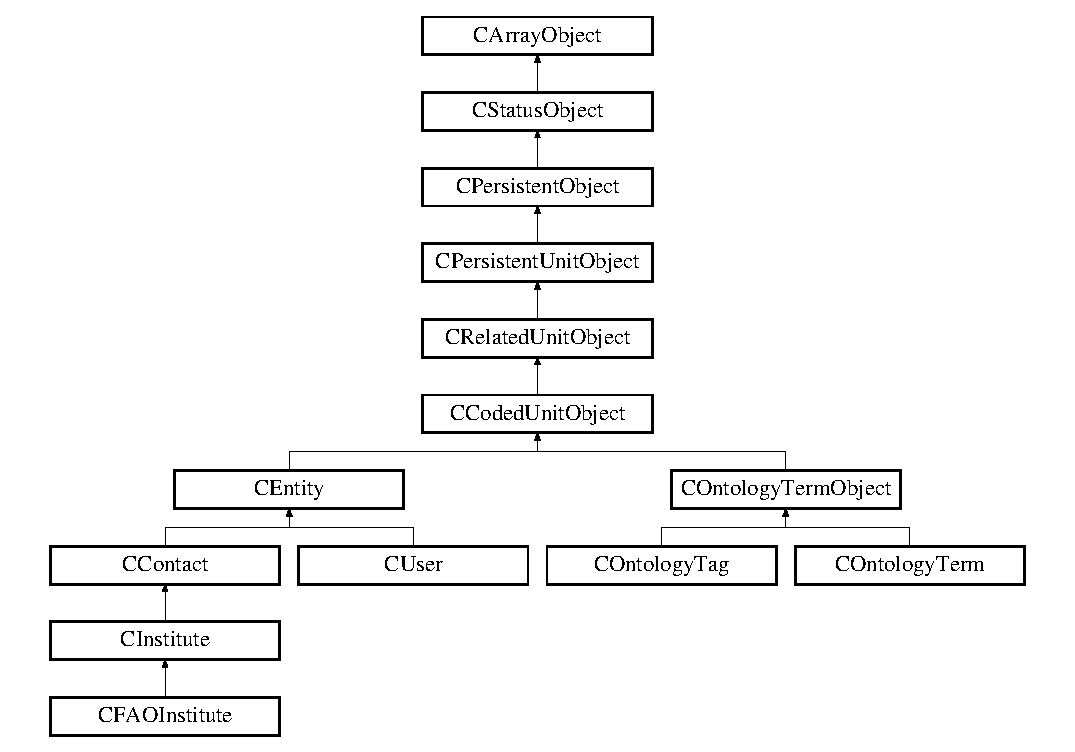
\includegraphics[height=10.000000cm]{class_c_coded_unit_object}
\end{center}
\end{figure}
\subsection*{Public Member Functions}
\begin{DoxyCompactItemize}
\item 
\hyperlink{class_c_coded_unit_object_a314fc62af62314f5ac5acca2ac809900}{\-\_\-\-\_\-construct} (\$the\-Container=N\-U\-L\-L, \$the\-Identifier=N\-U\-L\-L, \$the\-Modifiers=k\-F\-L\-A\-G\-\_\-\-D\-E\-F\-A\-U\-L\-T)
\item 
\hyperlink{class_c_coded_unit_object_a56af949800e65f9a283239d2e455259f}{Code} (\$the\-Value=N\-U\-L\-L, \$get\-Old=F\-A\-L\-S\-E)
\item 
\hyperlink{class_c_coded_unit_object_aafe9f12551f9f183c21a9865f0e9c670}{Kind} (\$the\-Value=N\-U\-L\-L, \$the\-Operation=N\-U\-L\-L, \$get\-Old=F\-A\-L\-S\-E)
\item 
\hyperlink{class_c_coded_unit_object_a6cbad4f609a1a247dcd955d588750668}{Created} (\$the\-Value=N\-U\-L\-L, \$get\-Old=F\-A\-L\-S\-E)
\item 
\hyperlink{class_c_coded_unit_object_a0943e9d09e1078908938970b02a4b586}{Modified} (\$the\-Value=N\-U\-L\-L, \$get\-Old=F\-A\-L\-S\-E)
\item 
\hyperlink{class_c_coded_unit_object_a49bb8f2956cb0551ba827b222778f295}{offset\-Set} (\$the\-Offset, \$the\-Value)
\item 
\hyperlink{class_c_coded_unit_object_a5072e0f72c19260df212a4cf93c9f1cb}{offset\-Unset} (\$the\-Offset)
\end{DoxyCompactItemize}
\subsection*{Protected Member Functions}
\begin{DoxyCompactItemize}
\item 
\hyperlink{class_c_coded_unit_object_a990c19b8bf98d2784da81e3a3121ce56}{\-\_\-index} ()
\end{DoxyCompactItemize}
\subsection*{Additional Inherited Members}


\subsection{Constructor \& Destructor Documentation}
\hypertarget{class_c_coded_unit_object_a314fc62af62314f5ac5acca2ac809900}{\index{C\-Coded\-Unit\-Object@{C\-Coded\-Unit\-Object}!\-\_\-\-\_\-construct@{\-\_\-\-\_\-construct}}
\index{\-\_\-\-\_\-construct@{\-\_\-\-\_\-construct}!CCodedUnitObject@{C\-Coded\-Unit\-Object}}
\subsubsection[{\-\_\-\-\_\-construct}]{\setlength{\rightskip}{0pt plus 5cm}C\-Coded\-Unit\-Object\-::\-\_\-\-\_\-construct (
\begin{DoxyParamCaption}
\item[{}]{\$the\-Container = {\ttfamily NULL}, }
\item[{}]{\$the\-Identifier = {\ttfamily NULL}, }
\item[{}]{\$the\-Modifiers = {\ttfamily kFLAG\-\_\-DEFAULT}}
\end{DoxyParamCaption}
)}}\label{class_c_coded_unit_object_a314fc62af62314f5ac5acca2ac809900}
Instantiate class.

We \hyperlink{class_c_persistent_object_a0f0729cfaef48bd1c98c0711c061a7d3}{overload} the constructor to initialise the \hyperlink{class_c_status_object_a8429102e4f52f7558649b64f4e673a69}{inited} \hyperlink{}{flag} if the \hyperlink{class_c_coded_unit_object_a56af949800e65f9a283239d2e455259f}{code} attribute is set.


\begin{DoxyParams}[1]{Parameters}
mixed & {\em \$the\-Container} & Persistent container. \\
\hline
mixed & {\em \$the\-Identifier} & Object identifier. \\
\hline
bitfield & {\em \$the\-Modifiers} & Create modifiers.\\
\hline
\end{DoxyParams}
public

\-\_\-\-Is\-Inited

\begin{DoxySeeAlso}{See also}
k\-T\-A\-G\-\_\-\-C\-O\-D\-E 
\end{DoxySeeAlso}


Reimplemented from \hyperlink{class_c_persistent_object_a0f0729cfaef48bd1c98c0711c061a7d3}{C\-Persistent\-Object}.



Reimplemented in \hyperlink{class_c_user_af83ffccb40893a43d90eafe396cbdec1}{C\-User}, \hyperlink{class_c_institute_a468ba723fabd5a67bea5016d1531b147}{C\-Institute}, \hyperlink{class_c_ontology_term_a33679101b2a63044f0084918a8df123e}{C\-Ontology\-Term}, and \hyperlink{class_c_ontology_term_object_af1fb502088538ad7372719c20f73bc5c}{C\-Ontology\-Term\-Object}.



\subsection{Member Function Documentation}
\hypertarget{class_c_coded_unit_object_a990c19b8bf98d2784da81e3a3121ce56}{\index{C\-Coded\-Unit\-Object@{C\-Coded\-Unit\-Object}!\-\_\-index@{\-\_\-index}}
\index{\-\_\-index@{\-\_\-index}!CCodedUnitObject@{C\-Coded\-Unit\-Object}}
\subsubsection[{\-\_\-index}]{\setlength{\rightskip}{0pt plus 5cm}C\-Coded\-Unit\-Object\-::\-\_\-index (
\begin{DoxyParamCaption}
{}
\end{DoxyParamCaption}
)\hspace{0.3cm}{\ttfamily [protected]}}}\label{class_c_coded_unit_object_a990c19b8bf98d2784da81e3a3121ce56}
Return the object's unique index.

In this class we consider the \hyperlink{}{code} to be the object's unique \hyperlink{}{identifier}.

protected \begin{DoxyReturn}{Returns}
string 
\end{DoxyReturn}


Reimplemented from \hyperlink{class_c_persistent_unit_object_a5166fdce0b1be6a3e4889f20c5f1c2dd}{C\-Persistent\-Unit\-Object}.



Reimplemented in \hyperlink{class_c_term_a7524effdc0db8f5ca045f306e3b6b50e}{C\-Term}.

\hypertarget{class_c_coded_unit_object_a56af949800e65f9a283239d2e455259f}{\index{C\-Coded\-Unit\-Object@{C\-Coded\-Unit\-Object}!Code@{Code}}
\index{Code@{Code}!CCodedUnitObject@{C\-Coded\-Unit\-Object}}
\subsubsection[{Code}]{\setlength{\rightskip}{0pt plus 5cm}C\-Coded\-Unit\-Object\-::\-Code (
\begin{DoxyParamCaption}
\item[{}]{\$the\-Value = {\ttfamily NULL}, }
\item[{}]{\$get\-Old = {\ttfamily FALSE}}
\end{DoxyParamCaption}
)}}\label{class_c_coded_unit_object_a56af949800e65f9a283239d2e455259f}
Manage code.

This method can be used to handle the object's \hyperlink{}{code}, it uses the standard accessor \hyperlink{class_c_attribute_a9d231a47718719fcd6c33f3d0ac91675}{method} to manage the \hyperlink{}{offset}.

The code represents the object's \hyperlink{class_c_coded_unit_object_a990c19b8bf98d2784da81e3a3121ce56}{identifier}.

For a more in-\/depth reference of this method, please consult the \hyperlink{class_c_attribute_a9d231a47718719fcd6c33f3d0ac91675}{Manage\-Offset} method, in which the first parameter will be the constant \hyperlink{}{k\-T\-A\-G\-\_\-\-C\-O\-D\-E}.


\begin{DoxyParams}[1]{Parameters}
mixed & {\em \$the\-Value} & Value. \\
\hline
boolean & {\em \$get\-Old} & T\-R\-U\-E get old value.\\
\hline
\end{DoxyParams}
public \begin{DoxyReturn}{Returns}
string
\end{DoxyReturn}
\hyperlink{class_c_attribute_a9d231a47718719fcd6c33f3d0ac91675}{C\-Attribute\-::\-Manage\-Offset()}

\begin{DoxySeeAlso}{See also}
k\-T\-A\-G\-\_\-\-C\-O\-D\-E 
\end{DoxySeeAlso}
\hypertarget{class_c_coded_unit_object_a6cbad4f609a1a247dcd955d588750668}{\index{C\-Coded\-Unit\-Object@{C\-Coded\-Unit\-Object}!Created@{Created}}
\index{Created@{Created}!CCodedUnitObject@{C\-Coded\-Unit\-Object}}
\subsubsection[{Created}]{\setlength{\rightskip}{0pt plus 5cm}C\-Coded\-Unit\-Object\-::\-Created (
\begin{DoxyParamCaption}
\item[{}]{\$the\-Value = {\ttfamily NULL}, }
\item[{}]{\$get\-Old = {\ttfamily FALSE}}
\end{DoxyParamCaption}
)}}\label{class_c_coded_unit_object_a6cbad4f609a1a247dcd955d588750668}
Manage object creation time stamp.

This method can be used to manage the object \hyperlink{}{creation} time-\/stamp, it uses the standard accessor \hyperlink{class_c_attribute_a9d231a47718719fcd6c33f3d0ac91675}{method} to manage the \hyperlink{}{offset}\-:


\begin{DoxyItemize}
\item {\bfseries \$the\-Value}\-: The value or operation\-: 
\begin{DoxyItemize}
\item {\itshape N\-U\-L\-L}\-: Return the current value. 
\item {\itshape F\-A\-L\-S\-E}\-: Delete the value. 
\item {\itshape other}\-: Set value. 
\end{DoxyItemize}
\item {\bfseries \$get\-Old}\-: Determines what the method will return\-: 
\begin{DoxyItemize}
\item {\itshape T\-R\-U\-E}\-: Return the value {\itshape before} it was eventually modified. 
\item {\itshape F\-A\-L\-S\-E}\-: Return the value {\itshape after} it was eventually modified. 
\end{DoxyItemize}
\end{DoxyItemize}


\begin{DoxyParams}[1]{Parameters}
N\-U\-L\-L | F\-A\-L\-S\-E | string & {\em \$the\-Value} & Object creation date. \\
\hline
boolean & {\em \$get\-Old} & T\-R\-U\-E get old value.\\
\hline
\end{DoxyParams}
public \begin{DoxyReturn}{Returns}
string
\end{DoxyReturn}
\hyperlink{class_c_attribute_a9d231a47718719fcd6c33f3d0ac91675}{C\-Attribute\-::\-Manage\-Offset()}

\begin{DoxySeeAlso}{See also}
k\-T\-A\-G\-\_\-\-C\-R\-E\-A\-T\-E\-D 
\end{DoxySeeAlso}
\hypertarget{class_c_coded_unit_object_aafe9f12551f9f183c21a9865f0e9c670}{\index{C\-Coded\-Unit\-Object@{C\-Coded\-Unit\-Object}!Kind@{Kind}}
\index{Kind@{Kind}!CCodedUnitObject@{C\-Coded\-Unit\-Object}}
\subsubsection[{Kind}]{\setlength{\rightskip}{0pt plus 5cm}C\-Coded\-Unit\-Object\-::\-Kind (
\begin{DoxyParamCaption}
\item[{}]{\$the\-Value = {\ttfamily NULL}, }
\item[{}]{\$the\-Operation = {\ttfamily NULL}, }
\item[{}]{\$get\-Old = {\ttfamily FALSE}}
\end{DoxyParamCaption}
)}}\label{class_c_coded_unit_object_aafe9f12551f9f183c21a9865f0e9c670}
Manage kind.

This method can be used to handle the object's \hyperlink{}{kinds}, it uses the standard accessor \hyperlink{class_c_attribute_a7d2e35b120eaa55529f78253f77dab48}{method} to manage the list of kinds.

Each element of this list should indicate a function or quality of the current object

For a more thorough reference of how this method works, please consult the \hyperlink{class_c_attribute_a7d2e35b120eaa55529f78253f77dab48}{C\-Attribute\-::\-Manage\-Array\-Offset} method, in which the second parameter will be the constant \hyperlink{}{k\-T\-A\-G\-\_\-\-K\-I\-N\-D}.


\begin{DoxyParams}[1]{Parameters}
mixed & {\em \$the\-Value} & Value or index. \\
\hline
mixed & {\em \$the\-Operation} & Operation. \\
\hline
boolean & {\em \$get\-Old} & T\-R\-U\-E get old value.\\
\hline
\end{DoxyParams}
public \begin{DoxyReturn}{Returns}
mixed
\end{DoxyReturn}
\hyperlink{class_c_attribute_a7d2e35b120eaa55529f78253f77dab48}{C\-Attribute\-::\-Manage\-Array\-Offset()}

\begin{DoxySeeAlso}{See also}
k\-T\-A\-G\-\_\-\-K\-I\-N\-D 
\end{DoxySeeAlso}
\hypertarget{class_c_coded_unit_object_a0943e9d09e1078908938970b02a4b586}{\index{C\-Coded\-Unit\-Object@{C\-Coded\-Unit\-Object}!Modified@{Modified}}
\index{Modified@{Modified}!CCodedUnitObject@{C\-Coded\-Unit\-Object}}
\subsubsection[{Modified}]{\setlength{\rightskip}{0pt plus 5cm}C\-Coded\-Unit\-Object\-::\-Modified (
\begin{DoxyParamCaption}
\item[{}]{\$the\-Value = {\ttfamily NULL}, }
\item[{}]{\$get\-Old = {\ttfamily FALSE}}
\end{DoxyParamCaption}
)}}\label{class_c_coded_unit_object_a0943e9d09e1078908938970b02a4b586}
Manage object last modification time stamp.

This method can be used to manage the object last \hyperlink{}{modification} time-\/stamp, or the date in which the last modification was made on the object, it uses the standard accessor \hyperlink{class_c_attribute_a9d231a47718719fcd6c33f3d0ac91675}{method} to manage the \hyperlink{}{offset}\-:


\begin{DoxyItemize}
\item {\bfseries \$the\-Value}\-: The value or operation\-: 
\begin{DoxyItemize}
\item {\itshape N\-U\-L\-L}\-: Return the current value. 
\item {\itshape F\-A\-L\-S\-E}\-: Delete the value. 
\item {\itshape other}\-: Set value. 
\end{DoxyItemize}
\item {\bfseries \$get\-Old}\-: Determines what the method will return\-: 
\begin{DoxyItemize}
\item {\itshape T\-R\-U\-E}\-: Return the value {\itshape before} it was eventually modified. 
\item {\itshape F\-A\-L\-S\-E}\-: Return the value {\itshape after} it was eventually modified. 
\end{DoxyItemize}
\end{DoxyItemize}


\begin{DoxyParams}[1]{Parameters}
N\-U\-L\-L | F\-A\-L\-S\-E | string & {\em \$the\-Value} & Object last modification date. \\
\hline
boolean & {\em \$get\-Old} & T\-R\-U\-E get old value.\\
\hline
\end{DoxyParams}
public \begin{DoxyReturn}{Returns}
string
\end{DoxyReturn}
\hyperlink{class_c_attribute_a9d231a47718719fcd6c33f3d0ac91675}{C\-Attribute\-::\-Manage\-Offset()}

\begin{DoxySeeAlso}{See also}
k\-T\-A\-G\-\_\-\-M\-O\-D\-I\-F\-I\-E\-D 
\end{DoxySeeAlso}
\hypertarget{class_c_coded_unit_object_a49bb8f2956cb0551ba827b222778f295}{\index{C\-Coded\-Unit\-Object@{C\-Coded\-Unit\-Object}!offset\-Set@{offset\-Set}}
\index{offset\-Set@{offset\-Set}!CCodedUnitObject@{C\-Coded\-Unit\-Object}}
\subsubsection[{offset\-Set}]{\setlength{\rightskip}{0pt plus 5cm}C\-Coded\-Unit\-Object\-::offset\-Set (
\begin{DoxyParamCaption}
\item[{}]{\$the\-Offset, }
\item[{}]{\$the\-Value}
\end{DoxyParamCaption}
)}}\label{class_c_coded_unit_object_a49bb8f2956cb0551ba827b222778f295}
Set a value for a given offset.

We overload this method to manage the \hyperlink{class_c_status_object_a8429102e4f52f7558649b64f4e673a69}{inited} \hyperlink{}{status}\-: this is set if \hyperlink{}{code} property is set.


\begin{DoxyParams}[1]{Parameters}
string & {\em \$the\-Offset} & Offset. \\
\hline
string | N\-U\-L\-L & {\em \$the\-Value} & Value to set at offset.\\
\hline
\end{DoxyParams}
public 

Reimplemented from \hyperlink{class_c_status_object_a140ef140d4fa1c4a6180e843bd5ec969}{C\-Status\-Object}.



Reimplemented in \hyperlink{class_c_ontology_term_aba486e72f54e61651a75da75215aaa7c}{C\-Ontology\-Term}, \hyperlink{class_c_institute_a16c349e22775161c89dbf73850b24cd7}{C\-Institute}, \hyperlink{class_c_f_a_o_institute_ac819c5bfa381ffa0f78b34442d2ea3c2}{C\-F\-A\-O\-Institute}, and \hyperlink{class_c_user_aace3446b9cacfe28cc1937c608fcc999}{C\-User}.

\hypertarget{class_c_coded_unit_object_a5072e0f72c19260df212a4cf93c9f1cb}{\index{C\-Coded\-Unit\-Object@{C\-Coded\-Unit\-Object}!offset\-Unset@{offset\-Unset}}
\index{offset\-Unset@{offset\-Unset}!CCodedUnitObject@{C\-Coded\-Unit\-Object}}
\subsubsection[{offset\-Unset}]{\setlength{\rightskip}{0pt plus 5cm}C\-Coded\-Unit\-Object\-::offset\-Unset (
\begin{DoxyParamCaption}
\item[{}]{\$the\-Offset}
\end{DoxyParamCaption}
)}}\label{class_c_coded_unit_object_a5072e0f72c19260df212a4cf93c9f1cb}
Reset a value for a given offset.

We overload this method to manage the \hyperlink{class_c_status_object_a8429102e4f52f7558649b64f4e673a69}{inited} \hyperlink{}{status}\-: this is set if \hyperlink{}{code} property is set.


\begin{DoxyParams}[1]{Parameters}
string & {\em \$the\-Offset} & Offset.\\
\hline
\end{DoxyParams}
public 

Reimplemented from \hyperlink{class_c_status_object_ae733db1bbfffcbe894ea405765ab4150}{C\-Status\-Object}.



Reimplemented in \hyperlink{class_c_ontology_term_a622c31b9466e49a1413d38fda9ef9bb1}{C\-Ontology\-Term}, \hyperlink{class_c_institute_a8f82ded3b52a6fb609c67e45669e1454}{C\-Institute}, \hyperlink{class_c_f_a_o_institute_a3bd7c59a3da53ba8c3cd1d9d0ff5ae0a}{C\-F\-A\-O\-Institute}, and \hyperlink{class_c_user_aed8557e18a89d868cedf5a48328b33b2}{C\-User}.



The documentation for this class was generated from the following file\-:\begin{DoxyCompactItemize}
\item 
/\-Library/\-Web\-Server/\-Library/wrapper/classes/C\-Coded\-Unit\-Object.\-php\end{DoxyCompactItemize}

\hypertarget{class_c_contact}{\section{C\-Contact Class Reference}
\label{class_c_contact}\index{C\-Contact@{C\-Contact}}
}
Inheritance diagram for C\-Contact\-:\begin{figure}[H]
\begin{center}
\leavevmode
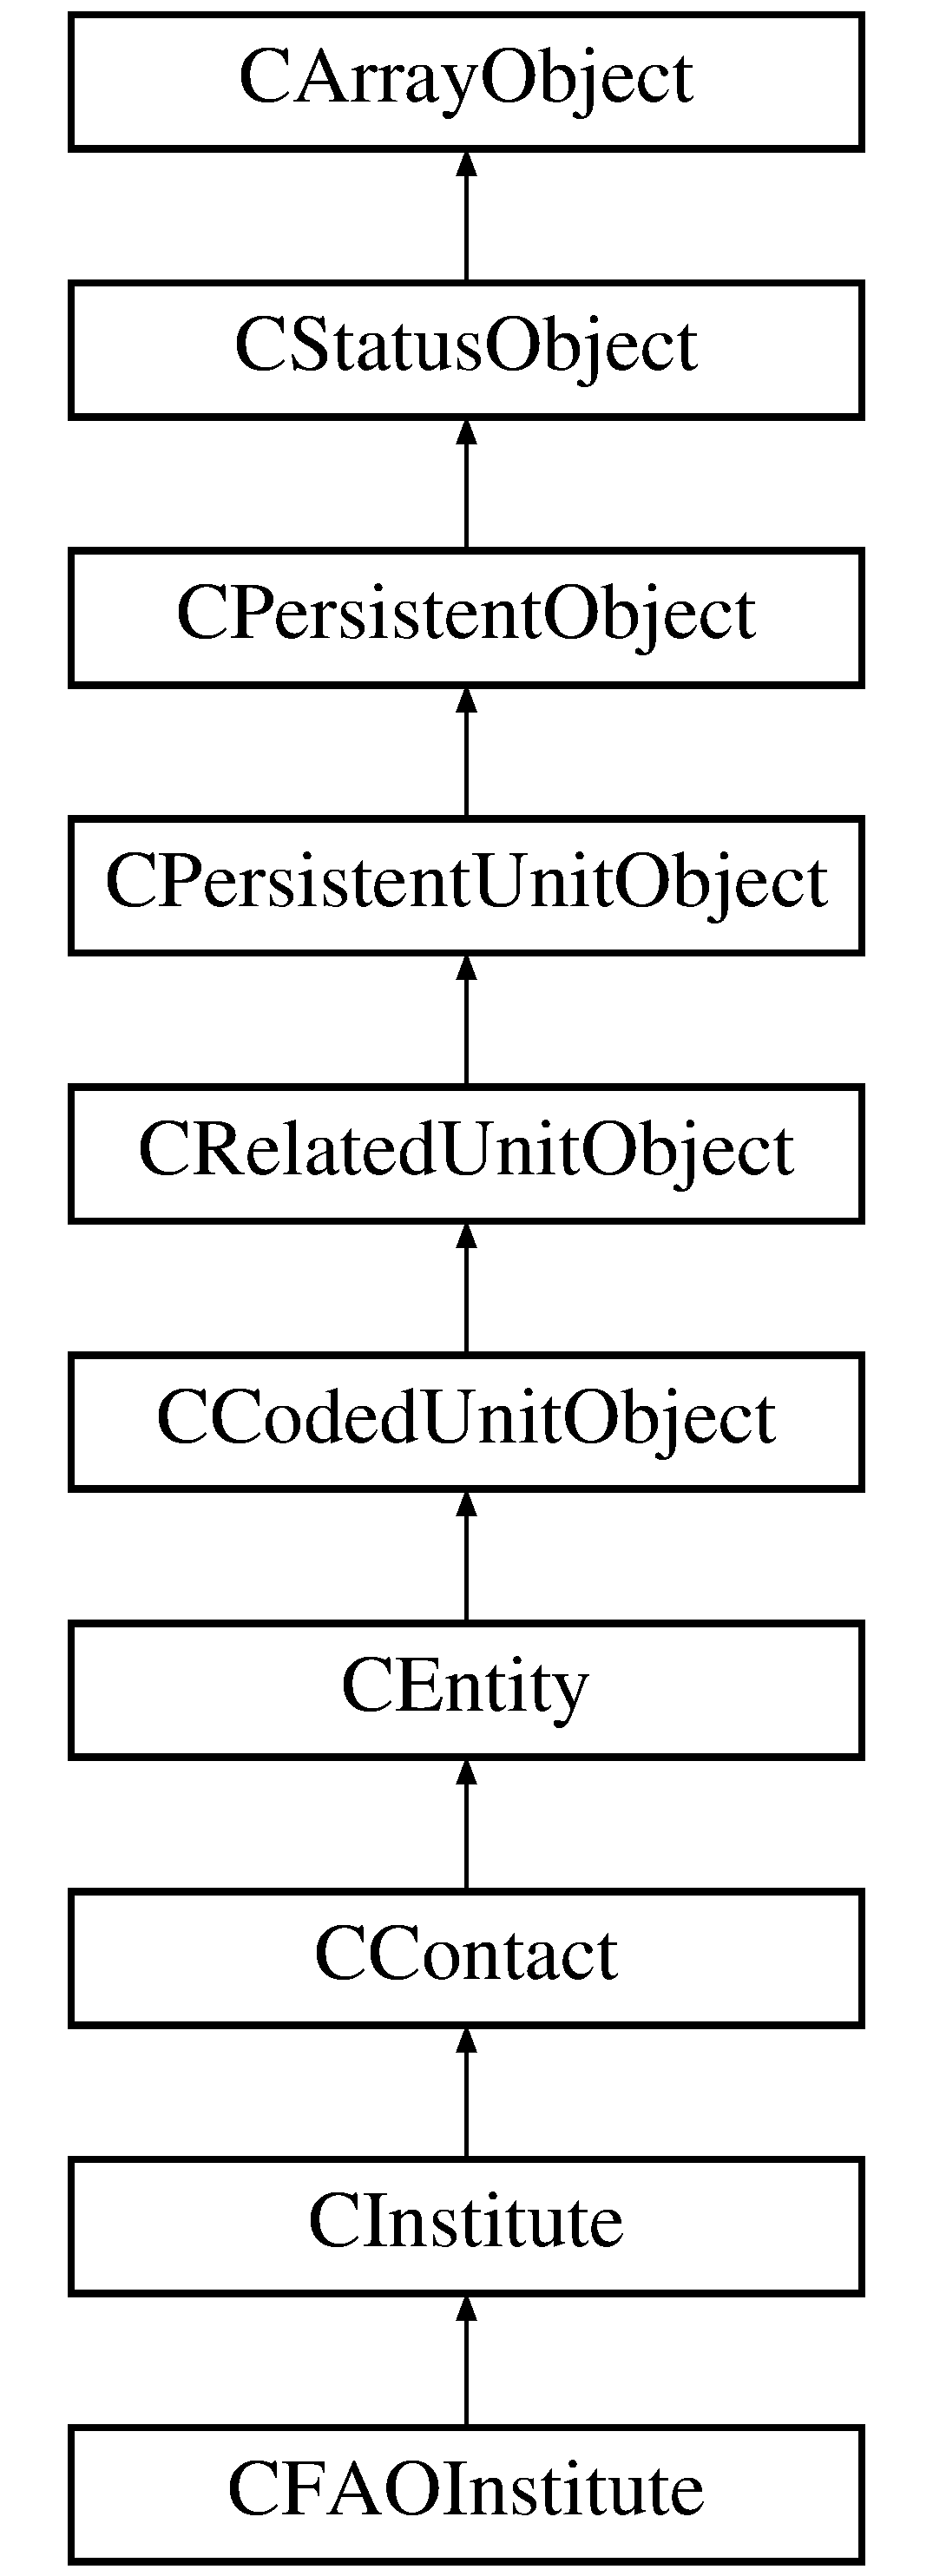
\includegraphics[height=10.000000cm]{class_c_contact}
\end{center}
\end{figure}
\subsection*{Public Member Functions}
\begin{DoxyCompactItemize}
\item 
\hyperlink{class_c_contact_aea135ec858be3986169b3764863455fd}{Mail} (\$the\-Value=N\-U\-L\-L, \$the\-Type=N\-U\-L\-L, \$get\-Old=F\-A\-L\-S\-E)
\item 
\hyperlink{class_c_contact_a33e959eb4723a50a402b0e573ec667ae}{Phone} (\$the\-Value=N\-U\-L\-L, \$the\-Type=N\-U\-L\-L, \$get\-Old=F\-A\-L\-S\-E)
\item 
\hyperlink{class_c_contact_aa2e82c640fc517c515ed9714de2e58e2}{Fax} (\$the\-Value=N\-U\-L\-L, \$the\-Type=N\-U\-L\-L, \$get\-Old=F\-A\-L\-S\-E)
\end{DoxyCompactItemize}
\subsection*{Additional Inherited Members}


\subsection{Member Function Documentation}
\hypertarget{class_c_contact_aa2e82c640fc517c515ed9714de2e58e2}{\index{C\-Contact@{C\-Contact}!Fax@{Fax}}
\index{Fax@{Fax}!CContact@{C\-Contact}}
\subsubsection[{Fax}]{\setlength{\rightskip}{0pt plus 5cm}C\-Contact\-::\-Fax (
\begin{DoxyParamCaption}
\item[{}]{\$the\-Value = {\ttfamily NULL}, }
\item[{}]{\$the\-Type = {\ttfamily NULL}, }
\item[{}]{\$get\-Old = {\ttfamily FALSE}}
\end{DoxyParamCaption}
)}}\label{class_c_contact_aa2e82c640fc517c515ed9714de2e58e2}
Manage telefax numbers.

This method can be used to manage the contact \hyperlink{}{telephone} numbers, it manages an array of strings with the following offsets\-:


\begin{DoxyItemize}
\item {\itshape \hyperlink{}{k\-T\-A\-G\-\_\-\-K\-I\-N\-D}}\-: The telephone number kind, this could be {\itshape home}, {\itshape work} or {\itshape other}. This element represents the array key, although technically it is implemented as an element to allow searching on all values. 
\item {\itshape \hyperlink{}{k\-T\-A\-G\-\_\-\-D\-A\-T\-A}}\-: The telephone number string, this element should hold the actual phone number. 
\end{DoxyItemize}

The parameters to this method are\-:


\begin{DoxyItemize}
\item {\bfseries \$the\-Value}\-: The value or operation\-: 
\begin{DoxyItemize}
\item {\itshape N\-U\-L\-L}\-: Return the current value selected by the second parameter. 
\item {\itshape F\-A\-L\-S\-E}\-: Delete the value selected by the second parameter. 
\item {\itshape other}\-: Set value selected by the second parameter. 
\end{DoxyItemize}
\item {\bfseries \$the\-Type}\-: The element type, kind or index\-: 
\begin{DoxyItemize}
\item {\itshape N\-U\-L\-L}\-: This value indicates that the phone has no type or kind, in general, when adding elements, this case applies to default elements. 
\item {\itshape other}\-: All other types will be interpreted as the kind or type of the phone number. 
\end{DoxyItemize}
\item {\bfseries \$get\-Old}\-: Determines what the method will return\-: 
\begin{DoxyItemize}
\item {\itshape T\-R\-U\-E}\-: Return the value {\itshape before} it was eventually modified. 
\item {\itshape F\-A\-L\-S\-E}\-: Return the value {\itshape after} it was eventually modified. 
\end{DoxyItemize}
\end{DoxyItemize}


\begin{DoxyParams}[1]{Parameters}
string & {\em \$the\-Value} & Telephone number or operation. \\
\hline
mixed & {\em \$the\-Type} & Mailing address kind or index. \\
\hline
boolean & {\em \$get\-Old} & T\-R\-U\-E get old value.\\
\hline
\end{DoxyParams}
public \begin{DoxyReturn}{Returns}
string 
\end{DoxyReturn}
\hypertarget{class_c_contact_aea135ec858be3986169b3764863455fd}{\index{C\-Contact@{C\-Contact}!Mail@{Mail}}
\index{Mail@{Mail}!CContact@{C\-Contact}}
\subsubsection[{Mail}]{\setlength{\rightskip}{0pt plus 5cm}C\-Contact\-::\-Mail (
\begin{DoxyParamCaption}
\item[{}]{\$the\-Value = {\ttfamily NULL}, }
\item[{}]{\$the\-Type = {\ttfamily NULL}, }
\item[{}]{\$get\-Old = {\ttfamily FALSE}}
\end{DoxyParamCaption}
)}}\label{class_c_contact_aea135ec858be3986169b3764863455fd}
Manage mailing address.

This method can be used to manage the contact \hyperlink{}{mailing} address, it manages an array of structures with the following offsets\-:


\begin{DoxyItemize}
\item {\itshape \hyperlink{}{k\-T\-A\-G\-\_\-\-K\-I\-N\-D}}\-: The mailing address kind, this could be {\itshape home}, {\itshape work} or {\itshape other}. This element represents the array key, although technically it is implemented as an element to allow searching on all values. 
\item {\itshape \hyperlink{}{k\-T\-A\-G\-\_\-\-D\-A\-T\-A}}\-: The mailing address structure or string, this element should hold the actual address. 
\end{DoxyItemize}

The parameters to this method are\-:


\begin{DoxyItemize}
\item {\bfseries \$the\-Value}\-: The value or operation\-: 
\begin{DoxyItemize}
\item {\itshape N\-U\-L\-L}\-: Return the current value selected by the second parameter. 
\item {\itshape F\-A\-L\-S\-E}\-: Delete the value selected by the second parameter. 
\item {\itshape other}\-: Set value selected by the second parameter. 
\end{DoxyItemize}
\item {\bfseries \$the\-Type}\-: The element type, kind or index\-: 
\begin{DoxyItemize}
\item {\itshape N\-U\-L\-L}\-: This value indicates that the adress has no type or kind, in general, when adding elements, this case applies to default elements. 
\item {\itshape other}\-: All other types will be interpreted as the kind or type of the address. 
\end{DoxyItemize}
\item {\bfseries \$get\-Old}\-: Determines what the method will return\-: 
\begin{DoxyItemize}
\item {\itshape T\-R\-U\-E}\-: Return the value {\itshape before} it was eventually modified. 
\item {\itshape F\-A\-L\-S\-E}\-: Return the value {\itshape after} it was eventually modified. 
\end{DoxyItemize}
\end{DoxyItemize}


\begin{DoxyParams}[1]{Parameters}
mixed & {\em \$the\-Value} & Mailing address or operation. \\
\hline
mixed & {\em \$the\-Type} & Mailing address kind or index. \\
\hline
boolean & {\em \$get\-Old} & T\-R\-U\-E get old value.\\
\hline
\end{DoxyParams}
public \begin{DoxyReturn}{Returns}
string 
\end{DoxyReturn}
\hypertarget{class_c_contact_a33e959eb4723a50a402b0e573ec667ae}{\index{C\-Contact@{C\-Contact}!Phone@{Phone}}
\index{Phone@{Phone}!CContact@{C\-Contact}}
\subsubsection[{Phone}]{\setlength{\rightskip}{0pt plus 5cm}C\-Contact\-::\-Phone (
\begin{DoxyParamCaption}
\item[{}]{\$the\-Value = {\ttfamily NULL}, }
\item[{}]{\$the\-Type = {\ttfamily NULL}, }
\item[{}]{\$get\-Old = {\ttfamily FALSE}}
\end{DoxyParamCaption}
)}}\label{class_c_contact_a33e959eb4723a50a402b0e573ec667ae}
Manage telephone numbers.

This method can be used to manage the contact \hyperlink{}{telephone} numbers, it manages an array of strings with the following offsets\-:


\begin{DoxyItemize}
\item {\itshape \hyperlink{}{k\-T\-A\-G\-\_\-\-K\-I\-N\-D}}\-: The telephone number kind, this could be {\itshape home}, {\itshape work} or {\itshape other}. This element represents the array key, although technically it is implemented as an element to allow searching on all values. 
\item {\itshape \hyperlink{}{k\-T\-A\-G\-\_\-\-D\-A\-T\-A}}\-: The telephone number string, this element should hold the actual phone number. 
\end{DoxyItemize}

The parameters to this method are\-:


\begin{DoxyItemize}
\item {\bfseries \$the\-Value}\-: The value or operation\-: 
\begin{DoxyItemize}
\item {\itshape N\-U\-L\-L}\-: Return the current value selected by the second parameter. 
\item {\itshape F\-A\-L\-S\-E}\-: Delete the value selected by the second parameter. 
\item {\itshape other}\-: Set value selected by the second parameter. 
\end{DoxyItemize}
\item {\bfseries \$the\-Type}\-: The element type, kind or index\-: 
\begin{DoxyItemize}
\item {\itshape N\-U\-L\-L}\-: This value indicates that the phone has no type or kind, in general, when adding elements, this case applies to default elements. 
\item {\itshape other}\-: All other types will be interpreted as the kind or type of the phone number. 
\end{DoxyItemize}
\item {\bfseries \$get\-Old}\-: Determines what the method will return\-: 
\begin{DoxyItemize}
\item {\itshape T\-R\-U\-E}\-: Return the value {\itshape before} it was eventually modified. 
\item {\itshape F\-A\-L\-S\-E}\-: Return the value {\itshape after} it was eventually modified. 
\end{DoxyItemize}
\end{DoxyItemize}


\begin{DoxyParams}[1]{Parameters}
string & {\em \$the\-Value} & Telephone number or operation. \\
\hline
mixed & {\em \$the\-Type} & Mailing address kind or index. \\
\hline
boolean & {\em \$get\-Old} & T\-R\-U\-E get old value.\\
\hline
\end{DoxyParams}
public \begin{DoxyReturn}{Returns}
string 
\end{DoxyReturn}


The documentation for this class was generated from the following file\-:\begin{DoxyCompactItemize}
\item 
/\-Library/\-Web\-Server/\-Library/wrapper/classes/C\-Contact.\-php\end{DoxyCompactItemize}

\hypertarget{class_c_container}{\section{C\-Container Class Reference}
\label{class_c_container}\index{C\-Container@{C\-Container}}
}
Inheritance diagram for C\-Container\-:\begin{figure}[H]
\begin{center}
\leavevmode
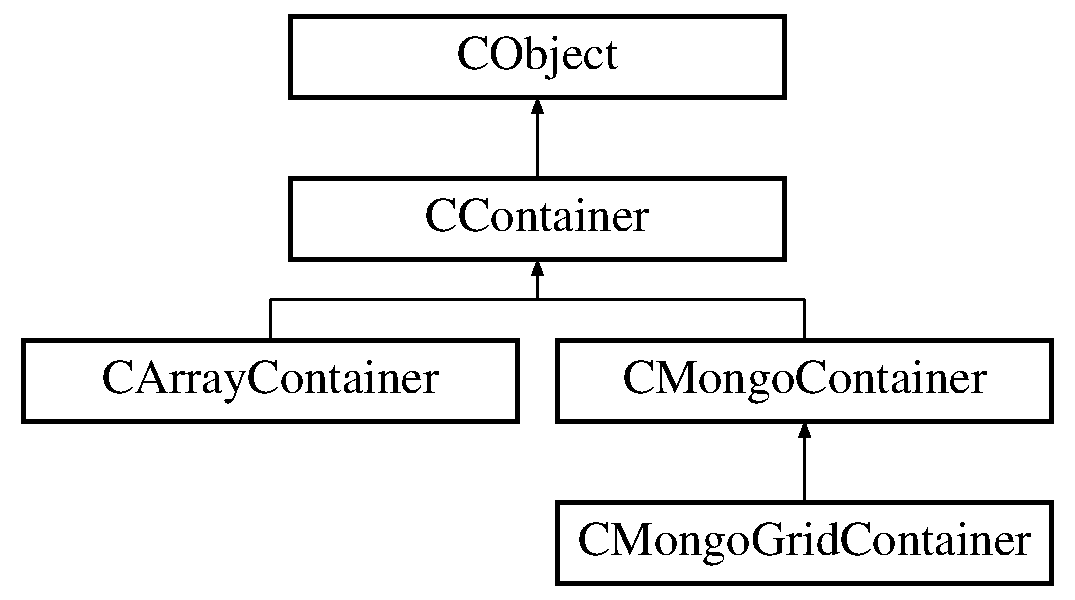
\includegraphics[height=4.000000cm]{class_c_container}
\end{center}
\end{figure}
\subsection*{Public Member Functions}
\begin{DoxyCompactItemize}
\item 
\hyperlink{class_c_container_af2fc42b4d7b5f71e0f127c941440b1aa}{\-\_\-\-\_\-construct} (\$the\-Container=N\-U\-L\-L)
\item 
\hyperlink{class_c_container_aa1d6ed5052f55cdffcf6445968f203ed}{\-\_\-\-\_\-to\-String} ()
\item 
\hyperlink{class_c_container_a7d10fa70dfa381cb95e66c265e2ca113}{Container} (\$the\-Value=N\-U\-L\-L, \$get\-Old=F\-A\-L\-S\-E)
\item 
\hyperlink{class_c_container_a0d691b62d9b70b924e24a332931ce9d1}{Database} ()
\item 
\hyperlink{class_c_container_a4847dc676d1f7704e75f8981e927508a}{Commit} (\&\$the\-Object, \$the\-Identifier=N\-U\-L\-L, \$the\-Modifiers=k\-F\-L\-A\-G\-\_\-\-P\-E\-R\-S\-I\-S\-T\-\_\-\-R\-E\-P\-L\-A\-C\-E)
\item 
\hyperlink{class_c_container_a48db96aa6bbf15d0bfc15725616b7154}{Load} (\$the\-Identifier, \$the\-Modifiers=k\-F\-L\-A\-G\-\_\-\-D\-E\-F\-A\-U\-L\-T)
\item 
\hyperlink{class_c_container_aa91ec2f4624a2ebfb74668f274139329}{Delete} (\$the\-Identifier, \$the\-Modifiers=k\-F\-L\-A\-G\-\_\-\-D\-E\-F\-A\-U\-L\-T)
\item 
\hyperlink{class_c_container_a1486a3cb34d24ff1c3028ad4360b5dc6}{Reference} (\$the\-Object, \$the\-Modifiers=k\-F\-L\-A\-G\-\_\-\-R\-E\-F\-E\-R\-E\-N\-C\-E\-\_\-\-I\-D\-E\-N\-T\-I\-F\-I\-E\-R)
\item 
\hyperlink{class_c_container_aa339d3c4c9b011713176a89fe9c7783d}{Unserialise\-Object} (\&\$the\-Object)
\item 
\hyperlink{class_c_container_a09d585e2a9809221a42d52d7520c9cbf}{Unserialise\-Data} (\&\$the\-Element)
\end{DoxyCompactItemize}
\subsection*{Protected Member Functions}
\begin{DoxyCompactItemize}
\item 
\& \hyperlink{class_c_container_a4794d326f4ffd3c2b8afd2e0460604ff}{\-\_\-\-Container} ()
\item 
\hyperlink{class_c_container_acbc85dd164615b31c9edfec93bcf27f9}{\-\_\-\-Commit} (\&\$the\-Object, \&\$the\-Identifier, \&\$the\-Modifiers)
\item 
\hyperlink{class_c_container_a865f140560991fa21a88b7fc8ff8f1f5}{\-\_\-\-Load} (\&\$the\-Identifier, \&\$the\-Modifiers)
\item 
\hyperlink{class_c_container_a20aac3eec154c2122f2c602bf5ce35fe}{\-\_\-\-Delete} (\&\$the\-Identifier, \&\$the\-Modifiers)
\item 
\hyperlink{class_c_container_a0dc47e54abc533cedf1c2c0f915d96b2}{\-\_\-\-Prepare\-Commit} (\&\$the\-Object, \&\$the\-Identifier, \&\$the\-Modifiers)
\item 
\hyperlink{class_c_container_a1b84868c32fcfd3e11a9f6cc85fc461c}{\-\_\-\-Prepare\-Load} (\&\$the\-Identifier, \&\$the\-Modifiers)
\item 
\hyperlink{class_c_container_a238776ec6152dd400be2ed87ba949fd0}{\-\_\-\-Prepare\-Delete} (\&\$the\-Identifier, \&\$the\-Modifiers)
\item 
\hyperlink{class_c_container_a4c9cae709a81dd53c7307bfbde891fae}{\-\_\-\-Finish\-Commit} (\&\$the\-Object, \&\$the\-Identifier, \&\$the\-Modifiers)
\item 
\hyperlink{class_c_container_ab53bd683f0e28b2203897cf03f9d1c76}{\-\_\-\-Finish\-Load} (\&\$the\-Object, \&\$the\-Identifier, \&\$the\-Modifiers)
\item 
\hyperlink{class_c_container_ab8bfc9866573dd474dcf418059d94fbe}{\-\_\-\-Finish\-Delete} (\&\$the\-Object, \&\$the\-Identifier, \&\$the\-Modifiers)
\end{DoxyCompactItemize}
\subsection*{Protected Attributes}
\begin{DoxyCompactItemize}
\item 
\hypertarget{class_c_container_a52a8e4284fff9530c1ff25c93b238b9f}{{\bfseries \$m\-Container} = N\-U\-L\-L}\label{class_c_container_a52a8e4284fff9530c1ff25c93b238b9f}

\end{DoxyCompactItemize}
\subsection*{Additional Inherited Members}


\subsection{Constructor \& Destructor Documentation}
\hypertarget{class_c_container_af2fc42b4d7b5f71e0f127c941440b1aa}{\index{C\-Container@{C\-Container}!\-\_\-\-\_\-construct@{\-\_\-\-\_\-construct}}
\index{\-\_\-\-\_\-construct@{\-\_\-\-\_\-construct}!CContainer@{C\-Container}}
\subsubsection[{\-\_\-\-\_\-construct}]{\setlength{\rightskip}{0pt plus 5cm}C\-Container\-::\-\_\-\-\_\-construct (
\begin{DoxyParamCaption}
\item[{}]{\$the\-Container = {\ttfamily NULL}}
\end{DoxyParamCaption}
)}}\label{class_c_container_af2fc42b4d7b5f71e0f127c941440b1aa}
Instantiate class.

You instantiate the class with a native data store, the method expects a single parameter that will be handled specifically by specialised derived classes.

Derived classes should overload this method if a default value is possible; to check for specific container types they should rather overload the member accessor \hyperlink{class_c_container_a7d10fa70dfa381cb95e66c265e2ca113}{method}.


\begin{DoxyParams}[1]{Parameters}
mixed & {\em \$the\-Container} & Native object store.\\
\hline
\end{DoxyParams}
public

\hyperlink{class_c_container_a7d10fa70dfa381cb95e66c265e2ca113}{Container()} 

Reimplemented in \hyperlink{class_c_array_container_a10e83176c2a2ee0d9fe53ca9e51b0ca0}{C\-Array\-Container}.



\subsection{Member Function Documentation}
\hypertarget{class_c_container_aa1d6ed5052f55cdffcf6445968f203ed}{\index{C\-Container@{C\-Container}!\-\_\-\-\_\-to\-String@{\-\_\-\-\_\-to\-String}}
\index{\-\_\-\-\_\-to\-String@{\-\_\-\-\_\-to\-String}!CContainer@{C\-Container}}
\subsubsection[{\-\_\-\-\_\-to\-String}]{\setlength{\rightskip}{0pt plus 5cm}C\-Container\-::\-\_\-\-\_\-to\-String (
\begin{DoxyParamCaption}
{}
\end{DoxyParamCaption}
)\hspace{0.3cm}{\ttfamily [abstract]}}}\label{class_c_container_aa1d6ed5052f55cdffcf6445968f203ed}
Return container name.

This method should return the current container's name.

All derived concrete classes should implement this method, all containers must be able to return a name.

public \begin{DoxyReturn}{Returns}
string 
\end{DoxyReturn}


Reimplemented in \hyperlink{class_c_array_container_aa7739e1def0a13a6750d6fa722952bcc}{C\-Array\-Container}, and \hyperlink{class_c_mongo_container_abc325eae251667da577efdb45a7d3c17}{C\-Mongo\-Container}.

\hypertarget{class_c_container_acbc85dd164615b31c9edfec93bcf27f9}{\index{C\-Container@{C\-Container}!\-\_\-\-Commit@{\-\_\-\-Commit}}
\index{\-\_\-\-Commit@{\-\_\-\-Commit}!CContainer@{C\-Container}}
\subsubsection[{\-\_\-\-Commit}]{\setlength{\rightskip}{0pt plus 5cm}C\-Container\-::\-\_\-\-Commit (
\begin{DoxyParamCaption}
\item[{\&}]{\$the\-Object, }
\item[{\&}]{\$the\-Identifier, }
\item[{\&}]{\$the\-Modifiers}
\end{DoxyParamCaption}
)\hspace{0.3cm}{\ttfamily [abstract]}, {\ttfamily [protected]}}}\label{class_c_container_acbc85dd164615b31c9edfec93bcf27f9}
Commit provided object.

Derived classes must implement this method to actually store the provided object in the container, the method expects the same parameters as the public \hyperlink{class_c_container_a4847dc676d1f7704e75f8981e927508a}{interface}, except that in this method these are passed by reference.

The method should return the object's key within the container or raise an exception if the operation was not successful.


\begin{DoxyParams}[1]{Parameters}
reference & {\em \&\$the\-Object} & Object to commit. \\
\hline
reference & {\em \&\$the\-Identifier} & Object identifier. \\
\hline
reference & {\em \&\$the\-Modifiers} & Commit modifiers.\\
\hline
\end{DoxyParams}
protected \begin{DoxyReturn}{Returns}
mixed 
\end{DoxyReturn}


Reimplemented in \hyperlink{class_c_mongo_container_a92cbcdba4f2b0bda2ae3eeb7a08d7ba2}{C\-Mongo\-Container}, \hyperlink{class_c_array_container_a8f58eaea0751d43e4ac7a5d4c732ddaa}{C\-Array\-Container}, and \hyperlink{class_c_mongo_grid_container_a1dc8378e77df7c06afc2c733e2422482}{C\-Mongo\-Grid\-Container}.

\hypertarget{class_c_container_a4794d326f4ffd3c2b8afd2e0460604ff}{\index{C\-Container@{C\-Container}!\-\_\-\-Container@{\-\_\-\-Container}}
\index{\-\_\-\-Container@{\-\_\-\-Container}!CContainer@{C\-Container}}
\subsubsection[{\-\_\-\-Container}]{\setlength{\rightskip}{0pt plus 5cm}\& C\-Container\-::\-\_\-\-Container (
\begin{DoxyParamCaption}
{}
\end{DoxyParamCaption}
)\hspace{0.3cm}{\ttfamily [protected]}}}\label{class_c_container_a4794d326f4ffd3c2b8afd2e0460604ff}
Get container reference.

This method can be used to retrieve a reference to the native container member, this can be useful when the native \hyperlink{class_c_container_a7d10fa70dfa381cb95e66c265e2ca113}{container} is not an object passed by reference.

protected \begin{DoxyReturn}{Returns}
mixed 
\end{DoxyReturn}
\hypertarget{class_c_container_a20aac3eec154c2122f2c602bf5ce35fe}{\index{C\-Container@{C\-Container}!\-\_\-\-Delete@{\-\_\-\-Delete}}
\index{\-\_\-\-Delete@{\-\_\-\-Delete}!CContainer@{C\-Container}}
\subsubsection[{\-\_\-\-Delete}]{\setlength{\rightskip}{0pt plus 5cm}C\-Container\-::\-\_\-\-Delete (
\begin{DoxyParamCaption}
\item[{\&}]{\$the\-Identifier, }
\item[{\&}]{\$the\-Modifiers}
\end{DoxyParamCaption}
)\hspace{0.3cm}{\ttfamily [abstract]}, {\ttfamily [protected]}}}\label{class_c_container_a20aac3eec154c2122f2c602bf5ce35fe}
Load object.

Derived classes must implement this method to actually remove the object from the container, the method expects the same parameters as the public \hyperlink{class_c_container_aa91ec2f4624a2ebfb74668f274139329}{interface}, except that in this method these are passed by reference.

The method should return the removed object or {\itshape N\-U\-L\-L} if not found.


\begin{DoxyParams}[1]{Parameters}
reference & {\em \&\$the\-Identifier} & Object identifier. \\
\hline
reference & {\em \&\$the\-Modifiers} & Delete modifiers.\\
\hline
\end{DoxyParams}
protected \begin{DoxyReturn}{Returns}
mixed 
\end{DoxyReturn}


Reimplemented in \hyperlink{class_c_mongo_container_aa516a049efe0c9083e2f8c5b9f9076a4}{C\-Mongo\-Container}, and \hyperlink{class_c_array_container_ac8469e57be785cd45142fdaf0419bf8f}{C\-Array\-Container}.

\hypertarget{class_c_container_a4c9cae709a81dd53c7307bfbde891fae}{\index{C\-Container@{C\-Container}!\-\_\-\-Finish\-Commit@{\-\_\-\-Finish\-Commit}}
\index{\-\_\-\-Finish\-Commit@{\-\_\-\-Finish\-Commit}!CContainer@{C\-Container}}
\subsubsection[{\-\_\-\-Finish\-Commit}]{\setlength{\rightskip}{0pt plus 5cm}C\-Container\-::\-\_\-\-Finish\-Commit (
\begin{DoxyParamCaption}
\item[{\&}]{\$the\-Object, }
\item[{\&}]{\$the\-Identifier, }
\item[{\&}]{\$the\-Modifiers}
\end{DoxyParamCaption}
)\hspace{0.3cm}{\ttfamily [protected]}}}\label{class_c_container_a4c9cae709a81dd53c7307bfbde891fae}
Normalise after a \hyperlink{class_c_container_acbc85dd164615b31c9edfec93bcf27f9}{store}.

The duty of this method is to clean up or restore the object after the \hyperlink{class_c_container_acbc85dd164615b31c9edfec93bcf27f9}{store} operation.

By default we perform the following checks\-:


\begin{DoxyItemize}
\item \hyperlink{class_c_data_type_a608d6fc184bce537ce83669f729d6008}{Serialise} the object if \hyperlink{}{necessary}. 
\item \hyperlink{class_c_data_type_a1cae522eec386d293b6087a99e9a8b0b}{Serialise} the identifier if \hyperlink{}{necessary}. 
\end{DoxyItemize}

In derived classes you should always call the parent method, remember to check this method to determine whether to implement your custom changes before or after calling this method.


\begin{DoxyParams}[1]{Parameters}
reference & {\em \&\$the\-Object} & Object or data. \\
\hline
reference & {\em \&\$the\-Identifier} & Object identifier. \\
\hline
reference & {\em \&\$the\-Modifiers} & Commit modifiers.\\
\hline
\end{DoxyParams}
protected

\hyperlink{class_c_data_type_a608d6fc184bce537ce83669f729d6008}{C\-Data\-Type\-::\-Serialise\-Object()}  \hyperlink{class_c_data_type_a1cae522eec386d293b6087a99e9a8b0b}{C\-Data\-Type\-::\-Serialise\-Data()}

\begin{DoxySeeAlso}{See Also}
k\-F\-L\-A\-G\-\_\-\-S\-T\-A\-T\-E\-\_\-\-E\-N\-C\-O\-D\-E\-D 
\end{DoxySeeAlso}
\hypertarget{class_c_container_ab8bfc9866573dd474dcf418059d94fbe}{\index{C\-Container@{C\-Container}!\-\_\-\-Finish\-Delete@{\-\_\-\-Finish\-Delete}}
\index{\-\_\-\-Finish\-Delete@{\-\_\-\-Finish\-Delete}!CContainer@{C\-Container}}
\subsubsection[{\-\_\-\-Finish\-Delete}]{\setlength{\rightskip}{0pt plus 5cm}C\-Container\-::\-\_\-\-Finish\-Delete (
\begin{DoxyParamCaption}
\item[{\&}]{\$the\-Object, }
\item[{\&}]{\$the\-Identifier, }
\item[{\&}]{\$the\-Modifiers}
\end{DoxyParamCaption}
)\hspace{0.3cm}{\ttfamily [protected]}}}\label{class_c_container_ab8bfc9866573dd474dcf418059d94fbe}
Normalise after a store.

The duty of this method is to clean up or restore the object after the \hyperlink{class_c_container_a20aac3eec154c2122f2c602bf5ce35fe}{delete} operation.

By default we perform the following checks\-:


\begin{DoxyItemize}
\item \hyperlink{class_c_data_type_a1cae522eec386d293b6087a99e9a8b0b}{Serialise} the identifier if \hyperlink{}{necessary}. 
\end{DoxyItemize}

In derived classes you should always call the parent method, remember to check this method to determine whether to implement your custom changes before or after calling this method.


\begin{DoxyParams}[1]{Parameters}
reference & {\em \&\$the\-Object} & Object or data. \\
\hline
reference & {\em \&\$the\-Identifier} & Object identifier. \\
\hline
reference & {\em \&\$the\-Modifiers} & Commit modifiers.\\
\hline
\end{DoxyParams}
protected

\hyperlink{class_c_data_type_a1cae522eec386d293b6087a99e9a8b0b}{C\-Data\-Type\-::\-Serialise\-Data()}

\begin{DoxySeeAlso}{See Also}
k\-F\-L\-A\-G\-\_\-\-S\-T\-A\-T\-E\-\_\-\-E\-N\-C\-O\-D\-E\-D 
\end{DoxySeeAlso}
\hypertarget{class_c_container_ab53bd683f0e28b2203897cf03f9d1c76}{\index{C\-Container@{C\-Container}!\-\_\-\-Finish\-Load@{\-\_\-\-Finish\-Load}}
\index{\-\_\-\-Finish\-Load@{\-\_\-\-Finish\-Load}!CContainer@{C\-Container}}
\subsubsection[{\-\_\-\-Finish\-Load}]{\setlength{\rightskip}{0pt plus 5cm}C\-Container\-::\-\_\-\-Finish\-Load (
\begin{DoxyParamCaption}
\item[{\&}]{\$the\-Object, }
\item[{\&}]{\$the\-Identifier, }
\item[{\&}]{\$the\-Modifiers}
\end{DoxyParamCaption}
)\hspace{0.3cm}{\ttfamily [protected]}}}\label{class_c_container_ab53bd683f0e28b2203897cf03f9d1c76}
Normalise after a \hyperlink{class_c_container_a865f140560991fa21a88b7fc8ff8f1f5}{load}.

The duty of this method is to clean up or restore the object after the \hyperlink{class_c_container_a865f140560991fa21a88b7fc8ff8f1f5}{load} operation.

By default we perform the following checks\-:


\begin{DoxyItemize}
\item \hyperlink{class_c_data_type_a608d6fc184bce537ce83669f729d6008}{Serialise} the object if \hyperlink{}{necessary}. 
\item \hyperlink{class_c_data_type_a1cae522eec386d293b6087a99e9a8b0b}{Serialise} the identifier if \hyperlink{}{necessary}. 
\end{DoxyItemize}

In derived classes you should always call the parent method, remember to check this method to determine whether to implement your custom changes before or after calling this method.


\begin{DoxyParams}[1]{Parameters}
reference & {\em \&\$the\-Object} & Object reference. \\
\hline
reference & {\em \&\$the\-Identifier} & Object identifier. \\
\hline
reference & {\em \&\$the\-Modifiers} & Commit modifiers.\\
\hline
\end{DoxyParams}
protected

\hyperlink{class_c_data_type_a608d6fc184bce537ce83669f729d6008}{C\-Data\-Type\-::\-Serialise\-Object()}  \hyperlink{class_c_data_type_a1cae522eec386d293b6087a99e9a8b0b}{C\-Data\-Type\-::\-Serialise\-Data()}

\begin{DoxySeeAlso}{See Also}
k\-F\-L\-A\-G\-\_\-\-S\-T\-A\-T\-E\-\_\-\-E\-N\-C\-O\-D\-E\-D 
\end{DoxySeeAlso}
\hypertarget{class_c_container_a865f140560991fa21a88b7fc8ff8f1f5}{\index{C\-Container@{C\-Container}!\-\_\-\-Load@{\-\_\-\-Load}}
\index{\-\_\-\-Load@{\-\_\-\-Load}!CContainer@{C\-Container}}
\subsubsection[{\-\_\-\-Load}]{\setlength{\rightskip}{0pt plus 5cm}C\-Container\-::\-\_\-\-Load (
\begin{DoxyParamCaption}
\item[{\&}]{\$the\-Identifier, }
\item[{\&}]{\$the\-Modifiers}
\end{DoxyParamCaption}
)\hspace{0.3cm}{\ttfamily [abstract]}, {\ttfamily [protected]}}}\label{class_c_container_a865f140560991fa21a88b7fc8ff8f1f5}
Load object.

Derived classes must implement this method to actually retrieve the provided object from the container, the method expects the same parameters as the public \hyperlink{class_c_container_a48db96aa6bbf15d0bfc15725616b7154}{interface}, except that in this method these are passed by reference.

The method should return the found object or {\itshape N\-U\-L\-L} if not found.


\begin{DoxyParams}[1]{Parameters}
reference & {\em \&\$the\-Identifier} & Object identifier. \\
\hline
reference & {\em \&\$the\-Modifiers} & Load modifiers.\\
\hline
\end{DoxyParams}
protected \begin{DoxyReturn}{Returns}
mixed 
\end{DoxyReturn}


Reimplemented in \hyperlink{class_c_mongo_container_a61f469d1975834b22665392542620317}{C\-Mongo\-Container}.

\hypertarget{class_c_container_a0dc47e54abc533cedf1c2c0f915d96b2}{\index{C\-Container@{C\-Container}!\-\_\-\-Prepare\-Commit@{\-\_\-\-Prepare\-Commit}}
\index{\-\_\-\-Prepare\-Commit@{\-\_\-\-Prepare\-Commit}!CContainer@{C\-Container}}
\subsubsection[{\-\_\-\-Prepare\-Commit}]{\setlength{\rightskip}{0pt plus 5cm}C\-Container\-::\-\_\-\-Prepare\-Commit (
\begin{DoxyParamCaption}
\item[{\&}]{\$the\-Object, }
\item[{\&}]{\$the\-Identifier, }
\item[{\&}]{\$the\-Modifiers}
\end{DoxyParamCaption}
)\hspace{0.3cm}{\ttfamily [protected]}}}\label{class_c_container_a0dc47e54abc533cedf1c2c0f915d96b2}
Prepare before a \hyperlink{class_c_container_acbc85dd164615b31c9edfec93bcf27f9}{commit}.

This method will be called before the \hyperlink{class_c_container_acbc85dd164615b31c9edfec93bcf27f9}{store} operation, its duty is to prepare the object and check the parameters, please refer to \hyperlink{class_c_container_a4847dc676d1f7704e75f8981e927508a}{this} documentation for a reference of the method's parameters. Note that in this method all three parameters are passed by reference.

By default we perform the following checks\-:


\begin{DoxyItemize}
\item Ensure the current object has a container. 
\item Ensure the identifier is provided if the operation is not an \hyperlink{}{insert}. 
\item Ensure the method has the correct options. 
\item Get the \hyperlink{class_c_persistent_object_aa8dc7db66e2af3d28c2035161a2aabf9}{encoded} status \hyperlink{}{flag} from the object and pass it to the current container. 
\item \hyperlink{class_c_container_aa339d3c4c9b011713176a89fe9c7783d}{Unserialise} the object if \hyperlink{}{necessary}. 
\item \hyperlink{class_c_container_a09d585e2a9809221a42d52d7520c9cbf}{Unserialise} the identifier if \hyperlink{}{necessary}. 
\end{DoxyItemize}

In derived classes you should always call the parent method, remember to check this method to determine whether to implement your custom changes before or after calling this method.


\begin{DoxyParams}[1]{Parameters}
reference & {\em \&\$the\-Object} & Object or data. \\
\hline
reference & {\em \&\$the\-Identifier} & Object identifier. \\
\hline
reference & {\em \&\$the\-Modifiers} & Commit modifiers.\\
\hline
\end{DoxyParams}
protected


\begin{DoxyExceptions}{Exceptions}
{\em \{@link} & \hyperlink{class_c_exception}{C\-Exception} \hyperlink{class_c_exception}{C\-Exception}\}\\
\hline
\end{DoxyExceptions}
\hyperlink{class_c_container_a7d10fa70dfa381cb95e66c265e2ca113}{Container()}  \hyperlink{class_c_container_aa339d3c4c9b011713176a89fe9c7783d}{Unserialise\-Object()}  \hyperlink{class_c_container_a09d585e2a9809221a42d52d7520c9cbf}{Unserialise\-Data()}

\begin{DoxySeeAlso}{See Also}
k\-F\-L\-A\-G\-\_\-\-S\-T\-A\-T\-E\-\_\-\-E\-N\-C\-O\-D\-E\-D 
\end{DoxySeeAlso}


Reimplemented in \hyperlink{class_c_mongo_container_af592e4500a640190f374c18683af3b83}{C\-Mongo\-Container}, \hyperlink{class_c_array_container_ad77352799ccd0807013a133ccf5fd2bc}{C\-Array\-Container}, and \hyperlink{class_c_mongo_grid_container_a94715c26002c38020a8e4103d3075426}{C\-Mongo\-Grid\-Container}.

\hypertarget{class_c_container_a238776ec6152dd400be2ed87ba949fd0}{\index{C\-Container@{C\-Container}!\-\_\-\-Prepare\-Delete@{\-\_\-\-Prepare\-Delete}}
\index{\-\_\-\-Prepare\-Delete@{\-\_\-\-Prepare\-Delete}!CContainer@{C\-Container}}
\subsubsection[{\-\_\-\-Prepare\-Delete}]{\setlength{\rightskip}{0pt plus 5cm}C\-Container\-::\-\_\-\-Prepare\-Delete (
\begin{DoxyParamCaption}
\item[{\&}]{\$the\-Identifier, }
\item[{\&}]{\$the\-Modifiers}
\end{DoxyParamCaption}
)\hspace{0.3cm}{\ttfamily [protected]}}}\label{class_c_container_a238776ec6152dd400be2ed87ba949fd0}
Prepare before a \hyperlink{class_c_container_a20aac3eec154c2122f2c602bf5ce35fe}{delete}.

The duty of this method is to ensure that the parameters provided to the \hyperlink{class_c_container_a20aac3eec154c2122f2c602bf5ce35fe}{delete} operation are valid.

By default we perform the following checks\-:


\begin{DoxyItemize}
\item Ensure the current object has a container. 
\item Ensure the identifier is provided. 
\item \hyperlink{class_c_data_type_a1cae522eec386d293b6087a99e9a8b0b}{Serialise} the identifier if \hyperlink{}{necessary}. 
\end{DoxyItemize}

In derived classes you should always call the parent method, remember to check this method to determine whether to implement your custom changes before or after calling this method.


\begin{DoxyParams}[1]{Parameters}
reference & {\em \&\$the\-Identifier} & Object identifier. \\
\hline
reference & {\em \&\$the\-Modifiers} & Commit modifiers.\\
\hline
\end{DoxyParams}
protected


\begin{DoxyExceptions}{Exceptions}
{\em \{@link} & \hyperlink{class_c_exception}{C\-Exception} \hyperlink{class_c_exception}{C\-Exception}\}\\
\hline
\end{DoxyExceptions}
\hyperlink{class_c_container_a7d10fa70dfa381cb95e66c265e2ca113}{Container()}  \hyperlink{class_c_container_a09d585e2a9809221a42d52d7520c9cbf}{Unserialise\-Data()}

\begin{DoxySeeAlso}{See Also}
k\-F\-L\-A\-G\-\_\-\-S\-T\-A\-T\-E\-\_\-\-E\-N\-C\-O\-D\-E\-D 
\end{DoxySeeAlso}
\hypertarget{class_c_container_a1b84868c32fcfd3e11a9f6cc85fc461c}{\index{C\-Container@{C\-Container}!\-\_\-\-Prepare\-Load@{\-\_\-\-Prepare\-Load}}
\index{\-\_\-\-Prepare\-Load@{\-\_\-\-Prepare\-Load}!CContainer@{C\-Container}}
\subsubsection[{\-\_\-\-Prepare\-Load}]{\setlength{\rightskip}{0pt plus 5cm}C\-Container\-::\-\_\-\-Prepare\-Load (
\begin{DoxyParamCaption}
\item[{\&}]{\$the\-Identifier, }
\item[{\&}]{\$the\-Modifiers}
\end{DoxyParamCaption}
)\hspace{0.3cm}{\ttfamily [protected]}}}\label{class_c_container_a1b84868c32fcfd3e11a9f6cc85fc461c}
Prepare before a \hyperlink{class_c_container_a865f140560991fa21a88b7fc8ff8f1f5}{load}.

The duty of this method is to ensure that the parameters provided to the \hyperlink{class_c_container_a865f140560991fa21a88b7fc8ff8f1f5}{find} operation are valid.

By default we perform the following checks\-:


\begin{DoxyItemize}
\item Ensure the current object has a container. 
\item Ensure the identifier is provided. 
\item \hyperlink{class_c_data_type_a1cae522eec386d293b6087a99e9a8b0b}{Serialise} the identifier if \hyperlink{}{necessary}. 
\end{DoxyItemize}

In derived classes you should always call the parent method, remember to check this method to determine whether to implement your custom changes before or after calling this method.


\begin{DoxyParams}[1]{Parameters}
reference & {\em \&\$the\-Identifier} & Object identifier. \\
\hline
reference & {\em \&\$the\-Modifiers} & Create modifiers.\\
\hline
\end{DoxyParams}
protected


\begin{DoxyExceptions}{Exceptions}
{\em \{@link} & \hyperlink{class_c_exception}{C\-Exception} \hyperlink{class_c_exception}{C\-Exception}\}\\
\hline
\end{DoxyExceptions}
\hyperlink{class_c_container_a7d10fa70dfa381cb95e66c265e2ca113}{Container()}  \hyperlink{class_c_container_a09d585e2a9809221a42d52d7520c9cbf}{Unserialise\-Data()}

\begin{DoxySeeAlso}{See Also}
k\-F\-L\-A\-G\-\_\-\-S\-T\-A\-T\-E\-\_\-\-E\-N\-C\-O\-D\-E\-D 
\end{DoxySeeAlso}


Reimplemented in \hyperlink{class_c_mongo_container_a2c44e9229169abde420adf34045f5382}{C\-Mongo\-Container}.

\hypertarget{class_c_container_a4847dc676d1f7704e75f8981e927508a}{\index{C\-Container@{C\-Container}!Commit@{Commit}}
\index{Commit@{Commit}!CContainer@{C\-Container}}
\subsubsection[{Commit}]{\setlength{\rightskip}{0pt plus 5cm}C\-Container\-::\-Commit (
\begin{DoxyParamCaption}
\item[{\&}]{\$the\-Object, }
\item[{}]{\$the\-Identifier = {\ttfamily NULL}, }
\item[{}]{\$the\-Modifiers = {\ttfamily kFLAG\-\_\-PERSIST\-\_\-REPLACE}}
\end{DoxyParamCaption}
)}}\label{class_c_container_a4847dc676d1f7704e75f8981e927508a}
Commit provided object.

This method can be used to commit the provided object to the current data store, it expects three parameters\-:


\begin{DoxyItemize}
\item {\bfseries \$the\-Object}\-: The object or data to be committed. 
\item {\bfseries \$the\-Identifier}\-: This parameter is expected to be the object's unique identifier within the container, it will be the \hyperlink{class_c_container_a48db96aa6bbf15d0bfc15725616b7154}{access} key to the object once committed. If the value is {\itshape N\-U\-L\-L}, it means that it is the duty of the current container to set it, this will generally be the case when inserting objects; in all other cases the parameter is required. 
\item {\bfseries \$the\-Modifiers}\-: This parameter represents the commit operation options, by default we assume it is a bitfield where the following values apply\-: 
\begin{DoxyItemize}
\item {\itshape \hyperlink{}{k\-F\-L\-A\-G\-\_\-\-P\-E\-R\-S\-I\-S\-T\-\_\-\-I\-N\-S\-E\-R\-T}}\-: The provided object will be inserted in the container, it is assumed that no other element in the container shares the same identifier, in that case the method must raise an \hyperlink{}{exception}. 
\item {\itshape \hyperlink{}{k\-F\-L\-A\-G\-\_\-\-P\-E\-R\-S\-I\-S\-T\-\_\-\-U\-P\-D\-A\-T\-E}}\-: The provided object will replace the existing object. In this case the method expects the container to have an entry with the same key as the provided identifier, if this is not the case the method must raise an \hyperlink{}{exception}. With this option it is assumed that the provided object's attributes will replace all the existing object's ones. 
\item {\itshape \hyperlink{}{k\-F\-L\-A\-G\-\_\-\-P\-E\-R\-S\-I\-S\-T\-\_\-\-M\-O\-D\-I\-F\-Y}}\-: This option can be used to apply modifications to a subset of the object. In this case, the provided object contains a series of key/value pairs in which the key represents the field to operate on, and the value represents the modifier. A series of other flags determine what are the exact operations\-: 
\begin{DoxyItemize}
\item {\itshape \hyperlink{}{k\-F\-L\-A\-G\-\_\-\-M\-O\-D\-I\-F\-Y\-\_\-\-M\-A\-S\-K} off}\-: If none of flags in this mask are set, it means that the provided key/value pairs represent a list of elements to add or to remove from the object\-: if the value is {\itshape N\-U\-L\-L}, the field corresponding to the key will be removed; if the value is not {\itshape N\-U\-L\-L}, the field value will be set or replaced. 
\item {\itshape \hyperlink{}{k\-F\-L\-A\-G\-\_\-\-M\-O\-D\-I\-F\-Y\-\_\-\-I\-N\-C\-R\-E\-M\-E\-N\-T}}\-: This option represents an increment or decrement operation, depending on the provided value. The provided values will increment the fields corresponding to the provided keys, if the fields do not exist, these will be set with the provided values. 
\item {\itshape \hyperlink{}{k\-F\-L\-A\-G\-\_\-\-M\-O\-D\-I\-F\-Y\-\_\-\-A\-P\-P\-E\-N\-D}}\-: This option will append the provided values to the arrays of the corresponding fields. If the field does not exist, it will be created with an array composed of the provided value. If the field exists and its value is not an array, an error should occur. 
\item {\itshape \hyperlink{}{k\-F\-L\-A\-G\-\_\-\-M\-O\-D\-I\-F\-Y\-\_\-\-A\-D\-D\-S\-E\-T}}\-: This option is equivalent to the \hyperlink{}{previous} one, except that the value will only be appended if it doesn't already exist in the field. 
\item {\itshape \hyperlink{}{k\-F\-L\-A\-G\-\_\-\-M\-O\-D\-I\-F\-Y\-\_\-\-P\-O\-P}}\-: This option will remove the first or last element of the array contained by the field\-: if the value is 1, the last element will be removed, if it is -\/1, the first element will be removed. 
\item {\itshape \hyperlink{}{k\-F\-L\-A\-G\-\_\-\-M\-O\-D\-I\-F\-Y\-\_\-\-P\-U\-L\-L}}\-: This option will remove all occurrences of the provided value from the field's array; if the field does not hold an array, an error should be raised. 
\end{DoxyItemize}
\item {\itshape \hyperlink{}{k\-F\-L\-A\-G\-\_\-\-P\-E\-R\-S\-I\-S\-T\-\_\-\-R\-E\-P\-L\-A\-C\-E}}\-: The provided object will be \hyperlink{}{inserted}, if the identifier doesn't match any container elements, or it will \hyperlink{}{replace} the existing object. As with \hyperlink{}{update}, it is assumed that the provided object's attributes will replace all the existing object's ones. 
\item {\itshape \hyperlink{}{k\-F\-L\-A\-G\-\_\-\-P\-E\-R\-S\-I\-S\-T\-\_\-\-D\-E\-L\-E\-T\-E}}\-: This option assumes you want to remove the object from the container, although this operation has its own public \hyperlink{class_c_container_aa91ec2f4624a2ebfb74668f274139329}{method}, derived classes can use this option to implement a {\itshape deleted state}, rather than actually removing the object from the container. 
\item {\itshape \hyperlink{}{k\-F\-L\-A\-G\-\_\-\-S\-T\-A\-T\-E\-\_\-\-E\-N\-C\-O\-D\-E\-D}}\-: This option can be used to work with objects in which complex or custom data types are represented by derived concrete instances of \hyperlink{class_c_data_type}{C\-Data\-Type}. If the option is O\-N, the contents of the object will be \hyperlink{class_c_container_aa339d3c4c9b011713176a89fe9c7783d}{unserialised} \hyperlink{class_c_container_a0dc47e54abc533cedf1c2c0f915d96b2}{prior} to \hyperlink{class_c_container_a4847dc676d1f7704e75f8981e927508a}{committing} it, and \hyperlink{class_c_data_type_a1cae522eec386d293b6087a99e9a8b0b}{serialised} \hyperlink{}{after}. In general, this flag will be passed to method by the provided object. 
\end{DoxyItemize}
\end{DoxyItemize}

The method will return the object's key within the container or raise an exception if the operation was not successful.

The operation is performed by a protected interface whose workflow is as follows\-:


\begin{DoxyItemize}
\item {\itshape \hyperlink{class_c_container_a0dc47e54abc533cedf1c2c0f915d96b2}{\-\_\-\-Prepare\-Commit}()}\-: This method can be used to check the parameters and initialise the resources. 
\item {\itshape \hyperlink{class_c_container_acbc85dd164615b31c9edfec93bcf27f9}{\-\_\-\-Commit}()}\-: This method will perform the actual commit. 
\item {\itshape \hyperlink{class_c_container_a4c9cae709a81dd53c7307bfbde891fae}{\-\_\-\-Finish\-Commit}()}\-: This method can be used to perform eventual post-\/flight adjustments. 
\end{DoxyItemize}


\begin{DoxyParams}[1]{Parameters}
reference & {\em \&\$the\-Object} & Object to commit. \\
\hline
mixed & {\em \$the\-Identifier} & Object identifier. \\
\hline
bitfield & {\em \$the\-Modifiers} & Commit modifiers.\\
\hline
\end{DoxyParams}
public \begin{DoxyReturn}{Returns}
mixed
\end{DoxyReturn}
\hyperlink{class_c_container_a0dc47e54abc533cedf1c2c0f915d96b2}{\-\_\-\-Prepare\-Commit()}  \hyperlink{class_c_container_acbc85dd164615b31c9edfec93bcf27f9}{\-\_\-\-Commit()}  \hyperlink{class_c_container_a4c9cae709a81dd53c7307bfbde891fae}{\-\_\-\-Finish\-Commit()}

\begin{DoxySeeAlso}{See Also}
k\-F\-L\-A\-G\-\_\-\-P\-E\-R\-S\-I\-S\-T\-\_\-\-I\-N\-S\-E\-R\-T k\-F\-L\-A\-G\-\_\-\-P\-E\-R\-S\-I\-S\-T\-\_\-\-U\-P\-D\-A\-T\-E k\-F\-L\-A\-G\-\_\-\-P\-E\-R\-S\-I\-S\-T\-\_\-\-M\-O\-D\-I\-F\-Y 

k\-F\-L\-A\-G\-\_\-\-P\-E\-R\-S\-I\-S\-T\-\_\-\-R\-E\-P\-L\-A\-C\-E k\-F\-L\-A\-G\-\_\-\-P\-E\-R\-S\-I\-S\-T\-\_\-\-D\-E\-L\-E\-T\-E k\-F\-L\-A\-G\-\_\-\-S\-T\-A\-T\-E\-\_\-\-E\-N\-C\-O\-D\-E\-D 
\end{DoxySeeAlso}


Reimplemented in \hyperlink{class_c_mongo_grid_container_a66b508afe83e1bc0dcfc2622a08aeebb}{C\-Mongo\-Grid\-Container}.

\hypertarget{class_c_container_a7d10fa70dfa381cb95e66c265e2ca113}{\index{C\-Container@{C\-Container}!Container@{Container}}
\index{Container@{Container}!CContainer@{C\-Container}}
\subsubsection[{Container}]{\setlength{\rightskip}{0pt plus 5cm}C\-Container\-::\-Container (
\begin{DoxyParamCaption}
\item[{}]{\$the\-Value = {\ttfamily NULL}, }
\item[{}]{\$get\-Old = {\ttfamily FALSE}}
\end{DoxyParamCaption}
)}}\label{class_c_container_a7d10fa70dfa381cb95e66c265e2ca113}
Manage persistent container.

This method can be used to manage the persistent container, it accepts a single parameter which represents either the container or the requested operation, depending on its value\-:


\begin{DoxyItemize}
\item {\itshape N\-U\-L\-L}\-: Return the current value. 
\item {\itshape F\-A\-L\-S\-E}\-: Delete the current value. 
\item {\itshape other}\-: Set the value with the provided parameter. 
\end{DoxyItemize}

The second parameter is a boolean which if {\itshape T\-R\-U\-E} will return the {\itshape old} value when replacing containers; if {\itshape F\-A\-L\-S\-E}, it will return the currently set value.

In derived classes you should overload this method to check if the provided container is of the correct type, in this class we accept anything.


\begin{DoxyParams}[1]{Parameters}
mixed & {\em \$the\-Value} & Persistent container or operation. \\
\hline
boolean & {\em \$get\-Old} & T\-R\-U\-E get old value.\\
\hline
\end{DoxyParams}
public \begin{DoxyReturn}{Returns}
mixed
\end{DoxyReturn}
\hyperlink{class_c_object_a9b8dccdadcf4fea58f915bd9b228e23e}{Manage\-Member()} 

Reimplemented in \hyperlink{class_c_array_container_ac63eeb55a8c374668c5c443fb6e27df3}{C\-Array\-Container}, \hyperlink{class_c_mongo_container_a253978bb8e4d1e2613665d308de83e1e}{C\-Mongo\-Container}, and \hyperlink{class_c_mongo_grid_container_aafde59c8f7bf042d0e4f3a8d7bc87d90}{C\-Mongo\-Grid\-Container}.

\hypertarget{class_c_container_a0d691b62d9b70b924e24a332931ce9d1}{\index{C\-Container@{C\-Container}!Database@{Database}}
\index{Database@{Database}!CContainer@{C\-Container}}
\subsubsection[{Database}]{\setlength{\rightskip}{0pt plus 5cm}C\-Container\-::\-Database (
\begin{DoxyParamCaption}
{}
\end{DoxyParamCaption}
)\hspace{0.3cm}{\ttfamily [abstract]}}}\label{class_c_container_a0d691b62d9b70b924e24a332931ce9d1}
Return database.

This method should return the current container's database, if this is not relevant, it should return {\itshape N\-U\-L\-L}.

public \begin{DoxyReturn}{Returns}
mixed 
\end{DoxyReturn}


Reimplemented in \hyperlink{class_c_array_container_a2f9d4c3085fd60c39e41b6b8633b145b}{C\-Array\-Container}, and \hyperlink{class_c_mongo_container_a27a99b6ea891b226729bc6cb8426cac0}{C\-Mongo\-Container}.

\hypertarget{class_c_container_aa91ec2f4624a2ebfb74668f274139329}{\index{C\-Container@{C\-Container}!Delete@{Delete}}
\index{Delete@{Delete}!CContainer@{C\-Container}}
\subsubsection[{Delete}]{\setlength{\rightskip}{0pt plus 5cm}C\-Container\-::\-Delete (
\begin{DoxyParamCaption}
\item[{}]{\$the\-Identifier, }
\item[{}]{\$the\-Modifiers = {\ttfamily kFLAG\-\_\-DEFAULT}}
\end{DoxyParamCaption}
)}}\label{class_c_container_aa91ec2f4624a2ebfb74668f274139329}
Delete object.

This method can be used to remove an object from the current data store, it expects two parameters\-:


\begin{DoxyItemize}
\item {\bfseries \$the\-Identifier}\-: This parameter is expected to be the object's unique identifier within the container, it will be the access key to the object. 
\item {\bfseries \$the\-Modifiers}\-: This parameter represents the delete operation options, please see the \hyperlink{class_c_container_af2fc42b4d7b5f71e0f127c941440b1aa}{constructor} documentation for more information on this parameter. 
\end{DoxyItemize}

The method should return the deleted object, or {\itshape N\-U\-L\-L} if not found.

The actual operation is performed by a protected interface\-:


\begin{DoxyItemize}
\item {\itshape \hyperlink{class_c_container_a238776ec6152dd400be2ed87ba949fd0}{\-\_\-\-Prepare\-Delete}}\-: Normalise parameters and initialise resources. 
\item {\itshape \hyperlink{class_c_container_a20aac3eec154c2122f2c602bf5ce35fe}{\-\_\-\-Delete}}\-: Remove object from container. 
\item {\itshape \hyperlink{class_c_container_ab8bfc9866573dd474dcf418059d94fbe}{\-\_\-\-Finish\-Delete}}\-: Cleanup after the operation. 
\end{DoxyItemize}


\begin{DoxyParams}[1]{Parameters}
mixed & {\em \$the\-Identifier} & Object identifier. \\
\hline
bitfield & {\em \$the\-Modifiers} & Delete modifiers.\\
\hline
\end{DoxyParams}
public \begin{DoxyReturn}{Returns}
mixed
\end{DoxyReturn}
\hyperlink{class_c_container_a238776ec6152dd400be2ed87ba949fd0}{\-\_\-\-Prepare\-Delete()}  \hyperlink{class_c_container_a20aac3eec154c2122f2c602bf5ce35fe}{\-\_\-\-Delete()}  \hyperlink{class_c_container_ab8bfc9866573dd474dcf418059d94fbe}{\-\_\-\-Finish\-Delete()}

\begin{DoxySeeAlso}{See Also}
k\-F\-L\-A\-G\-\_\-\-S\-T\-A\-T\-E\-\_\-\-E\-N\-C\-O\-D\-E\-D 
\end{DoxySeeAlso}
\hypertarget{class_c_container_a48db96aa6bbf15d0bfc15725616b7154}{\index{C\-Container@{C\-Container}!Load@{Load}}
\index{Load@{Load}!CContainer@{C\-Container}}
\subsubsection[{Load}]{\setlength{\rightskip}{0pt plus 5cm}C\-Container\-::\-Load (
\begin{DoxyParamCaption}
\item[{}]{\$the\-Identifier, }
\item[{}]{\$the\-Modifiers = {\ttfamily kFLAG\-\_\-DEFAULT}}
\end{DoxyParamCaption}
)}}\label{class_c_container_a48db96aa6bbf15d0bfc15725616b7154}
Load object.

This method can be used to load an object from the current data store, it expects two parameters\-:


\begin{DoxyItemize}
\item {\bfseries \$the\-Identifier}\-: This parameter is expected to be the object's unique identifier within the container, it will be the access key to the object. 
\item {\bfseries \$the\-Modifiers}\-: This parameter represents the load operation options, please see the \hyperlink{class_c_container_af2fc42b4d7b5f71e0f127c941440b1aa}{constructor} documentation for more information on this parameter. 
\end{DoxyItemize}

The method should return the found object, or {\itshape N\-U\-L\-L} if not found.

The actual operation is performed by a protected interface\-:


\begin{DoxyItemize}
\item {\itshape \hyperlink{class_c_container_a1b84868c32fcfd3e11a9f6cc85fc461c}{\-\_\-\-Prepare\-Load}}\-: Normalise parameters and initialise resources. 
\item {\itshape \hyperlink{class_c_container_a865f140560991fa21a88b7fc8ff8f1f5}{\-\_\-\-Load}}\-: Find and load object. 
\item {\itshape \hyperlink{class_c_container_ab53bd683f0e28b2203897cf03f9d1c76}{\-\_\-\-Finish\-Load}}\-: Cleanup after the operation. 
\end{DoxyItemize}


\begin{DoxyParams}[1]{Parameters}
mixed & {\em \$the\-Identifier} & Object identifier. \\
\hline
bitfield & {\em \$the\-Modifiers} & Load modifiers.\\
\hline
\end{DoxyParams}
public \begin{DoxyReturn}{Returns}
mixed
\end{DoxyReturn}
\hyperlink{class_c_container_a1b84868c32fcfd3e11a9f6cc85fc461c}{\-\_\-\-Prepare\-Load()}  \hyperlink{class_c_container_a865f140560991fa21a88b7fc8ff8f1f5}{\-\_\-\-Load()}  \hyperlink{class_c_container_ab53bd683f0e28b2203897cf03f9d1c76}{\-\_\-\-Finish\-Load()}

\begin{DoxySeeAlso}{See Also}
k\-F\-L\-A\-G\-\_\-\-S\-T\-A\-T\-E\-\_\-\-E\-N\-C\-O\-D\-E\-D 
\end{DoxySeeAlso}
\hypertarget{class_c_container_a1486a3cb34d24ff1c3028ad4360b5dc6}{\index{C\-Container@{C\-Container}!Reference@{Reference}}
\index{Reference@{Reference}!CContainer@{C\-Container}}
\subsubsection[{Reference}]{\setlength{\rightskip}{0pt plus 5cm}C\-Container\-::\-Reference (
\begin{DoxyParamCaption}
\item[{}]{\$the\-Object, }
\item[{}]{\$the\-Modifiers = {\ttfamily kFLAG\-\_\-REFERENCE\-\_\-IDENTIFIER}}
\end{DoxyParamCaption}
)}}\label{class_c_container_a1486a3cb34d24ff1c3028ad4360b5dc6}
Convert an object to a reference.

This method accepts an object derived from \hyperlink{class_c_persistent_unit_object}{C\-Persistent\-Unit\-Object} and returns a structure that can be used as a reference to that object and stored as a property.

The method will return an array composed by the following offsets\-:


\begin{DoxyItemize}
\item {\itshape \hyperlink{}{k\-T\-A\-G\-\_\-\-R\-E\-F\-E\-R\-E\-N\-C\-E\-\_\-\-I\-D}}\-: The object identifier, if the provided object does not have an \hyperlink{}{identifier}, this method will raise an exception. 
\item {\itshape \hyperlink{}{k\-T\-A\-G\-\_\-\-R\-E\-F\-E\-R\-E\-N\-C\-E\-\_\-\-C\-O\-N\-T\-A\-I\-N\-E\-R}}\-: The container name. 
\item {\itshape \hyperlink{}{k\-T\-A\-G\-\_\-\-R\-E\-F\-E\-R\-E\-N\-C\-E\-\_\-\-D\-A\-T\-A\-B\-A\-S\-E}}\-: The database name. 
\item {\itshape \hyperlink{}{k\-T\-A\-G\-\_\-\-C\-L\-A\-S\-S}}\-: The object's class name. 
\end{DoxyItemize}

The method accepts two parameters\-:


\begin{DoxyItemize}
\item {\bfseries \$the\-Object}\-: The object to be referenced, it must be derived from \hyperlink{class_c_persistent_unit_object}{C\-Persistent\-Unit\-Object} or the method will raise an exception. 
\item {\bfseries \$the\-Modifiers}\-: This bitfield determines what elements should be included in the reference\-: 
\begin{DoxyItemize}
\item {\itshape \hyperlink{}{k\-F\-L\-A\-G\-\_\-\-R\-E\-F\-E\-R\-E\-N\-C\-E\-\_\-\-I\-D\-E\-N\-T\-I\-F\-I\-E\-R}}\-: The object \hyperlink{}{identifier} will be stored under the \hyperlink{}{k\-T\-A\-G\-\_\-\-R\-E\-F\-E\-R\-E\-N\-C\-E\-\_\-\-I\-D} offset. If the object does not have this identifier, the method will raise an exception. This is the default option. 
\item {\itshape \hyperlink{}{k\-F\-L\-A\-G\-\_\-\-R\-E\-F\-E\-R\-E\-N\-C\-E\-\_\-\-C\-O\-N\-T\-A\-I\-N\-E\-R}}\-: The current container name will be stored under the \hyperlink{}{k\-T\-A\-G\-\_\-\-R\-E\-F\-E\-R\-E\-N\-C\-E\-\_\-\-C\-O\-N\-T\-A\-I\-N\-E\-R} offset. If the provided value is empty, the offset will not be set. 
\item {\itshape \hyperlink{}{k\-F\-L\-A\-G\-\_\-\-R\-E\-F\-E\-R\-E\-N\-C\-E\-\_\-\-D\-A\-T\-A\-B\-A\-S\-E}}\-: The current container's database name will be stored under the \hyperlink{}{k\-T\-A\-G\-\_\-\-R\-E\-F\-E\-R\-E\-N\-C\-E\-\_\-\-D\-A\-T\-A\-B\-A\-S\-E} offset. If the current object's \hyperlink{class_c_container_a0d691b62d9b70b924e24a332931ce9d1}{database} name is {\itshape N\-U\-L\-L}, the offset will not be set. 
\item {\itshape \hyperlink{}{k\-F\-L\-A\-G\-\_\-\-R\-E\-F\-E\-R\-E\-N\-C\-E\-\_\-\-C\-L\-A\-S\-S}}\-: The provided object's class name will be stored under the \hyperlink{}{k\-T\-A\-G\-\_\-\-C\-L\-A\-S\-S} offset. 
\end{DoxyItemize}
\end{DoxyItemize}


\begin{DoxyParams}[1]{Parameters}
\hyperlink{class_c_persistent_unit_object}{C\-Persistent\-Unit\-Object} & {\em \$the\-Object} & Object to reference. \\
\hline
bitfield & {\em \$the\-Modifiers} & Referencing options.\\
\hline
\end{DoxyParams}
public \begin{DoxyReturn}{Returns}
array
\end{DoxyReturn}

\begin{DoxyExceptions}{Exceptions}
{\em \{@link} & \hyperlink{class_c_exception}{C\-Exception} \hyperlink{class_c_exception}{C\-Exception}\}\\
\hline
\end{DoxyExceptions}
\hyperlink{class_c_container_aa1d6ed5052f55cdffcf6445968f203ed}{\-\_\-\-\_\-to\-String()}  \hyperlink{class_c_container_a0d691b62d9b70b924e24a332931ce9d1}{Database()}

\begin{DoxySeeAlso}{See Also}
k\-F\-L\-A\-G\-\_\-\-R\-E\-F\-E\-R\-E\-N\-C\-E\-\_\-\-I\-D\-E\-N\-T\-I\-F\-I\-E\-R k\-F\-L\-A\-G\-\_\-\-R\-E\-F\-E\-R\-E\-N\-C\-E\-\_\-\-C\-O\-N\-T\-A\-I\-N\-E\-R 

k\-F\-L\-A\-G\-\_\-\-R\-E\-F\-E\-R\-E\-N\-C\-E\-\_\-\-D\-A\-T\-A\-B\-A\-S\-E k\-F\-L\-A\-G\-\_\-\-R\-E\-F\-E\-R\-E\-N\-C\-E\-\_\-\-C\-L\-A\-S\-S 
\end{DoxySeeAlso}
\hypertarget{class_c_container_a09d585e2a9809221a42d52d7520c9cbf}{\index{C\-Container@{C\-Container}!Unserialise\-Data@{Unserialise\-Data}}
\index{Unserialise\-Data@{Unserialise\-Data}!CContainer@{C\-Container}}
\subsubsection[{Unserialise\-Data}]{\setlength{\rightskip}{0pt plus 5cm}C\-Container\-::\-Unserialise\-Data (
\begin{DoxyParamCaption}
\item[{\&}]{\$the\-Element}
\end{DoxyParamCaption}
)\hspace{0.3cm}{\ttfamily [abstract]}}}\label{class_c_container_a09d585e2a9809221a42d52d7520c9cbf}
Unserialise provided data element.

This method should convert the provided structure into a custom data type compatible with the current container.

This method is called by a public \hyperlink{class_c_container_aa339d3c4c9b011713176a89fe9c7783d}{interface} which traverses an object and provides this method with all elements that satisfy the following conditions\-:


\begin{DoxyItemize}
\item {\itshape \hyperlink{class_c_data_type}{C\-Data\-Type}}\-: All instances derived from this class are sent to this method. 
\item {\itshape Array} or {\itshape Array\-Object}\-: If the structure is composed of exactly 2 offsets and these elements are \hyperlink{}{k\-T\-A\-G\-\_\-\-T\-Y\-P\-E} and \hyperlink{}{k\-T\-A\-G\-\_\-\-D\-A\-T\-A}, it will be sent to this method. 
\end{DoxyItemize}

Derived concrete classes will implement this method to intercept all structures that can be converted to a native data type compatible with the current container.

The elements to be converted are provided by reference, which means that they have to be converted in place.

This class is abstract, so we force derived classes to implement this method.


\begin{DoxyParams}[1]{Parameters}
reference & {\em \&\$the\-Element} & Element to encode.\\
\hline
\end{DoxyParams}
public

\begin{DoxySeeAlso}{See Also}
k\-T\-A\-G\-\_\-\-T\-Y\-P\-E k\-T\-A\-G\-\_\-\-D\-A\-T\-A 
\end{DoxySeeAlso}


Reimplemented in \hyperlink{class_c_mongo_container_a077bdbf148dfa01f3798015906e4e70a}{C\-Mongo\-Container}, and \hyperlink{class_c_array_container_af7892ddf82b819514d94cdf6b6e1b491}{C\-Array\-Container}.

\hypertarget{class_c_container_aa339d3c4c9b011713176a89fe9c7783d}{\index{C\-Container@{C\-Container}!Unserialise\-Object@{Unserialise\-Object}}
\index{Unserialise\-Object@{Unserialise\-Object}!CContainer@{C\-Container}}
\subsubsection[{Unserialise\-Object}]{\setlength{\rightskip}{0pt plus 5cm}C\-Container\-::\-Unserialise\-Object (
\begin{DoxyParamCaption}
\item[{\&}]{\$the\-Object}
\end{DoxyParamCaption}
)}}\label{class_c_container_aa339d3c4c9b011713176a89fe9c7783d}
Unserialise provided object.

This method will convert concrete derived instances of \hyperlink{class_c_data_type}{C\-Data\-Type} or equivalent structures into native data types suitable to be stored in containers.

This method will scan the provided object or structure and pass all instances derived from \hyperlink{class_c_data_type}{C\-Data\-Type} to another public \hyperlink{class_c_container_a09d585e2a9809221a42d52d7520c9cbf}{method} that will convert these objects into native data types that are compatible with the specific container type.

The method will scan the provided structure and select all elements which are arrays, Array\-Objects or objects derived from \hyperlink{class_c_data_type}{C\-Data\-Type}, these elements will be sent to the \hyperlink{class_c_container_a09d585e2a9809221a42d52d7520c9cbf}{Unserialise\-Data} method that will take care of converting these structures into native data types that are compatible with the specific container type.

The method will perform the conversion directly into the provided reference and will use recursion to traverse the provided structures.

Elements sent to the \hyperlink{class_c_container_a09d585e2a9809221a42d52d7520c9cbf}{conversion} method are selected as follows\-:


\begin{DoxyItemize}
\item {\itshape \hyperlink{class_c_data_type}{C\-Data\-Type}}\-: All instances derived from this class are sent to the \hyperlink{class_c_container_a09d585e2a9809221a42d52d7520c9cbf}{Unserialise\-Data} method. 
\item {\itshape Array} or {\itshape Array\-Object}\-: If the structure is composed of exactly 2 offsets and these elements are \hyperlink{}{k\-T\-A\-G\-\_\-\-T\-Y\-P\-E} and \hyperlink{}{k\-T\-A\-G\-\_\-\-D\-A\-T\-A}, it will be sent to the \hyperlink{class_c_container_a09d585e2a9809221a42d52d7520c9cbf}{Unserialise\-Data} method. If the above condition is not satisfied, the structure will be sent recursively to this method. 
\end{DoxyItemize}


\begin{DoxyParams}[1]{Parameters}
reference & {\em \&\$the\-Object} & Object to encode.\\
\hline
\end{DoxyParams}
public

\hyperlink{class_c_container_a09d585e2a9809221a42d52d7520c9cbf}{Unserialise\-Data()}

\begin{DoxySeeAlso}{See Also}
k\-T\-A\-G\-\_\-\-T\-Y\-P\-E k\-T\-A\-G\-\_\-\-D\-A\-T\-A 
\end{DoxySeeAlso}


The documentation for this class was generated from the following file\-:\begin{DoxyCompactItemize}
\item 
/\-Library/\-Web\-Server/\-Library/wrapper/classes/C\-Container.\-php\end{DoxyCompactItemize}

\hypertarget{class_c_data_type}{\section{C\-Data\-Type Class Reference}
\label{class_c_data_type}\index{C\-Data\-Type@{C\-Data\-Type}}
}
Inheritance diagram for C\-Data\-Type\-:\begin{figure}[H]
\begin{center}
\leavevmode
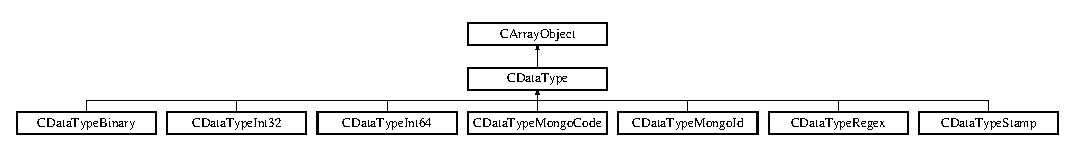
\includegraphics[height=1.578947cm]{class_c_data_type}
\end{center}
\end{figure}
\subsection*{Public Member Functions}
\begin{DoxyCompactItemize}
\item 
\hyperlink{class_c_data_type_a52f7a2ebe5e01eed9995115a410d83ab}{\-\_\-\-\_\-construct} (\$the\-Data=N\-U\-L\-L)
\item 
\hyperlink{class_c_data_type_a47c70c056d328f35497a6e712bf9be1c}{\-\_\-\-\_\-to\-String} ()
\item 
\hyperlink{class_c_data_type_a6f013843044529b54c2df535fc1471a8}{value} ()
\end{DoxyCompactItemize}
\subsection*{Static Public Member Functions}
\begin{DoxyCompactItemize}
\item 
static \hyperlink{class_c_data_type_a608d6fc184bce537ce83669f729d6008}{Serialise\-Object} (\&\$the\-Object)
\item 
static \hyperlink{class_c_data_type_ae15089a7237ed4e95279b398f44f8f47}{Serialise\-Element} (\&\$the\-Element, \&\$the\-Type)
\item 
static \hyperlink{class_c_data_type_a1cae522eec386d293b6087a99e9a8b0b}{Serialise\-Data} (\&\$the\-Element)
\end{DoxyCompactItemize}


\subsection{Constructor \& Destructor Documentation}
\hypertarget{class_c_data_type_a52f7a2ebe5e01eed9995115a410d83ab}{\index{C\-Data\-Type@{C\-Data\-Type}!\-\_\-\-\_\-construct@{\-\_\-\-\_\-construct}}
\index{\-\_\-\-\_\-construct@{\-\_\-\-\_\-construct}!CDataType@{C\-Data\-Type}}
\subsubsection[{\-\_\-\-\_\-construct}]{\setlength{\rightskip}{0pt plus 5cm}C\-Data\-Type\-::\-\_\-\-\_\-construct (
\begin{DoxyParamCaption}
\item[{}]{\$the\-Data = {\ttfamily NULL}}
\end{DoxyParamCaption}
)}}\label{class_c_data_type_a52f7a2ebe5e01eed9995115a410d83ab}
Instantiate class.

This class enforces a standard constructor that accepts one parameter which represents the custom data contents, these will be stored in the \hyperlink{}{k\-T\-A\-G\-\_\-\-D\-A\-T\-A} offset, this element must be filled.

The method will ensure that this parameter is not {\itshape N\-U\-L\-L} and not an array; it may be an Array\-Object, but it must then have the \-\_\-to\-String() method.

No {\itshape N\-U\-L\-L} concrete instance is allowed, all instances derived from this class must have a value.

The \hyperlink{}{k\-T\-A\-G\-\_\-\-T\-Y\-P\-E\} offset will be set by derived classes.  mixed \$the\-Data Custom data.  public  Exception }

Reimplemented in \hyperlink{class_c_data_type_stamp_a4ae6aac8e317e97afcf82bcd61450f52}{C\-Data\-Type\-Stamp}, \hyperlink{class_c_data_type_binary_a59d483e75d2facb20e958394039f6bf2}{C\-Data\-Type\-Binary}, \hyperlink{class_c_data_type_int64_ac628704dd037bbbc85601b4b111ea839}{C\-Data\-Type\-Int64}, \hyperlink{class_c_data_type_int32_a1181cc130ff3b0c573aeead09696b81f}{C\-Data\-Type\-Int32}, \hyperlink{class_c_data_type_mongo_code_a7eb2c6590e0a7ba7e5080a0953779786}{C\-Data\-Type\-Mongo\-Code}, \hyperlink{class_c_data_type_regex_a128da2b94c0b1a72fa44e656923e96d0}{C\-Data\-Type\-Regex}, and \hyperlink{class_c_data_type_mongo_id_a74cbfbb617dfdba49779b4392d01ccb2}{C\-Data\-Type\-Mongo\-Id}.



\subsection{Member Function Documentation}
\hypertarget{class_c_data_type_a47c70c056d328f35497a6e712bf9be1c}{\index{C\-Data\-Type@{C\-Data\-Type}!\-\_\-\-\_\-to\-String@{\-\_\-\-\_\-to\-String}}
\index{\-\_\-\-\_\-to\-String@{\-\_\-\-\_\-to\-String}!CDataType@{C\-Data\-Type}}
\subsubsection[{\-\_\-\-\_\-to\-String}]{\setlength{\rightskip}{0pt plus 5cm}C\-Data\-Type\-::\-\_\-\-\_\-to\-String (
\begin{DoxyParamCaption}
{}
\end{DoxyParamCaption}
)}}\label{class_c_data_type_a47c70c056d328f35497a6e712bf9be1c}
Return string representation.

This method should return a string representation of the custom data type contents, this method must be implemented for all concrete classes.

By default this method expects the custom data part to be convertable to string, if this is not the case, overload this method.

public \begin{DoxyReturn}{Returns}
string 
\end{DoxyReturn}


Reimplemented in \hyperlink{class_c_data_type_stamp_ab0256098cc25df9b50cc765a093d2cef}{C\-Data\-Type\-Stamp}.

\hypertarget{class_c_data_type_a1cae522eec386d293b6087a99e9a8b0b}{\index{C\-Data\-Type@{C\-Data\-Type}!Serialise\-Data@{Serialise\-Data}}
\index{Serialise\-Data@{Serialise\-Data}!CDataType@{C\-Data\-Type}}
\subsubsection[{Serialise\-Data}]{\setlength{\rightskip}{0pt plus 5cm}static C\-Data\-Type\-::\-Serialise\-Data (
\begin{DoxyParamCaption}
\item[{\&}]{\$the\-Element}
\end{DoxyParamCaption}
)\hspace{0.3cm}{\ttfamily [static]}}}\label{class_c_data_type_a1cae522eec386d293b6087a99e9a8b0b}
Serialise provided data element.

This method can be used to convert custom data types to a standard format that can be serialised and transmitted through the network. This method is generally called by \hyperlink{class_c_data_type_a608d6fc184bce537ce83669f729d6008}{Serialise\-Object} which passes each scalar element as a reference to this method which should decide whether the provided element is to be converted or not.

This method will check if the provided parameter corresponds to a custom data type that needs to be converted, if so, it will convert it to an instance derived from this class.

The following data types will be converted\-:


\begin{DoxyItemize}
\item {\itshape Mongo\-Id}\-: We convert into a \hyperlink{class_c_data_type_mongo_id}{C\-Data\-Type\-Mongo\-Id} object. 
\item {\itshape Mongo\-Code}\-: We convert into a \hyperlink{class_c_data_type_mongo_code}{C\-Data\-Type\-Mongo\-Code} object. 
\item {\itshape Mongo\-Date}\-: We convert into a \hyperlink{class_c_data_type_stamp}{C\-Data\-Type\-Stamp} object. 
\item {\itshape Mongo\-Regex}\-: We convert into a \hyperlink{class_c_data_type_regex}{C\-Data\-Type\-Regex} object. 
\item {\itshape Mongo\-Bin\-Data}\-: We convert into a \hyperlink{class_c_data_type_binary}{C\-Data\-Type\-Binary} object. 
\item {\itshape Mongo\-Int32}\-: We convert into a \hyperlink{class_c_data_type_int32}{C\-Data\-Type\-Int32} object. 
\item {\itshape Mongo\-Int64}\-: We convert into a \hyperlink{class_c_data_type_int64}{C\-Data\-Type\-Int64} object. 
\end{DoxyItemize}


\begin{DoxyParams}[1]{Parameters}
reference & {\em \&\$the\-Element} & Element to encode. \\
\hline
\end{DoxyParams}
\hypertarget{class_c_data_type_ae15089a7237ed4e95279b398f44f8f47}{\index{C\-Data\-Type@{C\-Data\-Type}!Serialise\-Element@{Serialise\-Element}}
\index{Serialise\-Element@{Serialise\-Element}!CDataType@{C\-Data\-Type}}
\subsubsection[{Serialise\-Element}]{\setlength{\rightskip}{0pt plus 5cm}static C\-Data\-Type\-::\-Serialise\-Element (
\begin{DoxyParamCaption}
\item[{\&}]{\$the\-Element, }
\item[{\&}]{\$the\-Type}
\end{DoxyParamCaption}
)\hspace{0.3cm}{\ttfamily [static]}}}\label{class_c_data_type_ae15089a7237ed4e95279b398f44f8f47}
Serialise provided element.

This method can be used to enforce converting custom data types to a standard format that can be serialised and transmitted through the network. This method accepts two parameters\-: the data type and the value\-: depending on their combination, the method will convert in place the data and the type.


\begin{DoxyParams}[1]{Parameters}
reference & {\em \&\$the\-Element} & Element to encode. \\
\hline
string & {\em \&\$the\-Type} & Element data type. \\
\hline
\end{DoxyParams}
\hypertarget{class_c_data_type_a608d6fc184bce537ce83669f729d6008}{\index{C\-Data\-Type@{C\-Data\-Type}!Serialise\-Object@{Serialise\-Object}}
\index{Serialise\-Object@{Serialise\-Object}!CDataType@{C\-Data\-Type}}
\subsubsection[{Serialise\-Object}]{\setlength{\rightskip}{0pt plus 5cm}static C\-Data\-Type\-::\-Serialise\-Object (
\begin{DoxyParamCaption}
\item[{\&}]{\$the\-Object}
\end{DoxyParamCaption}
)\hspace{0.3cm}{\ttfamily [static]}}}\label{class_c_data_type_a608d6fc184bce537ce83669f729d6008}
Serialise provided object.

This method will take an object and convert all data elements that are compatible with one of the concrete classes derived from this one into a derived concrete instance.

This method is useful when encoding objects in a format suitable for being transmitted, or just after \hyperlink{class_c_persistent_object_a88b1f2b11d3d60e0b3d33d8b0649b68a}{committing} them to a persistent \hyperlink{class_c_container}{container}.

This method will ensure that the object contains data types compatible with P\-H\-P and this library; it will be the duty of persistent \hyperlink{class_c_container}{containers} to convert these structures into custom data types compatible with their storage engines.

The method will scan the provided data elements\-: array or Array\-Object elements will be recursed, scalar elements will be sent to the public \hyperlink{class_c_data_type_a1cae522eec386d293b6087a99e9a8b0b}{Serialise\-Data} method that will take care of performing the actual data conversion.

If an element of the provided structure is converted, it will {\itshape always} be an object derived from this class, and all conversions will be performed on the object itself, which means that you should expect the provided object to be modified.


\begin{DoxyParams}[1]{Parameters}
reference & {\em \&\$the\-Object} & Object to decode. \\
\hline
\end{DoxyParams}
\hypertarget{class_c_data_type_a6f013843044529b54c2df535fc1471a8}{\index{C\-Data\-Type@{C\-Data\-Type}!value@{value}}
\index{value@{value}!CDataType@{C\-Data\-Type}}
\subsubsection[{value}]{\setlength{\rightskip}{0pt plus 5cm}C\-Data\-Type\-::value (
\begin{DoxyParamCaption}
{}
\end{DoxyParamCaption}
)}}\label{class_c_data_type_a6f013843044529b54c2df535fc1471a8}
Return data value.

This method should return the custom data value in the closest type possible in P\-H\-P.

By default we return the string representation of the data, this is the last resort if the actual data type cannot be represented in P\-H\-P; derived classes that can be represented in P\-H\-P should overload this method.

public \begin{DoxyReturn}{Returns}
mixed
\end{DoxyReturn}

\begin{DoxyExceptions}{Exceptions}
{\em Exception} & \\
\hline
\end{DoxyExceptions}


Reimplemented in \hyperlink{class_c_data_type_stamp_ac44e6be53a7dd369c159c19a5d31056c}{C\-Data\-Type\-Stamp}, \hyperlink{class_c_data_type_int64_a628aa7443dc28e2a6aaef982877d3559}{C\-Data\-Type\-Int64}, \hyperlink{class_c_data_type_binary_af2d723e4b5f85b3ecae701841ef27470}{C\-Data\-Type\-Binary}, \hyperlink{class_c_data_type_int32_a5d95fb33639cb10a3cd54dde2b771f91}{C\-Data\-Type\-Int32}, \hyperlink{class_c_data_type_mongo_code_a2f0db89da0c74ad4cfb3b0826aaefb70}{C\-Data\-Type\-Mongo\-Code}, \hyperlink{class_c_data_type_mongo_id_a24bd5d314b38fcb049d6600de0f191df}{C\-Data\-Type\-Mongo\-Id}, and \hyperlink{class_c_data_type_regex_a957186494f3c0e621540b972f51f5ea0}{C\-Data\-Type\-Regex}.



The documentation for this class was generated from the following file\-:\begin{DoxyCompactItemize}
\item 
/\-Library/\-Web\-Server/\-Library/wrapper/classes/C\-Data\-Type.\-php\end{DoxyCompactItemize}

\hypertarget{class_c_data_type_binary}{\section{C\-Data\-Type\-Binary Class Reference}
\label{class_c_data_type_binary}\index{C\-Data\-Type\-Binary@{C\-Data\-Type\-Binary}}
}
Inheritance diagram for C\-Data\-Type\-Binary\-:\begin{figure}[H]
\begin{center}
\leavevmode
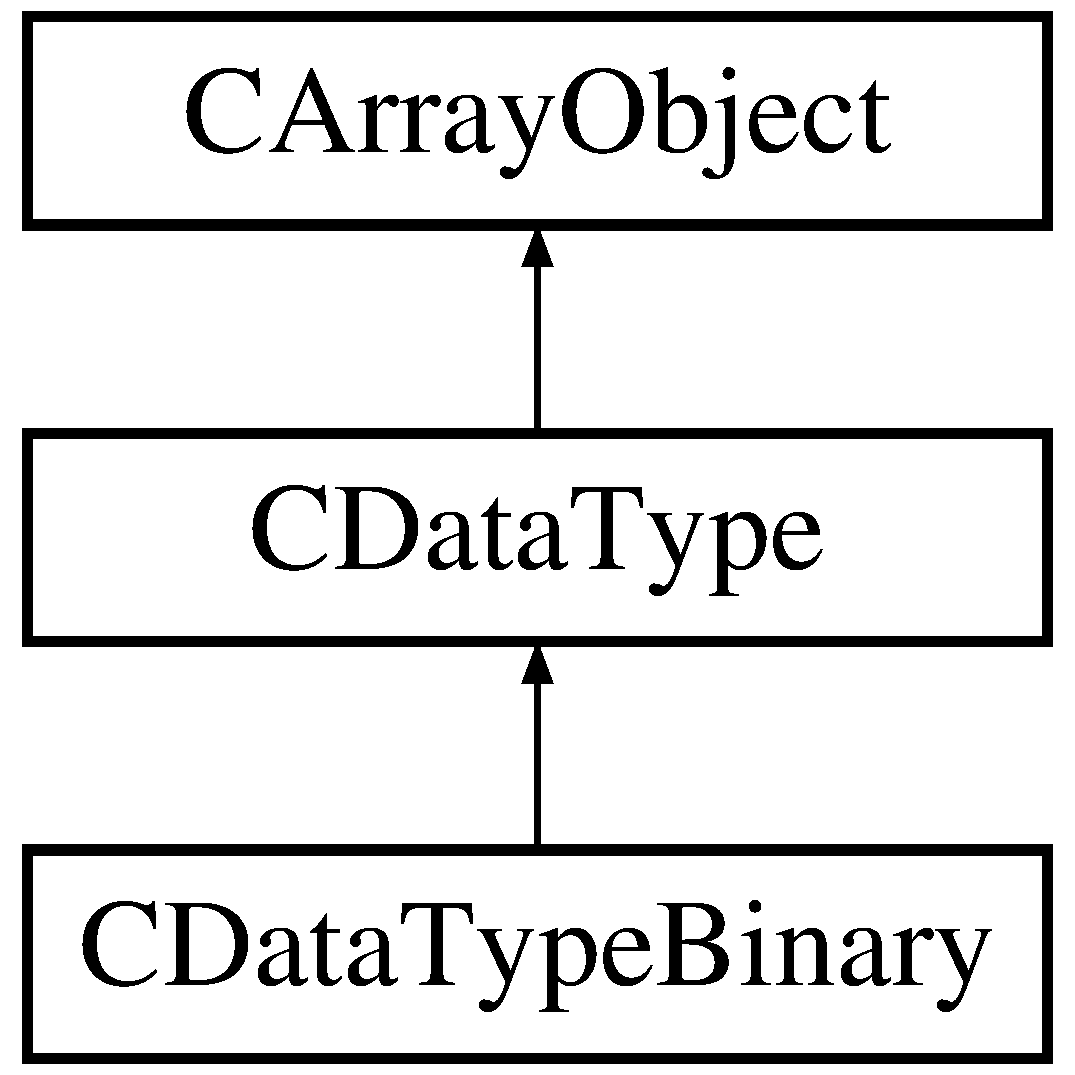
\includegraphics[height=3.000000cm]{class_c_data_type_binary}
\end{center}
\end{figure}
\subsection*{Public Member Functions}
\begin{DoxyCompactItemize}
\item 
\hyperlink{class_c_data_type_binary_a59d483e75d2facb20e958394039f6bf2}{\-\_\-\-\_\-construct} (\$the\-Data=N\-U\-L\-L)
\item 
\hyperlink{class_c_data_type_binary_af2d723e4b5f85b3ecae701841ef27470}{value} ()
\end{DoxyCompactItemize}
\subsection*{Additional Inherited Members}


\subsection{Constructor \& Destructor Documentation}
\hypertarget{class_c_data_type_binary_a59d483e75d2facb20e958394039f6bf2}{\index{C\-Data\-Type\-Binary@{C\-Data\-Type\-Binary}!\-\_\-\-\_\-construct@{\-\_\-\-\_\-construct}}
\index{\-\_\-\-\_\-construct@{\-\_\-\-\_\-construct}!CDataTypeBinary@{C\-Data\-Type\-Binary}}
\subsubsection[{\-\_\-\-\_\-construct}]{\setlength{\rightskip}{0pt plus 5cm}C\-Data\-Type\-Binary\-::\-\_\-\-\_\-construct (
\begin{DoxyParamCaption}
\item[{}]{\$the\-Data = {\ttfamily NULL}}
\end{DoxyParamCaption}
)}}\label{class_c_data_type_binary_a59d483e75d2facb20e958394039f6bf2}
Instantiate class.

We overload the parent constructor to set the default \hyperlink{}{offset} and to set the binary string into the \hyperlink{}{k\-T\-A\-G\-\_\-\-D\-A\-T\-A} offset.


\begin{DoxyParams}[1]{Parameters}
mixed & {\em \$the\-Data} & Custom data.\\
\hline
\end{DoxyParams}
public


\begin{DoxyExceptions}{Exceptions}
{\em Exception} & \\
\hline
\end{DoxyExceptions}


Reimplemented from \hyperlink{class_c_data_type_a52f7a2ebe5e01eed9995115a410d83ab}{C\-Data\-Type}.



\subsection{Member Function Documentation}
\hypertarget{class_c_data_type_binary_af2d723e4b5f85b3ecae701841ef27470}{\index{C\-Data\-Type\-Binary@{C\-Data\-Type\-Binary}!value@{value}}
\index{value@{value}!CDataTypeBinary@{C\-Data\-Type\-Binary}}
\subsubsection[{value}]{\setlength{\rightskip}{0pt plus 5cm}C\-Data\-Type\-Binary\-::value (
\begin{DoxyParamCaption}
{}
\end{DoxyParamCaption}
)}}\label{class_c_data_type_binary_af2d723e4b5f85b3ecae701841ef27470}
Return data value.

This method will return the actual binary string.

public \begin{DoxyReturn}{Returns}
float
\end{DoxyReturn}

\begin{DoxyExceptions}{Exceptions}
{\em Exception} & \\
\hline
\end{DoxyExceptions}


Reimplemented from \hyperlink{class_c_data_type_a6f013843044529b54c2df535fc1471a8}{C\-Data\-Type}.



The documentation for this class was generated from the following file\-:\begin{DoxyCompactItemize}
\item 
/\-Library/\-Web\-Server/\-Library/wrapper/classes/C\-Data\-Type\-Binary.\-php\end{DoxyCompactItemize}

\hypertarget{class_c_data_type_int32}{\section{C\-Data\-Type\-Int32 Class Reference}
\label{class_c_data_type_int32}\index{C\-Data\-Type\-Int32@{C\-Data\-Type\-Int32}}
}
Inheritance diagram for C\-Data\-Type\-Int32\-:\begin{figure}[H]
\begin{center}
\leavevmode
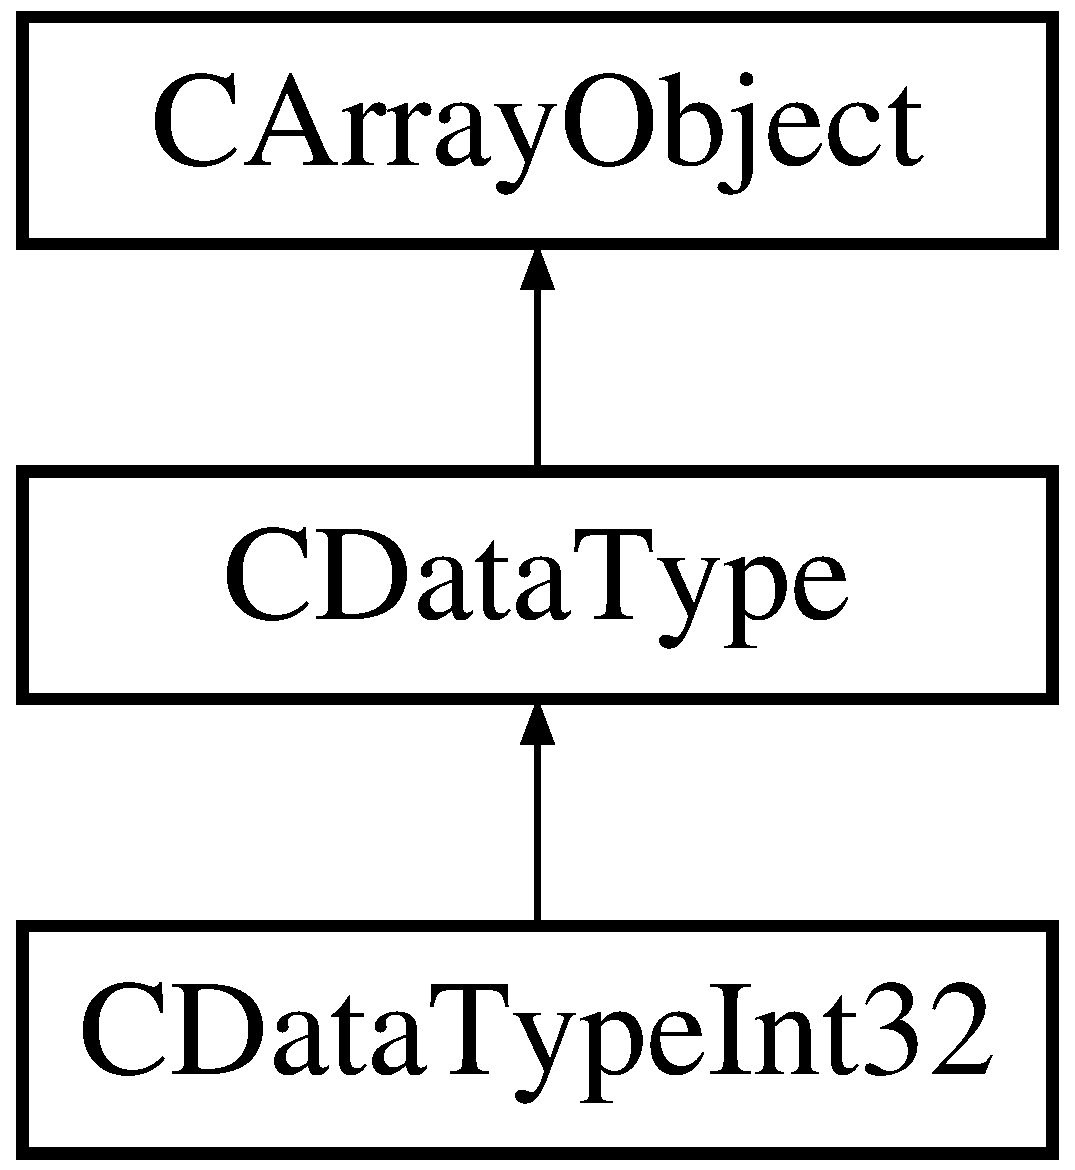
\includegraphics[height=3.000000cm]{class_c_data_type_int32}
\end{center}
\end{figure}
\subsection*{Public Member Functions}
\begin{DoxyCompactItemize}
\item 
\hyperlink{class_c_data_type_int32_a1181cc130ff3b0c573aeead09696b81f}{\-\_\-\-\_\-construct} (\$the\-Data=N\-U\-L\-L)
\item 
\hyperlink{class_c_data_type_int32_a5d95fb33639cb10a3cd54dde2b771f91}{value} ()
\end{DoxyCompactItemize}
\subsection*{Additional Inherited Members}


\subsection{Constructor \& Destructor Documentation}
\hypertarget{class_c_data_type_int32_a1181cc130ff3b0c573aeead09696b81f}{\index{C\-Data\-Type\-Int32@{C\-Data\-Type\-Int32}!\-\_\-\-\_\-construct@{\-\_\-\-\_\-construct}}
\index{\-\_\-\-\_\-construct@{\-\_\-\-\_\-construct}!CDataTypeInt32@{C\-Data\-Type\-Int32}}
\subsubsection[{\-\_\-\-\_\-construct}]{\setlength{\rightskip}{0pt plus 5cm}C\-Data\-Type\-Int32\-::\-\_\-\-\_\-construct (
\begin{DoxyParamCaption}
\item[{}]{\$the\-Data = {\ttfamily NULL}}
\end{DoxyParamCaption}
)}}\label{class_c_data_type_int32_a1181cc130ff3b0c573aeead09696b81f}
Instantiate class.

In this class we store \hyperlink{}{k\-T\-Y\-P\-E\-\_\-\-I\-N\-T32} in the \hyperlink{}{k\-T\-A\-G\-\_\-\-T\-Y\-P\-E} offset and the integer in the \hyperlink{}{k\-T\-A\-G\-\_\-\-D\-A\-T\-A} offset.

The method will check if the provided data (converted to string) is numeric, if this is not the case, it will raise an exception. This is to handle miscellaneous objects.


\begin{DoxyParams}[1]{Parameters}
mixed & {\em \$the\-Data} & Custom data.\\
\hline
\end{DoxyParams}
public


\begin{DoxyExceptions}{Exceptions}
{\em Exception} & \\
\hline
\end{DoxyExceptions}


Reimplemented from \hyperlink{class_c_data_type_a52f7a2ebe5e01eed9995115a410d83ab}{C\-Data\-Type}.



\subsection{Member Function Documentation}
\hypertarget{class_c_data_type_int32_a5d95fb33639cb10a3cd54dde2b771f91}{\index{C\-Data\-Type\-Int32@{C\-Data\-Type\-Int32}!value@{value}}
\index{value@{value}!CDataTypeInt32@{C\-Data\-Type\-Int32}}
\subsubsection[{value}]{\setlength{\rightskip}{0pt plus 5cm}C\-Data\-Type\-Int32\-::value (
\begin{DoxyParamCaption}
{}
\end{DoxyParamCaption}
)}}\label{class_c_data_type_int32_a5d95fb33639cb10a3cd54dde2b771f91}
Return data value.

In this class we return the integer value, since P\-H\-P handles it.

public \begin{DoxyReturn}{Returns}
mixed
\end{DoxyReturn}

\begin{DoxyExceptions}{Exceptions}
{\em Exception} & \\
\hline
\end{DoxyExceptions}


Reimplemented from \hyperlink{class_c_data_type_a6f013843044529b54c2df535fc1471a8}{C\-Data\-Type}.



The documentation for this class was generated from the following file\-:\begin{DoxyCompactItemize}
\item 
/\-Library/\-Web\-Server/\-Library/wrapper/classes/C\-Data\-Type\-Int32.\-php\end{DoxyCompactItemize}

\hypertarget{class_c_data_type_int64}{\section{C\-Data\-Type\-Int64 Class Reference}
\label{class_c_data_type_int64}\index{C\-Data\-Type\-Int64@{C\-Data\-Type\-Int64}}
}
Inheritance diagram for C\-Data\-Type\-Int64\-:\begin{figure}[H]
\begin{center}
\leavevmode
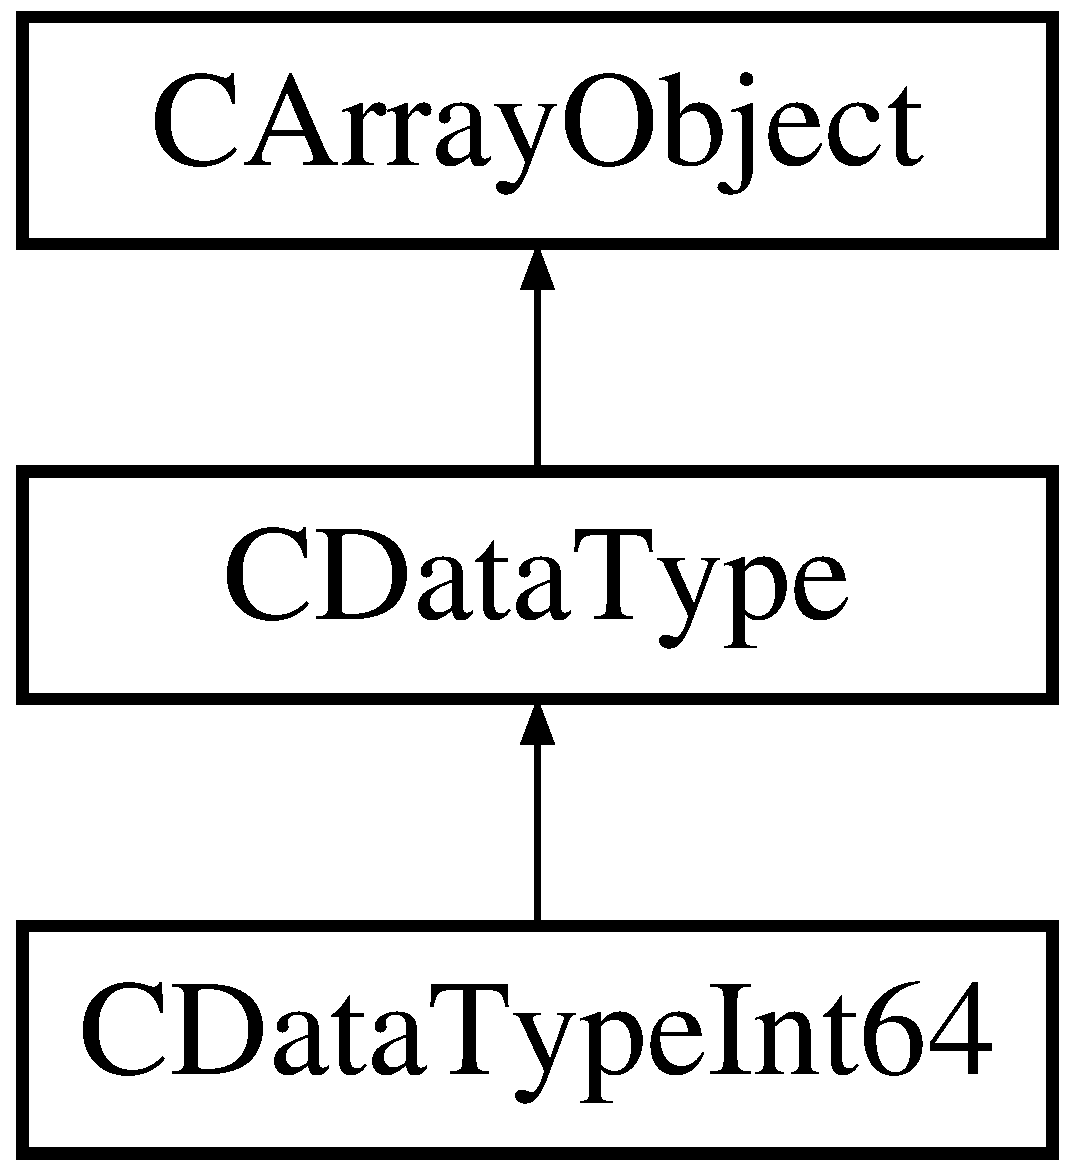
\includegraphics[height=3.000000cm]{class_c_data_type_int64}
\end{center}
\end{figure}
\subsection*{Public Member Functions}
\begin{DoxyCompactItemize}
\item 
\hyperlink{class_c_data_type_int64_ac628704dd037bbbc85601b4b111ea839}{\-\_\-\-\_\-construct} (\$the\-Data=N\-U\-L\-L)
\item 
\hyperlink{class_c_data_type_int64_a628aa7443dc28e2a6aaef982877d3559}{value} ()
\end{DoxyCompactItemize}
\subsection*{Additional Inherited Members}


\subsection{Constructor \& Destructor Documentation}
\hypertarget{class_c_data_type_int64_ac628704dd037bbbc85601b4b111ea839}{\index{C\-Data\-Type\-Int64@{C\-Data\-Type\-Int64}!\-\_\-\-\_\-construct@{\-\_\-\-\_\-construct}}
\index{\-\_\-\-\_\-construct@{\-\_\-\-\_\-construct}!CDataTypeInt64@{C\-Data\-Type\-Int64}}
\subsubsection[{\-\_\-\-\_\-construct}]{\setlength{\rightskip}{0pt plus 5cm}C\-Data\-Type\-Int64\-::\-\_\-\-\_\-construct (
\begin{DoxyParamCaption}
\item[{}]{\$the\-Data = {\ttfamily NULL}}
\end{DoxyParamCaption}
)}}\label{class_c_data_type_int64_ac628704dd037bbbc85601b4b111ea839}
Instantiate class.

In this class we store \hyperlink{}{k\-T\-Y\-P\-E\-\_\-\-I\-N\-T64} in the \hyperlink{}{k\-T\-A\-G\-\_\-\-T\-Y\-P\-E} offset and the integer in the \hyperlink{}{k\-T\-A\-G\-\_\-\-D\-A\-T\-A} offset.

The method will check if the provided data (converted to string) is numeric, if this is not the case, it will raise an exception. This is to handle miscellaneous objects.

The number will be stored in the \hyperlink{}{k\-T\-A\-G\-\_\-\-D\-A\-T\-A} offset as an integer, if the current system is 64 bits.


\begin{DoxyParams}[1]{Parameters}
mixed & {\em \$the\-Data} & Custom data.\\
\hline
\end{DoxyParams}
public


\begin{DoxyExceptions}{Exceptions}
{\em Exception} & \\
\hline
\end{DoxyExceptions}


Reimplemented from \hyperlink{class_c_data_type_a52f7a2ebe5e01eed9995115a410d83ab}{C\-Data\-Type}.



\subsection{Member Function Documentation}
\hypertarget{class_c_data_type_int64_a628aa7443dc28e2a6aaef982877d3559}{\index{C\-Data\-Type\-Int64@{C\-Data\-Type\-Int64}!value@{value}}
\index{value@{value}!CDataTypeInt64@{C\-Data\-Type\-Int64}}
\subsubsection[{value}]{\setlength{\rightskip}{0pt plus 5cm}C\-Data\-Type\-Int64\-::value (
\begin{DoxyParamCaption}
{}
\end{DoxyParamCaption}
)}}\label{class_c_data_type_int64_a628aa7443dc28e2a6aaef982877d3559}
Return data value.

In this class we return the integer value, if P\-H\-P handles 8 byte integers, or we call the \hyperlink{class_c_data_type_a6f013843044529b54c2df535fc1471a8}{parent} method.

public \begin{DoxyReturn}{Returns}
mixed
\end{DoxyReturn}

\begin{DoxyExceptions}{Exceptions}
{\em Exception} & \\
\hline
\end{DoxyExceptions}


Reimplemented from \hyperlink{class_c_data_type_a6f013843044529b54c2df535fc1471a8}{C\-Data\-Type}.



The documentation for this class was generated from the following file\-:\begin{DoxyCompactItemize}
\item 
/\-Library/\-Web\-Server/\-Library/wrapper/classes/C\-Data\-Type\-Int64.\-php\end{DoxyCompactItemize}

\hypertarget{class_c_data_type_mongo_code}{\section{C\-Data\-Type\-Mongo\-Code Class Reference}
\label{class_c_data_type_mongo_code}\index{C\-Data\-Type\-Mongo\-Code@{C\-Data\-Type\-Mongo\-Code}}
}
Inheritance diagram for C\-Data\-Type\-Mongo\-Code\-:\begin{figure}[H]
\begin{center}
\leavevmode
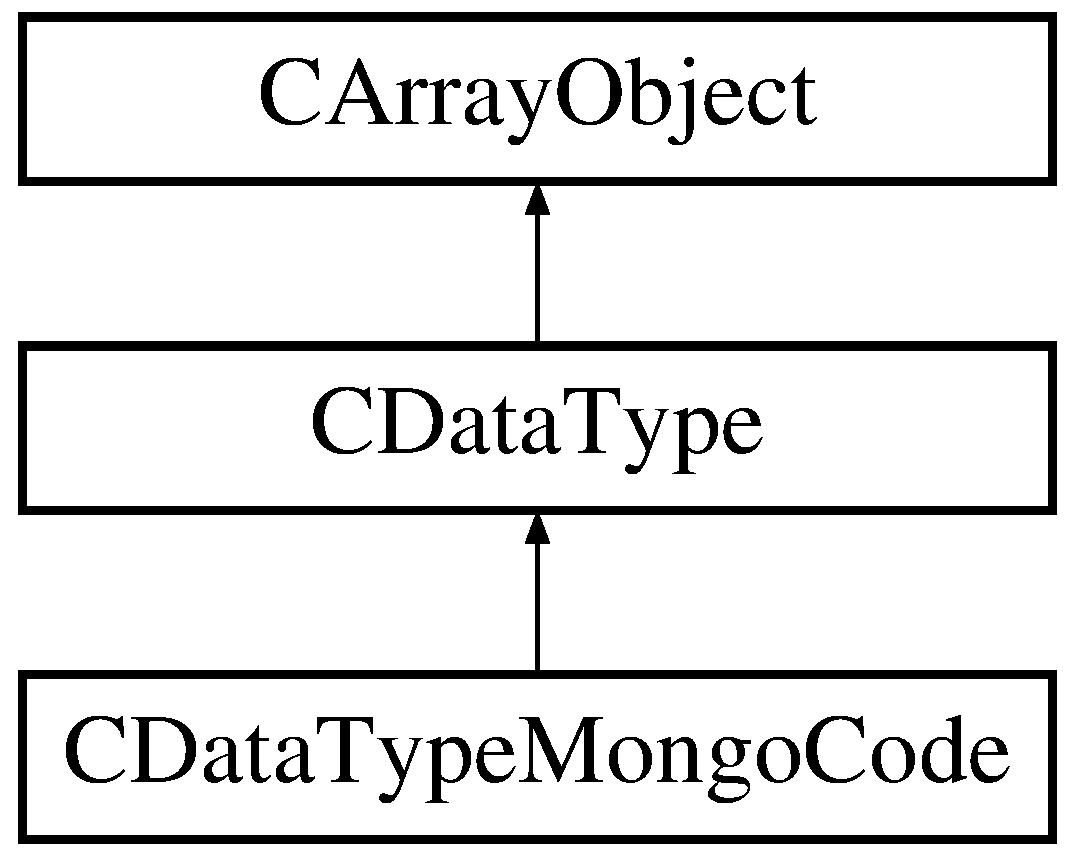
\includegraphics[height=3.000000cm]{class_c_data_type_mongo_code}
\end{center}
\end{figure}
\subsection*{Public Member Functions}
\begin{DoxyCompactItemize}
\item 
\hyperlink{class_c_data_type_mongo_code_a7eb2c6590e0a7ba7e5080a0953779786}{\-\_\-\-\_\-construct} (\$the\-Data=N\-U\-L\-L)
\item 
\hyperlink{class_c_data_type_mongo_code_a2f0db89da0c74ad4cfb3b0826aaefb70}{value} ()
\end{DoxyCompactItemize}
\subsection*{Additional Inherited Members}


\subsection{Constructor \& Destructor Documentation}
\hypertarget{class_c_data_type_mongo_code_a7eb2c6590e0a7ba7e5080a0953779786}{\index{C\-Data\-Type\-Mongo\-Code@{C\-Data\-Type\-Mongo\-Code}!\-\_\-\-\_\-construct@{\-\_\-\-\_\-construct}}
\index{\-\_\-\-\_\-construct@{\-\_\-\-\_\-construct}!CDataTypeMongoCode@{C\-Data\-Type\-Mongo\-Code}}
\subsubsection[{\-\_\-\-\_\-construct}]{\setlength{\rightskip}{0pt plus 5cm}C\-Data\-Type\-Mongo\-Code\-::\-\_\-\-\_\-construct (
\begin{DoxyParamCaption}
\item[{}]{\$the\-Data = {\ttfamily NULL}}
\end{DoxyParamCaption}
)}}\label{class_c_data_type_mongo_code_a7eb2c6590e0a7ba7e5080a0953779786}
Instantiate class.

In this class we can only instantiate such an object from a Mongo\-Code object.


\begin{DoxyParams}[1]{Parameters}
mixed & {\em \$the\-Data} & Custom data.\\
\hline
\end{DoxyParams}
public


\begin{DoxyExceptions}{Exceptions}
{\em Exception} & \\
\hline
\end{DoxyExceptions}


Reimplemented from \hyperlink{class_c_data_type_a52f7a2ebe5e01eed9995115a410d83ab}{C\-Data\-Type}.



\subsection{Member Function Documentation}
\hypertarget{class_c_data_type_mongo_code_a2f0db89da0c74ad4cfb3b0826aaefb70}{\index{C\-Data\-Type\-Mongo\-Code@{C\-Data\-Type\-Mongo\-Code}!value@{value}}
\index{value@{value}!CDataTypeMongoCode@{C\-Data\-Type\-Mongo\-Code}}
\subsubsection[{value}]{\setlength{\rightskip}{0pt plus 5cm}C\-Data\-Type\-Mongo\-Code\-::value (
\begin{DoxyParamCaption}
{}
\end{DoxyParamCaption}
)}}\label{class_c_data_type_mongo_code_a2f0db89da0c74ad4cfb3b0826aaefb70}
Return data value.

In this class we return the Mongo\-Code object.

public \begin{DoxyReturn}{Returns}
mixed
\end{DoxyReturn}

\begin{DoxyExceptions}{Exceptions}
{\em Exception} & \\
\hline
\end{DoxyExceptions}


Reimplemented from \hyperlink{class_c_data_type_a6f013843044529b54c2df535fc1471a8}{C\-Data\-Type}.



The documentation for this class was generated from the following file\-:\begin{DoxyCompactItemize}
\item 
/\-Library/\-Web\-Server/\-Library/wrapper/classes/C\-Data\-Type\-Mongo\-Code.\-php\end{DoxyCompactItemize}

\hypertarget{class_c_data_type_mongo_id}{\section{C\-Data\-Type\-Mongo\-Id Class Reference}
\label{class_c_data_type_mongo_id}\index{C\-Data\-Type\-Mongo\-Id@{C\-Data\-Type\-Mongo\-Id}}
}
Inheritance diagram for C\-Data\-Type\-Mongo\-Id\-:\begin{figure}[H]
\begin{center}
\leavevmode
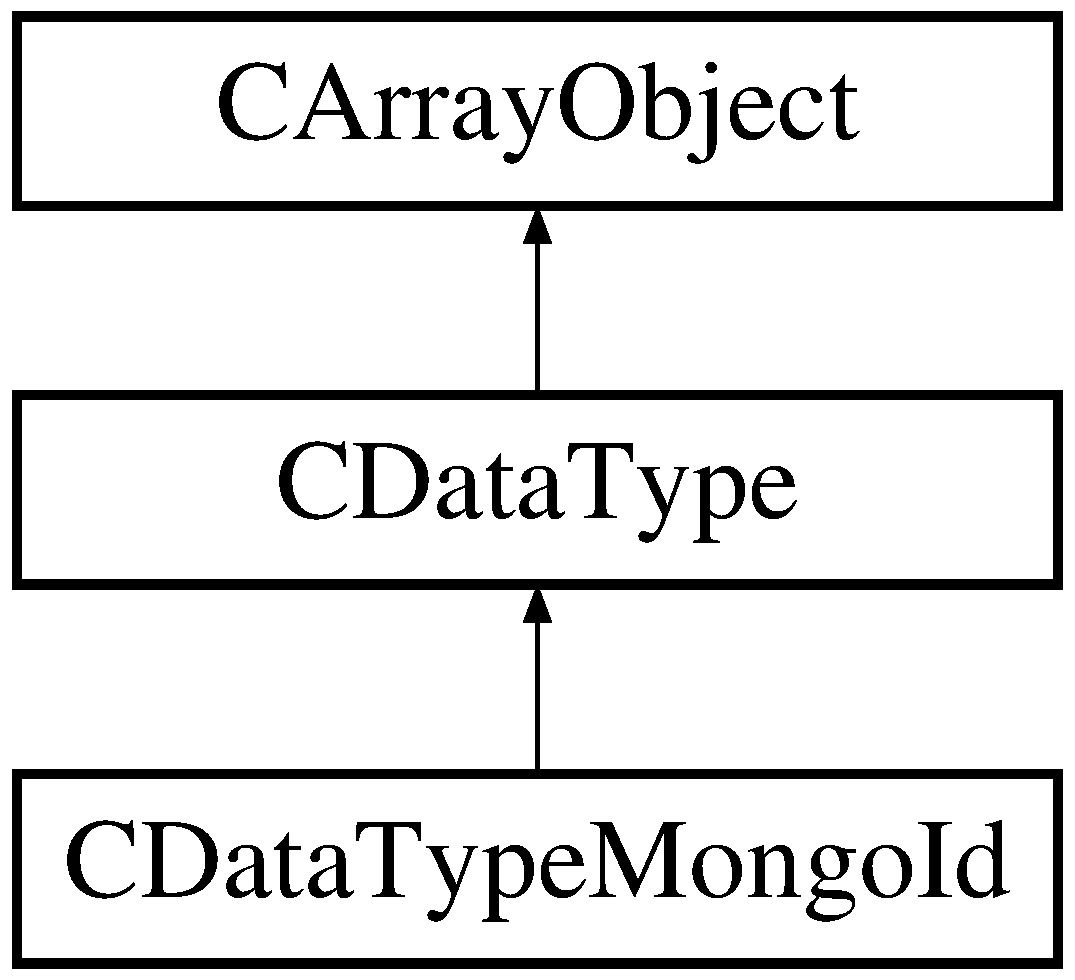
\includegraphics[height=3.000000cm]{class_c_data_type_mongo_id}
\end{center}
\end{figure}
\subsection*{Public Member Functions}
\begin{DoxyCompactItemize}
\item 
\hyperlink{class_c_data_type_mongo_id_a74cbfbb617dfdba49779b4392d01ccb2}{\-\_\-\-\_\-construct} (\$the\-Data=N\-U\-L\-L)
\item 
\hyperlink{class_c_data_type_mongo_id_a24bd5d314b38fcb049d6600de0f191df}{value} ()
\end{DoxyCompactItemize}
\subsection*{Additional Inherited Members}


\subsection{Constructor \& Destructor Documentation}
\hypertarget{class_c_data_type_mongo_id_a74cbfbb617dfdba49779b4392d01ccb2}{\index{C\-Data\-Type\-Mongo\-Id@{C\-Data\-Type\-Mongo\-Id}!\-\_\-\-\_\-construct@{\-\_\-\-\_\-construct}}
\index{\-\_\-\-\_\-construct@{\-\_\-\-\_\-construct}!CDataTypeMongoId@{C\-Data\-Type\-Mongo\-Id}}
\subsubsection[{\-\_\-\-\_\-construct}]{\setlength{\rightskip}{0pt plus 5cm}C\-Data\-Type\-Mongo\-Id\-::\-\_\-\-\_\-construct (
\begin{DoxyParamCaption}
\item[{}]{\$the\-Data = {\ttfamily NULL}}
\end{DoxyParamCaption}
)}}\label{class_c_data_type_mongo_id_a74cbfbb617dfdba49779b4392d01ccb2}
Instantiate class.

We overload the parent constructor to set the default \hyperlink{}{offset} and to set the H\-E\-X string into the \hyperlink{}{k\-T\-A\-G\-\_\-\-D\-A\-T\-A} offset.


\begin{DoxyParams}[1]{Parameters}
mixed & {\em \$the\-Data} & Custom data.\\
\hline
\end{DoxyParams}
public


\begin{DoxyExceptions}{Exceptions}
{\em Exception} & \\
\hline
\end{DoxyExceptions}


Reimplemented from \hyperlink{class_c_data_type_a52f7a2ebe5e01eed9995115a410d83ab}{C\-Data\-Type}.



\subsection{Member Function Documentation}
\hypertarget{class_c_data_type_mongo_id_a24bd5d314b38fcb049d6600de0f191df}{\index{C\-Data\-Type\-Mongo\-Id@{C\-Data\-Type\-Mongo\-Id}!value@{value}}
\index{value@{value}!CDataTypeMongoId@{C\-Data\-Type\-Mongo\-Id}}
\subsubsection[{value}]{\setlength{\rightskip}{0pt plus 5cm}C\-Data\-Type\-Mongo\-Id\-::value (
\begin{DoxyParamCaption}
{}
\end{DoxyParamCaption}
)}}\label{class_c_data_type_mongo_id_a24bd5d314b38fcb049d6600de0f191df}
Return data value.

In this class we return the Mongo\-Id object.

public \begin{DoxyReturn}{Returns}
mixed
\end{DoxyReturn}

\begin{DoxyExceptions}{Exceptions}
{\em Exception} & \\
\hline
\end{DoxyExceptions}


Reimplemented from \hyperlink{class_c_data_type_a6f013843044529b54c2df535fc1471a8}{C\-Data\-Type}.



The documentation for this class was generated from the following file\-:\begin{DoxyCompactItemize}
\item 
/\-Library/\-Web\-Server/\-Library/wrapper/classes/C\-Data\-Type\-Mongo\-Id.\-php\end{DoxyCompactItemize}

\hypertarget{class_c_data_type_regex}{\section{C\-Data\-Type\-Regex Class Reference}
\label{class_c_data_type_regex}\index{C\-Data\-Type\-Regex@{C\-Data\-Type\-Regex}}
}
Inheritance diagram for C\-Data\-Type\-Regex\-:\begin{figure}[H]
\begin{center}
\leavevmode
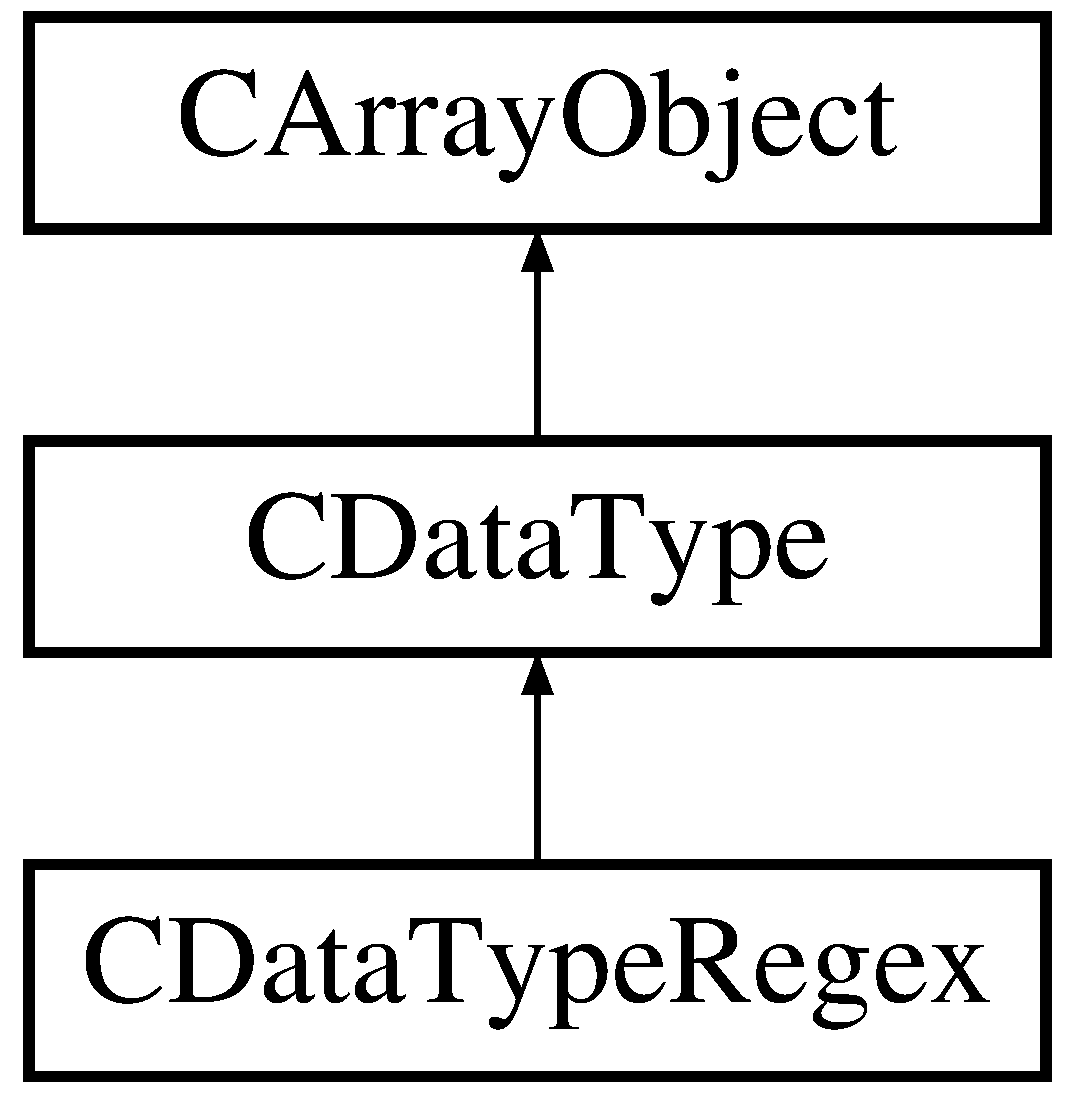
\includegraphics[height=3.000000cm]{class_c_data_type_regex}
\end{center}
\end{figure}
\subsection*{Public Member Functions}
\begin{DoxyCompactItemize}
\item 
\hyperlink{class_c_data_type_regex_a128da2b94c0b1a72fa44e656923e96d0}{\-\_\-\-\_\-construct} (\$the\-Data=N\-U\-L\-L)
\item 
\hyperlink{class_c_data_type_regex_a957186494f3c0e621540b972f51f5ea0}{value} ()
\end{DoxyCompactItemize}
\subsection*{Additional Inherited Members}


\subsection{Constructor \& Destructor Documentation}
\hypertarget{class_c_data_type_regex_a128da2b94c0b1a72fa44e656923e96d0}{\index{C\-Data\-Type\-Regex@{C\-Data\-Type\-Regex}!\-\_\-\-\_\-construct@{\-\_\-\-\_\-construct}}
\index{\-\_\-\-\_\-construct@{\-\_\-\-\_\-construct}!CDataTypeRegex@{C\-Data\-Type\-Regex}}
\subsubsection[{\-\_\-\-\_\-construct}]{\setlength{\rightskip}{0pt plus 5cm}C\-Data\-Type\-Regex\-::\-\_\-\-\_\-construct (
\begin{DoxyParamCaption}
\item[{}]{\$the\-Data = {\ttfamily NULL}}
\end{DoxyParamCaption}
)}}\label{class_c_data_type_regex_a128da2b94c0b1a72fa44e656923e96d0}
Instantiate class.

In this class we instantiate such an object from a Mongo\-Regex object or from a string.


\begin{DoxyParams}[1]{Parameters}
mixed & {\em \$the\-Data} & Custom data.\\
\hline
\end{DoxyParams}
public


\begin{DoxyExceptions}{Exceptions}
{\em Exception} & \\
\hline
\end{DoxyExceptions}


Reimplemented from \hyperlink{class_c_data_type_a52f7a2ebe5e01eed9995115a410d83ab}{C\-Data\-Type}.



\subsection{Member Function Documentation}
\hypertarget{class_c_data_type_regex_a957186494f3c0e621540b972f51f5ea0}{\index{C\-Data\-Type\-Regex@{C\-Data\-Type\-Regex}!value@{value}}
\index{value@{value}!CDataTypeRegex@{C\-Data\-Type\-Regex}}
\subsubsection[{value}]{\setlength{\rightskip}{0pt plus 5cm}C\-Data\-Type\-Regex\-::value (
\begin{DoxyParamCaption}
{}
\end{DoxyParamCaption}
)}}\label{class_c_data_type_regex_a957186494f3c0e621540b972f51f5ea0}
Return data value.

In this class we return the Mongo\-Regex object.

public \begin{DoxyReturn}{Returns}
mixed
\end{DoxyReturn}

\begin{DoxyExceptions}{Exceptions}
{\em Exception} & \\
\hline
\end{DoxyExceptions}


Reimplemented from \hyperlink{class_c_data_type_a6f013843044529b54c2df535fc1471a8}{C\-Data\-Type}.



The documentation for this class was generated from the following file\-:\begin{DoxyCompactItemize}
\item 
/\-Library/\-Web\-Server/\-Library/wrapper/classes/C\-Data\-Type\-Regex.\-php\end{DoxyCompactItemize}

\hypertarget{class_c_data_type_stamp}{\section{C\-Data\-Type\-Stamp Class Reference}
\label{class_c_data_type_stamp}\index{C\-Data\-Type\-Stamp@{C\-Data\-Type\-Stamp}}
}
Inheritance diagram for C\-Data\-Type\-Stamp\-:\begin{figure}[H]
\begin{center}
\leavevmode
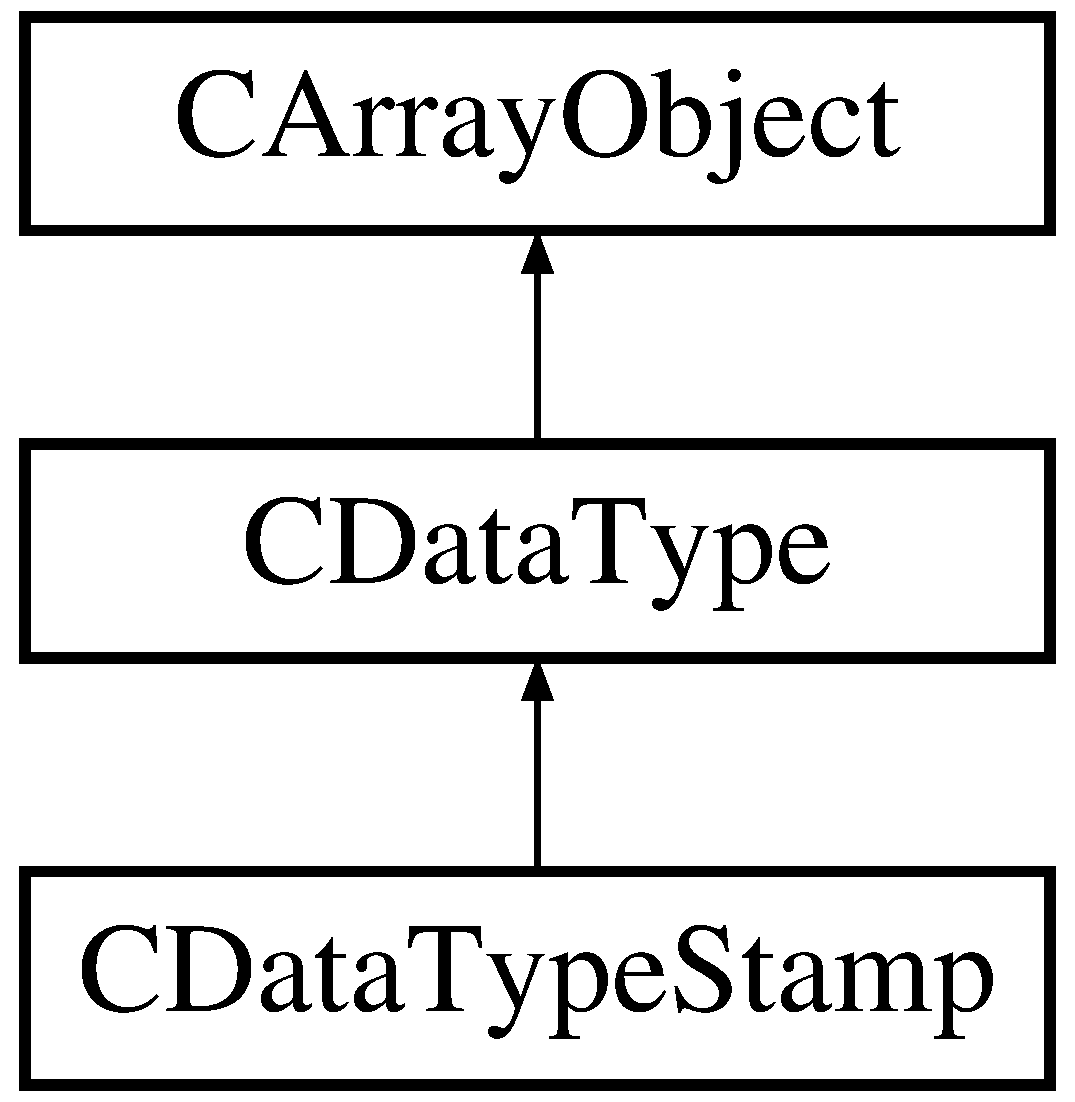
\includegraphics[height=3.000000cm]{class_c_data_type_stamp}
\end{center}
\end{figure}
\subsection*{Public Member Functions}
\begin{DoxyCompactItemize}
\item 
\hyperlink{class_c_data_type_stamp_a4ae6aac8e317e97afcf82bcd61450f52}{\-\_\-\-\_\-construct} (\$the\-Data=N\-U\-L\-L)
\item 
\hyperlink{class_c_data_type_stamp_ab0256098cc25df9b50cc765a093d2cef}{\-\_\-\-\_\-to\-String} ()
\item 
\hyperlink{class_c_data_type_stamp_ac44e6be53a7dd369c159c19a5d31056c}{value} ()
\end{DoxyCompactItemize}
\subsection*{Additional Inherited Members}


\subsection{Constructor \& Destructor Documentation}
\hypertarget{class_c_data_type_stamp_a4ae6aac8e317e97afcf82bcd61450f52}{\index{C\-Data\-Type\-Stamp@{C\-Data\-Type\-Stamp}!\-\_\-\-\_\-construct@{\-\_\-\-\_\-construct}}
\index{\-\_\-\-\_\-construct@{\-\_\-\-\_\-construct}!CDataTypeStamp@{C\-Data\-Type\-Stamp}}
\subsubsection[{\-\_\-\-\_\-construct}]{\setlength{\rightskip}{0pt plus 5cm}C\-Data\-Type\-Stamp\-::\-\_\-\-\_\-construct (
\begin{DoxyParamCaption}
\item[{}]{\$the\-Data = {\ttfamily NULL}}
\end{DoxyParamCaption}
)}}\label{class_c_data_type_stamp_a4ae6aac8e317e97afcf82bcd61450f52}
Instantiate class.

We overload the parent constructor to handle different types of data\-:


\begin{DoxyItemize}
\item {\itshape float}\-: If the data is a float, we assume it is the result of {\itshape microtime( T\-R\-U\-E )} in which the integral part of the number represents the number of seconds since January 1st 1970 G\-M\-T, and the fractional part represents the microseconds. 
\item {\itshape integer}\-: If the data is an integer, we assume it represents the number of seconds since January 1st 1970 G\-M\-T. 
\item {\itshape Mongo\-Date}\-: We use the object's elements. 
\item {\itshape Date\-Time}\-: We get the date seconds count. 
\item {\itshape other}\-: We assume the data is a date time string. 
\end{DoxyItemize}

No {\itshape N\-U\-L\-L} concrete instance is allowed, all instances derived from this class must have a value.


\begin{DoxyParams}[1]{Parameters}
mixed & {\em \$the\-Data} & Custom data.\\
\hline
\end{DoxyParams}
public


\begin{DoxyExceptions}{Exceptions}
{\em Exception} & \\
\hline
\end{DoxyExceptions}


Reimplemented from \hyperlink{class_c_data_type_a52f7a2ebe5e01eed9995115a410d83ab}{C\-Data\-Type}.



\subsection{Member Function Documentation}
\hypertarget{class_c_data_type_stamp_ab0256098cc25df9b50cc765a093d2cef}{\index{C\-Data\-Type\-Stamp@{C\-Data\-Type\-Stamp}!\-\_\-\-\_\-to\-String@{\-\_\-\-\_\-to\-String}}
\index{\-\_\-\-\_\-to\-String@{\-\_\-\-\_\-to\-String}!CDataTypeStamp@{C\-Data\-Type\-Stamp}}
\subsubsection[{\-\_\-\-\_\-to\-String}]{\setlength{\rightskip}{0pt plus 5cm}C\-Data\-Type\-Stamp\-::\-\_\-\-\_\-to\-String (
\begin{DoxyParamCaption}
{}
\end{DoxyParamCaption}
)}}\label{class_c_data_type_stamp_ab0256098cc25df9b50cc765a093d2cef}
Return string representation.

This method should return a string representation of the custom data type contents, this method must be implemented for all concrete classes.

By default this method expects the custom data part to be convertable to string, if this is not the case, overload this method.

public \begin{DoxyReturn}{Returns}
string 
\end{DoxyReturn}


Reimplemented from \hyperlink{class_c_data_type_a47c70c056d328f35497a6e712bf9be1c}{C\-Data\-Type}.

\hypertarget{class_c_data_type_stamp_ac44e6be53a7dd369c159c19a5d31056c}{\index{C\-Data\-Type\-Stamp@{C\-Data\-Type\-Stamp}!value@{value}}
\index{value@{value}!CDataTypeStamp@{C\-Data\-Type\-Stamp}}
\subsubsection[{value}]{\setlength{\rightskip}{0pt plus 5cm}C\-Data\-Type\-Stamp\-::value (
\begin{DoxyParamCaption}
{}
\end{DoxyParamCaption}
)}}\label{class_c_data_type_stamp_ac44e6be53a7dd369c159c19a5d31056c}
Return data value.

This method will return a floating point number equivalent to the result of the {\itshape microtime( T\-R\-U\-E )} function.

public \begin{DoxyReturn}{Returns}
float
\end{DoxyReturn}

\begin{DoxyExceptions}{Exceptions}
{\em Exception} & \\
\hline
\end{DoxyExceptions}


Reimplemented from \hyperlink{class_c_data_type_a6f013843044529b54c2df535fc1471a8}{C\-Data\-Type}.



The documentation for this class was generated from the following file\-:\begin{DoxyCompactItemize}
\item 
/\-Library/\-Web\-Server/\-Library/wrapper/classes/C\-Data\-Type\-Stamp.\-php\end{DoxyCompactItemize}

\hypertarget{class_c_data_wrapper}{\section{C\-Data\-Wrapper Class Reference}
\label{class_c_data_wrapper}\index{C\-Data\-Wrapper@{C\-Data\-Wrapper}}
}
Inheritance diagram for C\-Data\-Wrapper\-:\begin{figure}[H]
\begin{center}
\leavevmode
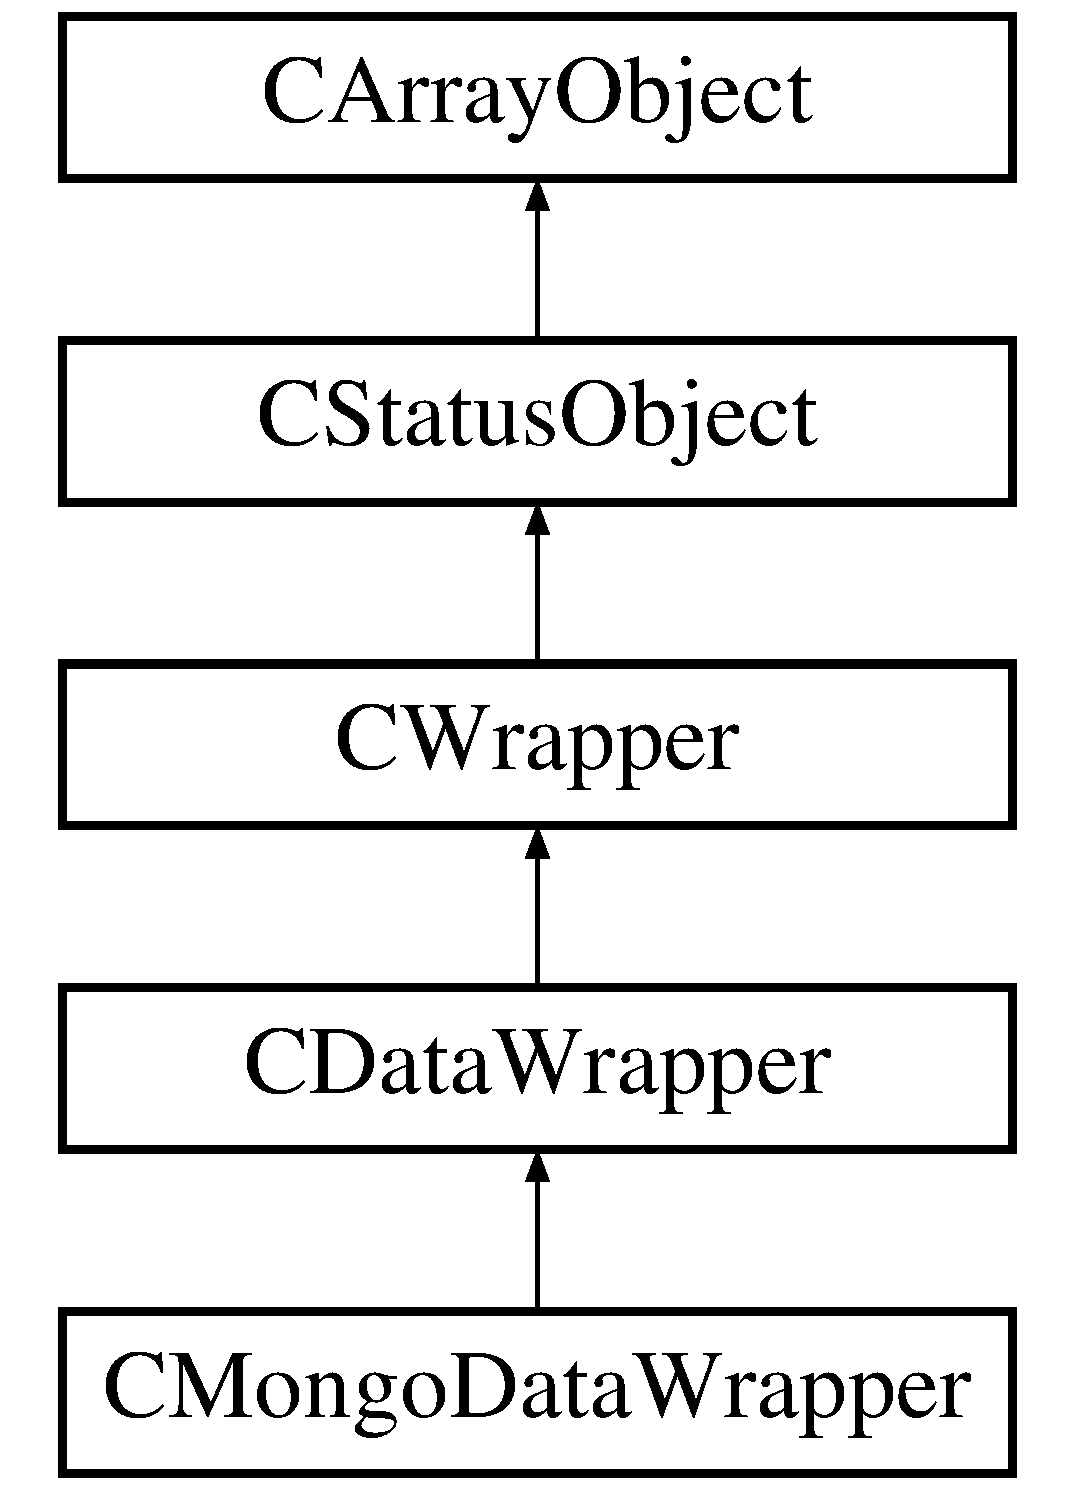
\includegraphics[height=5.000000cm]{class_c_data_wrapper}
\end{center}
\end{figure}
\subsection*{Protected Member Functions}
\begin{DoxyCompactItemize}
\item 
\hyperlink{class_c_data_wrapper_a85c97add738d08f2f2a9958ffbda6c03}{\-\_\-\-Init\-Options} ()
\item 
\hyperlink{class_c_data_wrapper_a8b42bd195d9ec6b38ef8e0df3f5dba7a}{\-\_\-\-Parse\-Request} ()
\item 
\hyperlink{class_c_data_wrapper_ab46c0e9797e8636ca1c9d535b377b90a}{\-\_\-\-Format\-Request} ()
\item 
\hyperlink{class_c_data_wrapper_aed059c9ffcb6e988633ba5b28a875b76}{\-\_\-\-Validate\-Request} ()
\item 
\hyperlink{class_c_data_wrapper_a3a0153df5d8c9e29e53d5060b78de785}{\-\_\-\-Parse\-Paging} ()
\item 
\hyperlink{class_c_data_wrapper_afdf0880393aff6f06b29a03245bed4a5}{\-\_\-\-Parse\-Database} ()
\item 
\hyperlink{class_c_data_wrapper_a7f0f78bd3a8528562275fb6cbb2f161d}{\-\_\-\-Parse\-Container} ()
\item 
\hyperlink{class_c_data_wrapper_a3b0852a34c7e36ae691fa6afdfe78856}{\-\_\-\-Parse\-Query} ()
\item 
\hyperlink{class_c_data_wrapper_aea29d199dc406381b85260ec2179aa16}{\-\_\-\-Parse\-Fields} ()
\item 
\hyperlink{class_c_data_wrapper_a73cd0698e6eb033bf5500be06d3c9814}{\-\_\-\-Parse\-Sort} ()
\item 
\hyperlink{class_c_data_wrapper_ab8f321158c05c2db991c35fa43b7b652}{\-\_\-\-Parse\-Object} ()
\item 
\hyperlink{class_c_data_wrapper_a7d02707497013c19b13cbbe5bd6be8b3}{\-\_\-\-Parse\-Options} ()
\item 
\hyperlink{class_c_data_wrapper_a0c3054fcf3716d638922cd581d5c706e}{\-\_\-\-Format\-Query} ()
\item 
\hyperlink{class_c_data_wrapper_a32f71d08b69799b48dc341bc2e9e998f}{\-\_\-\-Format\-Fields} ()
\item 
\hyperlink{class_c_data_wrapper_a040ed6e140436322b736744740cc8cbd}{\-\_\-\-Format\-Sort} ()
\item 
\hyperlink{class_c_data_wrapper_addefb7bd419de62bfebedc21abbdad7e}{\-\_\-\-Format\-Object} ()
\item 
\hyperlink{class_c_data_wrapper_a42bf6e7d0710dac687ca4c5d40983b5f}{\-\_\-\-Format\-Options} ()
\item 
\hyperlink{class_c_data_wrapper_ac25dbab0dc8d55b3b8f0a4027d4549c6}{\-\_\-\-Validate\-Operation} ()
\item 
\hyperlink{class_c_data_wrapper_a5bcbbc659ee704bca8e7c111ec5f1d0c}{\-\_\-\-Validate\-Fields} ()
\item 
\hyperlink{class_c_data_wrapper_a42d14abef174cd5eddee8e050faf3268}{\-\_\-\-Validate\-Sort} ()
\item 
\hyperlink{class_c_data_wrapper_afd3cc0f380334934e54d6fba1b954438}{\-\_\-\-Validate\-Options} ()
\item 
\hyperlink{class_c_data_wrapper_a30617297259d0ec38f793db4e1bb115d}{\-\_\-\-Decode\-Parameter} (\$the\-Parameter)
\end{DoxyCompactItemize}


\subsection{Member Function Documentation}
\hypertarget{class_c_data_wrapper_a30617297259d0ec38f793db4e1bb115d}{\index{C\-Data\-Wrapper@{C\-Data\-Wrapper}!\-\_\-\-Decode\-Parameter@{\-\_\-\-Decode\-Parameter}}
\index{\-\_\-\-Decode\-Parameter@{\-\_\-\-Decode\-Parameter}!CDataWrapper@{C\-Data\-Wrapper}}
\subsubsection[{\-\_\-\-Decode\-Parameter}]{\setlength{\rightskip}{0pt plus 5cm}{\bf C\-Data\-Wrapper\-::\-\_\-\-Decode\-Parameter} (
\begin{DoxyParamCaption}
\item[{\$}]{the\-Parameter}
\end{DoxyParamCaption}
)\hspace{0.3cm}{\ttfamily  \mbox{[}protected\mbox{]}}}}\label{class_c_data_wrapper_a30617297259d0ec38f793db4e1bb115d}
Decode parameter.

This method can be used to decode a parameter according to the provided format, \hyperlink{}{J\-S\-O\-N} or \hyperlink{}{P\-H\-P}.

The method will return the decoded parameter.


\begin{DoxyParams}[1]{Parameters}
string & {\em \$the\-Parameter} & Parameter offset.\\
\hline
\end{DoxyParams}
private \begin{DoxyReturn}{Returns}
array
\end{DoxyReturn}
\hyperlink{class_c_object_a06eb0f5acf83d67bda8f7946cade841e}{C\-Object\-::\-Json\-Decode()}

\begin{DoxySeeAlso}{See also}
k\-D\-A\-T\-A\-\_\-\-T\-Y\-P\-E\-\_\-\-J\-S\-O\-N k\-D\-A\-T\-A\-\_\-\-T\-Y\-P\-E\-\_\-\-P\-H\-P 
\end{DoxySeeAlso}
\hypertarget{class_c_data_wrapper_a32f71d08b69799b48dc341bc2e9e998f}{\index{C\-Data\-Wrapper@{C\-Data\-Wrapper}!\-\_\-\-Format\-Fields@{\-\_\-\-Format\-Fields}}
\index{\-\_\-\-Format\-Fields@{\-\_\-\-Format\-Fields}!CDataWrapper@{C\-Data\-Wrapper}}
\subsubsection[{\-\_\-\-Format\-Fields}]{\setlength{\rightskip}{0pt plus 5cm}{\bf C\-Data\-Wrapper\-::\-\_\-\-Format\-Fields} (
\begin{DoxyParamCaption}
{}
\end{DoxyParamCaption}
)\hspace{0.3cm}{\ttfamily  \mbox{[}protected\mbox{]}}}}\label{class_c_data_wrapper_a32f71d08b69799b48dc341bc2e9e998f}
Format fields.

This method will format the request fields.

private

\hyperlink{class_c_data_wrapper_a30617297259d0ec38f793db4e1bb115d}{\-\_\-\-Decode\-Parameter()}

\begin{DoxySeeAlso}{See also}
k\-A\-P\-I\-\_\-\-D\-A\-T\-A\-\_\-\-F\-I\-E\-L\-D 
\end{DoxySeeAlso}
\hypertarget{class_c_data_wrapper_addefb7bd419de62bfebedc21abbdad7e}{\index{C\-Data\-Wrapper@{C\-Data\-Wrapper}!\-\_\-\-Format\-Object@{\-\_\-\-Format\-Object}}
\index{\-\_\-\-Format\-Object@{\-\_\-\-Format\-Object}!CDataWrapper@{C\-Data\-Wrapper}}
\subsubsection[{\-\_\-\-Format\-Object}]{\setlength{\rightskip}{0pt plus 5cm}{\bf C\-Data\-Wrapper\-::\-\_\-\-Format\-Object} (
\begin{DoxyParamCaption}
{}
\end{DoxyParamCaption}
)\hspace{0.3cm}{\ttfamily  \mbox{[}protected\mbox{]}}}}\label{class_c_data_wrapper_addefb7bd419de62bfebedc21abbdad7e}
Format object.

This method will format the request object.

private

\hyperlink{class_c_data_wrapper_a30617297259d0ec38f793db4e1bb115d}{\-\_\-\-Decode\-Parameter()}

\begin{DoxySeeAlso}{See also}
k\-A\-P\-I\-\_\-\-D\-A\-T\-A\-\_\-\-O\-B\-J\-E\-C\-T 
\end{DoxySeeAlso}


Reimplemented in \hyperlink{class_c_mongo_data_wrapper_a2642638da121e471c7ea1fbb61f6f3ef}{C\-Mongo\-Data\-Wrapper}.

\hypertarget{class_c_data_wrapper_a42bf6e7d0710dac687ca4c5d40983b5f}{\index{C\-Data\-Wrapper@{C\-Data\-Wrapper}!\-\_\-\-Format\-Options@{\-\_\-\-Format\-Options}}
\index{\-\_\-\-Format\-Options@{\-\_\-\-Format\-Options}!CDataWrapper@{C\-Data\-Wrapper}}
\subsubsection[{\-\_\-\-Format\-Options}]{\setlength{\rightskip}{0pt plus 5cm}{\bf C\-Data\-Wrapper\-::\-\_\-\-Format\-Options} (
\begin{DoxyParamCaption}
{}
\end{DoxyParamCaption}
)\hspace{0.3cm}{\ttfamily  \mbox{[}protected\mbox{]}}}}\label{class_c_data_wrapper_a42bf6e7d0710dac687ca4c5d40983b5f}
Format options.

This method will format the request options.

private

\hyperlink{class_c_data_wrapper_a30617297259d0ec38f793db4e1bb115d}{\-\_\-\-Decode\-Parameter()}

\begin{DoxySeeAlso}{See also}
k\-A\-P\-I\-\_\-\-D\-A\-T\-A\-\_\-\-O\-P\-T\-I\-O\-N\-S 
\end{DoxySeeAlso}
\hypertarget{class_c_data_wrapper_a0c3054fcf3716d638922cd581d5c706e}{\index{C\-Data\-Wrapper@{C\-Data\-Wrapper}!\-\_\-\-Format\-Query@{\-\_\-\-Format\-Query}}
\index{\-\_\-\-Format\-Query@{\-\_\-\-Format\-Query}!CDataWrapper@{C\-Data\-Wrapper}}
\subsubsection[{\-\_\-\-Format\-Query}]{\setlength{\rightskip}{0pt plus 5cm}{\bf C\-Data\-Wrapper\-::\-\_\-\-Format\-Query} (
\begin{DoxyParamCaption}
{}
\end{DoxyParamCaption}
)\hspace{0.3cm}{\ttfamily  \mbox{[}protected\mbox{]}}}}\label{class_c_data_wrapper_a0c3054fcf3716d638922cd581d5c706e}
Format query.

This method will format the request query.

private

\hyperlink{class_c_data_wrapper_a30617297259d0ec38f793db4e1bb115d}{\-\_\-\-Decode\-Parameter()}

\begin{DoxySeeAlso}{See also}
k\-A\-P\-I\-\_\-\-D\-A\-T\-A\-\_\-\-Q\-U\-E\-R\-Y 
\end{DoxySeeAlso}


Reimplemented in \hyperlink{class_c_mongo_data_wrapper_a807db77c3c4f7708e86873a0447b83ff}{C\-Mongo\-Data\-Wrapper}.

\hypertarget{class_c_data_wrapper_ab46c0e9797e8636ca1c9d535b377b90a}{\index{C\-Data\-Wrapper@{C\-Data\-Wrapper}!\-\_\-\-Format\-Request@{\-\_\-\-Format\-Request}}
\index{\-\_\-\-Format\-Request@{\-\_\-\-Format\-Request}!CDataWrapper@{C\-Data\-Wrapper}}
\subsubsection[{\-\_\-\-Format\-Request}]{\setlength{\rightskip}{0pt plus 5cm}{\bf C\-Data\-Wrapper\-::\-\_\-\-Format\-Request} (
\begin{DoxyParamCaption}
{}
\end{DoxyParamCaption}
)\hspace{0.3cm}{\ttfamily  \mbox{[}protected\mbox{]}}}}\label{class_c_data_wrapper_ab46c0e9797e8636ca1c9d535b377b90a}
Format request.

This method should perform any needed formatting before the request will be handled.

In this class we handle the parameters to be decoded

private

\hyperlink{class_c_data_wrapper_ab46c0e9797e8636ca1c9d535b377b90a}{\-\_\-\-Format\-Request()}  \hyperlink{class_c_data_wrapper_a0c3054fcf3716d638922cd581d5c706e}{\-\_\-\-Format\-Query()}  \hyperlink{class_c_data_wrapper_a32f71d08b69799b48dc341bc2e9e998f}{\-\_\-\-Format\-Fields()}  \hyperlink{class_c_data_wrapper_a040ed6e140436322b736744740cc8cbd}{\-\_\-\-Format\-Sort()}  \hyperlink{class_c_data_wrapper_addefb7bd419de62bfebedc21abbdad7e}{\-\_\-\-Format\-Object()}  \hyperlink{class_c_data_wrapper_a42bf6e7d0710dac687ca4c5d40983b5f}{\-\_\-\-Format\-Options()} 

Reimplemented from \hyperlink{class_c_wrapper_a2a3d95961650654468789883ab1607e5}{C\-Wrapper}.



Reimplemented in \hyperlink{class_c_mongo_data_wrapper_abbc0d41394dda4a27eefa8481065749a}{C\-Mongo\-Data\-Wrapper}.

\hypertarget{class_c_data_wrapper_a040ed6e140436322b736744740cc8cbd}{\index{C\-Data\-Wrapper@{C\-Data\-Wrapper}!\-\_\-\-Format\-Sort@{\-\_\-\-Format\-Sort}}
\index{\-\_\-\-Format\-Sort@{\-\_\-\-Format\-Sort}!CDataWrapper@{C\-Data\-Wrapper}}
\subsubsection[{\-\_\-\-Format\-Sort}]{\setlength{\rightskip}{0pt plus 5cm}{\bf C\-Data\-Wrapper\-::\-\_\-\-Format\-Sort} (
\begin{DoxyParamCaption}
{}
\end{DoxyParamCaption}
)\hspace{0.3cm}{\ttfamily  \mbox{[}protected\mbox{]}}}}\label{class_c_data_wrapper_a040ed6e140436322b736744740cc8cbd}
Format sort.

This method will format the request sort.

private

\hyperlink{class_c_data_wrapper_a30617297259d0ec38f793db4e1bb115d}{\-\_\-\-Decode\-Parameter()}

\begin{DoxySeeAlso}{See also}
k\-A\-P\-I\-\_\-\-D\-A\-T\-A\-\_\-\-S\-O\-R\-T 
\end{DoxySeeAlso}
\hypertarget{class_c_data_wrapper_a85c97add738d08f2f2a9958ffbda6c03}{\index{C\-Data\-Wrapper@{C\-Data\-Wrapper}!\-\_\-\-Init\-Options@{\-\_\-\-Init\-Options}}
\index{\-\_\-\-Init\-Options@{\-\_\-\-Init\-Options}!CDataWrapper@{C\-Data\-Wrapper}}
\subsubsection[{\-\_\-\-Init\-Options}]{\setlength{\rightskip}{0pt plus 5cm}{\bf C\-Data\-Wrapper\-::\-\_\-\-Init\-Options} (
\begin{DoxyParamCaption}
{}
\end{DoxyParamCaption}
)\hspace{0.3cm}{\ttfamily  \mbox{[}protected\mbox{]}}}}\label{class_c_data_wrapper_a85c97add738d08f2f2a9958ffbda6c03}
Initialise options.

We overload this method to normalise the \hyperlink{}{paging} options.

private

\begin{DoxySeeAlso}{See also}
k\-A\-P\-I\-\_\-\-P\-A\-G\-E\-\_\-\-S\-T\-A\-R\-T k\-A\-P\-I\-\_\-\-P\-A\-G\-E\-\_\-\-L\-I\-M\-I\-T k\-A\-P\-I\-\_\-\-D\-A\-T\-A\-\_\-\-P\-A\-G\-I\-N\-G 
\end{DoxySeeAlso}


Reimplemented from \hyperlink{class_c_wrapper_aec2fa3594e36a380d66743b47c24490c}{C\-Wrapper}.

\hypertarget{class_c_data_wrapper_a7f0f78bd3a8528562275fb6cbb2f161d}{\index{C\-Data\-Wrapper@{C\-Data\-Wrapper}!\-\_\-\-Parse\-Container@{\-\_\-\-Parse\-Container}}
\index{\-\_\-\-Parse\-Container@{\-\_\-\-Parse\-Container}!CDataWrapper@{C\-Data\-Wrapper}}
\subsubsection[{\-\_\-\-Parse\-Container}]{\setlength{\rightskip}{0pt plus 5cm}{\bf C\-Data\-Wrapper\-::\-\_\-\-Parse\-Container} (
\begin{DoxyParamCaption}
{}
\end{DoxyParamCaption}
)\hspace{0.3cm}{\ttfamily  \mbox{[}protected\mbox{]}}}}\label{class_c_data_wrapper_a7f0f78bd3a8528562275fb6cbb2f161d}
Parse container.

This method will parse the request container.

private

\hyperlink{class_c_wrapper_aff9eb1799c8f30cb33967c7a50ce6395}{\-\_\-\-Offset\-Manage()}

\begin{DoxySeeAlso}{See also}
k\-A\-P\-I\-\_\-\-C\-O\-N\-T\-A\-I\-N\-E\-R k\-A\-P\-I\-\_\-\-D\-A\-T\-A\-\_\-\-R\-E\-Q\-U\-E\-S\-T 
\end{DoxySeeAlso}
\hypertarget{class_c_data_wrapper_afdf0880393aff6f06b29a03245bed4a5}{\index{C\-Data\-Wrapper@{C\-Data\-Wrapper}!\-\_\-\-Parse\-Database@{\-\_\-\-Parse\-Database}}
\index{\-\_\-\-Parse\-Database@{\-\_\-\-Parse\-Database}!CDataWrapper@{C\-Data\-Wrapper}}
\subsubsection[{\-\_\-\-Parse\-Database}]{\setlength{\rightskip}{0pt plus 5cm}{\bf C\-Data\-Wrapper\-::\-\_\-\-Parse\-Database} (
\begin{DoxyParamCaption}
{}
\end{DoxyParamCaption}
)\hspace{0.3cm}{\ttfamily  \mbox{[}protected\mbox{]}}}}\label{class_c_data_wrapper_afdf0880393aff6f06b29a03245bed4a5}
Parse database.

This method will parse the request database.

private

\hyperlink{class_c_wrapper_aff9eb1799c8f30cb33967c7a50ce6395}{\-\_\-\-Offset\-Manage()}

\begin{DoxySeeAlso}{See also}
k\-A\-P\-I\-\_\-\-D\-A\-T\-A\-B\-A\-S\-E k\-A\-P\-I\-\_\-\-D\-A\-T\-A\-\_\-\-R\-E\-Q\-U\-E\-S\-T 
\end{DoxySeeAlso}
\hypertarget{class_c_data_wrapper_aea29d199dc406381b85260ec2179aa16}{\index{C\-Data\-Wrapper@{C\-Data\-Wrapper}!\-\_\-\-Parse\-Fields@{\-\_\-\-Parse\-Fields}}
\index{\-\_\-\-Parse\-Fields@{\-\_\-\-Parse\-Fields}!CDataWrapper@{C\-Data\-Wrapper}}
\subsubsection[{\-\_\-\-Parse\-Fields}]{\setlength{\rightskip}{0pt plus 5cm}{\bf C\-Data\-Wrapper\-::\-\_\-\-Parse\-Fields} (
\begin{DoxyParamCaption}
{}
\end{DoxyParamCaption}
)\hspace{0.3cm}{\ttfamily  \mbox{[}protected\mbox{]}}}}\label{class_c_data_wrapper_aea29d199dc406381b85260ec2179aa16}
Parse fields.

This method will parse the request fields.

private

\hyperlink{class_c_wrapper_aff9eb1799c8f30cb33967c7a50ce6395}{\-\_\-\-Offset\-Manage()}

\begin{DoxySeeAlso}{See also}
k\-A\-P\-I\-\_\-\-D\-A\-T\-A\-\_\-\-F\-I\-E\-L\-D k\-A\-P\-I\-\_\-\-D\-A\-T\-A\-\_\-\-R\-E\-Q\-U\-E\-S\-T 
\end{DoxySeeAlso}
\hypertarget{class_c_data_wrapper_ab8f321158c05c2db991c35fa43b7b652}{\index{C\-Data\-Wrapper@{C\-Data\-Wrapper}!\-\_\-\-Parse\-Object@{\-\_\-\-Parse\-Object}}
\index{\-\_\-\-Parse\-Object@{\-\_\-\-Parse\-Object}!CDataWrapper@{C\-Data\-Wrapper}}
\subsubsection[{\-\_\-\-Parse\-Object}]{\setlength{\rightskip}{0pt plus 5cm}{\bf C\-Data\-Wrapper\-::\-\_\-\-Parse\-Object} (
\begin{DoxyParamCaption}
{}
\end{DoxyParamCaption}
)\hspace{0.3cm}{\ttfamily  \mbox{[}protected\mbox{]}}}}\label{class_c_data_wrapper_ab8f321158c05c2db991c35fa43b7b652}
Parse object.

This method will parse the request object.

private

\hyperlink{class_c_wrapper_aff9eb1799c8f30cb33967c7a50ce6395}{\-\_\-\-Offset\-Manage()}

\begin{DoxySeeAlso}{See also}
k\-A\-P\-I\-\_\-\-D\-A\-T\-A\-\_\-\-O\-B\-J\-E\-C\-T k\-A\-P\-I\-\_\-\-D\-A\-T\-A\-\_\-\-R\-E\-Q\-U\-E\-S\-T 
\end{DoxySeeAlso}
\hypertarget{class_c_data_wrapper_a7d02707497013c19b13cbbe5bd6be8b3}{\index{C\-Data\-Wrapper@{C\-Data\-Wrapper}!\-\_\-\-Parse\-Options@{\-\_\-\-Parse\-Options}}
\index{\-\_\-\-Parse\-Options@{\-\_\-\-Parse\-Options}!CDataWrapper@{C\-Data\-Wrapper}}
\subsubsection[{\-\_\-\-Parse\-Options}]{\setlength{\rightskip}{0pt plus 5cm}{\bf C\-Data\-Wrapper\-::\-\_\-\-Parse\-Options} (
\begin{DoxyParamCaption}
{}
\end{DoxyParamCaption}
)\hspace{0.3cm}{\ttfamily  \mbox{[}protected\mbox{]}}}}\label{class_c_data_wrapper_a7d02707497013c19b13cbbe5bd6be8b3}
Parse options.

This method will parse the request options.

private

\hyperlink{class_c_wrapper_aff9eb1799c8f30cb33967c7a50ce6395}{\-\_\-\-Offset\-Manage()}

\begin{DoxySeeAlso}{See also}
k\-A\-P\-I\-\_\-\-D\-A\-T\-A\-\_\-\-O\-P\-T\-I\-O\-N\-S k\-A\-P\-I\-\_\-\-D\-A\-T\-A\-\_\-\-R\-E\-Q\-U\-E\-S\-T 
\end{DoxySeeAlso}
\hypertarget{class_c_data_wrapper_a3a0153df5d8c9e29e53d5060b78de785}{\index{C\-Data\-Wrapper@{C\-Data\-Wrapper}!\-\_\-\-Parse\-Paging@{\-\_\-\-Parse\-Paging}}
\index{\-\_\-\-Parse\-Paging@{\-\_\-\-Parse\-Paging}!CDataWrapper@{C\-Data\-Wrapper}}
\subsubsection[{\-\_\-\-Parse\-Paging}]{\setlength{\rightskip}{0pt plus 5cm}{\bf C\-Data\-Wrapper\-::\-\_\-\-Parse\-Paging} (
\begin{DoxyParamCaption}
{}
\end{DoxyParamCaption}
)\hspace{0.3cm}{\ttfamily  \mbox{[}protected\mbox{]}}}}\label{class_c_data_wrapper_a3a0153df5d8c9e29e53d5060b78de785}
Parse paging.

This method will parse the request pager.

private

\hyperlink{class_c_wrapper_aff9eb1799c8f30cb33967c7a50ce6395}{\-\_\-\-Offset\-Manage()}

\begin{DoxySeeAlso}{See also}
k\-A\-P\-I\-\_\-\-P\-A\-G\-E\-\_\-\-S\-T\-A\-R\-T k\-A\-P\-I\-\_\-\-P\-A\-G\-E\-\_\-\-L\-I\-M\-I\-T k\-A\-P\-I\-\_\-\-D\-A\-T\-A\-\_\-\-P\-A\-G\-I\-N\-G k\-A\-P\-I\-\_\-\-D\-A\-T\-A\-\_\-\-R\-E\-Q\-U\-E\-S\-T 
\end{DoxySeeAlso}
\hypertarget{class_c_data_wrapper_a3b0852a34c7e36ae691fa6afdfe78856}{\index{C\-Data\-Wrapper@{C\-Data\-Wrapper}!\-\_\-\-Parse\-Query@{\-\_\-\-Parse\-Query}}
\index{\-\_\-\-Parse\-Query@{\-\_\-\-Parse\-Query}!CDataWrapper@{C\-Data\-Wrapper}}
\subsubsection[{\-\_\-\-Parse\-Query}]{\setlength{\rightskip}{0pt plus 5cm}{\bf C\-Data\-Wrapper\-::\-\_\-\-Parse\-Query} (
\begin{DoxyParamCaption}
{}
\end{DoxyParamCaption}
)\hspace{0.3cm}{\ttfamily  \mbox{[}protected\mbox{]}}}}\label{class_c_data_wrapper_a3b0852a34c7e36ae691fa6afdfe78856}
Parse query.

This method will parse the request query.

private

\hyperlink{class_c_wrapper_aff9eb1799c8f30cb33967c7a50ce6395}{\-\_\-\-Offset\-Manage()}

\begin{DoxySeeAlso}{See also}
k\-A\-P\-I\-\_\-\-D\-A\-T\-A\-\_\-\-Q\-U\-E\-R\-Y k\-A\-P\-I\-\_\-\-D\-A\-T\-A\-\_\-\-R\-E\-Q\-U\-E\-S\-T 
\end{DoxySeeAlso}
\hypertarget{class_c_data_wrapper_a8b42bd195d9ec6b38ef8e0df3f5dba7a}{\index{C\-Data\-Wrapper@{C\-Data\-Wrapper}!\-\_\-\-Parse\-Request@{\-\_\-\-Parse\-Request}}
\index{\-\_\-\-Parse\-Request@{\-\_\-\-Parse\-Request}!CDataWrapper@{C\-Data\-Wrapper}}
\subsubsection[{\-\_\-\-Parse\-Request}]{\setlength{\rightskip}{0pt plus 5cm}{\bf C\-Data\-Wrapper\-::\-\_\-\-Parse\-Request} (
\begin{DoxyParamCaption}
{}
\end{DoxyParamCaption}
)\hspace{0.3cm}{\ttfamily  \mbox{[}protected\mbox{]}}}}\label{class_c_data_wrapper_a8b42bd195d9ec6b38ef8e0df3f5dba7a}
Parse request.

This method should be used to parse the request, check the request elements and make any necessary adjustments before the request is \hyperlink{class_c_data_wrapper_aed059c9ffcb6e988633ba5b28a875b76}{validated}.

This is also where the relevant request elements will be logged to the relative response sections.

The method is called by the \hyperlink{class_c_wrapper_a683094b01e0682fd34926562d7a052e0}{constructor} and should be overloaded to handle derived classes custom elements.

In this class we handle the paging request.

private

\hyperlink{class_c_data_wrapper_a8b42bd195d9ec6b38ef8e0df3f5dba7a}{\-\_\-\-Parse\-Request()}  \hyperlink{class_c_data_wrapper_a3a0153df5d8c9e29e53d5060b78de785}{\-\_\-\-Parse\-Paging()}  \hyperlink{class_c_data_wrapper_afdf0880393aff6f06b29a03245bed4a5}{\-\_\-\-Parse\-Database()}  \hyperlink{class_c_data_wrapper_a7f0f78bd3a8528562275fb6cbb2f161d}{\-\_\-\-Parse\-Container()}  \hyperlink{class_c_data_wrapper_a3b0852a34c7e36ae691fa6afdfe78856}{\-\_\-\-Parse\-Query()}  \hyperlink{class_c_data_wrapper_aea29d199dc406381b85260ec2179aa16}{\-\_\-\-Parse\-Fields()}  \hyperlink{class_c_data_wrapper_a73cd0698e6eb033bf5500be06d3c9814}{\-\_\-\-Parse\-Sort()}  \hyperlink{class_c_data_wrapper_ab8f321158c05c2db991c35fa43b7b652}{\-\_\-\-Parse\-Object()}  \hyperlink{class_c_data_wrapper_a7d02707497013c19b13cbbe5bd6be8b3}{\-\_\-\-Parse\-Options()} 

Reimplemented from \hyperlink{class_c_wrapper_a6675c744053f1b05547ad28fc50a79e6}{C\-Wrapper}.

\hypertarget{class_c_data_wrapper_a73cd0698e6eb033bf5500be06d3c9814}{\index{C\-Data\-Wrapper@{C\-Data\-Wrapper}!\-\_\-\-Parse\-Sort@{\-\_\-\-Parse\-Sort}}
\index{\-\_\-\-Parse\-Sort@{\-\_\-\-Parse\-Sort}!CDataWrapper@{C\-Data\-Wrapper}}
\subsubsection[{\-\_\-\-Parse\-Sort}]{\setlength{\rightskip}{0pt plus 5cm}{\bf C\-Data\-Wrapper\-::\-\_\-\-Parse\-Sort} (
\begin{DoxyParamCaption}
{}
\end{DoxyParamCaption}
)\hspace{0.3cm}{\ttfamily  \mbox{[}protected\mbox{]}}}}\label{class_c_data_wrapper_a73cd0698e6eb033bf5500be06d3c9814}
Parse sort.

This method will parse the request sort.

private

\hyperlink{class_c_wrapper_aff9eb1799c8f30cb33967c7a50ce6395}{\-\_\-\-Offset\-Manage()}

\begin{DoxySeeAlso}{See also}
k\-A\-P\-I\-\_\-\-D\-A\-T\-A\-\_\-\-S\-O\-R\-T k\-A\-P\-I\-\_\-\-D\-A\-T\-A\-\_\-\-R\-E\-Q\-U\-E\-S\-T 
\end{DoxySeeAlso}
\hypertarget{class_c_data_wrapper_a5bcbbc659ee704bca8e7c111ec5f1d0c}{\index{C\-Data\-Wrapper@{C\-Data\-Wrapper}!\-\_\-\-Validate\-Fields@{\-\_\-\-Validate\-Fields}}
\index{\-\_\-\-Validate\-Fields@{\-\_\-\-Validate\-Fields}!CDataWrapper@{C\-Data\-Wrapper}}
\subsubsection[{\-\_\-\-Validate\-Fields}]{\setlength{\rightskip}{0pt plus 5cm}{\bf C\-Data\-Wrapper\-::\-\_\-\-Validate\-Fields} (
\begin{DoxyParamCaption}
{}
\end{DoxyParamCaption}
)\hspace{0.3cm}{\ttfamily  \mbox{[}protected\mbox{]}}}}\label{class_c_data_wrapper_a5bcbbc659ee704bca8e7c111ec5f1d0c}
Validate field selection reference.

This method can be used to check whether the provided \hyperlink{}{field} parameter is valid.

In this class we ensure that the fields list is an array.

private

\begin{DoxySeeAlso}{See also}
k\-A\-P\-I\-\_\-\-D\-A\-T\-A\-\_\-\-F\-I\-E\-L\-D 
\end{DoxySeeAlso}
\hypertarget{class_c_data_wrapper_ac25dbab0dc8d55b3b8f0a4027d4549c6}{\index{C\-Data\-Wrapper@{C\-Data\-Wrapper}!\-\_\-\-Validate\-Operation@{\-\_\-\-Validate\-Operation}}
\index{\-\_\-\-Validate\-Operation@{\-\_\-\-Validate\-Operation}!CDataWrapper@{C\-Data\-Wrapper}}
\subsubsection[{\-\_\-\-Validate\-Operation}]{\setlength{\rightskip}{0pt plus 5cm}{\bf C\-Data\-Wrapper\-::\-\_\-\-Validate\-Operation} (
\begin{DoxyParamCaption}
{}
\end{DoxyParamCaption}
)\hspace{0.3cm}{\ttfamily  \mbox{[}protected\mbox{]}}}}\label{class_c_data_wrapper_ac25dbab0dc8d55b3b8f0a4027d4549c6}
Validate request operation.

This method can be used to check whether the provided \hyperlink{}{operation} parameter is valid.

private

\begin{DoxySeeAlso}{See also}
k\-A\-P\-I\-\_\-\-O\-P\-E\-R\-A\-T\-I\-O\-N k\-A\-P\-I\-\_\-\-O\-P\-\_\-\-S\-E\-T k\-A\-P\-I\-\_\-\-O\-P\-\_\-\-I\-N\-S\-E\-R\-T 

k\-A\-P\-I\-\_\-\-D\-A\-T\-A\-B\-A\-S\-E k\-A\-P\-I\-\_\-\-C\-O\-N\-T\-A\-I\-N\-E\-R k\-A\-P\-I\-\_\-\-D\-A\-T\-A\-\_\-\-O\-B\-J\-E\-C\-T k\-A\-P\-I\-\_\-\-D\-A\-T\-A\-\_\-\-Q\-U\-E\-R\-Y 
\end{DoxySeeAlso}


Reimplemented from \hyperlink{class_c_wrapper_aab3f7b2ca4cd9e692c35510d753918a4}{C\-Wrapper}.



Reimplemented in \hyperlink{class_c_mongo_data_wrapper_a406b81115b5f3957e6d40ee49ae85a13}{C\-Mongo\-Data\-Wrapper}.

\hypertarget{class_c_data_wrapper_afd3cc0f380334934e54d6fba1b954438}{\index{C\-Data\-Wrapper@{C\-Data\-Wrapper}!\-\_\-\-Validate\-Options@{\-\_\-\-Validate\-Options}}
\index{\-\_\-\-Validate\-Options@{\-\_\-\-Validate\-Options}!CDataWrapper@{C\-Data\-Wrapper}}
\subsubsection[{\-\_\-\-Validate\-Options}]{\setlength{\rightskip}{0pt plus 5cm}{\bf C\-Data\-Wrapper\-::\-\_\-\-Validate\-Options} (
\begin{DoxyParamCaption}
{}
\end{DoxyParamCaption}
)\hspace{0.3cm}{\ttfamily  \mbox{[}protected\mbox{]}}}}\label{class_c_data_wrapper_afd3cc0f380334934e54d6fba1b954438}
Validate sort selection reference.

This method can be used to check whether the provided \hyperlink{}{sort} parameter is valid.

In this class we ensure that the sort list is an array.

private

\begin{DoxySeeAlso}{See also}
k\-A\-P\-I\-\_\-\-D\-A\-T\-A\-\_\-\-O\-P\-T\-I\-O\-N\-S 
\end{DoxySeeAlso}
\hypertarget{class_c_data_wrapper_aed059c9ffcb6e988633ba5b28a875b76}{\index{C\-Data\-Wrapper@{C\-Data\-Wrapper}!\-\_\-\-Validate\-Request@{\-\_\-\-Validate\-Request}}
\index{\-\_\-\-Validate\-Request@{\-\_\-\-Validate\-Request}!CDataWrapper@{C\-Data\-Wrapper}}
\subsubsection[{\-\_\-\-Validate\-Request}]{\setlength{\rightskip}{0pt plus 5cm}{\bf C\-Data\-Wrapper\-::\-\_\-\-Validate\-Request} (
\begin{DoxyParamCaption}
{}
\end{DoxyParamCaption}
)\hspace{0.3cm}{\ttfamily  \mbox{[}protected\mbox{]}}}}\label{class_c_data_wrapper_aed059c9ffcb6e988633ba5b28a875b76}
Validate request.

This method should check that the request is valid and that all required parameters have been sent.

In this class we check the \hyperlink{}{format} and \hyperlink{}{operation} codes (their presence is checked by the \hyperlink{class_c_wrapper_a683094b01e0682fd34926562d7a052e0}{constructor}.

private

\hyperlink{class_c_data_wrapper_aed059c9ffcb6e988633ba5b28a875b76}{\-\_\-\-Validate\-Request()}  \hyperlink{class_c_data_wrapper_a5bcbbc659ee704bca8e7c111ec5f1d0c}{\-\_\-\-Validate\-Fields()}  \hyperlink{class_c_data_wrapper_a42d14abef174cd5eddee8e050faf3268}{\-\_\-\-Validate\-Sort()}  \hyperlink{class_c_data_wrapper_afd3cc0f380334934e54d6fba1b954438}{\-\_\-\-Validate\-Options()} 

Reimplemented from \hyperlink{class_c_wrapper_a24b22cfd0022c1cba1741fb294fba5ba}{C\-Wrapper}.



Reimplemented in \hyperlink{class_c_mongo_data_wrapper_a3d06376cb588e5c26751bff3f0083ef5}{C\-Mongo\-Data\-Wrapper}.

\hypertarget{class_c_data_wrapper_a42d14abef174cd5eddee8e050faf3268}{\index{C\-Data\-Wrapper@{C\-Data\-Wrapper}!\-\_\-\-Validate\-Sort@{\-\_\-\-Validate\-Sort}}
\index{\-\_\-\-Validate\-Sort@{\-\_\-\-Validate\-Sort}!CDataWrapper@{C\-Data\-Wrapper}}
\subsubsection[{\-\_\-\-Validate\-Sort}]{\setlength{\rightskip}{0pt plus 5cm}{\bf C\-Data\-Wrapper\-::\-\_\-\-Validate\-Sort} (
\begin{DoxyParamCaption}
{}
\end{DoxyParamCaption}
)\hspace{0.3cm}{\ttfamily  \mbox{[}protected\mbox{]}}}}\label{class_c_data_wrapper_a42d14abef174cd5eddee8e050faf3268}
Validate sort selection reference.

This method can be used to check whether the provided \hyperlink{}{sort} parameter is valid.

In this class we ensure that the sort list is an array.

private

\begin{DoxySeeAlso}{See also}
k\-A\-P\-I\-\_\-\-D\-A\-T\-A\-\_\-\-S\-O\-R\-T 
\end{DoxySeeAlso}


The documentation for this class was generated from the following file\-:\begin{DoxyCompactItemize}
\item 
/\-Library/\-Web\-Server/\-Library/wrapper/classes/C\-Data\-Wrapper.\-php\end{DoxyCompactItemize}

\hypertarget{class_c_data_wrapper_client}{\section{C\-Data\-Wrapper\-Client Class Reference}
\label{class_c_data_wrapper_client}\index{C\-Data\-Wrapper\-Client@{C\-Data\-Wrapper\-Client}}
}
Inheritance diagram for C\-Data\-Wrapper\-Client\-:\begin{figure}[H]
\begin{center}
\leavevmode
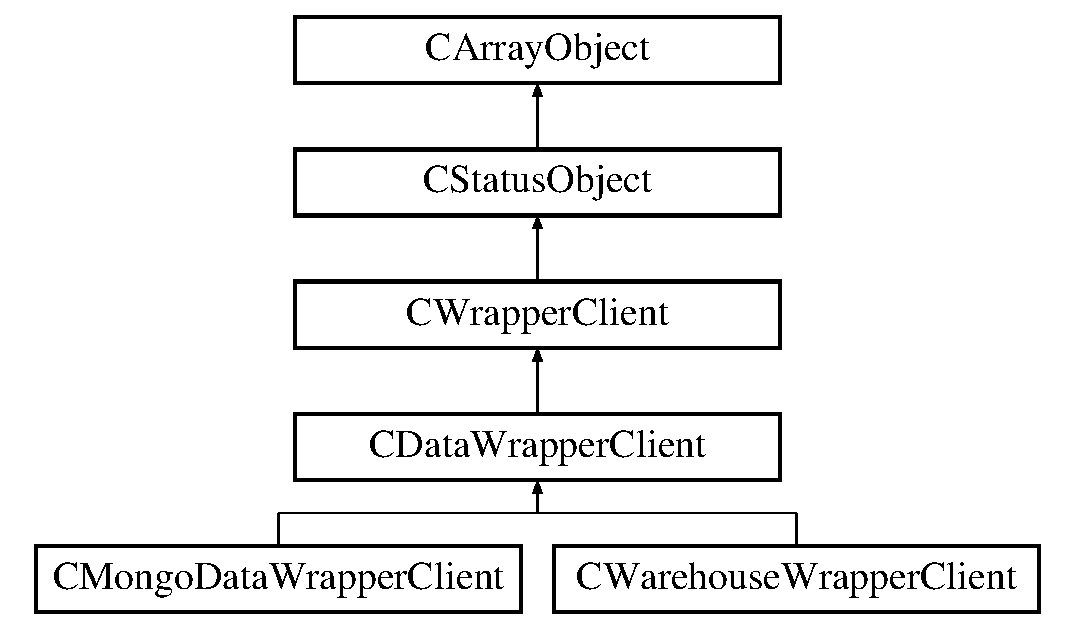
\includegraphics[height=5.000000cm]{class_c_data_wrapper_client}
\end{center}
\end{figure}
\subsection*{Public Member Functions}
\begin{DoxyCompactItemize}
\item 
\hyperlink{class_c_data_wrapper_client_ae7cad4809c20d8f2871cfe00da909d67}{Operation} (\$the\-Value=N\-U\-L\-L, \$get\-Old=F\-A\-L\-S\-E)
\item 
\hyperlink{class_c_data_wrapper_client_a4cdd14b07d74eeb834d2a6052902f176}{Database} (\$the\-Value=N\-U\-L\-L, \$get\-Old=F\-A\-L\-S\-E)
\item 
\hyperlink{class_c_data_wrapper_client_a6a696f83f580186da02093327a84fe4f}{Container} (\$the\-Value=N\-U\-L\-L, \$get\-Old=F\-A\-L\-S\-E)
\item 
\hyperlink{class_c_data_wrapper_client_ac07a1ae26e12e152090b397b4718c44c}{Start} (\$the\-Value=N\-U\-L\-L, \$get\-Old=F\-A\-L\-S\-E)
\item 
\hyperlink{class_c_data_wrapper_client_add9bd5c550e9ace4b69006b7ce65951a}{Limit} (\$the\-Value=N\-U\-L\-L, \$get\-Old=F\-A\-L\-S\-E)
\item 
\hyperlink{class_c_data_wrapper_client_a81a5e5f23f729bf167c03e6eee4593ed}{Query} (\$the\-Value=N\-U\-L\-L, \$get\-Old=F\-A\-L\-S\-E)
\item 
\hyperlink{class_c_data_wrapper_client_a61d1080dbd1fa5e8b805284a4bfa3581}{Fields} (\$the\-Value=N\-U\-L\-L, \$the\-Operation=N\-U\-L\-L, \$get\-Old=F\-A\-L\-S\-E)
\item 
\hyperlink{class_c_data_wrapper_client_abd1cbfe57fda4734cfd387fd0830272c}{Sort} (\$the\-Value=N\-U\-L\-L, \$get\-Old=F\-A\-L\-S\-E)
\item 
\hyperlink{class_c_data_wrapper_client_ab5a1dd1e3b56468f2748f9e1ecad92fc}{Object} (\$the\-Value=N\-U\-L\-L, \$get\-Old=F\-A\-L\-S\-E)
\item 
\hyperlink{class_c_data_wrapper_client_a5974e65e4ce07b93fc4b44ebffe5e606}{Options} (\$the\-Option=N\-U\-L\-L, \$the\-Value=N\-U\-L\-L, \$get\-Old=F\-A\-L\-S\-E)
\end{DoxyCompactItemize}
\subsection*{Additional Inherited Members}


\subsection{Member Function Documentation}
\hypertarget{class_c_data_wrapper_client_a6a696f83f580186da02093327a84fe4f}{\index{C\-Data\-Wrapper\-Client@{C\-Data\-Wrapper\-Client}!Container@{Container}}
\index{Container@{Container}!CDataWrapperClient@{C\-Data\-Wrapper\-Client}}
\subsubsection[{Container}]{\setlength{\rightskip}{0pt plus 5cm}C\-Data\-Wrapper\-Client\-::\-Container (
\begin{DoxyParamCaption}
\item[{}]{\$the\-Value = {\ttfamily NULL}, }
\item[{}]{\$get\-Old = {\ttfamily FALSE}}
\end{DoxyParamCaption}
)}}\label{class_c_data_wrapper_client_a6a696f83f580186da02093327a84fe4f}
Manage container.

This method can be used to manage the database \hyperlink{}{container}, it accepts a string which represents either the container name or the requested operation, depending on its value\-:


\begin{DoxyItemize}
\item {\itshape N\-U\-L\-L}\-: Return the current value. 
\item {\itshape F\-A\-L\-S\-E}\-: Delete the current value. 
\item {\itshape other}\-: Set the value with the provided parameter. 
\end{DoxyItemize}

The second parameter is a boolean which if {\itshape T\-R\-U\-E} will return the {\itshape old} value when replacing values; if {\itshape F\-A\-L\-S\-E}, it will return the currently set value.


\begin{DoxyParams}[1]{Parameters}
string & {\em \$the\-Value} & Value or operation. \\
\hline
boolean & {\em \$get\-Old} & T\-R\-U\-E get old value.\\
\hline
\end{DoxyParams}
public \begin{DoxyReturn}{Returns}
mixed
\end{DoxyReturn}
\hyperlink{class_c_attribute_a9d231a47718719fcd6c33f3d0ac91675}{C\-Attribute\-::\-Manage\-Offset()}

\begin{DoxySeeAlso}{See also}
k\-A\-P\-I\-\_\-\-C\-O\-N\-T\-A\-I\-N\-E\-R 
\end{DoxySeeAlso}
\hypertarget{class_c_data_wrapper_client_a4cdd14b07d74eeb834d2a6052902f176}{\index{C\-Data\-Wrapper\-Client@{C\-Data\-Wrapper\-Client}!Database@{Database}}
\index{Database@{Database}!CDataWrapperClient@{C\-Data\-Wrapper\-Client}}
\subsubsection[{Database}]{\setlength{\rightskip}{0pt plus 5cm}C\-Data\-Wrapper\-Client\-::\-Database (
\begin{DoxyParamCaption}
\item[{}]{\$the\-Value = {\ttfamily NULL}, }
\item[{}]{\$get\-Old = {\ttfamily FALSE}}
\end{DoxyParamCaption}
)}}\label{class_c_data_wrapper_client_a4cdd14b07d74eeb834d2a6052902f176}
Manage database.

This method can be used to manage the \hyperlink{}{database}, it accepts a string which represents either the database name or the requested operation, depending on its value\-:


\begin{DoxyItemize}
\item {\itshape N\-U\-L\-L}\-: Return the current value. 
\item {\itshape F\-A\-L\-S\-E}\-: Delete the current value. 
\item {\itshape other}\-: Set the value with the provided parameter. 
\end{DoxyItemize}

The second parameter is a boolean which if {\itshape T\-R\-U\-E} will return the {\itshape old} value when replacing values; if {\itshape F\-A\-L\-S\-E}, it will return the currently set value.


\begin{DoxyParams}[1]{Parameters}
string & {\em \$the\-Value} & Value or operation. \\
\hline
boolean & {\em \$get\-Old} & T\-R\-U\-E get old value.\\
\hline
\end{DoxyParams}
public \begin{DoxyReturn}{Returns}
mixed
\end{DoxyReturn}
\hyperlink{class_c_attribute_a9d231a47718719fcd6c33f3d0ac91675}{C\-Attribute\-::\-Manage\-Offset()}

\begin{DoxySeeAlso}{See also}
k\-A\-P\-I\-\_\-\-D\-A\-T\-A\-B\-A\-S\-E 
\end{DoxySeeAlso}
\hypertarget{class_c_data_wrapper_client_a61d1080dbd1fa5e8b805284a4bfa3581}{\index{C\-Data\-Wrapper\-Client@{C\-Data\-Wrapper\-Client}!Fields@{Fields}}
\index{Fields@{Fields}!CDataWrapperClient@{C\-Data\-Wrapper\-Client}}
\subsubsection[{Fields}]{\setlength{\rightskip}{0pt plus 5cm}C\-Data\-Wrapper\-Client\-::\-Fields (
\begin{DoxyParamCaption}
\item[{}]{\$the\-Value = {\ttfamily NULL}, }
\item[{}]{\$the\-Operation = {\ttfamily NULL}, }
\item[{}]{\$get\-Old = {\ttfamily FALSE}}
\end{DoxyParamCaption}
)}}\label{class_c_data_wrapper_client_a61d1080dbd1fa5e8b805284a4bfa3581}
Manage query fields.

This method can be used to manage the \hyperlink{}{fields} list, it accepts an array or Array\-Object which represents either the list of fields to be returned, or the requested operation, depending on its value\-:


\begin{DoxyItemize}
\item {\itshape N\-U\-L\-L}\-: Return the current value. 
\item {\itshape F\-A\-L\-S\-E}\-: Delete the current value. 
\item {\itshape other}\-: Set the value with the provided parameter. 
\end{DoxyItemize}

The second parameter is a boolean which if {\itshape T\-R\-U\-E} will return the {\itshape old} value when replacing values; if {\itshape F\-A\-L\-S\-E}, it will return the currently set value.

If the provided value is not an array or an Array\-Object, the method will raise an exception.


\begin{DoxyParams}[1]{Parameters}
mixed & {\em \$the\-Value} & Value or operation. \\
\hline
boolean & {\em \$get\-Old} & T\-R\-U\-E get old value.\\
\hline
\end{DoxyParams}
public \begin{DoxyReturn}{Returns}
mixed
\end{DoxyReturn}

\begin{DoxyExceptions}{Exceptions}
{\em \{@link} & \hyperlink{class_c_exception}{C\-Exception} \hyperlink{class_c_exception}{C\-Exception}\}\\
\hline
\end{DoxyExceptions}
\hyperlink{class_c_attribute_a9d231a47718719fcd6c33f3d0ac91675}{C\-Attribute\-::\-Manage\-Offset()}

\begin{DoxySeeAlso}{See also}
k\-A\-P\-I\-\_\-\-D\-A\-T\-A\-\_\-\-F\-I\-E\-L\-D 
\end{DoxySeeAlso}
\hypertarget{class_c_data_wrapper_client_add9bd5c550e9ace4b69006b7ce65951a}{\index{C\-Data\-Wrapper\-Client@{C\-Data\-Wrapper\-Client}!Limit@{Limit}}
\index{Limit@{Limit}!CDataWrapperClient@{C\-Data\-Wrapper\-Client}}
\subsubsection[{Limit}]{\setlength{\rightskip}{0pt plus 5cm}C\-Data\-Wrapper\-Client\-::\-Limit (
\begin{DoxyParamCaption}
\item[{}]{\$the\-Value = {\ttfamily NULL}, }
\item[{}]{\$get\-Old = {\ttfamily FALSE}}
\end{DoxyParamCaption}
)}}\label{class_c_data_wrapper_client_add9bd5c550e9ace4b69006b7ce65951a}
Manage page limit.

This method can be used to manage the page \hyperlink{}{limit}, it accepts a number which represents either the page limit or the requested operation, depending on its value\-:


\begin{DoxyItemize}
\item {\itshape N\-U\-L\-L}\-: Return the current value. 
\item {\itshape F\-A\-L\-S\-E}\-: Delete the current value. 
\item {\itshape other}\-: Set the value with the provided parameter. 
\end{DoxyItemize}

The second parameter is a boolean which if {\itshape T\-R\-U\-E} will return the {\itshape old} value when replacing values; if {\itshape F\-A\-L\-S\-E}, it will return the currently set value.


\begin{DoxyParams}[1]{Parameters}
integer & {\em \$the\-Value} & Value or operation. \\
\hline
boolean & {\em \$get\-Old} & T\-R\-U\-E get old value.\\
\hline
\end{DoxyParams}
public \begin{DoxyReturn}{Returns}
mixed
\end{DoxyReturn}
\hyperlink{class_c_attribute_a9d231a47718719fcd6c33f3d0ac91675}{C\-Attribute\-::\-Manage\-Offset()}

\begin{DoxySeeAlso}{See also}
k\-A\-P\-I\-\_\-\-P\-A\-G\-E\-\_\-\-L\-I\-M\-I\-T 
\end{DoxySeeAlso}
\hypertarget{class_c_data_wrapper_client_ab5a1dd1e3b56468f2748f9e1ecad92fc}{\index{C\-Data\-Wrapper\-Client@{C\-Data\-Wrapper\-Client}!Object@{Object}}
\index{Object@{Object}!CDataWrapperClient@{C\-Data\-Wrapper\-Client}}
\subsubsection[{Object}]{\setlength{\rightskip}{0pt plus 5cm}C\-Data\-Wrapper\-Client\-::\-Object (
\begin{DoxyParamCaption}
\item[{}]{\$the\-Value = {\ttfamily NULL}, }
\item[{}]{\$get\-Old = {\ttfamily FALSE}}
\end{DoxyParamCaption}
)}}\label{class_c_data_wrapper_client_ab5a1dd1e3b56468f2748f9e1ecad92fc}
Manage query object.

This method can be used to manage the \hyperlink{class_c_data_wrapper_client_a81a5e5f23f729bf167c03e6eee4593ed}{query} \hyperlink{}{object}, it accepts an array or Array\-Object which represents the object to be sent to the web-\/service, or the requested operation, depending on its value\-:


\begin{DoxyItemize}
\item {\itshape N\-U\-L\-L}\-: Return the current value. 
\item {\itshape F\-A\-L\-S\-E}\-: Delete the current value. 
\item {\itshape other}\-: Set the value with the provided parameter. 
\end{DoxyItemize}

The second parameter is a boolean which if {\itshape T\-R\-U\-E} will return the {\itshape old} value when replacing values; if {\itshape F\-A\-L\-S\-E}, it will return the currently set value.

If the provided value is not an array or an Array\-Object, the method will raise an exception.


\begin{DoxyParams}[1]{Parameters}
mixed & {\em \$the\-Value} & Value or operation. \\
\hline
boolean & {\em \$get\-Old} & T\-R\-U\-E get old value.\\
\hline
\end{DoxyParams}
public \begin{DoxyReturn}{Returns}
mixed
\end{DoxyReturn}

\begin{DoxyExceptions}{Exceptions}
{\em \{@link} & \hyperlink{class_c_exception}{C\-Exception} \hyperlink{class_c_exception}{C\-Exception}\}\\
\hline
\end{DoxyExceptions}
\hyperlink{class_c_attribute_a9d231a47718719fcd6c33f3d0ac91675}{C\-Attribute\-::\-Manage\-Offset()}

\begin{DoxySeeAlso}{See also}
k\-A\-P\-I\-\_\-\-D\-A\-T\-A\-\_\-\-O\-B\-J\-E\-C\-T 
\end{DoxySeeAlso}
\hypertarget{class_c_data_wrapper_client_ae7cad4809c20d8f2871cfe00da909d67}{\index{C\-Data\-Wrapper\-Client@{C\-Data\-Wrapper\-Client}!Operation@{Operation}}
\index{Operation@{Operation}!CDataWrapperClient@{C\-Data\-Wrapper\-Client}}
\subsubsection[{Operation}]{\setlength{\rightskip}{0pt plus 5cm}C\-Data\-Wrapper\-Client\-::\-Operation (
\begin{DoxyParamCaption}
\item[{}]{\$the\-Value = {\ttfamily NULL}, }
\item[{}]{\$get\-Old = {\ttfamily FALSE}}
\end{DoxyParamCaption}
)}}\label{class_c_data_wrapper_client_ae7cad4809c20d8f2871cfe00da909d67}
Manage operation.

We \hyperlink{class_c_wrapper_client_ae378229fd57b051ddf0e0a7abf599641}{overload} this method to add the following allowed operations\-:


\begin{DoxyItemize}
\item {\itshape \hyperlink{}{k\-A\-P\-I\-\_\-\-O\-P\-\_\-\-C\-O\-U\-N\-T}}\-: C\-O\-U\-N\-T web-\/service operation, used to return the total number of elements satisfying a query. 
\item {\itshape \hyperlink{}{k\-A\-P\-I\-\_\-\-O\-P\-\_\-\-M\-A\-T\-C\-H}}\-: This operation is equivalent to a read query, except that it will try to match one \hyperlink{}{query} clause at the time and will return a result on the first match. 
\item {\itshape \hyperlink{}{k\-A\-P\-I\-\_\-\-O\-P\-\_\-\-G\-E\-T}}\-: G\-E\-T web-\/service operation, used to retrieve objects from the data store. 
\item {\itshape \hyperlink{}{k\-A\-P\-I\-\_\-\-O\-P\-\_\-\-S\-E\-T}}\-: S\-E\-T web-\/service operation, used to insert or update objects in the data store. 
\item {\itshape \hyperlink{}{k\-A\-P\-I\-\_\-\-O\-P\-\_\-\-U\-P\-D\-A\-T\-E}}\-: U\-P\-D\-A\-T\-E web-\/service operation, used to update existing objects in the data store. 
\item {\itshape \hyperlink{}{k\-A\-P\-I\-\_\-\-O\-P\-\_\-\-I\-N\-S\-E\-R\-T}}\-: I\-N\-S\-E\-R\-T web-\/service operation, used to insert new objects in the data store. 
\item {\itshape \hyperlink{}{k\-A\-P\-I\-\_\-\-O\-P\-\_\-\-B\-A\-T\-C\-H\-\_\-\-I\-N\-S\-E\-R\-T}}\-: This service is equivalent to the \hyperlink{}{k\-A\-P\-I\-\_\-\-O\-P\-\_\-\-I\-N\-S\-E\-R\-T} command, except that in this case you provide a list ov objects to insert. 
\item {\itshape \hyperlink{}{k\-A\-P\-I\-\_\-\-O\-P\-\_\-\-M\-O\-D\-I\-F\-Y}}\-: M\-O\-D\-I\-F\-Y web-\/service operation, used to modify partial contents of objects in the data store. 
\item {\itshape \hyperlink{}{k\-A\-P\-I\-\_\-\-O\-P\-\_\-\-D\-E\-L}}\-: D\-E\-L\-E\-T\-E web-\/service operation, used to delete objects from the data store. 
\end{DoxyItemize}


\begin{DoxyParams}[1]{Parameters}
string & {\em \$the\-Value} & Value or operation. \\
\hline
boolean & {\em \$get\-Old} & T\-R\-U\-E get old value.\\
\hline
\end{DoxyParams}
public \begin{DoxyReturn}{Returns}
mixed
\end{DoxyReturn}

\begin{DoxyExceptions}{Exceptions}
{\em \{@link} & \hyperlink{class_c_exception}{C\-Exception} \hyperlink{class_c_exception}{C\-Exception}\}\\
\hline
\end{DoxyExceptions}
\hyperlink{class_c_attribute_a9d231a47718719fcd6c33f3d0ac91675}{C\-Attribute\-::\-Manage\-Offset()}

\begin{DoxySeeAlso}{See also}
k\-A\-P\-I\-\_\-\-O\-P\-E\-R\-A\-T\-I\-O\-N 

k\-A\-P\-I\-\_\-\-O\-P\-\_\-\-H\-E\-L\-P k\-A\-P\-I\-\_\-\-O\-P\-\_\-\-P\-I\-N\-G 
\end{DoxySeeAlso}


Reimplemented from \hyperlink{class_c_wrapper_client_ae378229fd57b051ddf0e0a7abf599641}{C\-Wrapper\-Client}.



Reimplemented in \hyperlink{class_c_mongo_data_wrapper_client_a730c4fe3a66ad8a5aa42e44f669632ac}{C\-Mongo\-Data\-Wrapper\-Client}, and \hyperlink{class_c_warehouse_wrapper_client_a099ef5aef1883aa5b394c7086a818496}{C\-Warehouse\-Wrapper\-Client}.

\hypertarget{class_c_data_wrapper_client_a5974e65e4ce07b93fc4b44ebffe5e606}{\index{C\-Data\-Wrapper\-Client@{C\-Data\-Wrapper\-Client}!Options@{Options}}
\index{Options@{Options}!CDataWrapperClient@{C\-Data\-Wrapper\-Client}}
\subsubsection[{Options}]{\setlength{\rightskip}{0pt plus 5cm}C\-Data\-Wrapper\-Client\-::\-Options (
\begin{DoxyParamCaption}
\item[{}]{\$the\-Option = {\ttfamily NULL}, }
\item[{}]{\$the\-Value = {\ttfamily NULL}, }
\item[{}]{\$get\-Old = {\ttfamily FALSE}}
\end{DoxyParamCaption}
)}}\label{class_c_data_wrapper_client_a5974e65e4ce07b93fc4b44ebffe5e606}
Manage options.

This method can be used to manage the \hyperlink{class_c_data_wrapper_client_a81a5e5f23f729bf167c03e6eee4593ed}{query} data \hyperlink{}{options}, with it you can add, retrieve and delete elements of the options list, to operate on the whole list you should use its \hyperlink{}{offset}.

The method accepts the following parameters\-:


\begin{DoxyItemize}
\item {\bfseries \$the\-Option}\-: This parameter represents the option, it can take the following values\-: 
\begin{DoxyItemize}
\item {\itshape \hyperlink{}{k\-A\-P\-I\-\_\-\-O\-P\-T\-\_\-\-S\-A\-F\-E}}\-: Can be a boolean or integer, defaults to F\-A\-L\-S\-E. If F\-A\-L\-S\-E, a database query will not wait for a response. If T\-R\-U\-E, the program will wait for the database response and throw an exception if the operation did not succeed. 
\item {\itshape \hyperlink{}{k\-A\-P\-I\-\_\-\-O\-P\-T\-\_\-\-F\-S\-Y\-N\-C}}\-: Boolean, defaults to F\-A\-L\-S\-E. Forces the update to be synced to disk before returning success. If T\-R\-U\-E, a \hyperlink{}{safe} update is implied and will override setting safe to F\-A\-L\-S\-E. 
\item {\itshape \hyperlink{}{k\-A\-P\-I\-\_\-\-O\-P\-T\-\_\-\-T\-I\-M\-E\-O\-U\-T}}\-: Integer, if \char`\"{}safe\char`\"{} is set, this sets how long (in milliseconds) for the client to wait for a database response. If the database does not respond within the timeout period, an exception will be thrown. 
\item {\itshape \hyperlink{}{k\-A\-P\-I\-\_\-\-O\-P\-T\-\_\-\-S\-I\-N\-G\-L\-E}}\-: Boolean, used in the \hyperlink{}{delete} or \hyperlink{}{update} operatiosn\-: if T\-R\-U\-E, only the first object will be affected; if not, all matching objects will be considered. 
\end{DoxyItemize}
\item {\bfseries \$the\-Value}\-: This parameter represents either the option value, or the operation to perform\-: 
\begin{DoxyItemize}
\item {\itshape N\-U\-L\-L}\-: This value indicates that we want to retrieve the value of the option provided in the previous parameter. 
\item {\itshape F\-A\-L\-S\-E}\-: This value indicates that we want to delete the option provided in the previous parameter. 
\item {\itshape other}\-: Any other value is interpreted as the value of the option selected by the first parameter. Note that, in general, missing options are equivalent to setting the option to {\itshape F\-A\-L\-S\-E}, when the value is a boolean, so turning off an option is the same as removing it. 
\end{DoxyItemize}
\item {\bfseries \$get\-Old}\-: Determines what the method will return\-: 
\begin{DoxyItemize}
\item {\itshape T\-R\-U\-E}\-: Return the element or list {\itshape before} it was eventually modified. 
\item {\itshape F\-A\-L\-S\-E}\-: Return the element or list {\itshape after} it was eventually modified. 
\end{DoxyItemize}
\end{DoxyItemize}


\begin{DoxyParams}[1]{Parameters}
mixed & {\em \$the\-Option} & Option selector. \\
\hline
mixed & {\em \$the\-Value} & Option value or operation. \\
\hline
boolean & {\em \$get\-Old} & T\-R\-U\-E get old value.\\
\hline
\end{DoxyParams}
public \begin{DoxyReturn}{Returns}
mixed
\end{DoxyReturn}

\begin{DoxyExceptions}{Exceptions}
{\em \{@link} & \hyperlink{class_c_exception}{C\-Exception} \hyperlink{class_c_exception}{C\-Exception}\}\\
\hline
\end{DoxyExceptions}
\begin{DoxySeeAlso}{See also}
k\-A\-P\-I\-\_\-\-D\-A\-T\-A\-\_\-\-O\-P\-T\-I\-O\-N\-S 
\end{DoxySeeAlso}
\hypertarget{class_c_data_wrapper_client_a81a5e5f23f729bf167c03e6eee4593ed}{\index{C\-Data\-Wrapper\-Client@{C\-Data\-Wrapper\-Client}!Query@{Query}}
\index{Query@{Query}!CDataWrapperClient@{C\-Data\-Wrapper\-Client}}
\subsubsection[{Query}]{\setlength{\rightskip}{0pt plus 5cm}C\-Data\-Wrapper\-Client\-::\-Query (
\begin{DoxyParamCaption}
\item[{}]{\$the\-Value = {\ttfamily NULL}, }
\item[{}]{\$get\-Old = {\ttfamily FALSE}}
\end{DoxyParamCaption}
)}}\label{class_c_data_wrapper_client_a81a5e5f23f729bf167c03e6eee4593ed}
Manage data query.

This method can be used to manage the data \hyperlink{}{query}, it accepts an array or Array\-Object which represents either the data query or the requested operation, depending on its value\-:


\begin{DoxyItemize}
\item {\itshape N\-U\-L\-L}\-: Return the current value. 
\item {\itshape F\-A\-L\-S\-E}\-: Delete the current value. 
\item {\itshape other}\-: Set the value with the provided parameter. 
\end{DoxyItemize}

The second parameter is a boolean which if {\itshape T\-R\-U\-E} will return the {\itshape old} value when replacing values; if {\itshape F\-A\-L\-S\-E}, it will return the currently set value.

If the provided value is not an array or an Array\-Object, the method will raise an exception.


\begin{DoxyParams}[1]{Parameters}
mixed & {\em \$the\-Value} & Value or operation. \\
\hline
boolean & {\em \$get\-Old} & T\-R\-U\-E get old value.\\
\hline
\end{DoxyParams}
public \begin{DoxyReturn}{Returns}
mixed
\end{DoxyReturn}

\begin{DoxyExceptions}{Exceptions}
{\em \{@link} & \hyperlink{class_c_exception}{C\-Exception} \hyperlink{class_c_exception}{C\-Exception}\}\\
\hline
\end{DoxyExceptions}
\hyperlink{class_c_attribute_a9d231a47718719fcd6c33f3d0ac91675}{C\-Attribute\-::\-Manage\-Offset()}

\begin{DoxySeeAlso}{See also}
k\-A\-P\-I\-\_\-\-D\-A\-T\-A\-\_\-\-Q\-U\-E\-R\-Y 
\end{DoxySeeAlso}
\hypertarget{class_c_data_wrapper_client_abd1cbfe57fda4734cfd387fd0830272c}{\index{C\-Data\-Wrapper\-Client@{C\-Data\-Wrapper\-Client}!Sort@{Sort}}
\index{Sort@{Sort}!CDataWrapperClient@{C\-Data\-Wrapper\-Client}}
\subsubsection[{Sort}]{\setlength{\rightskip}{0pt plus 5cm}C\-Data\-Wrapper\-Client\-::\-Sort (
\begin{DoxyParamCaption}
\item[{}]{\$the\-Value = {\ttfamily NULL}, }
\item[{}]{\$get\-Old = {\ttfamily FALSE}}
\end{DoxyParamCaption}
)}}\label{class_c_data_wrapper_client_abd1cbfe57fda4734cfd387fd0830272c}
Manage sort fields.

This method can be used to manage the \hyperlink{class_c_data_wrapper_client_a81a5e5f23f729bf167c03e6eee4593ed}{query} \hyperlink{}{sort} fields, it accepts an array or Array\-Object which represents either the \hyperlink{class_c_data_wrapper_client_a81a5e5f23f729bf167c03e6eee4593ed}{query} list of sort fields, or the requested operation, depending on its value\-:


\begin{DoxyItemize}
\item {\itshape N\-U\-L\-L}\-: Return the current value. 
\item {\itshape F\-A\-L\-S\-E}\-: Delete the current value. 
\item {\itshape other}\-: Set the value with the provided parameter. 
\end{DoxyItemize}

The second parameter is a boolean which if {\itshape T\-R\-U\-E} will return the {\itshape old} value when replacing values; if {\itshape F\-A\-L\-S\-E}, it will return the currently set value.

If the provided value is not an array or an Array\-Object, the method will raise an exception.


\begin{DoxyParams}[1]{Parameters}
mixed & {\em \$the\-Value} & Value or operation. \\
\hline
boolean & {\em \$get\-Old} & T\-R\-U\-E get old value.\\
\hline
\end{DoxyParams}
public \begin{DoxyReturn}{Returns}
mixed
\end{DoxyReturn}

\begin{DoxyExceptions}{Exceptions}
{\em \{@link} & \hyperlink{class_c_exception}{C\-Exception} \hyperlink{class_c_exception}{C\-Exception}\}\\
\hline
\end{DoxyExceptions}
\hyperlink{class_c_attribute_a9d231a47718719fcd6c33f3d0ac91675}{C\-Attribute\-::\-Manage\-Offset()}

\begin{DoxySeeAlso}{See also}
k\-A\-P\-I\-\_\-\-D\-A\-T\-A\-\_\-\-S\-O\-R\-T 
\end{DoxySeeAlso}
\hypertarget{class_c_data_wrapper_client_ac07a1ae26e12e152090b397b4718c44c}{\index{C\-Data\-Wrapper\-Client@{C\-Data\-Wrapper\-Client}!Start@{Start}}
\index{Start@{Start}!CDataWrapperClient@{C\-Data\-Wrapper\-Client}}
\subsubsection[{Start}]{\setlength{\rightskip}{0pt plus 5cm}C\-Data\-Wrapper\-Client\-::\-Start (
\begin{DoxyParamCaption}
\item[{}]{\$the\-Value = {\ttfamily NULL}, }
\item[{}]{\$get\-Old = {\ttfamily FALSE}}
\end{DoxyParamCaption}
)}}\label{class_c_data_wrapper_client_ac07a1ae26e12e152090b397b4718c44c}
Manage page start.

This method can be used to manage the page \hyperlink{}{start}, it accepts a number which represents either the page start or the requested operation, depending on its value\-:


\begin{DoxyItemize}
\item {\itshape N\-U\-L\-L}\-: Return the current value. 
\item {\itshape F\-A\-L\-S\-E}\-: Delete the current value. 
\item {\itshape other}\-: Set the value with the provided parameter. 
\end{DoxyItemize}

The second parameter is a boolean which if {\itshape T\-R\-U\-E} will return the {\itshape old} value when replacing values; if {\itshape F\-A\-L\-S\-E}, it will return the currently set value.


\begin{DoxyParams}[1]{Parameters}
integer & {\em \$the\-Value} & Value or operation. \\
\hline
boolean & {\em \$get\-Old} & T\-R\-U\-E get old value.\\
\hline
\end{DoxyParams}
public \begin{DoxyReturn}{Returns}
mixed
\end{DoxyReturn}
\hyperlink{class_c_attribute_a9d231a47718719fcd6c33f3d0ac91675}{C\-Attribute\-::\-Manage\-Offset()}

\begin{DoxySeeAlso}{See also}
k\-A\-P\-I\-\_\-\-P\-A\-G\-E\-\_\-\-S\-T\-A\-R\-T 
\end{DoxySeeAlso}


The documentation for this class was generated from the following file\-:\begin{DoxyCompactItemize}
\item 
/\-Library/\-Web\-Server/\-Library/wrapper/classes/C\-Data\-Wrapper\-Client.\-php\end{DoxyCompactItemize}

\hypertarget{class_c_entity}{\section{C\-Entity Class Reference}
\label{class_c_entity}\index{C\-Entity@{C\-Entity}}
}
Inheritance diagram for C\-Entity\-:\begin{figure}[H]
\begin{center}
\leavevmode
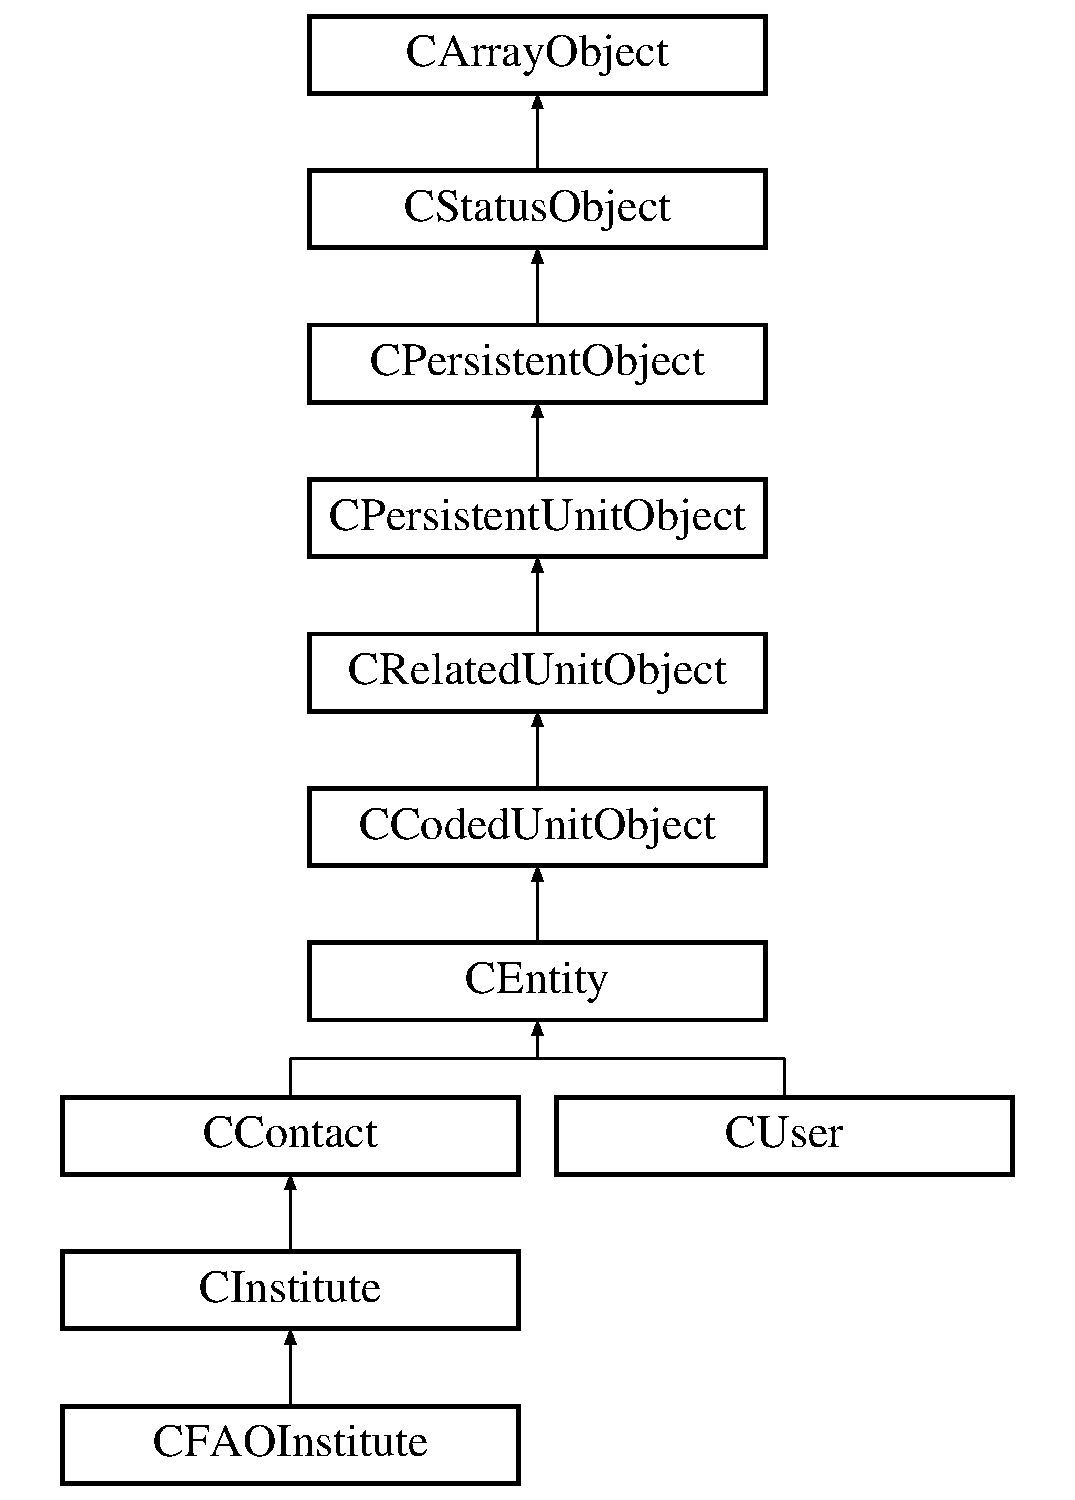
\includegraphics[height=6.000000cm]{class_c_entity}
\end{center}
\end{figure}
\subsection*{Public Member Functions}
\begin{DoxyCompactItemize}
\item 
\hyperlink{class_c_entity_ac087e5b3d14357f452ab531db5f6a7e9}{\-\_\-\-\_\-construct} (\$the\-Container=N\-U\-L\-L, \$the\-Identifier=N\-U\-L\-L)
\item 
\hyperlink{class_c_entity_a78127acb8de5ae1e7238566396dd1c17}{Type} (\$the\-Value=N\-U\-L\-L, \$the\-Operation=N\-U\-L\-L, \$get\-Old=F\-A\-L\-S\-E)
\item 
\hyperlink{class_c_entity_a2b3cf77715881c3d8b3a6d4d80042e7c}{Code} (\$the\-Value=N\-U\-L\-L, \$get\-Old=F\-A\-L\-S\-E)
\item 
\hyperlink{class_c_entity_ace5878c009baf09d85c8ca115c48dbb0}{Name} (\$the\-Value=N\-U\-L\-L, \$get\-Old=F\-A\-L\-S\-E)
\item 
\hyperlink{class_c_entity_a44b389a90107f4c8aadcc4eb08e1ad9b}{Mail} (\$the\-Type=N\-U\-L\-L, \$the\-Value=N\-U\-L\-L, \$get\-Old=F\-A\-L\-S\-E)
\item 
\hyperlink{class_c_entity_acf65b6fb2f4195f6c649b4ca506c7899}{Email} (\$the\-Value=N\-U\-L\-L, \$get\-Old=F\-A\-L\-S\-E)
\item 
\hyperlink{class_c_entity_ac69e40a0ee4489abfcc7241d98b07532}{Phone} (\$the\-Value=N\-U\-L\-L, \$get\-Old=F\-A\-L\-S\-E)
\item 
\hyperlink{class_c_entity_ac8fc97b7adfc8ce547db5f93a9b913a8}{Parent} (\$the\-Value, \$the\-Operation=N\-U\-L\-L, \$get\-Old=F\-A\-L\-S\-E)
\item 
\hyperlink{class_c_entity_a193cf3d19057021bb6e779644730eac8}{offset\-Set} (\$the\-Offset, \$the\-Value)
\item 
\hyperlink{class_c_entity_a887a87fc716e36a0d4c1477dbaf5bb67}{offset\-Unset} (\$the\-Offset)
\end{DoxyCompactItemize}
\subsection*{Static Public Member Functions}
\begin{DoxyCompactItemize}
\item 
static \hyperlink{class_c_entity_a260a4c309aff31a42d0e23b372f9b209}{Default\-Container} ()
\end{DoxyCompactItemize}
\subsection*{Protected Member Functions}
\begin{DoxyCompactItemize}
\item 
\hyperlink{class_c_entity_a991f328223b1b00b37e9028b16f7a7c8}{\-\_\-\-Prepare\-Store} (\&\$the\-Container, \&\$the\-Identifier)
\item 
\hyperlink{class_c_entity_ac518d3885e2c6f30051b8c5ec59e50a3}{\-\_\-id} ()
\end{DoxyCompactItemize}


\subsection{Constructor \& Destructor Documentation}
\hypertarget{class_c_entity_ac087e5b3d14357f452ab531db5f6a7e9}{\index{C\-Entity@{C\-Entity}!\-\_\-\-\_\-construct@{\-\_\-\-\_\-construct}}
\index{\-\_\-\-\_\-construct@{\-\_\-\-\_\-construct}!CEntity@{C\-Entity}}
\subsubsection[{\-\_\-\-\_\-construct}]{\setlength{\rightskip}{0pt plus 5cm}{\bf C\-Entity\-::\-\_\-\-\_\-construct} (
\begin{DoxyParamCaption}
\item[{\$}]{the\-Container = {\ttfamily NULL}, }
\item[{\$}]{the\-Identifier = {\ttfamily NULL}}
\end{DoxyParamCaption}
)}}\label{class_c_entity_ac087e5b3d14357f452ab531db5f6a7e9}
Instantiate class.

We \hyperlink{class_c_persistent_object_a10d0ce97598da33eaf305eb43e418255}{overload} the constructor to initialise the \hyperlink{class_c_status_object_a8429102e4f52f7558649b64f4e673a69}{inited} \hyperlink{}{flag} if the \hyperlink{class_c_entity_a2b3cf77715881c3d8b3a6d4d80042e7c}{code} and \hyperlink{class_c_entity_ace5878c009baf09d85c8ca115c48dbb0}{name} elements are set.


\begin{DoxyParams}[1]{Parameters}
mixed & {\em \$the\-Container} & Persistent container. \\
\hline
mixed & {\em \$the\-Identifier} & Object identifier.\\
\hline
\end{DoxyParams}
public 

Reimplemented from \hyperlink{class_c_persistent_object_a10d0ce97598da33eaf305eb43e418255}{C\-Persistent\-Object}.



Reimplemented in \hyperlink{class_c_user_a728ac6fd50a9f9e18dfe2fa547d5c798}{C\-User}.



\subsection{Member Function Documentation}
\hypertarget{class_c_entity_ac518d3885e2c6f30051b8c5ec59e50a3}{\index{C\-Entity@{C\-Entity}!\-\_\-id@{\-\_\-id}}
\index{\-\_\-id@{\-\_\-id}!CEntity@{C\-Entity}}
\subsubsection[{\-\_\-id}]{\setlength{\rightskip}{0pt plus 5cm}{\bf C\-Entity\-::\-\_\-id} (
\begin{DoxyParamCaption}
{}
\end{DoxyParamCaption}
)\hspace{0.3cm}{\ttfamily  \mbox{[}protected\mbox{]}}}}\label{class_c_entity_ac518d3885e2c6f30051b8c5ec59e50a3}
Return the object's unique identifier.

We overload this method to return the object's \hyperlink{}{identifier}, if it is set, or the object's \hyperlink{class_c_entity_a2b3cf77715881c3d8b3a6d4d80042e7c}{code}.

If none of the above are set, we call the parent method.

protected \begin{DoxyReturn}{Returns}
string 
\end{DoxyReturn}


Reimplemented from \hyperlink{class_c_persistent_unit_object_ad1ca0920cf0df3c24351402f9afbf34b}{C\-Persistent\-Unit\-Object}.

\hypertarget{class_c_entity_a991f328223b1b00b37e9028b16f7a7c8}{\index{C\-Entity@{C\-Entity}!\-\_\-\-Prepare\-Store@{\-\_\-\-Prepare\-Store}}
\index{\-\_\-\-Prepare\-Store@{\-\_\-\-Prepare\-Store}!CEntity@{C\-Entity}}
\subsubsection[{\-\_\-\-Prepare\-Store}]{\setlength{\rightskip}{0pt plus 5cm}{\bf C\-Entity\-::\-\_\-\-Prepare\-Store} (
\begin{DoxyParamCaption}
\item[{\&\$}]{the\-Container, }
\item[{\&\$}]{the\-Identifier}
\end{DoxyParamCaption}
)\hspace{0.3cm}{\ttfamily  \mbox{[}protected\mbox{]}}}}\label{class_c_entity_a991f328223b1b00b37e9028b16f7a7c8}
Normalise before a store.

We overload this method to check if the object in \hyperlink{class_c_status_object_a8429102e4f52f7558649b64f4e673a69}{initialised}, if this is not the case we raise an exception.


\begin{DoxyParams}[1]{Parameters}
reference & {\em \&\$the\-Container} & Object container. \\
\hline
reference & {\em \&\$the\-Identifier} & Object identifier.\\
\hline
\end{DoxyParams}
protected


\begin{DoxyExceptions}{Exceptions}
{\em \hyperlink{class_c_exception}{C\-Exception}} & \\
\hline
\end{DoxyExceptions}
\begin{DoxySeeAlso}{See also}
k\-E\-R\-R\-O\-R\-\_\-\-O\-P\-T\-I\-O\-N\-\_\-\-M\-I\-S\-S\-I\-N\-G 
\end{DoxySeeAlso}


Reimplemented from \hyperlink{class_c_persistent_unit_object_a42b46ccb307aa8038e5ed78819a23aa6}{C\-Persistent\-Unit\-Object}.



Reimplemented in \hyperlink{class_c_user_a031f5d13fe837cf445006ee21023bf3e}{C\-User}.

\hypertarget{class_c_entity_a2b3cf77715881c3d8b3a6d4d80042e7c}{\index{C\-Entity@{C\-Entity}!Code@{Code}}
\index{Code@{Code}!CEntity@{C\-Entity}}
\subsubsection[{Code}]{\setlength{\rightskip}{0pt plus 5cm}{\bf C\-Entity\-::\-Code} (
\begin{DoxyParamCaption}
\item[{\$}]{the\-Value = {\ttfamily NULL}, }
\item[{\$}]{get\-Old = {\ttfamily FALSE}}
\end{DoxyParamCaption}
)}}\label{class_c_entity_a2b3cf77715881c3d8b3a6d4d80042e7c}
Manage entity code.

This method can be used to manage the entity \hyperlink{}{code}, it uses the standard accessor \hyperlink{class_c_array_object_a931cb8b30569b811a18adc0161eb3603}{method} to manage the \hyperlink{}{offset}\-:

For a more in-\/depth reference of this method, please consult the \hyperlink{class_c_array_object_a931cb8b30569b811a18adc0161eb3603}{\-\_\-\-Manage\-Offset} method, in which the first parameter will be the constant \hyperlink{}{k\-T\-A\-G\-\_\-\-C\-O\-D\-E}.


\begin{DoxyParams}[1]{Parameters}
mixed & {\em \$the\-Value} & Value. \\
\hline
boolean & {\em \$get\-Old} & T\-R\-U\-E get old value.\\
\hline
\end{DoxyParams}
public \begin{DoxyReturn}{Returns}
string 
\end{DoxyReturn}
\hypertarget{class_c_entity_a260a4c309aff31a42d0e23b372f9b209}{\index{C\-Entity@{C\-Entity}!Default\-Container@{Default\-Container}}
\index{Default\-Container@{Default\-Container}!CEntity@{C\-Entity}}
\subsubsection[{Default\-Container}]{\setlength{\rightskip}{0pt plus 5cm}static {\bf C\-Entity\-::\-Default\-Container} (
\begin{DoxyParamCaption}
{}
\end{DoxyParamCaption}
)\hspace{0.3cm}{\ttfamily  \mbox{[}static\mbox{]}}}}\label{class_c_entity_a260a4c309aff31a42d0e23b372f9b209}
Return the default container.

This method can be used to retrieve the default container name.

\begin{DoxyReturn}{Returns}
string 
\end{DoxyReturn}
\hypertarget{class_c_entity_acf65b6fb2f4195f6c649b4ca506c7899}{\index{C\-Entity@{C\-Entity}!Email@{Email}}
\index{Email@{Email}!CEntity@{C\-Entity}}
\subsubsection[{Email}]{\setlength{\rightskip}{0pt plus 5cm}{\bf C\-Entity\-::\-Email} (
\begin{DoxyParamCaption}
\item[{\$}]{the\-Value = {\ttfamily NULL}, }
\item[{\$}]{get\-Old = {\ttfamily FALSE}}
\end{DoxyParamCaption}
)}}\label{class_c_entity_acf65b6fb2f4195f6c649b4ca506c7899}
Manage entity e-\/mail.

This method can be used to manage the entity \hyperlink{}{e-\/mail}, it uses the standard accessor \hyperlink{class_c_array_object_a931cb8b30569b811a18adc0161eb3603}{method} to manage the \hyperlink{}{offset}\-:

For a more in-\/depth reference of this method, please consult the \hyperlink{class_c_array_object_a931cb8b30569b811a18adc0161eb3603}{\-\_\-\-Manage\-Offset} method, in which the first parameter will be the constant \hyperlink{}{k\-O\-F\-F\-S\-E\-T\-\_\-\-E\-M\-A\-I\-L}.


\begin{DoxyParams}[1]{Parameters}
mixed & {\em \$the\-Value} & Value. \\
\hline
boolean & {\em \$get\-Old} & T\-R\-U\-E get old value.\\
\hline
\end{DoxyParams}
public \begin{DoxyReturn}{Returns}
string 
\end{DoxyReturn}
\hypertarget{class_c_entity_a44b389a90107f4c8aadcc4eb08e1ad9b}{\index{C\-Entity@{C\-Entity}!Mail@{Mail}}
\index{Mail@{Mail}!CEntity@{C\-Entity}}
\subsubsection[{Mail}]{\setlength{\rightskip}{0pt plus 5cm}{\bf C\-Entity\-::\-Mail} (
\begin{DoxyParamCaption}
\item[{\$}]{the\-Type = {\ttfamily NULL}, }
\item[{\$}]{the\-Value = {\ttfamily NULL}, }
\item[{\$}]{get\-Old = {\ttfamily FALSE}}
\end{DoxyParamCaption}
)}}\label{class_c_entity_a44b389a90107f4c8aadcc4eb08e1ad9b}
Manage entity mailing addresses.

This method can be used to manage the entity mailing \hyperlink{}{addresses}, it uses the standard accessor \hyperlink{class_c_array_object_af714f81bb75f725c6868fb286c59b160}{method} to manage the list of addresses.

This list is an array of structures where the \hyperlink{}{k\-T\-A\-G\-\_\-\-T\-Y\-P\-E} element indicates the type of the address, for instance {\itshape home\/} or office, and the \hyperlink{}{k\-T\-A\-G\-\_\-\-D\-A\-T\-A} element represents the actual address, be it a string or itself a structure holding the address elements. If the \hyperlink{}{k\-T\-A\-G\-\_\-\-T\-Y\-P\-E} element is missing, we assume it to be the default address.

For a more in-\/depth reference of this method, please consult the \hyperlink{class_c_array_object_a056b7a3218ffb9a2eb992c029124a669}{\-\_\-\-Manage\-Typed\-Array\-Offset} method, in which the first parameter will be the constant \hyperlink{}{k\-O\-F\-F\-S\-E\-T\-\_\-\-M\-A\-I\-L}.

Note that this method will $<$i$<$N\-O\-T work on an object that was \hyperlink{class_c_mongo_data_wrapper_a0d37f7b47e1a1ac48846f6d10d08d846}{serialised}.


\begin{DoxyParams}[1]{Parameters}
mixed & {\em \$the\-Type} & Item type. \\
\hline
mixed & {\em \$the\-Value} & Item value. \\
\hline
boolean & {\em \$get\-Old} & T\-R\-U\-E get old value.\\
\hline
\end{DoxyParams}
public \begin{DoxyReturn}{Returns}
string 
\end{DoxyReturn}
\hypertarget{class_c_entity_ace5878c009baf09d85c8ca115c48dbb0}{\index{C\-Entity@{C\-Entity}!Name@{Name}}
\index{Name@{Name}!CEntity@{C\-Entity}}
\subsubsection[{Name}]{\setlength{\rightskip}{0pt plus 5cm}{\bf C\-Entity\-::\-Name} (
\begin{DoxyParamCaption}
\item[{\$}]{the\-Value = {\ttfamily NULL}, }
\item[{\$}]{get\-Old = {\ttfamily FALSE}}
\end{DoxyParamCaption}
)}}\label{class_c_entity_ace5878c009baf09d85c8ca115c48dbb0}
Manage entity name.

This method can be used to manage the entity \hyperlink{}{name}, it uses the standard accessor \hyperlink{class_c_array_object_a931cb8b30569b811a18adc0161eb3603}{method} to manage the \hyperlink{}{offset}\-:

For a more in-\/depth reference of this method, please consult the \hyperlink{class_c_array_object_a931cb8b30569b811a18adc0161eb3603}{\-\_\-\-Manage\-Offset} method, in which the first parameter will be the constant \hyperlink{}{k\-T\-A\-G\-\_\-\-N\-A\-M\-E}.


\begin{DoxyParams}[1]{Parameters}
mixed & {\em \$the\-Value} & Value. \\
\hline
boolean & {\em \$get\-Old} & T\-R\-U\-E get old value.\\
\hline
\end{DoxyParams}
public \begin{DoxyReturn}{Returns}
string 
\end{DoxyReturn}
\hypertarget{class_c_entity_a193cf3d19057021bb6e779644730eac8}{\index{C\-Entity@{C\-Entity}!offset\-Set@{offset\-Set}}
\index{offset\-Set@{offset\-Set}!CEntity@{C\-Entity}}
\subsubsection[{offset\-Set}]{\setlength{\rightskip}{0pt plus 5cm}{\bf C\-Entity\-::offset\-Set} (
\begin{DoxyParamCaption}
\item[{\$}]{the\-Offset, }
\item[{\$}]{the\-Value}
\end{DoxyParamCaption}
)}}\label{class_c_entity_a193cf3d19057021bb6e779644730eac8}
Set a value for a given offset.

We overload this method to manage the \hyperlink{}{Inited() inited} \hyperlink{}{status}\-: this is set if \hyperlink{}{code} and \hyperlink{}{name} properties are set.


\begin{DoxyParams}[1]{Parameters}
string & {\em \$the\-Offset} & Offset. \\
\hline
string | N\-U\-L\-L & {\em \$the\-Value} & Value to set at offset.\\
\hline
\end{DoxyParams}
public 

Reimplemented from \hyperlink{class_c_status_object_a140ef140d4fa1c4a6180e843bd5ec969}{C\-Status\-Object}.



Reimplemented in \hyperlink{class_c_user_aace3446b9cacfe28cc1937c608fcc999}{C\-User}.

\hypertarget{class_c_entity_a887a87fc716e36a0d4c1477dbaf5bb67}{\index{C\-Entity@{C\-Entity}!offset\-Unset@{offset\-Unset}}
\index{offset\-Unset@{offset\-Unset}!CEntity@{C\-Entity}}
\subsubsection[{offset\-Unset}]{\setlength{\rightskip}{0pt plus 5cm}{\bf C\-Entity\-::offset\-Unset} (
\begin{DoxyParamCaption}
\item[{\$}]{the\-Offset}
\end{DoxyParamCaption}
)}}\label{class_c_entity_a887a87fc716e36a0d4c1477dbaf5bb67}
Reset a value for a given offset.

We overload this method to manage the \hyperlink{}{Inited() inited} \hyperlink{}{status}\-: this is set if \hyperlink{}{code} and \hyperlink{}{name} properties are set.


\begin{DoxyParams}[1]{Parameters}
string & {\em \$the\-Offset} & Offset.\\
\hline
\end{DoxyParams}
public 

Reimplemented from \hyperlink{class_c_status_object_ae733db1bbfffcbe894ea405765ab4150}{C\-Status\-Object}.



Reimplemented in \hyperlink{class_c_user_aed8557e18a89d868cedf5a48328b33b2}{C\-User}.

\hypertarget{class_c_entity_ac8fc97b7adfc8ce547db5f93a9b913a8}{\index{C\-Entity@{C\-Entity}!Parent@{Parent}}
\index{Parent@{Parent}!CEntity@{C\-Entity}}
\subsubsection[{Parent}]{\setlength{\rightskip}{0pt plus 5cm}{\bf C\-Entity\-::\-Parent} (
\begin{DoxyParamCaption}
\item[{\$}]{the\-Value, }
\item[{\$}]{the\-Operation = {\ttfamily NULL}, }
\item[{\$}]{get\-Old = {\ttfamily FALSE}}
\end{DoxyParamCaption}
)}}\label{class_c_entity_ac8fc97b7adfc8ce547db5f93a9b913a8}
Manage entity parents.

This method can be used to manage the entity \hyperlink{}{parents}, you can add/replace, retrieve and delete parent elements depending on the value of the parameters.

The property is represented by an array of instances derived from this class, or strings representing entity \hyperlink{}{identifiers}. In the first case, prior to \hyperlink{class_c_persistent_object_ad076a9a2baf73bba0784deb135a3b7b7}{saving} the current object, array elements in the form of \hyperlink{class_c_entity}{C\-Entity} instances will also be \hyperlink{class_c_persistent_object_ad076a9a2baf73bba0784deb135a3b7b7}{saved} and replaced by their \hyperlink{}{identifiers}.

This method accepts the following parameters\-:


\begin{DoxyItemize}
\item {\bfseries \$the\-Index}\-: This parameter represents the element index. 
\item {\bfseries \$the\-Operation}\-: The operation to perform\-: 
\begin{DoxyItemize}
\item {\itshape N\-U\-L\-L\/}\-: Retrieve the element, the methoid will return the matching element or {\itshape N\-U\-L\-L\/} if not found. 
\item {\itshape F\-A\-L\-S\-E\/}\-: Delete the element, depending on the value of the next parameter, the method will either return the deleted element or {\itshape N\-U\-L\-L\/}. 
\item {\itshape other\/}\-: Any other value means that we want to add/replace the element, in this case the method will return the added element's index. 
\end{DoxyItemize}
\item {\bfseries \$the\-Data}\-: This parameter represents the element data. 
\end{DoxyItemize}

Note that this method will $<$i$<$N\-O\-T work on an object that was \hyperlink{class_c_mongo_data_wrapper_a0d37f7b47e1a1ac48846f6d10d08d846}{serialised}.


\begin{DoxyParams}[1]{Parameters}
mixed & {\em \$the\-Value} & Index or value. \\
\hline
mixed & {\em \$the\-Operation} & Operation. \\
\hline
boolean & {\em \$get\-Old} & T\-R\-U\-E get old value.\\
\hline
\end{DoxyParams}
public \begin{DoxyReturn}{Returns}
string 
\end{DoxyReturn}
\hypertarget{class_c_entity_ac69e40a0ee4489abfcc7241d98b07532}{\index{C\-Entity@{C\-Entity}!Phone@{Phone}}
\index{Phone@{Phone}!CEntity@{C\-Entity}}
\subsubsection[{Phone}]{\setlength{\rightskip}{0pt plus 5cm}{\bf C\-Entity\-::\-Phone} (
\begin{DoxyParamCaption}
\item[{\$}]{the\-Value = {\ttfamily NULL}, }
\item[{\$}]{get\-Old = {\ttfamily FALSE}}
\end{DoxyParamCaption}
)}}\label{class_c_entity_ac69e40a0ee4489abfcc7241d98b07532}
Manage entity phone.

This method can be used to manage the entity \hyperlink{}{telephone} number, it uses the standard accessor \hyperlink{class_c_array_object_a931cb8b30569b811a18adc0161eb3603}{method} to manage the \hyperlink{}{offset}\-:

For a more in-\/depth reference of this method, please consult the \hyperlink{class_c_array_object_a931cb8b30569b811a18adc0161eb3603}{\-\_\-\-Manage\-Offset} method, in which the first parameter will be the constant \hyperlink{}{k\-O\-F\-F\-S\-E\-T\-\_\-\-P\-H\-O\-N\-E}.


\begin{DoxyParams}[1]{Parameters}
mixed & {\em \$the\-Value} & Value. \\
\hline
boolean & {\em \$get\-Old} & T\-R\-U\-E get old value.\\
\hline
\end{DoxyParams}
public \begin{DoxyReturn}{Returns}
string 
\end{DoxyReturn}
\hypertarget{class_c_entity_a78127acb8de5ae1e7238566396dd1c17}{\index{C\-Entity@{C\-Entity}!Type@{Type}}
\index{Type@{Type}!CEntity@{C\-Entity}}
\subsubsection[{Type}]{\setlength{\rightskip}{0pt plus 5cm}{\bf C\-Entity\-::\-Type} (
\begin{DoxyParamCaption}
\item[{\$}]{the\-Value = {\ttfamily NULL}, }
\item[{\$}]{the\-Operation = {\ttfamily NULL}, }
\item[{\$}]{get\-Old = {\ttfamily FALSE}}
\end{DoxyParamCaption}
)}}\label{class_c_entity_a78127acb8de5ae1e7238566396dd1c17}
Manage entity types.

This method can be used to manage the entity \hyperlink{}{types}, it uses the standard accessor \hyperlink{class_c_array_object_a056b7a3218ffb9a2eb992c029124a669}{method} to manage the list of parent entities.

In general, elements of this list should be a token that indicates a specific function of the entity, this could be, for instance', {\itshape user\/} to indicate an entity that is also a user of the system.

For a more in-\/depth reference of this method, please consult the \hyperlink{class_c_array_object_a056b7a3218ffb9a2eb992c029124a669}{\-\_\-\-Manage\-Array\-Offset} method, in which the first parameter will be the constant \hyperlink{}{k\-T\-A\-G\-\_\-\-T\-Y\-P\-E}.

Note that this method will $<$i$<$N\-O\-T work on an object that was \hyperlink{class_c_mongo_data_wrapper_a0d37f7b47e1a1ac48846f6d10d08d846}{serialised}.


\begin{DoxyParams}[1]{Parameters}
mixed & {\em \$the\-Value} & Value or index. \\
\hline
mixed & {\em \$the\-Operation} & Operation. \\
\hline
boolean & {\em \$get\-Old} & T\-R\-U\-E get old value.\\
\hline
\end{DoxyParams}
public \begin{DoxyReturn}{Returns}
string 
\end{DoxyReturn}


The documentation for this class was generated from the following file\-:\begin{DoxyCompactItemize}
\item 
/\-Library/\-Web\-Server/\-Library/wrapper/classes/C\-Entity.\-php\end{DoxyCompactItemize}

\hypertarget{class_c_exception}{\section{C\-Exception Class Reference}
\label{class_c_exception}\index{C\-Exception@{C\-Exception}}
}
\subsection*{Public Member Functions}
\begin{DoxyCompactItemize}
\item 
\hyperlink{class_c_exception_aea9f2ae76b6058652dfb672ce1a78507}{\-\_\-\-\_\-construct} (\$the\-Message=N\-U\-L\-L, \$the\-Code=N\-U\-L\-L, \$the\-Severity=N\-U\-L\-L, \$the\-References=N\-U\-L\-L, \$the\-Previous=N\-U\-L\-L)
\item 
\hyperlink{class_c_exception_a06b1b207799f8a8ca27bc12d1be82b07}{\-\_\-\-\_\-to\-String} ()
\item 
\hyperlink{class_c_exception_a2bef90da8a35e80dda8072d4f748ec20}{Severity} (\$the\-Value=N\-U\-L\-L)
\item 
\hyperlink{class_c_exception_abcbd46a262790fcbe3493e30a6418821}{Reference} (\$the\-Index=N\-U\-L\-L, \$the\-Value=N\-U\-L\-L)
\end{DoxyCompactItemize}
\subsection*{Static Public Member Functions}
\begin{DoxyCompactItemize}
\item 
static \hyperlink{class_c_exception_a99be238dee92094374995eebe54df6a8}{As\-H\-T\-M\-L} (Exception \$the\-Exception)
\item 
static \hyperlink{class_c_exception_ad5f92d9c5d11443ce4b69aec6a8484d5}{\-\_\-\-Trace} (Exception \$the\-Exception)
\item 
static \hyperlink{class_c_exception_a643b0ad0d3d4faba071968c953d639af}{\-\_\-\-Trace2\-H\-T\-M\-L} (D\-O\-M\-Node \$the\-Table, \$the\-Element)
\item 
static \hyperlink{class_c_exception_a84a97fbcc2907c16a29a01adf841ee94}{\-\_\-\-Exception2\-H\-T\-M\-L} (\$the\-Table, \$the\-Element, \$the\-Source=N\-U\-L\-L)
\end{DoxyCompactItemize}
\subsection*{Protected Member Functions}
\begin{DoxyCompactItemize}
\item 
\hyperlink{class_c_exception_a2fb444dcf37f658f1f5dc696ed35dd7d}{\-\_\-\-Trace\-Argument\-String} (\$the\-Value)
\end{DoxyCompactItemize}
\subsection*{Protected Attributes}
\begin{DoxyCompactItemize}
\item 
\hypertarget{class_c_exception_aa544b648ee9ef87c6bea3571737f10f6}{{\bfseries \$m\-Severity} = N\-U\-L\-L}\label{class_c_exception_aa544b648ee9ef87c6bea3571737f10f6}

\item 
\hypertarget{class_c_exception_a483fdc73c7a4726532dff474c97a4eb7}{{\bfseries \$m\-References} = Array()}\label{class_c_exception_a483fdc73c7a4726532dff474c97a4eb7}

\end{DoxyCompactItemize}


\subsection{Constructor \& Destructor Documentation}
\hypertarget{class_c_exception_aea9f2ae76b6058652dfb672ce1a78507}{\index{C\-Exception@{C\-Exception}!\-\_\-\-\_\-construct@{\-\_\-\-\_\-construct}}
\index{\-\_\-\-\_\-construct@{\-\_\-\-\_\-construct}!CException@{C\-Exception}}
\subsubsection[{\-\_\-\-\_\-construct}]{\setlength{\rightskip}{0pt plus 5cm}C\-Exception\-::\-\_\-\-\_\-construct (
\begin{DoxyParamCaption}
\item[{}]{\$the\-Message = {\ttfamily NULL}, }
\item[{}]{\$the\-Code = {\ttfamily NULL}, }
\item[{}]{\$the\-Severity = {\ttfamily NULL}, }
\item[{}]{\$the\-References = {\ttfamily NULL}, }
\item[{}]{\$the\-Previous = {\ttfamily NULL}}
\end{DoxyParamCaption}
)}}\label{class_c_exception_aea9f2ae76b6058652dfb672ce1a78507}
Instantiate class.

The first two parameters follow the inherited interface, the constructor adds support for the extended class members\-:


\begin{DoxyItemize}
\item {\bfseries \$the\-Message}\-: This parameter represents the inherited {\itshape message}. 
\item {\bfseries \$the\-Code}\-: This parameter represents the inherited {\itshape code}. 
\item {\bfseries \$the\-Severity}\-: This parameter holds \hyperlink{class_c_exception_a2bef90da8a35e80dda8072d4f748ec20}{the} exception type, level or severity\-: 
\begin{DoxyItemize}
\item {\itshape \hyperlink{}{k\-M\-E\-S\-S\-A\-G\-E\-\_\-\-T\-Y\-P\-E\-\_\-\-I\-D\-L\-E}}\-: This indicates an idle state. 
\item {\itshape \hyperlink{}{k\-M\-E\-S\-S\-A\-G\-E\-\_\-\-T\-Y\-P\-E\-\_\-\-N\-O\-T\-I\-C\-E}}\-: This indicates an informative note or message. 
\item {\itshape \hyperlink{}{k\-M\-E\-S\-S\-A\-G\-E\-\_\-\-T\-Y\-P\-E\-\_\-\-W\-A\-R\-N\-I\-N\-G}}\-: This indicates a warning. 
\item {\itshape \hyperlink{}{k\-M\-E\-S\-S\-A\-G\-E\-\_\-\-T\-Y\-P\-E\-\_\-\-E\-R\-R\-O\-R}}\-: This indicates an error. 
\item {\itshape \hyperlink{}{k\-M\-E\-S\-S\-A\-G\-E\-\_\-\-T\-Y\-P\-E\-\_\-\-F\-A\-T\-A\-L}}\-: This indicates a fatal error, in general this should halt program execution. 
\item {\itshape \hyperlink{}{k\-M\-E\-S\-S\-A\-G\-E\-\_\-\-T\-Y\-P\-E\-\_\-\-B\-U\-G}}\-: This indicates a bug, such exceptions should be logged and forwarded to developers. 
\end{DoxyItemize}
\item {\bfseries \$the\-References}\-: This parameter holds the exception's references \hyperlink{}{list}, it is an array indexed by reference label or term holding the reference value as value. 
\item {\bfseries \$the\-Previous}\-: This parameter represents the previous exception when forwarding. 
\end{DoxyItemize}


\begin{DoxyParams}[1]{Parameters}
string & {\em \$the\-Message} & Exception message. \\
\hline
integer & {\em \$the\-Code} & Exception code. \\
\hline
string & {\em \$the\-Severity} & Exception severity. \\
\hline
array & {\em \$the\-References} & Exception references. \\
\hline
Exception & {\em \$the\-Previous} & Previous exception.\\
\hline
\end{DoxyParams}
public

Code\-User()  User\-Messages()  User\-Namespace()  \hyperlink{class_c_exception_a2bef90da8a35e80dda8072d4f748ec20}{Severity()}  \hyperlink{class_c_exception_abcbd46a262790fcbe3493e30a6418821}{Reference()} 

\subsection{Member Function Documentation}
\hypertarget{class_c_exception_a06b1b207799f8a8ca27bc12d1be82b07}{\index{C\-Exception@{C\-Exception}!\-\_\-\-\_\-to\-String@{\-\_\-\-\_\-to\-String}}
\index{\-\_\-\-\_\-to\-String@{\-\_\-\-\_\-to\-String}!CException@{C\-Exception}}
\subsubsection[{\-\_\-\-\_\-to\-String}]{\setlength{\rightskip}{0pt plus 5cm}C\-Exception\-::\-\_\-\-\_\-to\-String (
\begin{DoxyParamCaption}
{}
\end{DoxyParamCaption}
)}}\label{class_c_exception_a06b1b207799f8a8ca27bc12d1be82b07}
Return the object name.

In this class we return the stack trace.

public \begin{DoxyReturn}{Returns}
string The stack trace. 
\end{DoxyReturn}
\hypertarget{class_c_exception_a84a97fbcc2907c16a29a01adf841ee94}{\index{C\-Exception@{C\-Exception}!\-\_\-\-Exception2\-H\-T\-M\-L@{\-\_\-\-Exception2\-H\-T\-M\-L}}
\index{\-\_\-\-Exception2\-H\-T\-M\-L@{\-\_\-\-Exception2\-H\-T\-M\-L}!CException@{C\-Exception}}
\subsubsection[{\-\_\-\-Exception2\-H\-T\-M\-L}]{\setlength{\rightskip}{0pt plus 5cm}static C\-Exception\-::\-\_\-\-Exception2\-H\-T\-M\-L (
\begin{DoxyParamCaption}
\item[{}]{\$the\-Table, }
\item[{}]{\$the\-Element, }
\item[{}]{\$the\-Source = {\ttfamily NULL}}
\end{DoxyParamCaption}
)\hspace{0.3cm}{\ttfamily [static]}}}\label{class_c_exception_a84a97fbcc2907c16a29a01adf841ee94}
Return the exception as H\-T\-M\-L.

This method can be used to return the provided exception as H\-T\-M\-L code, it is assumed that the element will be placed in an H\-T\-M\-L table, so the method will return a series of table rows.

The method accepts the following parameters\-:


\begin{DoxyItemize}
\item {\bfseries \$the\-Table}\-: The H\-T\-M\-L table in which we want to place the trace. 
\item {\bfseries \$the\-Element}\-: The exception, it must be an Exception, if any other type is passed, the method will return {\itshape N\-U\-L\-L}. 
\item {\bfseries \$the\-Source}\-: This parameter is used to provide a link to the source file\-: 
\begin{DoxyItemize}
\item {\itshape N\-U\-L\-L}\-: No source file management. 
\item {\itshape T\-R\-U\-E}\-: The default source file viewer will be used. 
\item {\itshape string}\-: The method will execute the provided string as a shell command line. 
\end{DoxyItemize}
\end{DoxyItemize}


\begin{DoxyParams}[1]{Parameters}
array & {\em \$the\-Element} & Trace element. \\
\hline
N\-U\-L\-L | T\-R\-U\-E | string & {\em \$the\-Source} & Source file control. \\
\hline
\end{DoxyParams}
\hypertarget{class_c_exception_ad5f92d9c5d11443ce4b69aec6a8484d5}{\index{C\-Exception@{C\-Exception}!\-\_\-\-Trace@{\-\_\-\-Trace}}
\index{\-\_\-\-Trace@{\-\_\-\-Trace}!CException@{C\-Exception}}
\subsubsection[{\-\_\-\-Trace}]{\setlength{\rightskip}{0pt plus 5cm}static C\-Exception\-::\-\_\-\-Trace (
\begin{DoxyParamCaption}
\item[{Exception}]{\$the\-Exception}
\end{DoxyParamCaption}
)\hspace{0.3cm}{\ttfamily [static]}}}\label{class_c_exception_ad5f92d9c5d11443ce4b69aec6a8484d5}
Return the exception trace.

This method can be used to return the exception trace in the order in which it was called. The main utility of this method is to manage forwarded exceptions.

The method will return an array indexed by file path and line number hash in which the value is either an exception or a trace array. If you run in P\-H\-P version $<$ 3.\-0.\-x the first element will be an exception and the others will be traces, if you run a higher version of P\-H\-P you can forward exceptions, so the elements will be mixed.


\begin{DoxyParams}[1]{Parameters}
Exception & {\em \$the\-Exception} & Exception to trace.\\
\hline
\end{DoxyParams}
\begin{DoxyReturn}{Returns}
array 
\end{DoxyReturn}
\hypertarget{class_c_exception_a643b0ad0d3d4faba071968c953d639af}{\index{C\-Exception@{C\-Exception}!\-\_\-\-Trace2\-H\-T\-M\-L@{\-\_\-\-Trace2\-H\-T\-M\-L}}
\index{\-\_\-\-Trace2\-H\-T\-M\-L@{\-\_\-\-Trace2\-H\-T\-M\-L}!CException@{C\-Exception}}
\subsubsection[{\-\_\-\-Trace2\-H\-T\-M\-L}]{\setlength{\rightskip}{0pt plus 5cm}static C\-Exception\-::\-\_\-\-Trace2\-H\-T\-M\-L (
\begin{DoxyParamCaption}
\item[{D\-O\-M\-Node}]{\$the\-Table, }
\item[{}]{\$the\-Element}
\end{DoxyParamCaption}
)\hspace{0.3cm}{\ttfamily [static]}}}\label{class_c_exception_a643b0ad0d3d4faba071968c953d639af}
Return the exception trace element as H\-T\-M\-L.

This method can be used to return the trace element as H\-T\-M\-L code.

The method accepts the following parameters\-:


\begin{DoxyItemize}
\item {\bfseries \$the\-Table}\-: The H\-T\-M\-L table in which we want to place the trace. 
\item {\bfseries \$the\-Element}\-: The trace element, it must be an array, if any other type is passed, the method will return {\itshape N\-U\-L\-L}. 
\end{DoxyItemize}


\begin{DoxyParams}[1]{Parameters}
D\-O\-M\-Node & {\em \$the\-Table} & H\-T\-M\-L table. \\
\hline
array & {\em \$the\-Element} & Trace element. \\
\hline
\end{DoxyParams}
\hypertarget{class_c_exception_a2fb444dcf37f658f1f5dc696ed35dd7d}{\index{C\-Exception@{C\-Exception}!\-\_\-\-Trace\-Argument\-String@{\-\_\-\-Trace\-Argument\-String}}
\index{\-\_\-\-Trace\-Argument\-String@{\-\_\-\-Trace\-Argument\-String}!CException@{C\-Exception}}
\subsubsection[{\-\_\-\-Trace\-Argument\-String}]{\setlength{\rightskip}{0pt plus 5cm}C\-Exception\-::\-\_\-\-Trace\-Argument\-String (
\begin{DoxyParamCaption}
\item[{}]{\$the\-Value}
\end{DoxyParamCaption}
)\hspace{0.3cm}{\ttfamily [protected]}}}\label{class_c_exception_a2fb444dcf37f658f1f5dc696ed35dd7d}
Return the trace argument string.

This method can be used to return the string representation of a trace argument.


\begin{DoxyParams}[1]{Parameters}
mixed & {\em \$the\-Value} & Trace argument.\\
\hline
\end{DoxyParams}
protected \begin{DoxyReturn}{Returns}
string 
\end{DoxyReturn}
\hypertarget{class_c_exception_a99be238dee92094374995eebe54df6a8}{\index{C\-Exception@{C\-Exception}!As\-H\-T\-M\-L@{As\-H\-T\-M\-L}}
\index{As\-H\-T\-M\-L@{As\-H\-T\-M\-L}!CException@{C\-Exception}}
\subsubsection[{As\-H\-T\-M\-L}]{\setlength{\rightskip}{0pt plus 5cm}static C\-Exception\-::\-As\-H\-T\-M\-L (
\begin{DoxyParamCaption}
\item[{Exception}]{\$the\-Exception}
\end{DoxyParamCaption}
)\hspace{0.3cm}{\ttfamily [static]}}}\label{class_c_exception_a99be238dee92094374995eebe54df6a8}
Display an exception.

This method can be used to display exceptions in a web browser page.


\begin{DoxyParams}[1]{Parameters}
Exception | \hyperlink{class_c_exception}{C\-Exception} & {\em \$the\-Exception} & Exception object.\\
\hline
\end{DoxyParams}
\begin{DoxyReturn}{Returns}
string
\end{DoxyReturn}
\hyperlink{class_c_exception_abcbd46a262790fcbe3493e30a6418821}{Reference()}  Argument()  Value() \hypertarget{class_c_exception_abcbd46a262790fcbe3493e30a6418821}{\index{C\-Exception@{C\-Exception}!Reference@{Reference}}
\index{Reference@{Reference}!CException@{C\-Exception}}
\subsubsection[{Reference}]{\setlength{\rightskip}{0pt plus 5cm}C\-Exception\-::\-Reference (
\begin{DoxyParamCaption}
\item[{}]{\$the\-Index = {\ttfamily NULL}, }
\item[{}]{\$the\-Value = {\ttfamily NULL}}
\end{DoxyParamCaption}
)}}\label{class_c_exception_abcbd46a262790fcbe3493e30a6418821}
Set or return an exception reference.

This method can be used to set, retrieve and remove exception references. References are a key/value pair that provide additional information on the exception.


\begin{DoxyItemize}
\item {\bfseries \$the\-Index}\-: This represents the reference label or name, if you provide the parameter, it will be used as an array index to either retrieve, set or remove elements, depending on the next parameter's value. If you omit the parameter or pass {\itshape N\-U\-L\-L} the method will consider the whole list of references. 
\item {\bfseries \$the\-Value}\-: This represents the reference value\-: 
\begin{DoxyItemize}
\item {\itshape N\-U\-L\-L}\-: This value indicates that we want to retrieve a reference. If {\itshape \$the\-Index} is provided, the method will return the entry matching it, if there is no match, the method will return {\itshape N\-U\-L\-L}. If {\itshape \$the\-Index} is omitted or {\itshape N\-U\-L\-L}, the method will return the full references array. 
\item {\itshape F\-A\-L\-S\-E}\-: This value indicates that we want to delete a reference. If {\itshape \$the\-Index} is provided, the method will delete the entry matching it and return {\itshape N\-U\-L\-L}. If {\itshape \$the\-Index} is omitted or {\itshape N\-U\-L\-L}, the method will delete all references and return an empty array. 
\item {\itshape Any other type}\-: Other types of value are considered as a value to replace or be added to the references list\-: if {\itshape \$the\-Index} is provided, the method will add or replace the matching element in the list and return the eventual value {\itshape after} it was modified. If {\itshape \$the\-Index} is omitted or {\itshape N\-U\-L\-L}, the operation depends on the type of value\-: 
\begin{DoxyItemize}
\item {\itshape array}\-: The provided array will replace the current list and the method will return the list {\itshape after} it was replaced. 
\item {\itshape Any other type}\-: The provided value will be appended to the list by using a numeric index and the method will always return the provided value. 
\end{DoxyItemize}
\end{DoxyItemize}
\end{DoxyItemize}


\begin{DoxyParams}[1]{Parameters}
mixed & {\em \$the\-Value} & N\-U\-L\-L, F\-A\-L\-S\-E, reference value or list. \\
\hline
mixed & {\em \$the\-Index} & Reference element index.\\
\hline
\end{DoxyParams}
public \begin{DoxyReturn}{Returns}
mixed Exception reference. 
\end{DoxyReturn}
\hypertarget{class_c_exception_a2bef90da8a35e80dda8072d4f748ec20}{\index{C\-Exception@{C\-Exception}!Severity@{Severity}}
\index{Severity@{Severity}!CException@{C\-Exception}}
\subsubsection[{Severity}]{\setlength{\rightskip}{0pt plus 5cm}C\-Exception\-::\-Severity (
\begin{DoxyParamCaption}
\item[{}]{\$the\-Value = {\ttfamily NULL}}
\end{DoxyParamCaption}
)}}\label{class_c_exception_a2bef90da8a35e80dda8072d4f748ec20}
Set or return the exception severity.

When providing {\itshape \$the\-Value}\-:


\begin{DoxyItemize}
\item {\itshape N\-U\-L\-L}\-: Retrieve the current value. 
\item {\itshape F\-A\-L\-S\-E}\-: Reset the value to {\itshape N\-U\-L\-L}. 
\item {\itshape Integer}\-: Set the member to the provided value\-: 
\begin{DoxyItemize}
\item {\itshape \hyperlink{}{k\-M\-E\-S\-S\-A\-G\-E\-\_\-\-T\-Y\-P\-E\-\_\-\-I\-D\-L\-E}}\-: Idle state. 
\item {\itshape \hyperlink{}{k\-M\-E\-S\-S\-A\-G\-E\-\_\-\-T\-Y\-P\-E\-\_\-\-N\-O\-T\-I\-C\-E}}\-: A notice is an informative message that does not imply an error, nor a situation that should be handled; it can be considered as statistical data. 
\item {\itshape \hyperlink{}{k\-M\-E\-S\-S\-A\-G\-E\-\_\-\-T\-Y\-P\-E\-\_\-\-M\-E\-S\-S\-A\-G\-E}}\-: A message is an informative message that is addressed to somebody, although it does not imply an error or warning, it was issued to a receiving party. 
\item {\itshape \hyperlink{}{k\-M\-E\-S\-S\-A\-G\-E\-\_\-\-T\-Y\-P\-E\-\_\-\-W\-A\-R\-N\-I\-N\-G}}\-: Warnings are informative data that indicate a potential problem, although they do not imply an error, they indicate a potential problem or an issue that should be addressed at least at a later stage. 
\item {\itshape \hyperlink{}{k\-M\-E\-S\-S\-A\-G\-E\-\_\-\-T\-Y\-P\-E\-\_\-\-E\-R\-R\-O\-R}}\-: Errors indicate that something prevented an operation from being performed, this does not necessarily mean that the whole process is halted, but that the results of an operation will not be as expected. 
\item {\itshape \hyperlink{}{k\-M\-E\-S\-S\-A\-G\-E\-\_\-\-T\-Y\-P\-E\-\_\-\-F\-A\-T\-A\-L}}\-: Fatal errors are \hyperlink{}{errors} that result in stopping the whole process\-: in this case the error will prevent other operations from being performed and the whole process should be halted. 
\item {\itshape \hyperlink{}{k\-M\-E\-S\-S\-A\-G\-E\-\_\-\-T\-Y\-P\-E\-\_\-\-B\-U\-G}}\-: Bugs, as opposed to \hyperlink{}{errors}, result from internal causes independant from external factors. A bug indicates that an operation will never execute as stated, it does not necessarily mean that it is \hyperlink{}{fatal}, but rather that the behaviour of an operation does not correspond to its declaration. 
\end{DoxyItemize}
\end{DoxyItemize}

The above mentioned codes are integer based, each state is represented by an interval, we encourage using the above mentioned codes, but this is not enforced.

When setting or resetting the value, the method will return it {\itshape after} any modification was made.


\begin{DoxyParams}[1]{Parameters}
N\-U\-L\-L | F\-A\-L\-S\-E | integer & {\em \$the\-Value} & N\-U\-L\-L, F\-A\-L\-S\-E or exception severity.\\
\hline
\end{DoxyParams}
public \begin{DoxyReturn}{Returns}
mixed Exception severity or type. 
\end{DoxyReturn}


The documentation for this class was generated from the following file\-:\begin{DoxyCompactItemize}
\item 
/\-Library/\-Web\-Server/\-Library/wrapper/classes/C\-Exception.\-php\end{DoxyCompactItemize}

\hypertarget{class_c_f_a_o_institute}{\section{C\-F\-A\-O\-Institute Class Reference}
\label{class_c_f_a_o_institute}\index{C\-F\-A\-O\-Institute@{C\-F\-A\-O\-Institute}}
}
Inheritance diagram for C\-F\-A\-O\-Institute\-:\begin{figure}[H]
\begin{center}
\leavevmode
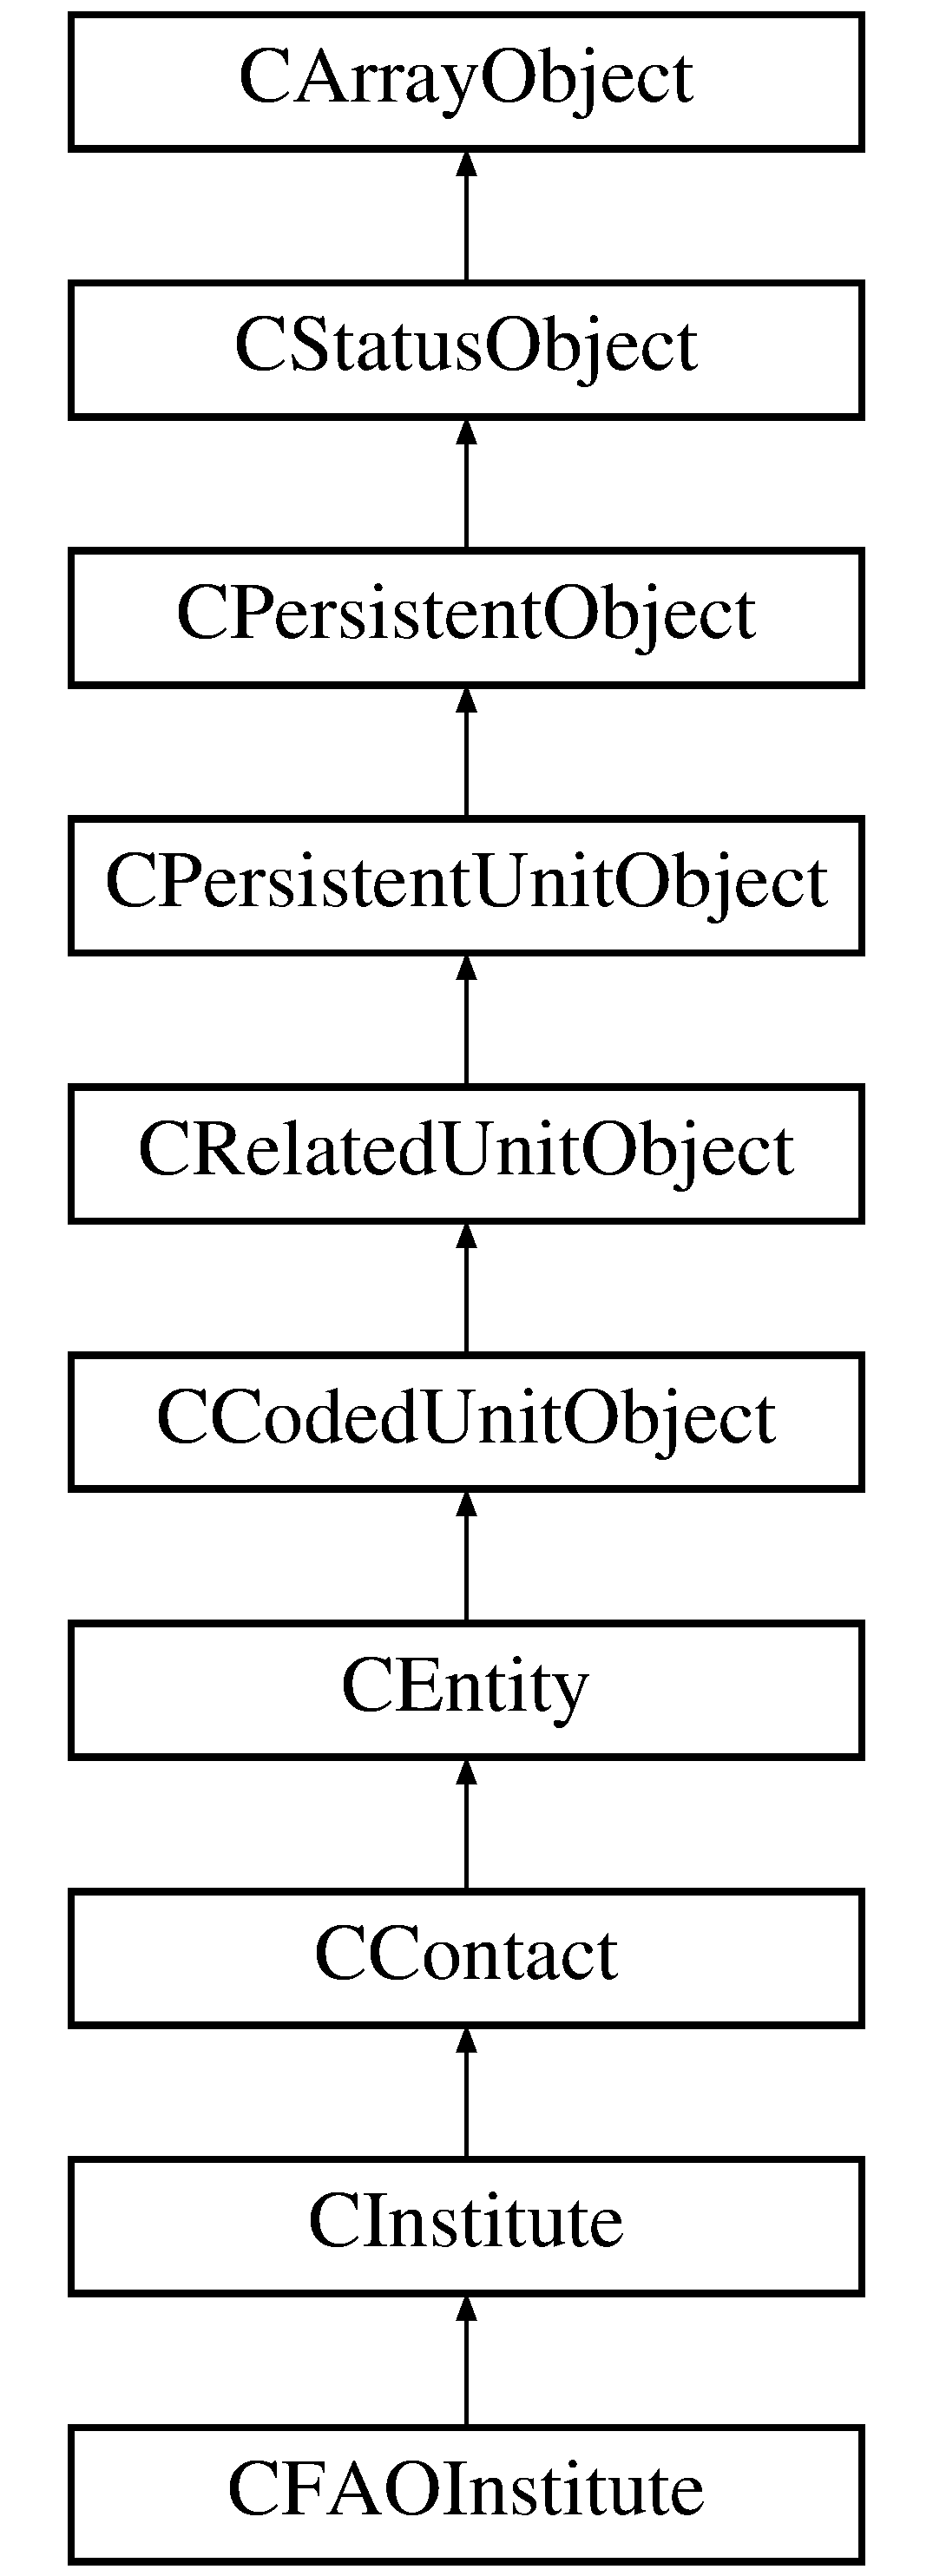
\includegraphics[height=10.000000cm]{class_c_f_a_o_institute}
\end{center}
\end{figure}
\subsection*{Public Member Functions}
\begin{DoxyCompactItemize}
\item 
\hyperlink{class_c_f_a_o_institute_af95063ebfd051df61eb523c47348d0d7}{E\-Acronym} (\$the\-Value=N\-U\-L\-L, \$get\-Old=F\-A\-L\-S\-E)
\item 
\hyperlink{class_c_f_a_o_institute_a6789e2ebcc8e919608aae8ec9956deb6}{F\-A\-O\-Type} (\$the\-Value=N\-U\-L\-L, \$the\-Operation=N\-U\-L\-L, \$get\-Old=F\-A\-L\-S\-E)
\item 
\hyperlink{class_c_f_a_o_institute_a861953952a7016f57759ef63045932f6}{Latitude} (\$the\-Value=N\-U\-L\-L, \$get\-Old=F\-A\-L\-S\-E)
\item 
\hyperlink{class_c_f_a_o_institute_a2adf396b5ecf8fd9eedcedc95a504f56}{Longitude} (\$the\-Value=N\-U\-L\-L, \$get\-Old=F\-A\-L\-S\-E)
\item 
\hyperlink{class_c_f_a_o_institute_a79db828d6210b8a21280e4edd3416935}{Altitude} (\$the\-Value=N\-U\-L\-L, \$get\-Old=F\-A\-L\-S\-E)
\item 
\hyperlink{class_c_f_a_o_institute_ac819c5bfa381ffa0f78b34442d2ea3c2}{offset\-Set} (\$the\-Offset, \$the\-Value)
\item 
\hyperlink{class_c_f_a_o_institute_a3bd7c59a3da53ba8c3cd1d9d0ff5ae0a}{offset\-Unset} (\$the\-Offset)
\end{DoxyCompactItemize}
\subsection*{Static Public Member Functions}
\begin{DoxyCompactItemize}
\item 
static \hyperlink{class_c_f_a_o_institute_abae6eb24454eb3824f5a89ccd1cbc808}{Import} (\$the\-Container, \$the\-U\-R\-L=k\-E\-N\-T\-I\-T\-Y\-\_\-\-I\-N\-S\-T\-\_\-\-F\-A\-O\-\_\-\-D\-O\-W\-N\-L\-O\-A\-D)
\item 
static \hyperlink{class_c_f_a_o_institute_ad9004a3928ad07bdac2988f48c5a8cdd}{Hash\-Index} (\$the\-Value)
\end{DoxyCompactItemize}
\subsection*{Protected Member Functions}
\begin{DoxyCompactItemize}
\item 
\hyperlink{class_c_f_a_o_institute_a9917150b0e31b741aa10c9443e880746}{\-\_\-\-Prepare\-Commit} (\&\$the\-Container, \&\$the\-Identifier, \&\$the\-Modifiers)
\end{DoxyCompactItemize}


\subsection{Member Function Documentation}
\hypertarget{class_c_f_a_o_institute_a9917150b0e31b741aa10c9443e880746}{\index{C\-F\-A\-O\-Institute@{C\-F\-A\-O\-Institute}!\-\_\-\-Prepare\-Commit@{\-\_\-\-Prepare\-Commit}}
\index{\-\_\-\-Prepare\-Commit@{\-\_\-\-Prepare\-Commit}!CFAOInstitute@{C\-F\-A\-O\-Institute}}
\subsubsection[{\-\_\-\-Prepare\-Commit}]{\setlength{\rightskip}{0pt plus 5cm}C\-F\-A\-O\-Institute\-::\-\_\-\-Prepare\-Commit (
\begin{DoxyParamCaption}
\item[{\&}]{\$the\-Container, }
\item[{\&}]{\$the\-Identifier, }
\item[{\&}]{\$the\-Modifiers}
\end{DoxyParamCaption}
)\hspace{0.3cm}{\ttfamily [protected]}}}\label{class_c_f_a_o_institute_a9917150b0e31b741aa10c9443e880746}
Normalise parameters of a store.

We overload this method to add the \hyperlink{}{k\-E\-N\-T\-I\-T\-Y\-\_\-\-I\-N\-S\-T\-\_\-\-F\-A\-O} \hyperlink{}{type} to the object prior \hyperlink{class_c_persistent_object_a88b1f2b11d3d60e0b3d33d8b0649b68a}{saving} it.


\begin{DoxyParams}[1]{Parameters}
reference & {\em \&\$the\-Container} & Object container. \\
\hline
reference & {\em \&\$the\-Identifier} & Object identifier. \\
\hline
reference & {\em \&\$the\-Modifiers} & Commit modifiers.\\
\hline
\end{DoxyParams}
protected


\begin{DoxyExceptions}{Exceptions}
{\em \{@link} & \hyperlink{class_c_exception}{C\-Exception} \hyperlink{class_c_exception}{C\-Exception}\}\\
\hline
\end{DoxyExceptions}
\begin{DoxySeeAlso}{See also}
k\-E\-R\-R\-O\-R\-\_\-\-O\-P\-T\-I\-O\-N\-\_\-\-M\-I\-S\-S\-I\-N\-G 
\end{DoxySeeAlso}


Reimplemented from \hyperlink{class_c_institute_a096aa38309ae2f88250700d5755a18a6}{C\-Institute}.

\hypertarget{class_c_f_a_o_institute_a79db828d6210b8a21280e4edd3416935}{\index{C\-F\-A\-O\-Institute@{C\-F\-A\-O\-Institute}!Altitude@{Altitude}}
\index{Altitude@{Altitude}!CFAOInstitute@{C\-F\-A\-O\-Institute}}
\subsubsection[{Altitude}]{\setlength{\rightskip}{0pt plus 5cm}C\-F\-A\-O\-Institute\-::\-Altitude (
\begin{DoxyParamCaption}
\item[{}]{\$the\-Value = {\ttfamily NULL}, }
\item[{}]{\$get\-Old = {\ttfamily FALSE}}
\end{DoxyParamCaption}
)}}\label{class_c_f_a_o_institute_a79db828d6210b8a21280e4edd3416935}
Manage institute altitude.

This method can be used to handle the institute \hyperlink{}{altitude}, it uses the standard accessor \hyperlink{class_c_attribute_a9d231a47718719fcd6c33f3d0ac91675}{method} to manage the \hyperlink{}{offset}.

This value is provided as an integer, specialised classes may convert it.

For a more in-\/depth reference of this method, please consult the \hyperlink{class_c_attribute_a9d231a47718719fcd6c33f3d0ac91675}{C\-Attribute\-::\-Manage\-Offset} method, in which the second parameter will be the constant \hyperlink{}{k\-E\-N\-T\-I\-T\-Y\-\_\-\-I\-N\-S\-T\-\_\-\-F\-A\-O\-\_\-\-A\-L\-T}.


\begin{DoxyParams}[1]{Parameters}
mixed & {\em \$the\-Value} & Value. \\
\hline
boolean & {\em \$get\-Old} & T\-R\-U\-E get old value.\\
\hline
\end{DoxyParams}
public \begin{DoxyReturn}{Returns}
string
\end{DoxyReturn}
\hyperlink{class_c_attribute_a9d231a47718719fcd6c33f3d0ac91675}{C\-Attribute\-::\-Manage\-Offset()}

\begin{DoxySeeAlso}{See also}
k\-E\-N\-T\-I\-T\-Y\-\_\-\-I\-N\-S\-T\-\_\-\-F\-A\-O\-\_\-\-A\-L\-T 
\end{DoxySeeAlso}
\hypertarget{class_c_f_a_o_institute_af95063ebfd051df61eb523c47348d0d7}{\index{C\-F\-A\-O\-Institute@{C\-F\-A\-O\-Institute}!E\-Acronym@{E\-Acronym}}
\index{E\-Acronym@{E\-Acronym}!CFAOInstitute@{C\-F\-A\-O\-Institute}}
\subsubsection[{E\-Acronym}]{\setlength{\rightskip}{0pt plus 5cm}C\-F\-A\-O\-Institute\-::\-E\-Acronym (
\begin{DoxyParamCaption}
\item[{}]{\$the\-Value = {\ttfamily NULL}, }
\item[{}]{\$get\-Old = {\ttfamily FALSE}}
\end{DoxyParamCaption}
)}}\label{class_c_f_a_o_institute_af95063ebfd051df61eb523c47348d0d7}
Manage institute E\-C\-P\-G\-R acronym.

This method can be used to handle the institute E\-C\-P\-G\-R \hyperlink{}{acronym}, it uses the standard accessor \hyperlink{class_c_attribute_a9d231a47718719fcd6c33f3d0ac91675}{method} to manage the \hyperlink{}{offset}.

This value should be a string.

For a more in-\/depth reference of this method, please consult the \hyperlink{class_c_attribute_a9d231a47718719fcd6c33f3d0ac91675}{C\-Attribute\-::\-Manage\-Offset} method, in which the second parameter will be the constant \hyperlink{}{k\-E\-N\-T\-I\-T\-Y\-\_\-\-I\-N\-S\-T\-\_\-\-F\-A\-O\-\_\-\-E\-P\-A\-C\-R\-O\-N\-Y\-M}.


\begin{DoxyParams}[1]{Parameters}
mixed & {\em \$the\-Value} & Value. \\
\hline
boolean & {\em \$get\-Old} & T\-R\-U\-E get old value.\\
\hline
\end{DoxyParams}
public \begin{DoxyReturn}{Returns}
string
\end{DoxyReturn}
\hyperlink{class_c_attribute_a9d231a47718719fcd6c33f3d0ac91675}{C\-Attribute\-::\-Manage\-Offset()}

\begin{DoxySeeAlso}{See also}
k\-E\-N\-T\-I\-T\-Y\-\_\-\-I\-N\-S\-T\-\_\-\-F\-A\-O\-\_\-\-E\-P\-A\-C\-R\-O\-N\-Y\-M 
\end{DoxySeeAlso}
\hypertarget{class_c_f_a_o_institute_a6789e2ebcc8e919608aae8ec9956deb6}{\index{C\-F\-A\-O\-Institute@{C\-F\-A\-O\-Institute}!F\-A\-O\-Type@{F\-A\-O\-Type}}
\index{F\-A\-O\-Type@{F\-A\-O\-Type}!CFAOInstitute@{C\-F\-A\-O\-Institute}}
\subsubsection[{F\-A\-O\-Type}]{\setlength{\rightskip}{0pt plus 5cm}C\-F\-A\-O\-Institute\-::\-F\-A\-O\-Type (
\begin{DoxyParamCaption}
\item[{}]{\$the\-Value = {\ttfamily NULL}, }
\item[{}]{\$the\-Operation = {\ttfamily NULL}, }
\item[{}]{\$get\-Old = {\ttfamily FALSE}}
\end{DoxyParamCaption}
)}}\label{class_c_f_a_o_institute_a6789e2ebcc8e919608aae8ec9956deb6}
Manage F\-A\-O/\-W\-I\-E\-W\-S types.

This method can be used to handle the institute F\-A\-O/\-W\-I\-E\-W\-S \hyperlink{}{types} list, it uses the standard accessor \hyperlink{class_c_attribute_a7d2e35b120eaa55529f78253f77dab48}{method} to manage the list of acronyms.

Each element of this list should indicate an acronym by which one refers to the current institute, the nature and specifics of these elements is the responsibility of concrete classes.

For a more thorough reference of how this method works, please consult the \hyperlink{class_c_attribute_a7d2e35b120eaa55529f78253f77dab48}{C\-Attribute\-::\-Manage\-Array\-Offset} method, in which the second parameter will be the constant \hyperlink{}{k\-E\-N\-T\-I\-T\-Y\-\_\-\-I\-N\-S\-T\-\_\-\-F\-A\-O\-\_\-\-T\-Y\-P\-E}.


\begin{DoxyParams}[1]{Parameters}
mixed & {\em \$the\-Value} & Value or index. \\
\hline
mixed & {\em \$the\-Operation} & Operation. \\
\hline
boolean & {\em \$get\-Old} & T\-R\-U\-E get old value.\\
\hline
\end{DoxyParams}
public \begin{DoxyReturn}{Returns}
mixed
\end{DoxyReturn}
\hyperlink{class_c_attribute_a7d2e35b120eaa55529f78253f77dab48}{C\-Attribute\-::\-Manage\-Array\-Offset()}

\begin{DoxySeeAlso}{See also}
k\-E\-N\-T\-I\-T\-Y\-\_\-\-I\-N\-S\-T\-\_\-\-F\-A\-O\-\_\-\-T\-Y\-P\-E 
\end{DoxySeeAlso}
\hypertarget{class_c_f_a_o_institute_ad9004a3928ad07bdac2988f48c5a8cdd}{\index{C\-F\-A\-O\-Institute@{C\-F\-A\-O\-Institute}!Hash\-Index@{Hash\-Index}}
\index{Hash\-Index@{Hash\-Index}!CFAOInstitute@{C\-F\-A\-O\-Institute}}
\subsubsection[{Hash\-Index}]{\setlength{\rightskip}{0pt plus 5cm}static C\-F\-A\-O\-Institute\-::\-Hash\-Index (
\begin{DoxyParamCaption}
\item[{}]{\$the\-Value}
\end{DoxyParamCaption}
)\hspace{0.3cm}{\ttfamily [static]}}}\label{class_c_f_a_o_institute_ad9004a3928ad07bdac2988f48c5a8cdd}
Hash index.

In this class we do not nodify the provided value, it is supposed to be the F\-A\-O institute {\itshape I\-N\-S\-T\-C\-O\-D\-E} field.


\begin{DoxyParams}[1]{Parameters}
string & {\em \$the\-Value} & Value to hash.\\
\hline
\end{DoxyParams}
\begin{DoxyReturn}{Returns}
string 
\end{DoxyReturn}


Reimplemented from \hyperlink{class_c_institute_a7a6915d35bc47272faabe8111574dddc}{C\-Institute}.

\hypertarget{class_c_f_a_o_institute_abae6eb24454eb3824f5a89ccd1cbc808}{\index{C\-F\-A\-O\-Institute@{C\-F\-A\-O\-Institute}!Import@{Import}}
\index{Import@{Import}!CFAOInstitute@{C\-F\-A\-O\-Institute}}
\subsubsection[{Import}]{\setlength{\rightskip}{0pt plus 5cm}static C\-F\-A\-O\-Institute\-::\-Import (
\begin{DoxyParamCaption}
\item[{}]{\$the\-Container, }
\item[{}]{\$the\-U\-R\-L = {\ttfamily kENTITY\-\_\-INST\-\_\-FAO\-\_\-DOWNLOAD}}
\end{DoxyParamCaption}
)\hspace{0.3cm}{\ttfamily [static]}}}\label{class_c_f_a_o_institute_abae6eb24454eb3824f5a89ccd1cbc808}
Import institutes.

This method can be used to import the institutes list from the current F\-A\-O/\-W\-I\-E\-W\-S export file, the method expects two parameters\-:


\begin{DoxyItemize}
\item {\bfseries \$the\-Container}\-: The \hyperlink{class_c_container}{container} in which the institutes are stored. 
\item {\bfseries \$the\-U\-R\-L}\-: The download U\-R\-L of the F\-A\-O/\-W\-I\-E\-W\-S export file. 
\end{DoxyItemize}

The method will return the number of records added and replaced.

{\itshape Note that the method will commit the records using the \hyperlink{}{k\-F\-L\-A\-G\-\_\-\-P\-E\-R\-S\-I\-S\-T\-\_\-\-R\-E\-P\-L\-A\-C\-E} and \hyperlink{}{k\-F\-L\-A\-G\-\_\-\-S\-T\-A\-T\-E\-\_\-\-E\-N\-C\-O\-D\-E\-D} flags}.


\begin{DoxyParams}[1]{Parameters}
\hyperlink{class_c_container}{C\-Container} & {\em \$the\-Container} & Data container. \\
\hline
string & {\em \$the\-U\-R\-L} & Import file path.\\
\hline
\end{DoxyParams}
\begin{DoxyReturn}{Returns}
integer 
\end{DoxyReturn}
\hypertarget{class_c_f_a_o_institute_a861953952a7016f57759ef63045932f6}{\index{C\-F\-A\-O\-Institute@{C\-F\-A\-O\-Institute}!Latitude@{Latitude}}
\index{Latitude@{Latitude}!CFAOInstitute@{C\-F\-A\-O\-Institute}}
\subsubsection[{Latitude}]{\setlength{\rightskip}{0pt plus 5cm}C\-F\-A\-O\-Institute\-::\-Latitude (
\begin{DoxyParamCaption}
\item[{}]{\$the\-Value = {\ttfamily NULL}, }
\item[{}]{\$get\-Old = {\ttfamily FALSE}}
\end{DoxyParamCaption}
)}}\label{class_c_f_a_o_institute_a861953952a7016f57759ef63045932f6}
Manage institute latitude.

This method can be used to handle the institute \hyperlink{}{latitude}, it uses the standard accessor \hyperlink{class_c_attribute_a9d231a47718719fcd6c33f3d0ac91675}{method} to manage the \hyperlink{}{offset}.

This value is provided as an integer, specialised classes may convert it.

For a more in-\/depth reference of this method, please consult the \hyperlink{class_c_attribute_a9d231a47718719fcd6c33f3d0ac91675}{C\-Attribute\-::\-Manage\-Offset} method, in which the second parameter will be the constant \hyperlink{}{k\-E\-N\-T\-I\-T\-Y\-\_\-\-I\-N\-S\-T\-\_\-\-F\-A\-O\-\_\-\-L\-A\-T}.


\begin{DoxyParams}[1]{Parameters}
mixed & {\em \$the\-Value} & Value. \\
\hline
boolean & {\em \$get\-Old} & T\-R\-U\-E get old value.\\
\hline
\end{DoxyParams}
public \begin{DoxyReturn}{Returns}
string
\end{DoxyReturn}
\hyperlink{class_c_attribute_a9d231a47718719fcd6c33f3d0ac91675}{C\-Attribute\-::\-Manage\-Offset()}

\begin{DoxySeeAlso}{See also}
k\-E\-N\-T\-I\-T\-Y\-\_\-\-I\-N\-S\-T\-\_\-\-F\-A\-O\-\_\-\-L\-A\-T 
\end{DoxySeeAlso}
\hypertarget{class_c_f_a_o_institute_a2adf396b5ecf8fd9eedcedc95a504f56}{\index{C\-F\-A\-O\-Institute@{C\-F\-A\-O\-Institute}!Longitude@{Longitude}}
\index{Longitude@{Longitude}!CFAOInstitute@{C\-F\-A\-O\-Institute}}
\subsubsection[{Longitude}]{\setlength{\rightskip}{0pt plus 5cm}C\-F\-A\-O\-Institute\-::\-Longitude (
\begin{DoxyParamCaption}
\item[{}]{\$the\-Value = {\ttfamily NULL}, }
\item[{}]{\$get\-Old = {\ttfamily FALSE}}
\end{DoxyParamCaption}
)}}\label{class_c_f_a_o_institute_a2adf396b5ecf8fd9eedcedc95a504f56}
Manage institute longitude.

This method can be used to handle the institute \hyperlink{}{longitude}, it uses the standard accessor \hyperlink{class_c_attribute_a9d231a47718719fcd6c33f3d0ac91675}{method} to manage the \hyperlink{}{offset}.

This value is provided as an integer, specialised classes may convert it.

For a more in-\/depth reference of this method, please consult the \hyperlink{class_c_attribute_a9d231a47718719fcd6c33f3d0ac91675}{C\-Attribute\-::\-Manage\-Offset} method, in which the second parameter will be the constant \hyperlink{}{k\-E\-N\-T\-I\-T\-Y\-\_\-\-I\-N\-S\-T\-\_\-\-F\-A\-O\-\_\-\-L\-O\-N}.


\begin{DoxyParams}[1]{Parameters}
mixed & {\em \$the\-Value} & Value. \\
\hline
boolean & {\em \$get\-Old} & T\-R\-U\-E get old value.\\
\hline
\end{DoxyParams}
public \begin{DoxyReturn}{Returns}
string
\end{DoxyReturn}
\hyperlink{class_c_attribute_a9d231a47718719fcd6c33f3d0ac91675}{C\-Attribute\-::\-Manage\-Offset()}

\begin{DoxySeeAlso}{See also}
k\-E\-N\-T\-I\-T\-Y\-\_\-\-I\-N\-S\-T\-\_\-\-F\-A\-O\-\_\-\-L\-O\-N 
\end{DoxySeeAlso}
\hypertarget{class_c_f_a_o_institute_ac819c5bfa381ffa0f78b34442d2ea3c2}{\index{C\-F\-A\-O\-Institute@{C\-F\-A\-O\-Institute}!offset\-Set@{offset\-Set}}
\index{offset\-Set@{offset\-Set}!CFAOInstitute@{C\-F\-A\-O\-Institute}}
\subsubsection[{offset\-Set}]{\setlength{\rightskip}{0pt plus 5cm}C\-F\-A\-O\-Institute\-::offset\-Set (
\begin{DoxyParamCaption}
\item[{}]{\$the\-Offset, }
\item[{}]{\$the\-Value}
\end{DoxyParamCaption}
)}}\label{class_c_f_a_o_institute_ac819c5bfa381ffa0f78b34442d2ea3c2}
Set a value for a given offset.

We overload this method to override the \hyperlink{class_c_status_object_a8429102e4f52f7558649b64f4e673a69}{inited} \hyperlink{}{status} of the \hyperlink{class_c_institute}{parent} class\-: F\-A\-O institutes may not have a \hyperlink{class_c_entity_ace5878c009baf09d85c8ca115c48dbb0}{name} set, so we call the \hyperlink{class_c_entity}{entity} version of this method.


\begin{DoxyParams}[1]{Parameters}
string & {\em \$the\-Offset} & Offset. \\
\hline
string | N\-U\-L\-L & {\em \$the\-Value} & Value to set at offset.\\
\hline
\end{DoxyParams}
public 

Reimplemented from \hyperlink{class_c_institute_a16c349e22775161c89dbf73850b24cd7}{C\-Institute}.

\hypertarget{class_c_f_a_o_institute_a3bd7c59a3da53ba8c3cd1d9d0ff5ae0a}{\index{C\-F\-A\-O\-Institute@{C\-F\-A\-O\-Institute}!offset\-Unset@{offset\-Unset}}
\index{offset\-Unset@{offset\-Unset}!CFAOInstitute@{C\-F\-A\-O\-Institute}}
\subsubsection[{offset\-Unset}]{\setlength{\rightskip}{0pt plus 5cm}C\-F\-A\-O\-Institute\-::offset\-Unset (
\begin{DoxyParamCaption}
\item[{}]{\$the\-Offset}
\end{DoxyParamCaption}
)}}\label{class_c_f_a_o_institute_a3bd7c59a3da53ba8c3cd1d9d0ff5ae0a}
Reset a value for a given offset.

We overload this method to override the \hyperlink{class_c_status_object_a8429102e4f52f7558649b64f4e673a69}{inited} \hyperlink{}{status} of the \hyperlink{class_c_institute}{parent} class\-: F\-A\-O institutes may not have a \hyperlink{class_c_entity_ace5878c009baf09d85c8ca115c48dbb0}{name} set, so we call the \hyperlink{class_c_entity}{entity} version of this method.


\begin{DoxyParams}[1]{Parameters}
string & {\em \$the\-Offset} & Offset.\\
\hline
\end{DoxyParams}
public 

Reimplemented from \hyperlink{class_c_institute_a8f82ded3b52a6fb609c67e45669e1454}{C\-Institute}.



The documentation for this class was generated from the following file\-:\begin{DoxyCompactItemize}
\item 
/\-Library/\-Web\-Server/\-Library/wrapper/classes/C\-F\-A\-O\-Institute.\-php\end{DoxyCompactItemize}

\hypertarget{class_c_graph_edge}{\section{C\-Graph\-Edge Class Reference}
\label{class_c_graph_edge}\index{C\-Graph\-Edge@{C\-Graph\-Edge}}
}
Inheritance diagram for C\-Graph\-Edge\-:\begin{figure}[H]
\begin{center}
\leavevmode
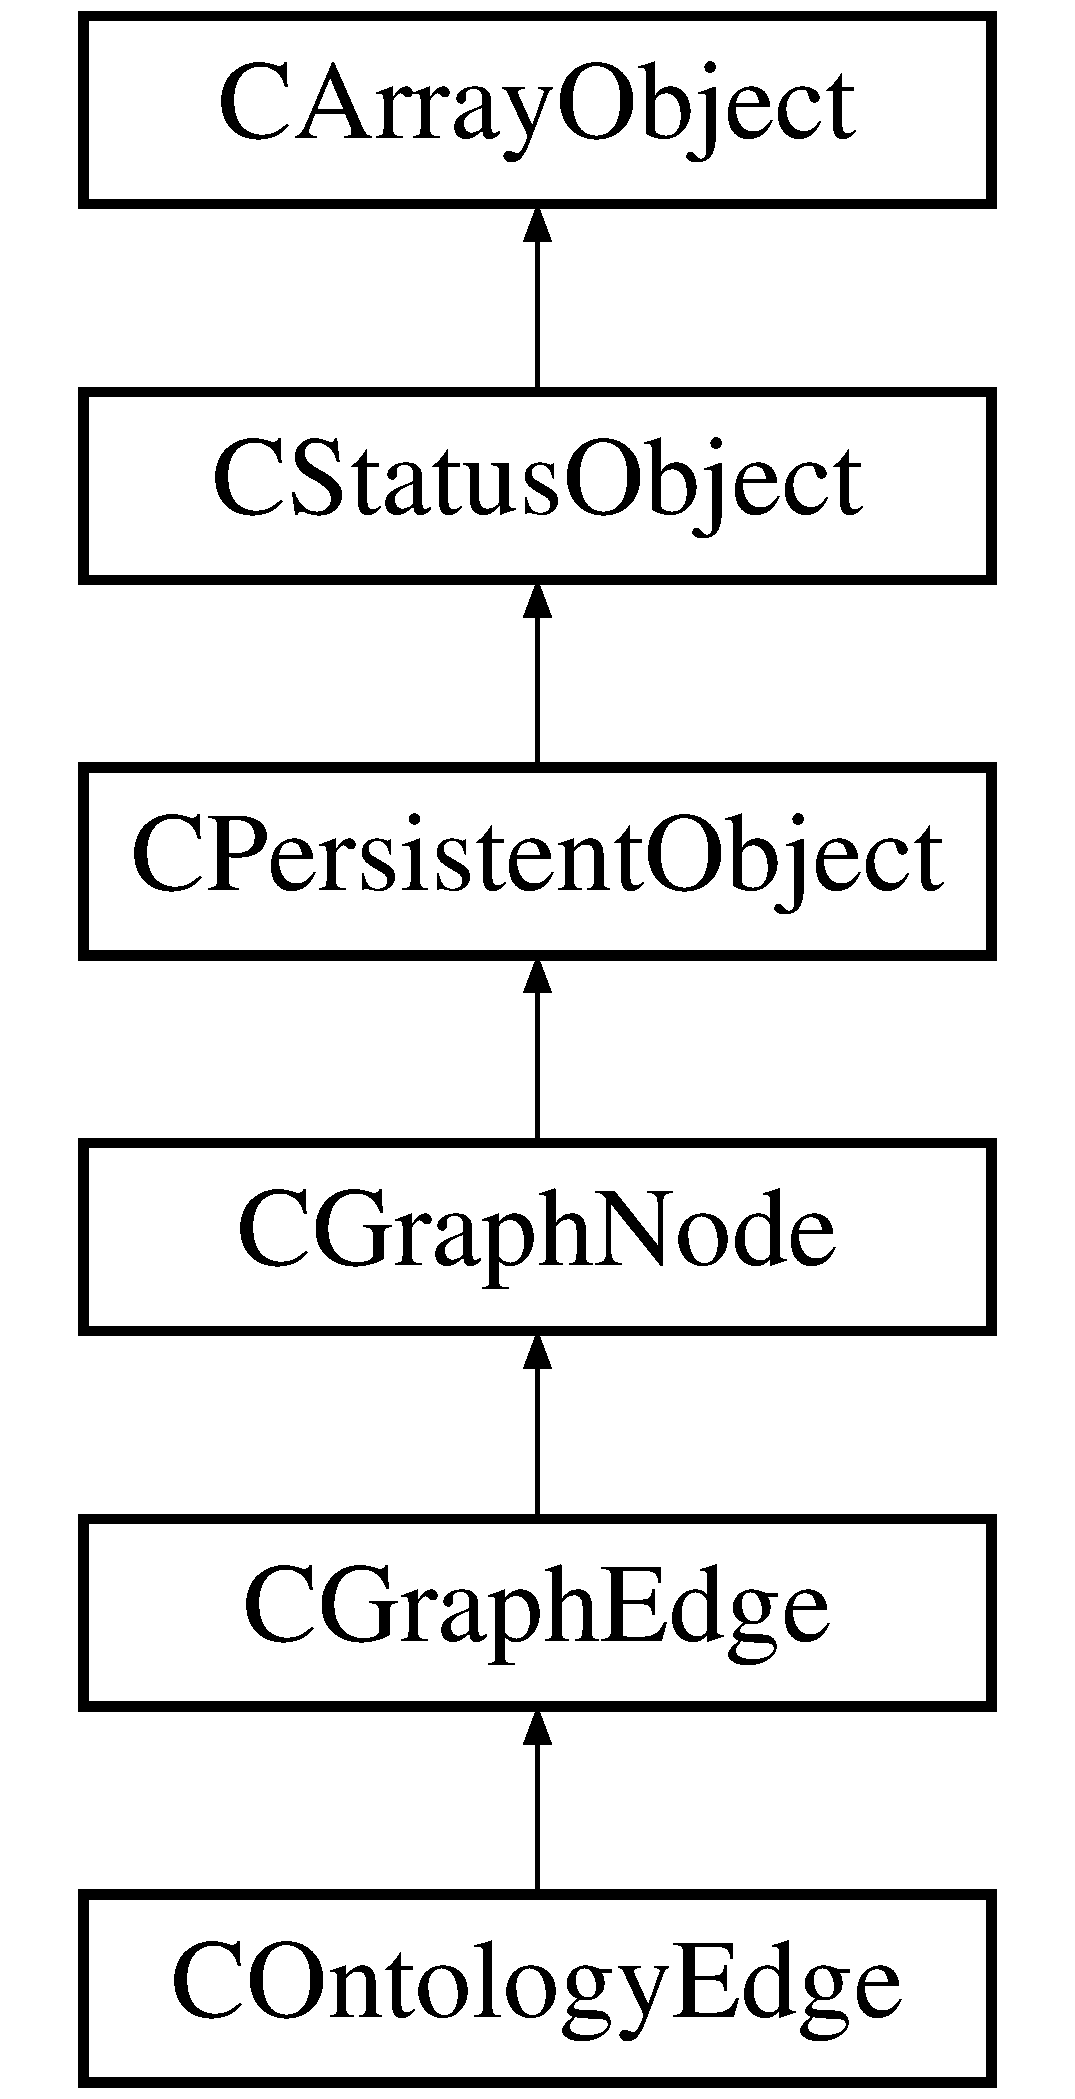
\includegraphics[height=6.000000cm]{class_c_graph_edge}
\end{center}
\end{figure}
\subsection*{Public Member Functions}
\begin{DoxyCompactItemize}
\item 
\hyperlink{class_c_graph_edge_a8329f594ad1ca48e5f1ccb04e02fdffb}{\-\_\-\-\_\-to\-String} ()
\item 
\hyperlink{class_c_graph_edge_a584c0263fd773ffb764385a51d36caf2}{Type} (\$the\-Value=N\-U\-L\-L, \$get\-Old=F\-A\-L\-S\-E)
\item 
\hyperlink{class_c_graph_edge_a6606e13ba79ab94fc0db50bef197d416}{Node} (\$the\-Value=N\-U\-L\-L, \$get\-Old=F\-A\-L\-S\-E)
\item 
\hyperlink{class_c_graph_edge_a85669389df602d0ed4f936824756f715}{Subject} (\$the\-Value=N\-U\-L\-L, \$get\-Old=F\-A\-L\-S\-E)
\item 
\hyperlink{class_c_graph_edge_a6714cb916eaf902979eb84590b337cf9}{Object} (\$the\-Value=N\-U\-L\-L, \$get\-Old=F\-A\-L\-S\-E)
\end{DoxyCompactItemize}
\subsection*{Protected Member Functions}
\begin{DoxyCompactItemize}
\item 
\hyperlink{class_c_graph_edge_a73dd2ced3103285f8ad4ea212c0e918e}{\-\_\-\-Commit} (\&\$the\-Container, \&\$the\-Identifier, \&\$the\-Modifiers)
\item 
\hyperlink{class_c_graph_edge_a8c19599c8543c9c1a25b9c2dfba8e223}{\-\_\-\-Load} (\&\$the\-Container, \&\$the\-Identifier, \&\$the\-Modifiers)
\item 
\hyperlink{class_c_graph_edge_a42fd83eff1eef079a6005e961fd2d371}{\-\_\-\-Finish\-Create} (\&\$the\-Container)
\item 
\hyperlink{class_c_graph_edge_a7cbf3dab4745b0924905fce01e383819}{\-\_\-\-Finish\-Load} (\&\$the\-Container, \&\$the\-Identifier, \&\$the\-Modifiers)
\end{DoxyCompactItemize}
\subsection*{Additional Inherited Members}


\subsection{Member Function Documentation}
\hypertarget{class_c_graph_edge_a8329f594ad1ca48e5f1ccb04e02fdffb}{\index{C\-Graph\-Edge@{C\-Graph\-Edge}!\-\_\-\-\_\-to\-String@{\-\_\-\-\_\-to\-String}}
\index{\-\_\-\-\_\-to\-String@{\-\_\-\-\_\-to\-String}!CGraphEdge@{C\-Graph\-Edge}}
\subsubsection[{\-\_\-\-\_\-to\-String}]{\setlength{\rightskip}{0pt plus 5cm}C\-Graph\-Edge\-::\-\_\-\-\_\-to\-String (
\begin{DoxyParamCaption}
{}
\end{DoxyParamCaption}
)}}\label{class_c_graph_edge_a8329f594ad1ca48e5f1ccb04e02fdffb}
Return object identifier.

In this class we return the graph \hyperlink{class_c_graph_edge_a584c0263fd773ffb764385a51d36caf2}{type}.

public \begin{DoxyReturn}{Returns}
string
\end{DoxyReturn}
\hyperlink{class_c_graph_edge_a584c0263fd773ffb764385a51d36caf2}{Type()} 

Reimplemented from \hyperlink{class_c_graph_node_a59905bb321a3fb6a1540a6ffba12f2a0}{C\-Graph\-Node}.

\hypertarget{class_c_graph_edge_a73dd2ced3103285f8ad4ea212c0e918e}{\index{C\-Graph\-Edge@{C\-Graph\-Edge}!\-\_\-\-Commit@{\-\_\-\-Commit}}
\index{\-\_\-\-Commit@{\-\_\-\-Commit}!CGraphEdge@{C\-Graph\-Edge}}
\subsubsection[{\-\_\-\-Commit}]{\setlength{\rightskip}{0pt plus 5cm}C\-Graph\-Edge\-::\-\_\-\-Commit (
\begin{DoxyParamCaption}
\item[{\&}]{\$the\-Container, }
\item[{\&}]{\$the\-Identifier, }
\item[{\&}]{\$the\-Modifiers}
\end{DoxyParamCaption}
)\hspace{0.3cm}{\ttfamily [protected]}}}\label{class_c_graph_edge_a73dd2ced3103285f8ad4ea212c0e918e}
Store object in container.

We \hyperlink{class_c_graph_node_a7af17771eaba24551f8c9a465f391c23}{override} this method to initialise an empty relationship rather than a node when deleting.


\begin{DoxyParams}[1]{Parameters}
reference & {\em \&\$the\-Container} & Object container. \\
\hline
reference & {\em \&\$the\-Identifier} & Object identifier. \\
\hline
reference & {\em \&\$the\-Modifiers} & Commit modifiers.\\
\hline
\end{DoxyParams}
protected \begin{DoxyReturn}{Returns}
mixed
\end{DoxyReturn}
\hyperlink{class_c_graph_edge_a6606e13ba79ab94fc0db50bef197d416}{Node()} 

Reimplemented from \hyperlink{class_c_graph_node_a7af17771eaba24551f8c9a465f391c23}{C\-Graph\-Node}.



Reimplemented in \hyperlink{class_c_ontology_edge_a76e551f21dcac3c0bc228c67226bec08}{C\-Ontology\-Edge}.

\hypertarget{class_c_graph_edge_a42fd83eff1eef079a6005e961fd2d371}{\index{C\-Graph\-Edge@{C\-Graph\-Edge}!\-\_\-\-Finish\-Create@{\-\_\-\-Finish\-Create}}
\index{\-\_\-\-Finish\-Create@{\-\_\-\-Finish\-Create}!CGraphEdge@{C\-Graph\-Edge}}
\subsubsection[{\-\_\-\-Finish\-Create}]{\setlength{\rightskip}{0pt plus 5cm}C\-Graph\-Edge\-::\-\_\-\-Finish\-Create (
\begin{DoxyParamCaption}
\item[{\&}]{\$the\-Container}
\end{DoxyParamCaption}
)\hspace{0.3cm}{\ttfamily [protected]}}}\label{class_c_graph_edge_a42fd83eff1eef079a6005e961fd2d371}
Normalise after a \hyperlink{class_c_graph_node_a90e49bf5e95ccf3c8644196696154268}{create}.

We \hyperlink{class_c_graph_node_a8a8df45cff2375d0bcbb15342ae3960b}{override} this method to handle relationships rather than nodes, and to initialise related nodes.


\begin{DoxyParams}[1]{Parameters}
reference & {\em \&\$the\-Container} & Object container.\\
\hline
\end{DoxyParams}
protected 

Reimplemented from \hyperlink{class_c_graph_node_a8a8df45cff2375d0bcbb15342ae3960b}{C\-Graph\-Node}.



Reimplemented in \hyperlink{class_c_ontology_edge_a0956d5920484a329c77d878bb6c25784}{C\-Ontology\-Edge}.

\hypertarget{class_c_graph_edge_a7cbf3dab4745b0924905fce01e383819}{\index{C\-Graph\-Edge@{C\-Graph\-Edge}!\-\_\-\-Finish\-Load@{\-\_\-\-Finish\-Load}}
\index{\-\_\-\-Finish\-Load@{\-\_\-\-Finish\-Load}!CGraphEdge@{C\-Graph\-Edge}}
\subsubsection[{\-\_\-\-Finish\-Load}]{\setlength{\rightskip}{0pt plus 5cm}C\-Graph\-Edge\-::\-\_\-\-Finish\-Load (
\begin{DoxyParamCaption}
\item[{\&}]{\$the\-Container, }
\item[{\&}]{\$the\-Identifier, }
\item[{\&}]{\$the\-Modifiers}
\end{DoxyParamCaption}
)\hspace{0.3cm}{\ttfamily [protected]}}}\label{class_c_graph_edge_a7cbf3dab4745b0924905fce01e383819}
Normalise after a \hyperlink{class_c_graph_edge_a8c19599c8543c9c1a25b9c2dfba8e223}{load}.

We \hyperlink{class_c_graph_node_a8a8df45cff2375d0bcbb15342ae3960b}{override} this method to handle relationships rather than nodes.


\begin{DoxyParams}[1]{Parameters}
reference & {\em \&\$the\-Container} & Object container. \\
\hline
reference & {\em \&\$the\-Identifier} & Object identifier. \\
\hline
reference & {\em \&\$the\-Modifiers} & Create modifiers.\\
\hline
\end{DoxyParams}
protected 

Reimplemented from \hyperlink{class_c_graph_node_a23c2beb0fbed1ab67018dd9d78dee8fa}{C\-Graph\-Node}.



Reimplemented in \hyperlink{class_c_ontology_edge_ac45af3396c797be599c2a1780b7bfa59}{C\-Ontology\-Edge}.

\hypertarget{class_c_graph_edge_a8c19599c8543c9c1a25b9c2dfba8e223}{\index{C\-Graph\-Edge@{C\-Graph\-Edge}!\-\_\-\-Load@{\-\_\-\-Load}}
\index{\-\_\-\-Load@{\-\_\-\-Load}!CGraphEdge@{C\-Graph\-Edge}}
\subsubsection[{\-\_\-\-Load}]{\setlength{\rightskip}{0pt plus 5cm}C\-Graph\-Edge\-::\-\_\-\-Load (
\begin{DoxyParamCaption}
\item[{\&}]{\$the\-Container, }
\item[{\&}]{\$the\-Identifier, }
\item[{\&}]{\$the\-Modifiers}
\end{DoxyParamCaption}
)\hspace{0.3cm}{\ttfamily [protected]}}}\label{class_c_graph_edge_a8c19599c8543c9c1a25b9c2dfba8e223}
Find object.

We \hyperlink{class_c_graph_node_a7af17771eaba24551f8c9a465f391c23}{override} this method to locate relationships rather than nodes.


\begin{DoxyParams}[1]{Parameters}
reference & {\em \&\$the\-Container} & Object container. \\
\hline
reference & {\em \&\$the\-Identifier} & Object identifier. \\
\hline
reference & {\em \&\$the\-Modifiers} & Create options.\\
\hline
\end{DoxyParams}
protected \begin{DoxyReturn}{Returns}
mixed 
\end{DoxyReturn}


Reimplemented from \hyperlink{class_c_graph_node_a60c57e754245042fe04dad8fb63a5fec}{C\-Graph\-Node}.



Reimplemented in \hyperlink{class_c_ontology_edge_ae7a4861887c1a73dcdbd0285cdba1d8d}{C\-Ontology\-Edge}.

\hypertarget{class_c_graph_edge_a6606e13ba79ab94fc0db50bef197d416}{\index{C\-Graph\-Edge@{C\-Graph\-Edge}!Node@{Node}}
\index{Node@{Node}!CGraphEdge@{C\-Graph\-Edge}}
\subsubsection[{Node}]{\setlength{\rightskip}{0pt plus 5cm}C\-Graph\-Edge\-::\-Node (
\begin{DoxyParamCaption}
\item[{}]{\$the\-Value = {\ttfamily NULL}, }
\item[{}]{\$get\-Old = {\ttfamily FALSE}}
\end{DoxyParamCaption}
)}}\label{class_c_graph_edge_a6606e13ba79ab94fc0db50bef197d416}
Manage native node.

We override the \hyperlink{class_c_graph_node}{parent} \hyperlink{}{method} to enforce Everyman objects rather than Everyman objects.


\begin{DoxyParams}[1]{Parameters}
mixed & {\em \$the\-Value} & Node or operation. \\
\hline
boolean & {\em \$get\-Old} & T\-R\-U\-E get old value.\\
\hline
\end{DoxyParams}
public \begin{DoxyReturn}{Returns}
Everyman
\end{DoxyReturn}
\hyperlink{class_c_object_a9b8dccdadcf4fea58f915bd9b228e23e}{C\-Object\-::\-Manage\-Member()}  \hyperlink{class_c_status_object_a19c4ac94dfe26476e780d77b99744d43}{\-\_\-\-Is\-Dirty()}  \hyperlink{class_c_status_object_a8429102e4f52f7558649b64f4e673a69}{\-\_\-\-Is\-Inited()} 

Reimplemented from \hyperlink{class_c_graph_node_ad830025d2d6650006eb6e737bd4f32c0}{C\-Graph\-Node}.

\hypertarget{class_c_graph_edge_a6714cb916eaf902979eb84590b337cf9}{\index{C\-Graph\-Edge@{C\-Graph\-Edge}!Object@{Object}}
\index{Object@{Object}!CGraphEdge@{C\-Graph\-Edge}}
\subsubsection[{Object}]{\setlength{\rightskip}{0pt plus 5cm}C\-Graph\-Edge\-::\-Object (
\begin{DoxyParamCaption}
\item[{}]{\$the\-Value = {\ttfamily NULL}, }
\item[{}]{\$get\-Old = {\ttfamily FALSE}}
\end{DoxyParamCaption}
)}}\label{class_c_graph_edge_a6714cb916eaf902979eb84590b337cf9}
Manage object node.

This method will wrap the member accessor around the native relationship node, note that the method will not allow to delete a value, you must replace it.


\begin{DoxyItemize}
\item {\bfseries \$the\-Value}\-: The value or operation\-: 
\begin{DoxyItemize}
\item {\itshape N\-U\-L\-L}\-: Return the current value. 
\item {\itshape Everyman}\-: Set value. 
\item {\itshape other}\-: Raise exception. 
\end{DoxyItemize}
\item {\bfseries \$get\-Old}\-: Determines what the method will return\-: 
\begin{DoxyItemize}
\item {\itshape T\-R\-U\-E}\-: Return the value {\itshape before} it was eventually modified. 
\item {\itshape F\-A\-L\-S\-E}\-: Return the value {\itshape after} it was eventually modified. 
\end{DoxyItemize}
\end{DoxyItemize}


\begin{DoxyParams}[1]{Parameters}
mixed & {\em \$the\-Value} & Object node or operation. \\
\hline
boolean & {\em \$get\-Old} & T\-R\-U\-E get old value.\\
\hline
\end{DoxyParams}
public \begin{DoxyReturn}{Returns}
Everyman
\end{DoxyReturn}
\hyperlink{class_c_graph_edge_a6606e13ba79ab94fc0db50bef197d416}{Node()}  \hyperlink{class_c_status_object_a19c4ac94dfe26476e780d77b99744d43}{\-\_\-\-Is\-Dirty()}  \hyperlink{class_c_status_object_a8429102e4f52f7558649b64f4e673a69}{\-\_\-\-Is\-Inited()} \hypertarget{class_c_graph_edge_a85669389df602d0ed4f936824756f715}{\index{C\-Graph\-Edge@{C\-Graph\-Edge}!Subject@{Subject}}
\index{Subject@{Subject}!CGraphEdge@{C\-Graph\-Edge}}
\subsubsection[{Subject}]{\setlength{\rightskip}{0pt plus 5cm}C\-Graph\-Edge\-::\-Subject (
\begin{DoxyParamCaption}
\item[{}]{\$the\-Value = {\ttfamily NULL}, }
\item[{}]{\$get\-Old = {\ttfamily FALSE}}
\end{DoxyParamCaption}
)}}\label{class_c_graph_edge_a85669389df602d0ed4f936824756f715}
Manage subject node.

This method will wrap the member accessor around the native relationship node, note that the method will not allow to delete a value, you must replace it.


\begin{DoxyItemize}
\item {\bfseries \$the\-Value}\-: The value or operation\-: 
\begin{DoxyItemize}
\item {\itshape N\-U\-L\-L}\-: Return the current value. 
\item {\itshape Everyman}\-: Set value. 
\item {\itshape other}\-: Raise exception. 
\end{DoxyItemize}
\item {\bfseries \$get\-Old}\-: Determines what the method will return\-: 
\begin{DoxyItemize}
\item {\itshape T\-R\-U\-E}\-: Return the value {\itshape before} it was eventually modified. 
\item {\itshape F\-A\-L\-S\-E}\-: Return the value {\itshape after} it was eventually modified. 
\end{DoxyItemize}
\end{DoxyItemize}


\begin{DoxyParams}[1]{Parameters}
mixed & {\em \$the\-Value} & Subject node or operation. \\
\hline
boolean & {\em \$get\-Old} & T\-R\-U\-E get old value.\\
\hline
\end{DoxyParams}
public \begin{DoxyReturn}{Returns}
Everyman
\end{DoxyReturn}
\hyperlink{class_c_graph_edge_a6606e13ba79ab94fc0db50bef197d416}{Node()}  \hyperlink{class_c_status_object_a19c4ac94dfe26476e780d77b99744d43}{\-\_\-\-Is\-Dirty()}  \hyperlink{class_c_status_object_a8429102e4f52f7558649b64f4e673a69}{\-\_\-\-Is\-Inited()} \hypertarget{class_c_graph_edge_a584c0263fd773ffb764385a51d36caf2}{\index{C\-Graph\-Edge@{C\-Graph\-Edge}!Type@{Type}}
\index{Type@{Type}!CGraphEdge@{C\-Graph\-Edge}}
\subsubsection[{Type}]{\setlength{\rightskip}{0pt plus 5cm}C\-Graph\-Edge\-::\-Type (
\begin{DoxyParamCaption}
\item[{}]{\$the\-Value = {\ttfamily NULL}, }
\item[{}]{\$get\-Old = {\ttfamily FALSE}}
\end{DoxyParamCaption}
)}}\label{class_c_graph_edge_a584c0263fd773ffb764385a51d36caf2}
Manage node type.

This property corresponds to the node type, or predicate reference, this property is a string, and it is managed directly by the relationship node\-: we simply wrap this method around the native management\-:


\begin{DoxyItemize}
\item {\bfseries \$the\-Value}\-: The value or operation\-: 
\begin{DoxyItemize}
\item {\itshape N\-U\-L\-L}\-: Return the current value. 
\item {\itshape other}\-: Set the value converted to string. 
\end{DoxyItemize}
\item {\bfseries \$get\-Old}\-: Determines what the method will return\-: 
\begin{DoxyItemize}
\item {\itshape T\-R\-U\-E}\-: Return the value {\itshape before} it was eventually modified. 
\item {\itshape F\-A\-L\-S\-E}\-: Return the value {\itshape after} it was eventually modified. 
\end{DoxyItemize}
\end{DoxyItemize}


\begin{DoxyParams}[1]{Parameters}
mixed & {\em \$the\-Value} & Node or operation. \\
\hline
boolean & {\em \$get\-Old} & T\-R\-U\-E get old value.\\
\hline
\end{DoxyParams}
public \begin{DoxyReturn}{Returns}
string
\end{DoxyReturn}
\hyperlink{class_c_graph_edge_a6606e13ba79ab94fc0db50bef197d416}{Node()}  \hyperlink{class_c_status_object_a19c4ac94dfe26476e780d77b99744d43}{\-\_\-\-Is\-Dirty()}  \hyperlink{class_c_status_object_a8429102e4f52f7558649b64f4e673a69}{\-\_\-\-Is\-Inited()} 

The documentation for this class was generated from the following file\-:\begin{DoxyCompactItemize}
\item 
/\-Library/\-Web\-Server/\-Library/wrapper/classes/C\-Graph\-Edge.\-php\end{DoxyCompactItemize}

\hypertarget{class_c_graph_node}{\section{C\-Graph\-Node Class Reference}
\label{class_c_graph_node}\index{C\-Graph\-Node@{C\-Graph\-Node}}
}
Inheritance diagram for C\-Graph\-Node\-:\begin{figure}[H]
\begin{center}
\leavevmode
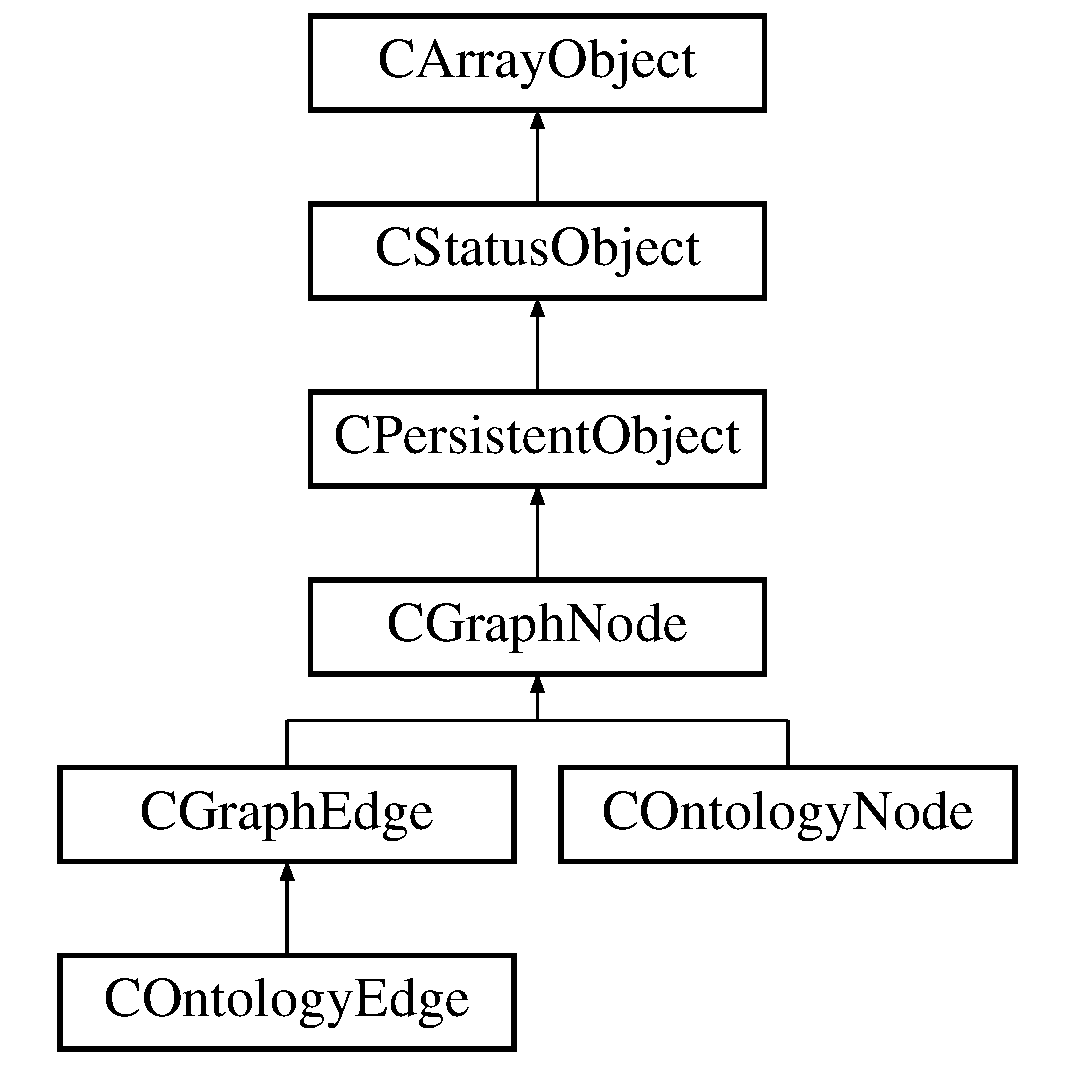
\includegraphics[height=6.000000cm]{class_c_graph_node}
\end{center}
\end{figure}
\subsection*{Public Member Functions}
\begin{DoxyCompactItemize}
\item 
\hyperlink{class_c_graph_node_a59905bb321a3fb6a1540a6ffba12f2a0}{\-\_\-\-\_\-to\-String} ()
\item 
\hyperlink{class_c_graph_node_ad830025d2d6650006eb6e737bd4f32c0}{Node} (\$the\-Value=N\-U\-L\-L, \$get\-Old=F\-A\-L\-S\-E)
\item 
\hyperlink{class_c_graph_node_a287e129b287f2479b7b23dc17b9fdac5}{Relate\-To} (\$the\-Container, \$the\-Predicate, \$the\-Object)
\item 
\hyperlink{class_c_graph_node_a2f2f02ee7ded7710e6f7533611ec638b}{Persistent} ()
\item 
\hyperlink{class_c_graph_node_a8c567e73a79cddc0e3582b3bd766d980}{offset\-Exists} (\$the\-Offset)
\item 
\hyperlink{class_c_graph_node_a0a00e251025e4f7b10beae2248f03d77}{offset\-Get} (\$the\-Offset)
\item 
\hyperlink{class_c_graph_node_acf4f4240a7807ff16d81378aa282595c}{offset\-Set} (\$the\-Offset, \$the\-Value)
\item 
\hyperlink{class_c_graph_node_aab1d86d6dda1fffa9dd515b23851588a}{offset\-Unset} (\$the\-Offset)
\item 
\hyperlink{class_c_graph_node_ad840188072a10371bf6da50e4131ee88}{append} (\$the\-Value)
\item 
\hyperlink{class_c_graph_node_ab83d87984044ae781b8870c69a3ad472}{asort} ()
\item 
\hyperlink{class_c_graph_node_aee3c470e52a6ffa950984ce25f57f081}{ksort} ()
\item 
\hyperlink{class_c_graph_node_ad187a7139ae97caea978dd370d1e14a3}{natcasesort} ()
\item 
\hyperlink{class_c_graph_node_a026a72297d874a942ddda70610691a4a}{natsort} ()
\item 
\hyperlink{class_c_graph_node_a31fffee579cebb625adbee4e4f53bb48}{count} ()
\item 
\hyperlink{class_c_graph_node_a31e3d1b00e74066c6313aa2afada6392}{exchange\-Array} (\$the\-Value)
\item 
\hyperlink{class_c_graph_node_a8a47a42830cc926da243f60838a08d7f}{get\-Array\-Copy} ()
\item 
\hyperlink{class_c_graph_node_ae65101d085a003959b8ae721b63e49be}{get\-Iterator} ()
\item 
\hyperlink{class_c_graph_node_ae68945960073b8bddf5dcfc1869e4144}{keys} ()
\item 
\hyperlink{class_c_graph_node_a4505b68f38ea66b3236226531aca23ea}{values} ()
\end{DoxyCompactItemize}
\subsection*{Protected Member Functions}
\begin{DoxyCompactItemize}
\item 
\hyperlink{class_c_graph_node_a90e49bf5e95ccf3c8644196696154268}{\-\_\-\-Create} (\&\$the\-Content)
\item 
\hyperlink{class_c_graph_node_a7af17771eaba24551f8c9a465f391c23}{\-\_\-\-Commit} (\&\$the\-Container, \&\$the\-Identifier, \&\$the\-Modifiers)
\item 
\hyperlink{class_c_graph_node_a60c57e754245042fe04dad8fb63a5fec}{\-\_\-\-Load} (\&\$the\-Container, \&\$the\-Identifier, \&\$the\-Modifiers)
\item 
\hyperlink{class_c_graph_node_a500c59ddfbec7fedf8598ee5d886de67}{\-\_\-\-Prepare\-Create} (\&\$the\-Container, \&\$the\-Identifier, \&\$the\-Modifiers)
\item 
\hyperlink{class_c_graph_node_af9f27bcc601672903af33f33d62e7ebf}{\-\_\-\-Prepare\-Load} (\&\$the\-Container, \&\$the\-Identifier, \&\$the\-Modifiers)
\item 
\hyperlink{class_c_graph_node_ad55d35f1ac947bae32fe8019daf05112}{\-\_\-\-Prepare\-Commit} (\&\$the\-Container, \&\$the\-Identifier, \&\$the\-Modifiers)
\item 
\hyperlink{class_c_graph_node_a8a8df45cff2375d0bcbb15342ae3960b}{\-\_\-\-Finish\-Create} (\&\$the\-Container)
\item 
\hyperlink{class_c_graph_node_a23c2beb0fbed1ab67018dd9d78dee8fa}{\-\_\-\-Finish\-Load} (\&\$the\-Container, \&\$the\-Identifier, \&\$the\-Modifiers)
\end{DoxyCompactItemize}
\subsection*{Protected Attributes}
\begin{DoxyCompactItemize}
\item 
\hypertarget{class_c_graph_node_a40dc6c9b05b762da268bc527320d59a7}{{\bfseries \$m\-Node} = N\-U\-L\-L}\label{class_c_graph_node_a40dc6c9b05b762da268bc527320d59a7}

\end{DoxyCompactItemize}


\subsection{Member Function Documentation}
\hypertarget{class_c_graph_node_a59905bb321a3fb6a1540a6ffba12f2a0}{\index{C\-Graph\-Node@{C\-Graph\-Node}!\-\_\-\-\_\-to\-String@{\-\_\-\-\_\-to\-String}}
\index{\-\_\-\-\_\-to\-String@{\-\_\-\-\_\-to\-String}!CGraphNode@{C\-Graph\-Node}}
\subsubsection[{\-\_\-\-\_\-to\-String}]{\setlength{\rightskip}{0pt plus 5cm}C\-Graph\-Node\-::\-\_\-\-\_\-to\-String (
\begin{DoxyParamCaption}
{}
\end{DoxyParamCaption}
)}}\label{class_c_graph_node_a59905bb321a3fb6a1540a6ffba12f2a0}
Return object identifier.

In this class we return the graph \hyperlink{class_c_graph_node_ad830025d2d6650006eb6e737bd4f32c0}{node} I\-D.

public \begin{DoxyReturn}{Returns}
string
\end{DoxyReturn}
\hyperlink{class_c_graph_node_ad830025d2d6650006eb6e737bd4f32c0}{Node()} 

Reimplemented in \hyperlink{class_c_ontology_node_ae074c6f51676b4ef5fc3d7fd1c3149af}{C\-Ontology\-Node}, and \hyperlink{class_c_graph_edge_a8329f594ad1ca48e5f1ccb04e02fdffb}{C\-Graph\-Edge}.

\hypertarget{class_c_graph_node_a7af17771eaba24551f8c9a465f391c23}{\index{C\-Graph\-Node@{C\-Graph\-Node}!\-\_\-\-Commit@{\-\_\-\-Commit}}
\index{\-\_\-\-Commit@{\-\_\-\-Commit}!CGraphNode@{C\-Graph\-Node}}
\subsubsection[{\-\_\-\-Commit}]{\setlength{\rightskip}{0pt plus 5cm}C\-Graph\-Node\-::\-\_\-\-Commit (
\begin{DoxyParamCaption}
\item[{\&}]{\$the\-Container, }
\item[{\&}]{\$the\-Identifier, }
\item[{\&}]{\$the\-Modifiers}
\end{DoxyParamCaption}
)\hspace{0.3cm}{\ttfamily [protected]}}}\label{class_c_graph_node_a7af17771eaba24551f8c9a465f391c23}
Store object in container.

In this class we save the node, or we delete it if the \hyperlink{}{k\-F\-L\-A\-G\-\_\-\-P\-E\-R\-S\-I\-S\-T\-\_\-\-D\-E\-L\-E\-T\-E} flag is provided in the modifiers.

We ignore the identifier here.


\begin{DoxyParams}[1]{Parameters}
reference & {\em \&\$the\-Container} & Object container. \\
\hline
reference & {\em \&\$the\-Identifier} & Object identifier. \\
\hline
reference & {\em \&\$the\-Modifiers} & Commit modifiers.\\
\hline
\end{DoxyParams}
protected \begin{DoxyReturn}{Returns}
mixed
\end{DoxyReturn}
\hyperlink{class_c_graph_node_ad830025d2d6650006eb6e737bd4f32c0}{Node()} 

Reimplemented from \hyperlink{class_c_persistent_object_ad5376e5aeda7a58e5b27fae6c03b4ef9}{C\-Persistent\-Object}.



Reimplemented in \hyperlink{class_c_ontology_node_a590c869a08d167ba35d987e450106a2d}{C\-Ontology\-Node}, \hyperlink{class_c_ontology_edge_a76e551f21dcac3c0bc228c67226bec08}{C\-Ontology\-Edge}, and \hyperlink{class_c_graph_edge_a73dd2ced3103285f8ad4ea212c0e918e}{C\-Graph\-Edge}.

\hypertarget{class_c_graph_node_a90e49bf5e95ccf3c8644196696154268}{\index{C\-Graph\-Node@{C\-Graph\-Node}!\-\_\-\-Create@{\-\_\-\-Create}}
\index{\-\_\-\-Create@{\-\_\-\-Create}!CGraphNode@{C\-Graph\-Node}}
\subsubsection[{\-\_\-\-Create}]{\setlength{\rightskip}{0pt plus 5cm}C\-Graph\-Node\-::\-\_\-\-Create (
\begin{DoxyParamCaption}
\item[{\&}]{\$the\-Content}
\end{DoxyParamCaption}
)\hspace{0.3cm}{\ttfamily [protected]}}}\label{class_c_graph_node_a90e49bf5e95ccf3c8644196696154268}
Create object.

We \hyperlink{class_c_persistent_object_a584005d1ec0d7e7327dc6d267a9ec50c}{overload} this method to set the \hyperlink{class_c_graph_node_ad830025d2d6650006eb6e737bd4f32c0}{node} member\-: if the provided content is a node, we set it, if it is the graph container, it means that we instantiated an empty object.


\begin{DoxyParams}[1]{Parameters}
reference & {\em \&\$the\-Content} & Object data content.\\
\hline
\end{DoxyParams}
protected \begin{DoxyReturn}{Returns}
boolean
\end{DoxyReturn}
\hyperlink{class_c_graph_node_ad830025d2d6650006eb6e737bd4f32c0}{Node()} 

Reimplemented from \hyperlink{class_c_persistent_object_a584005d1ec0d7e7327dc6d267a9ec50c}{C\-Persistent\-Object}.

\hypertarget{class_c_graph_node_a8a8df45cff2375d0bcbb15342ae3960b}{\index{C\-Graph\-Node@{C\-Graph\-Node}!\-\_\-\-Finish\-Create@{\-\_\-\-Finish\-Create}}
\index{\-\_\-\-Finish\-Create@{\-\_\-\-Finish\-Create}!CGraphNode@{C\-Graph\-Node}}
\subsubsection[{\-\_\-\-Finish\-Create}]{\setlength{\rightskip}{0pt plus 5cm}C\-Graph\-Node\-::\-\_\-\-Finish\-Create (
\begin{DoxyParamCaption}
\item[{\&}]{\$the\-Container}
\end{DoxyParamCaption}
)\hspace{0.3cm}{\ttfamily [protected]}}}\label{class_c_graph_node_a8a8df45cff2375d0bcbb15342ae3960b}
Normalise after a \hyperlink{class_c_graph_node_a90e49bf5e95ccf3c8644196696154268}{create}.

In this class we create an empty node if not yet set.


\begin{DoxyParams}[1]{Parameters}
reference & {\em \&\$the\-Container} & Object container.\\
\hline
\end{DoxyParams}
protected 

Reimplemented from \hyperlink{class_c_persistent_object_a9029ba173e65e2ec14eeb8bc7c2024c6}{C\-Persistent\-Object}.



Reimplemented in \hyperlink{class_c_ontology_node_a3f116a2f1a1047da5187f21e20d3d405}{C\-Ontology\-Node}, \hyperlink{class_c_ontology_edge_a0956d5920484a329c77d878bb6c25784}{C\-Ontology\-Edge}, and \hyperlink{class_c_graph_edge_a42fd83eff1eef079a6005e961fd2d371}{C\-Graph\-Edge}.

\hypertarget{class_c_graph_node_a23c2beb0fbed1ab67018dd9d78dee8fa}{\index{C\-Graph\-Node@{C\-Graph\-Node}!\-\_\-\-Finish\-Load@{\-\_\-\-Finish\-Load}}
\index{\-\_\-\-Finish\-Load@{\-\_\-\-Finish\-Load}!CGraphNode@{C\-Graph\-Node}}
\subsubsection[{\-\_\-\-Finish\-Load}]{\setlength{\rightskip}{0pt plus 5cm}C\-Graph\-Node\-::\-\_\-\-Finish\-Load (
\begin{DoxyParamCaption}
\item[{\&}]{\$the\-Container, }
\item[{\&}]{\$the\-Identifier, }
\item[{\&}]{\$the\-Modifiers}
\end{DoxyParamCaption}
)\hspace{0.3cm}{\ttfamily [protected]}}}\label{class_c_graph_node_a23c2beb0fbed1ab67018dd9d78dee8fa}
Normalise after a \hyperlink{class_c_graph_node_a60c57e754245042fe04dad8fb63a5fec}{load}.

In this class we create an empty node if the node was not found and we set the object as inited.


\begin{DoxyParams}[1]{Parameters}
reference & {\em \&\$the\-Container} & Object container. \\
\hline
reference & {\em \&\$the\-Identifier} & Object identifier. \\
\hline
reference & {\em \&\$the\-Modifiers} & Create modifiers.\\
\hline
\end{DoxyParams}
protected 

Reimplemented from \hyperlink{class_c_persistent_object_a35ffbe4e875e03a84985493bbce75457}{C\-Persistent\-Object}.



Reimplemented in \hyperlink{class_c_ontology_node_a97c5e875641e3bb3da83d32ed8b26ebc}{C\-Ontology\-Node}, \hyperlink{class_c_ontology_edge_ac45af3396c797be599c2a1780b7bfa59}{C\-Ontology\-Edge}, and \hyperlink{class_c_graph_edge_a7cbf3dab4745b0924905fce01e383819}{C\-Graph\-Edge}.

\hypertarget{class_c_graph_node_a60c57e754245042fe04dad8fb63a5fec}{\index{C\-Graph\-Node@{C\-Graph\-Node}!\-\_\-\-Load@{\-\_\-\-Load}}
\index{\-\_\-\-Load@{\-\_\-\-Load}!CGraphNode@{C\-Graph\-Node}}
\subsubsection[{\-\_\-\-Load}]{\setlength{\rightskip}{0pt plus 5cm}C\-Graph\-Node\-::\-\_\-\-Load (
\begin{DoxyParamCaption}
\item[{\&}]{\$the\-Container, }
\item[{\&}]{\$the\-Identifier, }
\item[{\&}]{\$the\-Modifiers}
\end{DoxyParamCaption}
)\hspace{0.3cm}{\ttfamily [protected]}}}\label{class_c_graph_node_a60c57e754245042fe04dad8fb63a5fec}
Find object.

In this class we try to load the node.


\begin{DoxyParams}[1]{Parameters}
reference & {\em \&\$the\-Container} & Object container. \\
\hline
reference & {\em \&\$the\-Identifier} & Object identifier. \\
\hline
reference & {\em \&\$the\-Modifiers} & Create options.\\
\hline
\end{DoxyParams}
protected \begin{DoxyReturn}{Returns}
mixed 
\end{DoxyReturn}


Reimplemented from \hyperlink{class_c_persistent_object_ada4dfe5bdb0309dee9df94f6e96dc3cb}{C\-Persistent\-Object}.



Reimplemented in \hyperlink{class_c_ontology_node_a7a8304ab0e782d621012edddd8e7da3a}{C\-Ontology\-Node}, \hyperlink{class_c_ontology_edge_ae7a4861887c1a73dcdbd0285cdba1d8d}{C\-Ontology\-Edge}, and \hyperlink{class_c_graph_edge_a8c19599c8543c9c1a25b9c2dfba8e223}{C\-Graph\-Edge}.

\hypertarget{class_c_graph_node_ad55d35f1ac947bae32fe8019daf05112}{\index{C\-Graph\-Node@{C\-Graph\-Node}!\-\_\-\-Prepare\-Commit@{\-\_\-\-Prepare\-Commit}}
\index{\-\_\-\-Prepare\-Commit@{\-\_\-\-Prepare\-Commit}!CGraphNode@{C\-Graph\-Node}}
\subsubsection[{\-\_\-\-Prepare\-Commit}]{\setlength{\rightskip}{0pt plus 5cm}C\-Graph\-Node\-::\-\_\-\-Prepare\-Commit (
\begin{DoxyParamCaption}
\item[{\&}]{\$the\-Container, }
\item[{\&}]{\$the\-Identifier, }
\item[{\&}]{\$the\-Modifiers}
\end{DoxyParamCaption}
)\hspace{0.3cm}{\ttfamily [protected]}}}\label{class_c_graph_node_ad55d35f1ac947bae32fe8019daf05112}
Normalise before a store.

In this class we \hyperlink{class_c_persistent_object_a9d98503112f78729b13995a850b174a8}{overload} the method to set the identifier if \hyperlink{}{updating} and we check whether the container is supported.


\begin{DoxyParams}[1]{Parameters}
reference & {\em \&\$the\-Container} & Object container. \\
\hline
reference & {\em \&\$the\-Identifier} & Object identifier. \\
\hline
reference & {\em \&\$the\-Modifiers} & Commit modifiers.\\
\hline
\end{DoxyParams}
protected


\begin{DoxyExceptions}{Exceptions}
{\em \{@link} & \hyperlink{class_c_exception}{C\-Exception} \hyperlink{class_c_exception}{C\-Exception}\} \\
\hline
\end{DoxyExceptions}


Reimplemented from \hyperlink{class_c_persistent_object_a9d98503112f78729b13995a850b174a8}{C\-Persistent\-Object}.



Reimplemented in \hyperlink{class_c_ontology_node_a460df05b73fd4160e7a652ed3b03dd78}{C\-Ontology\-Node}, and \hyperlink{class_c_ontology_edge_a2bea996dff6e836069d75572f9386039}{C\-Ontology\-Edge}.

\hypertarget{class_c_graph_node_a500c59ddfbec7fedf8598ee5d886de67}{\index{C\-Graph\-Node@{C\-Graph\-Node}!\-\_\-\-Prepare\-Create@{\-\_\-\-Prepare\-Create}}
\index{\-\_\-\-Prepare\-Create@{\-\_\-\-Prepare\-Create}!CGraphNode@{C\-Graph\-Node}}
\subsubsection[{\-\_\-\-Prepare\-Create}]{\setlength{\rightskip}{0pt plus 5cm}C\-Graph\-Node\-::\-\_\-\-Prepare\-Create (
\begin{DoxyParamCaption}
\item[{\&}]{\$the\-Container, }
\item[{\&}]{\$the\-Identifier, }
\item[{\&}]{\$the\-Modifiers}
\end{DoxyParamCaption}
)\hspace{0.3cm}{\ttfamily [protected]}}}\label{class_c_graph_node_a500c59ddfbec7fedf8598ee5d886de67}
Normalise parameters of a create.

In this class we first enforce that the container was provided, then we check whether the container is an instance of Everyman.


\begin{DoxyParams}[1]{Parameters}
reference & {\em \&\$the\-Container} & Object container. \\
\hline
reference & {\em \&\$the\-Identifier} & Object identifier. \\
\hline
reference & {\em \&\$the\-Modifiers} & Create modifiers.\\
\hline
\end{DoxyParams}
protected 

Reimplemented from \hyperlink{class_c_persistent_object_a2e5dd4f8a92c0ada964ade712c9579b0}{C\-Persistent\-Object}.



Reimplemented in \hyperlink{class_c_ontology_node_a8dd4c8bc984a535448618bbbba987a55}{C\-Ontology\-Node}, and \hyperlink{class_c_ontology_edge_a1d09b3ef8e4ef57a072291a7c09f7371}{C\-Ontology\-Edge}.

\hypertarget{class_c_graph_node_af9f27bcc601672903af33f33d62e7ebf}{\index{C\-Graph\-Node@{C\-Graph\-Node}!\-\_\-\-Prepare\-Load@{\-\_\-\-Prepare\-Load}}
\index{\-\_\-\-Prepare\-Load@{\-\_\-\-Prepare\-Load}!CGraphNode@{C\-Graph\-Node}}
\subsubsection[{\-\_\-\-Prepare\-Load}]{\setlength{\rightskip}{0pt plus 5cm}C\-Graph\-Node\-::\-\_\-\-Prepare\-Load (
\begin{DoxyParamCaption}
\item[{\&}]{\$the\-Container, }
\item[{\&}]{\$the\-Identifier, }
\item[{\&}]{\$the\-Modifiers}
\end{DoxyParamCaption}
)\hspace{0.3cm}{\ttfamily [protected]}}}\label{class_c_graph_node_af9f27bcc601672903af33f33d62e7ebf}
Normalise parameters of a find.

In this class we check if the provided container is an Everyman.


\begin{DoxyParams}[1]{Parameters}
reference & {\em \&\$the\-Container} & Object container. \\
\hline
reference & {\em \&\$the\-Identifier} & Object identifier. \\
\hline
reference & {\em \&\$the\-Modifiers} & Create modifiers.\\
\hline
\end{DoxyParams}
protected


\begin{DoxyExceptions}{Exceptions}
{\em \{@link} & \hyperlink{class_c_exception}{C\-Exception} \hyperlink{class_c_exception}{C\-Exception}\} \\
\hline
\end{DoxyExceptions}


Reimplemented from \hyperlink{class_c_persistent_object_a5a664513b015919da582c6f0230fab75}{C\-Persistent\-Object}.



Reimplemented in \hyperlink{class_c_ontology_node_ac8a77d7437a9be4b4aa18626b1a9f95d}{C\-Ontology\-Node}, and \hyperlink{class_c_ontology_edge_a6099442ba1dca683e4832d406793b5b9}{C\-Ontology\-Edge}.

\hypertarget{class_c_graph_node_ad840188072a10371bf6da50e4131ee88}{\index{C\-Graph\-Node@{C\-Graph\-Node}!append@{append}}
\index{append@{append}!CGraphNode@{C\-Graph\-Node}}
\subsubsection[{append}]{\setlength{\rightskip}{0pt plus 5cm}C\-Graph\-Node\-::append (
\begin{DoxyParamCaption}
\item[{}]{\$the\-Value}
\end{DoxyParamCaption}
)}}\label{class_c_graph_node_ad840188072a10371bf6da50e4131ee88}
Append a value.

We overload this method to wrap the array access interface around the node properties array.


\begin{DoxyParams}[1]{Parameters}
mixed & {\em \$the\-Value} & Value.\\
\hline
\end{DoxyParams}
public \hypertarget{class_c_graph_node_ab83d87984044ae781b8870c69a3ad472}{\index{C\-Graph\-Node@{C\-Graph\-Node}!asort@{asort}}
\index{asort@{asort}!CGraphNode@{C\-Graph\-Node}}
\subsubsection[{asort}]{\setlength{\rightskip}{0pt plus 5cm}C\-Graph\-Node\-::asort (
\begin{DoxyParamCaption}
{}
\end{DoxyParamCaption}
)}}\label{class_c_graph_node_ab83d87984044ae781b8870c69a3ad472}
Sort array by values.

We overload this method to wrap the array access interface around the node properties array.

public \hypertarget{class_c_graph_node_a31fffee579cebb625adbee4e4f53bb48}{\index{C\-Graph\-Node@{C\-Graph\-Node}!count@{count}}
\index{count@{count}!CGraphNode@{C\-Graph\-Node}}
\subsubsection[{count}]{\setlength{\rightskip}{0pt plus 5cm}C\-Graph\-Node\-::count (
\begin{DoxyParamCaption}
{}
\end{DoxyParamCaption}
)}}\label{class_c_graph_node_a31fffee579cebb625adbee4e4f53bb48}
Count number of elements.

We overload this method to wrap the array access interface around the node properties array.

public \begin{DoxyReturn}{Returns}
mixed 
\end{DoxyReturn}


Reimplemented in \hyperlink{class_c_ontology_node_aa3702123ca5c04ef0f38a011702df49d}{C\-Ontology\-Node}, and \hyperlink{class_c_ontology_edge_a8844ca89c568f127ab4e16fe9552c85b}{C\-Ontology\-Edge}.

\hypertarget{class_c_graph_node_a31e3d1b00e74066c6313aa2afada6392}{\index{C\-Graph\-Node@{C\-Graph\-Node}!exchange\-Array@{exchange\-Array}}
\index{exchange\-Array@{exchange\-Array}!CGraphNode@{C\-Graph\-Node}}
\subsubsection[{exchange\-Array}]{\setlength{\rightskip}{0pt plus 5cm}C\-Graph\-Node\-::exchange\-Array (
\begin{DoxyParamCaption}
\item[{}]{\$the\-Value}
\end{DoxyParamCaption}
)}}\label{class_c_graph_node_a31e3d1b00e74066c6313aa2afada6392}
Exchange arrays.

We overload this method to wrap the array access interface around the node properties array.

Note that if the node exists the method will return an array, if not, it will return an empty array.

This method will raise an exception if a value other than an array or Array\-Object is provided.


\begin{DoxyParams}[1]{Parameters}
mixed & {\em \$the\-Value} & Value.\\
\hline
\end{DoxyParams}
public \begin{DoxyReturn}{Returns}
mixed
\end{DoxyReturn}

\begin{DoxyExceptions}{Exceptions}
{\em \{@link} & \hyperlink{class_c_exception}{C\-Exception} \hyperlink{class_c_exception}{C\-Exception}\} \\
\hline
\end{DoxyExceptions}
\hypertarget{class_c_graph_node_a8a47a42830cc926da243f60838a08d7f}{\index{C\-Graph\-Node@{C\-Graph\-Node}!get\-Array\-Copy@{get\-Array\-Copy}}
\index{get\-Array\-Copy@{get\-Array\-Copy}!CGraphNode@{C\-Graph\-Node}}
\subsubsection[{get\-Array\-Copy}]{\setlength{\rightskip}{0pt plus 5cm}C\-Graph\-Node\-::get\-Array\-Copy (
\begin{DoxyParamCaption}
{}
\end{DoxyParamCaption}
)}}\label{class_c_graph_node_a8a47a42830cc926da243f60838a08d7f}
Create a copy of the array.

We overload this method to wrap the array access interface around the node properties array.

Note that if the node exists the method will return an array, if not, it will return an empty array.

public \begin{DoxyReturn}{Returns}
mixed 
\end{DoxyReturn}


Reimplemented in \hyperlink{class_c_ontology_node_a0172babacb8a6d87eef8d6c76a9aa98f}{C\-Ontology\-Node}, and \hyperlink{class_c_ontology_edge_a5661a9878ca8028bd656ecc7b193b26a}{C\-Ontology\-Edge}.

\hypertarget{class_c_graph_node_ae65101d085a003959b8ae721b63e49be}{\index{C\-Graph\-Node@{C\-Graph\-Node}!get\-Iterator@{get\-Iterator}}
\index{get\-Iterator@{get\-Iterator}!CGraphNode@{C\-Graph\-Node}}
\subsubsection[{get\-Iterator}]{\setlength{\rightskip}{0pt plus 5cm}C\-Graph\-Node\-::get\-Iterator (
\begin{DoxyParamCaption}
{}
\end{DoxyParamCaption}
)}}\label{class_c_graph_node_ae65101d085a003959b8ae721b63e49be}
Get array iterator.

We overload this method to wrap the array access interface around the node properties array.

Note that if the node exists the method will return an array, if not, it will return an empty array.

public \begin{DoxyReturn}{Returns}
Array\-Iterator 
\end{DoxyReturn}
\hypertarget{class_c_graph_node_ae68945960073b8bddf5dcfc1869e4144}{\index{C\-Graph\-Node@{C\-Graph\-Node}!keys@{keys}}
\index{keys@{keys}!CGraphNode@{C\-Graph\-Node}}
\subsubsection[{keys}]{\setlength{\rightskip}{0pt plus 5cm}C\-Graph\-Node\-::keys (
\begin{DoxyParamCaption}
{}
\end{DoxyParamCaption}
)}}\label{class_c_graph_node_ae68945960073b8bddf5dcfc1869e4144}
Return object's keys.

We overload this method to wrap the array access interface around the node properties array.

public \begin{DoxyReturn}{Returns}
array 
\end{DoxyReturn}


Reimplemented from \hyperlink{class_c_array_object_a350d95184af98e75868f27ea170270ce}{C\-Array\-Object}.

\hypertarget{class_c_graph_node_aee3c470e52a6ffa950984ce25f57f081}{\index{C\-Graph\-Node@{C\-Graph\-Node}!ksort@{ksort}}
\index{ksort@{ksort}!CGraphNode@{C\-Graph\-Node}}
\subsubsection[{ksort}]{\setlength{\rightskip}{0pt plus 5cm}C\-Graph\-Node\-::ksort (
\begin{DoxyParamCaption}
{}
\end{DoxyParamCaption}
)}}\label{class_c_graph_node_aee3c470e52a6ffa950984ce25f57f081}
Sort array by keys.

We overload this method to wrap the array access interface around the node properties array.

public \hypertarget{class_c_graph_node_ad187a7139ae97caea978dd370d1e14a3}{\index{C\-Graph\-Node@{C\-Graph\-Node}!natcasesort@{natcasesort}}
\index{natcasesort@{natcasesort}!CGraphNode@{C\-Graph\-Node}}
\subsubsection[{natcasesort}]{\setlength{\rightskip}{0pt plus 5cm}C\-Graph\-Node\-::natcasesort (
\begin{DoxyParamCaption}
{}
\end{DoxyParamCaption}
)}}\label{class_c_graph_node_ad187a7139ae97caea978dd370d1e14a3}
Sort array by case insensitive natural order algorythm.

We overload this method to wrap the array access interface around the node properties array.

public \hypertarget{class_c_graph_node_a026a72297d874a942ddda70610691a4a}{\index{C\-Graph\-Node@{C\-Graph\-Node}!natsort@{natsort}}
\index{natsort@{natsort}!CGraphNode@{C\-Graph\-Node}}
\subsubsection[{natsort}]{\setlength{\rightskip}{0pt plus 5cm}C\-Graph\-Node\-::natsort (
\begin{DoxyParamCaption}
{}
\end{DoxyParamCaption}
)}}\label{class_c_graph_node_a026a72297d874a942ddda70610691a4a}
Sort array by natural order algorythm.

We overload this method to wrap the array access interface around the node properties array.

public \hypertarget{class_c_graph_node_ad830025d2d6650006eb6e737bd4f32c0}{\index{C\-Graph\-Node@{C\-Graph\-Node}!Node@{Node}}
\index{Node@{Node}!CGraphNode@{C\-Graph\-Node}}
\subsubsection[{Node}]{\setlength{\rightskip}{0pt plus 5cm}C\-Graph\-Node\-::\-Node (
\begin{DoxyParamCaption}
\item[{}]{\$the\-Value = {\ttfamily NULL}, }
\item[{}]{\$get\-Old = {\ttfamily FALSE}}
\end{DoxyParamCaption}
)}}\label{class_c_graph_node_ad830025d2d6650006eb6e737bd4f32c0}
Manage native node.

This method can be used to manage the native node reference, it uses the standard accessor \hyperlink{class_c_object_a9b8dccdadcf4fea58f915bd9b228e23e}{method} to manage the property\-:


\begin{DoxyItemize}
\item {\bfseries \$the\-Value}\-: The value or operation\-: 
\begin{DoxyItemize}
\item {\itshape N\-U\-L\-L}\-: Return the current value. 
\item {\itshape F\-A\-L\-S\-E}\-: Delete the value. 
\item {\itshape Everyman}\-: Set value. 
\item {\itshape other}\-: Raise exception. 
\end{DoxyItemize}
\item {\bfseries \$get\-Old}\-: Determines what the method will return\-: 
\begin{DoxyItemize}
\item {\itshape T\-R\-U\-E}\-: Return the value {\itshape before} it was eventually modified. 
\item {\itshape F\-A\-L\-S\-E}\-: Return the value {\itshape after} it was eventually modified. 
\end{DoxyItemize}
\end{DoxyItemize}

The method will also set the \hyperlink{class_c_status_object_a19c4ac94dfe26476e780d77b99744d43}{dirty} \hyperlink{}{status} and the \hyperlink{class_c_status_object_a8429102e4f52f7558649b64f4e673a69}{inited} \hyperlink{}{status} if the node is provided.


\begin{DoxyParams}[1]{Parameters}
mixed & {\em \$the\-Value} & Node or operation. \\
\hline
boolean & {\em \$get\-Old} & T\-R\-U\-E get old value.\\
\hline
\end{DoxyParams}
public \begin{DoxyReturn}{Returns}
Everyman
\end{DoxyReturn}
\hyperlink{class_c_object_a9b8dccdadcf4fea58f915bd9b228e23e}{C\-Object\-::\-Manage\-Member()}  \hyperlink{class_c_status_object_a19c4ac94dfe26476e780d77b99744d43}{\-\_\-\-Is\-Dirty()}  \hyperlink{class_c_status_object_a8429102e4f52f7558649b64f4e673a69}{\-\_\-\-Is\-Inited()} 

Reimplemented in \hyperlink{class_c_graph_edge_a6606e13ba79ab94fc0db50bef197d416}{C\-Graph\-Edge}.

\hypertarget{class_c_graph_node_a8c567e73a79cddc0e3582b3bd766d980}{\index{C\-Graph\-Node@{C\-Graph\-Node}!offset\-Exists@{offset\-Exists}}
\index{offset\-Exists@{offset\-Exists}!CGraphNode@{C\-Graph\-Node}}
\subsubsection[{offset\-Exists}]{\setlength{\rightskip}{0pt plus 5cm}C\-Graph\-Node\-::offset\-Exists (
\begin{DoxyParamCaption}
\item[{}]{\$the\-Offset}
\end{DoxyParamCaption}
)}}\label{class_c_graph_node_a8c567e73a79cddc0e3582b3bd766d980}
Check whether the provided offset exists.

We overload this method to wrap the array access interface around the node properties array.


\begin{DoxyParams}[1]{Parameters}
string & {\em \$the\-Offset} & Offset.\\
\hline
\end{DoxyParams}
public \begin{DoxyReturn}{Returns}
boolean 
\end{DoxyReturn}


Reimplemented in \hyperlink{class_c_ontology_node_af00ed26a322d8f6c97d07a80e8be980d}{C\-Ontology\-Node}, and \hyperlink{class_c_ontology_edge_a009263d75d6128d2b62d6294febe6d02}{C\-Ontology\-Edge}.

\hypertarget{class_c_graph_node_a0a00e251025e4f7b10beae2248f03d77}{\index{C\-Graph\-Node@{C\-Graph\-Node}!offset\-Get@{offset\-Get}}
\index{offset\-Get@{offset\-Get}!CGraphNode@{C\-Graph\-Node}}
\subsubsection[{offset\-Get}]{\setlength{\rightskip}{0pt plus 5cm}C\-Graph\-Node\-::offset\-Get (
\begin{DoxyParamCaption}
\item[{}]{\$the\-Offset}
\end{DoxyParamCaption}
)}}\label{class_c_graph_node_a0a00e251025e4f7b10beae2248f03d77}
Return the value of the provided offset.

We overload this method to wrap the array access interface around the node properties array.

In this class no offset may have a {\itshape N\-U\-L\-L} value, if this method returns a {\itshape N\-U\-L\-L} value, it means that the offset doesn't exist.


\begin{DoxyParams}[1]{Parameters}
string & {\em \$the\-Offset} & Offset.\\
\hline
\end{DoxyParams}
public \begin{DoxyReturn}{Returns}
mixed 
\end{DoxyReturn}


Reimplemented from \hyperlink{class_c_array_object_ac9929feeb67c76a0e055696abffe2fb6}{C\-Array\-Object}.



Reimplemented in \hyperlink{class_c_ontology_node_a73a49b503182510cd7451465ee41c6f2}{C\-Ontology\-Node}, and \hyperlink{class_c_ontology_edge_a371744cd3e3bb699c12dad85c6ea3e54}{C\-Ontology\-Edge}.

\hypertarget{class_c_graph_node_acf4f4240a7807ff16d81378aa282595c}{\index{C\-Graph\-Node@{C\-Graph\-Node}!offset\-Set@{offset\-Set}}
\index{offset\-Set@{offset\-Set}!CGraphNode@{C\-Graph\-Node}}
\subsubsection[{offset\-Set}]{\setlength{\rightskip}{0pt plus 5cm}C\-Graph\-Node\-::offset\-Set (
\begin{DoxyParamCaption}
\item[{}]{\$the\-Offset, }
\item[{}]{\$the\-Value}
\end{DoxyParamCaption}
)}}\label{class_c_graph_node_acf4f4240a7807ff16d81378aa282595c}
Set a value for a given offset.

We overload this method to wrap the array access interface around the node properties array.

In this class we delete the entry if the value is {\itshape N\-U\-L\-L}.

Note that we do not call array access methods\-: this is because this method will be overloaded by classes who will aggregate array elements.


\begin{DoxyParams}[1]{Parameters}
string & {\em \$the\-Offset} & Offset. \\
\hline
string | N\-U\-L\-L & {\em \$the\-Value} & Value to set at offset.\\
\hline
\end{DoxyParams}
public 

Reimplemented from \hyperlink{class_c_status_object_a140ef140d4fa1c4a6180e843bd5ec969}{C\-Status\-Object}.

\hypertarget{class_c_graph_node_aab1d86d6dda1fffa9dd515b23851588a}{\index{C\-Graph\-Node@{C\-Graph\-Node}!offset\-Unset@{offset\-Unset}}
\index{offset\-Unset@{offset\-Unset}!CGraphNode@{C\-Graph\-Node}}
\subsubsection[{offset\-Unset}]{\setlength{\rightskip}{0pt plus 5cm}C\-Graph\-Node\-::offset\-Unset (
\begin{DoxyParamCaption}
\item[{}]{\$the\-Offset}
\end{DoxyParamCaption}
)}}\label{class_c_graph_node_aab1d86d6dda1fffa9dd515b23851588a}
Delete a given offset.

We overload this method to wrap the array access interface around the node properties array.


\begin{DoxyParams}[1]{Parameters}
string & {\em \$the\-Offset} & Offset.\\
\hline
\end{DoxyParams}
public 

Reimplemented from \hyperlink{class_c_status_object_ae733db1bbfffcbe894ea405765ab4150}{C\-Status\-Object}.

\hypertarget{class_c_graph_node_a2f2f02ee7ded7710e6f7533611ec638b}{\index{C\-Graph\-Node@{C\-Graph\-Node}!Persistent@{Persistent}}
\index{Persistent@{Persistent}!CGraphNode@{C\-Graph\-Node}}
\subsubsection[{Persistent}]{\setlength{\rightskip}{0pt plus 5cm}C\-Graph\-Node\-::\-Persistent (
\begin{DoxyParamCaption}
{}
\end{DoxyParamCaption}
)}}\label{class_c_graph_node_a2f2f02ee7ded7710e6f7533611ec638b}
Check whether object is persistent.

This method will return {\itshape T\-R\-U\-E} if the node has an I\-D, which is assuming it was committed; or {\itshape F\-A\-L\-S\-E} if not.

public \begin{DoxyReturn}{Returns}
boolean 
\end{DoxyReturn}
\hypertarget{class_c_graph_node_a287e129b287f2479b7b23dc17b9fdac5}{\index{C\-Graph\-Node@{C\-Graph\-Node}!Relate\-To@{Relate\-To}}
\index{Relate\-To@{Relate\-To}!CGraphNode@{C\-Graph\-Node}}
\subsubsection[{Relate\-To}]{\setlength{\rightskip}{0pt plus 5cm}C\-Graph\-Node\-::\-Relate\-To (
\begin{DoxyParamCaption}
\item[{}]{\$the\-Container, }
\item[{}]{\$the\-Predicate, }
\item[{}]{\$the\-Object}
\end{DoxyParamCaption}
)}}\label{class_c_graph_node_a287e129b287f2479b7b23dc17b9fdac5}
Relate node.

This method can be used to relate the current node to anther node, it will return a Everyman instance.

The parameters to this method are\-:


\begin{DoxyItemize}
\item {\bfseries \$the\-Container}\-: The graph container. 
\item {\bfseries \$the\-Predicate}\-: The predicate string or edge type. 
\item {\bfseries \$the\-Object}\-: The destination node or relationship object node. 
\end{DoxyItemize}

The method will return a Everyman object, or raise an exception if the operation was not successful.

This method follows the logic of the relate\-To() method of Everyman.


\begin{DoxyParams}[1]{Parameters}
mixed & {\em \$the\-Container} & Graph container. \\
\hline
string & {\em \$the\-Predicate} & Predicate. \\
\hline
mixed & {\em \$the\-Object} & Object.\\
\hline
\end{DoxyParams}
public \begin{DoxyReturn}{Returns}
Everyman 
\end{DoxyReturn}
\hypertarget{class_c_graph_node_a4505b68f38ea66b3236226531aca23ea}{\index{C\-Graph\-Node@{C\-Graph\-Node}!values@{values}}
\index{values@{values}!CGraphNode@{C\-Graph\-Node}}
\subsubsection[{values}]{\setlength{\rightskip}{0pt plus 5cm}C\-Graph\-Node\-::values (
\begin{DoxyParamCaption}
{}
\end{DoxyParamCaption}
)}}\label{class_c_graph_node_a4505b68f38ea66b3236226531aca23ea}
Return object's values.

We overload this method to wrap the array access interface around the node properties array.

public \begin{DoxyReturn}{Returns}
array 
\end{DoxyReturn}


Reimplemented from \hyperlink{class_c_array_object_a1f29fcc343a624354f6096fd6a4621e6}{C\-Array\-Object}.



The documentation for this class was generated from the following file\-:\begin{DoxyCompactItemize}
\item 
/\-Library/\-Web\-Server/\-Library/wrapper/classes/C\-Graph\-Node.\-php\end{DoxyCompactItemize}

\hypertarget{class_c_institute}{\section{C\-Institute Class Reference}
\label{class_c_institute}\index{C\-Institute@{C\-Institute}}
}
Inheritance diagram for C\-Institute\-:\begin{figure}[H]
\begin{center}
\leavevmode
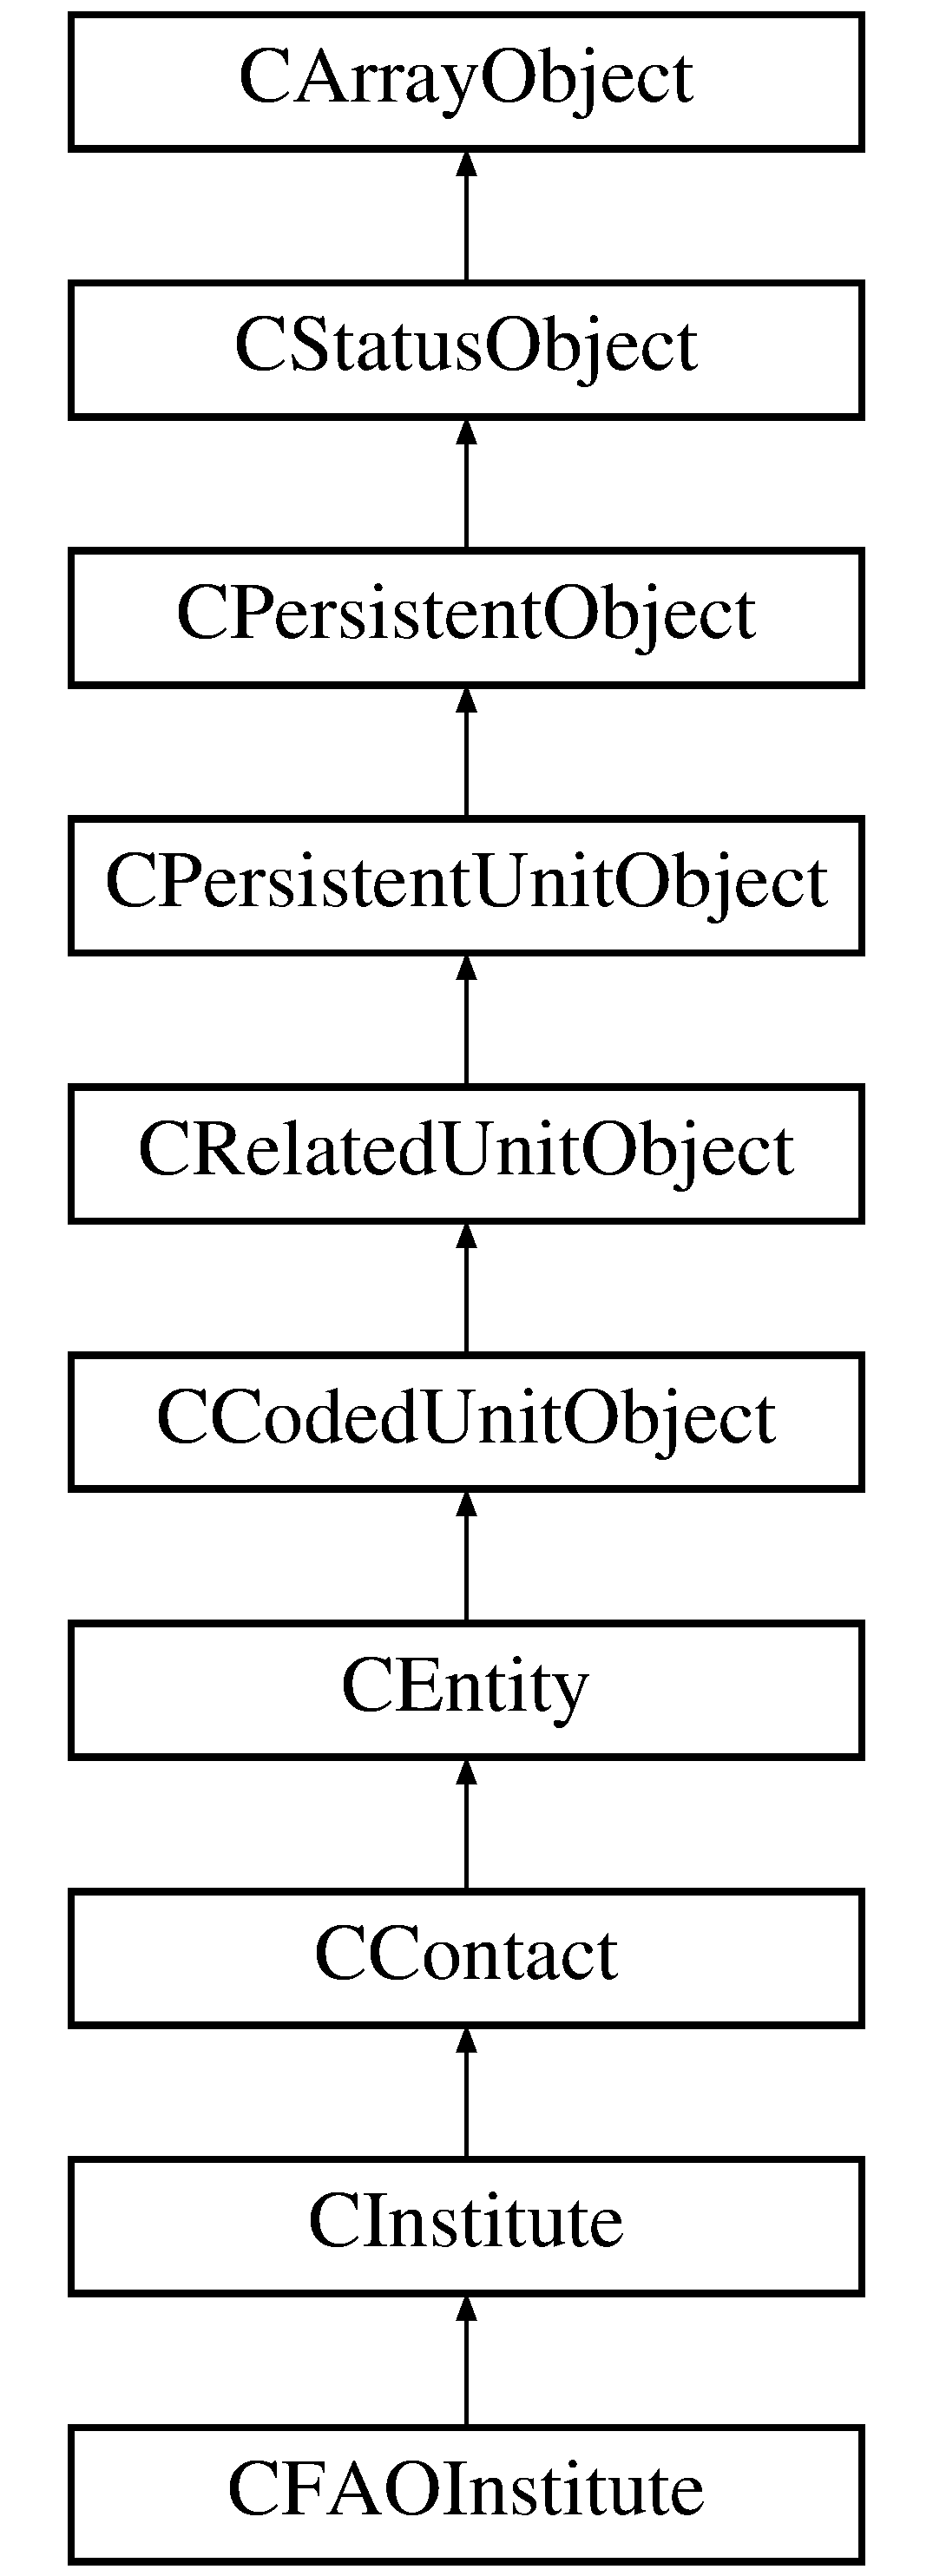
\includegraphics[height=10.000000cm]{class_c_institute}
\end{center}
\end{figure}
\subsection*{Public Member Functions}
\begin{DoxyCompactItemize}
\item 
\hyperlink{class_c_institute_a468ba723fabd5a67bea5016d1531b147}{\-\_\-\-\_\-construct} (\$the\-Container=N\-U\-L\-L, \$the\-Identifier=N\-U\-L\-L, \$the\-Modifiers=k\-F\-L\-A\-G\-\_\-\-D\-E\-F\-A\-U\-L\-T)
\item 
\hyperlink{class_c_institute_a0484d97ec619358927d914932eddb396}{Acronym} (\$the\-Value=N\-U\-L\-L, \$the\-Operation=N\-U\-L\-L, \$get\-Old=F\-A\-L\-S\-E)
\item 
\hyperlink{class_c_institute_af981115a3d7d208e17090f37b328979f}{U\-R\-L} (\$the\-Value=N\-U\-L\-L, \$the\-Type=N\-U\-L\-L, \$get\-Old=F\-A\-L\-S\-E)
\item 
\hyperlink{class_c_institute_a16c349e22775161c89dbf73850b24cd7}{offset\-Set} (\$the\-Offset, \$the\-Value)
\item 
\hyperlink{class_c_institute_a8f82ded3b52a6fb609c67e45669e1454}{offset\-Unset} (\$the\-Offset)
\end{DoxyCompactItemize}
\subsection*{Static Public Member Functions}
\begin{DoxyCompactItemize}
\item 
static \hyperlink{class_c_institute_a7a6915d35bc47272faabe8111574dddc}{Hash\-Index} (\$the\-Value)
\end{DoxyCompactItemize}
\subsection*{Protected Member Functions}
\begin{DoxyCompactItemize}
\item 
\hyperlink{class_c_institute_a096aa38309ae2f88250700d5755a18a6}{\-\_\-\-Prepare\-Commit} (\&\$the\-Container, \&\$the\-Identifier, \&\$the\-Modifiers)
\end{DoxyCompactItemize}
\subsection*{Additional Inherited Members}


\subsection{Constructor \& Destructor Documentation}
\hypertarget{class_c_institute_a468ba723fabd5a67bea5016d1531b147}{\index{C\-Institute@{C\-Institute}!\-\_\-\-\_\-construct@{\-\_\-\-\_\-construct}}
\index{\-\_\-\-\_\-construct@{\-\_\-\-\_\-construct}!CInstitute@{C\-Institute}}
\subsubsection[{\-\_\-\-\_\-construct}]{\setlength{\rightskip}{0pt plus 5cm}C\-Institute\-::\-\_\-\-\_\-construct (
\begin{DoxyParamCaption}
\item[{}]{\$the\-Container = {\ttfamily NULL}, }
\item[{}]{\$the\-Identifier = {\ttfamily NULL}, }
\item[{}]{\$the\-Modifiers = {\ttfamily kFLAG\-\_\-DEFAULT}}
\end{DoxyParamCaption}
)}}\label{class_c_institute_a468ba723fabd5a67bea5016d1531b147}
Instantiate class.

We \hyperlink{class_c_coded_unit_object_a314fc62af62314f5ac5acca2ac809900}{overload} the constructor to initialise the \hyperlink{class_c_status_object_a8429102e4f52f7558649b64f4e673a69}{inited} \hyperlink{}{flag} if the \hyperlink{class_c_entity_ace5878c009baf09d85c8ca115c48dbb0}{name} element is set.

We also enforce the \hyperlink{class_c_persistent_object_aa8dc7db66e2af3d28c2035161a2aabf9}{encoded} \hyperlink{}{flag}.


\begin{DoxyParams}[1]{Parameters}
mixed & {\em \$the\-Container} & Persistent container. \\
\hline
mixed & {\em \$the\-Identifier} & Object identifier. \\
\hline
bitfield & {\em \$the\-Modifiers} & Create modifiers.\\
\hline
\end{DoxyParams}
public 

Reimplemented from \hyperlink{class_c_coded_unit_object_a314fc62af62314f5ac5acca2ac809900}{C\-Coded\-Unit\-Object}.



\subsection{Member Function Documentation}
\hypertarget{class_c_institute_a096aa38309ae2f88250700d5755a18a6}{\index{C\-Institute@{C\-Institute}!\-\_\-\-Prepare\-Commit@{\-\_\-\-Prepare\-Commit}}
\index{\-\_\-\-Prepare\-Commit@{\-\_\-\-Prepare\-Commit}!CInstitute@{C\-Institute}}
\subsubsection[{\-\_\-\-Prepare\-Commit}]{\setlength{\rightskip}{0pt plus 5cm}C\-Institute\-::\-\_\-\-Prepare\-Commit (
\begin{DoxyParamCaption}
\item[{\&}]{\$the\-Container, }
\item[{\&}]{\$the\-Identifier, }
\item[{\&}]{\$the\-Modifiers}
\end{DoxyParamCaption}
)\hspace{0.3cm}{\ttfamily [protected]}}}\label{class_c_institute_a096aa38309ae2f88250700d5755a18a6}
Normalise parameters of a store.

We overload this method to initialise the \hyperlink{}{k\-E\-N\-T\-I\-T\-Y\-\_\-\-I\-N\-S\-T} \hyperlink{}{type} to the object prior \hyperlink{class_c_persistent_object_a88b1f2b11d3d60e0b3d33d8b0649b68a}{saving} it.

We also force the \hyperlink{class_c_persistent_object_aa8dc7db66e2af3d28c2035161a2aabf9}{encoded} \hyperlink{}{flag}.


\begin{DoxyParams}[1]{Parameters}
reference & {\em \&\$the\-Container} & Object container. \\
\hline
reference & {\em \&\$the\-Identifier} & Object identifier. \\
\hline
reference & {\em \&\$the\-Modifiers} & Commit modifiers.\\
\hline
\end{DoxyParams}
protected


\begin{DoxyExceptions}{Exceptions}
{\em \{@link} & \hyperlink{class_c_exception}{C\-Exception} \hyperlink{class_c_exception}{C\-Exception}\}\\
\hline
\end{DoxyExceptions}
\begin{DoxySeeAlso}{See Also}
k\-E\-R\-R\-O\-R\-\_\-\-O\-P\-T\-I\-O\-N\-\_\-\-M\-I\-S\-S\-I\-N\-G 
\end{DoxySeeAlso}


Reimplemented from \hyperlink{class_c_entity_ac306808f0f8404fa405674cbe14fd441}{C\-Entity}.



Reimplemented in \hyperlink{class_c_f_a_o_institute_a9917150b0e31b741aa10c9443e880746}{C\-F\-A\-O\-Institute}.

\hypertarget{class_c_institute_a0484d97ec619358927d914932eddb396}{\index{C\-Institute@{C\-Institute}!Acronym@{Acronym}}
\index{Acronym@{Acronym}!CInstitute@{C\-Institute}}
\subsubsection[{Acronym}]{\setlength{\rightskip}{0pt plus 5cm}C\-Institute\-::\-Acronym (
\begin{DoxyParamCaption}
\item[{}]{\$the\-Value = {\ttfamily NULL}, }
\item[{}]{\$the\-Operation = {\ttfamily NULL}, }
\item[{}]{\$get\-Old = {\ttfamily FALSE}}
\end{DoxyParamCaption}
)}}\label{class_c_institute_a0484d97ec619358927d914932eddb396}
Manage entity acronyms.

This method can be used to handle the institute \hyperlink{}{acronyms} list, it uses the standard accessor \hyperlink{class_c_attribute_ace756c1a8832932ec135104223d1e50c}{method} to manage the list of acronyms.

Each element of this list should indicate an acronym by which one refers to the current institute, the nature and specifics of these elements is the responsibility of concrete classes.

For a more thorough reference of how this method works, please consult the \hyperlink{class_c_attribute_ace756c1a8832932ec135104223d1e50c}{C\-Attribute\-::\-Manage\-Array\-Offset} method, in which the second parameter will be the constant \hyperlink{}{k\-O\-F\-F\-S\-E\-T\-\_\-\-A\-C\-R\-O\-N\-Y\-M}.


\begin{DoxyParams}[1]{Parameters}
mixed & {\em \$the\-Value} & Value or index. \\
\hline
mixed & {\em \$the\-Operation} & Operation. \\
\hline
boolean & {\em \$get\-Old} & T\-R\-U\-E get old value.\\
\hline
\end{DoxyParams}
public \begin{DoxyReturn}{Returns}
mixed
\end{DoxyReturn}
\hyperlink{class_c_attribute_ace756c1a8832932ec135104223d1e50c}{C\-Attribute\-::\-Manage\-Array\-Offset()}

\begin{DoxySeeAlso}{See Also}
k\-O\-F\-F\-S\-E\-T\-\_\-\-A\-C\-R\-O\-N\-Y\-M 
\end{DoxySeeAlso}
\hypertarget{class_c_institute_a7a6915d35bc47272faabe8111574dddc}{\index{C\-Institute@{C\-Institute}!Hash\-Index@{Hash\-Index}}
\index{Hash\-Index@{Hash\-Index}!CInstitute@{C\-Institute}}
\subsubsection[{Hash\-Index}]{\setlength{\rightskip}{0pt plus 5cm}static C\-Institute\-::\-Hash\-Index (
\begin{DoxyParamCaption}
\item[{}]{\$the\-Value}
\end{DoxyParamCaption}
)\hspace{0.3cm}{\ttfamily [static]}}}\label{class_c_institute_a7a6915d35bc47272faabe8111574dddc}
Hash index.

This method can be used to format an identifier provided as a string, it will be used by the \hyperlink{class_c_persistent_unit_object_ad1ca0920cf0df3c24351402f9afbf34b}{\-\_\-id} method to format the result of the \hyperlink{class_c_coded_unit_object_a990c19b8bf98d2784da81e3a3121ce56}{\-\_\-index} method. One can consider this as the index hashing method for all derived classes.

In this class we take the provided \hyperlink{class_c_coded_unit_object_a56af949800e65f9a283239d2e455259f}{code} and prefix it with the \hyperlink{}{k\-E\-N\-T\-I\-T\-Y\-\_\-\-I\-N\-S\-T} token, the result will be \hyperlink{class_c_data_type_binary}{hashed}


\begin{DoxyParams}[1]{Parameters}
string & {\em \$the\-Value} & Value to hash.\\
\hline
\end{DoxyParams}
\begin{DoxyReturn}{Returns}
string 
\end{DoxyReturn}


Reimplemented from \hyperlink{class_c_persistent_unit_object_af0e75c386b883074c8bb677bac500bb3}{C\-Persistent\-Unit\-Object}.



Reimplemented in \hyperlink{class_c_f_a_o_institute_ad9004a3928ad07bdac2988f48c5a8cdd}{C\-F\-A\-O\-Institute}.

\hypertarget{class_c_institute_a16c349e22775161c89dbf73850b24cd7}{\index{C\-Institute@{C\-Institute}!offset\-Set@{offset\-Set}}
\index{offset\-Set@{offset\-Set}!CInstitute@{C\-Institute}}
\subsubsection[{offset\-Set}]{\setlength{\rightskip}{0pt plus 5cm}C\-Institute\-::offset\-Set (
\begin{DoxyParamCaption}
\item[{}]{\$the\-Offset, }
\item[{}]{\$the\-Value}
\end{DoxyParamCaption}
)}}\label{class_c_institute_a16c349e22775161c89dbf73850b24cd7}
Set a value for a given offset.

We overload this method to manage the \hyperlink{class_c_status_object_a8429102e4f52f7558649b64f4e673a69}{inited} \hyperlink{}{status}\-: this is set if the \hyperlink{}{name}, \hyperlink{}{e-\/mail}, \hyperlink{}{password} and the parent \hyperlink{}{code} are set.


\begin{DoxyParams}[1]{Parameters}
string & {\em \$the\-Offset} & Offset. \\
\hline
string | N\-U\-L\-L & {\em \$the\-Value} & Value to set at offset.\\
\hline
\end{DoxyParams}
public

\hyperlink{class_c_status_object_a8429102e4f52f7558649b64f4e673a69}{\-\_\-\-Is\-Inited()}  \hyperlink{class_c_persistent_object_a6520a7bcecf3f39fd61ec6d08f736e77}{\-\_\-\-Is\-Committed()} 

Reimplemented from \hyperlink{class_c_coded_unit_object_a49bb8f2956cb0551ba827b222778f295}{C\-Coded\-Unit\-Object}.



Reimplemented in \hyperlink{class_c_f_a_o_institute_ac819c5bfa381ffa0f78b34442d2ea3c2}{C\-F\-A\-O\-Institute}.

\hypertarget{class_c_institute_a8f82ded3b52a6fb609c67e45669e1454}{\index{C\-Institute@{C\-Institute}!offset\-Unset@{offset\-Unset}}
\index{offset\-Unset@{offset\-Unset}!CInstitute@{C\-Institute}}
\subsubsection[{offset\-Unset}]{\setlength{\rightskip}{0pt plus 5cm}C\-Institute\-::offset\-Unset (
\begin{DoxyParamCaption}
\item[{}]{\$the\-Offset}
\end{DoxyParamCaption}
)}}\label{class_c_institute_a8f82ded3b52a6fb609c67e45669e1454}
Reset a value for a given offset.

We overload this method to manage the \hyperlink{class_c_status_object_a8429102e4f52f7558649b64f4e673a69}{inited} \hyperlink{}{status}\-: this is set if the \hyperlink{}{name}, \hyperlink{}{e-\/mail}, \hyperlink{}{password} and the parent \hyperlink{}{code} are set.


\begin{DoxyParams}[1]{Parameters}
string & {\em \$the\-Offset} & Offset.\\
\hline
\end{DoxyParams}
public

\hyperlink{class_c_status_object_a8429102e4f52f7558649b64f4e673a69}{\-\_\-\-Is\-Inited()}  \hyperlink{class_c_persistent_object_a6520a7bcecf3f39fd61ec6d08f736e77}{\-\_\-\-Is\-Committed()} 

Reimplemented from \hyperlink{class_c_coded_unit_object_a5072e0f72c19260df212a4cf93c9f1cb}{C\-Coded\-Unit\-Object}.



Reimplemented in \hyperlink{class_c_f_a_o_institute_a3bd7c59a3da53ba8c3cd1d9d0ff5ae0a}{C\-F\-A\-O\-Institute}.

\hypertarget{class_c_institute_af981115a3d7d208e17090f37b328979f}{\index{C\-Institute@{C\-Institute}!U\-R\-L@{U\-R\-L}}
\index{U\-R\-L@{U\-R\-L}!CInstitute@{C\-Institute}}
\subsubsection[{U\-R\-L}]{\setlength{\rightskip}{0pt plus 5cm}C\-Institute\-::\-U\-R\-L (
\begin{DoxyParamCaption}
\item[{}]{\$the\-Value = {\ttfamily NULL}, }
\item[{}]{\$the\-Type = {\ttfamily NULL}, }
\item[{}]{\$get\-Old = {\ttfamily FALSE}}
\end{DoxyParamCaption}
)}}\label{class_c_institute_af981115a3d7d208e17090f37b328979f}
Manage institute urls.

This method can be used to manage the institute \hyperlink{}{U\-R\-L} or web pages list, the method expects the following parameters\-:


\begin{DoxyItemize}
\item {\bfseries \$the\-Value}\-: The value or operation\-: 
\begin{DoxyItemize}
\item {\itshape N\-U\-L\-L}\-: Return the current value selected by the second parameter. 
\item {\itshape F\-A\-L\-S\-E}\-: Delete the value selected by the second parameter. 
\item {\itshape other}\-: Set value selected by the second parameter. 
\end{DoxyItemize}
\item {\bfseries \$the\-Type}\-: The element type, kind or index\-: 
\begin{DoxyItemize}
\item {\itshape N\-U\-L\-L}\-: This value indicates that the U\-R\-L has no type or kind, in general, when adding elements, this case applies to default elements. 
\item {\itshape other}\-: All other types will be interpreted as the kind or type of the U\-R\-L. 
\end{DoxyItemize}
\item {\bfseries \$get\-Old}\-: Determines what the method will return\-: 
\begin{DoxyItemize}
\item {\itshape T\-R\-U\-E}\-: Return the value {\itshape before} it was eventually modified. 
\item {\itshape F\-A\-L\-S\-E}\-: Return the value {\itshape after} it was eventually modified. 
\end{DoxyItemize}
\end{DoxyItemize}


\begin{DoxyParams}[1]{Parameters}
string & {\em \$the\-Value} & U\-R\-L or operation. \\
\hline
mixed & {\em \$the\-Type} & Mailing address kind or index. \\
\hline
boolean & {\em \$get\-Old} & T\-R\-U\-E get old value.\\
\hline
\end{DoxyParams}
public \begin{DoxyReturn}{Returns}
string 
\end{DoxyReturn}


The documentation for this class was generated from the following file\-:\begin{DoxyCompactItemize}
\item 
/\-Library/\-Web\-Server/\-Library/wrapper/classes/C\-Institute.\-php\end{DoxyCompactItemize}

\hypertarget{class_c_mail_address}{\section{C\-Mail\-Address Class Reference}
\label{class_c_mail_address}\index{C\-Mail\-Address@{C\-Mail\-Address}}
}
Inheritance diagram for C\-Mail\-Address\-:\begin{figure}[H]
\begin{center}
\leavevmode
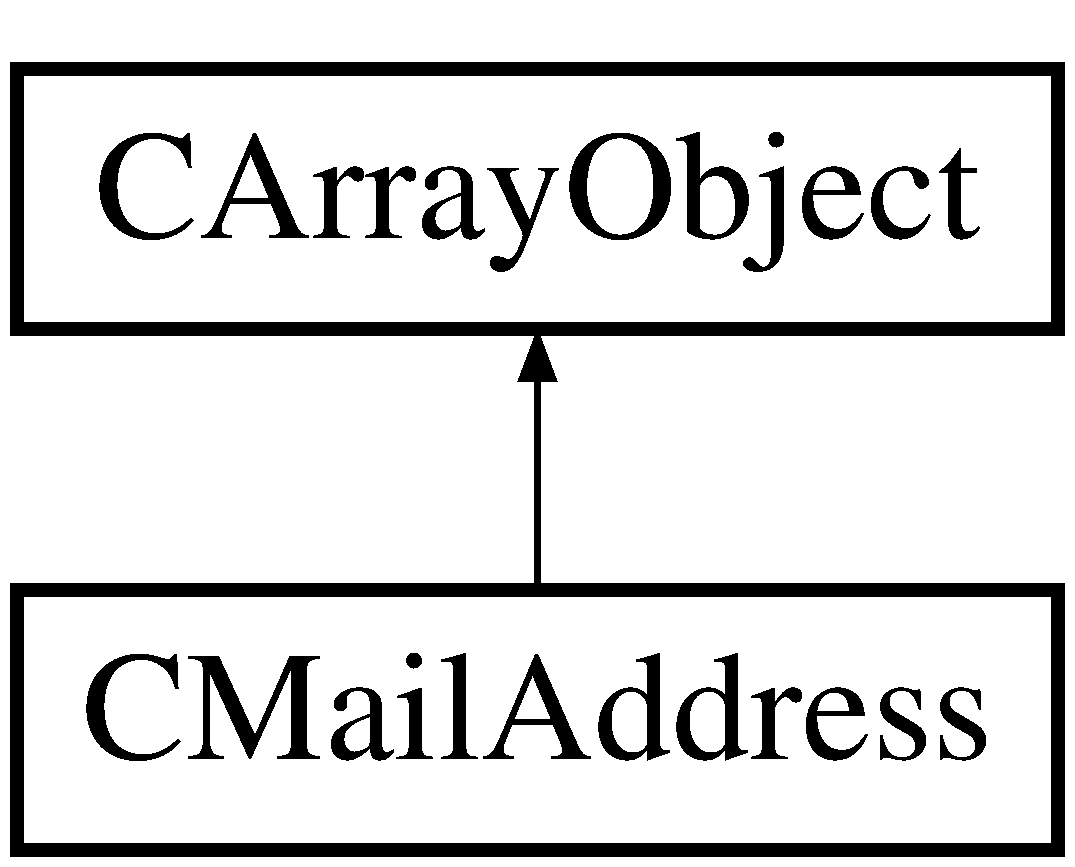
\includegraphics[height=2.000000cm]{class_c_mail_address}
\end{center}
\end{figure}
\subsection*{Public Member Functions}
\begin{DoxyCompactItemize}
\item 
\hyperlink{class_c_mail_address_a6c1a89dabb933fe8cc82c7579d91b764}{\-\_\-\-\_\-construct} (\$the\-Address=N\-U\-L\-L)
\item 
\hyperlink{class_c_mail_address_a84de4b41187ae62787e661f5c7fd750e}{Place} (\$the\-Value=N\-U\-L\-L, \$get\-Old=F\-A\-L\-S\-E)
\item 
\hyperlink{class_c_mail_address_a607c00bd7b2dc17c986e1bdf0d821a6a}{Care} (\$the\-Value=N\-U\-L\-L, \$get\-Old=F\-A\-L\-S\-E)
\item 
\hyperlink{class_c_mail_address_a4e0c4fbb0ff61bc678f18f8cab421f44}{Street} (\$the\-Value=N\-U\-L\-L, \$get\-Old=F\-A\-L\-S\-E)
\item 
\hyperlink{class_c_mail_address_a00b413b11f642c386d4389a54725e963}{Zip} (\$the\-Value=N\-U\-L\-L, \$get\-Old=F\-A\-L\-S\-E)
\item 
\hyperlink{class_c_mail_address_a38cea06af29000931b0e05e1cbef375c}{City} (\$the\-Value=N\-U\-L\-L, \$get\-Old=F\-A\-L\-S\-E)
\item 
\hyperlink{class_c_mail_address_a931ae6ed594d5eadf4a7390ed06426c5}{Province} (\$the\-Value=N\-U\-L\-L, \$get\-Old=F\-A\-L\-S\-E)
\item 
\hyperlink{class_c_mail_address_a1abebf29998a4c1bc04d32f2f7059da6}{Country} (\$the\-Value=N\-U\-L\-L, \$get\-Old=F\-A\-L\-S\-E)
\item 
\hyperlink{class_c_mail_address_a660d959c10bd32b1454615d0c804d93e}{Full} (\$the\-Value=N\-U\-L\-L, \$get\-Old=F\-A\-L\-S\-E)
\end{DoxyCompactItemize}


\subsection{Constructor \& Destructor Documentation}
\hypertarget{class_c_mail_address_a6c1a89dabb933fe8cc82c7579d91b764}{\index{C\-Mail\-Address@{C\-Mail\-Address}!\-\_\-\-\_\-construct@{\-\_\-\-\_\-construct}}
\index{\-\_\-\-\_\-construct@{\-\_\-\-\_\-construct}!CMailAddress@{C\-Mail\-Address}}
\subsubsection[{\-\_\-\-\_\-construct}]{\setlength{\rightskip}{0pt plus 5cm}C\-Mail\-Address\-::\-\_\-\-\_\-construct (
\begin{DoxyParamCaption}
\item[{}]{\$the\-Address = {\ttfamily NULL}}
\end{DoxyParamCaption}
)}}\label{class_c_mail_address_a6c1a89dabb933fe8cc82c7579d91b764}
Instantiate class.

The constructor will instantiate an object either from an array, by loading all corresponding properties, from a string, in which case it will be interpreted as the \hyperlink{class_c_mail_address_a660d959c10bd32b1454615d0c804d93e}{full} address, or as an empty address.


\begin{DoxyParams}[1]{Parameters}
mixed & {\em \$the\-Address} & Address structure or string.\\
\hline
\end{DoxyParams}
public 

\subsection{Member Function Documentation}
\hypertarget{class_c_mail_address_a607c00bd7b2dc17c986e1bdf0d821a6a}{\index{C\-Mail\-Address@{C\-Mail\-Address}!Care@{Care}}
\index{Care@{Care}!CMailAddress@{C\-Mail\-Address}}
\subsubsection[{Care}]{\setlength{\rightskip}{0pt plus 5cm}C\-Mail\-Address\-::\-Care (
\begin{DoxyParamCaption}
\item[{}]{\$the\-Value = {\ttfamily NULL}, }
\item[{}]{\$get\-Old = {\ttfamily FALSE}}
\end{DoxyParamCaption}
)}}\label{class_c_mail_address_a607c00bd7b2dc17c986e1bdf0d821a6a}
Manage care-\/of.

This method can be used to manage the address \hyperlink{}{care-\/of}, it accepts a parameter which represents a care-\/of reference or the requested operation, depending on its value\-:


\begin{DoxyItemize}
\item {\itshape N\-U\-L\-L}\-: Return the current value. 
\item {\itshape F\-A\-L\-S\-E}\-: Delete the current value. 
\item {\itshape other}\-: Set the value with the provided parameter. 
\end{DoxyItemize}

The second parameter is a boolean which if {\itshape T\-R\-U\-E} will return the {\itshape old} value when replacing values; if {\itshape F\-A\-L\-S\-E}, it will return the currently set value.


\begin{DoxyParams}[1]{Parameters}
string & {\em \$the\-Value} & Value or operation. \\
\hline
boolean & {\em \$get\-Old} & T\-R\-U\-E get old value.\\
\hline
\end{DoxyParams}
public \begin{DoxyReturn}{Returns}
mixed
\end{DoxyReturn}
\hyperlink{class_c_attribute_a9d231a47718719fcd6c33f3d0ac91675}{C\-Attribute\-::\-Manage\-Offset()}

\begin{DoxySeeAlso}{See also}
k\-O\-F\-F\-S\-E\-T\-\_\-\-C\-A\-R\-E 
\end{DoxySeeAlso}
\hypertarget{class_c_mail_address_a38cea06af29000931b0e05e1cbef375c}{\index{C\-Mail\-Address@{C\-Mail\-Address}!City@{City}}
\index{City@{City}!CMailAddress@{C\-Mail\-Address}}
\subsubsection[{City}]{\setlength{\rightskip}{0pt plus 5cm}C\-Mail\-Address\-::\-City (
\begin{DoxyParamCaption}
\item[{}]{\$the\-Value = {\ttfamily NULL}, }
\item[{}]{\$get\-Old = {\ttfamily FALSE}}
\end{DoxyParamCaption}
)}}\label{class_c_mail_address_a38cea06af29000931b0e05e1cbef375c}
Manage city.

This method can be used to manage the address \hyperlink{}{city}, it accepts a parameter which represents the address city name or the requested operation, depending on its value\-:


\begin{DoxyItemize}
\item {\itshape N\-U\-L\-L}\-: Return the current value. 
\item {\itshape F\-A\-L\-S\-E}\-: Delete the current value. 
\item {\itshape other}\-: Set the value with the provided parameter. 
\end{DoxyItemize}

The second parameter is a boolean which if {\itshape T\-R\-U\-E} will return the {\itshape old} value when replacing values; if {\itshape F\-A\-L\-S\-E}, it will return the currently set value.


\begin{DoxyParams}[1]{Parameters}
string & {\em \$the\-Value} & Value or operation. \\
\hline
boolean & {\em \$get\-Old} & T\-R\-U\-E get old value.\\
\hline
\end{DoxyParams}
public \begin{DoxyReturn}{Returns}
mixed
\end{DoxyReturn}
\hyperlink{class_c_attribute_a9d231a47718719fcd6c33f3d0ac91675}{C\-Attribute\-::\-Manage\-Offset()}

\begin{DoxySeeAlso}{See also}
k\-O\-F\-F\-S\-E\-T\-\_\-\-C\-I\-T\-Y 
\end{DoxySeeAlso}
\hypertarget{class_c_mail_address_a1abebf29998a4c1bc04d32f2f7059da6}{\index{C\-Mail\-Address@{C\-Mail\-Address}!Country@{Country}}
\index{Country@{Country}!CMailAddress@{C\-Mail\-Address}}
\subsubsection[{Country}]{\setlength{\rightskip}{0pt plus 5cm}C\-Mail\-Address\-::\-Country (
\begin{DoxyParamCaption}
\item[{}]{\$the\-Value = {\ttfamily NULL}, }
\item[{}]{\$get\-Old = {\ttfamily FALSE}}
\end{DoxyParamCaption}
)}}\label{class_c_mail_address_a1abebf29998a4c1bc04d32f2f7059da6}
Manage province.

This method can be used to manage the address \hyperlink{}{country}, it accepts a parameter which represents the address country name, code or the requested operation, depending on its value\-:


\begin{DoxyItemize}
\item {\itshape N\-U\-L\-L}\-: Return the current value. 
\item {\itshape F\-A\-L\-S\-E}\-: Delete the current value. 
\item {\itshape other}\-: Set the value with the provided parameter. 
\end{DoxyItemize}

The second parameter is a boolean which if {\itshape T\-R\-U\-E} will return the {\itshape old} value when replacing values; if {\itshape F\-A\-L\-S\-E}, it will return the currently set value.


\begin{DoxyParams}[1]{Parameters}
string & {\em \$the\-Value} & Value or operation. \\
\hline
boolean & {\em \$get\-Old} & T\-R\-U\-E get old value.\\
\hline
\end{DoxyParams}
public \begin{DoxyReturn}{Returns}
mixed
\end{DoxyReturn}
\hyperlink{class_c_attribute_a9d231a47718719fcd6c33f3d0ac91675}{C\-Attribute\-::\-Manage\-Offset()}

\begin{DoxySeeAlso}{See also}
k\-O\-F\-F\-S\-E\-T\-\_\-\-C\-O\-U\-N\-T\-R\-Y 
\end{DoxySeeAlso}
\hypertarget{class_c_mail_address_a660d959c10bd32b1454615d0c804d93e}{\index{C\-Mail\-Address@{C\-Mail\-Address}!Full@{Full}}
\index{Full@{Full}!CMailAddress@{C\-Mail\-Address}}
\subsubsection[{Full}]{\setlength{\rightskip}{0pt plus 5cm}C\-Mail\-Address\-::\-Full (
\begin{DoxyParamCaption}
\item[{}]{\$the\-Value = {\ttfamily NULL}, }
\item[{}]{\$get\-Old = {\ttfamily FALSE}}
\end{DoxyParamCaption}
)}}\label{class_c_mail_address_a660d959c10bd32b1454615d0c804d93e}
Manage full address.

This method can be used to manage the full address as a \hyperlink{}{string}, it accepts a parameter which represents the full address or the requested operation, depending on its value\-:


\begin{DoxyItemize}
\item {\itshape N\-U\-L\-L}\-: Return the current value. 
\item {\itshape F\-A\-L\-S\-E}\-: Delete the current value. 
\item {\itshape other}\-: Set the value with the provided parameter. 
\end{DoxyItemize}

The second parameter is a boolean which if {\itshape T\-R\-U\-E} will return the {\itshape old} value when replacing values; if {\itshape F\-A\-L\-S\-E}, it will return the currently set value.

When retrieving values, if the full address was not set, this method will return in any case the string representation of the full address.


\begin{DoxyParams}[1]{Parameters}
string & {\em \$the\-Value} & Value or operation. \\
\hline
boolean & {\em \$get\-Old} & T\-R\-U\-E get old value.\\
\hline
\end{DoxyParams}
public \begin{DoxyReturn}{Returns}
mixed
\end{DoxyReturn}
\hyperlink{class_c_attribute_a9d231a47718719fcd6c33f3d0ac91675}{C\-Attribute\-::\-Manage\-Offset()}

\begin{DoxySeeAlso}{See also}
k\-O\-F\-F\-S\-E\-T\-\_\-\-F\-U\-L\-L 
\end{DoxySeeAlso}
\hypertarget{class_c_mail_address_a84de4b41187ae62787e661f5c7fd750e}{\index{C\-Mail\-Address@{C\-Mail\-Address}!Place@{Place}}
\index{Place@{Place}!CMailAddress@{C\-Mail\-Address}}
\subsubsection[{Place}]{\setlength{\rightskip}{0pt plus 5cm}C\-Mail\-Address\-::\-Place (
\begin{DoxyParamCaption}
\item[{}]{\$the\-Value = {\ttfamily NULL}, }
\item[{}]{\$get\-Old = {\ttfamily FALSE}}
\end{DoxyParamCaption}
)}}\label{class_c_mail_address_a84de4b41187ae62787e661f5c7fd750e}
Manage place.

This method can be used to manage the address \hyperlink{}{place}, it accepts a parameter which represents either the place name or the requested operation, depending on its value\-:


\begin{DoxyItemize}
\item {\itshape N\-U\-L\-L}\-: Return the current value. 
\item {\itshape F\-A\-L\-S\-E}\-: Delete the current value. 
\item {\itshape other}\-: Set the value with the provided parameter. 
\end{DoxyItemize}

The second parameter is a boolean which if {\itshape T\-R\-U\-E} will return the {\itshape old} value when replacing values; if {\itshape F\-A\-L\-S\-E}, it will return the currently set value.


\begin{DoxyParams}[1]{Parameters}
string & {\em \$the\-Value} & Value or operation. \\
\hline
boolean & {\em \$get\-Old} & T\-R\-U\-E get old value.\\
\hline
\end{DoxyParams}
public \begin{DoxyReturn}{Returns}
mixed
\end{DoxyReturn}
\hyperlink{class_c_attribute_a9d231a47718719fcd6c33f3d0ac91675}{C\-Attribute\-::\-Manage\-Offset()}

\begin{DoxySeeAlso}{See also}
k\-O\-F\-F\-S\-E\-T\-\_\-\-P\-L\-A\-C\-E 
\end{DoxySeeAlso}
\hypertarget{class_c_mail_address_a931ae6ed594d5eadf4a7390ed06426c5}{\index{C\-Mail\-Address@{C\-Mail\-Address}!Province@{Province}}
\index{Province@{Province}!CMailAddress@{C\-Mail\-Address}}
\subsubsection[{Province}]{\setlength{\rightskip}{0pt plus 5cm}C\-Mail\-Address\-::\-Province (
\begin{DoxyParamCaption}
\item[{}]{\$the\-Value = {\ttfamily NULL}, }
\item[{}]{\$get\-Old = {\ttfamily FALSE}}
\end{DoxyParamCaption}
)}}\label{class_c_mail_address_a931ae6ed594d5eadf4a7390ed06426c5}
Manage province.

This method can be used to manage the address \hyperlink{}{province}, it accepts a parameter which represents the address province name, code or the requested operation, depending on its value\-:


\begin{DoxyItemize}
\item {\itshape N\-U\-L\-L}\-: Return the current value. 
\item {\itshape F\-A\-L\-S\-E}\-: Delete the current value. 
\item {\itshape other}\-: Set the value with the provided parameter. 
\end{DoxyItemize}

The second parameter is a boolean which if {\itshape T\-R\-U\-E} will return the {\itshape old} value when replacing values; if {\itshape F\-A\-L\-S\-E}, it will return the currently set value.


\begin{DoxyParams}[1]{Parameters}
string & {\em \$the\-Value} & Value or operation. \\
\hline
boolean & {\em \$get\-Old} & T\-R\-U\-E get old value.\\
\hline
\end{DoxyParams}
public \begin{DoxyReturn}{Returns}
mixed
\end{DoxyReturn}
\hyperlink{class_c_attribute_a9d231a47718719fcd6c33f3d0ac91675}{C\-Attribute\-::\-Manage\-Offset()}

\begin{DoxySeeAlso}{See also}
k\-O\-F\-F\-S\-E\-T\-\_\-\-P\-R\-O\-V\-I\-N\-C\-E 
\end{DoxySeeAlso}
\hypertarget{class_c_mail_address_a4e0c4fbb0ff61bc678f18f8cab421f44}{\index{C\-Mail\-Address@{C\-Mail\-Address}!Street@{Street}}
\index{Street@{Street}!CMailAddress@{C\-Mail\-Address}}
\subsubsection[{Street}]{\setlength{\rightskip}{0pt plus 5cm}C\-Mail\-Address\-::\-Street (
\begin{DoxyParamCaption}
\item[{}]{\$the\-Value = {\ttfamily NULL}, }
\item[{}]{\$get\-Old = {\ttfamily FALSE}}
\end{DoxyParamCaption}
)}}\label{class_c_mail_address_a4e0c4fbb0ff61bc678f18f8cab421f44}
Manage street.

This method can be used to manage the address \hyperlink{}{street}, it accepts a parameter which represents a street name, P.\-O. box or the requested operation, depending on its value\-:


\begin{DoxyItemize}
\item {\itshape N\-U\-L\-L}\-: Return the current value. 
\item {\itshape F\-A\-L\-S\-E}\-: Delete the current value. 
\item {\itshape other}\-: Set the value with the provided parameter. 
\end{DoxyItemize}

The second parameter is a boolean which if {\itshape T\-R\-U\-E} will return the {\itshape old} value when replacing values; if {\itshape F\-A\-L\-S\-E}, it will return the currently set value.


\begin{DoxyParams}[1]{Parameters}
string & {\em \$the\-Value} & Value or operation. \\
\hline
boolean & {\em \$get\-Old} & T\-R\-U\-E get old value.\\
\hline
\end{DoxyParams}
public \begin{DoxyReturn}{Returns}
mixed
\end{DoxyReturn}
\hyperlink{class_c_attribute_a9d231a47718719fcd6c33f3d0ac91675}{C\-Attribute\-::\-Manage\-Offset()}

\begin{DoxySeeAlso}{See also}
k\-O\-F\-F\-S\-E\-T\-\_\-\-S\-T\-R\-E\-E\-T 
\end{DoxySeeAlso}
\hypertarget{class_c_mail_address_a00b413b11f642c386d4389a54725e963}{\index{C\-Mail\-Address@{C\-Mail\-Address}!Zip@{Zip}}
\index{Zip@{Zip}!CMailAddress@{C\-Mail\-Address}}
\subsubsection[{Zip}]{\setlength{\rightskip}{0pt plus 5cm}C\-Mail\-Address\-::\-Zip (
\begin{DoxyParamCaption}
\item[{}]{\$the\-Value = {\ttfamily NULL}, }
\item[{}]{\$get\-Old = {\ttfamily FALSE}}
\end{DoxyParamCaption}
)}}\label{class_c_mail_address_a00b413b11f642c386d4389a54725e963}
Manage zip code.

This method can be used to manage the address \hyperlink{}{zip} code, it accepts a parameter which represents the address zip code or the requested operation, depending on its value\-:


\begin{DoxyItemize}
\item {\itshape N\-U\-L\-L}\-: Return the current value. 
\item {\itshape F\-A\-L\-S\-E}\-: Delete the current value. 
\item {\itshape other}\-: Set the value with the provided parameter. 
\end{DoxyItemize}

The second parameter is a boolean which if {\itshape T\-R\-U\-E} will return the {\itshape old} value when replacing values; if {\itshape F\-A\-L\-S\-E}, it will return the currently set value.


\begin{DoxyParams}[1]{Parameters}
string & {\em \$the\-Value} & Value or operation. \\
\hline
boolean & {\em \$get\-Old} & T\-R\-U\-E get old value.\\
\hline
\end{DoxyParams}
public \begin{DoxyReturn}{Returns}
mixed
\end{DoxyReturn}
\hyperlink{class_c_attribute_a9d231a47718719fcd6c33f3d0ac91675}{C\-Attribute\-::\-Manage\-Offset()}

\begin{DoxySeeAlso}{See also}
k\-O\-F\-F\-S\-E\-T\-\_\-\-Z\-I\-P\-\_\-\-C\-O\-D\-E 
\end{DoxySeeAlso}


The documentation for this class was generated from the following file\-:\begin{DoxyCompactItemize}
\item 
/\-Library/\-Web\-Server/\-Library/wrapper/classes/C\-Mail\-Address.\-php\end{DoxyCompactItemize}

\hypertarget{class_c_mongo_container}{\section{C\-Mongo\-Container Class Reference}
\label{class_c_mongo_container}\index{C\-Mongo\-Container@{C\-Mongo\-Container}}
}
Inheritance diagram for C\-Mongo\-Container\-:\begin{figure}[H]
\begin{center}
\leavevmode
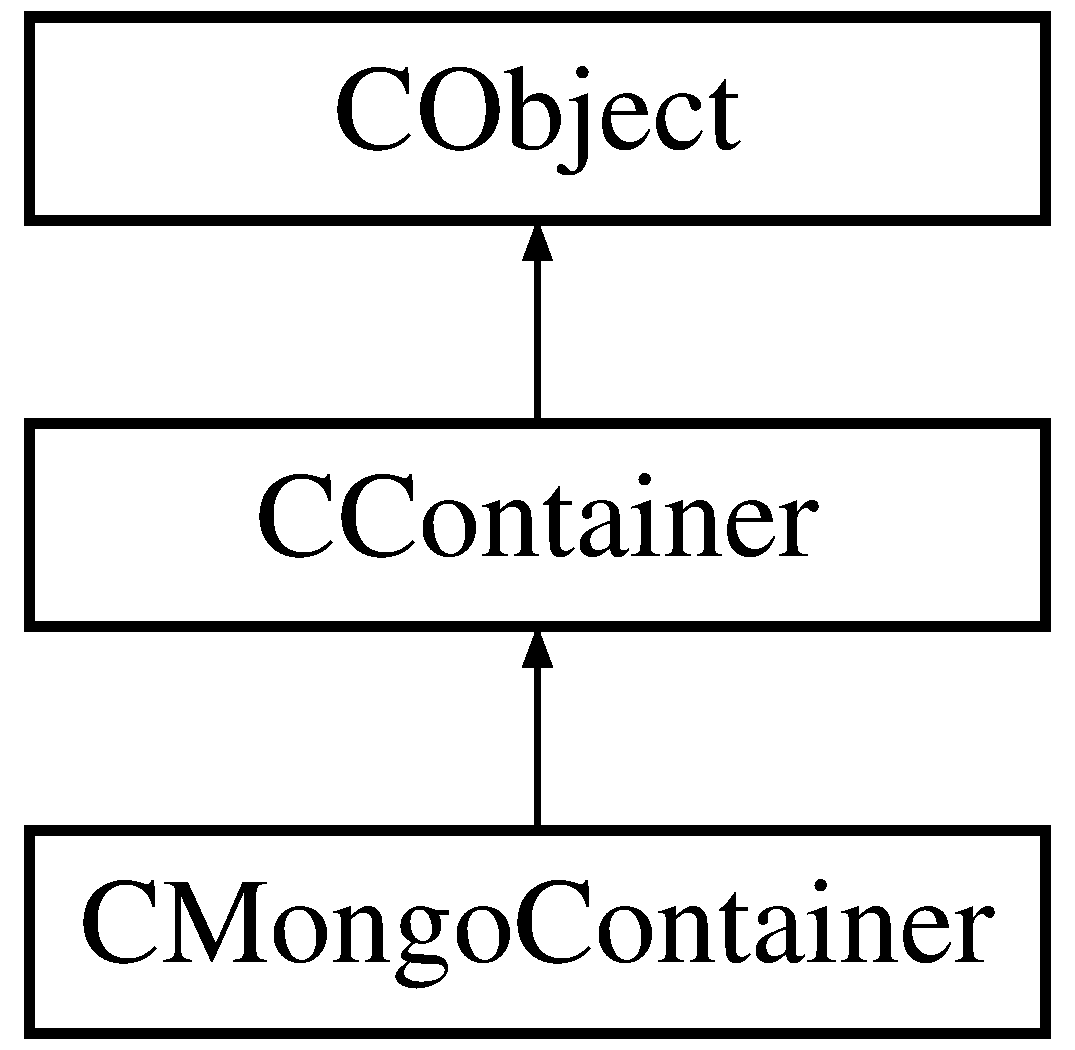
\includegraphics[height=4.000000cm]{class_c_mongo_container}
\end{center}
\end{figure}
\subsection*{Public Member Functions}
\begin{DoxyCompactItemize}
\item 
\hyperlink{class_c_mongo_container_abc325eae251667da577efdb45a7d3c17}{\-\_\-\-\_\-to\-String} ()
\item 
\hyperlink{class_c_mongo_container_a253978bb8e4d1e2613665d308de83e1e}{Container} (\$the\-Value=N\-U\-L\-L, \$get\-Old=F\-A\-L\-S\-E)
\item 
\hyperlink{class_c_mongo_container_a27a99b6ea891b226729bc6cb8426cac0}{Database} ()
\item 
\hyperlink{class_c_mongo_container_a077bdbf148dfa01f3798015906e4e70a}{Unserialise\-Data} (\&\$the\-Element)
\end{DoxyCompactItemize}
\subsection*{Protected Member Functions}
\begin{DoxyCompactItemize}
\item 
\hyperlink{class_c_mongo_container_a92cbcdba4f2b0bda2ae3eeb7a08d7ba2}{\-\_\-\-Commit} (\&\$the\-Object, \&\$the\-Identifier, \&\$the\-Modifiers)
\item 
\hyperlink{class_c_mongo_container_a61f469d1975834b22665392542620317}{\-\_\-\-Load} (\&\$the\-Identifier, \&\$the\-Modifiers)
\item 
\hyperlink{class_c_mongo_container_aa516a049efe0c9083e2f8c5b9f9076a4}{\-\_\-\-Delete} (\&\$the\-Identifier, \&\$the\-Modifiers)
\item 
\hyperlink{class_c_mongo_container_af592e4500a640190f374c18683af3b83}{\-\_\-\-Prepare\-Commit} (\&\$the\-Object, \&\$the\-Identifier, \&\$the\-Modifiers)
\item 
\hyperlink{class_c_mongo_container_a2c44e9229169abde420adf34045f5382}{\-\_\-\-Prepare\-Load} (\&\$the\-Identifier, \&\$the\-Modifiers)
\end{DoxyCompactItemize}
\subsection*{Additional Inherited Members}


\subsection{Member Function Documentation}
\hypertarget{class_c_mongo_container_abc325eae251667da577efdb45a7d3c17}{\index{C\-Mongo\-Container@{C\-Mongo\-Container}!\-\_\-\-\_\-to\-String@{\-\_\-\-\_\-to\-String}}
\index{\-\_\-\-\_\-to\-String@{\-\_\-\-\_\-to\-String}!CMongoContainer@{C\-Mongo\-Container}}
\subsubsection[{\-\_\-\-\_\-to\-String}]{\setlength{\rightskip}{0pt plus 5cm}C\-Mongo\-Container\-::\-\_\-\-\_\-to\-String (
\begin{DoxyParamCaption}
{}
\end{DoxyParamCaption}
)}}\label{class_c_mongo_container_abc325eae251667da577efdb45a7d3c17}
Return container name.

This method should return the current container's name.

In this class we return the collection name.

public \begin{DoxyReturn}{Returns}
string
\end{DoxyReturn}
\hyperlink{class_c_mongo_container_a253978bb8e4d1e2613665d308de83e1e}{Container()} 

Reimplemented from \hyperlink{class_c_container_aa1d6ed5052f55cdffcf6445968f203ed}{C\-Container}.

\hypertarget{class_c_mongo_container_a92cbcdba4f2b0bda2ae3eeb7a08d7ba2}{\index{C\-Mongo\-Container@{C\-Mongo\-Container}!\-\_\-\-Commit@{\-\_\-\-Commit}}
\index{\-\_\-\-Commit@{\-\_\-\-Commit}!CMongoContainer@{C\-Mongo\-Container}}
\subsubsection[{\-\_\-\-Commit}]{\setlength{\rightskip}{0pt plus 5cm}C\-Mongo\-Container\-::\-\_\-\-Commit (
\begin{DoxyParamCaption}
\item[{\&}]{\$the\-Object, }
\item[{\&}]{\$the\-Identifier, }
\item[{\&}]{\$the\-Modifiers}
\end{DoxyParamCaption}
)\hspace{0.3cm}{\ttfamily [protected]}}}\label{class_c_mongo_container_a92cbcdba4f2b0bda2ae3eeb7a08d7ba2}
Commit provided object.

We implement this method to handle Mongo\-Collection object stores, this method will store the object in the current container.

The method will check if the current container is a Mongo\-Collection, if this is not the case, it will raise an \hyperlink{}{exception}.

If the provided modifiers indicate a \hyperlink{}{modify} operation, the method will return the modified object, in all other cases the method will return the object identifier.


\begin{DoxyParams}[1]{Parameters}
reference & {\em \&\$the\-Object} & Object to commit. \\
\hline
reference & {\em \&\$the\-Identifier} & Object identifier. \\
\hline
reference & {\em \&\$the\-Modifiers} & Commit modifiers.\\
\hline
\end{DoxyParams}
protected \begin{DoxyReturn}{Returns}
mixed
\end{DoxyReturn}
\hyperlink{class_c_mongo_container_a253978bb8e4d1e2613665d308de83e1e}{Container()}

\begin{DoxySeeAlso}{See Also}
k\-F\-L\-A\-G\-\_\-\-P\-E\-R\-S\-I\-S\-T\-\_\-\-I\-N\-S\-E\-R\-T k\-F\-L\-A\-G\-\_\-\-P\-E\-R\-S\-I\-S\-T\-\_\-\-M\-O\-D\-I\-F\-Y 

k\-F\-L\-A\-G\-\_\-\-P\-E\-R\-S\-I\-S\-T\-\_\-\-R\-E\-P\-L\-A\-C\-E k\-F\-L\-A\-G\-\_\-\-P\-E\-R\-S\-I\-S\-T\-\_\-\-U\-P\-D\-A\-T\-E 
\end{DoxySeeAlso}


Reimplemented from \hyperlink{class_c_container_acbc85dd164615b31c9edfec93bcf27f9}{C\-Container}.



Reimplemented in \hyperlink{class_c_mongo_grid_container_a1dc8378e77df7c06afc2c733e2422482}{C\-Mongo\-Grid\-Container}.

\hypertarget{class_c_mongo_container_aa516a049efe0c9083e2f8c5b9f9076a4}{\index{C\-Mongo\-Container@{C\-Mongo\-Container}!\-\_\-\-Delete@{\-\_\-\-Delete}}
\index{\-\_\-\-Delete@{\-\_\-\-Delete}!CMongoContainer@{C\-Mongo\-Container}}
\subsubsection[{\-\_\-\-Delete}]{\setlength{\rightskip}{0pt plus 5cm}C\-Mongo\-Container\-::\-\_\-\-Delete (
\begin{DoxyParamCaption}
\item[{\&}]{\$the\-Identifier, }
\item[{\&}]{\$the\-Modifiers}
\end{DoxyParamCaption}
)\hspace{0.3cm}{\ttfamily [protected]}}}\label{class_c_mongo_container_aa516a049efe0c9083e2f8c5b9f9076a4}
Delete object.

We implement this method to handle Mongo\-Collection object stores, this method will remove the object from the current container.


\begin{DoxyParams}[1]{Parameters}
reference & {\em \&\$the\-Identifier} & Object identifier. \\
\hline
reference & {\em \&\$the\-Modifiers} & Load modifiers.\\
\hline
\end{DoxyParams}
protected \begin{DoxyReturn}{Returns}
mixed 
\end{DoxyReturn}


Reimplemented from \hyperlink{class_c_container_a20aac3eec154c2122f2c602bf5ce35fe}{C\-Container}.

\hypertarget{class_c_mongo_container_a61f469d1975834b22665392542620317}{\index{C\-Mongo\-Container@{C\-Mongo\-Container}!\-\_\-\-Load@{\-\_\-\-Load}}
\index{\-\_\-\-Load@{\-\_\-\-Load}!CMongoContainer@{C\-Mongo\-Container}}
\subsubsection[{\-\_\-\-Load}]{\setlength{\rightskip}{0pt plus 5cm}C\-Mongo\-Container\-::\-\_\-\-Load (
\begin{DoxyParamCaption}
\item[{\&}]{\$the\-Identifier, }
\item[{\&}]{\$the\-Modifiers}
\end{DoxyParamCaption}
)\hspace{0.3cm}{\ttfamily [protected]}}}\label{class_c_mongo_container_a61f469d1975834b22665392542620317}
Load object.

We implement this method to handle Mongo\-Collection object stores, this method will retrieve the object from the current container.

The \hyperlink{class_c_container_a48db96aa6bbf15d0bfc15725616b7154}{caller} will have resolved references andeventually extracted the identifier from the provided parameter.

If the provided parameter is an array, the method will assume it is a query; if not, the method will assume it is the value to match against the \hyperlink{}{local} identifier.

The method will use the {\itshape find\-One} method to retrieve the object.


\begin{DoxyParams}[1]{Parameters}
reference & {\em \&\$the\-Identifier} & Object identifier. \\
\hline
reference & {\em \&\$the\-Modifiers} & Load modifiers.\\
\hline
\end{DoxyParams}
protected \begin{DoxyReturn}{Returns}
mixed 
\end{DoxyReturn}


Reimplemented from \hyperlink{class_c_container_a865f140560991fa21a88b7fc8ff8f1f5}{C\-Container}.

\hypertarget{class_c_mongo_container_af592e4500a640190f374c18683af3b83}{\index{C\-Mongo\-Container@{C\-Mongo\-Container}!\-\_\-\-Prepare\-Commit@{\-\_\-\-Prepare\-Commit}}
\index{\-\_\-\-Prepare\-Commit@{\-\_\-\-Prepare\-Commit}!CMongoContainer@{C\-Mongo\-Container}}
\subsubsection[{\-\_\-\-Prepare\-Commit}]{\setlength{\rightskip}{0pt plus 5cm}C\-Mongo\-Container\-::\-\_\-\-Prepare\-Commit (
\begin{DoxyParamCaption}
\item[{\&}]{\$the\-Object, }
\item[{\&}]{\$the\-Identifier, }
\item[{\&}]{\$the\-Modifiers}
\end{DoxyParamCaption}
)\hspace{0.3cm}{\ttfamily [protected]}}}\label{class_c_mongo_container_af592e4500a640190f374c18683af3b83}
Prepare before a \hyperlink{class_c_mongo_container_a92cbcdba4f2b0bda2ae3eeb7a08d7ba2}{commit}.

We \hyperlink{class_c_container_a0dc47e54abc533cedf1c2c0f915d96b2}{overload} this method to handle the identifier\-: if provided, it means that that is to become the object's unique \hyperlink{}{identifier}; if not provided and the object has an \hyperlink{}{identifier}, we use that one.

We also raise an exception if the provided object is not either an array or an Array\-Object.


\begin{DoxyParams}[1]{Parameters}
reference & {\em \&\$the\-Object} & Object or data. \\
\hline
reference & {\em \&\$the\-Identifier} & Object identifier. \\
\hline
reference & {\em \&\$the\-Modifiers} & Commit modifiers.\\
\hline
\end{DoxyParams}
protected


\begin{DoxyExceptions}{Exceptions}
{\em \{@link} & \hyperlink{class_c_exception}{C\-Exception} \hyperlink{class_c_exception}{C\-Exception}\}\\
\hline
\end{DoxyExceptions}
\hyperlink{class_c_mongo_container_a253978bb8e4d1e2613665d308de83e1e}{Container()}

\begin{DoxySeeAlso}{See Also}
k\-F\-L\-A\-G\-\_\-\-S\-T\-A\-T\-E\-\_\-\-E\-N\-C\-O\-D\-E\-D 

k\-E\-R\-R\-O\-R\-\_\-\-O\-P\-T\-I\-O\-N\-\_\-\-M\-I\-S\-S\-I\-N\-G k\-E\-R\-R\-O\-R\-\_\-\-I\-N\-V\-A\-L\-I\-D\-\_\-\-P\-A\-R\-A\-M\-E\-T\-E\-R k\-E\-R\-R\-O\-R\-\_\-\-I\-N\-V\-A\-L\-I\-D\-\_\-\-S\-T\-A\-T\-E 
\end{DoxySeeAlso}


Reimplemented from \hyperlink{class_c_container_a0dc47e54abc533cedf1c2c0f915d96b2}{C\-Container}.



Reimplemented in \hyperlink{class_c_mongo_grid_container_a94715c26002c38020a8e4103d3075426}{C\-Mongo\-Grid\-Container}.

\hypertarget{class_c_mongo_container_a2c44e9229169abde420adf34045f5382}{\index{C\-Mongo\-Container@{C\-Mongo\-Container}!\-\_\-\-Prepare\-Load@{\-\_\-\-Prepare\-Load}}
\index{\-\_\-\-Prepare\-Load@{\-\_\-\-Prepare\-Load}!CMongoContainer@{C\-Mongo\-Container}}
\subsubsection[{\-\_\-\-Prepare\-Load}]{\setlength{\rightskip}{0pt plus 5cm}C\-Mongo\-Container\-::\-\_\-\-Prepare\-Load (
\begin{DoxyParamCaption}
\item[{\&}]{\$the\-Identifier, }
\item[{\&}]{\$the\-Modifiers}
\end{DoxyParamCaption}
)\hspace{0.3cm}{\ttfamily [protected]}}}\label{class_c_mongo_container_a2c44e9229169abde420adf34045f5382}
Prepare before a \hyperlink{class_c_mongo_container_a61f469d1975834b22665392542620317}{load}.

The duty of this method is to ensure that the parameters provided to the \hyperlink{class_c_mongo_container_a61f469d1975834b22665392542620317}{find} operation are valid.

In this class we \hyperlink{class_c_container_a1b84868c32fcfd3e11a9f6cc85fc461c}{overload} this method to handle identifiers provided as queries.


\begin{DoxyParams}[1]{Parameters}
reference & {\em \&\$the\-Identifier} & Object identifier. \\
\hline
reference & {\em \&\$the\-Modifiers} & Create modifiers.\\
\hline
\end{DoxyParams}
protected


\begin{DoxyExceptions}{Exceptions}
{\em \{@link} & \hyperlink{class_c_exception}{C\-Exception} \hyperlink{class_c_exception}{C\-Exception}\}\\
\hline
\end{DoxyExceptions}
\hyperlink{class_c_mongo_container_a253978bb8e4d1e2613665d308de83e1e}{Container()}  \hyperlink{class_c_mongo_container_a077bdbf148dfa01f3798015906e4e70a}{Unserialise\-Data()}

\begin{DoxySeeAlso}{See Also}
k\-F\-L\-A\-G\-\_\-\-S\-T\-A\-T\-E\-\_\-\-E\-N\-C\-O\-D\-E\-D 
\end{DoxySeeAlso}


Reimplemented from \hyperlink{class_c_container_a1b84868c32fcfd3e11a9f6cc85fc461c}{C\-Container}.

\hypertarget{class_c_mongo_container_a253978bb8e4d1e2613665d308de83e1e}{\index{C\-Mongo\-Container@{C\-Mongo\-Container}!Container@{Container}}
\index{Container@{Container}!CMongoContainer@{C\-Mongo\-Container}}
\subsubsection[{Container}]{\setlength{\rightskip}{0pt plus 5cm}C\-Mongo\-Container\-::\-Container (
\begin{DoxyParamCaption}
\item[{}]{\$the\-Value = {\ttfamily NULL}, }
\item[{}]{\$get\-Old = {\ttfamily FALSE}}
\end{DoxyParamCaption}
)}}\label{class_c_mongo_container_a253978bb8e4d1e2613665d308de83e1e}
Manage persistent container.

We \hyperlink{class_c_container_a7d10fa70dfa381cb95e66c265e2ca113}{overload} this method to ensure that the provided container is a Mongo\-Collection object.


\begin{DoxyParams}[1]{Parameters}
mixed & {\em \$the\-Value} & Persistent container or operation. \\
\hline
boolean & {\em \$get\-Old} & T\-R\-U\-E get old value.\\
\hline
\end{DoxyParams}
public \begin{DoxyReturn}{Returns}
mixed 
\end{DoxyReturn}


Reimplemented from \hyperlink{class_c_container_a7d10fa70dfa381cb95e66c265e2ca113}{C\-Container}.



Reimplemented in \hyperlink{class_c_mongo_grid_container_aafde59c8f7bf042d0e4f3a8d7bc87d90}{C\-Mongo\-Grid\-Container}.

\hypertarget{class_c_mongo_container_a27a99b6ea891b226729bc6cb8426cac0}{\index{C\-Mongo\-Container@{C\-Mongo\-Container}!Database@{Database}}
\index{Database@{Database}!CMongoContainer@{C\-Mongo\-Container}}
\subsubsection[{Database}]{\setlength{\rightskip}{0pt plus 5cm}C\-Mongo\-Container\-::\-Database (
\begin{DoxyParamCaption}
{}
\end{DoxyParamCaption}
)}}\label{class_c_mongo_container_a27a99b6ea891b226729bc6cb8426cac0}
Return database.

In this class we return the collection's database.

public \begin{DoxyReturn}{Returns}
mixed
\end{DoxyReturn}
\hyperlink{class_c_mongo_container_a253978bb8e4d1e2613665d308de83e1e}{Container()} 

Reimplemented from \hyperlink{class_c_container_a0d691b62d9b70b924e24a332931ce9d1}{C\-Container}.

\hypertarget{class_c_mongo_container_a077bdbf148dfa01f3798015906e4e70a}{\index{C\-Mongo\-Container@{C\-Mongo\-Container}!Unserialise\-Data@{Unserialise\-Data}}
\index{Unserialise\-Data@{Unserialise\-Data}!CMongoContainer@{C\-Mongo\-Container}}
\subsubsection[{Unserialise\-Data}]{\setlength{\rightskip}{0pt plus 5cm}C\-Mongo\-Container\-::\-Unserialise\-Data (
\begin{DoxyParamCaption}
\item[{\&}]{\$the\-Element}
\end{DoxyParamCaption}
)}}\label{class_c_mongo_container_a077bdbf148dfa01f3798015906e4e70a}
Unserialise provided data element.

We \hyperlink{class_c_container_a09d585e2a9809221a42d52d7520c9cbf}{implement} this method to convert all standard \hyperlink{class_c_data_type}{types} into custom Mongo data types.

In this class we parse the following types and \hyperlink{}{offsets}\-:


\begin{DoxyItemize}
\item {\itshape \hyperlink{class_c_data_type_mongo_id}{C\-Data\-Type\-Mongo\-Id} object or \hyperlink{}{k\-T\-Y\-P\-E\-\_\-\-Mongo\-Id} offset}\-: We return a Mongo\-Id object. 
\item {\itshape \hyperlink{class_c_data_type_mongo_code}{C\-Data\-Type\-Mongo\-Code} object or \hyperlink{}{k\-T\-Y\-P\-E\-\_\-\-Mongo\-Code} offset}\-: We return a Mongo\-Code object. 
\item {\itshape \hyperlink{class_c_data_type_stamp}{C\-Data\-Type\-Stamp} object or \hyperlink{}{k\-T\-Y\-P\-E\-\_\-\-S\-T\-A\-M\-P} offset}\-: We return a Mongo\-Date object. 
\item {\itshape \hyperlink{class_c_data_type_regex}{C\-Data\-Type\-Regex} object or \hyperlink{}{k\-T\-Y\-P\-E\-\_\-\-R\-E\-G\-E\-X} offset}\-: We return a Mongo\-Regex object. 
\item {\itshape \hyperlink{class_c_data_type_int32}{C\-Data\-Type\-Int32} object or \hyperlink{}{k\-T\-Y\-P\-E\-\_\-\-I\-N\-T32} offset}\-: We return a Mongo\-Int32 object. 
\item {\itshape \hyperlink{class_c_data_type_int64}{C\-Data\-Type\-Int64} object or \hyperlink{}{k\-T\-Y\-P\-E\-\_\-\-I\-N\-T64} offset}\-: We return a Mongo\-Int64 object. 
\item {\itshape \hyperlink{class_c_data_type_binary}{C\-Data\-Type\-Binary} object or \hyperlink{}{k\-T\-Y\-P\-E\-\_\-\-B\-I\-N\-A\-R\-Y} offset}\-: We return a Mongo\-Bin\-Data object. 
\end{DoxyItemize}


\begin{DoxyParams}[1]{Parameters}
reference & {\em \&\$the\-Element} & Element to encode.\\
\hline
\end{DoxyParams}
public 

Reimplemented from \hyperlink{class_c_container_a09d585e2a9809221a42d52d7520c9cbf}{C\-Container}.



The documentation for this class was generated from the following file\-:\begin{DoxyCompactItemize}
\item 
/\-Library/\-Web\-Server/\-Library/wrapper/classes/C\-Mongo\-Container.\-php\end{DoxyCompactItemize}

\hypertarget{class_c_mongo_data_wrapper}{\section{C\-Mongo\-Data\-Wrapper Class Reference}
\label{class_c_mongo_data_wrapper}\index{C\-Mongo\-Data\-Wrapper@{C\-Mongo\-Data\-Wrapper}}
}
Inheritance diagram for C\-Mongo\-Data\-Wrapper\-:\begin{figure}[H]
\begin{center}
\leavevmode
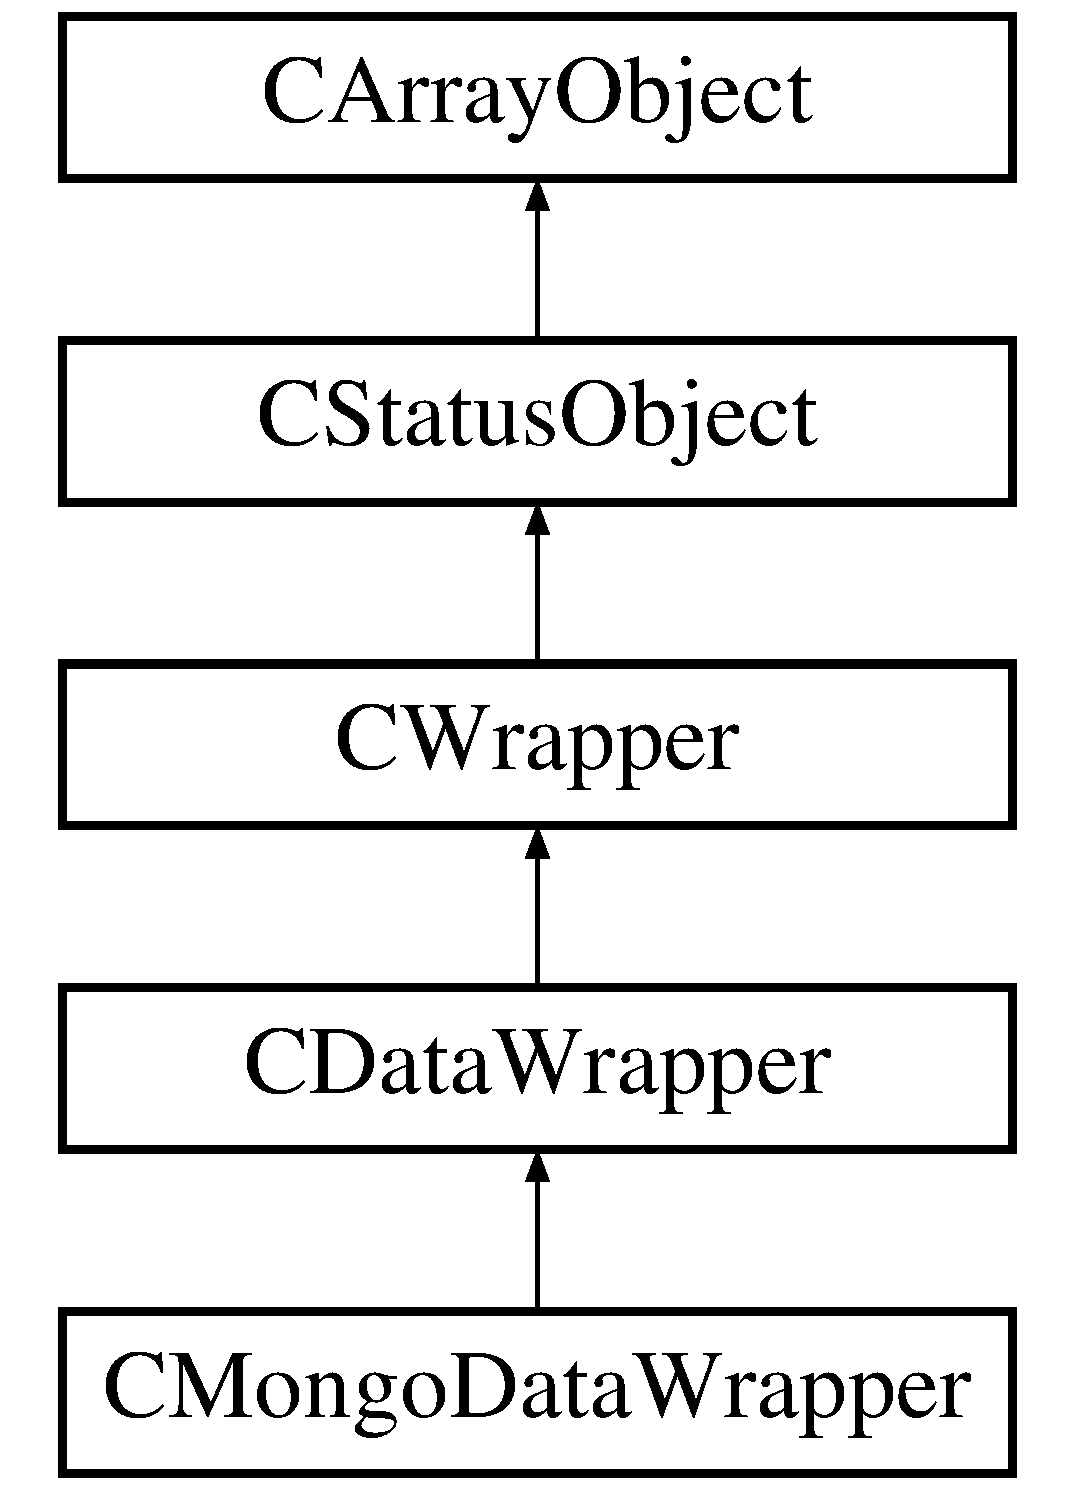
\includegraphics[height=6.000000cm]{class_c_mongo_data_wrapper}
\end{center}
\end{figure}
\subsection*{Protected Member Functions}
\begin{DoxyCompactItemize}
\item 
\hyperlink{class_c_mongo_data_wrapper_a33ff97c26b97d00a67f97d41f67ce47b}{\-\_\-\-Init\-Resources} ()
\item 
\hyperlink{class_c_mongo_data_wrapper_a8ac2f23cfc78f3fba6b256718ed2d105}{\-\_\-\-Parse\-Request} ()
\item 
\hyperlink{class_c_mongo_data_wrapper_abbc0d41394dda4a27eefa8481065749a}{\-\_\-\-Format\-Request} ()
\item 
\hyperlink{class_c_mongo_data_wrapper_a3d06376cb588e5c26751bff3f0083ef5}{\-\_\-\-Validate\-Request} ()
\item 
\hyperlink{class_c_mongo_data_wrapper_adb77016dd91f53f6e5d74a7390020c4d}{\-\_\-\-Parse\-No\-Response} ()
\item 
\hyperlink{class_c_mongo_data_wrapper_a15b44586fe5de968efb0edbe96f3da60}{\-\_\-\-Format\-Database} ()
\item 
\hyperlink{class_c_mongo_data_wrapper_a117d32ff4a01a54a7ff6203ba0ca66b7}{\-\_\-\-Format\-Container} ()
\item 
\hyperlink{class_c_mongo_data_wrapper_a807db77c3c4f7708e86873a0447b83ff}{\-\_\-\-Format\-Query} ()
\item 
\hyperlink{class_c_mongo_data_wrapper_a2642638da121e471c7ea1fbb61f6f3ef}{\-\_\-\-Format\-Object} ()
\item 
\hyperlink{class_c_mongo_data_wrapper_a406b81115b5f3957e6d40ee49ae85a13}{\-\_\-\-Validate\-Operation} ()
\item 
\hyperlink{class_c_mongo_data_wrapper_a9bb974219920f005b1cdba39793b84d5}{\-\_\-\-Validate\-Object} ()
\item 
\hyperlink{class_c_mongo_data_wrapper_aa2ae2292a247d94c9b1dfa13d9a4fb85}{\-\_\-\-Validate\-Query} ()
\item 
\hyperlink{class_c_mongo_data_wrapper_a811af7e7574a459bc56afa3afa99e1a8}{\-\_\-\-Handle\-Request} ()
\item 
\hyperlink{class_c_mongo_data_wrapper_a1ca51f95510a94bf26e004ef2e8e8d37}{\-\_\-\-Handle\-\_\-\-List\-Op} (\&\$the\-List)
\item 
\hyperlink{class_c_mongo_data_wrapper_a226970d3cfb96f8e85e46d3943c25089}{\-\_\-\-Handle\-\_\-\-Get\-Object\-By\-Reference} ()
\item 
\hyperlink{class_c_mongo_data_wrapper_ae7cc52809c8b6cea94c84d5f64a4308b}{\-\_\-\-Handle\-\_\-\-Count} ()
\item 
\hyperlink{class_c_mongo_data_wrapper_a3b9896d121c899aa3dd9f5e56e44c874}{\-\_\-\-Handle\-\_\-\-Get\-One} ()
\item 
\hyperlink{class_c_mongo_data_wrapper_a157a45bd4a2da43bd05d62b22faf3dc6}{\-\_\-\-Handle\-\_\-\-Get} ()
\item 
\hyperlink{class_c_mongo_data_wrapper_a8b9654ce201a453a76a5075bd7ce8a38}{\-\_\-\-Handle\-\_\-\-Match} ()
\item 
\hyperlink{class_c_mongo_data_wrapper_a3b59e4f2efbe64568c500756a170af29}{\-\_\-\-Handle\-\_\-\-Set} ()
\item 
\hyperlink{class_c_mongo_data_wrapper_adc1ef56d8c5fe9dbab74a821f38fe62c}{\-\_\-\-Handle\-\_\-\-Insert} ()
\item 
\hyperlink{class_c_mongo_data_wrapper_a5618d7ca3fe124a76bb62360525b01be}{\-\_\-\-Handle\-\_\-\-Batch\-Insert} ()
\item 
\hyperlink{class_c_mongo_data_wrapper_a271b356a503ae0ab4a67610f808a6a9a}{\-\_\-\-Handle\-\_\-\-Update} ()
\item 
\hyperlink{class_c_mongo_data_wrapper_a1b61fb28b8917a53948b02194902eb34}{\-\_\-\-Handle\-\_\-\-Modify} ()
\item 
\hyperlink{class_c_mongo_data_wrapper_aaed227073838fb79b344e3d07a3152e8}{\-\_\-\-Handle\-\_\-\-Delete} ()
\item 
\hyperlink{class_c_mongo_data_wrapper_ac154306e6919de8316ddf45fc8d619f3}{\-\_\-\-Handle\-Options} (\&\$the\-Result, \$the\-Options)
\end{DoxyCompactItemize}


\subsection{Member Function Documentation}
\hypertarget{class_c_mongo_data_wrapper_a117d32ff4a01a54a7ff6203ba0ca66b7}{\index{C\-Mongo\-Data\-Wrapper@{C\-Mongo\-Data\-Wrapper}!\-\_\-\-Format\-Container@{\-\_\-\-Format\-Container}}
\index{\-\_\-\-Format\-Container@{\-\_\-\-Format\-Container}!CMongoDataWrapper@{C\-Mongo\-Data\-Wrapper}}
\subsubsection[{\-\_\-\-Format\-Container}]{\setlength{\rightskip}{0pt plus 5cm}C\-Mongo\-Data\-Wrapper\-::\-\_\-\-Format\-Container (
\begin{DoxyParamCaption}
{}
\end{DoxyParamCaption}
)\hspace{0.3cm}{\ttfamily [protected]}}}\label{class_c_mongo_data_wrapper_a117d32ff4a01a54a7ff6203ba0ca66b7}
Format container.

This method will format the request container.

In this class we set the request container to a Mongo\-Collection object.

protected \hypertarget{class_c_mongo_data_wrapper_a15b44586fe5de968efb0edbe96f3da60}{\index{C\-Mongo\-Data\-Wrapper@{C\-Mongo\-Data\-Wrapper}!\-\_\-\-Format\-Database@{\-\_\-\-Format\-Database}}
\index{\-\_\-\-Format\-Database@{\-\_\-\-Format\-Database}!CMongoDataWrapper@{C\-Mongo\-Data\-Wrapper}}
\subsubsection[{\-\_\-\-Format\-Database}]{\setlength{\rightskip}{0pt plus 5cm}C\-Mongo\-Data\-Wrapper\-::\-\_\-\-Format\-Database (
\begin{DoxyParamCaption}
{}
\end{DoxyParamCaption}
)\hspace{0.3cm}{\ttfamily [protected]}}}\label{class_c_mongo_data_wrapper_a15b44586fe5de968efb0edbe96f3da60}
Format database.

This method will format the request database.

In this class we set the database to a Mongo\-D\-B object.

protected \hypertarget{class_c_mongo_data_wrapper_a2642638da121e471c7ea1fbb61f6f3ef}{\index{C\-Mongo\-Data\-Wrapper@{C\-Mongo\-Data\-Wrapper}!\-\_\-\-Format\-Object@{\-\_\-\-Format\-Object}}
\index{\-\_\-\-Format\-Object@{\-\_\-\-Format\-Object}!CMongoDataWrapper@{C\-Mongo\-Data\-Wrapper}}
\subsubsection[{\-\_\-\-Format\-Object}]{\setlength{\rightskip}{0pt plus 5cm}C\-Mongo\-Data\-Wrapper\-::\-\_\-\-Format\-Object (
\begin{DoxyParamCaption}
{}
\end{DoxyParamCaption}
)\hspace{0.3cm}{\ttfamily [protected]}}}\label{class_c_mongo_data_wrapper_a2642638da121e471c7ea1fbb61f6f3ef}
Format object.

This method will format the request object.

In this class we resolve the Mongo native types.

protected 

Reimplemented from \hyperlink{class_c_data_wrapper_addefb7bd419de62bfebedc21abbdad7e}{C\-Data\-Wrapper}.

\hypertarget{class_c_mongo_data_wrapper_a807db77c3c4f7708e86873a0447b83ff}{\index{C\-Mongo\-Data\-Wrapper@{C\-Mongo\-Data\-Wrapper}!\-\_\-\-Format\-Query@{\-\_\-\-Format\-Query}}
\index{\-\_\-\-Format\-Query@{\-\_\-\-Format\-Query}!CMongoDataWrapper@{C\-Mongo\-Data\-Wrapper}}
\subsubsection[{\-\_\-\-Format\-Query}]{\setlength{\rightskip}{0pt plus 5cm}C\-Mongo\-Data\-Wrapper\-::\-\_\-\-Format\-Query (
\begin{DoxyParamCaption}
{}
\end{DoxyParamCaption}
)\hspace{0.3cm}{\ttfamily [protected]}}}\label{class_c_mongo_data_wrapper_a807db77c3c4f7708e86873a0447b83ff}
Format query.

This method will format the request query.

In this class we set the query to a \hyperlink{class_c_mongo_query}{C\-Mongo\-Query} object.

protected 

Reimplemented from \hyperlink{class_c_data_wrapper_a0c3054fcf3716d638922cd581d5c706e}{C\-Data\-Wrapper}.

\hypertarget{class_c_mongo_data_wrapper_abbc0d41394dda4a27eefa8481065749a}{\index{C\-Mongo\-Data\-Wrapper@{C\-Mongo\-Data\-Wrapper}!\-\_\-\-Format\-Request@{\-\_\-\-Format\-Request}}
\index{\-\_\-\-Format\-Request@{\-\_\-\-Format\-Request}!CMongoDataWrapper@{C\-Mongo\-Data\-Wrapper}}
\subsubsection[{\-\_\-\-Format\-Request}]{\setlength{\rightskip}{0pt plus 5cm}C\-Mongo\-Data\-Wrapper\-::\-\_\-\-Format\-Request (
\begin{DoxyParamCaption}
{}
\end{DoxyParamCaption}
)\hspace{0.3cm}{\ttfamily [protected]}}}\label{class_c_mongo_data_wrapper_abbc0d41394dda4a27eefa8481065749a}
Format request.

This method should perform any needed formatting before the request will be handled.

In this class we handle the parameters to be decoded

protected 

Reimplemented from \hyperlink{class_c_data_wrapper_ab46c0e9797e8636ca1c9d535b377b90a}{C\-Data\-Wrapper}.



Reimplemented in \hyperlink{class_c_warehouse_wrapper_a4bd0282949f52ce148b60218c48ddde5}{C\-Warehouse\-Wrapper}.

\hypertarget{class_c_mongo_data_wrapper_a5618d7ca3fe124a76bb62360525b01be}{\index{C\-Mongo\-Data\-Wrapper@{C\-Mongo\-Data\-Wrapper}!\-\_\-\-Handle\-\_\-\-Batch\-Insert@{\-\_\-\-Handle\-\_\-\-Batch\-Insert}}
\index{\-\_\-\-Handle\-\_\-\-Batch\-Insert@{\-\_\-\-Handle\-\_\-\-Batch\-Insert}!CMongoDataWrapper@{C\-Mongo\-Data\-Wrapper}}
\subsubsection[{\-\_\-\-Handle\-\_\-\-Batch\-Insert}]{\setlength{\rightskip}{0pt plus 5cm}C\-Mongo\-Data\-Wrapper\-::\-\_\-\-Handle\-\_\-\-Batch\-Insert (
\begin{DoxyParamCaption}
{}
\end{DoxyParamCaption}
)\hspace{0.3cm}{\ttfamily [protected]}}}\label{class_c_mongo_data_wrapper_a5618d7ca3fe124a76bb62360525b01be}
Handle \hyperlink{}{batch} Insert request.

This method will handle the \hyperlink{}{k\-A\-P\-I\-\_\-\-O\-P\-\_\-\-B\-A\-T\-C\-H\-\_\-\-I\-N\-S\-E\-R\-T} request, which will insert the provided list of objects.

protected \hypertarget{class_c_mongo_data_wrapper_ae7cc52809c8b6cea94c84d5f64a4308b}{\index{C\-Mongo\-Data\-Wrapper@{C\-Mongo\-Data\-Wrapper}!\-\_\-\-Handle\-\_\-\-Count@{\-\_\-\-Handle\-\_\-\-Count}}
\index{\-\_\-\-Handle\-\_\-\-Count@{\-\_\-\-Handle\-\_\-\-Count}!CMongoDataWrapper@{C\-Mongo\-Data\-Wrapper}}
\subsubsection[{\-\_\-\-Handle\-\_\-\-Count}]{\setlength{\rightskip}{0pt plus 5cm}C\-Mongo\-Data\-Wrapper\-::\-\_\-\-Handle\-\_\-\-Count (
\begin{DoxyParamCaption}
{}
\end{DoxyParamCaption}
)\hspace{0.3cm}{\ttfamily [protected]}}}\label{class_c_mongo_data_wrapper_ae7cc52809c8b6cea94c84d5f64a4308b}
Handle \hyperlink{}{C\-O\-U\-N\-T} request.

This method will handle the \hyperlink{}{k\-A\-P\-I\-\_\-\-O\-P\-\_\-\-C\-O\-U\-N\-T} request, which returns the total count of a Mongo query.

protected \hypertarget{class_c_mongo_data_wrapper_aaed227073838fb79b344e3d07a3152e8}{\index{C\-Mongo\-Data\-Wrapper@{C\-Mongo\-Data\-Wrapper}!\-\_\-\-Handle\-\_\-\-Delete@{\-\_\-\-Handle\-\_\-\-Delete}}
\index{\-\_\-\-Handle\-\_\-\-Delete@{\-\_\-\-Handle\-\_\-\-Delete}!CMongoDataWrapper@{C\-Mongo\-Data\-Wrapper}}
\subsubsection[{\-\_\-\-Handle\-\_\-\-Delete}]{\setlength{\rightskip}{0pt plus 5cm}C\-Mongo\-Data\-Wrapper\-::\-\_\-\-Handle\-\_\-\-Delete (
\begin{DoxyParamCaption}
{}
\end{DoxyParamCaption}
)\hspace{0.3cm}{\ttfamily [protected]}}}\label{class_c_mongo_data_wrapper_aaed227073838fb79b344e3d07a3152e8}
Handle \hyperlink{}{Delete} request.

This method will handle the \hyperlink{}{k\-A\-P\-I\-\_\-\-O\-P\-\_\-\-D\-E\-L} request, whichwill delete all objects matching the provided filter.

The method expects the {\itshape just\-One} parameter in the provided \hyperlink{}{options}, if not provided, it will default to {\itshape F\-A\-L\-S\-E}.

protected \hypertarget{class_c_mongo_data_wrapper_a157a45bd4a2da43bd05d62b22faf3dc6}{\index{C\-Mongo\-Data\-Wrapper@{C\-Mongo\-Data\-Wrapper}!\-\_\-\-Handle\-\_\-\-Get@{\-\_\-\-Handle\-\_\-\-Get}}
\index{\-\_\-\-Handle\-\_\-\-Get@{\-\_\-\-Handle\-\_\-\-Get}!CMongoDataWrapper@{C\-Mongo\-Data\-Wrapper}}
\subsubsection[{\-\_\-\-Handle\-\_\-\-Get}]{\setlength{\rightskip}{0pt plus 5cm}C\-Mongo\-Data\-Wrapper\-::\-\_\-\-Handle\-\_\-\-Get (
\begin{DoxyParamCaption}
{}
\end{DoxyParamCaption}
)\hspace{0.3cm}{\ttfamily [protected]}}}\label{class_c_mongo_data_wrapper_a157a45bd4a2da43bd05d62b22faf3dc6}
Handle \hyperlink{}{Get} request.

This method will handle the \hyperlink{}{k\-A\-P\-I\-\_\-\-O\-P\-\_\-\-G\-E\-T} request, which corresponds to the find Mongo query.

protected \hypertarget{class_c_mongo_data_wrapper_a226970d3cfb96f8e85e46d3943c25089}{\index{C\-Mongo\-Data\-Wrapper@{C\-Mongo\-Data\-Wrapper}!\-\_\-\-Handle\-\_\-\-Get\-Object\-By\-Reference@{\-\_\-\-Handle\-\_\-\-Get\-Object\-By\-Reference}}
\index{\-\_\-\-Handle\-\_\-\-Get\-Object\-By\-Reference@{\-\_\-\-Handle\-\_\-\-Get\-Object\-By\-Reference}!CMongoDataWrapper@{C\-Mongo\-Data\-Wrapper}}
\subsubsection[{\-\_\-\-Handle\-\_\-\-Get\-Object\-By\-Reference}]{\setlength{\rightskip}{0pt plus 5cm}C\-Mongo\-Data\-Wrapper\-::\-\_\-\-Handle\-\_\-\-Get\-Object\-By\-Reference (
\begin{DoxyParamCaption}
{}
\end{DoxyParamCaption}
)\hspace{0.3cm}{\ttfamily [protected]}}}\label{class_c_mongo_data_wrapper_a226970d3cfb96f8e85e46d3943c25089}
Handle \hyperlink{}{Get\-Object\-By\-Reference} request.

This method will handle the \hyperlink{}{k\-A\-P\-I\-\_\-\-O\-P\-\_\-\-G\-E\-T\-\_\-\-O\-B\-J\-E\-C\-T\-\_\-\-R\-E\-F} request, which returns an object corresponding to the object \hyperlink{}{reference} provided in the \hyperlink{}{object} parameter.

protected \hypertarget{class_c_mongo_data_wrapper_a3b9896d121c899aa3dd9f5e56e44c874}{\index{C\-Mongo\-Data\-Wrapper@{C\-Mongo\-Data\-Wrapper}!\-\_\-\-Handle\-\_\-\-Get\-One@{\-\_\-\-Handle\-\_\-\-Get\-One}}
\index{\-\_\-\-Handle\-\_\-\-Get\-One@{\-\_\-\-Handle\-\_\-\-Get\-One}!CMongoDataWrapper@{C\-Mongo\-Data\-Wrapper}}
\subsubsection[{\-\_\-\-Handle\-\_\-\-Get\-One}]{\setlength{\rightskip}{0pt plus 5cm}C\-Mongo\-Data\-Wrapper\-::\-\_\-\-Handle\-\_\-\-Get\-One (
\begin{DoxyParamCaption}
{}
\end{DoxyParamCaption}
)\hspace{0.3cm}{\ttfamily [protected]}}}\label{class_c_mongo_data_wrapper_a3b9896d121c899aa3dd9f5e56e44c874}
Handle \hyperlink{}{Get\-One} request.

This method will handle the \hyperlink{}{k\-A\-P\-I\-\_\-\-O\-P\-\_\-\-G\-E\-T\-\_\-\-O\-N\-E} request, which corresponds to the find\-One Mongo query.

protected \hypertarget{class_c_mongo_data_wrapper_adc1ef56d8c5fe9dbab74a821f38fe62c}{\index{C\-Mongo\-Data\-Wrapper@{C\-Mongo\-Data\-Wrapper}!\-\_\-\-Handle\-\_\-\-Insert@{\-\_\-\-Handle\-\_\-\-Insert}}
\index{\-\_\-\-Handle\-\_\-\-Insert@{\-\_\-\-Handle\-\_\-\-Insert}!CMongoDataWrapper@{C\-Mongo\-Data\-Wrapper}}
\subsubsection[{\-\_\-\-Handle\-\_\-\-Insert}]{\setlength{\rightskip}{0pt plus 5cm}C\-Mongo\-Data\-Wrapper\-::\-\_\-\-Handle\-\_\-\-Insert (
\begin{DoxyParamCaption}
{}
\end{DoxyParamCaption}
)\hspace{0.3cm}{\ttfamily [protected]}}}\label{class_c_mongo_data_wrapper_adc1ef56d8c5fe9dbab74a821f38fe62c}
Handle \hyperlink{}{Insert} request.

This method will handle the \hyperlink{}{k\-A\-P\-I\-\_\-\-O\-P\-\_\-\-I\-N\-S\-E\-R\-T} request, which will insert the provided object.

protected \hypertarget{class_c_mongo_data_wrapper_a1ca51f95510a94bf26e004ef2e8e8d37}{\index{C\-Mongo\-Data\-Wrapper@{C\-Mongo\-Data\-Wrapper}!\-\_\-\-Handle\-\_\-\-List\-Op@{\-\_\-\-Handle\-\_\-\-List\-Op}}
\index{\-\_\-\-Handle\-\_\-\-List\-Op@{\-\_\-\-Handle\-\_\-\-List\-Op}!CMongoDataWrapper@{C\-Mongo\-Data\-Wrapper}}
\subsubsection[{\-\_\-\-Handle\-\_\-\-List\-Op}]{\setlength{\rightskip}{0pt plus 5cm}C\-Mongo\-Data\-Wrapper\-::\-\_\-\-Handle\-\_\-\-List\-Op (
\begin{DoxyParamCaption}
\item[{\&}]{\$the\-List}
\end{DoxyParamCaption}
)\hspace{0.3cm}{\ttfamily [protected]}}}\label{class_c_mongo_data_wrapper_a1ca51f95510a94bf26e004ef2e8e8d37}
Handle \hyperlink{}{list} operations request.

This method will handle the \hyperlink{}{k\-A\-P\-I\-\_\-\-O\-P\-\_\-\-H\-E\-L\-P} request, which should return the list of supported operations.


\begin{DoxyParams}[1]{Parameters}
reference & {\em \$the\-List} & Receives operations list.\\
\hline
\end{DoxyParams}
protected 

Reimplemented from \hyperlink{class_c_data_wrapper_afc7251c3aad9141599372d6b94904498}{C\-Data\-Wrapper}.



Reimplemented in \hyperlink{class_c_warehouse_wrapper_a9800cf5ca4bb22cd96a94ef542010adf}{C\-Warehouse\-Wrapper}.

\hypertarget{class_c_mongo_data_wrapper_a8b9654ce201a453a76a5075bd7ce8a38}{\index{C\-Mongo\-Data\-Wrapper@{C\-Mongo\-Data\-Wrapper}!\-\_\-\-Handle\-\_\-\-Match@{\-\_\-\-Handle\-\_\-\-Match}}
\index{\-\_\-\-Handle\-\_\-\-Match@{\-\_\-\-Handle\-\_\-\-Match}!CMongoDataWrapper@{C\-Mongo\-Data\-Wrapper}}
\subsubsection[{\-\_\-\-Handle\-\_\-\-Match}]{\setlength{\rightskip}{0pt plus 5cm}C\-Mongo\-Data\-Wrapper\-::\-\_\-\-Handle\-\_\-\-Match (
\begin{DoxyParamCaption}
{}
\end{DoxyParamCaption}
)\hspace{0.3cm}{\ttfamily [protected]}}}\label{class_c_mongo_data_wrapper_a8b9654ce201a453a76a5075bd7ce8a38}
Handle \hyperlink{}{Get} request.

This method will handle the \hyperlink{}{k\-A\-P\-I\-\_\-\-O\-P\-\_\-\-G\-E\-T} request, which corresponds to the find Mongo query.

protected \hypertarget{class_c_mongo_data_wrapper_a1b61fb28b8917a53948b02194902eb34}{\index{C\-Mongo\-Data\-Wrapper@{C\-Mongo\-Data\-Wrapper}!\-\_\-\-Handle\-\_\-\-Modify@{\-\_\-\-Handle\-\_\-\-Modify}}
\index{\-\_\-\-Handle\-\_\-\-Modify@{\-\_\-\-Handle\-\_\-\-Modify}!CMongoDataWrapper@{C\-Mongo\-Data\-Wrapper}}
\subsubsection[{\-\_\-\-Handle\-\_\-\-Modify}]{\setlength{\rightskip}{0pt plus 5cm}C\-Mongo\-Data\-Wrapper\-::\-\_\-\-Handle\-\_\-\-Modify (
\begin{DoxyParamCaption}
{}
\end{DoxyParamCaption}
)\hspace{0.3cm}{\ttfamily [protected]}}}\label{class_c_mongo_data_wrapper_a1b61fb28b8917a53948b02194902eb34}
Handle \hyperlink{}{Modify} request.

This method will handle the \hyperlink{}{k\-A\-P\-I\-\_\-\-O\-P\-\_\-\-M\-O\-D\-I\-F\-Y} request, which will update the provided object.

The data provided in the \hyperlink{}{object} parameter will be scanned and all {\itshape N\-U\-L\-L} values will be set in the {\itshape \$unset} array and the non {\itshape N\-U\-L\-L} values in the {\itshape \$set} array.

protected \hypertarget{class_c_mongo_data_wrapper_a3b59e4f2efbe64568c500756a170af29}{\index{C\-Mongo\-Data\-Wrapper@{C\-Mongo\-Data\-Wrapper}!\-\_\-\-Handle\-\_\-\-Set@{\-\_\-\-Handle\-\_\-\-Set}}
\index{\-\_\-\-Handle\-\_\-\-Set@{\-\_\-\-Handle\-\_\-\-Set}!CMongoDataWrapper@{C\-Mongo\-Data\-Wrapper}}
\subsubsection[{\-\_\-\-Handle\-\_\-\-Set}]{\setlength{\rightskip}{0pt plus 5cm}C\-Mongo\-Data\-Wrapper\-::\-\_\-\-Handle\-\_\-\-Set (
\begin{DoxyParamCaption}
{}
\end{DoxyParamCaption}
)\hspace{0.3cm}{\ttfamily [protected]}}}\label{class_c_mongo_data_wrapper_a3b59e4f2efbe64568c500756a170af29}
Handle \hyperlink{}{Set} request.

This method will handle the \hyperlink{}{k\-A\-P\-I\-\_\-\-O\-P\-\_\-\-S\-E\-T} request, which will insert/update the provided object.

protected \hypertarget{class_c_mongo_data_wrapper_a271b356a503ae0ab4a67610f808a6a9a}{\index{C\-Mongo\-Data\-Wrapper@{C\-Mongo\-Data\-Wrapper}!\-\_\-\-Handle\-\_\-\-Update@{\-\_\-\-Handle\-\_\-\-Update}}
\index{\-\_\-\-Handle\-\_\-\-Update@{\-\_\-\-Handle\-\_\-\-Update}!CMongoDataWrapper@{C\-Mongo\-Data\-Wrapper}}
\subsubsection[{\-\_\-\-Handle\-\_\-\-Update}]{\setlength{\rightskip}{0pt plus 5cm}C\-Mongo\-Data\-Wrapper\-::\-\_\-\-Handle\-\_\-\-Update (
\begin{DoxyParamCaption}
{}
\end{DoxyParamCaption}
)\hspace{0.3cm}{\ttfamily [protected]}}}\label{class_c_mongo_data_wrapper_a271b356a503ae0ab4a67610f808a6a9a}
Handle \hyperlink{}{Update} request.

This method will handle the \hyperlink{}{k\-A\-P\-I\-\_\-\-O\-P\-\_\-\-U\-P\-D\-A\-T\-E} request, which will update the provided object.

protected \hypertarget{class_c_mongo_data_wrapper_ac154306e6919de8316ddf45fc8d619f3}{\index{C\-Mongo\-Data\-Wrapper@{C\-Mongo\-Data\-Wrapper}!\-\_\-\-Handle\-Options@{\-\_\-\-Handle\-Options}}
\index{\-\_\-\-Handle\-Options@{\-\_\-\-Handle\-Options}!CMongoDataWrapper@{C\-Mongo\-Data\-Wrapper}}
\subsubsection[{\-\_\-\-Handle\-Options}]{\setlength{\rightskip}{0pt plus 5cm}C\-Mongo\-Data\-Wrapper\-::\-\_\-\-Handle\-Options (
\begin{DoxyParamCaption}
\item[{\&}]{\$the\-Result, }
\item[{}]{\$the\-Options}
\end{DoxyParamCaption}
)\hspace{0.3cm}{\ttfamily [protected]}}}\label{class_c_mongo_data_wrapper_ac154306e6919de8316ddf45fc8d619f3}
Handle options.

This method will be called before serialising the result if \hyperlink{}{options} are provided in the request.

In this class we don't do anything, derived classes should handle specific elements.


\begin{DoxyParams}[1]{Parameters}
reference & {\em \&\$the\-Result} & Results list. \\
\hline
array & {\em \$the\-Options} & Key/value options list.\\
\hline
\end{DoxyParams}
protected \hypertarget{class_c_mongo_data_wrapper_a811af7e7574a459bc56afa3afa99e1a8}{\index{C\-Mongo\-Data\-Wrapper@{C\-Mongo\-Data\-Wrapper}!\-\_\-\-Handle\-Request@{\-\_\-\-Handle\-Request}}
\index{\-\_\-\-Handle\-Request@{\-\_\-\-Handle\-Request}!CMongoDataWrapper@{C\-Mongo\-Data\-Wrapper}}
\subsubsection[{\-\_\-\-Handle\-Request}]{\setlength{\rightskip}{0pt plus 5cm}C\-Mongo\-Data\-Wrapper\-::\-\_\-\-Handle\-Request (
\begin{DoxyParamCaption}
{}
\end{DoxyParamCaption}
)\hspace{0.3cm}{\ttfamily [protected]}}}\label{class_c_mongo_data_wrapper_a811af7e7574a459bc56afa3afa99e1a8}
Handle request.

This method will handle the request.

protected 

Reimplemented from \hyperlink{class_c_wrapper_a12c1dd1f1d1cf0ae889cc19ff17ced0e}{C\-Wrapper}.



Reimplemented in \hyperlink{class_c_warehouse_wrapper_a4b909b5b4aba967200ff72e3e6924b5e}{C\-Warehouse\-Wrapper}.

\hypertarget{class_c_mongo_data_wrapper_a33ff97c26b97d00a67f97d41f67ce47b}{\index{C\-Mongo\-Data\-Wrapper@{C\-Mongo\-Data\-Wrapper}!\-\_\-\-Init\-Resources@{\-\_\-\-Init\-Resources}}
\index{\-\_\-\-Init\-Resources@{\-\_\-\-Init\-Resources}!CMongoDataWrapper@{C\-Mongo\-Data\-Wrapper}}
\subsubsection[{\-\_\-\-Init\-Resources}]{\setlength{\rightskip}{0pt plus 5cm}C\-Mongo\-Data\-Wrapper\-::\-\_\-\-Init\-Resources (
\begin{DoxyParamCaption}
{}
\end{DoxyParamCaption}
)\hspace{0.3cm}{\ttfamily [protected]}}}\label{class_c_mongo_data_wrapper_a33ff97c26b97d00a67f97d41f67ce47b}
Initialise resources.

In this class we initialise the Mongo object into the \hyperlink{}{k\-S\-E\-S\-S\-I\-O\-N\-\_\-\-M\-O\-N\-G\-O} offset of the \$\-\_\-\-S\-E\-S\-S\-I\-O\-N variable.

protected 

Reimplemented from \hyperlink{class_c_wrapper_a0e5c5488fce4b388e43dcf6810874d74}{C\-Wrapper}.



Reimplemented in \hyperlink{class_c_warehouse_wrapper_ad1b028512dfbd4031ea443fd953bf178}{C\-Warehouse\-Wrapper}.

\hypertarget{class_c_mongo_data_wrapper_adb77016dd91f53f6e5d74a7390020c4d}{\index{C\-Mongo\-Data\-Wrapper@{C\-Mongo\-Data\-Wrapper}!\-\_\-\-Parse\-No\-Response@{\-\_\-\-Parse\-No\-Response}}
\index{\-\_\-\-Parse\-No\-Response@{\-\_\-\-Parse\-No\-Response}!CMongoDataWrapper@{C\-Mongo\-Data\-Wrapper}}
\subsubsection[{\-\_\-\-Parse\-No\-Response}]{\setlength{\rightskip}{0pt plus 5cm}C\-Mongo\-Data\-Wrapper\-::\-\_\-\-Parse\-No\-Response (
\begin{DoxyParamCaption}
{}
\end{DoxyParamCaption}
)\hspace{0.3cm}{\ttfamily [protected]}}}\label{class_c_mongo_data_wrapper_adb77016dd91f53f6e5d74a7390020c4d}
Parse no response.

This method will parse the no response operation.

protected

\begin{DoxySeeAlso}{See also}
k\-A\-P\-I\-\_\-\-D\-A\-T\-A\-\_\-\-R\-E\-Q\-U\-E\-S\-T k\-A\-P\-I\-\_\-\-O\-P\-T\-\_\-\-N\-O\-\_\-\-R\-E\-S\-P 
\end{DoxySeeAlso}
\hypertarget{class_c_mongo_data_wrapper_a8ac2f23cfc78f3fba6b256718ed2d105}{\index{C\-Mongo\-Data\-Wrapper@{C\-Mongo\-Data\-Wrapper}!\-\_\-\-Parse\-Request@{\-\_\-\-Parse\-Request}}
\index{\-\_\-\-Parse\-Request@{\-\_\-\-Parse\-Request}!CMongoDataWrapper@{C\-Mongo\-Data\-Wrapper}}
\subsubsection[{\-\_\-\-Parse\-Request}]{\setlength{\rightskip}{0pt plus 5cm}C\-Mongo\-Data\-Wrapper\-::\-\_\-\-Parse\-Request (
\begin{DoxyParamCaption}
{}
\end{DoxyParamCaption}
)\hspace{0.3cm}{\ttfamily [protected]}}}\label{class_c_mongo_data_wrapper_a8ac2f23cfc78f3fba6b256718ed2d105}
Parse request.

We overload this method to parse the no \hyperlink{}{response} tag.

protected

\hyperlink{class_c_mongo_data_wrapper_adb77016dd91f53f6e5d74a7390020c4d}{\-\_\-\-Parse\-No\-Response()} 

Reimplemented from \hyperlink{class_c_data_wrapper_a8b42bd195d9ec6b38ef8e0df3f5dba7a}{C\-Data\-Wrapper}.



Reimplemented in \hyperlink{class_c_warehouse_wrapper_aab6f377ec08fc5f868a5ad65691964f6}{C\-Warehouse\-Wrapper}.

\hypertarget{class_c_mongo_data_wrapper_a9bb974219920f005b1cdba39793b84d5}{\index{C\-Mongo\-Data\-Wrapper@{C\-Mongo\-Data\-Wrapper}!\-\_\-\-Validate\-Object@{\-\_\-\-Validate\-Object}}
\index{\-\_\-\-Validate\-Object@{\-\_\-\-Validate\-Object}!CMongoDataWrapper@{C\-Mongo\-Data\-Wrapper}}
\subsubsection[{\-\_\-\-Validate\-Object}]{\setlength{\rightskip}{0pt plus 5cm}C\-Mongo\-Data\-Wrapper\-::\-\_\-\-Validate\-Object (
\begin{DoxyParamCaption}
{}
\end{DoxyParamCaption}
)\hspace{0.3cm}{\ttfamily [protected]}}}\label{class_c_mongo_data_wrapper_a9bb974219920f005b1cdba39793b84d5}
Validate request object.

This method can be used to check whether the provided \hyperlink{}{object} contains the \hyperlink{}{identifier} when executing tree functions.

protected \hypertarget{class_c_mongo_data_wrapper_a406b81115b5f3957e6d40ee49ae85a13}{\index{C\-Mongo\-Data\-Wrapper@{C\-Mongo\-Data\-Wrapper}!\-\_\-\-Validate\-Operation@{\-\_\-\-Validate\-Operation}}
\index{\-\_\-\-Validate\-Operation@{\-\_\-\-Validate\-Operation}!CMongoDataWrapper@{C\-Mongo\-Data\-Wrapper}}
\subsubsection[{\-\_\-\-Validate\-Operation}]{\setlength{\rightskip}{0pt plus 5cm}C\-Mongo\-Data\-Wrapper\-::\-\_\-\-Validate\-Operation (
\begin{DoxyParamCaption}
{}
\end{DoxyParamCaption}
)\hspace{0.3cm}{\ttfamily [protected]}}}\label{class_c_mongo_data_wrapper_a406b81115b5f3957e6d40ee49ae85a13}
Validate request operation.

This method can be used to check whether the provided \hyperlink{}{operation} parameter is valid.

In this class, if the query was omitted and an object reference was required, we check if the object \hyperlink{}{native} identifier is there\-: in that case we compile the query with that value.

protected 

Reimplemented from \hyperlink{class_c_data_wrapper_ac25dbab0dc8d55b3b8f0a4027d4549c6}{C\-Data\-Wrapper}.



Reimplemented in \hyperlink{class_c_warehouse_wrapper_ab9506f24cc7dd6b001991f83bd2b5d55}{C\-Warehouse\-Wrapper}.

\hypertarget{class_c_mongo_data_wrapper_aa2ae2292a247d94c9b1dfa13d9a4fb85}{\index{C\-Mongo\-Data\-Wrapper@{C\-Mongo\-Data\-Wrapper}!\-\_\-\-Validate\-Query@{\-\_\-\-Validate\-Query}}
\index{\-\_\-\-Validate\-Query@{\-\_\-\-Validate\-Query}!CMongoDataWrapper@{C\-Mongo\-Data\-Wrapper}}
\subsubsection[{\-\_\-\-Validate\-Query}]{\setlength{\rightskip}{0pt plus 5cm}C\-Mongo\-Data\-Wrapper\-::\-\_\-\-Validate\-Query (
\begin{DoxyParamCaption}
{}
\end{DoxyParamCaption}
)\hspace{0.3cm}{\ttfamily [protected]}}}\label{class_c_mongo_data_wrapper_aa2ae2292a247d94c9b1dfa13d9a4fb85}
Validate query reference.

This method can be used to check whether the provided \hyperlink{}{query} parameter is valid.

In this class we convert the query to the native Mongo format.

protected \hypertarget{class_c_mongo_data_wrapper_a3d06376cb588e5c26751bff3f0083ef5}{\index{C\-Mongo\-Data\-Wrapper@{C\-Mongo\-Data\-Wrapper}!\-\_\-\-Validate\-Request@{\-\_\-\-Validate\-Request}}
\index{\-\_\-\-Validate\-Request@{\-\_\-\-Validate\-Request}!CMongoDataWrapper@{C\-Mongo\-Data\-Wrapper}}
\subsubsection[{\-\_\-\-Validate\-Request}]{\setlength{\rightskip}{0pt plus 5cm}C\-Mongo\-Data\-Wrapper\-::\-\_\-\-Validate\-Request (
\begin{DoxyParamCaption}
{}
\end{DoxyParamCaption}
)\hspace{0.3cm}{\ttfamily [protected]}}}\label{class_c_mongo_data_wrapper_a3d06376cb588e5c26751bff3f0083ef5}
Validate request.

This method should check that the request is valid and that all required parameters have been sent.

In this class we check if the provided \hyperlink{}{object} contains the \hyperlink{}{identifier} when executing tree functions.

protected 

Reimplemented from \hyperlink{class_c_data_wrapper_aed059c9ffcb6e988633ba5b28a875b76}{C\-Data\-Wrapper}.



The documentation for this class was generated from the following file\-:\begin{DoxyCompactItemize}
\item 
/\-Library/\-Web\-Server/\-Library/wrapper/classes/C\-Mongo\-Data\-Wrapper.\-php\end{DoxyCompactItemize}

\hypertarget{class_c_mongo_data_wrapper_client}{\section{C\-Mongo\-Data\-Wrapper\-Client Class Reference}
\label{class_c_mongo_data_wrapper_client}\index{C\-Mongo\-Data\-Wrapper\-Client@{C\-Mongo\-Data\-Wrapper\-Client}}
}
Inheritance diagram for C\-Mongo\-Data\-Wrapper\-Client\-:\begin{figure}[H]
\begin{center}
\leavevmode
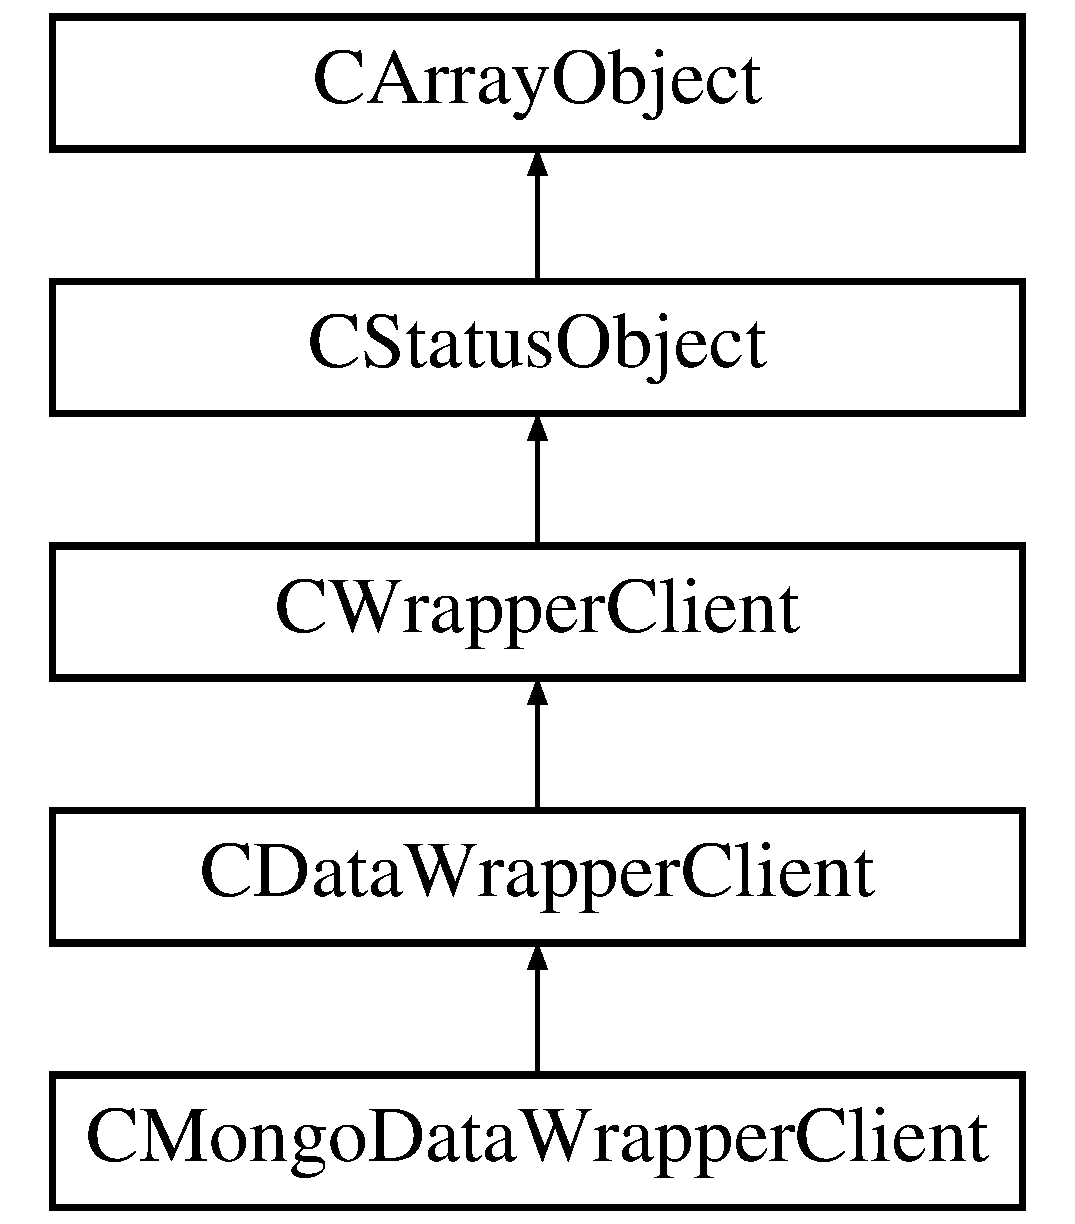
\includegraphics[height=5.000000cm]{class_c_mongo_data_wrapper_client}
\end{center}
\end{figure}
\subsection*{Public Member Functions}
\begin{DoxyCompactItemize}
\item 
\hyperlink{class_c_mongo_data_wrapper_client_a730c4fe3a66ad8a5aa42e44f669632ac}{Operation} (\$the\-Value=N\-U\-L\-L, \$get\-Old=F\-A\-L\-S\-E)
\item 
\hyperlink{class_c_mongo_data_wrapper_client_aba6b9751de7723443f54ad7f7b46897b}{No\-Response} (\$the\-Value=N\-U\-L\-L, \$get\-Old=F\-A\-L\-S\-E)
\end{DoxyCompactItemize}


\subsection{Member Function Documentation}
\hypertarget{class_c_mongo_data_wrapper_client_aba6b9751de7723443f54ad7f7b46897b}{\index{C\-Mongo\-Data\-Wrapper\-Client@{C\-Mongo\-Data\-Wrapper\-Client}!No\-Response@{No\-Response}}
\index{No\-Response@{No\-Response}!CMongoDataWrapperClient@{C\-Mongo\-Data\-Wrapper\-Client}}
\subsubsection[{No\-Response}]{\setlength{\rightskip}{0pt plus 5cm}C\-Mongo\-Data\-Wrapper\-Client\-::\-No\-Response (
\begin{DoxyParamCaption}
\item[{}]{\$the\-Value = {\ttfamily NULL}, }
\item[{}]{\$get\-Old = {\ttfamily FALSE}}
\end{DoxyParamCaption}
)}}\label{class_c_mongo_data_wrapper_client_aba6b9751de7723443f54ad7f7b46897b}
Manage no response switch.

This method can be used to manage the no \hyperlink{}{response} switch, it accepts a boolean which represents either the on/off value, or the requested operation\-:


\begin{DoxyItemize}
\item {\itshape N\-U\-L\-L}\-: Return the current value. 
\item {\itshape F\-A\-L\-S\-E}\-: Delete the current value. 
\item {\itshape other}\-: Set the value with the provided parameter. 
\end{DoxyItemize}

The second parameter is a boolean which if {\itshape T\-R\-U\-E} will return the {\itshape old} value when replacing values; if {\itshape F\-A\-L\-S\-E}, it will return the currently set value.


\begin{DoxyParams}[1]{Parameters}
integer & {\em \$the\-Value} & Value or operation. \\
\hline
boolean & {\em \$get\-Old} & T\-R\-U\-E get old value.\\
\hline
\end{DoxyParams}
public \begin{DoxyReturn}{Returns}
mixed
\end{DoxyReturn}
\hyperlink{class_c_attribute_a9d231a47718719fcd6c33f3d0ac91675}{C\-Attribute\-::\-Manage\-Offset()}

\begin{DoxySeeAlso}{See also}
k\-A\-P\-I\-\_\-\-O\-P\-T\-\_\-\-N\-O\-\_\-\-R\-E\-S\-P 
\end{DoxySeeAlso}
\hypertarget{class_c_mongo_data_wrapper_client_a730c4fe3a66ad8a5aa42e44f669632ac}{\index{C\-Mongo\-Data\-Wrapper\-Client@{C\-Mongo\-Data\-Wrapper\-Client}!Operation@{Operation}}
\index{Operation@{Operation}!CMongoDataWrapperClient@{C\-Mongo\-Data\-Wrapper\-Client}}
\subsubsection[{Operation}]{\setlength{\rightskip}{0pt plus 5cm}C\-Mongo\-Data\-Wrapper\-Client\-::\-Operation (
\begin{DoxyParamCaption}
\item[{}]{\$the\-Value = {\ttfamily NULL}, }
\item[{}]{\$get\-Old = {\ttfamily FALSE}}
\end{DoxyParamCaption}
)}}\label{class_c_mongo_data_wrapper_client_a730c4fe3a66ad8a5aa42e44f669632ac}
Manage operation.

We \hyperlink{class_c_data_wrapper_client_ae7cad4809c20d8f2871cfe00da909d67}{overload} this method to add the following allowed operations\-:


\begin{DoxyItemize}
\item {\itshape \hyperlink{}{k\-A\-P\-I\-\_\-\-O\-P\-\_\-\-G\-E\-T\-\_\-\-O\-N\-E}}\-: This is the tag that represents the find\-One Mongo operation, it will return the first matched object. 
\item {\itshape \hyperlink{}{k\-A\-P\-I\-\_\-\-O\-P\-\_\-\-G\-E\-T\-\_\-\-O\-B\-J\-E\-C\-T\-\_\-\-R\-E\-F}}\-: This tag defines a web-\/service that returns an object by reference. It is equivalent to the \hyperlink{}{k\-A\-P\-I\-\_\-\-O\-P\-\_\-\-G\-E\-T\-\_\-\-O\-N\-E} operation, except that instead of using the query provided in the \hyperlink{}{k\-A\-P\-I\-\_\-\-D\-A\-T\-A\-\_\-\-Q\-U\-E\-R\-Y} parameter, it will try to extract an identifier from the object provided in the \hyperlink{}{k\-A\-P\-I\-\_\-\-D\-A\-T\-A\-\_\-\-O\-B\-J\-E\-C\-T} parameter. 
\end{DoxyItemize}


\begin{DoxyParams}[1]{Parameters}
string & {\em \$the\-Value} & Value or operation. \\
\hline
boolean & {\em \$get\-Old} & T\-R\-U\-E get old value.\\
\hline
\end{DoxyParams}
public \begin{DoxyReturn}{Returns}
mixed
\end{DoxyReturn}

\begin{DoxyExceptions}{Exceptions}
{\em \{@link} & \hyperlink{class_c_exception}{C\-Exception} \hyperlink{class_c_exception}{C\-Exception}\}\\
\hline
\end{DoxyExceptions}
\hyperlink{class_c_attribute_a9d231a47718719fcd6c33f3d0ac91675}{C\-Attribute\-::\-Manage\-Offset()}

\begin{DoxySeeAlso}{See also}
k\-A\-P\-I\-\_\-\-O\-P\-E\-R\-A\-T\-I\-O\-N 

k\-A\-P\-I\-\_\-\-O\-P\-\_\-\-G\-E\-T\-\_\-\-O\-N\-E k\-A\-P\-I\-\_\-\-O\-P\-\_\-\-G\-E\-T\-\_\-\-O\-B\-J\-E\-C\-T\-\_\-\-R\-E\-F 
\end{DoxySeeAlso}


Reimplemented from \hyperlink{class_c_data_wrapper_client_ae7cad4809c20d8f2871cfe00da909d67}{C\-Data\-Wrapper\-Client}.



The documentation for this class was generated from the following file\-:\begin{DoxyCompactItemize}
\item 
/\-Library/\-Web\-Server/\-Library/wrapper/classes/C\-Mongo\-Data\-Wrapper\-Client.\-php\end{DoxyCompactItemize}

\hypertarget{class_c_mongo_query}{\section{C\-Mongo\-Query Class Reference}
\label{class_c_mongo_query}\index{C\-Mongo\-Query@{C\-Mongo\-Query}}
}
Inheritance diagram for C\-Mongo\-Query\-:\begin{figure}[H]
\begin{center}
\leavevmode
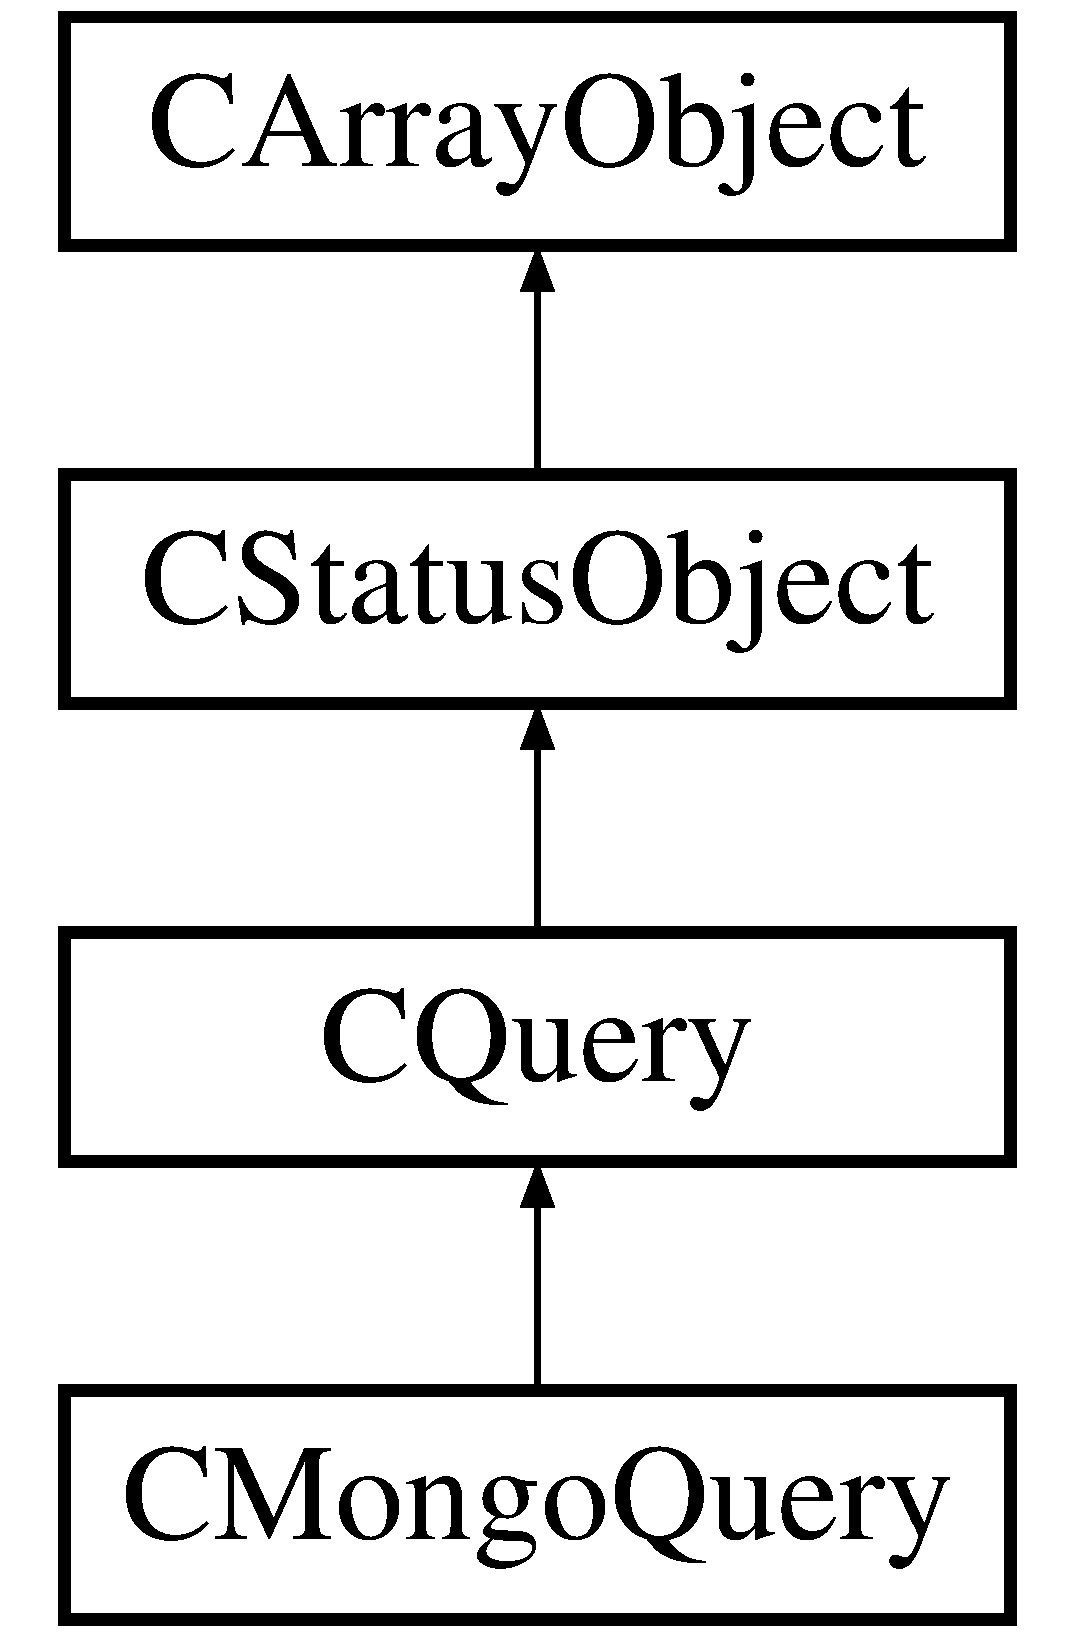
\includegraphics[height=4.000000cm]{class_c_mongo_query}
\end{center}
\end{figure}
\subsection*{Public Member Functions}
\begin{DoxyCompactItemize}
\item 
\hyperlink{class_c_mongo_query_aa25b073480c02f12b91bf262071fa884}{Export} (\$the\-Container)
\end{DoxyCompactItemize}
\subsection*{Protected Member Functions}
\begin{DoxyCompactItemize}
\item 
\hyperlink{class_c_mongo_query_a651af70656cb9894ef1885a711a0c141}{\-\_\-\-Validate\-Condition} (\$the\-Condition, \$the\-Statements, \$the\-Level)
\item 
\hyperlink{class_c_mongo_query_a8cda9306ac308f5c33456e77de004ebb}{\-\_\-\-Convert\-Condition} (\&\$the\-Query, \$the\-Container, \$the\-Condition, \$the\-Statements)
\item 
\hyperlink{class_c_mongo_query_a1f381db3f898f4c9cd333ffd2e3e989b}{\-\_\-\-Convert\-Statement} (\&\$the\-Query, \$the\-Container, \$the\-Condition, \$the\-Statement)
\item 
\hyperlink{class_c_mongo_query_a32fd372e1c39add42d078441eda3f1c3}{\-\_\-\-Order\-Range} (\$the\-Range, \hyperlink{class_c_mongo_container}{C\-Mongo\-Container} \$the\-Container, \$the\-Type)
\end{DoxyCompactItemize}


\subsection{Member Function Documentation}
\hypertarget{class_c_mongo_query_a8cda9306ac308f5c33456e77de004ebb}{\index{C\-Mongo\-Query@{C\-Mongo\-Query}!\-\_\-\-Convert\-Condition@{\-\_\-\-Convert\-Condition}}
\index{\-\_\-\-Convert\-Condition@{\-\_\-\-Convert\-Condition}!CMongoQuery@{C\-Mongo\-Query}}
\subsubsection[{\-\_\-\-Convert\-Condition}]{\setlength{\rightskip}{0pt plus 5cm}C\-Mongo\-Query\-::\-\_\-\-Convert\-Condition (
\begin{DoxyParamCaption}
\item[{\&}]{\$the\-Query, }
\item[{}]{\$the\-Container, }
\item[{}]{\$the\-Condition, }
\item[{}]{\$the\-Statements}
\end{DoxyParamCaption}
)\hspace{0.3cm}{\ttfamily [protected]}}}\label{class_c_mongo_query_a8cda9306ac308f5c33456e77de004ebb}
Convert condition.

This method will convert the statements of the provided condition to Mongo format.

The parameters to this method are\-:


\begin{DoxyItemize}
\item {\bfseries \&\$the\-Query}\-: Reference to an array that will receive the converted condition. 
\item {\bfseries \$the\-Container}\-: Data container, must be derived from \hyperlink{class_c_mongo_container}{C\-Mongo\-Container}. 
\item {\bfseries \$the\-Condition}\-: Boolean condition code. 
\item {\bfseries \$the\-Statements}\-: List of condition statements. 
\end{DoxyItemize}


\begin{DoxyParams}[1]{Parameters}
reference & {\em \&\$the\-Query} & Receives converted query. \\
\hline
\hyperlink{class_c_mongo_container}{C\-Mongo\-Container} & {\em \$the\-Container} & Query container. \\
\hline
string & {\em \$the\-Condition} & Boolean condition. \\
\hline
array & {\em \$the\-Statements} & Statements list.\\
\hline
\end{DoxyParams}
protected \hypertarget{class_c_mongo_query_a1f381db3f898f4c9cd333ffd2e3e989b}{\index{C\-Mongo\-Query@{C\-Mongo\-Query}!\-\_\-\-Convert\-Statement@{\-\_\-\-Convert\-Statement}}
\index{\-\_\-\-Convert\-Statement@{\-\_\-\-Convert\-Statement}!CMongoQuery@{C\-Mongo\-Query}}
\subsubsection[{\-\_\-\-Convert\-Statement}]{\setlength{\rightskip}{0pt plus 5cm}C\-Mongo\-Query\-::\-\_\-\-Convert\-Statement (
\begin{DoxyParamCaption}
\item[{\&}]{\$the\-Query, }
\item[{}]{\$the\-Container, }
\item[{}]{\$the\-Condition, }
\item[{}]{\$the\-Statement}
\end{DoxyParamCaption}
)\hspace{0.3cm}{\ttfamily [protected]}}}\label{class_c_mongo_query_a1f381db3f898f4c9cd333ffd2e3e989b}
Convert statement.

This method will convert the statement to Mongo format.

The parameters to this method are\-:


\begin{DoxyItemize}
\item {\bfseries \&\$the\-Query}\-: Reference to an array that will receive the converted statement. 
\item {\bfseries \$the\-Container}\-: Data container, must be derived from \hyperlink{class_c_mongo_container}{C\-Mongo\-Container} and we assume this check has been done by the \hyperlink{class_c_mongo_query_a8cda9306ac308f5c33456e77de004ebb}{caller}. 
\item {\bfseries \$the\-Condition}\-: Boolean condition code. 
\item {\bfseries \$the\-Statement}\-: Statement. 
\end{DoxyItemize}


\begin{DoxyParams}[1]{Parameters}
reference & {\em \&\$the\-Query} & Receives converted statement. \\
\hline
\hyperlink{class_c_mongo_container}{C\-Mongo\-Container} & {\em \$the\-Container} & Query container. \\
\hline
string & {\em \$the\-Condition} & Boolean condition. \\
\hline
array & {\em \$the\-Statement} & Statement.\\
\hline
\end{DoxyParams}
protected \hypertarget{class_c_mongo_query_a32fd372e1c39add42d078441eda3f1c3}{\index{C\-Mongo\-Query@{C\-Mongo\-Query}!\-\_\-\-Order\-Range@{\-\_\-\-Order\-Range}}
\index{\-\_\-\-Order\-Range@{\-\_\-\-Order\-Range}!CMongoQuery@{C\-Mongo\-Query}}
\subsubsection[{\-\_\-\-Order\-Range}]{\setlength{\rightskip}{0pt plus 5cm}C\-Mongo\-Query\-::\-\_\-\-Order\-Range (
\begin{DoxyParamCaption}
\item[{}]{\$the\-Range, }
\item[{{\bf C\-Mongo\-Container}}]{\$the\-Container, }
\item[{}]{\$the\-Type}
\end{DoxyParamCaption}
)\hspace{0.3cm}{\ttfamily [protected]}}}\label{class_c_mongo_query_a32fd372e1c39add42d078441eda3f1c3}
Order range elements.

This method will order the provided range elements, the method accepts an array of two elements which represent the range bounds and will return an array with the two provided elements sorted.

The method accepts three parameters\-:


\begin{DoxyItemize}
\item {\bfseries \$the\-Range}\-: An array containing two elements representing the range bounds. 
\item {\bfseries \$the\-Container}\-: The \hyperlink{class_c_mongo_container}{container} on which the query will be executed. 
\item {\bfseries \$the\-Type}\-: The data type of the range elements. 
\end{DoxyItemize}

The method expects the range elements to be in \hyperlink{class_c_data_type_a1cae522eec386d293b6087a99e9a8b0b}{serialised} format, these elements will be \hyperlink{class_c_container_a09d585e2a9809221a42d52d7520c9cbf}{converted} by this method which will return them in sorted order.


\begin{DoxyParams}[1]{Parameters}
mixed & {\em \$the\-Range} & Range elements. \\
\hline
C\-Mongo\-Comtainer & {\em \$the\-Container} & Query container. \\
\hline
string & {\em \$the\-Type} & Elements data type.\\
\hline
\end{DoxyParams}
protected \begin{DoxyReturn}{Returns}
array 
\end{DoxyReturn}
\hypertarget{class_c_mongo_query_a651af70656cb9894ef1885a711a0c141}{\index{C\-Mongo\-Query@{C\-Mongo\-Query}!\-\_\-\-Validate\-Condition@{\-\_\-\-Validate\-Condition}}
\index{\-\_\-\-Validate\-Condition@{\-\_\-\-Validate\-Condition}!CMongoQuery@{C\-Mongo\-Query}}
\subsubsection[{\-\_\-\-Validate\-Condition}]{\setlength{\rightskip}{0pt plus 5cm}C\-Mongo\-Query\-::\-\_\-\-Validate\-Condition (
\begin{DoxyParamCaption}
\item[{}]{\$the\-Condition, }
\item[{}]{\$the\-Statements, }
\item[{}]{\$the\-Level}
\end{DoxyParamCaption}
)\hspace{0.3cm}{\ttfamily [protected]}}}\label{class_c_mongo_query_a651af70656cb9894ef1885a711a0c141}
Validate condition.

This method expects a condition as its argument, it will check if it is a valid condition, then it will \hyperlink{class_c_query_afe96707c9ed84ee197dae56c9f05f2a4}{validate} all condition statements.

In this class we handle queries to Mongo databases, so the depth of the query conditions cannot go beyond 2 levels.

We overload this method to prevent nesting O\-R conditions.


\begin{DoxyParams}[1]{Parameters}
string & {\em \$the\-Condition} & Boolean condition. \\
\hline
array & {\em \$the\-Statements} & Statements list. \\
\hline
integer & {\em \$the\-Level} & \mbox{[}P\-R\-I\-V\-A\-T\-E\mbox{]} condition level.\\
\hline
\end{DoxyParams}
protected 

Reimplemented from \hyperlink{class_c_query_a5fbde46df4bb30cb252647f0e47cbbde}{C\-Query}.

\hypertarget{class_c_mongo_query_aa25b073480c02f12b91bf262071fa884}{\index{C\-Mongo\-Query@{C\-Mongo\-Query}!Export@{Export}}
\index{Export@{Export}!CMongoQuery@{C\-Mongo\-Query}}
\subsubsection[{Export}]{\setlength{\rightskip}{0pt plus 5cm}C\-Mongo\-Query\-::\-Export (
\begin{DoxyParamCaption}
\item[{}]{\$the\-Container}
\end{DoxyParamCaption}
)}}\label{class_c_mongo_query_aa25b073480c02f12b91bf262071fa884}
Export query.

The method will return an array suitable to be provided as a Mongo\-D\-B query, the method requires a container that will take care of converting query arguments to native data types, this container must be an instance of \hyperlink{class_c_mongo_container}{C\-Mongo\-Container}, or the method will raise an exception.


\begin{DoxyParams}[1]{Parameters}
\hyperlink{class_c_mongo_container}{C\-Mongo\-Container} & {\em \$the\-Container} & Query container.\\
\hline
\end{DoxyParams}
public \begin{DoxyReturn}{Returns}
array
\end{DoxyReturn}

\begin{DoxyExceptions}{Exceptions}
{\em Exception} & \\
\hline
\end{DoxyExceptions}


The documentation for this class was generated from the following file\-:\begin{DoxyCompactItemize}
\item 
/\-Library/\-Web\-Server/\-Library/wrapper/classes/C\-Mongo\-Query.\-php\end{DoxyCompactItemize}

\hypertarget{class_c_object}{\section{C\-Object Class Reference}
\label{class_c_object}\index{C\-Object@{C\-Object}}
}
Inheritance diagram for C\-Object\-:\begin{figure}[H]
\begin{center}
\leavevmode
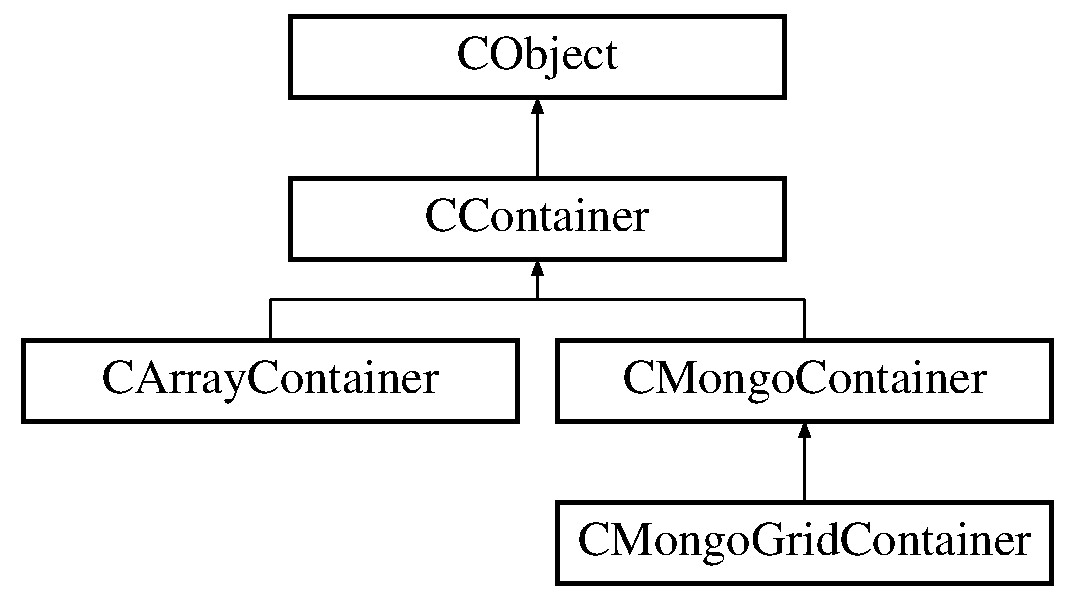
\includegraphics[height=4.000000cm]{class_c_object}
\end{center}
\end{figure}
\subsection*{Static Public Member Functions}
\begin{DoxyCompactItemize}
\item 
static \hyperlink{class_c_object_a660f66b5be21d0cd1156463bcf75e575}{Json\-Encode} (\$the\-Data)
\item 
static \hyperlink{class_c_object_a06eb0f5acf83d67bda8f7946cade841e}{Json\-Decode} (\$the\-Data)
\item 
static \hyperlink{class_c_object_a3c28f63ed5bf37b96c15008f8c825628}{String\-Normalise} (\$the\-String, \$the\-Modifiers=k\-F\-L\-A\-G\-\_\-\-D\-E\-F\-A\-U\-L\-T)
\item 
static \hyperlink{class_c_object_a0255e495d3d0485b50988e496b0249c6}{Duration\-String} (\$the\-Time)
\item 
static \hyperlink{class_c_object_a9b8dccdadcf4fea58f915bd9b228e23e}{Manage\-Member} (\&\$the\-Member, \$the\-Value=N\-U\-L\-L, \$get\-Old=F\-A\-L\-S\-E)
\end{DoxyCompactItemize}


\subsection{Member Function Documentation}
\hypertarget{class_c_object_a0255e495d3d0485b50988e496b0249c6}{\index{C\-Object@{C\-Object}!Duration\-String@{Duration\-String}}
\index{Duration\-String@{Duration\-String}!CObject@{C\-Object}}
\subsubsection[{Duration\-String}]{\setlength{\rightskip}{0pt plus 5cm}static C\-Object\-::\-Duration\-String (
\begin{DoxyParamCaption}
\item[{}]{\$the\-Time}
\end{DoxyParamCaption}
)\hspace{0.3cm}{\ttfamily [static]}}}\label{class_c_object_a0255e495d3d0485b50988e496b0249c6}
Return a formatted duration.

This function will return a formatted duration string in H\-:\-M\-M\-:\-S\-S\-:mmmmm format, where {\itshape H} stands for hours, {\itshape M} stands for minutes, {\itshape S} stands for seconds and {\itshape m} stands for milliseconds, from the value of {\itshape microtime( T\-R\-U\-E )}.

{\itshape Note\-: The provided value should be a difference between two timestamps taken with microtime( true ).}


\begin{DoxyParams}[1]{Parameters}
float & {\em \$the\-Time} & Microtime difference.\\
\hline
\end{DoxyParams}
\begin{DoxyReturn}{Returns}
string 
\end{DoxyReturn}
\hypertarget{class_c_object_a06eb0f5acf83d67bda8f7946cade841e}{\index{C\-Object@{C\-Object}!Json\-Decode@{Json\-Decode}}
\index{Json\-Decode@{Json\-Decode}!CObject@{C\-Object}}
\subsubsection[{Json\-Decode}]{\setlength{\rightskip}{0pt plus 5cm}static C\-Object\-::\-Json\-Decode (
\begin{DoxyParamCaption}
\item[{}]{\$the\-Data}
\end{DoxyParamCaption}
)\hspace{0.3cm}{\ttfamily [static]}}}\label{class_c_object_a06eb0f5acf83d67bda8f7946cade841e}
Return J\-S\-O\-N decoded data.

This method will return an array representation of the provided J\-S\-O\-N string.


\begin{DoxyParams}[1]{Parameters}
string & {\em \$the\-Data} & Input data.\\
\hline
\end{DoxyParams}
\begin{DoxyReturn}{Returns}
array 
\end{DoxyReturn}
\hypertarget{class_c_object_a660f66b5be21d0cd1156463bcf75e575}{\index{C\-Object@{C\-Object}!Json\-Encode@{Json\-Encode}}
\index{Json\-Encode@{Json\-Encode}!CObject@{C\-Object}}
\subsubsection[{Json\-Encode}]{\setlength{\rightskip}{0pt plus 5cm}static C\-Object\-::\-Json\-Encode (
\begin{DoxyParamCaption}
\item[{}]{\$the\-Data}
\end{DoxyParamCaption}
)\hspace{0.3cm}{\ttfamily [static]}}}\label{class_c_object_a660f66b5be21d0cd1156463bcf75e575}
Return J\-S\-O\-N encoded data.

This method will return the provided array or object into a J\-S\-O\-N encoded string.


\begin{DoxyParams}[1]{Parameters}
mixed & {\em \$the\-Data} & Input data.\\
\hline
\end{DoxyParams}
\begin{DoxyReturn}{Returns}
string 
\end{DoxyReturn}
\hypertarget{class_c_object_a9b8dccdadcf4fea58f915bd9b228e23e}{\index{C\-Object@{C\-Object}!Manage\-Member@{Manage\-Member}}
\index{Manage\-Member@{Manage\-Member}!CObject@{C\-Object}}
\subsubsection[{Manage\-Member}]{\setlength{\rightskip}{0pt plus 5cm}static C\-Object\-::\-Manage\-Member (
\begin{DoxyParamCaption}
\item[{\&}]{\$the\-Member, }
\item[{}]{\$the\-Value = {\ttfamily NULL}, }
\item[{}]{\$get\-Old = {\ttfamily FALSE}}
\end{DoxyParamCaption}
)\hspace{0.3cm}{\ttfamily [static]}}}\label{class_c_object_a9b8dccdadcf4fea58f915bd9b228e23e}
Manage a member.

This library implements a standard interface for managing object properties using methods, this method implements this interface\-:


\begin{DoxyItemize}
\item {\bfseries \$the\-Member}\-: The member to manage, it is a reference to the element being managed. 
\item {\bfseries \$the\-Value}\-: The value or operation\-: 
\begin{DoxyItemize}
\item {\itshape N\-U\-L\-L}\-: Return the member's current value. 
\item {\itshape F\-A\-L\-S\-E}\-: Reset the member, {\itshape N\-U\-L\-L} by default. 
\item {\itshape other}\-: Any other type represents the member's new value. 
\end{DoxyItemize}
\item {\bfseries \$get\-Old}\-: Determines what the method will return\-: 
\begin{DoxyItemize}
\item {\itshape T\-R\-U\-E}\-: Return the value of the member {\itshape before} it was eventually modified. 
\item {\itshape F\-A\-L\-S\-E}\-: Return the value of the member {\itshape after} it was eventually modified. 
\end{DoxyItemize}
\end{DoxyItemize}


\begin{DoxyParams}[1]{Parameters}
string & {\em \&\$the\-Member} & Offset. \\
\hline
mixed & {\em \$the\-Value} & Value or operation. \\
\hline
boolean & {\em \$get\-Old} & T\-R\-U\-E get old value.\\
\hline
\end{DoxyParams}
\begin{DoxyReturn}{Returns}
mixed 
\end{DoxyReturn}
\hypertarget{class_c_object_a3c28f63ed5bf37b96c15008f8c825628}{\index{C\-Object@{C\-Object}!String\-Normalise@{String\-Normalise}}
\index{String\-Normalise@{String\-Normalise}!CObject@{C\-Object}}
\subsubsection[{String\-Normalise}]{\setlength{\rightskip}{0pt plus 5cm}static C\-Object\-::\-String\-Normalise (
\begin{DoxyParamCaption}
\item[{}]{\$the\-String, }
\item[{}]{\$the\-Modifiers = {\ttfamily kFLAG\-\_\-DEFAULT}}
\end{DoxyParamCaption}
)\hspace{0.3cm}{\ttfamily [static]}}}\label{class_c_object_a3c28f63ed5bf37b96c15008f8c825628}
Normalise string.

This method can be used to format a string, the provided modifiers bitfield determines what manipulations are applied\-:


\begin{DoxyItemize}
\item {\bfseries \hyperlink{}{k\-F\-L\-A\-G\-\_\-\-M\-O\-D\-I\-F\-I\-E\-R\-\_\-\-U\-T\-F8}}\-: Convert the string to the {\itshape U\-T\-F8} character set. 
\item {\bfseries \hyperlink{}{k\-F\-L\-A\-G\-\_\-\-M\-O\-D\-I\-F\-I\-E\-R\-\_\-\-L\-T\-R\-I\-M}}\-: Apply left trimming to the string. 
\item {\bfseries \hyperlink{}{k\-F\-L\-A\-G\-\_\-\-M\-O\-D\-I\-F\-I\-E\-R\-\_\-\-R\-T\-R\-I\-M}}\-: Apply right trimming to the string. 
\item {\bfseries \hyperlink{}{k\-F\-L\-A\-G\-\_\-\-M\-O\-D\-I\-F\-I\-E\-R\-\_\-\-T\-R\-I\-M}}\-: Apply both left and right trimming to the string. 
\item {\bfseries \hyperlink{}{k\-F\-L\-A\-G\-\_\-\-M\-O\-D\-I\-F\-I\-E\-R\-\_\-\-N\-U\-L\-L}}\-: If this flag is set and the resulting string is empty, the method will return {\itshape N\-U\-L\-L}. 
\begin{DoxyItemize}
\item {\bfseries \hyperlink{}{k\-F\-L\-A\-G\-\_\-\-M\-O\-D\-I\-F\-I\-E\-R\-\_\-\-N\-U\-L\-L\-S\-T\-R}}\-: If this flag is set and the resulting string is empty, the method will return the '{\itshape N\-U\-L\-L}' string; this option implies that the \hyperlink{}{k\-F\-L\-A\-G\-\_\-\-M\-O\-D\-I\-F\-I\-E\-R\-\_\-\-N\-U\-L\-L} is also set. 
\end{DoxyItemize}
\item {\bfseries \hyperlink{}{k\-F\-L\-A\-G\-\_\-\-M\-O\-D\-I\-F\-I\-E\-R\-\_\-\-N\-O\-C\-A\-S\-E}}\-: Set the string to lowercase, this is the default way to generate a case insensitive string. 
\item {\bfseries \hyperlink{}{k\-F\-L\-A\-G\-\_\-\-M\-O\-D\-I\-F\-I\-E\-R\-\_\-\-U\-R\-L}}\-: U\-R\-L-\/encode the string; note that this option and \hyperlink{}{k\-F\-L\-A\-G\-\_\-\-M\-O\-D\-I\-F\-I\-E\-R\-\_\-\-H\-T\-M\-L} are mutually exclusive. 
\item {\bfseries \hyperlink{}{k\-F\-L\-A\-G\-\_\-\-M\-O\-D\-I\-F\-I\-E\-R\-\_\-\-H\-T\-M\-L}}\-: H\-T\-M\-L-\/encode the string; note that this option and \hyperlink{}{k\-F\-L\-A\-G\-\_\-\-M\-O\-D\-I\-F\-I\-E\-R\-\_\-\-U\-R\-L} are mutually exclusive. 
\item {\bfseries \hyperlink{}{k\-F\-L\-A\-G\-\_\-\-M\-O\-D\-I\-F\-I\-E\-R\-\_\-\-H\-E\-X}}\-: Convert the string to hexadecimal; note that this option and \hyperlink{}{hashing} are mutually exclusive. 
\begin{DoxyItemize}
\item {\bfseries \hyperlink{}{k\-F\-L\-A\-G\-\_\-\-M\-O\-D\-I\-F\-I\-E\-R\-\_\-\-H\-E\-X\-E\-X\-P}}\-: Convert the string to a hexadecimal expression; note that this option implies \hyperlink{}{k\-F\-L\-A\-G\-\_\-\-M\-O\-D\-I\-F\-I\-E\-R\-\_\-\-H\-E\-X}, and this option and \hyperlink{}{hashing} are mutually exclusive. 
\end{DoxyItemize}
\item {\bfseries \hyperlink{}{k\-F\-L\-A\-G\-\_\-\-M\-O\-D\-I\-F\-I\-E\-R\-\_\-\-H\-A\-S\-H}}\-: If this bit is set the resulting string will be hashed using the {\itshape md5} algorithm resulting in a 32 character hexadecimal string; this option is mutually exclusive with the \hyperlink{}{k\-F\-L\-A\-G\-\_\-\-M\-O\-D\-I\-F\-I\-E\-R\-\_\-\-M\-A\-S\-K\-\_\-\-H\-E\-X} option. 
\begin{DoxyItemize}
\item {\bfseries \hyperlink{}{k\-F\-L\-A\-G\-\_\-\-M\-O\-D\-I\-F\-I\-E\-R\-\_\-\-H\-A\-S\-H\-\_\-\-B\-I\-N}}\-: If this bit is set, the resulting value should be a 16 character binary string; if the bit is {\itshape O\-F\-F}, the resulting value should be a 32 character hexadecimal string. 
\end{DoxyItemize}
\end{DoxyItemize}

The order in which these modifications are applied are as stated.


\begin{DoxyParams}[1]{Parameters}
string & {\em \$the\-String} & String to normalise. \\
\hline
bitfield & {\em \$the\-Modifiers} & Modifiers bitfield.\\
\hline
\end{DoxyParams}
\begin{DoxyReturn}{Returns}
mixed
\end{DoxyReturn}
\begin{DoxySeeAlso}{See Also}
k\-F\-L\-A\-G\-\_\-\-D\-E\-F\-A\-U\-L\-T, k\-F\-L\-A\-G\-\_\-\-M\-O\-D\-I\-F\-I\-E\-R\-\_\-\-M\-A\-S\-K 

k\-F\-L\-A\-G\-\_\-\-M\-O\-D\-I\-F\-I\-E\-R\-\_\-\-U\-T\-F8 

k\-F\-L\-A\-G\-\_\-\-M\-O\-D\-I\-F\-I\-E\-R\-\_\-\-L\-T\-R\-I\-M, k\-F\-L\-A\-G\-\_\-\-M\-O\-D\-I\-F\-I\-E\-R\-\_\-\-R\-T\-R\-I\-M, k\-F\-L\-A\-G\-\_\-\-M\-O\-D\-I\-F\-I\-E\-R\-\_\-\-T\-R\-I\-M 

k\-F\-L\-A\-G\-\_\-\-M\-O\-D\-I\-F\-I\-E\-R\-\_\-\-N\-U\-L\-L, k\-F\-L\-A\-G\-\_\-\-M\-O\-D\-I\-F\-I\-E\-R\-\_\-\-N\-U\-L\-L\-S\-T\-R 

k\-F\-L\-A\-G\-\_\-\-M\-O\-D\-I\-F\-I\-E\-R\-\_\-\-N\-O\-C\-A\-S\-E, k\-F\-L\-A\-G\-\_\-\-M\-O\-D\-I\-F\-I\-E\-R\-\_\-\-U\-R\-L, k\-F\-L\-A\-G\-\_\-\-M\-O\-D\-I\-F\-I\-E\-R\-\_\-\-H\-T\-M\-L 

k\-F\-L\-A\-G\-\_\-\-M\-O\-D\-I\-F\-I\-E\-R\-\_\-\-H\-E\-X, k\-F\-L\-A\-G\-\_\-\-M\-O\-D\-I\-F\-I\-E\-R\-\_\-\-H\-E\-X\-E\-X\-P 

k\-F\-L\-A\-G\-\_\-\-M\-O\-D\-I\-F\-I\-E\-R\-\_\-\-H\-A\-S\-H, k\-F\-L\-A\-G\-\_\-\-M\-O\-D\-I\-F\-I\-E\-R\-\_\-\-H\-A\-S\-H\-\_\-\-B\-I\-N 
\end{DoxySeeAlso}


The documentation for this class was generated from the following file\-:\begin{DoxyCompactItemize}
\item 
/\-Library/\-Web\-Server/\-Library/wrapper/classes/C\-Object.\-php\end{DoxyCompactItemize}

\hypertarget{class_c_ontology_edge}{\section{C\-Ontology\-Edge Class Reference}
\label{class_c_ontology_edge}\index{C\-Ontology\-Edge@{C\-Ontology\-Edge}}
}
Inheritance diagram for C\-Ontology\-Edge\-:\begin{figure}[H]
\begin{center}
\leavevmode
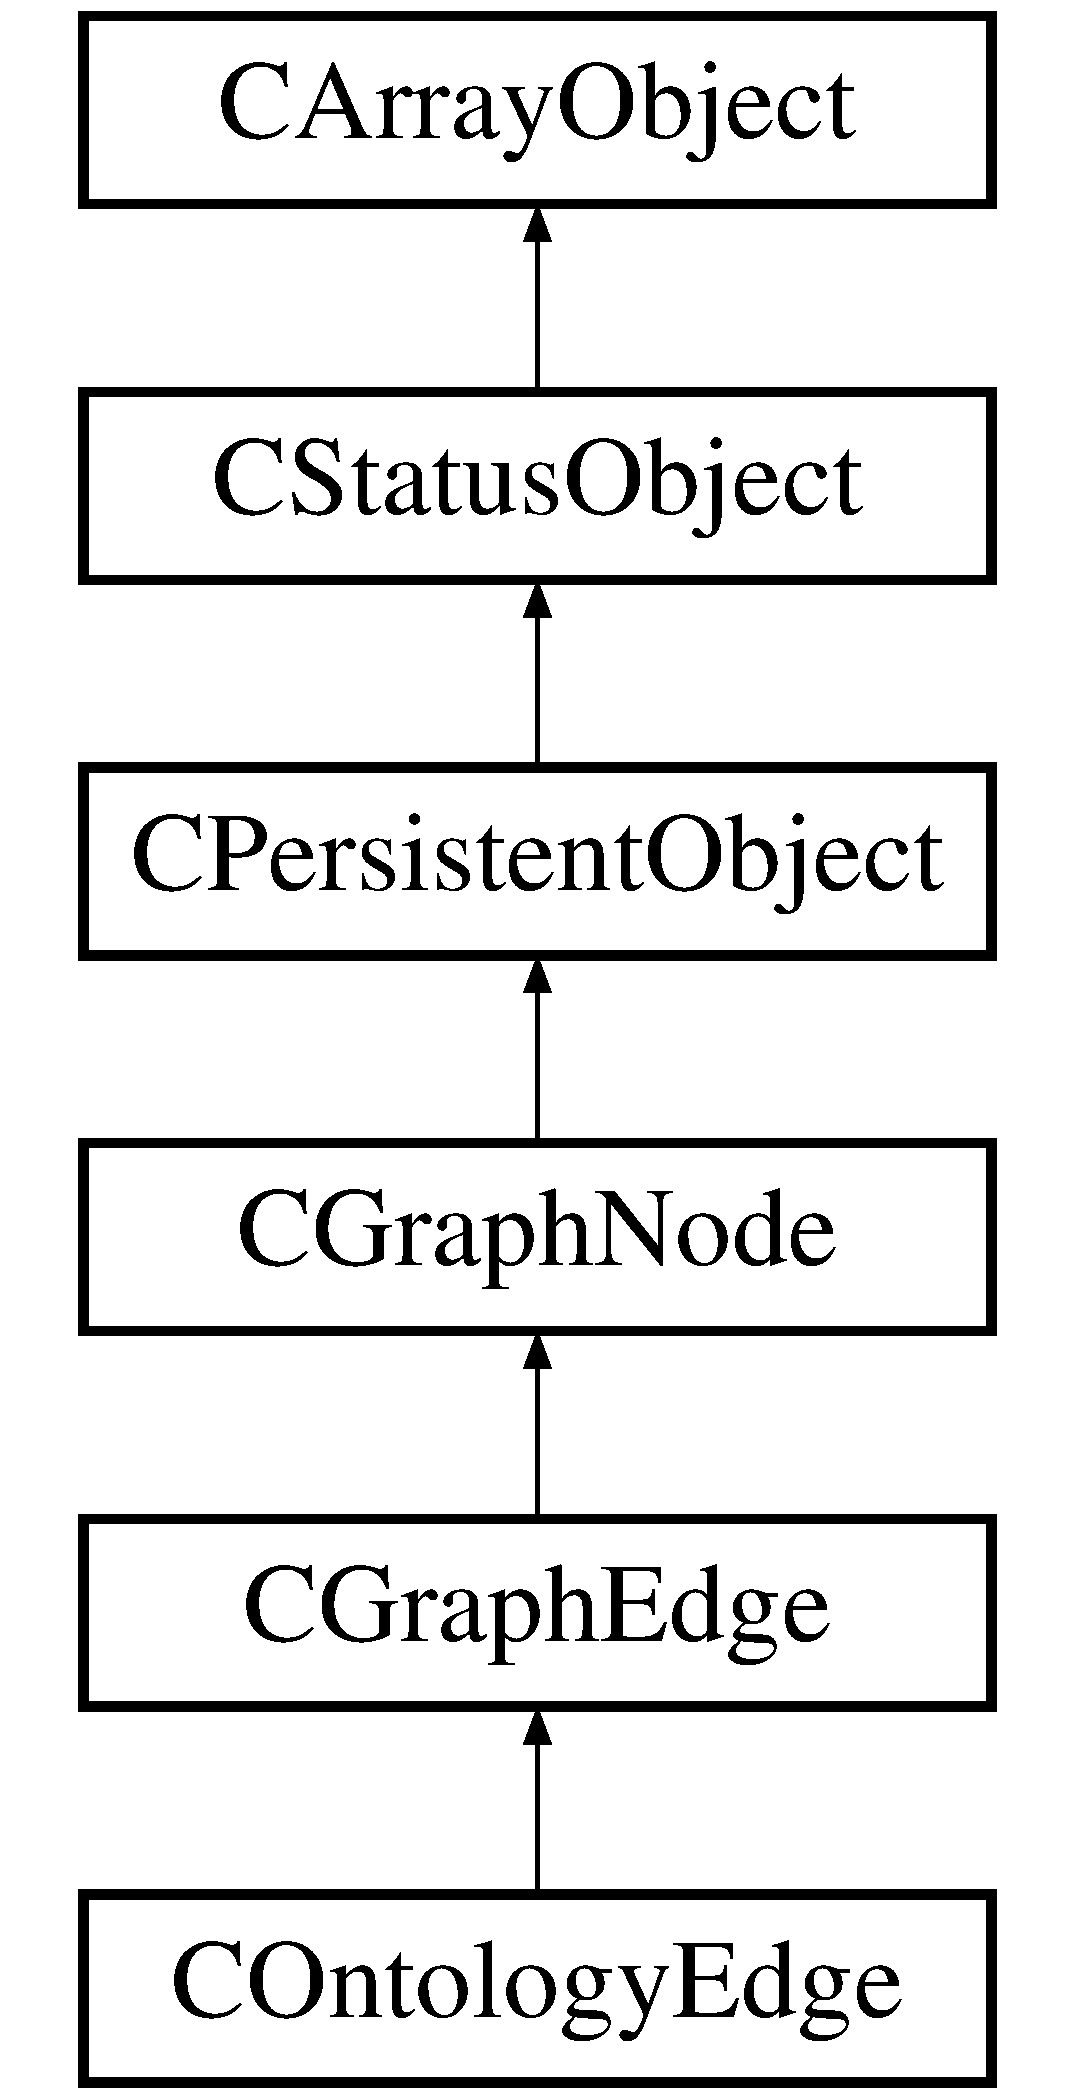
\includegraphics[height=6.000000cm]{class_c_ontology_edge}
\end{center}
\end{figure}
\subsection*{Public Member Functions}
\begin{DoxyCompactItemize}
\item 
\hyperlink{class_c_ontology_edge_acc739f853b1e64a3a36926dfd83fe7b4}{Term} (\$the\-Value=N\-U\-L\-L, \$get\-Old=F\-A\-L\-S\-E)
\item 
\hyperlink{class_c_ontology_edge_a3196d6612dbbbbbe18643b1af06378b4}{Subject\-Term} (\$the\-Value=N\-U\-L\-L, \$get\-Old=F\-A\-L\-S\-E)
\item 
\hyperlink{class_c_ontology_edge_a83ac612393cc615101992972b419faa5}{Object\-Term} (\$the\-Value=N\-U\-L\-L, \$get\-Old=F\-A\-L\-S\-E)
\item 
\hyperlink{class_c_ontology_edge_a68efd237a5a6079dc5c679183192d2dc}{Subject\-Node} (\$the\-Container)
\item 
\hyperlink{class_c_ontology_edge_a116f7950d0e7d744e12156c7f244b7b0}{Object\-Node} (\$the\-Container)
\item 
\hyperlink{class_c_ontology_edge_a009263d75d6128d2b62d6294febe6d02}{offset\-Exists} (\$the\-Offset)
\item 
\hyperlink{class_c_ontology_edge_a371744cd3e3bb699c12dad85c6ea3e54}{offset\-Get} (\$the\-Offset)
\item 
\hyperlink{class_c_ontology_edge_a8844ca89c568f127ab4e16fe9552c85b}{count} ()
\item 
\hyperlink{class_c_ontology_edge_a5661a9878ca8028bd656ecc7b193b26a}{get\-Array\-Copy} ()
\end{DoxyCompactItemize}
\subsection*{Protected Member Functions}
\begin{DoxyCompactItemize}
\item 
\hyperlink{class_c_ontology_edge_a76e551f21dcac3c0bc228c67226bec08}{\-\_\-\-Commit} (\&\$the\-Container, \&\$the\-Identifier, \&\$the\-Modifiers)
\item 
\hyperlink{class_c_ontology_edge_ae7a4861887c1a73dcdbd0285cdba1d8d}{\-\_\-\-Load} (\&\$the\-Container, \&\$the\-Identifier, \&\$the\-Modifiers)
\item 
\hyperlink{class_c_ontology_edge_a1d09b3ef8e4ef57a072291a7c09f7371}{\-\_\-\-Prepare\-Create} (\&\$the\-Container, \&\$the\-Identifier, \&\$the\-Modifiers)
\item 
\hyperlink{class_c_ontology_edge_a6099442ba1dca683e4832d406793b5b9}{\-\_\-\-Prepare\-Load} (\&\$the\-Container, \&\$the\-Identifier, \&\$the\-Modifiers)
\item 
\hyperlink{class_c_ontology_edge_a2bea996dff6e836069d75572f9386039}{\-\_\-\-Prepare\-Commit} (\&\$the\-Container, \&\$the\-Identifier, \&\$the\-Modifiers)
\item 
\hyperlink{class_c_ontology_edge_a0956d5920484a329c77d878bb6c25784}{\-\_\-\-Finish\-Create} (\&\$the\-Container)
\item 
\hyperlink{class_c_ontology_edge_ac45af3396c797be599c2a1780b7bfa59}{\-\_\-\-Finish\-Load} (\&\$the\-Container, \&\$the\-Identifier, \&\$the\-Modifiers)
\item 
\hyperlink{class_c_ontology_edge_a7b8a93f340be66aa47e6e1e73ff326ab}{\-\_\-\-Index\-Terms} (Everyman\textbackslash{}\-Neo4j\textbackslash{}\-Client \$the\-Container)
\item 
\hyperlink{class_c_ontology_edge_ab047f9ba598226fe20c268239aacb727}{\-\_\-\-Get\-Node\-Index} (Everyman\textbackslash{}\-Neo4j\textbackslash{}\-Client \$the\-Container, \$the\-Index, \$do\-Clear=F\-A\-L\-S\-E)
\end{DoxyCompactItemize}
\subsection*{Protected Attributes}
\begin{DoxyCompactItemize}
\item 
\hypertarget{class_c_ontology_edge_a7da276bc73676096b1cef4cdbf88428b}{{\bfseries \$m\-Predicate\-Term} = N\-U\-L\-L}\label{class_c_ontology_edge_a7da276bc73676096b1cef4cdbf88428b}

\item 
\hypertarget{class_c_ontology_edge_af9c4f23f64990824355d21daf3db1a1a}{{\bfseries \$m\-Subject\-Term} = N\-U\-L\-L}\label{class_c_ontology_edge_af9c4f23f64990824355d21daf3db1a1a}

\item 
\hypertarget{class_c_ontology_edge_a2dabe441063537fdd713b6cda8064688}{{\bfseries \$m\-Object\-Term} = N\-U\-L\-L}\label{class_c_ontology_edge_a2dabe441063537fdd713b6cda8064688}

\end{DoxyCompactItemize}


\subsection{Member Function Documentation}
\hypertarget{class_c_ontology_edge_a76e551f21dcac3c0bc228c67226bec08}{\index{C\-Ontology\-Edge@{C\-Ontology\-Edge}!\-\_\-\-Commit@{\-\_\-\-Commit}}
\index{\-\_\-\-Commit@{\-\_\-\-Commit}!COntologyEdge@{C\-Ontology\-Edge}}
\subsubsection[{\-\_\-\-Commit}]{\setlength{\rightskip}{0pt plus 5cm}C\-Ontology\-Edge\-::\-\_\-\-Commit (
\begin{DoxyParamCaption}
\item[{\&}]{\$the\-Container, }
\item[{\&}]{\$the\-Identifier, }
\item[{\&}]{\$the\-Modifiers}
\end{DoxyParamCaption}
)\hspace{0.3cm}{\ttfamily [protected]}}}\label{class_c_ontology_edge_a76e551f21dcac3c0bc228c67226bec08}
Store object in container.

We \hyperlink{class_c_graph_edge_a73dd2ced3103285f8ad4ea212c0e918e}{overload} this method to provide the correct container to the \hyperlink{class_c_graph_edge}{parent} \hyperlink{class_c_graph_edge_a73dd2ced3103285f8ad4ea212c0e918e}{method}.

We also \hyperlink{class_c_persistent_object_a88b1f2b11d3d60e0b3d33d8b0649b68a}{commit} the \hyperlink{class_c_ontology_edge_a3196d6612dbbbbbe18643b1af06378b4}{subject} and \hyperlink{class_c_ontology_edge_a83ac612393cc615101992972b419faa5}{object} \hyperlink{class_c_ontology_term}{terms}, setting or removing \hyperlink{class_c_ontology_term}{their} \hyperlink{}{k\-T\-A\-G\-\_\-\-N\-O\-D\-Enode} reference.

We also overload this method to store the node properties into a Mongo collection named \hyperlink{}{k\-D\-E\-F\-A\-U\-L\-T\-\_\-\-C\-N\-T\-\_\-\-E\-D\-G\-E\-S}, the record will be indexed by the combination of subject and node I\-Ds interleaved with the predicate term \hyperlink{}{identifier} and divided by the \hyperlink{}{k\-T\-O\-K\-E\-N\-\_\-\-I\-N\-D\-E\-X\-\_\-\-S\-E\-P\-A\-R\-A\-T\-O\-R} token.


\begin{DoxyParams}[1]{Parameters}
reference & {\em \&\$the\-Container} & Object container. \\
\hline
reference & {\em \&\$the\-Identifier} & Object identifier. \\
\hline
reference & {\em \&\$the\-Modifiers} & Commit modifiers.\\
\hline
\end{DoxyParams}
protected \begin{DoxyReturn}{Returns}
mixed
\end{DoxyReturn}
\hyperlink{class_c_graph_edge_a6606e13ba79ab94fc0db50bef197d416}{Node()} 

Reimplemented from \hyperlink{class_c_graph_edge_a73dd2ced3103285f8ad4ea212c0e918e}{C\-Graph\-Edge}.

\hypertarget{class_c_ontology_edge_a0956d5920484a329c77d878bb6c25784}{\index{C\-Ontology\-Edge@{C\-Ontology\-Edge}!\-\_\-\-Finish\-Create@{\-\_\-\-Finish\-Create}}
\index{\-\_\-\-Finish\-Create@{\-\_\-\-Finish\-Create}!COntologyEdge@{C\-Ontology\-Edge}}
\subsubsection[{\-\_\-\-Finish\-Create}]{\setlength{\rightskip}{0pt plus 5cm}C\-Ontology\-Edge\-::\-\_\-\-Finish\-Create (
\begin{DoxyParamCaption}
\item[{\&}]{\$the\-Container}
\end{DoxyParamCaption}
)\hspace{0.3cm}{\ttfamily [protected]}}}\label{class_c_ontology_edge_a0956d5920484a329c77d878bb6c25784}
Normalise after a \hyperlink{class_c_graph_node_a90e49bf5e95ccf3c8644196696154268}{create}.

In this class we initialise the \hyperlink{class_c_ontology_edge_acc739f853b1e64a3a36926dfd83fe7b4}{predicate}, \hyperlink{class_c_ontology_edge_a3196d6612dbbbbbe18643b1af06378b4}{subject} and \hyperlink{class_c_ontology_edge_a83ac612393cc615101992972b419faa5}{object} \hyperlink{class_c_ontology_term}{terms}.


\begin{DoxyParams}[1]{Parameters}
reference & {\em \&\$the\-Container} & Object container.\\
\hline
\end{DoxyParams}
protected 

Reimplemented from \hyperlink{class_c_graph_edge_a42fd83eff1eef079a6005e961fd2d371}{C\-Graph\-Edge}.

\hypertarget{class_c_ontology_edge_ac45af3396c797be599c2a1780b7bfa59}{\index{C\-Ontology\-Edge@{C\-Ontology\-Edge}!\-\_\-\-Finish\-Load@{\-\_\-\-Finish\-Load}}
\index{\-\_\-\-Finish\-Load@{\-\_\-\-Finish\-Load}!COntologyEdge@{C\-Ontology\-Edge}}
\subsubsection[{\-\_\-\-Finish\-Load}]{\setlength{\rightskip}{0pt plus 5cm}C\-Ontology\-Edge\-::\-\_\-\-Finish\-Load (
\begin{DoxyParamCaption}
\item[{\&}]{\$the\-Container, }
\item[{\&}]{\$the\-Identifier, }
\item[{\&}]{\$the\-Modifiers}
\end{DoxyParamCaption}
)\hspace{0.3cm}{\ttfamily [protected]}}}\label{class_c_ontology_edge_ac45af3396c797be599c2a1780b7bfa59}
Normalise after a \hyperlink{class_c_ontology_edge_ae7a4861887c1a73dcdbd0285cdba1d8d}{load}.

In this class we get the term reference from the node \hyperlink{class_c_graph_edge_a584c0263fd773ffb764385a51d36caf2}{type} property and load it, along with the \hyperlink{class_c_graph_edge_a85669389df602d0ed4f936824756f715}{subject} and \hyperlink{class_c_graph_edge_a6714cb916eaf902979eb84590b337cf9}{object} terms.

Note that if the object has a \hyperlink{class_c_graph_edge_a584c0263fd773ffb764385a51d36caf2}{type} it means it was read from the container\-: in this case it {\itshape must} have term references for both the \hyperlink{class_c_ontology_edge_a3196d6612dbbbbbe18643b1af06378b4}{subject} and \hyperlink{class_c_ontology_edge_a83ac612393cc615101992972b419faa5}{object}, or an exception should be raised.


\begin{DoxyParams}[1]{Parameters}
reference & {\em \&\$the\-Container} & Object container. \\
\hline
reference & {\em \&\$the\-Identifier} & Object identifier. \\
\hline
reference & {\em \&\$the\-Modifiers} & Create modifiers.\\
\hline
\end{DoxyParams}
protected 

Reimplemented from \hyperlink{class_c_graph_edge_a7cbf3dab4745b0924905fce01e383819}{C\-Graph\-Edge}.

\hypertarget{class_c_ontology_edge_ab047f9ba598226fe20c268239aacb727}{\index{C\-Ontology\-Edge@{C\-Ontology\-Edge}!\-\_\-\-Get\-Node\-Index@{\-\_\-\-Get\-Node\-Index}}
\index{\-\_\-\-Get\-Node\-Index@{\-\_\-\-Get\-Node\-Index}!COntologyEdge@{C\-Ontology\-Edge}}
\subsubsection[{\-\_\-\-Get\-Node\-Index}]{\setlength{\rightskip}{0pt plus 5cm}C\-Ontology\-Edge\-::\-\_\-\-Get\-Node\-Index (
\begin{DoxyParamCaption}
\item[{Everyman\textbackslash{}\-Neo4j\textbackslash{}\-Client}]{\$the\-Container, }
\item[{}]{\$the\-Index, }
\item[{}]{\$do\-Clear = {\ttfamily FALSE}}
\end{DoxyParamCaption}
)\hspace{0.3cm}{\ttfamily [protected]}}}\label{class_c_ontology_edge_ab047f9ba598226fe20c268239aacb727}
Retrieve the edge index.

This method can be used to return an edge index identified by the provided index tag.


\begin{DoxyParams}[1]{Parameters}
Everyman\textbackslash{}\-Neo4j\textbackslash{}\-Client & {\em \$the\-Container} & Node container. \\
\hline
string & {\em \$the\-Index} & Index tag. \\
\hline
boolean & {\em \$do\-Clear} & T\-R\-U\-E means clear index.\\
\hline
\end{DoxyParams}
protected \begin{DoxyReturn}{Returns}
Everyman 
\end{DoxyReturn}
\hypertarget{class_c_ontology_edge_a7b8a93f340be66aa47e6e1e73ff326ab}{\index{C\-Ontology\-Edge@{C\-Ontology\-Edge}!\-\_\-\-Index\-Terms@{\-\_\-\-Index\-Terms}}
\index{\-\_\-\-Index\-Terms@{\-\_\-\-Index\-Terms}!COntologyEdge@{C\-Ontology\-Edge}}
\subsubsection[{\-\_\-\-Index\-Terms}]{\setlength{\rightskip}{0pt plus 5cm}C\-Ontology\-Edge\-::\-\_\-\-Index\-Terms (
\begin{DoxyParamCaption}
\item[{Everyman\textbackslash{}\-Neo4j\textbackslash{}\-Client}]{\$the\-Container}
\end{DoxyParamCaption}
)\hspace{0.3cm}{\ttfamily [protected]}}}\label{class_c_ontology_edge_a7b8a93f340be66aa47e6e1e73ff326ab}
Create node indexes.

This method will save node indexes after the node was \hyperlink{class_c_ontology_edge_a76e551f21dcac3c0bc228c67226bec08}{committed}, it will perform the following selections\-:


\begin{DoxyItemize}
\item {\itshape \hyperlink{}{k\-I\-N\-D\-E\-X\-\_\-\-E\-D\-G\-E\-\_\-\-T\-E\-R\-M}}\-: The \hyperlink{class_c_ontology_edge_acc739f853b1e64a3a36926dfd83fe7b4}{term} \hyperlink{}{global} identifier (Relationship\-Index). container, it must be a Everyman instance. 
\item {\itshape \hyperlink{}{k\-I\-N\-D\-E\-X\-\_\-\-E\-D\-G\-E\-\_\-\-N\-A\-M\-E}}\-: The \hyperlink{class_c_ontology_edge_acc739f853b1e64a3a36926dfd83fe7b4}{term} \hyperlink{class_c_ontology_term_object_ac65be024b6949f87bb2f63c93de54ff7}{names} in all languages (Relationship\-Index). 
\item {\itshape \hyperlink{}{k\-I\-N\-D\-E\-X\-\_\-\-E\-D\-G\-E\-\_\-\-T\-E\-R\-M\-S}}\-: The node relations, this index records the relation terms, that is, the combination of the subject \hyperlink{class_c_ontology_edge_a3196d6612dbbbbbe18643b1af06378b4}{term}, predicate \hyperlink{class_c_ontology_edge_acc739f853b1e64a3a36926dfd83fe7b4}{term} and the object \hyperlink{class_c_ontology_edge_a83ac612393cc615101992972b419faa5}{term}, this can be used to retrieve existing relations. 
\end{DoxyItemize}

The following index tags are set\-:


\begin{DoxyItemize}
\item {\itshape \hyperlink{}{k\-T\-A\-G\-\_\-\-G\-I\-D}}\-: The \hyperlink{class_c_ontology_edge_acc739f853b1e64a3a36926dfd83fe7b4}{term} \hyperlink{}{global} identifier. 
\item {\itshape \hyperlink{}{k\-T\-A\-G\-\_\-\-N\-A\-M\-E}}\-: The \hyperlink{class_c_ontology_edge_acc739f853b1e64a3a36926dfd83fe7b4}{term} \hyperlink{}{names}. 
\item {\itshape \hyperlink{}{k\-T\-A\-G\-\_\-\-E\-D\-G\-E\-\_\-\-T\-E\-R\-M}}\-: The relationships between terms taken from the \hyperlink{class_c_graph_edge_a6606e13ba79ab94fc0db50bef197d416}{node}'s \hyperlink{}{k\-T\-A\-G\-\_\-\-E\-D\-G\-E\-\_\-\-T\-E\-R\-M} property, formatted as a S\-U\-B\-J\-E\-C\-T/\-P\-R\-E\-D\-I\-C\-A\-T\-E/\-O\-B\-J\-E\-C\-T string, in which each element is the \hyperlink{}{global} \hyperlink{class_c_ontology_term}{term} identifier. 
\item {\itshape \hyperlink{}{k\-T\-A\-G\-\_\-\-N\-O\-D\-E}}\-: The relationships between \hyperlink{class_c_graph_edge_a6606e13ba79ab94fc0db50bef197d416}{nodes}, expressed as a S\-U\-B\-J\-E\-C\-T/\-P\-R\-E\-D\-I\-C\-A\-T\-E/\-O\-B\-J\-E\-C\-T string, in which the subject and object are the \hyperlink{class_c_graph_edge_a6606e13ba79ab94fc0db50bef197d416}{node} identifiers and the predicate is the \hyperlink{}{global} \hyperlink{class_c_ontology_edge_acc739f853b1e64a3a36926dfd83fe7b4}{term} identifier. 
\end{DoxyItemize}


\begin{DoxyParams}[1]{Parameters}
Everyman\textbackslash{}\-Neo4j\textbackslash{}\-Client & {\em \$the\-Container} & Node container.\\
\hline
\end{DoxyParams}
protected \hypertarget{class_c_ontology_edge_ae7a4861887c1a73dcdbd0285cdba1d8d}{\index{C\-Ontology\-Edge@{C\-Ontology\-Edge}!\-\_\-\-Load@{\-\_\-\-Load}}
\index{\-\_\-\-Load@{\-\_\-\-Load}!COntologyEdge@{C\-Ontology\-Edge}}
\subsubsection[{\-\_\-\-Load}]{\setlength{\rightskip}{0pt plus 5cm}C\-Ontology\-Edge\-::\-\_\-\-Load (
\begin{DoxyParamCaption}
\item[{\&}]{\$the\-Container, }
\item[{\&}]{\$the\-Identifier, }
\item[{\&}]{\$the\-Modifiers}
\end{DoxyParamCaption}
)\hspace{0.3cm}{\ttfamily [protected]}}}\label{class_c_ontology_edge_ae7a4861887c1a73dcdbd0285cdba1d8d}
Find object.

In this class we pass the correct parameters to the \hyperlink{class_c_graph_edge}{parent} \hyperlink{class_c_graph_edge_a8c19599c8543c9c1a25b9c2dfba8e223}{method}.


\begin{DoxyParams}[1]{Parameters}
reference & {\em \&\$the\-Container} & Object container. \\
\hline
reference & {\em \&\$the\-Identifier} & Object identifier. \\
\hline
reference & {\em \&\$the\-Modifiers} & Create options.\\
\hline
\end{DoxyParams}
protected \begin{DoxyReturn}{Returns}
mixed 
\end{DoxyReturn}


Reimplemented from \hyperlink{class_c_graph_edge_a8c19599c8543c9c1a25b9c2dfba8e223}{C\-Graph\-Edge}.

\hypertarget{class_c_ontology_edge_a2bea996dff6e836069d75572f9386039}{\index{C\-Ontology\-Edge@{C\-Ontology\-Edge}!\-\_\-\-Prepare\-Commit@{\-\_\-\-Prepare\-Commit}}
\index{\-\_\-\-Prepare\-Commit@{\-\_\-\-Prepare\-Commit}!COntologyEdge@{C\-Ontology\-Edge}}
\subsubsection[{\-\_\-\-Prepare\-Commit}]{\setlength{\rightskip}{0pt plus 5cm}C\-Ontology\-Edge\-::\-\_\-\-Prepare\-Commit (
\begin{DoxyParamCaption}
\item[{\&}]{\$the\-Container, }
\item[{\&}]{\$the\-Identifier, }
\item[{\&}]{\$the\-Modifiers}
\end{DoxyParamCaption}
)\hspace{0.3cm}{\ttfamily [protected]}}}\label{class_c_ontology_edge_a2bea996dff6e836069d75572f9386039}
Normalise before a store.

In this class we check if the provided container is supported and we set the \hyperlink{}{term} property in the node and \hyperlink{class_c_persistent_object_a88b1f2b11d3d60e0b3d33d8b0649b68a}{commit} the \hyperlink{class_c_ontology_edge_acc739f853b1e64a3a36926dfd83fe7b4}{term}.


\begin{DoxyParams}[1]{Parameters}
reference & {\em \&\$the\-Container} & Object container. \\
\hline
reference & {\em \&\$the\-Identifier} & Object identifier. \\
\hline
reference & {\em \&\$the\-Modifiers} & Commit modifiers.\\
\hline
\end{DoxyParams}
protected


\begin{DoxyExceptions}{Exceptions}
{\em \{@link} & \hyperlink{class_c_exception}{C\-Exception} \hyperlink{class_c_exception}{C\-Exception}\} \\
\hline
\end{DoxyExceptions}


Reimplemented from \hyperlink{class_c_graph_node_ad55d35f1ac947bae32fe8019daf05112}{C\-Graph\-Node}.

\hypertarget{class_c_ontology_edge_a1d09b3ef8e4ef57a072291a7c09f7371}{\index{C\-Ontology\-Edge@{C\-Ontology\-Edge}!\-\_\-\-Prepare\-Create@{\-\_\-\-Prepare\-Create}}
\index{\-\_\-\-Prepare\-Create@{\-\_\-\-Prepare\-Create}!COntologyEdge@{C\-Ontology\-Edge}}
\subsubsection[{\-\_\-\-Prepare\-Create}]{\setlength{\rightskip}{0pt plus 5cm}C\-Ontology\-Edge\-::\-\_\-\-Prepare\-Create (
\begin{DoxyParamCaption}
\item[{\&}]{\$the\-Container, }
\item[{\&}]{\$the\-Identifier, }
\item[{\&}]{\$the\-Modifiers}
\end{DoxyParamCaption}
)\hspace{0.3cm}{\ttfamily [protected]}}}\label{class_c_ontology_edge_a1d09b3ef8e4ef57a072291a7c09f7371}
Normalise parameters of a create.

In this class we first check whether the container has the following structure\-:


\begin{DoxyItemize}
\item {\itshape \hyperlink{}{k\-T\-A\-G\-\_\-\-N\-O\-D\-E}}\-: This element should hold the nodes container, it must be a Everyman instance. 
\item {\itshape \hyperlink{}{k\-T\-A\-G\-\_\-\-T\-E\-R\-M}}\-: This element should hold the terms container, it must be a \hyperlink{class_c_container}{C\-Container} instance. 
\end{DoxyItemize}

If the container has the correct structure the \hyperlink{}{node} container will be passed to the parent method and the method will check if the \hyperlink{}{term} container is a \hyperlink{class_c_ontology_term_object}{C\-Ontology\-Term\-Object}.


\begin{DoxyParams}[1]{Parameters}
reference & {\em \&\$the\-Container} & Object container. \\
\hline
reference & {\em \&\$the\-Identifier} & Object identifier. \\
\hline
reference & {\em \&\$the\-Modifiers} & Create modifiers.\\
\hline
\end{DoxyParams}
protected

\hyperlink{class_c_persistent_object_aa8dc7db66e2af3d28c2035161a2aabf9}{\-\_\-\-Is\-Encoded()}

\begin{DoxySeeAlso}{See Also}
k\-F\-L\-A\-G\-\_\-\-S\-T\-A\-T\-E\-\_\-\-E\-N\-C\-O\-D\-E\-D 
\end{DoxySeeAlso}


Reimplemented from \hyperlink{class_c_graph_node_a500c59ddfbec7fedf8598ee5d886de67}{C\-Graph\-Node}.

\hypertarget{class_c_ontology_edge_a6099442ba1dca683e4832d406793b5b9}{\index{C\-Ontology\-Edge@{C\-Ontology\-Edge}!\-\_\-\-Prepare\-Load@{\-\_\-\-Prepare\-Load}}
\index{\-\_\-\-Prepare\-Load@{\-\_\-\-Prepare\-Load}!COntologyEdge@{C\-Ontology\-Edge}}
\subsubsection[{\-\_\-\-Prepare\-Load}]{\setlength{\rightskip}{0pt plus 5cm}C\-Ontology\-Edge\-::\-\_\-\-Prepare\-Load (
\begin{DoxyParamCaption}
\item[{\&}]{\$the\-Container, }
\item[{\&}]{\$the\-Identifier, }
\item[{\&}]{\$the\-Modifiers}
\end{DoxyParamCaption}
)\hspace{0.3cm}{\ttfamily [protected]}}}\label{class_c_ontology_edge_a6099442ba1dca683e4832d406793b5b9}
Normalise parameters of a find.

In this class we check if the provided container is supported., terms require a container instance derived from \hyperlink{class_c_container}{C\-Container}.


\begin{DoxyParams}[1]{Parameters}
reference & {\em \&\$the\-Container} & Object container. \\
\hline
reference & {\em \&\$the\-Identifier} & Object identifier. \\
\hline
reference & {\em \&\$the\-Modifiers} & Create modifiers.\\
\hline
\end{DoxyParams}
protected


\begin{DoxyExceptions}{Exceptions}
{\em \{@link} & \hyperlink{class_c_exception}{C\-Exception} \hyperlink{class_c_exception}{C\-Exception}\} \\
\hline
\end{DoxyExceptions}


Reimplemented from \hyperlink{class_c_graph_node_af9f27bcc601672903af33f33d62e7ebf}{C\-Graph\-Node}.

\hypertarget{class_c_ontology_edge_a8844ca89c568f127ab4e16fe9552c85b}{\index{C\-Ontology\-Edge@{C\-Ontology\-Edge}!count@{count}}
\index{count@{count}!COntologyEdge@{C\-Ontology\-Edge}}
\subsubsection[{count}]{\setlength{\rightskip}{0pt plus 5cm}C\-Ontology\-Edge\-::count (
\begin{DoxyParamCaption}
{}
\end{DoxyParamCaption}
)}}\label{class_c_ontology_edge_a8844ca89c568f127ab4e16fe9552c85b}
Count number of elements.

We overload this method to wrap the internal array over the node properties.

Note that if the node exists the method will return an integer, if not, it will return {\itshape N\-U\-L\-L}.

public \begin{DoxyReturn}{Returns}
mixed 
\end{DoxyReturn}


Reimplemented from \hyperlink{class_c_graph_node_a31fffee579cebb625adbee4e4f53bb48}{C\-Graph\-Node}.

\hypertarget{class_c_ontology_edge_a5661a9878ca8028bd656ecc7b193b26a}{\index{C\-Ontology\-Edge@{C\-Ontology\-Edge}!get\-Array\-Copy@{get\-Array\-Copy}}
\index{get\-Array\-Copy@{get\-Array\-Copy}!COntologyEdge@{C\-Ontology\-Edge}}
\subsubsection[{get\-Array\-Copy}]{\setlength{\rightskip}{0pt plus 5cm}C\-Ontology\-Edge\-::get\-Array\-Copy (
\begin{DoxyParamCaption}
{}
\end{DoxyParamCaption}
)}}\label{class_c_ontology_edge_a5661a9878ca8028bd656ecc7b193b26a}
Create a copy of the array.

We overload this method to wrap the internal array over the node properties.

Note that if the node exists the method will return an array, if not, it will return an empty array.

public \begin{DoxyReturn}{Returns}
mixed 
\end{DoxyReturn}


Reimplemented from \hyperlink{class_c_graph_node_a8a47a42830cc926da243f60838a08d7f}{C\-Graph\-Node}.

\hypertarget{class_c_ontology_edge_a116f7950d0e7d744e12156c7f244b7b0}{\index{C\-Ontology\-Edge@{C\-Ontology\-Edge}!Object\-Node@{Object\-Node}}
\index{Object\-Node@{Object\-Node}!COntologyEdge@{C\-Ontology\-Edge}}
\subsubsection[{Object\-Node}]{\setlength{\rightskip}{0pt plus 5cm}C\-Ontology\-Edge\-::\-Object\-Node (
\begin{DoxyParamCaption}
\item[{}]{\$the\-Container}
\end{DoxyParamCaption}
)}}\label{class_c_ontology_edge_a116f7950d0e7d744e12156c7f244b7b0}
Return object node.

This method can be used to convert the \hyperlink{class_c_graph_edge_a6714cb916eaf902979eb84590b337cf9}{object} \hyperlink{class_c_ontology_node}{node} into an ontology \hyperlink{class_c_ontology_node}{node}.

The method accepts a single parameter which represents the term and node containers structured as follows\-:


\begin{DoxyItemize}
\item {\itshape \hyperlink{}{k\-T\-A\-G\-\_\-\-N\-O\-D\-E}}\-: This element should hold the nodes container, it must be a Everyman instance. 
\item {\itshape \hyperlink{}{k\-T\-A\-G\-\_\-\-T\-E\-R\-M}}\-: This element should hold the terms container, it must be a \hyperlink{class_c_container}{C\-Container} instance. 
\end{DoxyItemize}


\begin{DoxyParams}[1]{Parameters}
array & {\em \$the\-Container} & Object container.\\
\hline
\end{DoxyParams}
public \begin{DoxyReturn}{Returns}
\hyperlink{class_c_ontology_node}{C\-Ontology\-Node}
\end{DoxyReturn}
\hyperlink{class_c_graph_edge_a6714cb916eaf902979eb84590b337cf9}{Object()}  \hyperlink{class_c_ontology_edge_a83ac612393cc615101992972b419faa5}{Object\-Term()} \hypertarget{class_c_ontology_edge_a83ac612393cc615101992972b419faa5}{\index{C\-Ontology\-Edge@{C\-Ontology\-Edge}!Object\-Term@{Object\-Term}}
\index{Object\-Term@{Object\-Term}!COntologyEdge@{C\-Ontology\-Edge}}
\subsubsection[{Object\-Term}]{\setlength{\rightskip}{0pt plus 5cm}C\-Ontology\-Edge\-::\-Object\-Term (
\begin{DoxyParamCaption}
\item[{}]{\$the\-Value = {\ttfamily NULL}, }
\item[{}]{\$get\-Old = {\ttfamily FALSE}}
\end{DoxyParamCaption}
)}}\label{class_c_ontology_edge_a83ac612393cc615101992972b419faa5}
Manage object term.

This method can be used to manage the object node term reference, it uses the standard accessor \hyperlink{class_c_object_a9b8dccdadcf4fea58f915bd9b228e23e}{method} to manage the property\-:


\begin{DoxyItemize}
\item {\bfseries \$the\-Value}\-: The value or operation\-: 
\begin{DoxyItemize}
\item {\itshape N\-U\-L\-L}\-: Return the current value. 
\item {\itshape F\-A\-L\-S\-E}\-: Delete the value. 
\item {\itshape \hyperlink{class_c_ontology_term_object}{C\-Ontology\-Term\-Object}}\-: Set value. 
\item {\itshape other}\-: Raise exception. 
\end{DoxyItemize}
\item {\bfseries \$get\-Old}\-: Determines what the method will return\-: 
\begin{DoxyItemize}
\item {\itshape T\-R\-U\-E}\-: Return the value {\itshape before} it was eventually modified. 
\item {\itshape F\-A\-L\-S\-E}\-: Return the value {\itshape after} it was eventually modified. 
\end{DoxyItemize}
\end{DoxyItemize}

The method will also set the \hyperlink{class_c_status_object_a19c4ac94dfe26476e780d77b99744d43}{dirty} \hyperlink{}{status} and the \hyperlink{class_c_status_object_a8429102e4f52f7558649b64f4e673a69}{inited} \hyperlink{}{status} if the node is provided.


\begin{DoxyParams}[1]{Parameters}
mixed & {\em \$the\-Value} & Term or operation. \\
\hline
boolean & {\em \$get\-Old} & T\-R\-U\-E get old value.\\
\hline
\end{DoxyParams}
public \begin{DoxyReturn}{Returns}
\hyperlink{class_c_ontology_term_object}{C\-Ontology\-Term\-Object}
\end{DoxyReturn}
\hyperlink{class_c_object_a9b8dccdadcf4fea58f915bd9b228e23e}{C\-Object\-::\-Manage\-Member()}  \hyperlink{class_c_status_object_a19c4ac94dfe26476e780d77b99744d43}{\-\_\-\-Is\-Dirty()}  \hyperlink{class_c_status_object_a8429102e4f52f7558649b64f4e673a69}{\-\_\-\-Is\-Inited()} \hypertarget{class_c_ontology_edge_a009263d75d6128d2b62d6294febe6d02}{\index{C\-Ontology\-Edge@{C\-Ontology\-Edge}!offset\-Exists@{offset\-Exists}}
\index{offset\-Exists@{offset\-Exists}!COntologyEdge@{C\-Ontology\-Edge}}
\subsubsection[{offset\-Exists}]{\setlength{\rightskip}{0pt plus 5cm}C\-Ontology\-Edge\-::offset\-Exists (
\begin{DoxyParamCaption}
\item[{}]{\$the\-Offset}
\end{DoxyParamCaption}
)}}\label{class_c_ontology_edge_a009263d75d6128d2b62d6294febe6d02}
Check whether a given offset exists.

We overload this method to wrap the internal array over the node properties.


\begin{DoxyParams}[1]{Parameters}
string & {\em \$the\-Offset} & Offset.\\
\hline
\end{DoxyParams}
public \begin{DoxyReturn}{Returns}
boolean 
\end{DoxyReturn}


Reimplemented from \hyperlink{class_c_graph_node_a8c567e73a79cddc0e3582b3bd766d980}{C\-Graph\-Node}.

\hypertarget{class_c_ontology_edge_a371744cd3e3bb699c12dad85c6ea3e54}{\index{C\-Ontology\-Edge@{C\-Ontology\-Edge}!offset\-Get@{offset\-Get}}
\index{offset\-Get@{offset\-Get}!COntologyEdge@{C\-Ontology\-Edge}}
\subsubsection[{offset\-Get}]{\setlength{\rightskip}{0pt plus 5cm}C\-Ontology\-Edge\-::offset\-Get (
\begin{DoxyParamCaption}
\item[{}]{\$the\-Offset}
\end{DoxyParamCaption}
)}}\label{class_c_ontology_edge_a371744cd3e3bb699c12dad85c6ea3e54}
Return a value at a given offset.

We overload this method to wrap the internal array over the node properties.

In this class no offset may have a {\itshape N\-U\-L\-L} value, if this method returns a {\itshape N\-U\-L\-L} value, it means that the offset doesn't exist.


\begin{DoxyParams}[1]{Parameters}
string & {\em \$the\-Offset} & Offset.\\
\hline
\end{DoxyParams}
public \begin{DoxyReturn}{Returns}
mixed 
\end{DoxyReturn}


Reimplemented from \hyperlink{class_c_graph_node_a0a00e251025e4f7b10beae2248f03d77}{C\-Graph\-Node}.

\hypertarget{class_c_ontology_edge_a68efd237a5a6079dc5c679183192d2dc}{\index{C\-Ontology\-Edge@{C\-Ontology\-Edge}!Subject\-Node@{Subject\-Node}}
\index{Subject\-Node@{Subject\-Node}!COntologyEdge@{C\-Ontology\-Edge}}
\subsubsection[{Subject\-Node}]{\setlength{\rightskip}{0pt plus 5cm}C\-Ontology\-Edge\-::\-Subject\-Node (
\begin{DoxyParamCaption}
\item[{}]{\$the\-Container}
\end{DoxyParamCaption}
)}}\label{class_c_ontology_edge_a68efd237a5a6079dc5c679183192d2dc}
Return subject node.

This method can be used to convert the \hyperlink{class_c_graph_edge_a85669389df602d0ed4f936824756f715}{subject} \hyperlink{class_c_ontology_node}{node} into an ontology \hyperlink{class_c_ontology_node}{node}.

The method accepts a single parameter which represents the term and node containers structured as follows\-:


\begin{DoxyItemize}
\item {\itshape \hyperlink{}{k\-T\-A\-G\-\_\-\-N\-O\-D\-E}}\-: This element should hold the nodes container, it must be a Everyman instance. 
\item {\itshape \hyperlink{}{k\-T\-A\-G\-\_\-\-T\-E\-R\-M}}\-: This element should hold the terms container, it must be a \hyperlink{class_c_container}{C\-Container} instance. 
\end{DoxyItemize}


\begin{DoxyParams}[1]{Parameters}
array & {\em \$the\-Container} & Object container.\\
\hline
\end{DoxyParams}
public \begin{DoxyReturn}{Returns}
\hyperlink{class_c_ontology_node}{C\-Ontology\-Node}
\end{DoxyReturn}
\hyperlink{class_c_graph_edge_a85669389df602d0ed4f936824756f715}{Subject()}  \hyperlink{class_c_ontology_edge_a3196d6612dbbbbbe18643b1af06378b4}{Subject\-Term()} \hypertarget{class_c_ontology_edge_a3196d6612dbbbbbe18643b1af06378b4}{\index{C\-Ontology\-Edge@{C\-Ontology\-Edge}!Subject\-Term@{Subject\-Term}}
\index{Subject\-Term@{Subject\-Term}!COntologyEdge@{C\-Ontology\-Edge}}
\subsubsection[{Subject\-Term}]{\setlength{\rightskip}{0pt plus 5cm}C\-Ontology\-Edge\-::\-Subject\-Term (
\begin{DoxyParamCaption}
\item[{}]{\$the\-Value = {\ttfamily NULL}, }
\item[{}]{\$get\-Old = {\ttfamily FALSE}}
\end{DoxyParamCaption}
)}}\label{class_c_ontology_edge_a3196d6612dbbbbbe18643b1af06378b4}
Manage subject term.

This method can be used to manage the subject node term reference, it uses the standard accessor \hyperlink{class_c_object_a9b8dccdadcf4fea58f915bd9b228e23e}{method} to manage the property\-:


\begin{DoxyItemize}
\item {\bfseries \$the\-Value}\-: The value or operation\-: 
\begin{DoxyItemize}
\item {\itshape N\-U\-L\-L}\-: Return the current value. 
\item {\itshape F\-A\-L\-S\-E}\-: Delete the value. 
\item {\itshape \hyperlink{class_c_ontology_term_object}{C\-Ontology\-Term\-Object}}\-: Set value. 
\item {\itshape other}\-: Raise exception. 
\end{DoxyItemize}
\item {\bfseries \$get\-Old}\-: Determines what the method will return\-: 
\begin{DoxyItemize}
\item {\itshape T\-R\-U\-E}\-: Return the value {\itshape before} it was eventually modified. 
\item {\itshape F\-A\-L\-S\-E}\-: Return the value {\itshape after} it was eventually modified. 
\end{DoxyItemize}
\end{DoxyItemize}

The method will also set the \hyperlink{class_c_status_object_a19c4ac94dfe26476e780d77b99744d43}{dirty} \hyperlink{}{status} and the \hyperlink{class_c_status_object_a8429102e4f52f7558649b64f4e673a69}{inited} \hyperlink{}{status} if the node is provided.


\begin{DoxyParams}[1]{Parameters}
mixed & {\em \$the\-Value} & Term or operation. \\
\hline
boolean & {\em \$get\-Old} & T\-R\-U\-E get old value.\\
\hline
\end{DoxyParams}
public \begin{DoxyReturn}{Returns}
\hyperlink{class_c_ontology_term_object}{C\-Ontology\-Term\-Object}
\end{DoxyReturn}
\hyperlink{class_c_object_a9b8dccdadcf4fea58f915bd9b228e23e}{C\-Object\-::\-Manage\-Member()}  \hyperlink{class_c_status_object_a19c4ac94dfe26476e780d77b99744d43}{\-\_\-\-Is\-Dirty()}  \hyperlink{class_c_status_object_a8429102e4f52f7558649b64f4e673a69}{\-\_\-\-Is\-Inited()} \hypertarget{class_c_ontology_edge_acc739f853b1e64a3a36926dfd83fe7b4}{\index{C\-Ontology\-Edge@{C\-Ontology\-Edge}!Term@{Term}}
\index{Term@{Term}!COntologyEdge@{C\-Ontology\-Edge}}
\subsubsection[{Term}]{\setlength{\rightskip}{0pt plus 5cm}C\-Ontology\-Edge\-::\-Term (
\begin{DoxyParamCaption}
\item[{}]{\$the\-Value = {\ttfamily NULL}, }
\item[{}]{\$get\-Old = {\ttfamily FALSE}}
\end{DoxyParamCaption}
)}}\label{class_c_ontology_edge_acc739f853b1e64a3a36926dfd83fe7b4}
Manage node term.

This method can be used to manage the node term reference, it uses the standard accessor \hyperlink{class_c_object_a9b8dccdadcf4fea58f915bd9b228e23e}{method} to manage the property\-:


\begin{DoxyItemize}
\item {\bfseries \$the\-Value}\-: The value or operation\-: 
\begin{DoxyItemize}
\item {\itshape N\-U\-L\-L}\-: Return the current value. 
\item {\itshape F\-A\-L\-S\-E}\-: Delete the value. 
\item {\itshape \hyperlink{class_c_ontology_term_object}{C\-Ontology\-Term\-Object}}\-: Set value. 
\item {\itshape other}\-: Raise exception. 
\end{DoxyItemize}
\item {\bfseries \$get\-Old}\-: Determines what the method will return\-: 
\begin{DoxyItemize}
\item {\itshape T\-R\-U\-E}\-: Return the value {\itshape before} it was eventually modified. 
\item {\itshape F\-A\-L\-S\-E}\-: Return the value {\itshape after} it was eventually modified. 
\end{DoxyItemize}
\end{DoxyItemize}

The method will also set the \hyperlink{class_c_status_object_a19c4ac94dfe26476e780d77b99744d43}{dirty} \hyperlink{}{status} and the \hyperlink{class_c_status_object_a8429102e4f52f7558649b64f4e673a69}{inited} \hyperlink{}{status} if the node is provided.


\begin{DoxyParams}[1]{Parameters}
mixed & {\em \$the\-Value} & Term or operation. \\
\hline
boolean & {\em \$get\-Old} & T\-R\-U\-E get old value.\\
\hline
\end{DoxyParams}
public \begin{DoxyReturn}{Returns}
\hyperlink{class_c_ontology_term_object}{C\-Ontology\-Term\-Object}
\end{DoxyReturn}
\hyperlink{class_c_object_a9b8dccdadcf4fea58f915bd9b228e23e}{C\-Object\-::\-Manage\-Member()}  \hyperlink{class_c_status_object_a19c4ac94dfe26476e780d77b99744d43}{\-\_\-\-Is\-Dirty()}  \hyperlink{class_c_status_object_a8429102e4f52f7558649b64f4e673a69}{\-\_\-\-Is\-Inited()} 

The documentation for this class was generated from the following file\-:\begin{DoxyCompactItemize}
\item 
/\-Library/\-Web\-Server/\-Library/wrapper/classes/C\-Ontology\-Edge.\-php\end{DoxyCompactItemize}

\hypertarget{class_c_ontology_node}{\section{C\-Ontology\-Node Class Reference}
\label{class_c_ontology_node}\index{C\-Ontology\-Node@{C\-Ontology\-Node}}
}
Inheritance diagram for C\-Ontology\-Node\-:\begin{figure}[H]
\begin{center}
\leavevmode
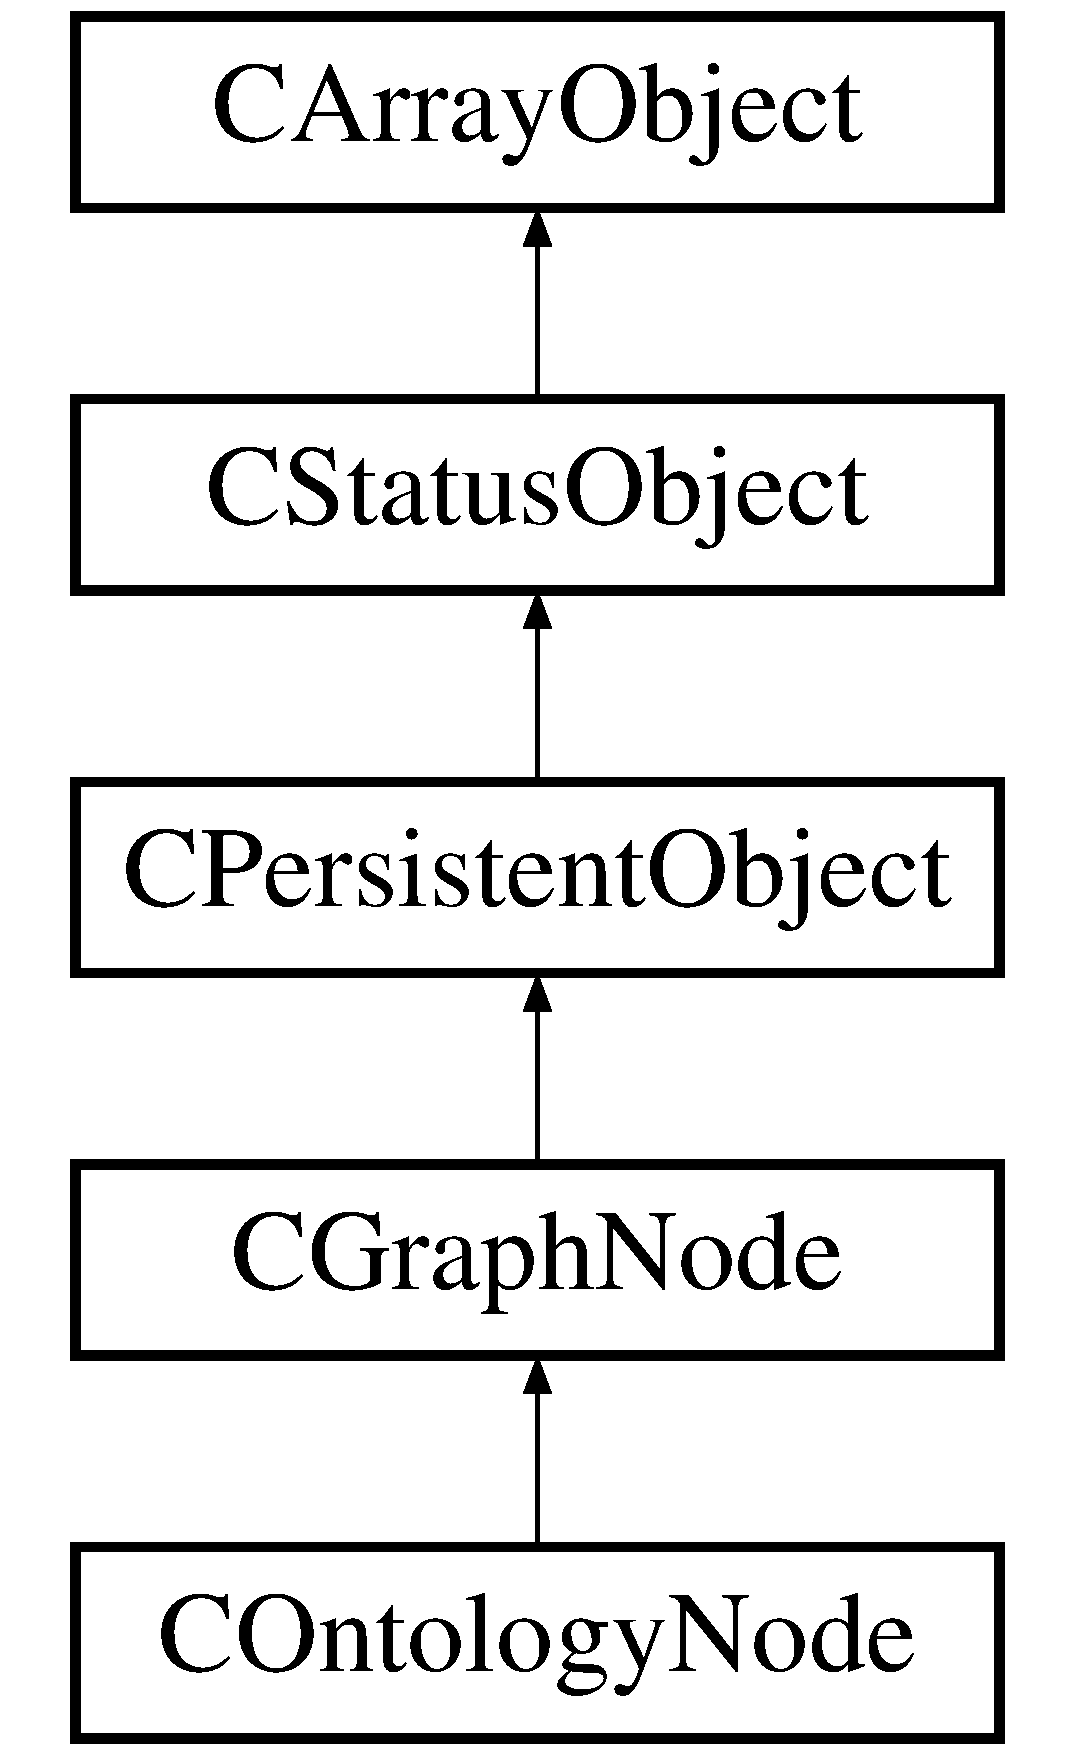
\includegraphics[height=5.000000cm]{class_c_ontology_node}
\end{center}
\end{figure}
\subsection*{Public Member Functions}
\begin{DoxyCompactItemize}
\item 
\hyperlink{class_c_ontology_node_ae074c6f51676b4ef5fc3d7fd1c3149af}{\-\_\-\-\_\-to\-String} ()
\item 
\hyperlink{class_c_ontology_node_a2f294a9c93079f58190cedbdd0c09068}{Term} (\$the\-Value=N\-U\-L\-L, \$get\-Old=F\-A\-L\-S\-E)
\item 
\hyperlink{class_c_ontology_node_a23d374948e7f950726d60163db05c154}{Type} (\$the\-Value=N\-U\-L\-L, \$get\-Old=F\-A\-L\-S\-E)
\item 
\hyperlink{class_c_ontology_node_abfe1cb2e10bb53cf7d500c9860e5cb7a}{Kind} (\$the\-Value=N\-U\-L\-L, \$the\-Operation=N\-U\-L\-L, \$get\-Old=F\-A\-L\-S\-E)
\item 
\hyperlink{class_c_ontology_node_ab96f5c462f470348d014ae0efe43005e}{Domain} (\$the\-Value=N\-U\-L\-L, \$the\-Operation=N\-U\-L\-L, \$get\-Old=F\-A\-L\-S\-E)
\item 
\hyperlink{class_c_ontology_node_a414cd8f920944bed65962492ddb9ce2c}{Category} (\$the\-Value=N\-U\-L\-L, \$the\-Operation=N\-U\-L\-L, \$get\-Old=F\-A\-L\-S\-E)
\item 
\hyperlink{class_c_ontology_node_a80910f44a576ccb643571d24f618d70b}{Relate\-To} (\$the\-Container, \$the\-Predicate, \$the\-Object=N\-U\-L\-L)
\item 
\hyperlink{class_c_ontology_node_a73c05b55f31dc210c549faaf7b914761}{Get\-Related} (\$the\-Container, \$the\-Predicate=N\-U\-L\-L, \$the\-Direction= 'all')
\item 
\hyperlink{class_c_ontology_node_af00ed26a322d8f6c97d07a80e8be980d}{offset\-Exists} (\$the\-Offset)
\item 
\hyperlink{class_c_ontology_node_a73a49b503182510cd7451465ee41c6f2}{offset\-Get} (\$the\-Offset)
\item 
\hyperlink{class_c_ontology_node_aa3702123ca5c04ef0f38a011702df49d}{count} ()
\item 
\hyperlink{class_c_ontology_node_a0172babacb8a6d87eef8d6c76a9aa98f}{get\-Array\-Copy} ()
\end{DoxyCompactItemize}
\subsection*{Protected Member Functions}
\begin{DoxyCompactItemize}
\item 
\hyperlink{class_c_ontology_node_a590c869a08d167ba35d987e450106a2d}{\-\_\-\-Commit} (\&\$the\-Container, \&\$the\-Identifier, \&\$the\-Modifiers)
\item 
\hyperlink{class_c_ontology_node_a7a8304ab0e782d621012edddd8e7da3a}{\-\_\-\-Load} (\&\$the\-Container, \&\$the\-Identifier, \&\$the\-Modifiers)
\item 
\hyperlink{class_c_ontology_node_a8dd4c8bc984a535448618bbbba987a55}{\-\_\-\-Prepare\-Create} (\&\$the\-Container, \&\$the\-Identifier, \&\$the\-Modifiers)
\item 
\hyperlink{class_c_ontology_node_ac8a77d7437a9be4b4aa18626b1a9f95d}{\-\_\-\-Prepare\-Load} (\&\$the\-Container, \&\$the\-Identifier, \&\$the\-Modifiers)
\item 
\hyperlink{class_c_ontology_node_a460df05b73fd4160e7a652ed3b03dd78}{\-\_\-\-Prepare\-Commit} (\&\$the\-Container, \&\$the\-Identifier, \&\$the\-Modifiers)
\item 
\hyperlink{class_c_ontology_node_a3f116a2f1a1047da5187f21e20d3d405}{\-\_\-\-Finish\-Create} (\&\$the\-Container)
\item 
\hyperlink{class_c_ontology_node_a97c5e875641e3bb3da83d32ed8b26ebc}{\-\_\-\-Finish\-Load} (\&\$the\-Container, \&\$the\-Identifier, \&\$the\-Modifiers)
\item 
\hyperlink{class_c_ontology_node_a71d6391728200e6c77a4da829fdced6d}{\-\_\-\-Index\-Terms} (Everyman\textbackslash{}\-Neo4j\textbackslash{}\-Client \$the\-Container)
\item 
\hyperlink{class_c_ontology_node_ae5ca78d7d563ddd125aaffc13fb1d94b}{\-\_\-\-Index\-Nodes} (Everyman\textbackslash{}\-Neo4j\textbackslash{}\-Client \$the\-Container)
\item 
\hyperlink{class_c_ontology_node_ad55eaf2d688301aaa8ce9680640fb9ac}{\-\_\-\-Get\-Node\-Index} (Everyman\textbackslash{}\-Neo4j\textbackslash{}\-Client \$the\-Container, \$the\-Index, \$do\-Clear=F\-A\-L\-S\-E)
\item 
\hyperlink{class_c_ontology_node_ad8be3ea0ae6817b5d902b020885a1919}{\-\_\-\-Manage\-Property} (\$the\-Offset, \$the\-Value=N\-U\-L\-L, \$get\-Old=F\-A\-L\-S\-E)
\item 
\hyperlink{class_c_ontology_node_a0cd827cbc69208b7bdb7c670ed5c3544}{\-\_\-\-Manage\-Property\-Array} (\$the\-Offset, \$the\-Value=N\-U\-L\-L, \$the\-Operation=N\-U\-L\-L, \$get\-Old=F\-A\-L\-S\-E)
\end{DoxyCompactItemize}
\subsection*{Protected Attributes}
\begin{DoxyCompactItemize}
\item 
\hypertarget{class_c_ontology_node_a23aa9d9d9cde004bc251dc98c192652d}{{\bfseries \$m\-Term} = N\-U\-L\-L}\label{class_c_ontology_node_a23aa9d9d9cde004bc251dc98c192652d}

\end{DoxyCompactItemize}


\subsection{Member Function Documentation}
\hypertarget{class_c_ontology_node_ae074c6f51676b4ef5fc3d7fd1c3149af}{\index{C\-Ontology\-Node@{C\-Ontology\-Node}!\-\_\-\-\_\-to\-String@{\-\_\-\-\_\-to\-String}}
\index{\-\_\-\-\_\-to\-String@{\-\_\-\-\_\-to\-String}!COntologyNode@{C\-Ontology\-Node}}
\subsubsection[{\-\_\-\-\_\-to\-String}]{\setlength{\rightskip}{0pt plus 5cm}C\-Ontology\-Node\-::\-\_\-\-\_\-to\-String (
\begin{DoxyParamCaption}
{}
\end{DoxyParamCaption}
)}}\label{class_c_ontology_node_ae074c6f51676b4ef5fc3d7fd1c3149af}
Return object identifier.

In this class we return the \hyperlink{class_c_ontology_node_a2f294a9c93079f58190cedbdd0c09068}{term} \hyperlink{class_c_graph_node_ad830025d2d6650006eb6e737bd4f32c0}{node} \hyperlink{}{property}.

public \begin{DoxyReturn}{Returns}
string
\end{DoxyReturn}
\hyperlink{class_c_graph_node_ad830025d2d6650006eb6e737bd4f32c0}{Node()} 

Reimplemented from \hyperlink{class_c_graph_node_a59905bb321a3fb6a1540a6ffba12f2a0}{C\-Graph\-Node}.

\hypertarget{class_c_ontology_node_a590c869a08d167ba35d987e450106a2d}{\index{C\-Ontology\-Node@{C\-Ontology\-Node}!\-\_\-\-Commit@{\-\_\-\-Commit}}
\index{\-\_\-\-Commit@{\-\_\-\-Commit}!COntologyNode@{C\-Ontology\-Node}}
\subsubsection[{\-\_\-\-Commit}]{\setlength{\rightskip}{0pt plus 5cm}C\-Ontology\-Node\-::\-\_\-\-Commit (
\begin{DoxyParamCaption}
\item[{\&}]{\$the\-Container, }
\item[{\&}]{\$the\-Identifier, }
\item[{\&}]{\$the\-Modifiers}
\end{DoxyParamCaption}
)\hspace{0.3cm}{\ttfamily [protected]}}}\label{class_c_ontology_node_a590c869a08d167ba35d987e450106a2d}
Store object in container.

We \hyperlink{class_c_graph_node_a7af17771eaba24551f8c9a465f391c23}{overload} this method to provide the correct container to the \hyperlink{class_c_graph_node}{parent} \hyperlink{class_c_graph_node_a7af17771eaba24551f8c9a465f391c23}{method}.

We also overload this method to store the node properties into a Mongo collection named \hyperlink{}{k\-C\-O\-L\-L\-\_\-\-N\-O\-D\-E\-S}, the record will be indexed by node I\-D as a 64 bit integer.


\begin{DoxyParams}[1]{Parameters}
reference & {\em \&\$the\-Container} & Object container. \\
\hline
reference & {\em \&\$the\-Identifier} & Object identifier. \\
\hline
reference & {\em \&\$the\-Modifiers} & Commit modifiers.\\
\hline
\end{DoxyParams}
protected \begin{DoxyReturn}{Returns}
mixed
\end{DoxyReturn}
\hyperlink{class_c_graph_node_ad830025d2d6650006eb6e737bd4f32c0}{Node()} 

Reimplemented from \hyperlink{class_c_graph_node_a7af17771eaba24551f8c9a465f391c23}{C\-Graph\-Node}.

\hypertarget{class_c_ontology_node_a3f116a2f1a1047da5187f21e20d3d405}{\index{C\-Ontology\-Node@{C\-Ontology\-Node}!\-\_\-\-Finish\-Create@{\-\_\-\-Finish\-Create}}
\index{\-\_\-\-Finish\-Create@{\-\_\-\-Finish\-Create}!COntologyNode@{C\-Ontology\-Node}}
\subsubsection[{\-\_\-\-Finish\-Create}]{\setlength{\rightskip}{0pt plus 5cm}C\-Ontology\-Node\-::\-\_\-\-Finish\-Create (
\begin{DoxyParamCaption}
\item[{\&}]{\$the\-Container}
\end{DoxyParamCaption}
)\hspace{0.3cm}{\ttfamily [protected]}}}\label{class_c_ontology_node_a3f116a2f1a1047da5187f21e20d3d405}
Normalise after a \hyperlink{class_c_graph_node_a90e49bf5e95ccf3c8644196696154268}{create}.

In this class we initialise the \hyperlink{class_c_ontology_node_a2f294a9c93079f58190cedbdd0c09068}{term} if necessary.


\begin{DoxyParams}[1]{Parameters}
reference & {\em \&\$the\-Container} & Object container.\\
\hline
\end{DoxyParams}
protected 

Reimplemented from \hyperlink{class_c_graph_node_a8a8df45cff2375d0bcbb15342ae3960b}{C\-Graph\-Node}.

\hypertarget{class_c_ontology_node_a97c5e875641e3bb3da83d32ed8b26ebc}{\index{C\-Ontology\-Node@{C\-Ontology\-Node}!\-\_\-\-Finish\-Load@{\-\_\-\-Finish\-Load}}
\index{\-\_\-\-Finish\-Load@{\-\_\-\-Finish\-Load}!COntologyNode@{C\-Ontology\-Node}}
\subsubsection[{\-\_\-\-Finish\-Load}]{\setlength{\rightskip}{0pt plus 5cm}C\-Ontology\-Node\-::\-\_\-\-Finish\-Load (
\begin{DoxyParamCaption}
\item[{\&}]{\$the\-Container, }
\item[{\&}]{\$the\-Identifier, }
\item[{\&}]{\$the\-Modifiers}
\end{DoxyParamCaption}
)\hspace{0.3cm}{\ttfamily [protected]}}}\label{class_c_ontology_node_a97c5e875641e3bb3da83d32ed8b26ebc}
Normalise after a \hyperlink{class_c_ontology_node_a7a8304ab0e782d621012edddd8e7da3a}{load}.

In this class we get the \hyperlink{}{term} reference from the node properties and load it.


\begin{DoxyParams}[1]{Parameters}
reference & {\em \&\$the\-Container} & Object container. \\
\hline
reference & {\em \&\$the\-Identifier} & Object identifier. \\
\hline
reference & {\em \&\$the\-Modifiers} & Create modifiers.\\
\hline
\end{DoxyParams}
protected 

Reimplemented from \hyperlink{class_c_graph_node_a23c2beb0fbed1ab67018dd9d78dee8fa}{C\-Graph\-Node}.

\hypertarget{class_c_ontology_node_ad55eaf2d688301aaa8ce9680640fb9ac}{\index{C\-Ontology\-Node@{C\-Ontology\-Node}!\-\_\-\-Get\-Node\-Index@{\-\_\-\-Get\-Node\-Index}}
\index{\-\_\-\-Get\-Node\-Index@{\-\_\-\-Get\-Node\-Index}!COntologyNode@{C\-Ontology\-Node}}
\subsubsection[{\-\_\-\-Get\-Node\-Index}]{\setlength{\rightskip}{0pt plus 5cm}C\-Ontology\-Node\-::\-\_\-\-Get\-Node\-Index (
\begin{DoxyParamCaption}
\item[{Everyman\textbackslash{}\-Neo4j\textbackslash{}\-Client}]{\$the\-Container, }
\item[{}]{\$the\-Index, }
\item[{}]{\$do\-Clear = {\ttfamily FALSE}}
\end{DoxyParamCaption}
)\hspace{0.3cm}{\ttfamily [protected]}}}\label{class_c_ontology_node_ad55eaf2d688301aaa8ce9680640fb9ac}
Retrieve the node index.

This method can be used to return a node index identified by the provided index tag.


\begin{DoxyParams}[1]{Parameters}
Everyman\textbackslash{}\-Neo4j\textbackslash{}\-Client & {\em \$the\-Container} & Node container. \\
\hline
string & {\em \$the\-Index} & Index tag. \\
\hline
boolean & {\em \$do\-Clear} & T\-R\-U\-E means clear index.\\
\hline
\end{DoxyParams}
protected \begin{DoxyReturn}{Returns}
Everyman 
\end{DoxyReturn}
\hypertarget{class_c_ontology_node_ae5ca78d7d563ddd125aaffc13fb1d94b}{\index{C\-Ontology\-Node@{C\-Ontology\-Node}!\-\_\-\-Index\-Nodes@{\-\_\-\-Index\-Nodes}}
\index{\-\_\-\-Index\-Nodes@{\-\_\-\-Index\-Nodes}!COntologyNode@{C\-Ontology\-Node}}
\subsubsection[{\-\_\-\-Index\-Nodes}]{\setlength{\rightskip}{0pt plus 5cm}C\-Ontology\-Node\-::\-\_\-\-Index\-Nodes (
\begin{DoxyParamCaption}
\item[{Everyman\textbackslash{}\-Neo4j\textbackslash{}\-Client}]{\$the\-Container}
\end{DoxyParamCaption}
)\hspace{0.3cm}{\ttfamily [protected]}}}\label{class_c_ontology_node_ae5ca78d7d563ddd125aaffc13fb1d94b}
Create node property indexes.

This method will save node indexes after the node was \hyperlink{class_c_ontology_node_a590c869a08d167ba35d987e450106a2d}{committed}, there are two main indexes for node properties\-:


\begin{DoxyItemize}
\item {\itshape \hyperlink{}{k\-I\-N\-D\-E\-X\-\_\-\-N\-O\-D\-E\-\_\-\-N\-O\-D\-E}}\-: This index (Node\-Index) links the node to its properties through the following keys\-: 
\begin{DoxyItemize}
\item {\itshape \hyperlink{}{k\-T\-A\-G\-\_\-\-T\-Y\-P\-E}}\-: This key links the current node to its \hyperlink{class_c_ontology_node_a23d374948e7f950726d60163db05c154}{type}, which may either be inherited from its \hyperlink{class_c_ontology_node_a2f294a9c93079f58190cedbdd0c09068}{term} or have been \hyperlink{class_c_ontology_node_a23d374948e7f950726d60163db05c154}{explicitly} set. 
\item {\itshape \hyperlink{}{k\-T\-A\-G\-\_\-\-K\-I\-N\-D}}\-: This key links the current node to its \hyperlink{class_c_ontology_node_abfe1cb2e10bb53cf7d500c9860e5cb7a}{kinds}, which may either be inherited from its \hyperlink{class_c_ontology_node_a2f294a9c93079f58190cedbdd0c09068}{term} or have been \hyperlink{class_c_ontology_node_abfe1cb2e10bb53cf7d500c9860e5cb7a}{explicitly} set. 
\item {\itshape \hyperlink{}{k\-T\-A\-G\-\_\-\-D\-O\-M\-A\-I\-N}}\-: This key links the current node to its \hyperlink{class_c_ontology_node_ab96f5c462f470348d014ae0efe43005e}{domains}, which may either be inherited from its \hyperlink{class_c_ontology_node_a2f294a9c93079f58190cedbdd0c09068}{term} or have been \hyperlink{class_c_ontology_node_ab96f5c462f470348d014ae0efe43005e}{explicitly} set. 
\item {\itshape \hyperlink{}{k\-T\-A\-G\-\_\-\-C\-A\-T\-E\-G\-O\-R\-Y}}\-: This key links the current node to its \hyperlink{class_c_ontology_node_a414cd8f920944bed65962492ddb9ce2c}{categories}, which may either be inherited from its \hyperlink{class_c_ontology_node_a414cd8f920944bed65962492ddb9ce2c}{term} or have been \hyperlink{class_c_ontology_node_a414cd8f920944bed65962492ddb9ce2c}{explicitly} set. 
\end{DoxyItemize}
\end{DoxyItemize}


\begin{DoxyParams}[1]{Parameters}
Everyman\textbackslash{}\-Neo4j\textbackslash{}\-Client & {\em \$the\-Container} & Node container.\\
\hline
\end{DoxyParams}
protected \hypertarget{class_c_ontology_node_a71d6391728200e6c77a4da829fdced6d}{\index{C\-Ontology\-Node@{C\-Ontology\-Node}!\-\_\-\-Index\-Terms@{\-\_\-\-Index\-Terms}}
\index{\-\_\-\-Index\-Terms@{\-\_\-\-Index\-Terms}!COntologyNode@{C\-Ontology\-Node}}
\subsubsection[{\-\_\-\-Index\-Terms}]{\setlength{\rightskip}{0pt plus 5cm}C\-Ontology\-Node\-::\-\_\-\-Index\-Terms (
\begin{DoxyParamCaption}
\item[{Everyman\textbackslash{}\-Neo4j\textbackslash{}\-Client}]{\$the\-Container}
\end{DoxyParamCaption}
)\hspace{0.3cm}{\ttfamily [protected]}}}\label{class_c_ontology_node_a71d6391728200e6c77a4da829fdced6d}
Create node/term indexes.

This method will save node indexes after the node was \hyperlink{class_c_ontology_node_a590c869a08d167ba35d987e450106a2d}{committed}, there are two main indexes for nodes\-:


\begin{DoxyItemize}
\item {\itshape \hyperlink{}{k\-I\-N\-D\-E\-X\-\_\-\-N\-O\-D\-E\-\_\-\-T\-E\-R\-M}}\-: This index (Node\-Index) links the node to its \hyperlink{class_c_ontology_node_a2f294a9c93079f58190cedbdd0c09068}{term} through the following keys\-: 
\begin{DoxyItemize}
\item {\itshape \hyperlink{}{k\-T\-A\-G\-\_\-\-T\-E\-R\-M}}\-: This key represents the \hyperlink{class_c_ontology_node_a2f294a9c93079f58190cedbdd0c09068}{term} \hyperlink{}{identifier}. 
\item {\itshape \hyperlink{}{k\-T\-A\-G\-\_\-\-N\-A\-M\-E}}\-: This key represents the \hyperlink{class_c_ontology_node_a2f294a9c93079f58190cedbdd0c09068}{term} \hyperlink{}{names} in all languages. 
\end{DoxyItemize}
\end{DoxyItemize}


\begin{DoxyParams}[1]{Parameters}
Everyman\textbackslash{}\-Neo4j\textbackslash{}\-Client & {\em \$the\-Container} & Node container.\\
\hline
\end{DoxyParams}
protected \hypertarget{class_c_ontology_node_a7a8304ab0e782d621012edddd8e7da3a}{\index{C\-Ontology\-Node@{C\-Ontology\-Node}!\-\_\-\-Load@{\-\_\-\-Load}}
\index{\-\_\-\-Load@{\-\_\-\-Load}!COntologyNode@{C\-Ontology\-Node}}
\subsubsection[{\-\_\-\-Load}]{\setlength{\rightskip}{0pt plus 5cm}C\-Ontology\-Node\-::\-\_\-\-Load (
\begin{DoxyParamCaption}
\item[{\&}]{\$the\-Container, }
\item[{\&}]{\$the\-Identifier, }
\item[{\&}]{\$the\-Modifiers}
\end{DoxyParamCaption}
)\hspace{0.3cm}{\ttfamily [protected]}}}\label{class_c_ontology_node_a7a8304ab0e782d621012edddd8e7da3a}
Find object.

In this class we try to load the node.


\begin{DoxyParams}[1]{Parameters}
reference & {\em \&\$the\-Container} & Object container. \\
\hline
reference & {\em \&\$the\-Identifier} & Object identifier. \\
\hline
reference & {\em \&\$the\-Modifiers} & Create options.\\
\hline
\end{DoxyParams}
protected \begin{DoxyReturn}{Returns}
mixed 
\end{DoxyReturn}


Reimplemented from \hyperlink{class_c_graph_node_a60c57e754245042fe04dad8fb63a5fec}{C\-Graph\-Node}.

\hypertarget{class_c_ontology_node_ad8be3ea0ae6817b5d902b020885a1919}{\index{C\-Ontology\-Node@{C\-Ontology\-Node}!\-\_\-\-Manage\-Property@{\-\_\-\-Manage\-Property}}
\index{\-\_\-\-Manage\-Property@{\-\_\-\-Manage\-Property}!COntologyNode@{C\-Ontology\-Node}}
\subsubsection[{\-\_\-\-Manage\-Property}]{\setlength{\rightskip}{0pt plus 5cm}C\-Ontology\-Node\-::\-\_\-\-Manage\-Property (
\begin{DoxyParamCaption}
\item[{}]{\$the\-Offset, }
\item[{}]{\$the\-Value = {\ttfamily NULL}, }
\item[{}]{\$get\-Old = {\ttfamily FALSE}}
\end{DoxyParamCaption}
)\hspace{0.3cm}{\ttfamily [protected]}}}\label{class_c_ontology_node_ad8be3ea0ae6817b5d902b020885a1919}
Manage scalar property.

This method will set, retrieve and delete scalar properties, it accepts the following parameters\-:


\begin{DoxyItemize}
\item {\bfseries \$the\-Offset}\-: The property offset to manage. 
\item {\bfseries \$the\-Value}\-: The property value or operation\-: 
\begin{DoxyItemize}
\item {\itshape N\-U\-L\-L}\-: Return the property current value. 
\item {\itshape F\-A\-L\-S\-E}\-: Delete the property. 
\item {\itshape other}\-: Any other type represents the new property value. 
\end{DoxyItemize}
\item {\bfseries \$get\-Old}\-: Determines what the method will return\-: 
\begin{DoxyItemize}
\item {\itshape T\-R\-U\-E}\-: Return the value of the property {\itshape before} it was eventually modified. 
\item {\itshape F\-A\-L\-S\-E}\-: Return the value of the property {\itshape after} it was eventually modified. 
\end{DoxyItemize}
\end{DoxyItemize}

Note that if the current object does no yet have a \hyperlink{class_c_graph_node_ad830025d2d6650006eb6e737bd4f32c0}{node} reference, the method will raise an exception.


\begin{DoxyParams}[1]{Parameters}
string & {\em \$the\-Offset} & Property key. \\
\hline
mixed & {\em \$the\-Value} & Value or operation. \\
\hline
boolean & {\em \$get\-Old} & T\-R\-U\-E get old value.\\
\hline
\end{DoxyParams}
protected \begin{DoxyReturn}{Returns}
mixed
\end{DoxyReturn}

\begin{DoxyExceptions}{Exceptions}
{\em \{@link} & \hyperlink{class_c_exception}{C\-Exception} \hyperlink{class_c_exception}{C\-Exception}\}\\
\hline
\end{DoxyExceptions}
\hyperlink{class_c_graph_node_ad830025d2d6650006eb6e737bd4f32c0}{Node()}  \hyperlink{class_c_status_object_a19c4ac94dfe26476e780d77b99744d43}{\-\_\-\-Is\-Dirty()} \hypertarget{class_c_ontology_node_a0cd827cbc69208b7bdb7c670ed5c3544}{\index{C\-Ontology\-Node@{C\-Ontology\-Node}!\-\_\-\-Manage\-Property\-Array@{\-\_\-\-Manage\-Property\-Array}}
\index{\-\_\-\-Manage\-Property\-Array@{\-\_\-\-Manage\-Property\-Array}!COntologyNode@{C\-Ontology\-Node}}
\subsubsection[{\-\_\-\-Manage\-Property\-Array}]{\setlength{\rightskip}{0pt plus 5cm}C\-Ontology\-Node\-::\-\_\-\-Manage\-Property\-Array (
\begin{DoxyParamCaption}
\item[{}]{\$the\-Offset, }
\item[{}]{\$the\-Value = {\ttfamily NULL}, }
\item[{}]{\$the\-Operation = {\ttfamily NULL}, }
\item[{}]{\$get\-Old = {\ttfamily FALSE}}
\end{DoxyParamCaption}
)\hspace{0.3cm}{\ttfamily [protected]}}}\label{class_c_ontology_node_a0cd827cbc69208b7bdb7c670ed5c3544}
Manage scalar property.

This method will set, retrieve and delete array element properties, it accepts the following parameters\-:


\begin{DoxyItemize}
\item {\bfseries \$the\-Offset}\-: The property offset to manage. 
\item {\bfseries \$the\-Value}\-: This parameter represents either the value to add, or the index of the element to operate on\-: 
\begin{DoxyItemize}
\item {\itshape N\-U\-L\-L}\-: This value indicates that we want to operate on all elements, which means that we are retrieving the full list or deleting it. 
\item {\itshape array}\-: This value indicates that we want to replace the whole list, this will only be tested if the next parameter evaluates to {\itshape T\-R\-U\-E}. 
\item {\itshape other}\-: Any other type represents either the new value to be added or the index to the value to be returned or deleted. {\itshape It must be possible to cast this value to a string, this is what will be used to compare elements}. 
\end{DoxyItemize}
\item {\bfseries \$the\-Operation}\-: This parameter represents the operation to be performed, it will be evaluated as a boolean and its scope depends on the value of the previous parameter\-: 
\begin{DoxyItemize}
\item {\itshape N\-U\-L\-L}\-: Return the element or list. 
\item {\itshape F\-A\-L\-S\-E}\-: Delete the element or list. 
\item {\itshape T\-R\-U\-E}\-: Add the element or list. Note that with this value, if you provide {\itshape N\-U\-L\-L} in the previous parameter, it will be equivalent to deleting the whole list. 
\end{DoxyItemize}
\item {\bfseries \$get\-Old}\-: Determines what the method will return\-: 
\begin{DoxyItemize}
\item {\itshape T\-R\-U\-E}\-: Return the element or list {\itshape before} it was eventually modified. 
\item {\itshape F\-A\-L\-S\-E}\-: Return the element or list {\itshape after} it was eventually modified. 
\end{DoxyItemize}
\end{DoxyItemize}


\begin{DoxyParams}[1]{Parameters}
string & {\em \$the\-Offset} & Property key. \\
\hline
mixed & {\em \$the\-Value} & Value or index. \\
\hline
mixed & {\em \$the\-Operation} & Operation. \\
\hline
boolean & {\em \$get\-Old} & T\-R\-U\-E get old value.\\
\hline
\end{DoxyParams}
\begin{DoxyReturn}{Returns}
mixed
\end{DoxyReturn}

\begin{DoxyExceptions}{Exceptions}
{\em \{@link} & \hyperlink{class_c_exception}{C\-Exception} \hyperlink{class_c_exception}{C\-Exception}\}\\
\hline
\end{DoxyExceptions}
\hyperlink{class_c_graph_node_ad830025d2d6650006eb6e737bd4f32c0}{Node()}  \hyperlink{class_c_status_object_a19c4ac94dfe26476e780d77b99744d43}{\-\_\-\-Is\-Dirty()} \hypertarget{class_c_ontology_node_a460df05b73fd4160e7a652ed3b03dd78}{\index{C\-Ontology\-Node@{C\-Ontology\-Node}!\-\_\-\-Prepare\-Commit@{\-\_\-\-Prepare\-Commit}}
\index{\-\_\-\-Prepare\-Commit@{\-\_\-\-Prepare\-Commit}!COntologyNode@{C\-Ontology\-Node}}
\subsubsection[{\-\_\-\-Prepare\-Commit}]{\setlength{\rightskip}{0pt plus 5cm}C\-Ontology\-Node\-::\-\_\-\-Prepare\-Commit (
\begin{DoxyParamCaption}
\item[{\&}]{\$the\-Container, }
\item[{\&}]{\$the\-Identifier, }
\item[{\&}]{\$the\-Modifiers}
\end{DoxyParamCaption}
)\hspace{0.3cm}{\ttfamily [protected]}}}\label{class_c_ontology_node_a460df05b73fd4160e7a652ed3b03dd78}
Normalise before a store.

In this class we check if the provided container is supported and we set the \hyperlink{}{term} property in the node and \hyperlink{class_c_persistent_object_a88b1f2b11d3d60e0b3d33d8b0649b68a}{commit} the \hyperlink{class_c_ontology_node_a2f294a9c93079f58190cedbdd0c09068}{term}.

We also copy the \hyperlink{class_c_coded_unit_object_aafe9f12551f9f183c21a9865f0e9c670}{kind}, \hyperlink{class_c_term_a2527808f249d6880b327e08a9cce0911}{domain}, \hyperlink{class_c_term_a6ab25cb91c1a6de266e58ccad919ffba}{category} and \hyperlink{class_c_ontology_term_afd46ef8241b696e99cf7b5e1334914b7}{type} elements, if not yet present, from the \hyperlink{class_c_ontology_node_a2f294a9c93079f58190cedbdd0c09068}{term} to the current node.


\begin{DoxyParams}[1]{Parameters}
reference & {\em \&\$the\-Container} & Object container. \\
\hline
reference & {\em \&\$the\-Identifier} & Object identifier. \\
\hline
reference & {\em \&\$the\-Modifiers} & Commit modifiers.\\
\hline
\end{DoxyParams}
protected


\begin{DoxyExceptions}{Exceptions}
{\em \{@link} & \hyperlink{class_c_exception}{C\-Exception} \hyperlink{class_c_exception}{C\-Exception}\} \\
\hline
\end{DoxyExceptions}


Reimplemented from \hyperlink{class_c_graph_node_ad55d35f1ac947bae32fe8019daf05112}{C\-Graph\-Node}.

\hypertarget{class_c_ontology_node_a8dd4c8bc984a535448618bbbba987a55}{\index{C\-Ontology\-Node@{C\-Ontology\-Node}!\-\_\-\-Prepare\-Create@{\-\_\-\-Prepare\-Create}}
\index{\-\_\-\-Prepare\-Create@{\-\_\-\-Prepare\-Create}!COntologyNode@{C\-Ontology\-Node}}
\subsubsection[{\-\_\-\-Prepare\-Create}]{\setlength{\rightskip}{0pt plus 5cm}C\-Ontology\-Node\-::\-\_\-\-Prepare\-Create (
\begin{DoxyParamCaption}
\item[{\&}]{\$the\-Container, }
\item[{\&}]{\$the\-Identifier, }
\item[{\&}]{\$the\-Modifiers}
\end{DoxyParamCaption}
)\hspace{0.3cm}{\ttfamily [protected]}}}\label{class_c_ontology_node_a8dd4c8bc984a535448618bbbba987a55}
Normalise parameters of a create.

In this class we first check whether the container has the following structure\-:


\begin{DoxyItemize}
\item {\itshape \hyperlink{}{k\-T\-A\-G\-\_\-\-N\-O\-D\-E}}\-: This element should hold the nodes container, it must be a Everyman instance. 
\item {\itshape \hyperlink{}{k\-T\-A\-G\-\_\-\-T\-E\-R\-M}}\-: This element should hold the terms container, it must be a \hyperlink{class_c_ontology_term_object}{C\-Ontology\-Term\-Object} instance. 
\end{DoxyItemize}

We then call the \hyperlink{class_c_graph_node}{parent} \hyperlink{class_c_graph_node_a500c59ddfbec7fedf8598ee5d886de67}{method} and check if the container was replaced with the content\-: in that case we try to load the related \hyperlink{class_c_ontology_node_a2f294a9c93079f58190cedbdd0c09068}{term}.


\begin{DoxyParams}[1]{Parameters}
reference & {\em \&\$the\-Container} & Object container. \\
\hline
reference & {\em \&\$the\-Identifier} & Object identifier. \\
\hline
reference & {\em \&\$the\-Modifiers} & Create modifiers.\\
\hline
\end{DoxyParams}
protected

\hyperlink{class_c_persistent_object_aa8dc7db66e2af3d28c2035161a2aabf9}{\-\_\-\-Is\-Encoded()}

\begin{DoxySeeAlso}{See also}
k\-F\-L\-A\-G\-\_\-\-S\-T\-A\-T\-E\-\_\-\-E\-N\-C\-O\-D\-E\-D 
\end{DoxySeeAlso}


Reimplemented from \hyperlink{class_c_graph_node_a500c59ddfbec7fedf8598ee5d886de67}{C\-Graph\-Node}.

\hypertarget{class_c_ontology_node_ac8a77d7437a9be4b4aa18626b1a9f95d}{\index{C\-Ontology\-Node@{C\-Ontology\-Node}!\-\_\-\-Prepare\-Load@{\-\_\-\-Prepare\-Load}}
\index{\-\_\-\-Prepare\-Load@{\-\_\-\-Prepare\-Load}!COntologyNode@{C\-Ontology\-Node}}
\subsubsection[{\-\_\-\-Prepare\-Load}]{\setlength{\rightskip}{0pt plus 5cm}C\-Ontology\-Node\-::\-\_\-\-Prepare\-Load (
\begin{DoxyParamCaption}
\item[{\&}]{\$the\-Container, }
\item[{\&}]{\$the\-Identifier, }
\item[{\&}]{\$the\-Modifiers}
\end{DoxyParamCaption}
)\hspace{0.3cm}{\ttfamily [protected]}}}\label{class_c_ontology_node_ac8a77d7437a9be4b4aa18626b1a9f95d}
Normalise parameters of a find.

In this class we check if the provided container is supported., terms require a container instance derived from \hyperlink{class_c_container}{C\-Container}.


\begin{DoxyParams}[1]{Parameters}
reference & {\em \&\$the\-Container} & Object container. \\
\hline
reference & {\em \&\$the\-Identifier} & Object identifier. \\
\hline
reference & {\em \&\$the\-Modifiers} & Create modifiers.\\
\hline
\end{DoxyParams}
protected


\begin{DoxyExceptions}{Exceptions}
{\em \{@link} & \hyperlink{class_c_exception}{C\-Exception} \hyperlink{class_c_exception}{C\-Exception}\} \\
\hline
\end{DoxyExceptions}


Reimplemented from \hyperlink{class_c_graph_node_af9f27bcc601672903af33f33d62e7ebf}{C\-Graph\-Node}.

\hypertarget{class_c_ontology_node_a414cd8f920944bed65962492ddb9ce2c}{\index{C\-Ontology\-Node@{C\-Ontology\-Node}!Category@{Category}}
\index{Category@{Category}!COntologyNode@{C\-Ontology\-Node}}
\subsubsection[{Category}]{\setlength{\rightskip}{0pt plus 5cm}C\-Ontology\-Node\-::\-Category (
\begin{DoxyParamCaption}
\item[{}]{\$the\-Value = {\ttfamily NULL}, }
\item[{}]{\$the\-Operation = {\ttfamily NULL}, }
\item[{}]{\$get\-Old = {\ttfamily FALSE}}
\end{DoxyParamCaption}
)}}\label{class_c_ontology_node_a414cd8f920944bed65962492ddb9ce2c}
Manage node kind.

This method can be used to manage the node \hyperlink{}{categories}, in general it reflects the \hyperlink{class_c_ontology_node_a2f294a9c93079f58190cedbdd0c09068}{term} \hyperlink{class_c_term_a6ab25cb91c1a6de266e58ccad919ffba}{categories}.

For a more thorough reference of how this method works, please consult the \hyperlink{class_c_ontology_node_a0cd827cbc69208b7bdb7c670ed5c3544}{\-\_\-\-Manage\-Property\-Array} method, in which the first parameter will be the constant \hyperlink{}{k\-T\-A\-G\-\_\-\-C\-A\-T\-E\-G\-O\-R\-Y}.

The method will also set the \hyperlink{class_c_status_object_a19c4ac94dfe26476e780d77b99744d43}{dirty} \hyperlink{}{status}.


\begin{DoxyParams}[1]{Parameters}
mixed & {\em \$the\-Value} & Term or operation. \\
\hline
boolean & {\em \$get\-Old} & T\-R\-U\-E get old value.\\
\hline
\end{DoxyParams}
public \begin{DoxyReturn}{Returns}
string
\end{DoxyReturn}
\hyperlink{class_c_ontology_node_a0cd827cbc69208b7bdb7c670ed5c3544}{\-\_\-\-Manage\-Property\-Array()}

\begin{DoxySeeAlso}{See also}
k\-T\-A\-G\-\_\-\-C\-A\-T\-E\-G\-O\-R\-Y 
\end{DoxySeeAlso}
\hypertarget{class_c_ontology_node_aa3702123ca5c04ef0f38a011702df49d}{\index{C\-Ontology\-Node@{C\-Ontology\-Node}!count@{count}}
\index{count@{count}!COntologyNode@{C\-Ontology\-Node}}
\subsubsection[{count}]{\setlength{\rightskip}{0pt plus 5cm}C\-Ontology\-Node\-::count (
\begin{DoxyParamCaption}
{}
\end{DoxyParamCaption}
)}}\label{class_c_ontology_node_aa3702123ca5c04ef0f38a011702df49d}
Count number of elements.

We overload this method to wrap the internal array over the node properties.

Note that if the node exists the method will return an integer, if not, it will return {\itshape N\-U\-L\-L}.

public \begin{DoxyReturn}{Returns}
mixed 
\end{DoxyReturn}


Reimplemented from \hyperlink{class_c_graph_node_a31fffee579cebb625adbee4e4f53bb48}{C\-Graph\-Node}.

\hypertarget{class_c_ontology_node_ab96f5c462f470348d014ae0efe43005e}{\index{C\-Ontology\-Node@{C\-Ontology\-Node}!Domain@{Domain}}
\index{Domain@{Domain}!COntologyNode@{C\-Ontology\-Node}}
\subsubsection[{Domain}]{\setlength{\rightskip}{0pt plus 5cm}C\-Ontology\-Node\-::\-Domain (
\begin{DoxyParamCaption}
\item[{}]{\$the\-Value = {\ttfamily NULL}, }
\item[{}]{\$the\-Operation = {\ttfamily NULL}, }
\item[{}]{\$get\-Old = {\ttfamily FALSE}}
\end{DoxyParamCaption}
)}}\label{class_c_ontology_node_ab96f5c462f470348d014ae0efe43005e}
Manage node kind.

This method can be used to manage the node \hyperlink{}{domains}, in general it reflects the \hyperlink{class_c_ontology_node_a2f294a9c93079f58190cedbdd0c09068}{term} \hyperlink{class_c_term_a2527808f249d6880b327e08a9cce0911}{domains}.

For a more thorough reference of how this method works, please consult the \hyperlink{class_c_ontology_node_a0cd827cbc69208b7bdb7c670ed5c3544}{\-\_\-\-Manage\-Property\-Array} method, in which the first parameter will be the constant \hyperlink{}{k\-T\-A\-G\-\_\-\-D\-O\-M\-A\-I\-N}.

The method will also set the \hyperlink{class_c_status_object_a19c4ac94dfe26476e780d77b99744d43}{dirty} \hyperlink{}{status}.


\begin{DoxyParams}[1]{Parameters}
mixed & {\em \$the\-Value} & Term or operation. \\
\hline
boolean & {\em \$get\-Old} & T\-R\-U\-E get old value.\\
\hline
\end{DoxyParams}
public \begin{DoxyReturn}{Returns}
string
\end{DoxyReturn}
\hyperlink{class_c_ontology_node_a0cd827cbc69208b7bdb7c670ed5c3544}{\-\_\-\-Manage\-Property\-Array()}

\begin{DoxySeeAlso}{See also}
k\-T\-A\-G\-\_\-\-D\-O\-M\-A\-I\-N 
\end{DoxySeeAlso}
\hypertarget{class_c_ontology_node_a0172babacb8a6d87eef8d6c76a9aa98f}{\index{C\-Ontology\-Node@{C\-Ontology\-Node}!get\-Array\-Copy@{get\-Array\-Copy}}
\index{get\-Array\-Copy@{get\-Array\-Copy}!COntologyNode@{C\-Ontology\-Node}}
\subsubsection[{get\-Array\-Copy}]{\setlength{\rightskip}{0pt plus 5cm}C\-Ontology\-Node\-::get\-Array\-Copy (
\begin{DoxyParamCaption}
{}
\end{DoxyParamCaption}
)}}\label{class_c_ontology_node_a0172babacb8a6d87eef8d6c76a9aa98f}
Create a copy of the array.

We overload this method to wrap the internal array over the node properties.

Note that if the node exists the method will return an array, if not, it will return an empty array.

public \begin{DoxyReturn}{Returns}
mixed 
\end{DoxyReturn}


Reimplemented from \hyperlink{class_c_graph_node_a8a47a42830cc926da243f60838a08d7f}{C\-Graph\-Node}.

\hypertarget{class_c_ontology_node_a73c05b55f31dc210c549faaf7b914761}{\index{C\-Ontology\-Node@{C\-Ontology\-Node}!Get\-Related@{Get\-Related}}
\index{Get\-Related@{Get\-Related}!COntologyNode@{C\-Ontology\-Node}}
\subsubsection[{Get\-Related}]{\setlength{\rightskip}{0pt plus 5cm}C\-Ontology\-Node\-::\-Get\-Related (
\begin{DoxyParamCaption}
\item[{}]{\$the\-Container, }
\item[{}]{\$the\-Predicate = {\ttfamily NULL}, }
\item[{}]{\$the\-Direction = {\ttfamily 'all'}}
\end{DoxyParamCaption}
)}}\label{class_c_ontology_node_a73c05b55f31dc210c549faaf7b914761}
Return related \hyperlink{class_c_ontology_edge}{edges}.

This method will return all nodes that are related to the current one in an array of \hyperlink{class_c_ontology_edge}{edge} nodes whose elements are structured as follows\-:


\begin{DoxyItemize}
\item {\itshape Key}\-: The edge I\-D. 
\item {\itshape Value}\-: The edge \hyperlink{class_c_ontology_edge}{object}. 
\end{DoxyItemize}

The method accepts the following parameters\-:


\begin{DoxyItemize}
\item {\bfseries \$the\-Container}\-: The graph and term containers as an array\-: 
\begin{DoxyItemize}
\item {\itshape \hyperlink{}{k\-T\-A\-G\-\_\-\-N\-O\-D\-E}}\-: This element should hold the nodes container, it must be a Everyman instance. 
\item {\itshape \hyperlink{}{k\-T\-A\-G\-\_\-\-T\-E\-R\-M}}\-: This element should hold the terms container, it must be a \hyperlink{class_c_container}{C\-Container} instance. 
\end{DoxyItemize}
\item {\bfseries \$the\-Predicate}\-: The predicate terms as an array of the following types\-: 
\begin{DoxyItemize}
\item {\itshape \hyperlink{class_c_ontology_node}{C\-Ontology\-Node}}\-: The node \hyperlink{class_c_ontology_node_a2f294a9c93079f58190cedbdd0c09068}{term} \hyperlink{}{global} \hyperlink{class_c_ontology_term_object_ab1a4d21bb56a8a6cf3f77f595d776267}{identifier}. 
\item {\itshape \hyperlink{class_c_ontology_term}{C\-Ontology\-Term}}\-: The term \hyperlink{}{global} identifier will be used as the \hyperlink{class_c_ontology_edge}{node} \hyperlink{class_c_graph_edge_a584c0263fd773ffb764385a51d36caf2}{type}. 
\item {\itshape Everyman}\-: The relationship's type will be used as the predicate, all other elements of the provided edge node will be ignored. 
\item {\itshape string}\-: Any other type will be converted to string and will be used as the \hyperlink{class_c_ontology_edge}{node} \hyperlink{class_c_graph_edge_a584c0263fd773ffb764385a51d36caf2}{type}. 
\end{DoxyItemize}
\item {\bfseries \$the\-Direction}\-: The direction of the relation\-: 
\begin{DoxyItemize}
\item {\itshape out}\-: Outgoing relations, the current node is the subject. 
\item {\itshape in}\-: Incoming relations, the current node is the object. 
\item {\itshape all}\-: Incoming and outgoing relations (default), the current node is the object or the subject. 
\end{DoxyItemize}
\end{DoxyItemize}


\begin{DoxyParams}[1]{Parameters}
reference & {\em \$the\-Container} & Object container. \\
\hline
mixed & {\em \$the\-Predicate} & Predicate. \\
\hline
string & {\em \$the\-Direction} & Relation direction.\\
\hline
\end{DoxyParams}
protected \begin{DoxyReturn}{Returns}
array
\end{DoxyReturn}

\begin{DoxyExceptions}{Exceptions}
{\em \{@link} & \hyperlink{class_c_exception}{C\-Exception} \hyperlink{class_c_exception}{C\-Exception}\} \\
\hline
\end{DoxyExceptions}
\hypertarget{class_c_ontology_node_abfe1cb2e10bb53cf7d500c9860e5cb7a}{\index{C\-Ontology\-Node@{C\-Ontology\-Node}!Kind@{Kind}}
\index{Kind@{Kind}!COntologyNode@{C\-Ontology\-Node}}
\subsubsection[{Kind}]{\setlength{\rightskip}{0pt plus 5cm}C\-Ontology\-Node\-::\-Kind (
\begin{DoxyParamCaption}
\item[{}]{\$the\-Value = {\ttfamily NULL}, }
\item[{}]{\$the\-Operation = {\ttfamily NULL}, }
\item[{}]{\$get\-Old = {\ttfamily FALSE}}
\end{DoxyParamCaption}
)}}\label{class_c_ontology_node_abfe1cb2e10bb53cf7d500c9860e5cb7a}
Manage node kind.

This method can be used to manage the node \hyperlink{}{kinds}, in general it reflects the \hyperlink{class_c_ontology_node_a2f294a9c93079f58190cedbdd0c09068}{term} \hyperlink{class_c_coded_unit_object_aafe9f12551f9f183c21a9865f0e9c670}{kinds}.

For a more thorough reference of how this method works, please consult the \hyperlink{class_c_ontology_node_a0cd827cbc69208b7bdb7c670ed5c3544}{\-\_\-\-Manage\-Property\-Array} method, in which the first parameter will be the constant \hyperlink{}{k\-T\-A\-G\-\_\-\-K\-I\-N\-D}.

The method will also set the \hyperlink{class_c_status_object_a19c4ac94dfe26476e780d77b99744d43}{dirty} \hyperlink{}{status}.


\begin{DoxyParams}[1]{Parameters}
mixed & {\em \$the\-Value} & Value or index. \\
\hline
mixed & {\em \$the\-Operation} & Operation. \\
\hline
boolean & {\em \$get\-Old} & T\-R\-U\-E get old value.\\
\hline
\end{DoxyParams}
public \begin{DoxyReturn}{Returns}
string
\end{DoxyReturn}
\hyperlink{class_c_ontology_node_a0cd827cbc69208b7bdb7c670ed5c3544}{\-\_\-\-Manage\-Property\-Array()}

\begin{DoxySeeAlso}{See also}
k\-T\-A\-G\-\_\-\-K\-I\-N\-D 
\end{DoxySeeAlso}
\hypertarget{class_c_ontology_node_af00ed26a322d8f6c97d07a80e8be980d}{\index{C\-Ontology\-Node@{C\-Ontology\-Node}!offset\-Exists@{offset\-Exists}}
\index{offset\-Exists@{offset\-Exists}!COntologyNode@{C\-Ontology\-Node}}
\subsubsection[{offset\-Exists}]{\setlength{\rightskip}{0pt plus 5cm}C\-Ontology\-Node\-::offset\-Exists (
\begin{DoxyParamCaption}
\item[{}]{\$the\-Offset}
\end{DoxyParamCaption}
)}}\label{class_c_ontology_node_af00ed26a322d8f6c97d07a80e8be980d}
Check whether a given offset exists.

We overload this method to wrap the internal array over the node properties.


\begin{DoxyParams}[1]{Parameters}
string & {\em \$the\-Offset} & Offset.\\
\hline
\end{DoxyParams}
public \begin{DoxyReturn}{Returns}
boolean 
\end{DoxyReturn}


Reimplemented from \hyperlink{class_c_graph_node_a8c567e73a79cddc0e3582b3bd766d980}{C\-Graph\-Node}.

\hypertarget{class_c_ontology_node_a73a49b503182510cd7451465ee41c6f2}{\index{C\-Ontology\-Node@{C\-Ontology\-Node}!offset\-Get@{offset\-Get}}
\index{offset\-Get@{offset\-Get}!COntologyNode@{C\-Ontology\-Node}}
\subsubsection[{offset\-Get}]{\setlength{\rightskip}{0pt plus 5cm}C\-Ontology\-Node\-::offset\-Get (
\begin{DoxyParamCaption}
\item[{}]{\$the\-Offset}
\end{DoxyParamCaption}
)}}\label{class_c_ontology_node_a73a49b503182510cd7451465ee41c6f2}
Return a value at a given offset.

We overload this method to wrap the internal array over the node properties.

In this class no offset may have a {\itshape N\-U\-L\-L} value, if this method returns a {\itshape N\-U\-L\-L} value, it means that the offset doesn't exist.


\begin{DoxyParams}[1]{Parameters}
string & {\em \$the\-Offset} & Offset.\\
\hline
\end{DoxyParams}
public \begin{DoxyReturn}{Returns}
mixed 
\end{DoxyReturn}


Reimplemented from \hyperlink{class_c_graph_node_a0a00e251025e4f7b10beae2248f03d77}{C\-Graph\-Node}.

\hypertarget{class_c_ontology_node_a80910f44a576ccb643571d24f618d70b}{\index{C\-Ontology\-Node@{C\-Ontology\-Node}!Relate\-To@{Relate\-To}}
\index{Relate\-To@{Relate\-To}!COntologyNode@{C\-Ontology\-Node}}
\subsubsection[{Relate\-To}]{\setlength{\rightskip}{0pt plus 5cm}C\-Ontology\-Node\-::\-Relate\-To (
\begin{DoxyParamCaption}
\item[{}]{\$the\-Container, }
\item[{}]{\$the\-Predicate, }
\item[{}]{\$the\-Object = {\ttfamily NULL}}
\end{DoxyParamCaption}
)}}\label{class_c_ontology_node_a80910f44a576ccb643571d24f618d70b}
Create a graph edge.

This method can be used to create a graph edge or relation between the current node and an object node using a predicate node. This method will not duplicate relationships between the same nodes and the predicate term\-: it uses the \hyperlink{}{k\-I\-N\-D\-E\-X\-\_\-\-N\-O\-D\-E\-\_\-\-T\-E\-R\-M} relationship index and its \hyperlink{}{k\-T\-A\-G\-\_\-\-E\-D\-G\-E\-\_\-\-N\-O\-D\-E} key to locate existing relationships. For that reason the subject and object terms of the relationship must relate to \hyperlink{class_c_persistent_object_a6520a7bcecf3f39fd61ec6d08f736e77}{committed} nodes.

The method accepts the following parameters\-:


\begin{DoxyItemize}
\item {\bfseries \$the\-Container}\-: The graph and term containers as an array\-: 
\begin{DoxyItemize}
\item {\itshape \hyperlink{}{k\-T\-A\-G\-\_\-\-N\-O\-D\-E}}\-: This element should hold the nodes container, it must be a Everyman instance. 
\item {\itshape \hyperlink{}{k\-T\-A\-G\-\_\-\-T\-E\-R\-M}}\-: This element should hold the terms container, it must be a \hyperlink{class_c_container}{C\-Container} instance. 
\end{DoxyItemize}
\item {\bfseries \$the\-Predicate}\-: The predicate term\-: 
\begin{DoxyItemize}
\item {\itshape \hyperlink{class_c_ontology_node}{C\-Ontology\-Node}}\-: The node \hyperlink{class_c_ontology_node_a2f294a9c93079f58190cedbdd0c09068}{term} \hyperlink{}{global} \hyperlink{class_c_ontology_term_object_ab1a4d21bb56a8a6cf3f77f595d776267}{identifier}. 
\item {\itshape \hyperlink{class_c_ontology_term}{C\-Ontology\-Term}}\-: The term \hyperlink{}{global} identifier will be used as the \hyperlink{class_c_ontology_edge}{node} \hyperlink{class_c_graph_edge_a584c0263fd773ffb764385a51d36caf2}{type}. 
\item {\itshape Everyman}\-: The relationship's type will be used as the predicate, all other elements of the provided edge node will be ignored. 
\item {\itshape string}\-: Any other type will be converted to string and will be used as the \hyperlink{class_c_ontology_edge}{node} \hyperlink{class_c_graph_edge_a584c0263fd773ffb764385a51d36caf2}{type}. 
\end{DoxyItemize}
\item {\bfseries \$the\-Object}\-: The destination node or relationship object node\-: 
\begin{DoxyItemize}
\item {\itshape \hyperlink{class_c_ontology_node}{C\-Ontology\-Node}}\-: The method will use it's \hyperlink{class_c_graph_node_ad830025d2d6650006eb6e737bd4f32c0}{node}. 
\item {\itshape Everyman}\-: The method will use it as the relationship object. 
\item {\itshape integer}\-: The method will search for the node corresponding to the provided number, if the node was not found, the method will raise an exception. 
\item {\itshape other}\-: Any other type will raise an exception. 
\end{DoxyItemize}
\end{DoxyItemize}

The method will return a \hyperlink{class_c_ontology_edge}{C\-Ontology\-Edge} object, or raise an exception if the operation was not successful.


\begin{DoxyParams}[1]{Parameters}
reference & {\em \$the\-Container} & Object container. \\
\hline
mixed & {\em \$the\-Predicate} & Predicate. \\
\hline
mixed & {\em \$the\-Object} & Object.\\
\hline
\end{DoxyParams}
public \begin{DoxyReturn}{Returns}
\hyperlink{class_c_ontology_edge}{C\-Ontology\-Edge} 
\end{DoxyReturn}


Reimplemented from \hyperlink{class_c_graph_node_a287e129b287f2479b7b23dc17b9fdac5}{C\-Graph\-Node}.

\hypertarget{class_c_ontology_node_a2f294a9c93079f58190cedbdd0c09068}{\index{C\-Ontology\-Node@{C\-Ontology\-Node}!Term@{Term}}
\index{Term@{Term}!COntologyNode@{C\-Ontology\-Node}}
\subsubsection[{Term}]{\setlength{\rightskip}{0pt plus 5cm}C\-Ontology\-Node\-::\-Term (
\begin{DoxyParamCaption}
\item[{}]{\$the\-Value = {\ttfamily NULL}, }
\item[{}]{\$get\-Old = {\ttfamily FALSE}}
\end{DoxyParamCaption}
)}}\label{class_c_ontology_node_a2f294a9c93079f58190cedbdd0c09068}
Manage node term.

This method can be used to manage the node term reference, it uses the standard accessor \hyperlink{class_c_object_a9b8dccdadcf4fea58f915bd9b228e23e}{method} to manage the property\-:


\begin{DoxyItemize}
\item {\bfseries \$the\-Value}\-: The value or operation\-: 
\begin{DoxyItemize}
\item {\itshape N\-U\-L\-L}\-: Return the current value. 
\item {\itshape F\-A\-L\-S\-E}\-: Delete the value. 
\item {\itshape \hyperlink{class_c_ontology_term_object}{C\-Ontology\-Term\-Object}}\-: Set value. 
\item {\itshape other}\-: Raise exception. 
\end{DoxyItemize}
\item {\bfseries \$get\-Old}\-: Determines what the method will return\-: 
\begin{DoxyItemize}
\item {\itshape T\-R\-U\-E}\-: Return the value {\itshape before} it was eventually modified. 
\item {\itshape F\-A\-L\-S\-E}\-: Return the value {\itshape after} it was eventually modified. 
\end{DoxyItemize}
\end{DoxyItemize}

The method will also set the \hyperlink{class_c_status_object_a19c4ac94dfe26476e780d77b99744d43}{dirty} \hyperlink{}{status} and the \hyperlink{class_c_status_object_a8429102e4f52f7558649b64f4e673a69}{inited} \hyperlink{}{status} if the node is provided.


\begin{DoxyParams}[1]{Parameters}
mixed & {\em \$the\-Value} & Term or operation. \\
\hline
boolean & {\em \$get\-Old} & T\-R\-U\-E get old value.\\
\hline
\end{DoxyParams}
public \begin{DoxyReturn}{Returns}
\hyperlink{class_c_ontology_term_object}{C\-Ontology\-Term\-Object}
\end{DoxyReturn}
\hyperlink{class_c_object_a9b8dccdadcf4fea58f915bd9b228e23e}{C\-Object\-::\-Manage\-Member()}  \hyperlink{class_c_status_object_a19c4ac94dfe26476e780d77b99744d43}{\-\_\-\-Is\-Dirty()}  \hyperlink{class_c_status_object_a8429102e4f52f7558649b64f4e673a69}{\-\_\-\-Is\-Inited()} \hypertarget{class_c_ontology_node_a23d374948e7f950726d60163db05c154}{\index{C\-Ontology\-Node@{C\-Ontology\-Node}!Type@{Type}}
\index{Type@{Type}!COntologyNode@{C\-Ontology\-Node}}
\subsubsection[{Type}]{\setlength{\rightskip}{0pt plus 5cm}C\-Ontology\-Node\-::\-Type (
\begin{DoxyParamCaption}
\item[{}]{\$the\-Value = {\ttfamily NULL}, }
\item[{}]{\$get\-Old = {\ttfamily FALSE}}
\end{DoxyParamCaption}
)}}\label{class_c_ontology_node_a23d374948e7f950726d60163db05c154}
Manage node type.

This method can be used to manage the node \hyperlink{}{type}, in general it reflects the \hyperlink{class_c_ontology_node_a2f294a9c93079f58190cedbdd0c09068}{term} \hyperlink{class_c_ontology_term_afd46ef8241b696e99cf7b5e1334914b7}{type}.

The method accepts the following parameters\-:


\begin{DoxyItemize}
\item {\bfseries \$the\-Value}\-: The value or operation\-: 
\begin{DoxyItemize}
\item {\itshape N\-U\-L\-L}\-: Return the current value. 
\item {\itshape F\-A\-L\-S\-E}\-: Delete Set value exception. 
\end{DoxyItemize}
\item {\bfseries \$get\-Old}\-: Determines what the method will return\-: 
\begin{DoxyItemize}
\item {\itshape T\-R\-U\-E}\-: Return the value {\itshape before} it was eventually modified. 
\item {\itshape F\-A\-L\-S\-E}\-: Return the value {\itshape after} it was eventually modified. 
\end{DoxyItemize}
\end{DoxyItemize}

The method will also set the \hyperlink{class_c_status_object_a19c4ac94dfe26476e780d77b99744d43}{dirty} \hyperlink{}{status}.


\begin{DoxyParams}[1]{Parameters}
mixed & {\em \$the\-Value} & Term or operation. \\
\hline
boolean & {\em \$get\-Old} & T\-R\-U\-E get old value.\\
\hline
\end{DoxyParams}
public \begin{DoxyReturn}{Returns}
string
\end{DoxyReturn}
\hyperlink{class_c_ontology_node_ad8be3ea0ae6817b5d902b020885a1919}{\-\_\-\-Manage\-Property()}

\begin{DoxySeeAlso}{See also}
k\-T\-A\-G\-\_\-\-T\-Y\-P\-E 
\end{DoxySeeAlso}


The documentation for this class was generated from the following file\-:\begin{DoxyCompactItemize}
\item 
/\-Library/\-Web\-Server/\-Library/wrapper/classes/C\-Ontology\-Node.\-php\end{DoxyCompactItemize}

\hypertarget{class_c_ontology_term}{\section{C\-Ontology\-Term Class Reference}
\label{class_c_ontology_term}\index{C\-Ontology\-Term@{C\-Ontology\-Term}}
}
Inheritance diagram for C\-Ontology\-Term\-:\begin{figure}[H]
\begin{center}
\leavevmode
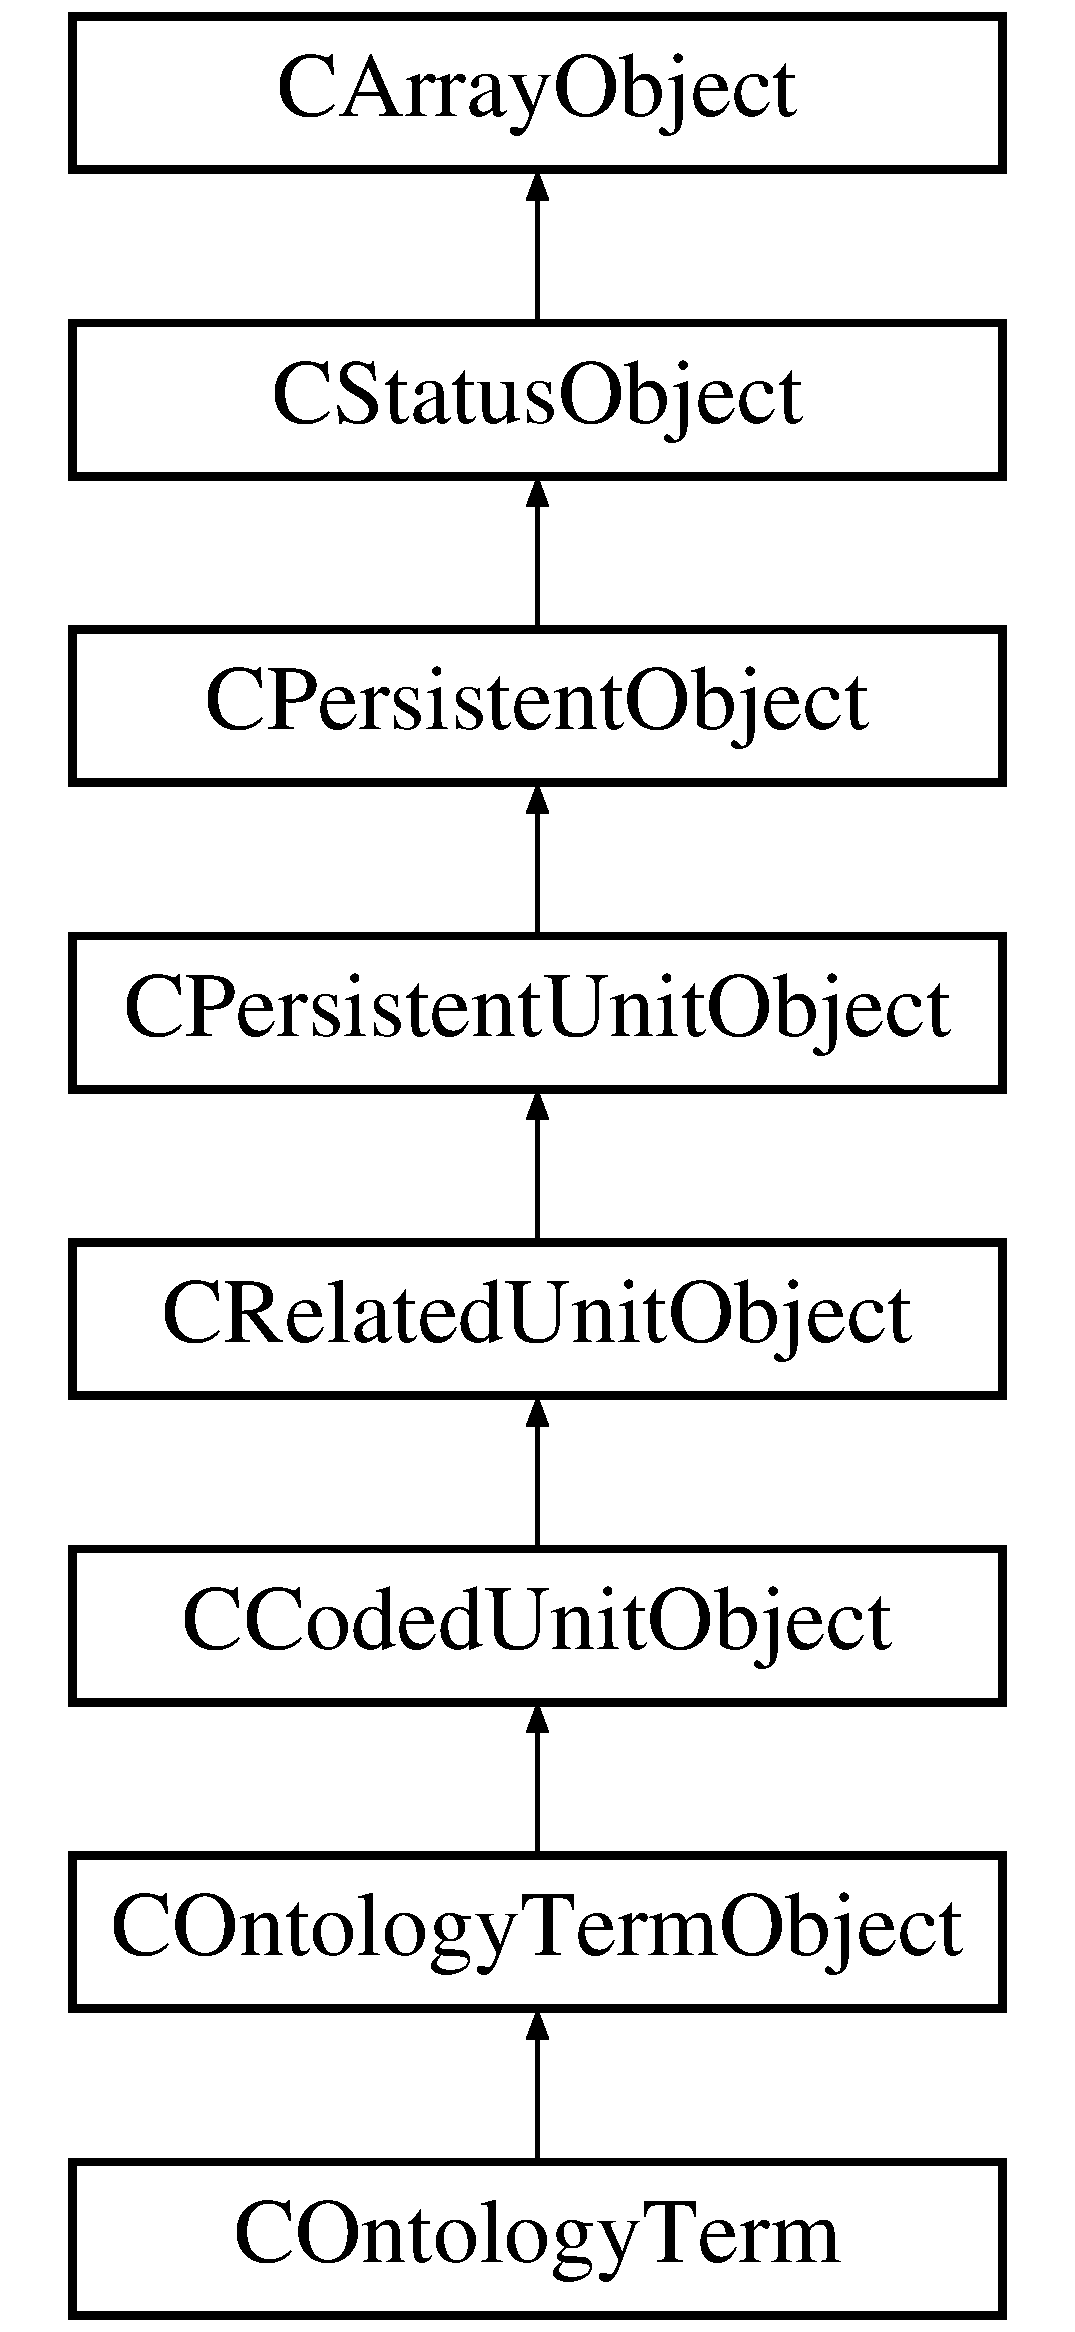
\includegraphics[height=9.000000cm]{class_c_ontology_term}
\end{center}
\end{figure}
\subsection*{Public Member Functions}
\begin{DoxyCompactItemize}
\item 
\hyperlink{class_c_ontology_term_a33679101b2a63044f0084918a8df123e}{\-\_\-\-\_\-construct} (\$the\-Container=N\-U\-L\-L, \$the\-Identifier=N\-U\-L\-L, \$the\-Modifiers=k\-F\-L\-A\-G\-\_\-\-D\-E\-F\-A\-U\-L\-T)
\item 
\hyperlink{class_c_ontology_term_a86fd6d9e2c98a68c1600975f18793239}{Node} (\$the\-Value=N\-U\-L\-L, \$the\-Operation=N\-U\-L\-L, \$get\-Old=F\-A\-L\-S\-E)
\item 
\hyperlink{class_c_ontology_term_aa275beb37c6697a8b9a6a6685f829afb}{Predicate} (\$the\-Value=N\-U\-L\-L, \$the\-Operation=N\-U\-L\-L, \$get\-Old=F\-A\-L\-S\-E)
\item 
\hyperlink{class_c_ontology_term_acbffa05d49c87a82d4ff71e93d3e732c}{Enumeration} (\$the\-Value=N\-U\-L\-L, \$the\-Operation=N\-U\-L\-L, \$get\-Old=F\-A\-L\-S\-E)
\item 
\hyperlink{class_c_ontology_term_afd46ef8241b696e99cf7b5e1334914b7}{Type} (\$the\-Value=N\-U\-L\-L, \$get\-Old=F\-A\-L\-S\-E)
\item 
\hyperlink{class_c_ontology_term_a6cf8cb14d45aae044d61ce8cab211d92}{Pattern} (\$the\-Value=N\-U\-L\-L, \$the\-Operation=N\-U\-L\-L, \$get\-Old=F\-A\-L\-S\-E)
\item 
\hyperlink{class_c_ontology_term_a0115abc39300d18a7d35014850d18a2e}{Cardinality} (\$the\-Value=N\-U\-L\-L, \$get\-Old=F\-A\-L\-S\-E)
\item 
\hyperlink{class_c_ontology_term_a81d71459e7696a821bdacaae7166483f}{Unit} (\$the\-Value=N\-U\-L\-L, \$get\-Old=F\-A\-L\-S\-E)
\item 
\hyperlink{class_c_ontology_term_a88a9743b98281665517ef3d5c16bed4c}{Examples} (\$the\-Value=N\-U\-L\-L, \$the\-Operation=N\-U\-L\-L, \$get\-Old=F\-A\-L\-S\-E)
\item 
\hyperlink{class_c_ontology_term_aba486e72f54e61651a75da75215aaa7c}{offset\-Set} (\$the\-Offset, \$the\-Value)
\item 
\hyperlink{class_c_ontology_term_a622c31b9466e49a1413d38fda9ef9bb1}{offset\-Unset} (\$the\-Offset)
\end{DoxyCompactItemize}
\subsection*{Protected Member Functions}
\begin{DoxyCompactItemize}
\item 
\hyperlink{class_c_ontology_term_a5d10f6baf1e484591d1d99b325e22d89}{\-\_\-\-Prepare\-Commit} (\&\$the\-Container, \&\$the\-Identifier, \&\$the\-Modifiers)
\item 
\hyperlink{class_c_ontology_term_a29fccef02b48fbf3fa63b4865f73ffe1}{\-\_\-\-Inited} ()
\end{DoxyCompactItemize}
\subsection*{Additional Inherited Members}


\subsection{Constructor \& Destructor Documentation}
\hypertarget{class_c_ontology_term_a33679101b2a63044f0084918a8df123e}{\index{C\-Ontology\-Term@{C\-Ontology\-Term}!\-\_\-\-\_\-construct@{\-\_\-\-\_\-construct}}
\index{\-\_\-\-\_\-construct@{\-\_\-\-\_\-construct}!COntologyTerm@{C\-Ontology\-Term}}
\subsubsection[{\-\_\-\-\_\-construct}]{\setlength{\rightskip}{0pt plus 5cm}C\-Ontology\-Term\-::\-\_\-\-\_\-construct (
\begin{DoxyParamCaption}
\item[{}]{\$the\-Container = {\ttfamily NULL}, }
\item[{}]{\$the\-Identifier = {\ttfamily NULL}, }
\item[{}]{\$the\-Modifiers = {\ttfamily kFLAG\-\_\-DEFAULT}}
\end{DoxyParamCaption}
)}}\label{class_c_ontology_term_a33679101b2a63044f0084918a8df123e}
Instantiate class.

We \hyperlink{class_c_coded_unit_object_a314fc62af62314f5ac5acca2ac809900}{overload} the constructor to initialise the \hyperlink{class_c_status_object_a8429102e4f52f7558649b64f4e673a69}{inited} \hyperlink{}{flag} if the \hyperlink{class_c_coded_unit_object_a56af949800e65f9a283239d2e455259f}{code} and \hyperlink{class_c_term_a67e5776ea8799b3e68d2ed9ca6dcde58}{name} attributes are set.


\begin{DoxyParams}[1]{Parameters}
mixed & {\em \$the\-Container} & Persistent container. \\
\hline
mixed & {\em \$the\-Identifier} & Object identifier. \\
\hline
bitfield & {\em \$the\-Modifiers} & Create modifiers.\\
\hline
\end{DoxyParams}
public

\-\_\-\-Is\-Inited

\begin{DoxySeeAlso}{See also}
k\-T\-A\-G\-\_\-\-C\-O\-D\-E k\-T\-A\-G\-\_\-\-N\-A\-M\-E 
\end{DoxySeeAlso}


Reimplemented from \hyperlink{class_c_ontology_term_object_af1fb502088538ad7372719c20f73bc5c}{C\-Ontology\-Term\-Object}.



\subsection{Member Function Documentation}
\hypertarget{class_c_ontology_term_a29fccef02b48fbf3fa63b4865f73ffe1}{\index{C\-Ontology\-Term@{C\-Ontology\-Term}!\-\_\-\-Inited@{\-\_\-\-Inited}}
\index{\-\_\-\-Inited@{\-\_\-\-Inited}!COntologyTerm@{C\-Ontology\-Term}}
\subsubsection[{\-\_\-\-Inited}]{\setlength{\rightskip}{0pt plus 5cm}C\-Ontology\-Term\-::\-\_\-\-Inited (
\begin{DoxyParamCaption}
{}
\end{DoxyParamCaption}
)\hspace{0.3cm}{\ttfamily [protected]}}}\label{class_c_ontology_term_a29fccef02b48fbf3fa63b4865f73ffe1}
Return \hyperlink{class_c_status_object_a8429102e4f52f7558649b64f4e673a69}{initialised} status.

This method will check the contents of the object and return the correct \hyperlink{class_c_status_object_a8429102e4f52f7558649b64f4e673a69}{initialised} status according to the contents of the \hyperlink{class_c_coded_unit_object_aafe9f12551f9f183c21a9865f0e9c670}{kind} \hyperlink{}{property}\-:


\begin{DoxyItemize}
\item {\itshape Default}\-: By default the object must have its \hyperlink{}{code} set, this is \hyperlink{class_c_ontology_term_object}{inherited}. 
\item {\itshape \hyperlink{}{k\-T\-Y\-P\-E\-\_\-\-N\-A\-M\-E\-S\-P\-A\-C\-E}}\-: It uses the default requirements. 
\item {\itshape \hyperlink{}{k\-T\-Y\-P\-E\-\_\-\-R\-O\-O\-T}}\-: It requires the \hyperlink{}{name}. 
\item {\itshape \hyperlink{}{k\-T\-Y\-P\-E\-\_\-\-P\-R\-E\-D\-I\-C\-A\-T\-E}}\-: It requires the \hyperlink{}{name}. 
\item {\itshape \hyperlink{}{k\-T\-Y\-P\-E\-\_\-\-A\-T\-T\-R\-I\-B\-U\-T\-E}}\-: It requires the \hyperlink{}{name} and \hyperlink{}{cardinality}. 
\item {\itshape \hyperlink{}{k\-T\-Y\-P\-E\-\_\-\-M\-E\-A\-S\-U\-R\-E}}\-: It requires the \hyperlink{}{name} and \hyperlink{}{type}. 
\item {\itshape \hyperlink{}{k\-T\-Y\-P\-E\-\_\-\-E\-N\-U\-M\-E\-R\-A\-T\-I\-O\-N}}\-: It requires the \hyperlink{}{name} and \hyperlink{}{enumeration}. 
\end{DoxyItemize}

protected \begin{DoxyReturn}{Returns}
boolean 
\end{DoxyReturn}
\hypertarget{class_c_ontology_term_a5d10f6baf1e484591d1d99b325e22d89}{\index{C\-Ontology\-Term@{C\-Ontology\-Term}!\-\_\-\-Prepare\-Commit@{\-\_\-\-Prepare\-Commit}}
\index{\-\_\-\-Prepare\-Commit@{\-\_\-\-Prepare\-Commit}!COntologyTerm@{C\-Ontology\-Term}}
\subsubsection[{\-\_\-\-Prepare\-Commit}]{\setlength{\rightskip}{0pt plus 5cm}C\-Ontology\-Term\-::\-\_\-\-Prepare\-Commit (
\begin{DoxyParamCaption}
\item[{\&}]{\$the\-Container, }
\item[{\&}]{\$the\-Identifier, }
\item[{\&}]{\$the\-Modifiers}
\end{DoxyParamCaption}
)\hspace{0.3cm}{\ttfamily [protected]}}}\label{class_c_ontology_term_a5d10f6baf1e484591d1d99b325e22d89}
Normalise before a store.

We overload this method to set default \hyperlink{class_c_coded_unit_object_aafe9f12551f9f183c21a9865f0e9c670}{kinds} according to which data properties the object has\-:


\begin{DoxyItemize}
\item {\itshape \hyperlink{class_c_ontology_term_a0115abc39300d18a7d35014850d18a2e}{Cardinality}}\-: We set the \hyperlink{class_c_coded_unit_object_aafe9f12551f9f183c21a9865f0e9c670}{kind} to \hyperlink{}{attribute}. 
\item {\itshape Data \hyperlink{class_c_ontology_term_afd46ef8241b696e99cf7b5e1334914b7}{Type}}\-: We set the \hyperlink{class_c_coded_unit_object_aafe9f12551f9f183c21a9865f0e9c670}{kind} to \hyperlink{}{measure}. 
\item {\itshape \hyperlink{class_c_ontology_term_acbffa05d49c87a82d4ff71e93d3e732c}{Enumeration}}\-: We set the \hyperlink{class_c_coded_unit_object_aafe9f12551f9f183c21a9865f0e9c670}{kind} to \hyperlink{}{enumeration}. 
\end{DoxyItemize}

We also set by default the \hyperlink{}{enumeration} to the value of the \hyperlink{class_c_coded_unit_object_a56af949800e65f9a283239d2e455259f}{code}, if the term has the \hyperlink{}{enumeration} \hyperlink{class_c_coded_unit_object_aafe9f12551f9f183c21a9865f0e9c670}{kind} and the term \hyperlink{class_c_ontology_term_acbffa05d49c87a82d4ff71e93d3e732c}{enumerations} are empty.


\begin{DoxyParams}[1]{Parameters}
reference & {\em \&\$the\-Container} & Object container. \\
\hline
reference & {\em \&\$the\-Identifier} & Object identifier. \\
\hline
reference & {\em \&\$the\-Modifiers} & Commit modifiers.\\
\hline
\end{DoxyParams}
protected


\begin{DoxyExceptions}{Exceptions}
{\em \{@link} & \hyperlink{class_c_exception}{C\-Exception} \hyperlink{class_c_exception}{C\-Exception}\}\\
\hline
\end{DoxyExceptions}
\hyperlink{class_c_coded_unit_object_aafe9f12551f9f183c21a9865f0e9c670}{Kind()}

\begin{DoxySeeAlso}{See also}
k\-T\-Y\-P\-E\-\_\-\-E\-N\-U\-M\-E\-R\-A\-T\-I\-O\-N 
\end{DoxySeeAlso}


Reimplemented from \hyperlink{class_c_ontology_term_object_aca3572974abb180f507fc63264a9ba15}{C\-Ontology\-Term\-Object}.

\hypertarget{class_c_ontology_term_a0115abc39300d18a7d35014850d18a2e}{\index{C\-Ontology\-Term@{C\-Ontology\-Term}!Cardinality@{Cardinality}}
\index{Cardinality@{Cardinality}!COntologyTerm@{C\-Ontology\-Term}}
\subsubsection[{Cardinality}]{\setlength{\rightskip}{0pt plus 5cm}C\-Ontology\-Term\-::\-Cardinality (
\begin{DoxyParamCaption}
\item[{}]{\$the\-Value = {\ttfamily NULL}, }
\item[{}]{\$get\-Old = {\ttfamily FALSE}}
\end{DoxyParamCaption}
)}}\label{class_c_ontology_term_a0115abc39300d18a7d35014850d18a2e}
Manage data cardinality.

This method can be used to manage the measure data \hyperlink{}{type}, it uses the standard accessor \hyperlink{class_c_attribute_a9d231a47718719fcd6c33f3d0ac91675}{method} to manage the \hyperlink{}{offset}\-:


\begin{DoxyItemize}
\item {\bfseries \$the\-Value}\-: The value or operation\-: 
\begin{DoxyItemize}
\item {\itshape N\-U\-L\-L}\-: Return the current value. 
\item {\itshape F\-A\-L\-S\-E}\-: Delete the value. 
\item {\itshape string}\-: String values represent the cardinality enumeration\-: 
\begin{DoxyItemize}
\item {\itshape \hyperlink{}{k\-C\-A\-R\-D\-\_\-0\-\_\-1}}\-: Zero or one, a scalar or none. 
\item {\itshape \hyperlink{}{k\-C\-A\-R\-D\-\_\-1}}\-: Exactly one, a required scalar. 
\item {\itshape \hyperlink{}{k\-C\-A\-R\-D\-\_\-\-A\-N\-Y}}\-: Any, this implies that we either have an array or no data. 
\end{DoxyItemize}
\item {\itshape integer}\-: An integer represents the exact cardinality, in that case we assume the data is an array of at most that number of elements. 
\end{DoxyItemize}
\item {\bfseries \$get\-Old}\-: Determines what the method will return\-: 
\begin{DoxyItemize}
\item {\itshape T\-R\-U\-E}\-: Return the value {\itshape before} it was eventually modified. 
\item {\itshape F\-A\-L\-S\-E}\-: Return the value {\itshape after} it was eventually modified. 
\end{DoxyItemize}
\end{DoxyItemize}


\begin{DoxyParams}[1]{Parameters}
N\-U\-L\-L | F\-A\-L\-S\-E | string & {\em \$the\-Value} & Data type tag. \\
\hline
boolean & {\em \$get\-Old} & T\-R\-U\-E get old value.\\
\hline
\end{DoxyParams}
public \begin{DoxyReturn}{Returns}
string 
\end{DoxyReturn}
\hypertarget{class_c_ontology_term_acbffa05d49c87a82d4ff71e93d3e732c}{\index{C\-Ontology\-Term@{C\-Ontology\-Term}!Enumeration@{Enumeration}}
\index{Enumeration@{Enumeration}!COntologyTerm@{C\-Ontology\-Term}}
\subsubsection[{Enumeration}]{\setlength{\rightskip}{0pt plus 5cm}C\-Ontology\-Term\-::\-Enumeration (
\begin{DoxyParamCaption}
\item[{}]{\$the\-Value = {\ttfamily NULL}, }
\item[{}]{\$the\-Operation = {\ttfamily NULL}, }
\item[{}]{\$get\-Old = {\ttfamily FALSE}}
\end{DoxyParamCaption}
)}}\label{class_c_ontology_term_acbffa05d49c87a82d4ff71e93d3e732c}
Manage enumerations.

This method can be used to handle the object's \hyperlink{}{enumerations}, it uses the standard accessor \hyperlink{class_c_attribute_a7d2e35b120eaa55529f78253f77dab48}{method} to manage the list of enumerations.

Each element of this list should indicate a code or acronym defining the current object

For a more thorough reference of how this method works, please consult the \hyperlink{class_c_attribute_a7d2e35b120eaa55529f78253f77dab48}{C\-Attribute\-::\-Manage\-Array\-Offset} method, in which the second parameter will be the constant \hyperlink{}{k\-T\-A\-G\-\_\-\-E\-N\-U\-M}.


\begin{DoxyParams}[1]{Parameters}
mixed & {\em \$the\-Value} & Value or index. \\
\hline
mixed & {\em \$the\-Operation} & Operation. \\
\hline
boolean & {\em \$get\-Old} & T\-R\-U\-E get old value.\\
\hline
\end{DoxyParams}
public \begin{DoxyReturn}{Returns}
mixed
\end{DoxyReturn}
\hyperlink{class_c_attribute_a7d2e35b120eaa55529f78253f77dab48}{C\-Attribute\-::\-Manage\-Array\-Offset()}

\begin{DoxySeeAlso}{See also}
k\-T\-A\-G\-\_\-\-E\-N\-U\-M 
\end{DoxySeeAlso}
\hypertarget{class_c_ontology_term_a88a9743b98281665517ef3d5c16bed4c}{\index{C\-Ontology\-Term@{C\-Ontology\-Term}!Examples@{Examples}}
\index{Examples@{Examples}!COntologyTerm@{C\-Ontology\-Term}}
\subsubsection[{Examples}]{\setlength{\rightskip}{0pt plus 5cm}C\-Ontology\-Term\-::\-Examples (
\begin{DoxyParamCaption}
\item[{}]{\$the\-Value = {\ttfamily NULL}, }
\item[{}]{\$the\-Operation = {\ttfamily NULL}, }
\item[{}]{\$get\-Old = {\ttfamily FALSE}}
\end{DoxyParamCaption}
)}}\label{class_c_ontology_term_a88a9743b98281665517ef3d5c16bed4c}
Manage data examples.

This method can be used to handle data \hyperlink{}{examples}, it is a list of strings handles by the standard accessor \hyperlink{class_c_attribute_a7d2e35b120eaa55529f78253f77dab48}{method} in the examples \hyperlink{}{offset}.

The provided value should be an example of how the current term could be represented, an extensive set of examples should be included in order to provide enough information to handle correctly any kind of output referenced data elements could represent.

For a more in-\/depth reference of this method, please consult the \hyperlink{class_c_attribute_a7d2e35b120eaa55529f78253f77dab48}{C\-Attribute\-::\-Manage\-Array\-Offset} method, in which the second parameter will be the constant \hyperlink{}{k\-T\-A\-G\-\_\-\-V\-A\-L\-I\-D}.


\begin{DoxyParams}[1]{Parameters}
mixed & {\em \$the\-Value} & Value or index. \\
\hline
mixed & {\em \$the\-Operation} & Operation. \\
\hline
boolean & {\em \$get\-Old} & T\-R\-U\-E get old value.\\
\hline
\end{DoxyParams}
public \begin{DoxyReturn}{Returns}
string
\end{DoxyReturn}
\hyperlink{class_c_attribute_a7d2e35b120eaa55529f78253f77dab48}{C\-Attribute\-::\-Manage\-Array\-Offset()}

\begin{DoxySeeAlso}{See also}
k\-T\-A\-G\-\_\-\-E\-X\-A\-M\-P\-L\-E\-S 
\end{DoxySeeAlso}
\hypertarget{class_c_ontology_term_a86fd6d9e2c98a68c1600975f18793239}{\index{C\-Ontology\-Term@{C\-Ontology\-Term}!Node@{Node}}
\index{Node@{Node}!COntologyTerm@{C\-Ontology\-Term}}
\subsubsection[{Node}]{\setlength{\rightskip}{0pt plus 5cm}C\-Ontology\-Term\-::\-Node (
\begin{DoxyParamCaption}
\item[{}]{\$the\-Value = {\ttfamily NULL}, }
\item[{}]{\$the\-Operation = {\ttfamily NULL}, }
\item[{}]{\$get\-Old = {\ttfamily FALSE}}
\end{DoxyParamCaption}
)}}\label{class_c_ontology_term_a86fd6d9e2c98a68c1600975f18793239}
Manage node references.

This method can be used to handle the object's \hyperlink{}{node} references, it uses the standard accessor \hyperlink{class_c_attribute_a7d2e35b120eaa55529f78253f77dab48}{method} to manage the list of nodes that point to this term.

Each element of this list represents the I\-D of a node in the ontology\-: each time a node references this term, its identifier will be aded to this offset.

For a more thorough reference of how this method works, please consult the \hyperlink{class_c_attribute_a7d2e35b120eaa55529f78253f77dab48}{C\-Attribute\-::\-Manage\-Array\-Offset} method, in which the second parameter will be the constant \hyperlink{}{k\-T\-A\-G\-\_\-\-K\-I\-N\-D}.

Note that you should only use this method for retrieving information, since \hyperlink{class_c_ontology_node}{nodes} store automatically this information when \hyperlink{class_c_persistent_object_a88b1f2b11d3d60e0b3d33d8b0649b68a}{saved}.


\begin{DoxyParams}[1]{Parameters}
mixed & {\em \$the\-Value} & Value or index. \\
\hline
mixed & {\em \$the\-Operation} & Operation. \\
\hline
boolean & {\em \$get\-Old} & T\-R\-U\-E get old value.\\
\hline
\end{DoxyParams}
public \begin{DoxyReturn}{Returns}
mixed
\end{DoxyReturn}
\hyperlink{class_c_attribute_a7d2e35b120eaa55529f78253f77dab48}{C\-Attribute\-::\-Manage\-Array\-Offset()}

\begin{DoxySeeAlso}{See also}
k\-T\-A\-G\-\_\-\-N\-O\-D\-E 
\end{DoxySeeAlso}
\hypertarget{class_c_ontology_term_aba486e72f54e61651a75da75215aaa7c}{\index{C\-Ontology\-Term@{C\-Ontology\-Term}!offset\-Set@{offset\-Set}}
\index{offset\-Set@{offset\-Set}!COntologyTerm@{C\-Ontology\-Term}}
\subsubsection[{offset\-Set}]{\setlength{\rightskip}{0pt plus 5cm}C\-Ontology\-Term\-::offset\-Set (
\begin{DoxyParamCaption}
\item[{}]{\$the\-Offset, }
\item[{}]{\$the\-Value}
\end{DoxyParamCaption}
)}}\label{class_c_ontology_term_aba486e72f54e61651a75da75215aaa7c}
Set a value for a given offset.

We overload this method to manage the \hyperlink{class_c_status_object_a8429102e4f52f7558649b64f4e673a69}{inited} \hyperlink{}{status}\-: this is set if the \hyperlink{class_c_coded_unit_object_a56af949800e65f9a283239d2e455259f}{code} and \hyperlink{class_c_term_a67e5776ea8799b3e68d2ed9ca6dcde58}{name} attributes are set.


\begin{DoxyParams}[1]{Parameters}
string & {\em \$the\-Offset} & Offset. \\
\hline
string | N\-U\-L\-L & {\em \$the\-Value} & Value to set at offset.\\
\hline
\end{DoxyParams}
public 

Reimplemented from \hyperlink{class_c_coded_unit_object_a49bb8f2956cb0551ba827b222778f295}{C\-Coded\-Unit\-Object}.

\hypertarget{class_c_ontology_term_a622c31b9466e49a1413d38fda9ef9bb1}{\index{C\-Ontology\-Term@{C\-Ontology\-Term}!offset\-Unset@{offset\-Unset}}
\index{offset\-Unset@{offset\-Unset}!COntologyTerm@{C\-Ontology\-Term}}
\subsubsection[{offset\-Unset}]{\setlength{\rightskip}{0pt plus 5cm}C\-Ontology\-Term\-::offset\-Unset (
\begin{DoxyParamCaption}
\item[{}]{\$the\-Offset}
\end{DoxyParamCaption}
)}}\label{class_c_ontology_term_a622c31b9466e49a1413d38fda9ef9bb1}
Reset a value for a given offset.

We overload this method to manage the \hyperlink{class_c_status_object_a8429102e4f52f7558649b64f4e673a69}{inited} \hyperlink{}{status}\-: this is set if the \hyperlink{class_c_coded_unit_object_a56af949800e65f9a283239d2e455259f}{code} and \hyperlink{class_c_term_a67e5776ea8799b3e68d2ed9ca6dcde58}{name} attributes are set.


\begin{DoxyParams}[1]{Parameters}
string & {\em \$the\-Offset} & Offset.\\
\hline
\end{DoxyParams}
public 

Reimplemented from \hyperlink{class_c_coded_unit_object_a5072e0f72c19260df212a4cf93c9f1cb}{C\-Coded\-Unit\-Object}.

\hypertarget{class_c_ontology_term_a6cf8cb14d45aae044d61ce8cab211d92}{\index{C\-Ontology\-Term@{C\-Ontology\-Term}!Pattern@{Pattern}}
\index{Pattern@{Pattern}!COntologyTerm@{C\-Ontology\-Term}}
\subsubsection[{Pattern}]{\setlength{\rightskip}{0pt plus 5cm}C\-Ontology\-Term\-::\-Pattern (
\begin{DoxyParamCaption}
\item[{}]{\$the\-Value = {\ttfamily NULL}, }
\item[{}]{\$the\-Operation = {\ttfamily NULL}, }
\item[{}]{\$get\-Old = {\ttfamily FALSE}}
\end{DoxyParamCaption}
)}}\label{class_c_ontology_term_a6cf8cb14d45aae044d61ce8cab211d92}
Manage patterns.

This method can be used to handle the object's \hyperlink{}{patterns}, it uses the standard accessor \hyperlink{class_c_attribute_a7d2e35b120eaa55529f78253f77dab48}{method} to manage the list of patterns.

This term usually describes a \hyperlink{}{string} data element that is restricted by a series of string patterns, use the standard X\-M\-L format.

For a more thorough reference of how this method works, please consult the \hyperlink{class_c_attribute_a7d2e35b120eaa55529f78253f77dab48}{C\-Attribute\-::\-Manage\-Array\-Offset} method, in which the second parameter will be the constant \hyperlink{}{k\-T\-A\-G\-\_\-\-P\-A\-T\-T\-E\-R\-N}.


\begin{DoxyParams}[1]{Parameters}
mixed & {\em \$the\-Value} & Value or index. \\
\hline
mixed & {\em \$the\-Operation} & Operation. \\
\hline
boolean & {\em \$get\-Old} & T\-R\-U\-E get old value.\\
\hline
\end{DoxyParams}
public \begin{DoxyReturn}{Returns}
mixed
\end{DoxyReturn}
\hyperlink{class_c_attribute_a7d2e35b120eaa55529f78253f77dab48}{C\-Attribute\-::\-Manage\-Array\-Offset()}

\begin{DoxySeeAlso}{See also}
k\-T\-A\-G\-\_\-\-P\-A\-T\-T\-E\-R\-N 
\end{DoxySeeAlso}
\hypertarget{class_c_ontology_term_aa275beb37c6697a8b9a6a6685f829afb}{\index{C\-Ontology\-Term@{C\-Ontology\-Term}!Predicate@{Predicate}}
\index{Predicate@{Predicate}!COntologyTerm@{C\-Ontology\-Term}}
\subsubsection[{Predicate}]{\setlength{\rightskip}{0pt plus 5cm}C\-Ontology\-Term\-::\-Predicate (
\begin{DoxyParamCaption}
\item[{}]{\$the\-Value = {\ttfamily NULL}, }
\item[{}]{\$the\-Operation = {\ttfamily NULL}, }
\item[{}]{\$get\-Old = {\ttfamily FALSE}}
\end{DoxyParamCaption}
)}}\label{class_c_ontology_term_aa275beb37c6697a8b9a6a6685f829afb}
Manage predicate node references.

This method can be used to handle the object's predicate \hyperlink{}{node} references, it uses the standard accessor \hyperlink{class_c_attribute_a7d2e35b120eaa55529f78253f77dab48}{method} to manage the list of predicate nodes that point to this term.

Each element of this list represents the I\-D of an edge node in the ontology\-: each time an edge node references this term, its identifier will be aded to this offset.

For a more thorough reference of how this method works, please consult the \hyperlink{class_c_attribute_a7d2e35b120eaa55529f78253f77dab48}{C\-Attribute\-::\-Manage\-Array\-Offset} method, in which the second parameter will be the constant \hyperlink{}{k\-T\-A\-G\-\_\-\-K\-I\-N\-D}.

Note that you should only use this method for retrieving information, since \hyperlink{class_c_ontology_node}{nodes} store automatically this information when \hyperlink{class_c_persistent_object_a88b1f2b11d3d60e0b3d33d8b0649b68a}{saved}.


\begin{DoxyParams}[1]{Parameters}
mixed & {\em \$the\-Value} & Value or index. \\
\hline
mixed & {\em \$the\-Operation} & Operation. \\
\hline
boolean & {\em \$get\-Old} & T\-R\-U\-E get old value.\\
\hline
\end{DoxyParams}
public \begin{DoxyReturn}{Returns}
mixed
\end{DoxyReturn}
\hyperlink{class_c_attribute_a7d2e35b120eaa55529f78253f77dab48}{C\-Attribute\-::\-Manage\-Array\-Offset()}

\begin{DoxySeeAlso}{See also}
k\-T\-A\-G\-\_\-\-E\-D\-G\-E 
\end{DoxySeeAlso}
\hypertarget{class_c_ontology_term_afd46ef8241b696e99cf7b5e1334914b7}{\index{C\-Ontology\-Term@{C\-Ontology\-Term}!Type@{Type}}
\index{Type@{Type}!COntologyTerm@{C\-Ontology\-Term}}
\subsubsection[{Type}]{\setlength{\rightskip}{0pt plus 5cm}C\-Ontology\-Term\-::\-Type (
\begin{DoxyParamCaption}
\item[{}]{\$the\-Value = {\ttfamily NULL}, }
\item[{}]{\$get\-Old = {\ttfamily FALSE}}
\end{DoxyParamCaption}
)}}\label{class_c_ontology_term_afd46ef8241b696e99cf7b5e1334914b7}
Manage data type.

This method can be used to manage the measure data \hyperlink{}{type}, it uses the standard accessor \hyperlink{class_c_attribute_a9d231a47718719fcd6c33f3d0ac91675}{method} to manage the \hyperlink{}{offset}\-:


\begin{DoxyItemize}
\item {\bfseries \$the\-Value}\-: The value or operation\-: 
\begin{DoxyItemize}
\item {\itshape N\-U\-L\-L}\-: Return the current value. 
\item {\itshape F\-A\-L\-S\-E}\-: Delete the value. 
\item {\itshape other}\-: Set value. 
\end{DoxyItemize}
\item {\bfseries \$get\-Old}\-: Determines what the method will return\-: 
\begin{DoxyItemize}
\item {\itshape T\-R\-U\-E}\-: Return the value {\itshape before} it was eventually modified. 
\item {\itshape F\-A\-L\-S\-E}\-: Return the value {\itshape after} it was eventually modified. 
\end{DoxyItemize}
\end{DoxyItemize}


\begin{DoxyParams}[1]{Parameters}
N\-U\-L\-L | F\-A\-L\-S\-E | string & {\em \$the\-Value} & Data type tag. \\
\hline
boolean & {\em \$get\-Old} & T\-R\-U\-E get old value.\\
\hline
\end{DoxyParams}
public \begin{DoxyReturn}{Returns}
string 
\end{DoxyReturn}
\hypertarget{class_c_ontology_term_a81d71459e7696a821bdacaae7166483f}{\index{C\-Ontology\-Term@{C\-Ontology\-Term}!Unit@{Unit}}
\index{Unit@{Unit}!COntologyTerm@{C\-Ontology\-Term}}
\subsubsection[{Unit}]{\setlength{\rightskip}{0pt plus 5cm}C\-Ontology\-Term\-::\-Unit (
\begin{DoxyParamCaption}
\item[{}]{\$the\-Value = {\ttfamily NULL}, }
\item[{}]{\$get\-Old = {\ttfamily FALSE}}
\end{DoxyParamCaption}
)}}\label{class_c_ontology_term_a81d71459e7696a821bdacaae7166483f}
Manage data unit.

This method can be used to handle the measure \hyperlink{}{unit}, it uses the standard accessor \hyperlink{class_c_attribute_a9d231a47718719fcd6c33f3d0ac91675}{method} to manage the \hyperlink{}{offset}.

The value provided to this property should be the \hyperlink{class_c_persistent_unit_object_ad1ca0920cf0df3c24351402f9afbf34b}{identifier} of a term hat defines a unit.

For a more in-\/depth reference of this method, please consult the \hyperlink{class_c_attribute_a9d231a47718719fcd6c33f3d0ac91675}{C\-Attribute\-::\-Manage\-Offset} method, in which the second parameter will be the constant \hyperlink{}{k\-T\-A\-G\-\_\-\-V\-A\-L\-I\-D}.

In this class we feed the value to the\hyperlink{class_c_ontology_term_object_a294971c8d6e1181b0b9ec98ab998d6a0}{\-\_\-\-Check\-Reference} method that will take care of handling object references.


\begin{DoxyParams}[1]{Parameters}
mixed & {\em \$the\-Value} & Value. \\
\hline
boolean & {\em \$get\-Old} & T\-R\-U\-E get old value.\\
\hline
\end{DoxyParams}
public \begin{DoxyReturn}{Returns}
string
\end{DoxyReturn}
\hyperlink{class_c_attribute_a9d231a47718719fcd6c33f3d0ac91675}{C\-Attribute\-::\-Manage\-Offset()}

\begin{DoxySeeAlso}{See also}
k\-T\-A\-G\-\_\-\-U\-N\-I\-T 
\end{DoxySeeAlso}


The documentation for this class was generated from the following file\-:\begin{DoxyCompactItemize}
\item 
/\-Library/\-Web\-Server/\-Library/wrapper/classes/C\-Ontology\-Term.\-php\end{DoxyCompactItemize}

\hypertarget{class_c_ontology_term_object}{\section{C\-Ontology\-Term\-Object Class Reference}
\label{class_c_ontology_term_object}\index{C\-Ontology\-Term\-Object@{C\-Ontology\-Term\-Object}}
}
Inheritance diagram for C\-Ontology\-Term\-Object\-:\begin{figure}[H]
\begin{center}
\leavevmode
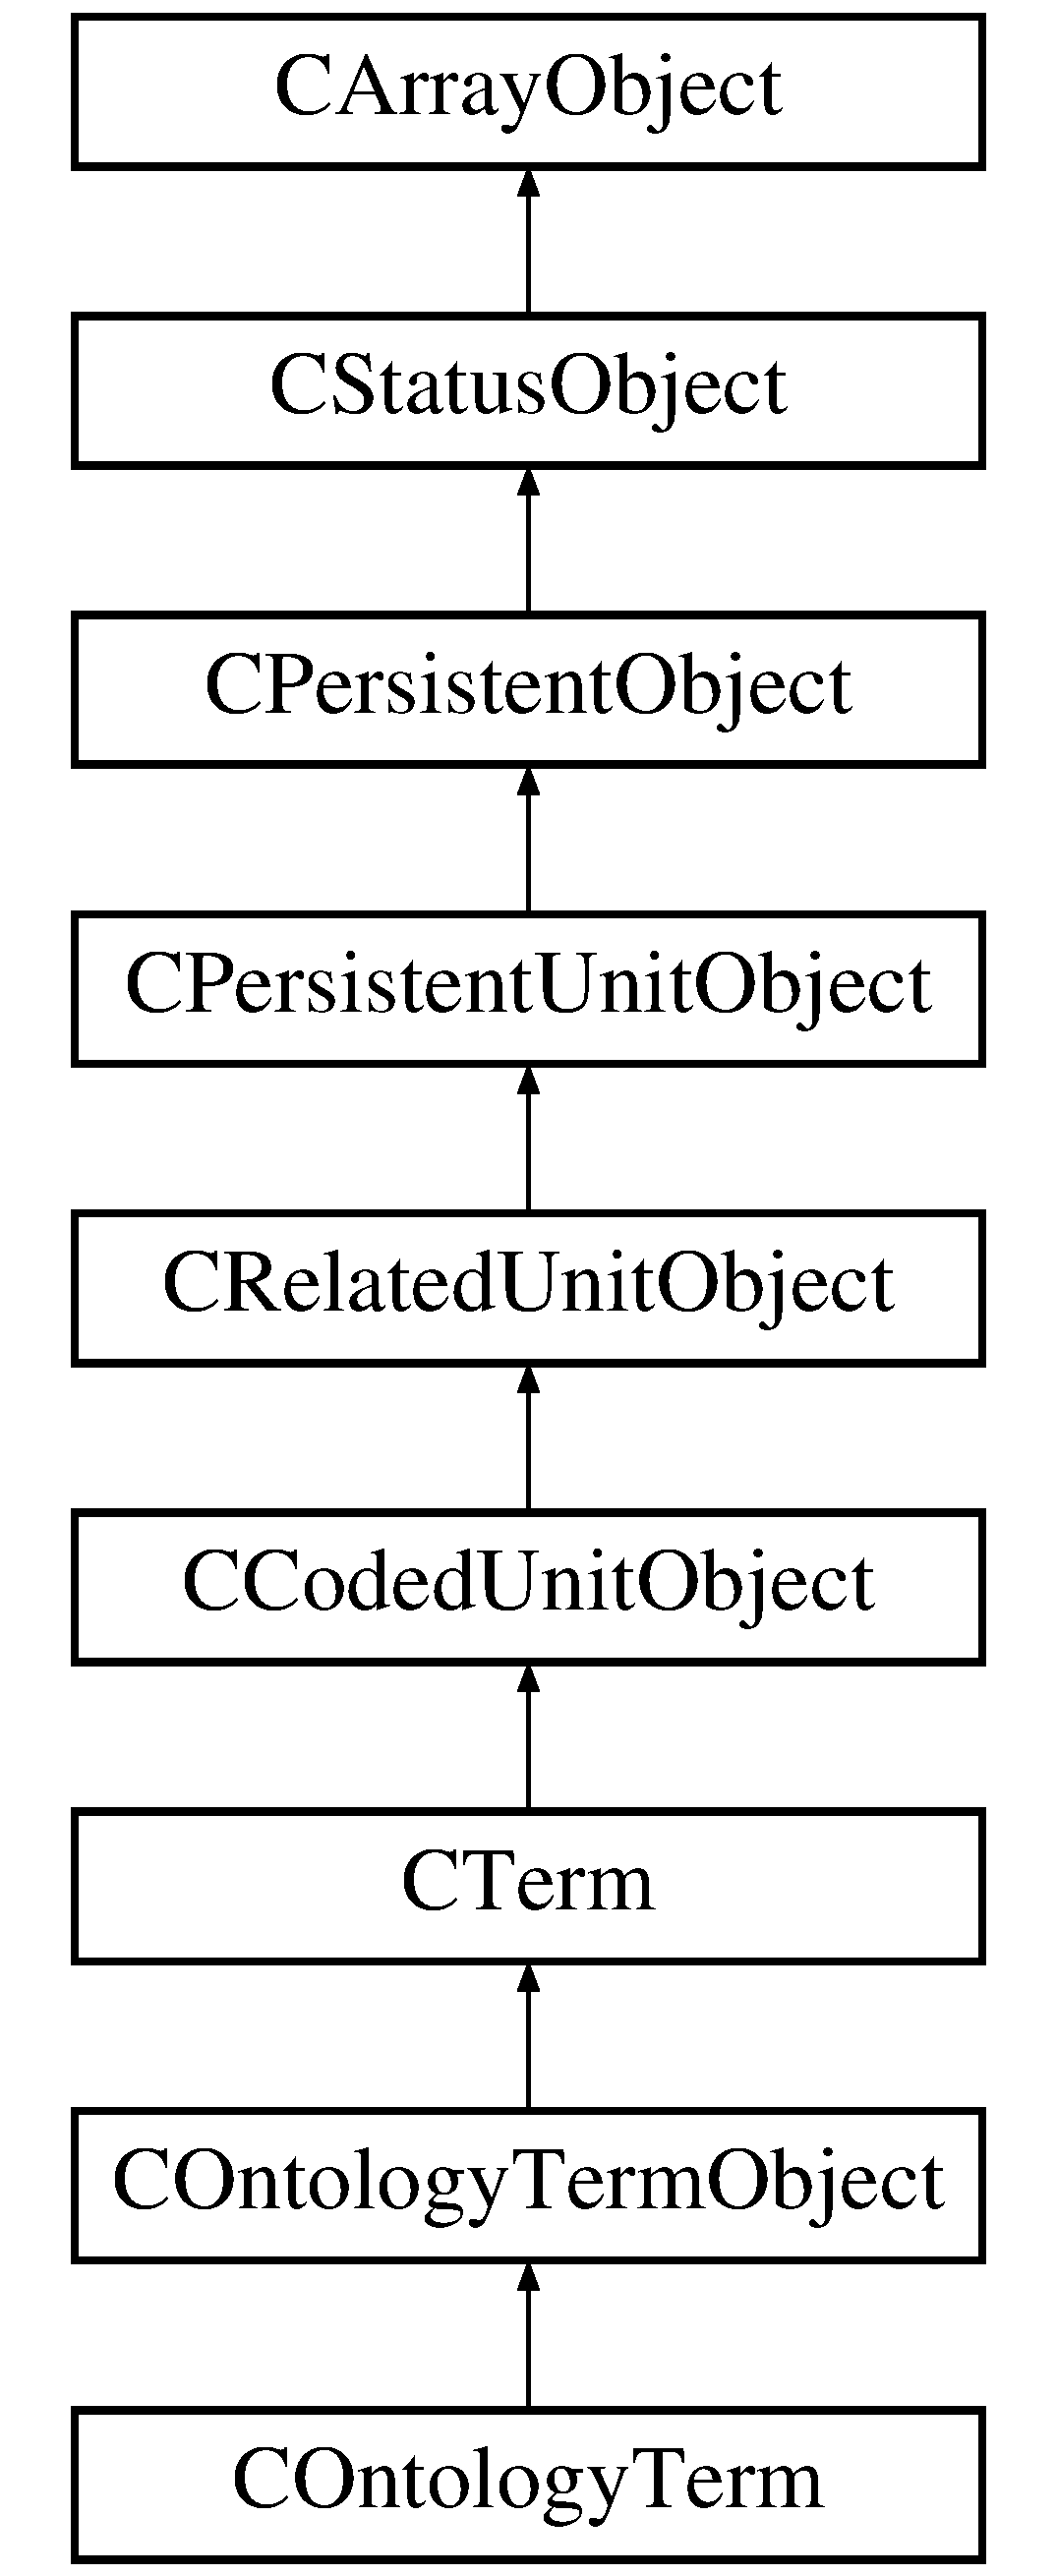
\includegraphics[height=9.000000cm]{class_c_ontology_term_object}
\end{center}
\end{figure}
\subsection*{Public Member Functions}
\begin{DoxyCompactItemize}
\item 
\hyperlink{class_c_ontology_term_object_af1fb502088538ad7372719c20f73bc5c}{\-\_\-\-\_\-construct} (\$the\-Container=N\-U\-L\-L, \$the\-Identifier=N\-U\-L\-L, \$the\-Modifiers=k\-F\-L\-A\-G\-\_\-\-D\-E\-F\-A\-U\-L\-T)
\item 
\hyperlink{class_c_ontology_term_object_a109414a9abe98e3997be238addfda6cf}{N\-S} (\$the\-Value=N\-U\-L\-L, \$get\-Old=F\-A\-L\-S\-E)
\item 
\hyperlink{class_c_ontology_term_object_ab1a4d21bb56a8a6cf3f77f595d776267}{G\-I\-D} ()
\item 
\hyperlink{class_c_ontology_term_object_a96f637a86e1823dc61b2135a00ddfe26}{Synonym} (\$the\-Value, \$the\-Type, \$the\-Operation=N\-U\-L\-L, \$get\-Old=F\-A\-L\-S\-E)
\item 
\hyperlink{class_c_ontology_term_object_a32bb224840f965d3c2680895b52847c4}{Xref} (\$the\-Value, \$the\-Type, \$the\-Operation=N\-U\-L\-L, \$get\-Old=F\-A\-L\-S\-E)
\item 
\hyperlink{class_c_ontology_term_object_ab023a6d801c93d939683da4fe823e0fb}{Relate} (\$the\-Object, \$the\-Predicate=N\-U\-L\-L, \$the\-Operation=N\-U\-L\-L, \$get\-Old=F\-A\-L\-S\-E)
\item 
\hyperlink{class_c_ontology_term_object_a41c7f8fbe4e561b744277fc62ba18912}{Valid} (\$the\-Value=N\-U\-L\-L, \$get\-Old=F\-A\-L\-S\-E)
\end{DoxyCompactItemize}
\subsection*{Static Public Member Functions}
\begin{DoxyCompactItemize}
\item 
static \hyperlink{class_c_ontology_term_object_a97ba6103f14e03000996ea6314de6444}{Valid\-Object} (\$the\-Container, \$the\-Identifier, \$the\-Modifiers=k\-F\-L\-A\-G\-\_\-\-D\-E\-F\-A\-U\-L\-T)
\end{DoxyCompactItemize}
\subsection*{Protected Member Functions}
\begin{DoxyCompactItemize}
\item 
\hyperlink{class_c_ontology_term_object_a7e785a79bf4c20b094450e688e3e73cf}{\-\_\-\-Prepare\-Create} (\&\$the\-Container, \&\$the\-Identifier, \&\$the\-Modifiers)
\item 
\hyperlink{class_c_ontology_term_object_aca3572974abb180f507fc63264a9ba15}{\-\_\-\-Prepare\-Commit} (\&\$the\-Container, \&\$the\-Identifier, \&\$the\-Modifiers)
\item 
\hyperlink{class_c_ontology_term_object_a294971c8d6e1181b0b9ec98ab998d6a0}{\-\_\-\-Check\-Reference} (\$the\-Reference)
\end{DoxyCompactItemize}


\subsection{Constructor \& Destructor Documentation}
\hypertarget{class_c_ontology_term_object_af1fb502088538ad7372719c20f73bc5c}{\index{C\-Ontology\-Term\-Object@{C\-Ontology\-Term\-Object}!\-\_\-\-\_\-construct@{\-\_\-\-\_\-construct}}
\index{\-\_\-\-\_\-construct@{\-\_\-\-\_\-construct}!COntologyTermObject@{C\-Ontology\-Term\-Object}}
\subsubsection[{\-\_\-\-\_\-construct}]{\setlength{\rightskip}{0pt plus 5cm}C\-Ontology\-Term\-Object\-::\-\_\-\-\_\-construct (
\begin{DoxyParamCaption}
\item[{}]{\$the\-Container = {\ttfamily NULL}, }
\item[{}]{\$the\-Identifier = {\ttfamily NULL}, }
\item[{}]{\$the\-Modifiers = {\ttfamily kFLAG\-\_\-DEFAULT}}
\end{DoxyParamCaption}
)}}\label{class_c_ontology_term_object_af1fb502088538ad7372719c20f73bc5c}
Instantiate class.

We \hyperlink{class_c_coded_unit_object_a314fc62af62314f5ac5acca2ac809900}{overload} the constructor to \hyperlink{class_c_ontology_term_object_a294971c8d6e1181b0b9ec98ab998d6a0}{normalise} the provided identifier.


\begin{DoxyParams}[1]{Parameters}
mixed & {\em \$the\-Container} & Persistent container. \\
\hline
mixed & {\em \$the\-Identifier} & Object identifier. \\
\hline
bitfield & {\em \$the\-Modifiers} & Create modifiers.\\
\hline
\end{DoxyParams}
public

\-\_\-\-Is\-Inited

\begin{DoxySeeAlso}{See also}
k\-T\-A\-G\-\_\-\-C\-O\-D\-E k\-T\-A\-G\-\_\-\-N\-A\-M\-E 
\end{DoxySeeAlso}


Reimplemented from \hyperlink{class_c_coded_unit_object_a314fc62af62314f5ac5acca2ac809900}{C\-Coded\-Unit\-Object}.



Reimplemented in \hyperlink{class_c_ontology_term_a33679101b2a63044f0084918a8df123e}{C\-Ontology\-Term}.



\subsection{Member Function Documentation}
\hypertarget{class_c_ontology_term_object_a294971c8d6e1181b0b9ec98ab998d6a0}{\index{C\-Ontology\-Term\-Object@{C\-Ontology\-Term\-Object}!\-\_\-\-Check\-Reference@{\-\_\-\-Check\-Reference}}
\index{\-\_\-\-Check\-Reference@{\-\_\-\-Check\-Reference}!COntologyTermObject@{C\-Ontology\-Term\-Object}}
\subsubsection[{\-\_\-\-Check\-Reference}]{\setlength{\rightskip}{0pt plus 5cm}C\-Ontology\-Term\-Object\-::\-\_\-\-Check\-Reference (
\begin{DoxyParamCaption}
\item[{}]{\$the\-Reference}
\end{DoxyParamCaption}
)\hspace{0.3cm}{\ttfamily [protected]}}}\label{class_c_ontology_term_object_a294971c8d6e1181b0b9ec98ab998d6a0}
Normalise reference parameter.

This method can be used to normalise a parameter that is supposed to be a reference to another term, that is, a binary string hash of the term's \hyperlink{class_c_term_a7524effdc0db8f5ca045f306e3b6b50e}{identifier} converted to a \hyperlink{class_c_data_type_binary}{binary} standard type.

The method will perform the following conversions\-:


\begin{DoxyItemize}
\item {\itshape \hyperlink{class_c_data_type_binary}{C\-Data\-Type\-Binary}}\-: This is the default data type for the identifier. 
\item {\itshape \hyperlink{}{Mongo\-Bin\-Data}}\-: This type will be converted to the standard \hyperlink{class_c_data_type_binary}{C\-Data\-Type\-Binary} type. 
\item {\itshape \hyperlink{class_c_ontology_term_object}{C\-Ontology\-Term\-Object}}\-: Objects of the same class will have their \hyperlink{class_c_persistent_unit_object_ad1ca0920cf0df3c24351402f9afbf34b}{identifier} extracted. 
\item {\itshape N\-U\-L\-L}\-: N\-U\-L\-L data will simply be passed. 
\item {\itshape other}\-: Any other data type is assumed to be the term's \hyperlink{class_c_term_a7524effdc0db8f5ca045f306e3b6b50e}{identifier}, so it will be hashed into a binary string and converted to the standard \hyperlink{class_c_data_type_binary}{C\-Data\-Type\-Binary} type. 
\item {\itshape array}\-: Arrays cannot be converted to string, so the method will raise an exception. 
\end{DoxyItemize}


\begin{DoxyParams}[1]{Parameters}
mixed & {\em \$the\-Reference} & Object reference.\\
\hline
\end{DoxyParams}
protected \begin{DoxyReturn}{Returns}
\hyperlink{class_c_data_type_binary}{C\-Data\-Type\-Binary}
\end{DoxyReturn}
\hyperlink{class_c_persistent_object_aa8dc7db66e2af3d28c2035161a2aabf9}{\-\_\-\-Is\-Encoded()}

\begin{DoxySeeAlso}{See also}
k\-F\-L\-A\-G\-\_\-\-S\-T\-A\-T\-E\-\_\-\-E\-N\-C\-O\-D\-E\-D 
\end{DoxySeeAlso}
\hypertarget{class_c_ontology_term_object_aca3572974abb180f507fc63264a9ba15}{\index{C\-Ontology\-Term\-Object@{C\-Ontology\-Term\-Object}!\-\_\-\-Prepare\-Commit@{\-\_\-\-Prepare\-Commit}}
\index{\-\_\-\-Prepare\-Commit@{\-\_\-\-Prepare\-Commit}!COntologyTermObject@{C\-Ontology\-Term\-Object}}
\subsubsection[{\-\_\-\-Prepare\-Commit}]{\setlength{\rightskip}{0pt plus 5cm}C\-Ontology\-Term\-Object\-::\-\_\-\-Prepare\-Commit (
\begin{DoxyParamCaption}
\item[{\&}]{\$the\-Container, }
\item[{\&}]{\$the\-Identifier, }
\item[{\&}]{\$the\-Modifiers}
\end{DoxyParamCaption}
)\hspace{0.3cm}{\ttfamily [protected]}}}\label{class_c_ontology_term_object_aca3572974abb180f507fc63264a9ba15}
Normalise before a store.

We overload this method to enforce the \hyperlink{}{encoded} modifier.


\begin{DoxyParams}[1]{Parameters}
reference & {\em \&\$the\-Container} & Object container. \\
\hline
reference & {\em \&\$the\-Identifier} & Object identifier. \\
\hline
reference & {\em \&\$the\-Modifiers} & Commit modifiers.\\
\hline
\end{DoxyParams}
protected


\begin{DoxyExceptions}{Exceptions}
{\em \{@link} & \hyperlink{class_c_exception}{C\-Exception} \hyperlink{class_c_exception}{C\-Exception}\}\\
\hline
\end{DoxyExceptions}
\hyperlink{class_c_status_object_a8429102e4f52f7558649b64f4e673a69}{\-\_\-\-Is\-Inited()}

\begin{DoxySeeAlso}{See also}
k\-F\-L\-A\-G\-\_\-\-S\-T\-A\-T\-E\-\_\-\-E\-N\-C\-O\-D\-E\-D 
\end{DoxySeeAlso}


Reimplemented from \hyperlink{class_c_related_unit_object_a577c73999830641e07440126a3252286}{C\-Related\-Unit\-Object}.



Reimplemented in \hyperlink{class_c_ontology_term_a5d10f6baf1e484591d1d99b325e22d89}{C\-Ontology\-Term}.

\hypertarget{class_c_ontology_term_object_a7e785a79bf4c20b094450e688e3e73cf}{\index{C\-Ontology\-Term\-Object@{C\-Ontology\-Term\-Object}!\-\_\-\-Prepare\-Create@{\-\_\-\-Prepare\-Create}}
\index{\-\_\-\-Prepare\-Create@{\-\_\-\-Prepare\-Create}!COntologyTermObject@{C\-Ontology\-Term\-Object}}
\subsubsection[{\-\_\-\-Prepare\-Create}]{\setlength{\rightskip}{0pt plus 5cm}C\-Ontology\-Term\-Object\-::\-\_\-\-Prepare\-Create (
\begin{DoxyParamCaption}
\item[{\&}]{\$the\-Container, }
\item[{\&}]{\$the\-Identifier, }
\item[{\&}]{\$the\-Modifiers}
\end{DoxyParamCaption}
)\hspace{0.3cm}{\ttfamily [protected]}}}\label{class_c_ontology_term_object_a7e785a79bf4c20b094450e688e3e73cf}
Normalise parameters of a create.

We overload this method to enforce the \hyperlink{}{encoded} modifier.


\begin{DoxyParams}[1]{Parameters}
reference & {\em \&\$the\-Container} & Object container. \\
\hline
reference & {\em \&\$the\-Identifier} & Object identifier. \\
\hline
reference & {\em \&\$the\-Modifiers} & Create modifiers.\\
\hline
\end{DoxyParams}
protected

\hyperlink{class_c_persistent_object_aa8dc7db66e2af3d28c2035161a2aabf9}{\-\_\-\-Is\-Encoded()}

\begin{DoxySeeAlso}{See also}
k\-F\-L\-A\-G\-\_\-\-S\-T\-A\-T\-E\-\_\-\-E\-N\-C\-O\-D\-E\-D 
\end{DoxySeeAlso}


Reimplemented from \hyperlink{class_c_persistent_object_a2e5dd4f8a92c0ada964ade712c9579b0}{C\-Persistent\-Object}.

\hypertarget{class_c_ontology_term_object_ab1a4d21bb56a8a6cf3f77f595d776267}{\index{C\-Ontology\-Term\-Object@{C\-Ontology\-Term\-Object}!G\-I\-D@{G\-I\-D}}
\index{G\-I\-D@{G\-I\-D}!COntologyTermObject@{C\-Ontology\-Term\-Object}}
\subsubsection[{G\-I\-D}]{\setlength{\rightskip}{0pt plus 5cm}C\-Ontology\-Term\-Object\-::\-G\-I\-D (
\begin{DoxyParamCaption}
{}
\end{DoxyParamCaption}
)}}\label{class_c_ontology_term_object_ab1a4d21bb56a8a6cf3f77f595d776267}
Manage term global identifier.

The term global \hyperlink{}{identifier} represents the un-\/hashed version of the term local \hyperlink{}{identifier}.

This value is set automatically by methods, so this method is read-\/only.

public \begin{DoxyReturn}{Returns}
string
\end{DoxyReturn}
\begin{DoxySeeAlso}{See also}
k\-T\-A\-G\-\_\-\-G\-I\-D 
\end{DoxySeeAlso}
\hypertarget{class_c_ontology_term_object_a109414a9abe98e3997be238addfda6cf}{\index{C\-Ontology\-Term\-Object@{C\-Ontology\-Term\-Object}!N\-S@{N\-S}}
\index{N\-S@{N\-S}!COntologyTermObject@{C\-Ontology\-Term\-Object}}
\subsubsection[{N\-S}]{\setlength{\rightskip}{0pt plus 5cm}C\-Ontology\-Term\-Object\-::\-N\-S (
\begin{DoxyParamCaption}
\item[{}]{\$the\-Value = {\ttfamily NULL}, }
\item[{}]{\$get\-Old = {\ttfamily FALSE}}
\end{DoxyParamCaption}
)}}\label{class_c_ontology_term_object_a109414a9abe98e3997be238addfda6cf}
Manage term namespace.

We \hyperlink{class_c_term_a59a271c34a9f579bcf3177b392b6e31a}{overload} this method in order to normalise the namespace\-: it must be provided as a string, so if you provide an object, it must be derived from this class and this method will use the provided object's \hyperlink{class_c_term_a7524effdc0db8f5ca045f306e3b6b50e}{index}.

In this class we do not support instances as namespaces.


\begin{DoxyParams}[1]{Parameters}
mixed & {\em \$the\-Value} & Value. \\
\hline
boolean & {\em \$get\-Old} & T\-R\-U\-E get old value.\\
\hline
\end{DoxyParams}
public \begin{DoxyReturn}{Returns}
string
\end{DoxyReturn}
\begin{DoxySeeAlso}{See also}
k\-T\-A\-G\-\_\-\-N\-A\-M\-E\-S\-P\-A\-C\-E 
\end{DoxySeeAlso}


Reimplemented from \hyperlink{class_c_term_a59a271c34a9f579bcf3177b392b6e31a}{C\-Term}.

\hypertarget{class_c_ontology_term_object_ab023a6d801c93d939683da4fe823e0fb}{\index{C\-Ontology\-Term\-Object@{C\-Ontology\-Term\-Object}!Relate@{Relate}}
\index{Relate@{Relate}!COntologyTermObject@{C\-Ontology\-Term\-Object}}
\subsubsection[{Relate}]{\setlength{\rightskip}{0pt plus 5cm}C\-Ontology\-Term\-Object\-::\-Relate (
\begin{DoxyParamCaption}
\item[{}]{\$the\-Object, }
\item[{}]{\$the\-Predicate = {\ttfamily NULL}, }
\item[{}]{\$the\-Operation = {\ttfamily NULL}, }
\item[{}]{\$get\-Old = {\ttfamily FALSE}}
\end{DoxyParamCaption}
)}}\label{class_c_ontology_term_object_ab023a6d801c93d939683da4fe823e0fb}
Manage object references.

We \hyperlink{class_c_related_unit_object_a46a7033129ae23ecda7f879f3fabdd5c}{override} this method to handle references structured as follows\-:


\begin{DoxyItemize}
\item {\itshape \hyperlink{}{k\-T\-A\-G\-\_\-\-K\-I\-N\-D}}\-: This offset represents the reference predicate, it may be omitted if the reference has no type or when we want to define a default reference. By default we expect here a term \hyperlink{class_c_ontology_term_object_a294971c8d6e1181b0b9ec98ab998d6a0}{reference}. 
\item {\itshape \hyperlink{}{k\-T\-A\-G\-\_\-\-D\-A\-T\-A}}\-: This offset represents the referenced term, it should be in the form of an object \hyperlink{class_c_ontology_term_object_a294971c8d6e1181b0b9ec98ab998d6a0}{reference}. 
\end{DoxyItemize}

The main reason to override the method is to ensure references are standard \hyperlink{class_c_data_type_binary}{binary} strings.


\begin{DoxyParams}[1]{Parameters}
mixed & {\em \$the\-Object} & Reference object. \\
\hline
mixed & {\em \$the\-Predicate} & Reference predicate. \\
\hline
mixed & {\em \$the\-Operation} & Operation. \\
\hline
boolean & {\em \$get\-Old} & T\-R\-U\-E get old value.\\
\hline
\end{DoxyParams}
public \begin{DoxyReturn}{Returns}
string
\end{DoxyReturn}
\begin{DoxySeeAlso}{See also}
k\-T\-A\-G\-\_\-\-L\-I\-N\-K\-\_\-\-O\-U\-T k\-T\-A\-G\-\_\-\-K\-I\-N\-D k\-T\-A\-G\-\_\-\-D\-A\-T\-A 
\end{DoxySeeAlso}


Reimplemented from \hyperlink{class_c_related_unit_object_a46a7033129ae23ecda7f879f3fabdd5c}{C\-Related\-Unit\-Object}.

\hypertarget{class_c_ontology_term_object_a96f637a86e1823dc61b2135a00ddfe26}{\index{C\-Ontology\-Term\-Object@{C\-Ontology\-Term\-Object}!Synonym@{Synonym}}
\index{Synonym@{Synonym}!COntologyTermObject@{C\-Ontology\-Term\-Object}}
\subsubsection[{Synonym}]{\setlength{\rightskip}{0pt plus 5cm}C\-Ontology\-Term\-Object\-::\-Synonym (
\begin{DoxyParamCaption}
\item[{}]{\$the\-Value, }
\item[{}]{\$the\-Type, }
\item[{}]{\$the\-Operation = {\ttfamily NULL}, }
\item[{}]{\$get\-Old = {\ttfamily FALSE}}
\end{DoxyParamCaption}
)}}\label{class_c_ontology_term_object_a96f637a86e1823dc61b2135a00ddfe26}
Manage synonyms.

We \hyperlink{class_c_term_adcaa8d79afde98b3d8bb76fbc894903f}{overload} this method to restrict the synonym \hyperlink{}{kind}\-: the {\itshape \$the\-Type} parameter must take one of the following values\-:


\begin{DoxyItemize}
\item {\itshape \hyperlink{}{k\-T\-Y\-P\-E\-\_\-\-E\-X\-A\-C\-T}}\-: Exact synonym. 
\item {\itshape \hyperlink{}{k\-T\-Y\-P\-E\-\_\-\-B\-R\-O\-A\-D}}\-: Broad synonym. 
\item {\itshape \hyperlink{}{k\-T\-Y\-P\-E\-\_\-\-N\-A\-R\-R\-O\-W}}\-: Narrow synonym. 
\item {\itshape \hyperlink{}{k\-T\-Y\-P\-E\-\_\-\-R\-E\-L\-A\-T\-E\-D}}\-: Related synonym. 
\end{DoxyItemize}


\begin{DoxyParams}[1]{Parameters}
string & {\em \$the\-Value} & Synonym. \\
\hline
mixed & {\em \$the\-Type} & Synonym type. \\
\hline
mixed & {\em \$the\-Operation} & Operation. \\
\hline
boolean & {\em \$get\-Old} & T\-R\-U\-E get old value.\\
\hline
\end{DoxyParams}
public \begin{DoxyReturn}{Returns}
string 
\end{DoxyReturn}


Reimplemented from \hyperlink{class_c_term_adcaa8d79afde98b3d8bb76fbc894903f}{C\-Term}.

\hypertarget{class_c_ontology_term_object_a41c7f8fbe4e561b744277fc62ba18912}{\index{C\-Ontology\-Term\-Object@{C\-Ontology\-Term\-Object}!Valid@{Valid}}
\index{Valid@{Valid}!COntologyTermObject@{C\-Ontology\-Term\-Object}}
\subsubsection[{Valid}]{\setlength{\rightskip}{0pt plus 5cm}C\-Ontology\-Term\-Object\-::\-Valid (
\begin{DoxyParamCaption}
\item[{}]{\$the\-Value = {\ttfamily NULL}, }
\item[{}]{\$get\-Old = {\ttfamily FALSE}}
\end{DoxyParamCaption}
)}}\label{class_c_ontology_term_object_a41c7f8fbe4e561b744277fc62ba18912}
Manage valid reference.

We \hyperlink{class_c_related_unit_object_aea51a443754ab8c86a23ece7a2b18b1f}{overload} this method to \hyperlink{class_c_ontology_term_object_a294971c8d6e1181b0b9ec98ab998d6a0}{ensure} that references are provided in the correct manner, that is, as a \hyperlink{class_c_data_type_binary}{binary} standard type.


\begin{DoxyParams}[1]{Parameters}
mixed & {\em \$the\-Value} & Value. \\
\hline
boolean & {\em \$get\-Old} & T\-R\-U\-E get old value.\\
\hline
\end{DoxyParams}
public \begin{DoxyReturn}{Returns}
string
\end{DoxyReturn}
\hyperlink{class_c_ontology_term_object_a294971c8d6e1181b0b9ec98ab998d6a0}{\-\_\-\-Check\-Reference()}  \hyperlink{class_c_ontology_term_object_a41c7f8fbe4e561b744277fc62ba18912}{Valid()}

\begin{DoxySeeAlso}{See also}
k\-T\-A\-G\-\_\-\-V\-A\-L\-I\-D 
\end{DoxySeeAlso}


Reimplemented from \hyperlink{class_c_related_unit_object_aea51a443754ab8c86a23ece7a2b18b1f}{C\-Related\-Unit\-Object}.

\hypertarget{class_c_ontology_term_object_a97ba6103f14e03000996ea6314de6444}{\index{C\-Ontology\-Term\-Object@{C\-Ontology\-Term\-Object}!Valid\-Object@{Valid\-Object}}
\index{Valid\-Object@{Valid\-Object}!COntologyTermObject@{C\-Ontology\-Term\-Object}}
\subsubsection[{Valid\-Object}]{\setlength{\rightskip}{0pt plus 5cm}static C\-Ontology\-Term\-Object\-::\-Valid\-Object (
\begin{DoxyParamCaption}
\item[{}]{\$the\-Container, }
\item[{}]{\$the\-Identifier, }
\item[{}]{\$the\-Modifiers = {\ttfamily kFLAG\-\_\-DEFAULT}}
\end{DoxyParamCaption}
)\hspace{0.3cm}{\ttfamily [static]}}}\label{class_c_ontology_term_object_a97ba6103f14e03000996ea6314de6444}
Return a valid object.

We \hyperlink{class_c_related_unit_object_ac170015e2540be0c038a4cb2821add8c}{overload} this method to enforce the \hyperlink{class_c_persistent_object_aa8dc7db66e2af3d28c2035161a2aabf9}{encoded} \hyperlink{}{flag}.


\begin{DoxyParams}[1]{Parameters}
mixed & {\em \$the\-Container} & Persistent container. \\
\hline
mixed & {\em \$the\-Identifier} & Object identifier. \\
\hline
bitfield & {\em \$the\-Modifiers} & Load modifiers.\\
\hline
\end{DoxyParams}
\begin{DoxyReturn}{Returns}
\hyperlink{class_c_coded_unit_object}{C\-Coded\-Unit\-Object} 
\end{DoxyReturn}


Reimplemented from \hyperlink{class_c_related_unit_object_ac170015e2540be0c038a4cb2821add8c}{C\-Related\-Unit\-Object}.

\hypertarget{class_c_ontology_term_object_a32bb224840f965d3c2680895b52847c4}{\index{C\-Ontology\-Term\-Object@{C\-Ontology\-Term\-Object}!Xref@{Xref}}
\index{Xref@{Xref}!COntologyTermObject@{C\-Ontology\-Term\-Object}}
\subsubsection[{Xref}]{\setlength{\rightskip}{0pt plus 5cm}C\-Ontology\-Term\-Object\-::\-Xref (
\begin{DoxyParamCaption}
\item[{}]{\$the\-Value, }
\item[{}]{\$the\-Type, }
\item[{}]{\$the\-Operation = {\ttfamily NULL}, }
\item[{}]{\$get\-Old = {\ttfamily FALSE}}
\end{DoxyParamCaption}
)}}\label{class_c_ontology_term_object_a32bb224840f965d3c2680895b52847c4}
Manage cross-\/references.

We \hyperlink{class_c_term_a0bbae7d5db15ba2b8aa94a17b441e366}{overload} this method to restrict the cross-\/reference \hyperlink{}{kind}\-: the {\itshape \$the\-Type} parameter must take one of the following values\-:


\begin{DoxyItemize}
\item {\itshape \hyperlink{}{k\-T\-Y\-P\-E\-\_\-\-E\-X\-A\-C\-T}}\-: Exact cross-\/reference. 
\item {\itshape \hyperlink{}{k\-T\-Y\-P\-E\-\_\-\-B\-R\-O\-A\-D}}\-: Broad cross-\/reference. 
\item {\itshape \hyperlink{}{k\-T\-Y\-P\-E\-\_\-\-N\-A\-R\-R\-O\-W}}\-: Narrow cross-\/reference. 
\item {\itshape \hyperlink{}{k\-T\-Y\-P\-E\-\_\-\-R\-E\-L\-A\-T\-E\-D}}\-: Related cross-\/reference. 
\end{DoxyItemize}

We also \hyperlink{class_c_ontology_term_object_a294971c8d6e1181b0b9ec98ab998d6a0}{filter} the provided value to extract the object identifier.


\begin{DoxyParams}[1]{Parameters}
string & {\em \$the\-Value} & Reference or operation. \\
\hline
mixed & {\em \$the\-Type} & Reference type. \\
\hline
boolean & {\em \$get\-Old} & T\-R\-U\-E get old value.\\
\hline
\end{DoxyParams}
public \begin{DoxyReturn}{Returns}
string 
\end{DoxyReturn}


Reimplemented from \hyperlink{class_c_term_a0bbae7d5db15ba2b8aa94a17b441e366}{C\-Term}.



The documentation for this class was generated from the following file\-:\begin{DoxyCompactItemize}
\item 
/\-Library/\-Web\-Server/\-Library/wrapper/classes/C\-Ontology\-Term\-Object.\-php\end{DoxyCompactItemize}

\hypertarget{class_c_persistent_object}{\section{C\-Persistent\-Object Class Reference}
\label{class_c_persistent_object}\index{C\-Persistent\-Object@{C\-Persistent\-Object}}
}
Inheritance diagram for C\-Persistent\-Object\-:\begin{figure}[H]
\begin{center}
\leavevmode
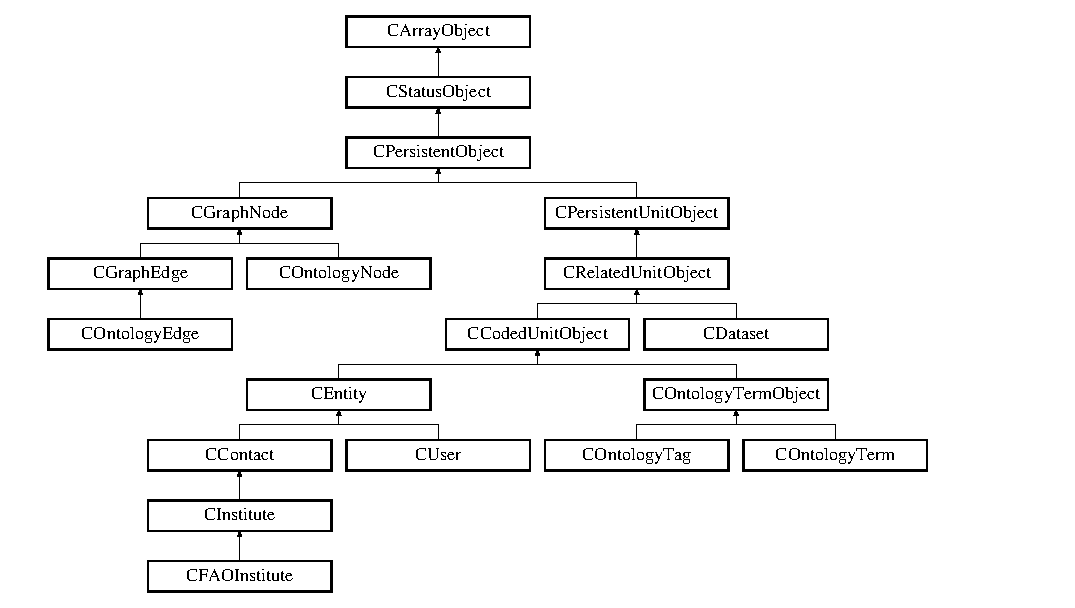
\includegraphics[height=9.655172cm]{class_c_persistent_object}
\end{center}
\end{figure}
\subsection*{Public Member Functions}
\begin{DoxyCompactItemize}
\item 
\hyperlink{class_c_persistent_object_a0f0729cfaef48bd1c98c0711c061a7d3}{\-\_\-\-\_\-construct} (\$the\-Container=N\-U\-L\-L, \$the\-Identifier=N\-U\-L\-L, \$the\-Modifiers=k\-F\-L\-A\-G\-\_\-\-D\-E\-F\-A\-U\-L\-T)
\item 
\hyperlink{class_c_persistent_object_a88b1f2b11d3d60e0b3d33d8b0649b68a}{Commit} (\$the\-Container=N\-U\-L\-L, \$the\-Identifier=N\-U\-L\-L, \$the\-Modifiers=k\-F\-L\-A\-G\-\_\-\-P\-E\-R\-S\-I\-S\-T\-\_\-\-R\-E\-P\-L\-A\-C\-E)
\item 
\hyperlink{class_c_persistent_object_a37c897b534e88477a06ec60b89d84450}{Uncommit} ()
\end{DoxyCompactItemize}
\subsection*{Protected Member Functions}
\begin{DoxyCompactItemize}
\item 
\hyperlink{class_c_persistent_object_a6520a7bcecf3f39fd61ec6d08f736e77}{\-\_\-\-Is\-Committed} (\$the\-State=N\-U\-L\-L)
\item 
\hyperlink{class_c_persistent_object_aa8dc7db66e2af3d28c2035161a2aabf9}{\-\_\-\-Is\-Encoded} (\$the\-State=N\-U\-L\-L)
\item 
\hyperlink{class_c_persistent_object_a584005d1ec0d7e7327dc6d267a9ec50c}{\-\_\-\-Create} (\&\$the\-Content)
\item 
\hyperlink{class_c_persistent_object_ad5376e5aeda7a58e5b27fae6c03b4ef9}{\-\_\-\-Commit} (\&\$the\-Container, \&\$the\-Identifier, \&\$the\-Modifiers)
\item 
\hyperlink{class_c_persistent_object_ada4dfe5bdb0309dee9df94f6e96dc3cb}{\-\_\-\-Load} (\&\$the\-Container, \&\$the\-Identifier, \&\$the\-Modifiers)
\item 
\hyperlink{class_c_persistent_object_a2e5dd4f8a92c0ada964ade712c9579b0}{\-\_\-\-Prepare\-Create} (\&\$the\-Container, \&\$the\-Identifier, \&\$the\-Modifiers)
\item 
\hyperlink{class_c_persistent_object_a5a664513b015919da582c6f0230fab75}{\-\_\-\-Prepare\-Load} (\&\$the\-Container, \&\$the\-Identifier, \&\$the\-Modifiers)
\item 
\hyperlink{class_c_persistent_object_a9d98503112f78729b13995a850b174a8}{\-\_\-\-Prepare\-Commit} (\&\$the\-Container, \&\$the\-Identifier, \&\$the\-Modifiers)
\item 
\hyperlink{class_c_persistent_object_a9029ba173e65e2ec14eeb8bc7c2024c6}{\-\_\-\-Finish\-Create} (\&\$the\-Container)
\item 
\hyperlink{class_c_persistent_object_a35ffbe4e875e03a84985493bbce75457}{\-\_\-\-Finish\-Load} (\&\$the\-Container, \&\$the\-Identifier, \&\$the\-Modifiers)
\item 
\hyperlink{class_c_persistent_object_a535a2f078b777a144d31117de054ccf7}{\-\_\-\-Finish\-Commit} (\&\$the\-Container, \&\$the\-Identifier, \&\$the\-Modifiers)
\item 
\hyperlink{class_c_persistent_object_a948ba9d69729dfe20564aecdb9d4fae7}{\-\_\-\-Set\-Tags} (\$the\-Offset=k\-T\-A\-G\-\_\-\-T\-A\-G\-S)
\item 
\hyperlink{class_c_persistent_object_a7a9363dc8aba31cf00e382172ba327bd}{\-\_\-\-Get\-Tags} ()
\end{DoxyCompactItemize}
\subsection*{Additional Inherited Members}


\subsection{Constructor \& Destructor Documentation}
\hypertarget{class_c_persistent_object_a0f0729cfaef48bd1c98c0711c061a7d3}{\index{C\-Persistent\-Object@{C\-Persistent\-Object}!\-\_\-\-\_\-construct@{\-\_\-\-\_\-construct}}
\index{\-\_\-\-\_\-construct@{\-\_\-\-\_\-construct}!CPersistentObject@{C\-Persistent\-Object}}
\subsubsection[{\-\_\-\-\_\-construct}]{\setlength{\rightskip}{0pt plus 5cm}C\-Persistent\-Object\-::\-\_\-\-\_\-construct (
\begin{DoxyParamCaption}
\item[{}]{\$the\-Container = {\ttfamily NULL}, }
\item[{}]{\$the\-Identifier = {\ttfamily NULL}, }
\item[{}]{\$the\-Modifiers = {\ttfamily kFLAG\-\_\-DEFAULT}}
\end{DoxyParamCaption}
)}}\label{class_c_persistent_object_a0f0729cfaef48bd1c98c0711c061a7d3}
Instantiate class.

The constructor can be used to instantiate an empty object, instantiate an object from some content, or load an object from a container.

The parameters to this method are\-:


\begin{DoxyItemize}
\item {\bfseries \$the\-Container}\-: This parameter represents either the {\itshape contents} of the object, if the next parameter is missing, or the {\itshape \hyperlink{class_c_container}{container}} in which the object resides. If missing, we assume we want to create an empty object. 
\begin{DoxyItemize}
\item {\itshape N\-U\-L\-L}\-: In this case it is assumed you want to instantiate an empty object and the next parameter will be ignored. 
\item {\itshape Array} or {\itshape Array\-Object}\-: In this case we assume the parameter represents either the object contents, if the next parameter is {\itshape N\-U\-L\-L}, or the \hyperlink{class_c_container}{container} in which the object is \hyperlink{class_c_persistent_object_a88b1f2b11d3d60e0b3d33d8b0649b68a}{stored}, in which case we interpret the next parameter to be the object's identifier. 
\item {\itshape Other}\-: Any other type will raise an \hyperlink{}{exception}, or it should be handled by derived classes. 
\end{DoxyItemize}
\item {\bfseries \$the\-Identifier}\-: This parameter represents the key or query that will be used to locate the object in the container provided in the first parameter. 
\begin{DoxyItemize}
\item {\itshape N\-U\-L\-L}\-: This indicates that the first parameter represents the object {\itshape contents}. 
\item {\itshape other}\-: Any other type is considered as a key or query used to locate the object in the container provided in the first parameter. 
\end{DoxyItemize}
\item {\bfseries \$the\-Modifiers}\-: This bitfield parameter can be used to provide a series of options to the object. The available options can be consulted in \hyperlink{}{this} file. Most of these options are managed automatically and should not be provided explicitly. This class handles one option that has the following meaning\-: 
\begin{DoxyItemize}
\item {\itshape \hyperlink{}{k\-F\-L\-A\-G\-\_\-\-S\-T\-A\-T\-E\-\_\-\-E\-N\-C\-O\-D\-E\-D}}\-: If the option is on, the object will be passed through a \hyperlink{class_c_container_aa339d3c4c9b011713176a89fe9c7783d}{conversion} process that will convert all \hyperlink{class_c_data_type}{standard} data types into native container custom data types \hyperlink{class_c_container_a0dc47e54abc533cedf1c2c0f915d96b2}{before} \hyperlink{class_c_persistent_object_a88b1f2b11d3d60e0b3d33d8b0649b68a}{committing} the object; the opposite \hyperlink{class_c_data_type_a608d6fc184bce537ce83669f729d6008}{conversion} process will take place \hyperlink{class_c_container_ab53bd683f0e28b2203897cf03f9d1c76}{after} \hyperlink{class_c_persistent_object_a0f0729cfaef48bd1c98c0711c061a7d3}{loading} the object from a container. It is a good idea to keep this flag O\-N, because the converted object will be compatible with any \hyperlink{class_c_container}{container} and it will make data transfers from one database to the other easy. This process is automatic and transparent. 
\end{DoxyItemize}
\end{DoxyItemize}

Depending on the results of this method we set the \hyperlink{class_c_persistent_object_a6520a7bcecf3f39fd61ec6d08f736e77}{committed} status \hyperlink{}{flag} as follows\-:


\begin{DoxyItemize}
\item {\itshape Empty object}\-: By omitting the first parameter we indicate that we want to start from scratch, the object will not have its \hyperlink{class_c_persistent_object_a6520a7bcecf3f39fd61ec6d08f736e77}{committed} \hyperlink{}{flag} set. 
\item {\itshape Filled object}\-: In this case we provide in the {\itshape \$the\-Container} parameter the object's {\itshape contents}. In this case we do not consider the object as persistent, so the object will not have its \hyperlink{class_c_persistent_object_a6520a7bcecf3f39fd61ec6d08f736e77}{committed} \hyperlink{}{flag} set. 
\item {\itshape Selected object}\-: In this case we search the {\itshape \$the\-Container} with the provided {\itshape \$the\-Identifier} as a key or query, and if\-: 
\begin{DoxyItemize}
\item {\itshape Found}\-: We set the \hyperlink{class_c_persistent_object_a6520a7bcecf3f39fd61ec6d08f736e77}{committed} \hyperlink{}{flag} on. 
\item {\itshape Not found}\-: We instantiate an empty object and ignore the \hyperlink{class_c_persistent_object_a6520a7bcecf3f39fd61ec6d08f736e77}{committed} \hyperlink{}{flag}. 
\end{DoxyItemize}
\end{DoxyItemize}

The \hyperlink{class_c_status_object_a8429102e4f52f7558649b64f4e673a69}{inited} status \hyperlink{}{flag} is not set by default, this will prevent the object from being \hyperlink{class_c_persistent_object_a88b1f2b11d3d60e0b3d33d8b0649b68a}{stored} and it is the responsibility of derived concrete instances to manage this status.

This method takes advantage of a protected interface which should be overloaded by derived classes instead of overloading this method\-:


\begin{DoxyItemize}
\item {\itshape Retrieve object}\-: If the second parameter was provided, it implies that the object is to be retrieved from the first parameter which represents the \hyperlink{class_c_container}{container} in which the object contents are stored. 
\begin{DoxyItemize}
\item {\itshape \hyperlink{class_c_persistent_object_a5a664513b015919da582c6f0230fab75}{\-\_\-\-Prepare\-Load}()}\-: This method should check and normalise the container and identifier. In this class we ensure that the container is derived from \hyperlink{class_c_container}{C\-Container}. 
\item {\itshape \hyperlink{class_c_persistent_object_ada4dfe5bdb0309dee9df94f6e96dc3cb}{\-\_\-\-Load}()}\-: This method will delegate the \hyperlink{class_c_container}{container} the responsibility of locating and retrieving the object using the provided identifier. 
\end{DoxyItemize}
\item {\itshape \hyperlink{class_c_persistent_object_a584005d1ec0d7e7327dc6d267a9ec50c}{\-\_\-\-Create}()}\-: This method should instantiate the object from the contents returned by \hyperlink{class_c_persistent_object_ada4dfe5bdb0309dee9df94f6e96dc3cb}{\-\_\-\-Load} or by the data provided in the first parameter in the case the second parameter was omitted. 
\end{DoxyItemize}

Derived classes should overload the above interface rather than overloading this method and should do so only if necessary, because this workflow should be sufficient for persisting objects.


\begin{DoxyParams}[1]{Parameters}
mixed & {\em \$the\-Container} & Persistent container. \\
\hline
mixed & {\em \$the\-Identifier} & Object identifier. \\
\hline
bitfield & {\em \$the\-Modifiers} & Create modifiers.\\
\hline
\end{DoxyParams}
public

\hyperlink{class_c_persistent_object_a5a664513b015919da582c6f0230fab75}{\-\_\-\-Prepare\-Load()}  \hyperlink{class_c_persistent_object_ada4dfe5bdb0309dee9df94f6e96dc3cb}{\-\_\-\-Load()}  \hyperlink{class_c_persistent_object_a584005d1ec0d7e7327dc6d267a9ec50c}{\-\_\-\-Create()}  \hyperlink{class_c_persistent_object_a6520a7bcecf3f39fd61ec6d08f736e77}{\-\_\-\-Is\-Committed()}  \hyperlink{class_c_persistent_object_a35ffbe4e875e03a84985493bbce75457}{\-\_\-\-Finish\-Load()}  \hyperlink{class_c_persistent_object_a9029ba173e65e2ec14eeb8bc7c2024c6}{\-\_\-\-Finish\-Create()} 

Reimplemented in \hyperlink{class_c_user_af83ffccb40893a43d90eafe396cbdec1}{C\-User}, \hyperlink{class_c_institute_a468ba723fabd5a67bea5016d1531b147}{C\-Institute}, \hyperlink{class_c_ontology_term_a33679101b2a63044f0084918a8df123e}{C\-Ontology\-Term}, \hyperlink{class_c_coded_unit_object_a314fc62af62314f5ac5acca2ac809900}{C\-Coded\-Unit\-Object}, and \hyperlink{class_c_ontology_term_object_af1fb502088538ad7372719c20f73bc5c}{C\-Ontology\-Term\-Object}.



\subsection{Member Function Documentation}
\hypertarget{class_c_persistent_object_ad5376e5aeda7a58e5b27fae6c03b4ef9}{\index{C\-Persistent\-Object@{C\-Persistent\-Object}!\-\_\-\-Commit@{\-\_\-\-Commit}}
\index{\-\_\-\-Commit@{\-\_\-\-Commit}!CPersistentObject@{C\-Persistent\-Object}}
\subsubsection[{\-\_\-\-Commit}]{\setlength{\rightskip}{0pt plus 5cm}C\-Persistent\-Object\-::\-\_\-\-Commit (
\begin{DoxyParamCaption}
\item[{\&}]{\$the\-Container, }
\item[{\&}]{\$the\-Identifier, }
\item[{\&}]{\$the\-Modifiers}
\end{DoxyParamCaption}
)\hspace{0.3cm}{\ttfamily [protected]}}}\label{class_c_persistent_object_ad5376e5aeda7a58e5b27fae6c03b4ef9}
Store object in container.

The duty of this method is to store the current object in the container provided in the first parameter with as key the value provided in the second parameter with options provided in the third parameter, please refer to \hyperlink{class_c_persistent_object_a88b1f2b11d3d60e0b3d33d8b0649b68a}{this} documentation for a reference of these parameters. Note that in this method all three parameters are passed by reference.

This class supports \hyperlink{class_c_container}{C\-Container} derived instances and will delegate the operation to the container. Note that by default we call the container's \hyperlink{class_c_container_a4847dc676d1f7704e75f8981e927508a}{commit} method with the \hyperlink{}{k\-F\-L\-A\-G\-\_\-\-P\-E\-R\-S\-I\-S\-T\-\_\-\-R\-E\-P\-L\-A\-C\-E} option, which will \hyperlink{}{insert} the object if new or \hyperlink{}{replace} the eventual existing object.

The method expects all parameters to have been previously \hyperlink{class_c_persistent_object_a9d98503112f78729b13995a850b174a8}{checked}, its main duty is to perform the actual storage. In derived classes you should intercept custom containers, or call the parent method.

{\itshape Note\-: the duty of this method is to store only the array part of the object, properties should be ignored.}


\begin{DoxyParams}[1]{Parameters}
reference & {\em \&\$the\-Container} & Object container. \\
\hline
reference & {\em \&\$the\-Identifier} & Object identifier. \\
\hline
reference & {\em \&\$the\-Modifiers} & Commit modifiers.\\
\hline
\end{DoxyParams}
protected \begin{DoxyReturn}{Returns}
mixed 
\end{DoxyReturn}


Reimplemented in \hyperlink{class_c_ontology_node_a590c869a08d167ba35d987e450106a2d}{C\-Ontology\-Node}, \hyperlink{class_c_graph_node_a7af17771eaba24551f8c9a465f391c23}{C\-Graph\-Node}, \hyperlink{class_c_persistent_unit_object_ae8726af138967ed9b4b2edbfa2a188a3}{C\-Persistent\-Unit\-Object}, \hyperlink{class_c_ontology_edge_a76e551f21dcac3c0bc228c67226bec08}{C\-Ontology\-Edge}, and \hyperlink{class_c_graph_edge_a73dd2ced3103285f8ad4ea212c0e918e}{C\-Graph\-Edge}.

\hypertarget{class_c_persistent_object_a584005d1ec0d7e7327dc6d267a9ec50c}{\index{C\-Persistent\-Object@{C\-Persistent\-Object}!\-\_\-\-Create@{\-\_\-\-Create}}
\index{\-\_\-\-Create@{\-\_\-\-Create}!CPersistentObject@{C\-Persistent\-Object}}
\subsubsection[{\-\_\-\-Create}]{\setlength{\rightskip}{0pt plus 5cm}C\-Persistent\-Object\-::\-\_\-\-Create (
\begin{DoxyParamCaption}
\item[{\&}]{\$the\-Content}
\end{DoxyParamCaption}
)\hspace{0.3cm}{\ttfamily [protected]}}}\label{class_c_persistent_object_a584005d1ec0d7e7327dc6d267a9ec50c}
Create object.

The duty of this method is to instantiate an object with the provided data.

The method expects one parameter which is passed by reference\-:


\begin{DoxyItemize}
\item {\bfseries \&\$the\-Content}\-: This parameter represents the object contents\-: 
\begin{DoxyItemize}
\item {\itshape N\-U\-L\-L}\-: The method will instantiate an empty object. 
\item {\itshape array} or an {\itshape Array\-Object}\-: The method will instantiate the object with the contents of the provided parameter. 
\item {\itshape other}\-: By default any other type will raise an exception, in derived classes you can overload this method to handle custom types. 
\end{DoxyItemize}
\end{DoxyItemize}

The method returns a boolean where {\itshape T\-R\-U\-E} indicates that the object was instantiated with data, and {\itshape F\-A\-L\-S\-E} indicating that the object is empty. This will be used by the \hyperlink{class_c_persistent_object_a0f0729cfaef48bd1c98c0711c061a7d3}{caller} to set the object \hyperlink{class_c_persistent_object_a6520a7bcecf3f39fd61ec6d08f736e77}{committed} status \hyperlink{}{flag}.

The parameter is provided as a reference.


\begin{DoxyParams}[1]{Parameters}
reference & {\em \&\$the\-Content} & Object data content.\\
\hline
\end{DoxyParams}
protected \begin{DoxyReturn}{Returns}
boolean
\end{DoxyReturn}

\begin{DoxyExceptions}{Exceptions}
{\em \{@link} & \hyperlink{class_c_exception}{C\-Exception} \hyperlink{class_c_exception}{C\-Exception}\}\\
\hline
\end{DoxyExceptions}
\begin{DoxySeeAlso}{See also}
k\-E\-R\-R\-O\-R\-\_\-\-U\-N\-S\-U\-P\-P\-O\-R\-T\-E\-D 
\end{DoxySeeAlso}


Reimplemented in \hyperlink{class_c_graph_node_a90e49bf5e95ccf3c8644196696154268}{C\-Graph\-Node}.

\hypertarget{class_c_persistent_object_a535a2f078b777a144d31117de054ccf7}{\index{C\-Persistent\-Object@{C\-Persistent\-Object}!\-\_\-\-Finish\-Commit@{\-\_\-\-Finish\-Commit}}
\index{\-\_\-\-Finish\-Commit@{\-\_\-\-Finish\-Commit}!CPersistentObject@{C\-Persistent\-Object}}
\subsubsection[{\-\_\-\-Finish\-Commit}]{\setlength{\rightskip}{0pt plus 5cm}C\-Persistent\-Object\-::\-\_\-\-Finish\-Commit (
\begin{DoxyParamCaption}
\item[{\&}]{\$the\-Container, }
\item[{\&}]{\$the\-Identifier, }
\item[{\&}]{\$the\-Modifiers}
\end{DoxyParamCaption}
)\hspace{0.3cm}{\ttfamily [protected]}}}\label{class_c_persistent_object_a535a2f078b777a144d31117de054ccf7}
Normalise after a \hyperlink{class_c_persistent_object_ad5376e5aeda7a58e5b27fae6c03b4ef9}{commit}.

This method will be called after the \hyperlink{class_c_persistent_object_ad5376e5aeda7a58e5b27fae6c03b4ef9}{store} operation, its duty is to clean up or restore the object after the operation please refer to \hyperlink{class_c_persistent_object_a88b1f2b11d3d60e0b3d33d8b0649b68a}{this} documentation for a reference of these parameters. Note that in this method all three parameters are passed by reference.

In this class we set the \hyperlink{class_c_persistent_object_a6520a7bcecf3f39fd61ec6d08f736e77}{commit} \hyperlink{}{flag} and reset the \hyperlink{class_c_status_object_a19c4ac94dfe26476e780d77b99744d43}{dirty} \hyperlink{}{flag}.


\begin{DoxyParams}[1]{Parameters}
reference & {\em \&\$the\-Container} & Object container. \\
\hline
reference & {\em \&\$the\-Identifier} & Object identifier. \\
\hline
reference & {\em \&\$the\-Modifiers} & Commit modifiers.\\
\hline
\end{DoxyParams}
protected \hypertarget{class_c_persistent_object_a9029ba173e65e2ec14eeb8bc7c2024c6}{\index{C\-Persistent\-Object@{C\-Persistent\-Object}!\-\_\-\-Finish\-Create@{\-\_\-\-Finish\-Create}}
\index{\-\_\-\-Finish\-Create@{\-\_\-\-Finish\-Create}!CPersistentObject@{C\-Persistent\-Object}}
\subsubsection[{\-\_\-\-Finish\-Create}]{\setlength{\rightskip}{0pt plus 5cm}C\-Persistent\-Object\-::\-\_\-\-Finish\-Create (
\begin{DoxyParamCaption}
\item[{\&}]{\$the\-Container}
\end{DoxyParamCaption}
)\hspace{0.3cm}{\ttfamily [protected]}}}\label{class_c_persistent_object_a9029ba173e65e2ec14eeb8bc7c2024c6}
Normalise after a \hyperlink{class_c_persistent_object_a584005d1ec0d7e7327dc6d267a9ec50c}{create}.

This method will be called after the \hyperlink{class_c_persistent_object_a584005d1ec0d7e7327dc6d267a9ec50c}{create} operation, its duty is to initialise an empty object. Both the container and the identifier parameters are passed by reference.

This method will be called if the identifier was not provided to the \hyperlink{class_c_persistent_object_a0f0729cfaef48bd1c98c0711c061a7d3}{constructor}, or if the \hyperlink{class_c_persistent_object_a0f0729cfaef48bd1c98c0711c061a7d3}{constructor} was unable to \hyperlink{class_c_persistent_object_ada4dfe5bdb0309dee9df94f6e96dc3cb}{find} the requested object.

In this class we do nothing.


\begin{DoxyParams}[1]{Parameters}
reference & {\em \&\$the\-Container} & Object container.\\
\hline
\end{DoxyParams}
protected 

Reimplemented in \hyperlink{class_c_ontology_node_a3f116a2f1a1047da5187f21e20d3d405}{C\-Ontology\-Node}, \hyperlink{class_c_graph_node_a8a8df45cff2375d0bcbb15342ae3960b}{C\-Graph\-Node}, \hyperlink{class_c_ontology_edge_a0956d5920484a329c77d878bb6c25784}{C\-Ontology\-Edge}, and \hyperlink{class_c_graph_edge_a42fd83eff1eef079a6005e961fd2d371}{C\-Graph\-Edge}.

\hypertarget{class_c_persistent_object_a35ffbe4e875e03a84985493bbce75457}{\index{C\-Persistent\-Object@{C\-Persistent\-Object}!\-\_\-\-Finish\-Load@{\-\_\-\-Finish\-Load}}
\index{\-\_\-\-Finish\-Load@{\-\_\-\-Finish\-Load}!CPersistentObject@{C\-Persistent\-Object}}
\subsubsection[{\-\_\-\-Finish\-Load}]{\setlength{\rightskip}{0pt plus 5cm}C\-Persistent\-Object\-::\-\_\-\-Finish\-Load (
\begin{DoxyParamCaption}
\item[{\&}]{\$the\-Container, }
\item[{\&}]{\$the\-Identifier, }
\item[{\&}]{\$the\-Modifiers}
\end{DoxyParamCaption}
)\hspace{0.3cm}{\ttfamily [protected]}}}\label{class_c_persistent_object_a35ffbe4e875e03a84985493bbce75457}
Normalise after a \hyperlink{class_c_persistent_object_ada4dfe5bdb0309dee9df94f6e96dc3cb}{load}.

This method will be called after the \hyperlink{class_c_persistent_object_ada4dfe5bdb0309dee9df94f6e96dc3cb}{load} operation, its duty is to clean up or normalise after the operation. Both the container and the identifier parameters are passed by reference.

In this class we do nothing.


\begin{DoxyParams}[1]{Parameters}
reference & {\em \&\$the\-Container} & Object container. \\
\hline
reference & {\em \&\$the\-Identifier} & Object identifier. \\
\hline
reference & {\em \&\$the\-Modifiers} & Create modifiers.\\
\hline
\end{DoxyParams}
protected 

Reimplemented in \hyperlink{class_c_ontology_node_a97c5e875641e3bb3da83d32ed8b26ebc}{C\-Ontology\-Node}, \hyperlink{class_c_graph_node_a23c2beb0fbed1ab67018dd9d78dee8fa}{C\-Graph\-Node}, \hyperlink{class_c_ontology_edge_ac45af3396c797be599c2a1780b7bfa59}{C\-Ontology\-Edge}, and \hyperlink{class_c_graph_edge_a7cbf3dab4745b0924905fce01e383819}{C\-Graph\-Edge}.

\hypertarget{class_c_persistent_object_a7a9363dc8aba31cf00e382172ba327bd}{\index{C\-Persistent\-Object@{C\-Persistent\-Object}!\-\_\-\-Get\-Tags@{\-\_\-\-Get\-Tags}}
\index{\-\_\-\-Get\-Tags@{\-\_\-\-Get\-Tags}!CPersistentObject@{C\-Persistent\-Object}}
\subsubsection[{\-\_\-\-Get\-Tags}]{\setlength{\rightskip}{0pt plus 5cm}C\-Persistent\-Object\-::\-\_\-\-Get\-Tags (
\begin{DoxyParamCaption}
{}
\end{DoxyParamCaption}
)\hspace{0.3cm}{\ttfamily [protected]}}}\label{class_c_persistent_object_a7a9363dc8aba31cf00e382172ba327bd}
Get attribute tags.

The duty of this method is to collect all attribute tags used in the object and return them as an array.

protected \begin{DoxyReturn}{Returns}
array 
\end{DoxyReturn}


Reimplemented in \hyperlink{class_c_persistent_unit_object_ac4df6b15733c79b93493131275a27493}{C\-Persistent\-Unit\-Object}.

\hypertarget{class_c_persistent_object_a6520a7bcecf3f39fd61ec6d08f736e77}{\index{C\-Persistent\-Object@{C\-Persistent\-Object}!\-\_\-\-Is\-Committed@{\-\_\-\-Is\-Committed}}
\index{\-\_\-\-Is\-Committed@{\-\_\-\-Is\-Committed}!CPersistentObject@{C\-Persistent\-Object}}
\subsubsection[{\-\_\-\-Is\-Committed}]{\setlength{\rightskip}{0pt plus 5cm}C\-Persistent\-Object\-::\-\_\-\-Is\-Committed (
\begin{DoxyParamCaption}
\item[{}]{\$the\-State = {\ttfamily NULL}}
\end{DoxyParamCaption}
)\hspace{0.3cm}{\ttfamily [protected]}}}\label{class_c_persistent_object_a6520a7bcecf3f39fd61ec6d08f736e77}
Manage committed status.

This method can be used to get or set the object's committed state.

A committed object is one that has either been loaded from a container or committed to a container. This state indicates that the object is persistent. This state, combined with the \hyperlink{class_c_status_object_a19c4ac94dfe26476e780d77b99744d43}{dirty} status, can determine if an object needs to be committed in a container or not.

The method features a single parameter\-:


\begin{DoxyItemize}
\item {\itshape N\-U\-L\-L}\-: The method will return {\itshape T\-R\-U\-E} if the object is committed, or {\itshape F\-A\-L\-S\-E} if the object is not committed. 
\item {\itshape T\-R\-U\-E}\-: The method will set the object to committed. 
\item {\itshape F\-A\-L\-S\-E}\-: The method will reset the object's committed state. 
\end{DoxyItemize}

In all cases the method will return the state {\itshape after} it was eventually modified.


\begin{DoxyParams}[1]{Parameters}
mixed & {\em \$the\-State} & T\-R\-U\-E, F\-A\-L\-S\-E or N\-U\-L\-L.\\
\hline
\end{DoxyParams}
protected \begin{DoxyReturn}{Returns}
boolean
\end{DoxyReturn}
\hyperlink{class_c_status_object_a3e37d72a6462d93bf7ff567f07f78093}{\-\_\-\-Manage\-Bit\-Field()}

\begin{DoxySeeAlso}{See also}
k\-F\-L\-A\-G\-\_\-\-S\-T\-A\-T\-E\-\_\-\-C\-O\-M\-M\-I\-T\-T\-E\-D 
\end{DoxySeeAlso}
\hypertarget{class_c_persistent_object_aa8dc7db66e2af3d28c2035161a2aabf9}{\index{C\-Persistent\-Object@{C\-Persistent\-Object}!\-\_\-\-Is\-Encoded@{\-\_\-\-Is\-Encoded}}
\index{\-\_\-\-Is\-Encoded@{\-\_\-\-Is\-Encoded}!CPersistentObject@{C\-Persistent\-Object}}
\subsubsection[{\-\_\-\-Is\-Encoded}]{\setlength{\rightskip}{0pt plus 5cm}C\-Persistent\-Object\-::\-\_\-\-Is\-Encoded (
\begin{DoxyParamCaption}
\item[{}]{\$the\-State = {\ttfamily NULL}}
\end{DoxyParamCaption}
)\hspace{0.3cm}{\ttfamily [protected]}}}\label{class_c_persistent_object_aa8dc7db66e2af3d28c2035161a2aabf9}
Manage encoded status.

This method can be used to get or set the object's encoded state.

This flag determines whether custom data types are to be converted to \hyperlink{class_c_data_type}{standard} types when working with the object. This is especially useful when transmitting the object through the network or when managing custom database types.

The conversion to \hyperlink{class_c_data_type}{standard} types is \hyperlink{class_c_data_type_a608d6fc184bce537ce83669f729d6008}{done} when \hyperlink{class_c_persistent_object_a0f0729cfaef48bd1c98c0711c061a7d3}{loading} the object from a \hyperlink{class_c_container}{container} and the opposite is \hyperlink{class_c_container_aa339d3c4c9b011713176a89fe9c7783d}{done} before \hyperlink{class_c_persistent_object_a88b1f2b11d3d60e0b3d33d8b0649b68a}{storing} the object into a \hyperlink{class_c_container}{container}, these operations are performed by the \hyperlink{class_c_container}{container} object that takes care of object persistence.

This \hyperlink{}{k\-F\-L\-A\-G\-\_\-\-S\-T\-A\-T\-E\-\_\-\-E\-N\-C\-O\-D\-E\-D} flag can be provided at \hyperlink{class_c_persistent_object_a0f0729cfaef48bd1c98c0711c061a7d3}{instantiation} or directly to the persistence methods, although it is a better idea to provide it in the \hyperlink{class_c_persistent_object_a0f0729cfaef48bd1c98c0711c061a7d3}{constructor} to have this conversion happen transparently.

The method features a single parameter\-:


\begin{DoxyItemize}
\item {\itshape N\-U\-L\-L}\-: The method will return {\itshape T\-R\-U\-E} if the object is encoded, or {\itshape F\-A\-L\-S\-E} if the object is not encoded. 
\item {\itshape T\-R\-U\-E}\-: The method will set the object to encoded. 
\item {\itshape F\-A\-L\-S\-E}\-: The method will reset the object's encoded state. 
\end{DoxyItemize}

In all cases the method will return the state {\itshape after} it was eventually modified.


\begin{DoxyParams}[1]{Parameters}
mixed & {\em \$the\-State} & T\-R\-U\-E, F\-A\-L\-S\-E or N\-U\-L\-L.\\
\hline
\end{DoxyParams}
protected \begin{DoxyReturn}{Returns}
boolean
\end{DoxyReturn}
\hyperlink{class_c_status_object_a3e37d72a6462d93bf7ff567f07f78093}{\-\_\-\-Manage\-Bit\-Field()}

\begin{DoxySeeAlso}{See also}
k\-F\-L\-A\-G\-\_\-\-S\-T\-A\-T\-E\-\_\-\-E\-N\-C\-O\-D\-E\-D 
\end{DoxySeeAlso}
\hypertarget{class_c_persistent_object_ada4dfe5bdb0309dee9df94f6e96dc3cb}{\index{C\-Persistent\-Object@{C\-Persistent\-Object}!\-\_\-\-Load@{\-\_\-\-Load}}
\index{\-\_\-\-Load@{\-\_\-\-Load}!CPersistentObject@{C\-Persistent\-Object}}
\subsubsection[{\-\_\-\-Load}]{\setlength{\rightskip}{0pt plus 5cm}C\-Persistent\-Object\-::\-\_\-\-Load (
\begin{DoxyParamCaption}
\item[{\&}]{\$the\-Container, }
\item[{\&}]{\$the\-Identifier, }
\item[{\&}]{\$the\-Modifiers}
\end{DoxyParamCaption}
)\hspace{0.3cm}{\ttfamily [protected]}}}\label{class_c_persistent_object_ada4dfe5bdb0309dee9df94f6e96dc3cb}
Find object.

The duty of this method is to locate the object identified by {\itshape \$the\-Identifier} in the container {\itshape \$the\-Container} and return its contents or {\itshape N\-U\-L\-L} if not found.

The method should expect both parameters to have been previously checked\-: in this class, the container must be an {\itshape Array\-Object} representing either the actual container, or a \hyperlink{class_c_container}{C\-Container} derived instance which will take care of locating the object within its managed native container.


\begin{DoxyParams}[1]{Parameters}
reference & {\em \&\$the\-Container} & Object container. \\
\hline
reference & {\em \&\$the\-Identifier} & Object identifier. \\
\hline
reference & {\em \&\$the\-Modifiers} & Create options.\\
\hline
\end{DoxyParams}
protected \begin{DoxyReturn}{Returns}
mixed 
\end{DoxyReturn}


Reimplemented in \hyperlink{class_c_ontology_node_a7a8304ab0e782d621012edddd8e7da3a}{C\-Ontology\-Node}, \hyperlink{class_c_graph_node_a60c57e754245042fe04dad8fb63a5fec}{C\-Graph\-Node}, \hyperlink{class_c_ontology_edge_ae7a4861887c1a73dcdbd0285cdba1d8d}{C\-Ontology\-Edge}, and \hyperlink{class_c_graph_edge_a8c19599c8543c9c1a25b9c2dfba8e223}{C\-Graph\-Edge}.

\hypertarget{class_c_persistent_object_a9d98503112f78729b13995a850b174a8}{\index{C\-Persistent\-Object@{C\-Persistent\-Object}!\-\_\-\-Prepare\-Commit@{\-\_\-\-Prepare\-Commit}}
\index{\-\_\-\-Prepare\-Commit@{\-\_\-\-Prepare\-Commit}!CPersistentObject@{C\-Persistent\-Object}}
\subsubsection[{\-\_\-\-Prepare\-Commit}]{\setlength{\rightskip}{0pt plus 5cm}C\-Persistent\-Object\-::\-\_\-\-Prepare\-Commit (
\begin{DoxyParamCaption}
\item[{\&}]{\$the\-Container, }
\item[{\&}]{\$the\-Identifier, }
\item[{\&}]{\$the\-Modifiers}
\end{DoxyParamCaption}
)\hspace{0.3cm}{\ttfamily [protected]}}}\label{class_c_persistent_object_a9d98503112f78729b13995a850b174a8}
Normalise before a store.

This method will be called before the \hyperlink{class_c_persistent_object_ad5376e5aeda7a58e5b27fae6c03b4ef9}{store} operation, its duty is to prepare the object and check the parameters for the \hyperlink{class_c_persistent_object_ad5376e5aeda7a58e5b27fae6c03b4ef9}{commit} operation, please refer to \hyperlink{class_c_persistent_object_a88b1f2b11d3d60e0b3d33d8b0649b68a}{this} documentation for a reference of these parameters. Note that in this method all three parameters are passed by reference.

By default we perform the following checks\-:


\begin{DoxyItemize}
\item Ensure the container is provided. 
\item Ensure the identifier is provided if \hyperlink{}{updating}. 
\item Ensure the object is \hyperlink{class_c_status_object_a8429102e4f52f7558649b64f4e673a69}{initialised}. 
\end{DoxyItemize}

In derived classes you should handle your custom containers or delegate to the parent method.

In this class we do not check the identifier.

Any errors should raise an exception.


\begin{DoxyParams}[1]{Parameters}
reference & {\em \&\$the\-Container} & Object container. \\
\hline
reference & {\em \&\$the\-Identifier} & Object identifier. \\
\hline
reference & {\em \&\$the\-Modifiers} & Commit modifiers.\\
\hline
\end{DoxyParams}
protected


\begin{DoxyExceptions}{Exceptions}
{\em \{@link} & \hyperlink{class_c_exception}{C\-Exception} \hyperlink{class_c_exception}{C\-Exception}\}\\
\hline
\end{DoxyExceptions}
\hyperlink{class_c_status_object_a8429102e4f52f7558649b64f4e673a69}{\-\_\-\-Is\-Inited()}

\begin{DoxySeeAlso}{See also}
k\-E\-R\-R\-O\-R\-\_\-\-I\-N\-V\-A\-L\-I\-D\-\_\-\-S\-T\-A\-T\-E k\-E\-R\-R\-O\-R\-\_\-\-O\-P\-T\-I\-O\-N\-\_\-\-M\-I\-S\-S\-I\-N\-G k\-E\-R\-R\-O\-R\-\_\-\-U\-N\-S\-U\-P\-P\-O\-R\-T\-E\-D 
\end{DoxySeeAlso}


Reimplemented in \hyperlink{class_c_ontology_node_a460df05b73fd4160e7a652ed3b03dd78}{C\-Ontology\-Node}, \hyperlink{class_c_graph_node_ad55d35f1ac947bae32fe8019daf05112}{C\-Graph\-Node}, \hyperlink{class_c_ontology_edge_a2bea996dff6e836069d75572f9386039}{C\-Ontology\-Edge}, \hyperlink{class_c_persistent_unit_object_aaa69a5dd56c441027197d5cb677972ad}{C\-Persistent\-Unit\-Object}, \hyperlink{class_c_f_a_o_institute_a9917150b0e31b741aa10c9443e880746}{C\-F\-A\-O\-Institute}, \hyperlink{class_c_ontology_term_a5d10f6baf1e484591d1d99b325e22d89}{C\-Ontology\-Term}, \hyperlink{class_c_ontology_term_object_aca3572974abb180f507fc63264a9ba15}{C\-Ontology\-Term\-Object}, \hyperlink{class_c_related_unit_object_a577c73999830641e07440126a3252286}{C\-Related\-Unit\-Object}, \hyperlink{class_c_institute_a096aa38309ae2f88250700d5755a18a6}{C\-Institute}, \hyperlink{class_c_user_aacdc43c5a38cb6b013ee9ce686b186e9}{C\-User}, and \hyperlink{class_c_entity_ac306808f0f8404fa405674cbe14fd441}{C\-Entity}.

\hypertarget{class_c_persistent_object_a2e5dd4f8a92c0ada964ade712c9579b0}{\index{C\-Persistent\-Object@{C\-Persistent\-Object}!\-\_\-\-Prepare\-Create@{\-\_\-\-Prepare\-Create}}
\index{\-\_\-\-Prepare\-Create@{\-\_\-\-Prepare\-Create}!CPersistentObject@{C\-Persistent\-Object}}
\subsubsection[{\-\_\-\-Prepare\-Create}]{\setlength{\rightskip}{0pt plus 5cm}C\-Persistent\-Object\-::\-\_\-\-Prepare\-Create (
\begin{DoxyParamCaption}
\item[{\&}]{\$the\-Container, }
\item[{\&}]{\$the\-Identifier, }
\item[{\&}]{\$the\-Modifiers}
\end{DoxyParamCaption}
)\hspace{0.3cm}{\ttfamily [protected]}}}\label{class_c_persistent_object_a2e5dd4f8a92c0ada964ade712c9579b0}
Normalise parameters of a create.

The duty of this method is to ensure that the parameters provided to a \hyperlink{class_c_persistent_object_a584005d1ec0d7e7327dc6d267a9ec50c}{create} operation are valid.

The method has a chance to work with the container and the identifier before it is set in the object.

In this class we set the \hyperlink{class_c_persistent_object_aa8dc7db66e2af3d28c2035161a2aabf9}{encoded} status \hyperlink{}{flag} if provided among the modifiers of the operation.


\begin{DoxyParams}[1]{Parameters}
reference & {\em \&\$the\-Container} & Object container. \\
\hline
reference & {\em \&\$the\-Identifier} & Object identifier. \\
\hline
reference & {\em \&\$the\-Modifiers} & Create modifiers.\\
\hline
\end{DoxyParams}
protected

\hyperlink{class_c_persistent_object_aa8dc7db66e2af3d28c2035161a2aabf9}{\-\_\-\-Is\-Encoded()}

\begin{DoxySeeAlso}{See also}
k\-F\-L\-A\-G\-\_\-\-S\-T\-A\-T\-E\-\_\-\-E\-N\-C\-O\-D\-E\-D 
\end{DoxySeeAlso}


Reimplemented in \hyperlink{class_c_ontology_node_a8dd4c8bc984a535448618bbbba987a55}{C\-Ontology\-Node}, \hyperlink{class_c_graph_node_a500c59ddfbec7fedf8598ee5d886de67}{C\-Graph\-Node}, \hyperlink{class_c_ontology_edge_a1d09b3ef8e4ef57a072291a7c09f7371}{C\-Ontology\-Edge}, \hyperlink{class_c_ontology_term_object_a7e785a79bf4c20b094450e688e3e73cf}{C\-Ontology\-Term\-Object}, and \hyperlink{class_c_entity_a4fdef5f86472b284c53a876d72ba8b07}{C\-Entity}.

\hypertarget{class_c_persistent_object_a5a664513b015919da582c6f0230fab75}{\index{C\-Persistent\-Object@{C\-Persistent\-Object}!\-\_\-\-Prepare\-Load@{\-\_\-\-Prepare\-Load}}
\index{\-\_\-\-Prepare\-Load@{\-\_\-\-Prepare\-Load}!CPersistentObject@{C\-Persistent\-Object}}
\subsubsection[{\-\_\-\-Prepare\-Load}]{\setlength{\rightskip}{0pt plus 5cm}C\-Persistent\-Object\-::\-\_\-\-Prepare\-Load (
\begin{DoxyParamCaption}
\item[{\&}]{\$the\-Container, }
\item[{\&}]{\$the\-Identifier, }
\item[{\&}]{\$the\-Modifiers}
\end{DoxyParamCaption}
)\hspace{0.3cm}{\ttfamily [protected]}}}\label{class_c_persistent_object_a5a664513b015919da582c6f0230fab75}
Normalise parameters of a find.

The duty of this method is to ensure that the parameters provided to a \hyperlink{class_c_persistent_object_ada4dfe5bdb0309dee9df94f6e96dc3cb}{find} operation are valid.

The method should first check if the provided container is of the correct type, then it should ensure that the identifier is valid.

We know that the identifier cannot be missing, since this method is only called if the identifier was provided. We should check that the provided container is of the correct type. In derived classes you should first handle your custom types, then let the parent method handle other types.

Any errors should raise an exception.

In this class we only support \hyperlink{class_c_container}{C\-Container} containers and the identifier is not expected to be {\itshape N\-U\-L\-L}.


\begin{DoxyParams}[1]{Parameters}
reference & {\em \&\$the\-Container} & Object container. \\
\hline
reference & {\em \&\$the\-Identifier} & Object identifier. \\
\hline
reference & {\em \&\$the\-Modifiers} & Create modifiers.\\
\hline
\end{DoxyParams}
protected


\begin{DoxyExceptions}{Exceptions}
{\em \{@link} & \hyperlink{class_c_exception}{C\-Exception} \hyperlink{class_c_exception}{C\-Exception}\}\\
\hline
\end{DoxyExceptions}
\hyperlink{class_c_persistent_object_aa8dc7db66e2af3d28c2035161a2aabf9}{\-\_\-\-Is\-Encoded()}

\begin{DoxySeeAlso}{See also}
k\-E\-R\-R\-O\-R\-\_\-\-O\-P\-T\-I\-O\-N\-\_\-\-M\-I\-S\-S\-I\-N\-G k\-E\-R\-R\-O\-R\-\_\-\-U\-N\-S\-U\-P\-P\-O\-R\-T\-E\-D 
\end{DoxySeeAlso}


Reimplemented in \hyperlink{class_c_ontology_node_ac8a77d7437a9be4b4aa18626b1a9f95d}{C\-Ontology\-Node}, \hyperlink{class_c_graph_node_af9f27bcc601672903af33f33d62e7ebf}{C\-Graph\-Node}, \hyperlink{class_c_ontology_edge_a6099442ba1dca683e4832d406793b5b9}{C\-Ontology\-Edge}, and \hyperlink{class_c_persistent_unit_object_a5f41b9143a5ae8fb353989c26d4ee301}{C\-Persistent\-Unit\-Object}.

\hypertarget{class_c_persistent_object_a948ba9d69729dfe20564aecdb9d4fae7}{\index{C\-Persistent\-Object@{C\-Persistent\-Object}!\-\_\-\-Set\-Tags@{\-\_\-\-Set\-Tags}}
\index{\-\_\-\-Set\-Tags@{\-\_\-\-Set\-Tags}!CPersistentObject@{C\-Persistent\-Object}}
\subsubsection[{\-\_\-\-Set\-Tags}]{\setlength{\rightskip}{0pt plus 5cm}C\-Persistent\-Object\-::\-\_\-\-Set\-Tags (
\begin{DoxyParamCaption}
\item[{}]{\$the\-Offset = {\ttfamily kTAG\-\_\-TAGS}}
\end{DoxyParamCaption}
)\hspace{0.3cm}{\ttfamily [protected]}}}\label{class_c_persistent_object_a948ba9d69729dfe20564aecdb9d4fae7}
Set attribute tags.

The duty of this method is to collect all attribute tags used in the object and store them as an array at the provided offset.

The method will collect all attributes, overload this method to exclude default attributes.


\begin{DoxyParams}[1]{Parameters}
string & {\em \$the\-Offset} & Offset.\\
\hline
\end{DoxyParams}
protected \hypertarget{class_c_persistent_object_a88b1f2b11d3d60e0b3d33d8b0649b68a}{\index{C\-Persistent\-Object@{C\-Persistent\-Object}!Commit@{Commit}}
\index{Commit@{Commit}!CPersistentObject@{C\-Persistent\-Object}}
\subsubsection[{Commit}]{\setlength{\rightskip}{0pt plus 5cm}C\-Persistent\-Object\-::\-Commit (
\begin{DoxyParamCaption}
\item[{}]{\$the\-Container = {\ttfamily NULL}, }
\item[{}]{\$the\-Identifier = {\ttfamily NULL}, }
\item[{}]{\$the\-Modifiers = {\ttfamily kFLAG\-\_\-PERSIST\-\_\-REPLACE}}
\end{DoxyParamCaption}
)}}\label{class_c_persistent_object_a88b1f2b11d3d60e0b3d33d8b0649b68a}
Commit the object into a container.

This method should be used to commit the object to a container, the method accepts two parameters\-:


\begin{DoxyItemize}
\item {\bfseries \$the\-Container}\-: This parameter represents the {\itshape container} in which the object is to be stored. By default we enforce concrete instances of \hyperlink{class_c_container}{C\-Container}, derived classes may overload the protected interface to initialise this value. 
\item {\bfseries \$the\-Identifier}\-: This parameter represents the value by which the current object will be uniquely identified in the first parameter. By default this value is required, derived classes may overload the protected interface to initialise this value. 
\item {\bfseries \$the\-Modifiers}\-: This parameter represents the commit operation options, by default we assume you want to \hyperlink{}{replace} an object, but you may change this value if you want to perform specific commit operations\-: 
\begin{DoxyItemize}
\item {\itshape \hyperlink{}{k\-F\-L\-A\-G\-\_\-\-P\-E\-R\-S\-I\-S\-T\-\_\-\-I\-N\-S\-E\-R\-T}}\-: The provided object will be inserted in the container, it is assumed that no other element in the container shares the same identifier, in that case the container \hyperlink{class_c_container_a4847dc676d1f7704e75f8981e927508a}{method} must raise an \hyperlink{}{exception}. 
\item {\itshape \hyperlink{}{k\-F\-L\-A\-G\-\_\-\-P\-E\-R\-S\-I\-S\-T\-\_\-\-U\-P\-D\-A\-T\-E}}\-: The provided object will replace the existing object. In this case the method expects the container to have an entry with the same key as the provided identifier, if this is not the case the container \hyperlink{class_c_container_a4847dc676d1f7704e75f8981e927508a}{method} must raise an \hyperlink{}{exception}. With this option it is assumed that the provided object's attributes will replace all the existing object's ones. 
\item {\itshape \hyperlink{}{k\-F\-L\-A\-G\-\_\-\-P\-E\-R\-S\-I\-S\-T\-\_\-\-M\-O\-D\-I\-F\-Y}}\-: The provided object is assumed to contain a subset of an existing object's attributes, these provided attributes will be appended or replace the existing ones. In this case the method expects the container to have an entry with the same key as the provided identifier, if this is not the case the method must raise an \hyperlink{}{exception}. 
\item {\itshape \hyperlink{}{k\-F\-L\-A\-G\-\_\-\-P\-E\-R\-S\-I\-S\-T\-\_\-\-R\-E\-P\-L\-A\-C\-E}}\-: The provided object will be \hyperlink{}{inserted}, if the identifier doesn't match any container elements, or it will \hyperlink{}{replace} the existing object. As with \hyperlink{}{update}, it is assumed that the provided object's attributes will replace all the existing object's ones. 
\item {\itshape \hyperlink{}{k\-F\-L\-A\-G\-\_\-\-P\-E\-R\-S\-I\-S\-T\-\_\-\-D\-E\-L\-E\-T\-E}}\-: This option assumes you want to remove the object from the container, although the container features a specific \hyperlink{class_c_container_aa91ec2f4624a2ebfb74668f274139329}{method} for this purpose, this option may be used to implement a {\itshape deleted state}, rather than actually removing the object from the container. 
\item {\itshape \hyperlink{}{k\-F\-L\-A\-G\-\_\-\-S\-T\-A\-T\-E\-\_\-\-E\-N\-C\-O\-D\-E\-D}}\-: If the option is on, the object will be passed through a \hyperlink{class_c_container_aa339d3c4c9b011713176a89fe9c7783d}{conversion} process that will convert all \hyperlink{class_c_data_type}{standard} data types into native container custom data types \hyperlink{class_c_container_a0dc47e54abc533cedf1c2c0f915d96b2}{before} committing the object. It is a good idea to keep this flag O\-N, because the converted object will be compatible with any \hyperlink{class_c_container}{container} and it will make data transfers from one database to the other easy. This process is automatic and transparent. 
\end{DoxyItemize}
\end{DoxyItemize}

The method will only operate if either the \hyperlink{class_c_persistent_object_a6520a7bcecf3f39fd61ec6d08f736e77}{committed} \hyperlink{}{flag} is {\itshape not set}, or the \hyperlink{class_c_status_object_a19c4ac94dfe26476e780d77b99744d43}{dirty} \hyperlink{}{flag} is {\itshape set}, if none of these two conditions are satisfied, the method will do nothing.

The method will by default {\itshape set} the \hyperlink{class_c_persistent_object_a6520a7bcecf3f39fd61ec6d08f736e77}{committed} \hyperlink{}{flag} and {\itshape reset} the \hyperlink{class_c_status_object_a19c4ac94dfe26476e780d77b99744d43}{dirty} \hyperlink{}{flag} if the operation was successful.

This method should raise an exception if any error occurs.

The method should return the unique identifier of the object or {\itshape N\-U\-L\-L} if the operation was not performed.

In derived classes you should not overload this method, instead, you should overload the protected interface\-:


\begin{DoxyItemize}
\item {\itshape \hyperlink{class_c_persistent_object_a9d98503112f78729b13995a850b174a8}{\-\_\-\-Prepare\-Commit}()}\-: This method can be used to initialise or check the parameters and resources. 
\item {\itshape \hyperlink{class_c_persistent_object_ad5376e5aeda7a58e5b27fae6c03b4ef9}{\-\_\-\-Commit}()}\-: This method will perform the actual commit. 
\item {\itshape \hyperlink{class_c_persistent_object_a535a2f078b777a144d31117de054ccf7}{\-\_\-\-Finish\-Commit}()}\-: This method can be used to perform eventual post-\/flight adjustments. 
\end{DoxyItemize}


\begin{DoxyParams}[1]{Parameters}
mixed & {\em \$the\-Container} & Persistent container. \\
\hline
mixed & {\em \$the\-Identifier} & Object identifier. \\
\hline
bitfield & {\em \$the\-Modifiers} & Commit modifiers.\\
\hline
\end{DoxyParams}
public \begin{DoxyReturn}{Returns}
mixed
\end{DoxyReturn}
\hyperlink{class_c_status_object_a19c4ac94dfe26476e780d77b99744d43}{\-\_\-\-Is\-Dirty()}  \hyperlink{class_c_persistent_object_a6520a7bcecf3f39fd61ec6d08f736e77}{\-\_\-\-Is\-Committed()}  \hyperlink{class_c_persistent_object_a9d98503112f78729b13995a850b174a8}{\-\_\-\-Prepare\-Commit()}  \hyperlink{class_c_persistent_object_ad5376e5aeda7a58e5b27fae6c03b4ef9}{\-\_\-\-Commit()}  \hyperlink{class_c_persistent_object_a535a2f078b777a144d31117de054ccf7}{\-\_\-\-Finish\-Commit()}

\begin{DoxySeeAlso}{See also}
k\-F\-L\-A\-G\-\_\-\-P\-E\-R\-S\-I\-S\-T\-\_\-\-I\-N\-S\-E\-R\-T k\-F\-L\-A\-G\-\_\-\-P\-E\-R\-S\-I\-S\-T\-\_\-\-U\-P\-D\-A\-T\-E k\-F\-L\-A\-G\-\_\-\-P\-E\-R\-S\-I\-S\-T\-\_\-\-M\-O\-D\-I\-F\-Y 

k\-F\-L\-A\-G\-\_\-\-P\-E\-R\-S\-I\-S\-T\-\_\-\-R\-E\-P\-L\-A\-C\-E k\-F\-L\-A\-G\-\_\-\-S\-T\-A\-T\-E\-\_\-\-E\-N\-C\-O\-D\-E\-D 
\end{DoxySeeAlso}
\hypertarget{class_c_persistent_object_a37c897b534e88477a06ec60b89d84450}{\index{C\-Persistent\-Object@{C\-Persistent\-Object}!Uncommit@{Uncommit}}
\index{Uncommit@{Uncommit}!CPersistentObject@{C\-Persistent\-Object}}
\subsubsection[{Uncommit}]{\setlength{\rightskip}{0pt plus 5cm}C\-Persistent\-Object\-::\-Uncommit (
\begin{DoxyParamCaption}
{}
\end{DoxyParamCaption}
)}}\label{class_c_persistent_object_a37c897b534e88477a06ec60b89d84450}
Reset \hyperlink{class_c_persistent_object_a6520a7bcecf3f39fd61ec6d08f736e77}{committed} status.

This method can be used to reset the object's \hyperlink{}{committed} \hyperlink{class_c_persistent_object_a6520a7bcecf3f39fd61ec6d08f736e77}{status}, this may be necessary when copying an object from one container to the other, since the object will be \hyperlink{class_c_persistent_object_a88b1f2b11d3d60e0b3d33d8b0649b68a}{committed} only if the \hyperlink{}{committed} \hyperlink{class_c_persistent_object_a6520a7bcecf3f39fd61ec6d08f736e77}{status} is not set, or if the \hyperlink{}{dirty} \hyperlink{class_c_status_object_a19c4ac94dfe26476e780d77b99744d43}{status} is set.

public

\hyperlink{class_c_persistent_object_a6520a7bcecf3f39fd61ec6d08f736e77}{\-\_\-\-Is\-Committed()} 

The documentation for this class was generated from the following file\-:\begin{DoxyCompactItemize}
\item 
/\-Library/\-Web\-Server/\-Library/wrapper/classes/C\-Persistent\-Object.\-php\end{DoxyCompactItemize}

\hypertarget{class_c_persistent_unit_object}{\section{C\-Persistent\-Unit\-Object Class Reference}
\label{class_c_persistent_unit_object}\index{C\-Persistent\-Unit\-Object@{C\-Persistent\-Unit\-Object}}
}
Inheritance diagram for C\-Persistent\-Unit\-Object\-:\begin{figure}[H]
\begin{center}
\leavevmode
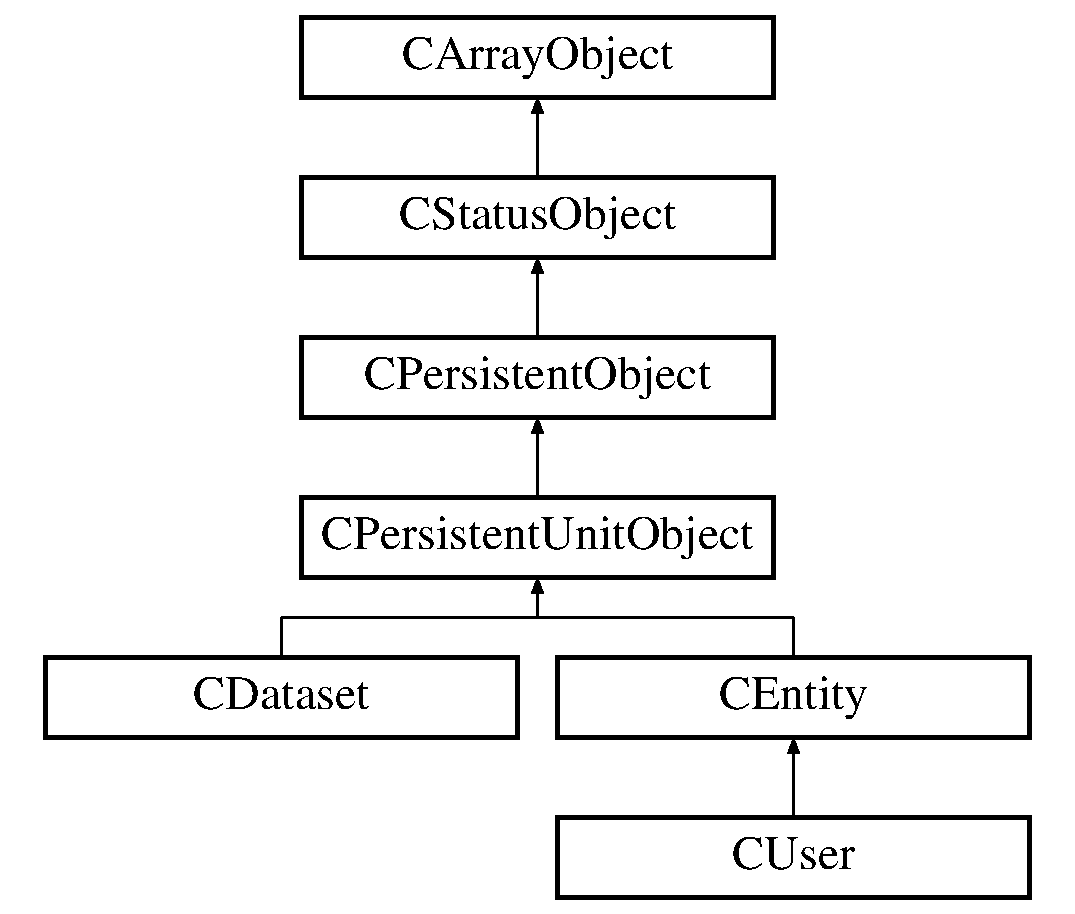
\includegraphics[height=10.000000cm]{class_c_persistent_unit_object}
\end{center}
\end{figure}
\subsection*{Public Member Functions}
\begin{DoxyCompactItemize}
\item 
\hyperlink{class_c_persistent_unit_object_af75b0a5542f5d14a9a2879e5d3864cac}{\-\_\-\-\_\-to\-String} ()
\item 
\hyperlink{class_c_persistent_unit_object_a953695de3bbfc5c3d76d0b9b3a39f6a1}{Persistent} ()
\end{DoxyCompactItemize}
\subsection*{Static Public Member Functions}
\begin{DoxyCompactItemize}
\item 
static \hyperlink{class_c_persistent_unit_object_ab3e33158e9b08a45f3a0b71feb922f50}{New\-Object} (\$the\-Container, \$the\-Identifier, \$the\-Modifiers=k\-F\-L\-A\-G\-\_\-\-D\-E\-F\-A\-U\-L\-T)
\item 
static \hyperlink{class_c_persistent_unit_object_a45700a911c2266de6e562cdd62c3c777}{Reference} (\$the\-Object, \$the\-Modifiers=k\-F\-L\-A\-G\-\_\-\-R\-E\-F\-E\-R\-E\-N\-C\-E\-\_\-\-I\-D\-E\-N\-T\-I\-F\-I\-E\-R)
\item 
static \hyperlink{class_c_persistent_unit_object_af0e75c386b883074c8bb677bac500bb3}{Hash\-Index} (\$the\-Value)
\item 
static \hyperlink{class_c_persistent_unit_object_abdf69880df0ce8257c4d0fd64adc7053}{Normalise\-Related\-Object} (\$the\-Value)
\item 
static \hyperlink{class_c_persistent_unit_object_ac7bfe8f6475e61abb2e9de9c112cbfe6}{Object\-Identifier} (\$the\-Value)
\end{DoxyCompactItemize}
\subsection*{Protected Member Functions}
\begin{DoxyCompactItemize}
\item 
\hyperlink{class_c_persistent_unit_object_ada043fb875e4ec40b6c36eef689ab2a6}{Normalise\-Related\-Predicate} (\$the\-Value)
\item 
\hyperlink{class_c_persistent_unit_object_ad1ca0920cf0df3c24351402f9afbf34b}{\-\_\-id} ()
\item 
\hyperlink{class_c_persistent_unit_object_a5166fdce0b1be6a3e4889f20c5f1c2dd}{\-\_\-index} ()
\item 
\hyperlink{class_c_persistent_unit_object_ae8726af138967ed9b4b2edbfa2a188a3}{\-\_\-\-Commit} (\&\$the\-Container, \&\$the\-Identifier, \&\$the\-Modifiers)
\item 
\hyperlink{class_c_persistent_unit_object_a5f41b9143a5ae8fb353989c26d4ee301}{\-\_\-\-Prepare\-Load} (\&\$the\-Container, \&\$the\-Identifier, \&\$the\-Modifiers)
\item 
\hyperlink{class_c_persistent_unit_object_aaa69a5dd56c441027197d5cb677972ad}{\-\_\-\-Prepare\-Commit} (\&\$the\-Container, \&\$the\-Identifier, \&\$the\-Modifiers)
\item 
\hyperlink{class_c_persistent_unit_object_ae74127a9fb936d8cf5aeed30315ac05b}{\-\_\-\-Parse\-References} (\$the\-Offset, \$the\-Container, \$the\-Modifiers=k\-F\-L\-A\-G\-\_\-\-D\-E\-F\-A\-U\-L\-T)
\item 
\hyperlink{class_c_persistent_unit_object_ac5766758d07f7ee985fd2699b8d99fce}{\-\_\-\-Commit\-References} (\&\$the\-Reference, \$the\-Container, \$the\-Modifiers, \$do\-Recurse=2)
\item 
\hyperlink{class_c_persistent_unit_object_ac4df6b15733c79b93493131275a27493}{\-\_\-\-Get\-Tags} ()
\end{DoxyCompactItemize}


\subsection{Member Function Documentation}
\hypertarget{class_c_persistent_unit_object_af75b0a5542f5d14a9a2879e5d3864cac}{\index{C\-Persistent\-Unit\-Object@{C\-Persistent\-Unit\-Object}!\-\_\-\-\_\-to\-String@{\-\_\-\-\_\-to\-String}}
\index{\-\_\-\-\_\-to\-String@{\-\_\-\-\_\-to\-String}!CPersistentUnitObject@{C\-Persistent\-Unit\-Object}}
\subsubsection[{\-\_\-\-\_\-to\-String}]{\setlength{\rightskip}{0pt plus 5cm}C\-Persistent\-Unit\-Object\-::\-\_\-\-\_\-to\-String (
\begin{DoxyParamCaption}
{}
\end{DoxyParamCaption}
)}}\label{class_c_persistent_unit_object_af75b0a5542f5d14a9a2879e5d3864cac}
Return object identifier.

In this class we return the object string \hyperlink{class_c_persistent_unit_object_a5166fdce0b1be6a3e4889f20c5f1c2dd}{identifier}.

public \begin{DoxyReturn}{Returns}
string
\end{DoxyReturn}
\hyperlink{class_c_persistent_unit_object_a5166fdce0b1be6a3e4889f20c5f1c2dd}{\-\_\-index()} \hypertarget{class_c_persistent_unit_object_ae8726af138967ed9b4b2edbfa2a188a3}{\index{C\-Persistent\-Unit\-Object@{C\-Persistent\-Unit\-Object}!\-\_\-\-Commit@{\-\_\-\-Commit}}
\index{\-\_\-\-Commit@{\-\_\-\-Commit}!CPersistentUnitObject@{C\-Persistent\-Unit\-Object}}
\subsubsection[{\-\_\-\-Commit}]{\setlength{\rightskip}{0pt plus 5cm}C\-Persistent\-Unit\-Object\-::\-\_\-\-Commit (
\begin{DoxyParamCaption}
\item[{\&}]{\$the\-Container, }
\item[{\&}]{\$the\-Identifier, }
\item[{\&}]{\$the\-Modifiers}
\end{DoxyParamCaption}
)\hspace{0.3cm}{\ttfamily [protected]}}}\label{class_c_persistent_unit_object_ae8726af138967ed9b4b2edbfa2a188a3}
Store object in container.

We overload this method to \hyperlink{class_c_persistent_unit_object_ac4df6b15733c79b93493131275a27493}{collect} and \hyperlink{class_c_persistent_object_a948ba9d69729dfe20564aecdb9d4fae7}{set} the object tags.


\begin{DoxyParams}[1]{Parameters}
reference & {\em \&\$the\-Container} & Object container. \\
\hline
reference & {\em \&\$the\-Identifier} & Object identifier. \\
\hline
reference & {\em \&\$the\-Modifiers} & Commit modifiers.\\
\hline
\end{DoxyParams}
protected \begin{DoxyReturn}{Returns}
mixed 
\end{DoxyReturn}


Reimplemented from \hyperlink{class_c_persistent_object_ad5376e5aeda7a58e5b27fae6c03b4ef9}{C\-Persistent\-Object}.

\hypertarget{class_c_persistent_unit_object_ac5766758d07f7ee985fd2699b8d99fce}{\index{C\-Persistent\-Unit\-Object@{C\-Persistent\-Unit\-Object}!\-\_\-\-Commit\-References@{\-\_\-\-Commit\-References}}
\index{\-\_\-\-Commit\-References@{\-\_\-\-Commit\-References}!CPersistentUnitObject@{C\-Persistent\-Unit\-Object}}
\subsubsection[{\-\_\-\-Commit\-References}]{\setlength{\rightskip}{0pt plus 5cm}C\-Persistent\-Unit\-Object\-::\-\_\-\-Commit\-References (
\begin{DoxyParamCaption}
\item[{\&}]{\$the\-Reference, }
\item[{}]{\$the\-Container, }
\item[{}]{\$the\-Modifiers, }
\item[{}]{\$do\-Recurse = {\ttfamily 2}}
\end{DoxyParamCaption}
)\hspace{0.3cm}{\ttfamily [protected]}}}\label{class_c_persistent_unit_object_ac5766758d07f7ee985fd2699b8d99fce}
Commit references.

This method will parse the provided value looking for object references, if such references are expressed as instances derived from this class, it will will \hyperlink{class_c_persistent_object_a88b1f2b11d3d60e0b3d33d8b0649b68a}{commit} these instances and convert them to object references.

The method will first check if the provided reference is a scalar, then it will check if it is a predicate/object par and finally it will check if it is a list of references.

The parameters to this method are\-:


\begin{DoxyItemize}
\item {\bfseries \$the\-Reference}\-: The reference to be parsed, the conversion will replace the provided parameter. 
\item {\bfseries \$the\-Container}\-: The container in which the referenced object(s) resides, please refer to the documentation of \hyperlink{class_c_persistent_unit_object_ae74127a9fb936d8cf5aeed30315ac05b}{\-\_\-\-Parse\-References} for more information. 
\item {\bfseries \$the\-Modifiers}\-: A bitfield indicating which elements of the \hyperlink{class_c_container_a1486a3cb34d24ff1c3028ad4360b5dc6}{reference} should be included, please refer to the documentation of \hyperlink{class_c_persistent_unit_object_ae74127a9fb936d8cf5aeed30315ac05b}{\-\_\-\-Parse\-References} for more information. 
\item {\bfseries \$do\-Recurse}\-: This is a private parameter that you should leave untouched, it it determines whether or not to recurse this method\-: it starts with a value of 2, and at each recursion the value decreases, when it reaches zero, structures will no more be considered. 
\end{DoxyItemize}

The method follows this set of rules\-:


\begin{DoxyItemize}
\item {\itshape Handle scalars}\-: A scalar element may be an instance derived from this class, an instance derived from \hyperlink{class_c_data_type}{C\-Data\-Type}, or anything that is not an array or an Array\-Object. If the scalar is an instance of this class, we \hyperlink{class_c_persistent_object_a88b1f2b11d3d60e0b3d33d8b0649b68a}{commit} the instance and convert it to an object reference. 
\item {\itshape Handle structures}\-: Once we have determined it is not a scalar, we check if it is either a predicate/object pair, or if it is a list of references; in the both cases the elements will be passed recursively to this method. 
\end{DoxyItemize}

Note that when we \hyperlink{class_c_persistent_object_a88b1f2b11d3d60e0b3d33d8b0649b68a}{commit} referenced objects we use \hyperlink{}{k\-F\-L\-A\-G\-\_\-\-P\-E\-R\-S\-I\-S\-T\-\_\-\-R\-E\-P\-L\-A\-C\-E} as the commit type.

The method will return {\itshape T\-R\-U\-E} is a conversion occurred and {\itshape F\-A\-L\-S\-E} if not.


\begin{DoxyParams}[1]{Parameters}
reference & {\em \&\$the\-Reference} & Reference. \\
\hline
\hyperlink{class_c_container}{C\-Container} & {\em \$the\-Container} & Object container. \\
\hline
bitfield & {\em \$the\-Modifiers} & Reference options. \\
\hline
integer & {\em \$do\-Recurse} & Recurse level.\\
\hline
\end{DoxyParams}
protected

\-\_\-\-Commit\-Reference() \hypertarget{class_c_persistent_unit_object_ac4df6b15733c79b93493131275a27493}{\index{C\-Persistent\-Unit\-Object@{C\-Persistent\-Unit\-Object}!\-\_\-\-Get\-Tags@{\-\_\-\-Get\-Tags}}
\index{\-\_\-\-Get\-Tags@{\-\_\-\-Get\-Tags}!CPersistentUnitObject@{C\-Persistent\-Unit\-Object}}
\subsubsection[{\-\_\-\-Get\-Tags}]{\setlength{\rightskip}{0pt plus 5cm}C\-Persistent\-Unit\-Object\-::\-\_\-\-Get\-Tags (
\begin{DoxyParamCaption}
{}
\end{DoxyParamCaption}
)\hspace{0.3cm}{\ttfamily [protected]}}}\label{class_c_persistent_unit_object_ac4df6b15733c79b93493131275a27493}
Get attribute tags.

In this class we exclude the \hyperlink{}{k\-T\-A\-G\-\_\-\-L\-I\-D}, \hyperlink{}{k\-T\-A\-G\-\_\-\-C\-L\-A\-S\-S} and \hyperlink{}{k\-T\-A\-G\-\_\-\-V\-E\-R\-S\-I\-O\-N} tags, since they are set by default.

protected \begin{DoxyReturn}{Returns}
array 
\end{DoxyReturn}


Reimplemented from \hyperlink{class_c_persistent_object_a7a9363dc8aba31cf00e382172ba327bd}{C\-Persistent\-Object}.

\hypertarget{class_c_persistent_unit_object_ad1ca0920cf0df3c24351402f9afbf34b}{\index{C\-Persistent\-Unit\-Object@{C\-Persistent\-Unit\-Object}!\-\_\-id@{\-\_\-id}}
\index{\-\_\-id@{\-\_\-id}!CPersistentUnitObject@{C\-Persistent\-Unit\-Object}}
\subsubsection[{\-\_\-id}]{\setlength{\rightskip}{0pt plus 5cm}C\-Persistent\-Unit\-Object\-::\-\_\-id (
\begin{DoxyParamCaption}
{}
\end{DoxyParamCaption}
)\hspace{0.3cm}{\ttfamily [protected]}}}\label{class_c_persistent_unit_object_ad1ca0920cf0df3c24351402f9afbf34b}
Return the object's unique identifier.

This method can be used to return a value that represents the object's unique native identifier. The method should use the value returned by the \hyperlink{class_c_persistent_unit_object_a5166fdce0b1be6a3e4889f20c5f1c2dd}{\-\_\-index} method and hash it if necessary.

This method will be called \hyperlink{class_c_persistent_unit_object_aaa69a5dd56c441027197d5cb677972ad}{before} \hyperlink{class_c_persistent_object_a88b1f2b11d3d60e0b3d33d8b0649b68a}{committing} the object to fill its unique identifier \hyperlink{}{offset}.

If this method returns {\itshape N\-U\-L\-L}, it is assumed that it will be the \hyperlink{class_c_container}{container} that will provide a default unique value.

In this class we return the \hyperlink{class_c_persistent_unit_object_af0e75c386b883074c8bb677bac500bb3}{hashed} value of \hyperlink{class_c_persistent_unit_object_a5166fdce0b1be6a3e4889f20c5f1c2dd}{\-\_\-index}.

protected \begin{DoxyReturn}{Returns}
mixed 
\end{DoxyReturn}
\hypertarget{class_c_persistent_unit_object_a5166fdce0b1be6a3e4889f20c5f1c2dd}{\index{C\-Persistent\-Unit\-Object@{C\-Persistent\-Unit\-Object}!\-\_\-index@{\-\_\-index}}
\index{\-\_\-index@{\-\_\-index}!CPersistentUnitObject@{C\-Persistent\-Unit\-Object}}
\subsubsection[{\-\_\-index}]{\setlength{\rightskip}{0pt plus 5cm}C\-Persistent\-Unit\-Object\-::\-\_\-index (
\begin{DoxyParamCaption}
{}
\end{DoxyParamCaption}
)\hspace{0.3cm}{\ttfamily [abstract]}, {\ttfamily [protected]}}}\label{class_c_persistent_unit_object_a5166fdce0b1be6a3e4889f20c5f1c2dd}
Return the object's unique index.

This method can be used to return a string value that represents the object's unique identifier. This value should generally be extracted from the object's properties.

In general this value will be used by the \hyperlink{class_c_persistent_unit_object_ad1ca0920cf0df3c24351402f9afbf34b}{\-\_\-id} method to form the object's unique \hyperlink{}{identifier}, maybe hashed to make the index smaller.

In this class we require derived classes to implement the method.

protected \begin{DoxyReturn}{Returns}
string 
\end{DoxyReturn}


Reimplemented in \hyperlink{class_c_term_a7524effdc0db8f5ca045f306e3b6b50e}{C\-Term}, and \hyperlink{class_c_coded_unit_object_a990c19b8bf98d2784da81e3a3121ce56}{C\-Coded\-Unit\-Object}.

\hypertarget{class_c_persistent_unit_object_ae74127a9fb936d8cf5aeed30315ac05b}{\index{C\-Persistent\-Unit\-Object@{C\-Persistent\-Unit\-Object}!\-\_\-\-Parse\-References@{\-\_\-\-Parse\-References}}
\index{\-\_\-\-Parse\-References@{\-\_\-\-Parse\-References}!CPersistentUnitObject@{C\-Persistent\-Unit\-Object}}
\subsubsection[{\-\_\-\-Parse\-References}]{\setlength{\rightskip}{0pt plus 5cm}C\-Persistent\-Unit\-Object\-::\-\_\-\-Parse\-References (
\begin{DoxyParamCaption}
\item[{}]{\$the\-Offset, }
\item[{}]{\$the\-Container, }
\item[{}]{\$the\-Modifiers = {\ttfamily kFLAG\-\_\-DEFAULT}}
\end{DoxyParamCaption}
)\hspace{0.3cm}{\ttfamily [protected]}}}\label{class_c_persistent_unit_object_ae74127a9fb936d8cf5aeed30315ac05b}
Handle references.

This method will parse the provided offset and convert all instances derived from this class to object references according to a series of rules.

Object references may have two forms\-:


\begin{DoxyItemize}
\item {\itshape Scalar}\-: A scalar value represents the object \hyperlink{}{identifier}. 
\item {\itshape Object reference structure}\-: This form is a structure holding the following elements\-: 
\begin{DoxyItemize}
\item {\itshape \hyperlink{}{k\-T\-A\-G\-\_\-\-R\-E\-F\-E\-R\-E\-N\-C\-E\-\_\-\-I\-D}}\-: This offset holds the object's \hyperlink{}{identifier}. 
\item {\itshape \hyperlink{}{k\-T\-A\-G\-\_\-\-R\-E\-F\-E\-R\-E\-N\-C\-E\-\_\-\-C\-O\-N\-T\-A\-I\-N\-E\-R}}\-: This offset holds the container name in which the object resides. 
\item {\itshape \hyperlink{}{k\-T\-A\-G\-\_\-\-R\-E\-F\-E\-R\-E\-N\-C\-E\-\_\-\-D\-A\-T\-A\-B\-A\-S\-E}}\-: This offset holds the database name in which the object resides. 
\item {\itshape \hyperlink{}{k\-T\-A\-G\-\_\-\-C\-L\-A\-S\-S}}\-: This offset holds the object's class name. 
\end{DoxyItemize}Such structures should not have any other allowed offset. 
\end{DoxyItemize}

Object references are stored in offsets with the following forms\-:


\begin{DoxyItemize}
\item {\itshape Scalar}\-: The offset holds the object reference as a scalar element. 
\item {\itshape Typed}\-: A typed object reference consists of a structure in which the \hyperlink{}{k\-T\-A\-G\-\_\-\-D\-A\-T\-A} offset holds the object reference and an optional \hyperlink{}{k\-T\-A\-G\-\_\-\-K\-I\-N\-D} offset holds the relation predicate, which may also be in the form of an object reference. 
\item {\itshape List}\-: A list of references whose elements may be a combination of the previous two formats. 
\end{DoxyItemize}

This method will pass the provided offset value to a \hyperlink{class_c_persistent_unit_object_ac5766758d07f7ee985fd2699b8d99fce}{method} that will take care of parsing the contents and \hyperlink{}{committing} all instances derived from this class into object references according to the provided modifier flags.

The parameters to this method are\-:


\begin{DoxyItemize}
\item {\bfseries \$the\-Offset}\-: The current object's offset that holds the reference or references. 
\item {\bfseries \$the\-Container}\-: The container that is about to receive the current object, it must also be the container in which to find the references and must be derived from \hyperlink{class_c_container}{C\-Container}. 
\item {\bfseries \$the\-Modifiers}\-: A bitfield indicating which elements should be included in the \hyperlink{class_c_container_a1486a3cb34d24ff1c3028ad4360b5dc6}{reference}\-: 
\begin{DoxyItemize}
\item {\itshape \hyperlink{}{k\-F\-L\-A\-G\-\_\-\-R\-E\-F\-E\-R\-E\-N\-C\-E\-\_\-\-I\-D\-E\-N\-T\-I\-F\-I\-E\-R}}\-: The object \hyperlink{}{identifier} will be stored under the \hyperlink{}{k\-T\-A\-G\-\_\-\-R\-E\-F\-E\-R\-E\-N\-C\-E\-\_\-\-I\-D} offset. This option is enforced. 
\item {\itshape \hyperlink{}{k\-F\-L\-A\-G\-\_\-\-R\-E\-F\-E\-R\-E\-N\-C\-E\-\_\-\-C\-O\-N\-T\-A\-I\-N\-E\-R}}\-: The provided container name will be stored under the \hyperlink{}{k\-T\-A\-G\-\_\-\-R\-E\-F\-E\-R\-E\-N\-C\-E\-\_\-\-C\-O\-N\-T\-A\-I\-N\-E\-R} offset. If the provided value is empty, the offset will not be set. 
\item {\itshape \hyperlink{}{k\-F\-L\-A\-G\-\_\-\-R\-E\-F\-E\-R\-E\-N\-C\-E\-\_\-\-D\-A\-T\-A\-B\-A\-S\-E}}\-: The provided container's database name will be stored under the \hyperlink{}{k\-T\-A\-G\-\_\-\-R\-E\-F\-E\-R\-E\-N\-C\-E\-\_\-\-D\-A\-T\-A\-B\-A\-S\-E} offset. If the current object's \hyperlink{}{database} name is {\itshape N\-U\-L\-L}, the offset will not be set. 
\item {\itshape \hyperlink{}{k\-F\-L\-A\-G\-\_\-\-R\-E\-F\-E\-R\-E\-N\-C\-E\-\_\-\-C\-L\-A\-S\-S}}\-: The element object's class name will be stored under the \hyperlink{}{k\-T\-A\-G\-\_\-\-C\-L\-A\-S\-S} offset. 
\end{DoxyItemize}If none of the above flags are set, it means that object references are expressed directly as the value of the \hyperlink{}{identifier}, and that \hyperlink{}{container} and \hyperlink{}{database} are implicit. 
\end{DoxyItemize}


\begin{DoxyParams}[1]{Parameters}
string & {\em \$the\-Offset} & Reference list offset. \\
\hline
\hyperlink{class_c_container}{C\-Container} & {\em \$the\-Container} & Object container. \\
\hline
bitfield & {\em \$the\-Modifiers} & Referencing options.\\
\hline
\end{DoxyParams}
protected

\-\_\-\-Commit\-Reference() \hypertarget{class_c_persistent_unit_object_aaa69a5dd56c441027197d5cb677972ad}{\index{C\-Persistent\-Unit\-Object@{C\-Persistent\-Unit\-Object}!\-\_\-\-Prepare\-Commit@{\-\_\-\-Prepare\-Commit}}
\index{\-\_\-\-Prepare\-Commit@{\-\_\-\-Prepare\-Commit}!CPersistentUnitObject@{C\-Persistent\-Unit\-Object}}
\subsubsection[{\-\_\-\-Prepare\-Commit}]{\setlength{\rightskip}{0pt plus 5cm}C\-Persistent\-Unit\-Object\-::\-\_\-\-Prepare\-Commit (
\begin{DoxyParamCaption}
\item[{\&}]{\$the\-Container, }
\item[{\&}]{\$the\-Identifier, }
\item[{\&}]{\$the\-Modifiers}
\end{DoxyParamCaption}
)\hspace{0.3cm}{\ttfamily [protected]}}}\label{class_c_persistent_unit_object_aaa69a5dd56c441027197d5cb677972ad}
Normalise before a store.

We \hyperlink{class_c_persistent_object_a9d98503112f78729b13995a850b174a8}{overload} this method to perform the following steps\-:


\begin{DoxyItemize}
\item {\itshape Identifier as structure}\-: We handle identifiers provided as object structures or references by checking the \hyperlink{}{native} identifier or the object \hyperlink{}{reference}. 
\item {\itshape Set identifier}\-: If the current object has already an \hyperlink{}{identifier} and an identifier was not provided we set it, if this is not the case we set it via the \hyperlink{class_c_persistent_unit_object_ad1ca0920cf0df3c24351402f9afbf34b}{\-\_\-id} method. 
\item {\itshape Call parent method}\-: We then call the parent method, this is to ensure all required data is provided. 
\item {\itshape \hyperlink{}{k\-T\-A\-G\-\_\-\-C\-L\-A\-S\-S}}\-: We set this offset with the current object's class name. Note that we overwrite old values. 
\item {\itshape \hyperlink{}{k\-T\-A\-G\-\_\-\-V\-E\-R\-S\-I\-O\-N}}\-: If not set, we initialise this value to zero, if already set, we increment it. 
\end{DoxyItemize}

identifiers provided as structures containing either the \hyperlink{}{native} identifier or an object \hyperlink{}{reference}.

The duty of this method is to ensure that the parameters provided to the \hyperlink{class_c_persistent_unit_object_ae8726af138967ed9b4b2edbfa2a188a3}{store} operation are correct.

In this class we ensure that the container is a Array\-Object or a \hyperlink{class_c_container}{C\-Container} derived instance and we ensure the identifier is filled in the case it was not provided\-:


\begin{DoxyItemize}
\item {\itshape Get \hyperlink{}{k\-T\-A\-G\-\_\-\-L\-I\-D}}\-: If the object features the \hyperlink{}{k\-T\-A\-G\-\_\-\-L\-I\-D} offset, it will be preferred. This is necessary, because we don't want the object identifier to change in time. 
\item {\itshape Use the \hyperlink{class_c_persistent_unit_object_ad1ca0920cf0df3c24351402f9afbf34b}{\-:id} method}\-: We use the value returned by the \hyperlink{class_c_persistent_unit_object_ad1ca0920cf0df3c24351402f9afbf34b}{\-\_\-id} protected method, this will be the case when \hyperlink{class_c_persistent_object_a88b1f2b11d3d60e0b3d33d8b0649b68a}{saving} new objects. 
\end{DoxyItemize}

We also handle here the other two default offsets\-:


\begin{DoxyItemize}
\item {\itshape \hyperlink{}{k\-T\-A\-G\-\_\-\-C\-L\-A\-S\-S}}\-: We set this offset with the current object's name. Note that we overwrite old values. 
\item {\itshape \hyperlink{}{k\-T\-A\-G\-\_\-\-V\-E\-R\-S\-I\-O\-N}}\-: If not set, we initialise this value to zero, if already set, we increment it. 
\end{DoxyItemize}


\begin{DoxyParams}[1]{Parameters}
reference & {\em \&\$the\-Container} & Object container. \\
\hline
reference & {\em \&\$the\-Identifier} & Object identifier. \\
\hline
reference & {\em \&\$the\-Modifiers} & Commit modifiers.\\
\hline
\end{DoxyParams}
protected


\begin{DoxyExceptions}{Exceptions}
{\em \{@link} & \hyperlink{class_c_exception}{C\-Exception} \hyperlink{class_c_exception}{C\-Exception}\}\\
\hline
\end{DoxyExceptions}
\begin{DoxySeeAlso}{See also}
k\-E\-R\-R\-O\-R\-\_\-\-O\-P\-T\-I\-O\-N\-\_\-\-M\-I\-S\-S\-I\-N\-G k\-E\-R\-R\-O\-R\-\_\-\-U\-N\-S\-U\-P\-P\-O\-R\-T\-E\-D 
\end{DoxySeeAlso}


Reimplemented from \hyperlink{class_c_persistent_object_a9d98503112f78729b13995a850b174a8}{C\-Persistent\-Object}.



Reimplemented in \hyperlink{class_c_f_a_o_institute_a9917150b0e31b741aa10c9443e880746}{C\-F\-A\-O\-Institute}, \hyperlink{class_c_ontology_term_a5d10f6baf1e484591d1d99b325e22d89}{C\-Ontology\-Term}, \hyperlink{class_c_ontology_term_object_aca3572974abb180f507fc63264a9ba15}{C\-Ontology\-Term\-Object}, \hyperlink{class_c_related_unit_object_a577c73999830641e07440126a3252286}{C\-Related\-Unit\-Object}, \hyperlink{class_c_institute_a096aa38309ae2f88250700d5755a18a6}{C\-Institute}, \hyperlink{class_c_user_aacdc43c5a38cb6b013ee9ce686b186e9}{C\-User}, and \hyperlink{class_c_entity_ac306808f0f8404fa405674cbe14fd441}{C\-Entity}.

\hypertarget{class_c_persistent_unit_object_a5f41b9143a5ae8fb353989c26d4ee301}{\index{C\-Persistent\-Unit\-Object@{C\-Persistent\-Unit\-Object}!\-\_\-\-Prepare\-Load@{\-\_\-\-Prepare\-Load}}
\index{\-\_\-\-Prepare\-Load@{\-\_\-\-Prepare\-Load}!CPersistentUnitObject@{C\-Persistent\-Unit\-Object}}
\subsubsection[{\-\_\-\-Prepare\-Load}]{\setlength{\rightskip}{0pt plus 5cm}C\-Persistent\-Unit\-Object\-::\-\_\-\-Prepare\-Load (
\begin{DoxyParamCaption}
\item[{\&}]{\$the\-Container, }
\item[{\&}]{\$the\-Identifier, }
\item[{\&}]{\$the\-Modifiers}
\end{DoxyParamCaption}
)\hspace{0.3cm}{\ttfamily [protected]}}}\label{class_c_persistent_unit_object_a5f41b9143a5ae8fb353989c26d4ee301}
Normalise parameters of a find.

We \hyperlink{class_c_persistent_object_a5a664513b015919da582c6f0230fab75}{overload} this method to handle identifiers provided as structures containing either the \hyperlink{}{native} identifier or an object \hyperlink{}{reference}.


\begin{DoxyParams}[1]{Parameters}
reference & {\em \&\$the\-Container} & Object container. \\
\hline
reference & {\em \&\$the\-Identifier} & Object identifier. \\
\hline
reference & {\em \&\$the\-Modifiers} & Create modifiers.\\
\hline
\end{DoxyParams}
protected


\begin{DoxyExceptions}{Exceptions}
{\em \{@link} & \hyperlink{class_c_exception}{C\-Exception} \hyperlink{class_c_exception}{C\-Exception}\}\\
\hline
\end{DoxyExceptions}
\begin{DoxySeeAlso}{See also}
k\-E\-R\-R\-O\-R\-\_\-\-O\-P\-T\-I\-O\-N\-\_\-\-M\-I\-S\-S\-I\-N\-G k\-E\-R\-R\-O\-R\-\_\-\-U\-N\-S\-U\-P\-P\-O\-R\-T\-E\-D 
\end{DoxySeeAlso}


Reimplemented from \hyperlink{class_c_persistent_object_a5a664513b015919da582c6f0230fab75}{C\-Persistent\-Object}.

\hypertarget{class_c_persistent_unit_object_af0e75c386b883074c8bb677bac500bb3}{\index{C\-Persistent\-Unit\-Object@{C\-Persistent\-Unit\-Object}!Hash\-Index@{Hash\-Index}}
\index{Hash\-Index@{Hash\-Index}!CPersistentUnitObject@{C\-Persistent\-Unit\-Object}}
\subsubsection[{Hash\-Index}]{\setlength{\rightskip}{0pt plus 5cm}static C\-Persistent\-Unit\-Object\-::\-Hash\-Index (
\begin{DoxyParamCaption}
\item[{}]{\$the\-Value}
\end{DoxyParamCaption}
)\hspace{0.3cm}{\ttfamily [static]}}}\label{class_c_persistent_unit_object_af0e75c386b883074c8bb677bac500bb3}
Hash index.

This method can be used to format an identifier provided as a string, it will be used by the \hyperlink{class_c_persistent_unit_object_ad1ca0920cf0df3c24351402f9afbf34b}{\-\_\-id} method to format the result of the \hyperlink{class_c_persistent_unit_object_a5166fdce0b1be6a3e4889f20c5f1c2dd}{\-\_\-index} method. One can consider this as the index hashing method for all derived classes.


\begin{DoxyParams}[1]{Parameters}
string & {\em \$the\-Value} & Value to hash.\\
\hline
\end{DoxyParams}
\begin{DoxyReturn}{Returns}
string 
\end{DoxyReturn}


Reimplemented in \hyperlink{class_c_f_a_o_institute_ad9004a3928ad07bdac2988f48c5a8cdd}{C\-F\-A\-O\-Institute}, \hyperlink{class_c_institute_a7a6915d35bc47272faabe8111574dddc}{C\-Institute}, and \hyperlink{class_c_user_ada20d1f74260a4a5f67453bc9b4f3990}{C\-User}.

\hypertarget{class_c_persistent_unit_object_ab3e33158e9b08a45f3a0b71feb922f50}{\index{C\-Persistent\-Unit\-Object@{C\-Persistent\-Unit\-Object}!New\-Object@{New\-Object}}
\index{New\-Object@{New\-Object}!CPersistentUnitObject@{C\-Persistent\-Unit\-Object}}
\subsubsection[{New\-Object}]{\setlength{\rightskip}{0pt plus 5cm}static C\-Persistent\-Unit\-Object\-::\-New\-Object (
\begin{DoxyParamCaption}
\item[{}]{\$the\-Container, }
\item[{}]{\$the\-Identifier, }
\item[{}]{\$the\-Modifiers = {\ttfamily kFLAG\-\_\-DEFAULT}}
\end{DoxyParamCaption}
)\hspace{0.3cm}{\ttfamily [static]}}}\label{class_c_persistent_unit_object_ab3e33158e9b08a45f3a0b71feb922f50}
Instantiate object.

This method can be used to instantiate an object from a mixed class data store, it expects the container to be a \hyperlink{class_c_container}{C\-Container} derived instance and the identifier to be the \hyperlink{class_c_persistent_unit_object_ad1ca0920cf0df3c24351402f9afbf34b}{unique} \hyperlink{}{identifier} of the object.

This method takes advantage of the \hyperlink{class_c_persistent_object_a88b1f2b11d3d60e0b3d33d8b0649b68a}{stored} \hyperlink{}{class} name.

The method will return an object, if the identifier matches and the object has its \hyperlink{}{class} name; an array if the identifier matches, but the data doesn't contain a \hyperlink{}{class\} name reference; {\itshape N\-U\-L\-L} if the identifier didn't match.   mixed \$the\-Container Persistent container.  mixed \$the\-Identifier Object identifier.  bitfield \$the\-Modifiers Create modifiers.   mixed }\hypertarget{class_c_persistent_unit_object_abdf69880df0ce8257c4d0fd64adc7053}{\index{C\-Persistent\-Unit\-Object@{C\-Persistent\-Unit\-Object}!Normalise\-Related\-Object@{Normalise\-Related\-Object}}
\index{Normalise\-Related\-Object@{Normalise\-Related\-Object}!CPersistentUnitObject@{C\-Persistent\-Unit\-Object}}
\subsubsection[{Normalise\-Related\-Object}]{\setlength{\rightskip}{0pt plus 5cm}static C\-Persistent\-Unit\-Object\-::\-Normalise\-Related\-Object (
\begin{DoxyParamCaption}
\item[{}]{\$the\-Value}
\end{DoxyParamCaption}
)\hspace{0.3cm}{\ttfamily [static]}}}\label{class_c_persistent_unit_object_abdf69880df0ce8257c4d0fd64adc7053}
Normalise object reference property.

This method can be used to normalise a property that is supposed to be a reference to another object, the method will perform the following conversions\-:


\begin{DoxyItemize}
\item {\itshape \hyperlink{class_c_persistent_unit_object}{C\-Persistent\-Unit\-Object}}\-: Objects derived from this class will be handled as follows\-: 
\begin{DoxyItemize}
\item {\itshape \hyperlink{class_c_persistent_object_a6520a7bcecf3f39fd61ec6d08f736e77}{Committed}}\-: If the provided object has a \hyperlink{class_c_persistent_object_a6520a7bcecf3f39fd61ec6d08f736e77}{committed} \hyperlink{}{status}, the method will return the object's \hyperlink{}{identifier}. 
\item {\itshape Not \hyperlink{class_c_persistent_object_a6520a7bcecf3f39fd61ec6d08f736e77}{committed}}\-: The parameter will not be converted. 
\end{DoxyItemize}
\item {\itshape \hyperlink{class_c_data_type}{C\-Data\-Type}}\-: When providing a complex data type, we assume the value corresponds to the \hyperlink{}{identifier}, in which case we leave it untouched. 
\item {\itshape Array} or {\itshape Array\-Object}\-: In this case the method will assume the provided structure is an object reference and it will check if the \hyperlink{}{k\-T\-A\-G\-\_\-\-R\-E\-F\-E\-R\-E\-N\-C\-E\-\_\-\-I\-D} offset is there, if this is not the case the method will raise an exception. 
\item {\itshape other}\-: Any other type will be converted to a string. 
\end{DoxyItemize}

The method will return the converted value.


\begin{DoxyParams}[1]{Parameters}
mixed & {\em \$the\-Value} & Object or reference.\\
\hline
\end{DoxyParams}
\begin{DoxyReturn}{Returns}
mixed
\end{DoxyReturn}
\begin{DoxySeeAlso}{See also}
k\-T\-A\-G\-\_\-\-L\-I\-D k\-T\-A\-G\-\_\-\-R\-E\-F\-E\-R\-E\-N\-C\-E\-\_\-\-I\-D 
\end{DoxySeeAlso}
\hypertarget{class_c_persistent_unit_object_ada043fb875e4ec40b6c36eef689ab2a6}{\index{C\-Persistent\-Unit\-Object@{C\-Persistent\-Unit\-Object}!Normalise\-Related\-Predicate@{Normalise\-Related\-Predicate}}
\index{Normalise\-Related\-Predicate@{Normalise\-Related\-Predicate}!CPersistentUnitObject@{C\-Persistent\-Unit\-Object}}
\subsubsection[{Normalise\-Related\-Predicate}]{\setlength{\rightskip}{0pt plus 5cm}C\-Persistent\-Unit\-Object\-::\-Normalise\-Related\-Predicate (
\begin{DoxyParamCaption}
\item[{}]{\$the\-Value}
\end{DoxyParamCaption}
)\hspace{0.3cm}{\ttfamily [protected]}}}\label{class_c_persistent_unit_object_ada043fb875e4ec40b6c36eef689ab2a6}
Normalise predicate reference property.

This method can be used to normalise a property that is supposed to be a relation predicate, the method will perform the following conversions\-:


\begin{DoxyItemize}
\item {\itshape N\-U\-L\-L}\-: No conversion. 
\item {\itshape F\-A\-L\-S\-E}\-: No conversion. 
\item {\itshape C\-Graph\-Node\-Object}\-: The method will pass the parameter to the \hyperlink{class_c_persistent_unit_object_abdf69880df0ce8257c4d0fd64adc7053}{Normalise\-Related\-Object} method. 
\item {\itshape \hyperlink{class_c_data_type}{C\-Data\-Type}}\-: The method will pass the parameter to the \hyperlink{class_c_persistent_unit_object_abdf69880df0ce8257c4d0fd64adc7053}{Normalise\-Related\-Object} method. 
\item {\itshape Array} or {\itshape Array\-Object}\-: The method will pass the parameter to the \hyperlink{class_c_persistent_unit_object_abdf69880df0ce8257c4d0fd64adc7053}{Normalise\-Related\-Object} method. 
\item {\itshape other}\-: Any other type will be converted to a string. 
\end{DoxyItemize}

The method will return the converted value, derived classes should first handle custom types and pass other types to the parent method.


\begin{DoxyParams}[1]{Parameters}
mixed & {\em \$the\-Value} & Relation predicate.\\
\hline
\end{DoxyParams}
protected \begin{DoxyReturn}{Returns}
mixed
\end{DoxyReturn}
\hyperlink{class_c_persistent_object_a6520a7bcecf3f39fd61ec6d08f736e77}{\-\_\-\-Is\-Committed()}

\begin{DoxySeeAlso}{See also}
k\-T\-A\-G\-\_\-\-L\-I\-D k\-T\-A\-G\-\_\-\-R\-E\-F\-E\-R\-E\-N\-C\-E\-\_\-\-I\-D 
\end{DoxySeeAlso}
\hypertarget{class_c_persistent_unit_object_ac7bfe8f6475e61abb2e9de9c112cbfe6}{\index{C\-Persistent\-Unit\-Object@{C\-Persistent\-Unit\-Object}!Object\-Identifier@{Object\-Identifier}}
\index{Object\-Identifier@{Object\-Identifier}!CPersistentUnitObject@{C\-Persistent\-Unit\-Object}}
\subsubsection[{Object\-Identifier}]{\setlength{\rightskip}{0pt plus 5cm}static C\-Persistent\-Unit\-Object\-::\-Object\-Identifier (
\begin{DoxyParamCaption}
\item[{}]{\$the\-Value}
\end{DoxyParamCaption}
)\hspace{0.3cm}{\ttfamily [static]}}}\label{class_c_persistent_unit_object_ac7bfe8f6475e61abb2e9de9c112cbfe6}
Return object identifier.

This method is a utility that can be used to extract an object identifier from a value, it is used when adding objects or object references to a list that is not organised by object \hyperlink{}{I\-D}.

This method will attempt to infer the object identifier by performing the following steps\-:


\begin{DoxyItemize}
\item {\itshape Array} or {\itshape Array\-Object}\-: In this case we interpret the parameter to be either an instance of the object itself, or a reference to the object, we check in order if any of the following can be found\-: 
\begin{DoxyItemize}
\item {\itshape \hyperlink{}{k\-T\-A\-G\-\_\-\-L\-I\-D}}\-: We first check whether the object has that offset and use it is so. 
\item {\itshape \hyperlink{}{k\-T\-A\-G\-\_\-\-R\-E\-F\-E\-R\-E\-N\-C\-E\-\_\-\-I\-D}}\-: We then check whether the structure contains a reference identifier. 
\item {\itshape \hyperlink{class_c_persistent_unit_object_ad1ca0920cf0df3c24351402f9afbf34b}{\-\_\-id}}\-: If the parameter is an object derived from this class, we try to call this method and use its result. 
\end{DoxyItemize}
\item {\itshape other}\-: If all of the above fails we simply return the provided value. 
\end{DoxyItemize}

Note that the method assumes that the returned value must be convertable to a string, if that is not the case you may get into trouble.


\begin{DoxyParams}[1]{Parameters}
mixed & {\em \$the\-Value} & Object or identifier.\\
\hline
\end{DoxyParams}
\begin{DoxyReturn}{Returns}
string$|$\-N\-U\-L\-L 
\end{DoxyReturn}
\hypertarget{class_c_persistent_unit_object_a953695de3bbfc5c3d76d0b9b3a39f6a1}{\index{C\-Persistent\-Unit\-Object@{C\-Persistent\-Unit\-Object}!Persistent@{Persistent}}
\index{Persistent@{Persistent}!CPersistentUnitObject@{C\-Persistent\-Unit\-Object}}
\subsubsection[{Persistent}]{\setlength{\rightskip}{0pt plus 5cm}C\-Persistent\-Unit\-Object\-::\-Persistent (
\begin{DoxyParamCaption}
{}
\end{DoxyParamCaption}
)}}\label{class_c_persistent_unit_object_a953695de3bbfc5c3d76d0b9b3a39f6a1}
Check whether object is persistent.

This method will return {\itshape T\-R\-U\-E} if the object has the \hyperlink{}{local} identifier, this would mean that the object has either been \hyperlink{class_c_persistent_object_a88b1f2b11d3d60e0b3d33d8b0649b68a}{saved} or that the object was \hyperlink{class_c_persistent_object_ada4dfe5bdb0309dee9df94f6e96dc3cb}{loaded} from a \hyperlink{class_c_container}{container}.

public \begin{DoxyReturn}{Returns}
boolean 
\end{DoxyReturn}
\hypertarget{class_c_persistent_unit_object_a45700a911c2266de6e562cdd62c3c777}{\index{C\-Persistent\-Unit\-Object@{C\-Persistent\-Unit\-Object}!Reference@{Reference}}
\index{Reference@{Reference}!CPersistentUnitObject@{C\-Persistent\-Unit\-Object}}
\subsubsection[{Reference}]{\setlength{\rightskip}{0pt plus 5cm}static C\-Persistent\-Unit\-Object\-::\-Reference (
\begin{DoxyParamCaption}
\item[{}]{\$the\-Object, }
\item[{}]{\$the\-Modifiers = {\ttfamily kFLAG\-\_\-REFERENCE\-\_\-IDENTIFIER}}
\end{DoxyParamCaption}
)\hspace{0.3cm}{\ttfamily [static]}}}\label{class_c_persistent_unit_object_a45700a911c2266de6e562cdd62c3c777}
Convert an object to a reference.

This method accepts an object derived from this class and returns a structure that can be used as a reference to that object.

The method will return an array composed by the following offsets\-:


\begin{DoxyItemize}
\item {\itshape \hyperlink{}{k\-T\-A\-G\-\_\-\-R\-E\-F\-E\-R\-E\-N\-C\-E\-\_\-\-I\-D}}\-: The object identifier, if the provided object does not have an \hyperlink{}{identifier}, this method will search for a \hyperlink{}{reference}. 
\item {\itshape \hyperlink{}{k\-T\-A\-G\-\_\-\-R\-E\-F\-E\-R\-E\-N\-C\-E\-\_\-\-C\-O\-N\-T\-A\-I\-N\-E\-R}}\-: The container name, if the provided object is a reference. 
\item {\itshape \hyperlink{}{k\-T\-A\-G\-\_\-\-R\-E\-F\-E\-R\-E\-N\-C\-E\-\_\-\-D\-A\-T\-A\-B\-A\-S\-E}}\-: The database name, if the provided object is a reference. 
\item {\itshape \hyperlink{}{k\-T\-A\-G\-\_\-\-C\-L\-A\-S\-S}}\-: If the provided object is derived from this class, the object's class. 
\end{DoxyItemize}

The method accepts two parameters\-:


\begin{DoxyItemize}
\item {\bfseries \$the\-Object}\-: The object to be referenced, or a structure containing a reference. 
\item {\bfseries \$the\-Modifiers}\-: This bitfield determines what elements should be included in the reference\-: 
\begin{DoxyItemize}
\item {\itshape \hyperlink{}{k\-F\-L\-A\-G\-\_\-\-R\-E\-F\-E\-R\-E\-N\-C\-E\-\_\-\-I\-D\-E\-N\-T\-I\-F\-I\-E\-R}}\-: The object \hyperlink{}{identifier} will be stored under the \hyperlink{}{k\-T\-A\-G\-\_\-\-R\-E\-F\-E\-R\-E\-N\-C\-E\-\_\-\-I\-D} offset. If the object does not have this identifier, the method will raise an exception. This is the default option. 
\item {\itshape \hyperlink{}{k\-F\-L\-A\-G\-\_\-\-R\-E\-F\-E\-R\-E\-N\-C\-E\-\_\-\-C\-O\-N\-T\-A\-I\-N\-E\-R}}\-: The container name if available. 
\item {\itshape \hyperlink{}{k\-F\-L\-A\-G\-\_\-\-R\-E\-F\-E\-R\-E\-N\-C\-E\-\_\-\-D\-A\-T\-A\-B\-A\-S\-E}}\-: The container's database name if available. 
\item {\itshape \hyperlink{}{k\-F\-L\-A\-G\-\_\-\-R\-E\-F\-E\-R\-E\-N\-C\-E\-\_\-\-C\-L\-A\-S\-S}}\-: The provided object's class name if derived from this class. 
\end{DoxyItemize}
\end{DoxyItemize}

If the provided object cannot be resolved, the method will return {\itshape N\-U\-L\-L}.


\begin{DoxyParams}[1]{Parameters}
mixed & {\em \$the\-Object} & Object to reference. \\
\hline
bitfield & {\em \$the\-Modifiers} & Referencing options.\\
\hline
\end{DoxyParams}
\begin{DoxyReturn}{Returns}
mixed
\end{DoxyReturn}
\begin{DoxySeeAlso}{See also}
k\-F\-L\-A\-G\-\_\-\-R\-E\-F\-E\-R\-E\-N\-C\-E\-\_\-\-I\-D\-E\-N\-T\-I\-F\-I\-E\-R k\-F\-L\-A\-G\-\_\-\-R\-E\-F\-E\-R\-E\-N\-C\-E\-\_\-\-C\-O\-N\-T\-A\-I\-N\-E\-R 

k\-F\-L\-A\-G\-\_\-\-R\-E\-F\-E\-R\-E\-N\-C\-E\-\_\-\-D\-A\-T\-A\-B\-A\-S\-E k\-F\-L\-A\-G\-\_\-\-R\-E\-F\-E\-R\-E\-N\-C\-E\-\_\-\-C\-L\-A\-S\-S 

k\-T\-A\-G\-\_\-\-R\-E\-F\-E\-R\-E\-N\-C\-E\-\_\-\-I\-D k\-T\-A\-G\-\_\-\-R\-E\-F\-E\-R\-E\-N\-C\-E\-\_\-\-C\-O\-N\-T\-A\-I\-N\-E\-R k\-T\-A\-G\-\_\-\-R\-E\-F\-E\-R\-E\-N\-C\-E\-\_\-\-D\-A\-T\-A\-B\-A\-S\-E 

k\-T\-A\-G\-\_\-\-C\-L\-A\-S\-S k\-T\-A\-G\-\_\-\-L\-I\-D 
\end{DoxySeeAlso}


The documentation for this class was generated from the following file\-:\begin{DoxyCompactItemize}
\item 
/\-Library/\-Web\-Server/\-Library/wrapper/classes/C\-Persistent\-Unit\-Object.\-php\end{DoxyCompactItemize}

\hypertarget{class_c_query}{\section{C\-Query Class Reference}
\label{class_c_query}\index{C\-Query@{C\-Query}}
}
Inheritance diagram for C\-Query\-:\begin{figure}[H]
\begin{center}
\leavevmode
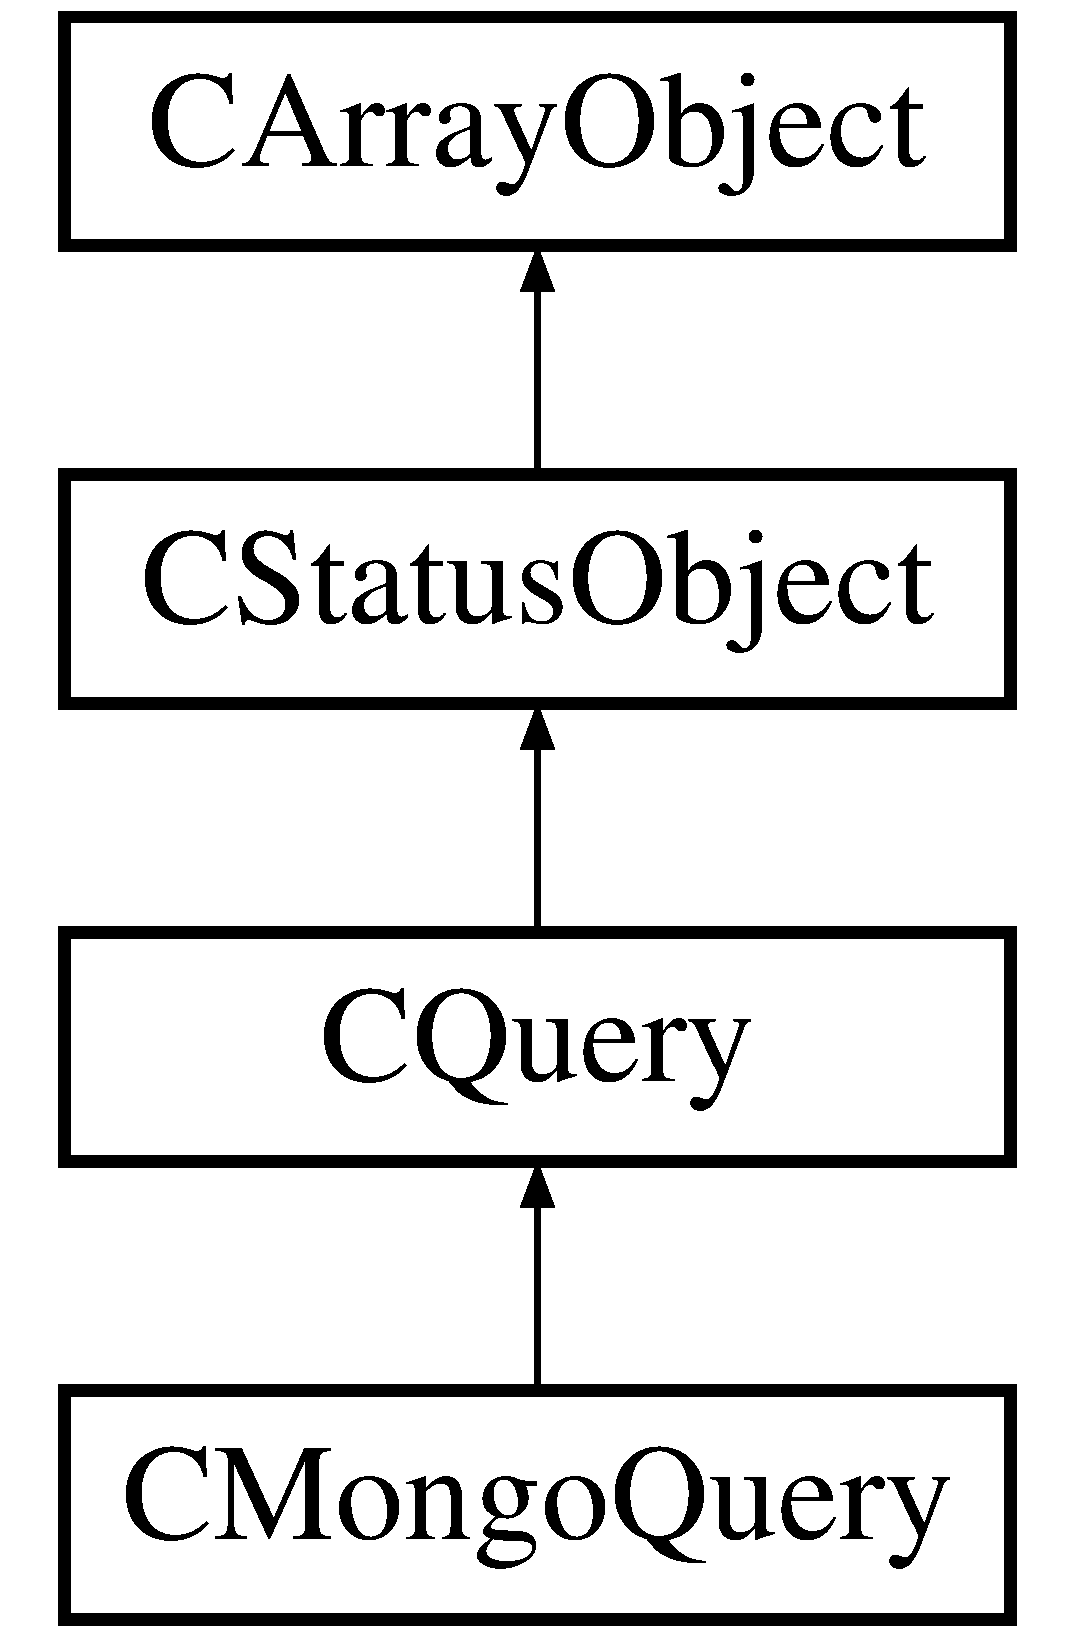
\includegraphics[height=4.000000cm]{class_c_query}
\end{center}
\end{figure}
\subsection*{Public Member Functions}
\begin{DoxyCompactItemize}
\item 
\hyperlink{class_c_query_a5f622c663cffb67955a528cac46502f9}{\-\_\-\-\_\-construct} (\$the\-Query=N\-U\-L\-L)
\item 
\hyperlink{class_c_query_a6cd7ba8e153fc299ba87b614ccb56486}{Append\-Statement} (\$the\-Statement, \$the\-Condition=k\-O\-P\-E\-R\-A\-T\-O\-R\-\_\-\-A\-N\-D)
\item 
\hyperlink{class_c_query_a715ac553707078841213f7b874cbc48e}{Validate} ()
\end{DoxyCompactItemize}
\subsection*{Protected Member Functions}
\begin{DoxyCompactItemize}
\item 
\hyperlink{class_c_query_a1a01d39eedd2951f704dc75c58fb477c}{\-\_\-\-Append\-Statement} (\&\$the\-Query, \$the\-Condition, \$the\-Statement)
\item 
\hyperlink{class_c_query_a5fbde46df4bb30cb252647f0e47cbbde}{\-\_\-\-Validate\-Condition} (\$the\-Condition, \$the\-Statements, \$the\-Level)
\item 
\hyperlink{class_c_query_afe96707c9ed84ee197dae56c9f05f2a4}{\-\_\-\-Validate\-Statement} (\$the\-Statement, \$the\-Level)
\end{DoxyCompactItemize}
\subsection*{Additional Inherited Members}


\subsection{Constructor \& Destructor Documentation}
\hypertarget{class_c_query_a5f622c663cffb67955a528cac46502f9}{\index{C\-Query@{C\-Query}!\-\_\-\-\_\-construct@{\-\_\-\-\_\-construct}}
\index{\-\_\-\-\_\-construct@{\-\_\-\-\_\-construct}!CQuery@{C\-Query}}
\subsubsection[{\-\_\-\-\_\-construct}]{\setlength{\rightskip}{0pt plus 5cm}C\-Query\-::\-\_\-\-\_\-construct (
\begin{DoxyParamCaption}
\item[{}]{\$the\-Query = {\ttfamily NULL}}
\end{DoxyParamCaption}
)}}\label{class_c_query_a5f622c663cffb67955a528cac46502f9}
Instantiate class.

If you omit the parameter the method will instantiate an empty query, if you provide an array or Array\-Object it will assume the structure to be a query and will instantiate the object with it; any other data type will raise an exception.


\begin{DoxyParams}[1]{Parameters}
mixed & {\em \$the\-Query} & Query data.\\
\hline
\end{DoxyParams}
public 

\subsection{Member Function Documentation}
\hypertarget{class_c_query_a1a01d39eedd2951f704dc75c58fb477c}{\index{C\-Query@{C\-Query}!\-\_\-\-Append\-Statement@{\-\_\-\-Append\-Statement}}
\index{\-\_\-\-Append\-Statement@{\-\_\-\-Append\-Statement}!CQuery@{C\-Query}}
\subsubsection[{\-\_\-\-Append\-Statement}]{\setlength{\rightskip}{0pt plus 5cm}C\-Query\-::\-\_\-\-Append\-Statement (
\begin{DoxyParamCaption}
\item[{\&}]{\$the\-Query, }
\item[{}]{\$the\-Condition, }
\item[{}]{\$the\-Statement}
\end{DoxyParamCaption}
)\hspace{0.3cm}{\ttfamily [protected]}}}\label{class_c_query_a1a01d39eedd2951f704dc75c58fb477c}
Append statement.

This method will append the provided statement to the current query.

Statements of the same type, \hyperlink{}{A\-N\-D} and \hyperlink{}{N\-A\-N\-D}, or \hyperlink{}{O\-R} and \hyperlink{}{N\-O\-R}, will be added at the same level. If the top level is an \hyperlink{}{O\-R} or \hyperlink{}{N\-O\-R} and the provided statement is an \hyperlink{}{A\-N\-D} or \hyperlink{}{N\-A\-N\-D}, the latter will be promoted to the top level.

The parameters to this method are\-:


\begin{DoxyItemize}
\item {\bfseries \&\$the\-Query}\-: Query receiving statement. 
\item {\bfseries \$the\-Condition}\-: Statement condition. 
\item {\bfseries \$the\-Condition}\-: Boolean statement condition code. 
\end{DoxyItemize}


\begin{DoxyParams}[1]{Parameters}
reference & {\em \&\$the\-Query} & Query. \\
\hline
array & {\em \$the\-Condition} & Statement condition. \\
\hline
string & {\em \$the\-Statement} & Statement.\\
\hline
\end{DoxyParams}
protected \hypertarget{class_c_query_a5fbde46df4bb30cb252647f0e47cbbde}{\index{C\-Query@{C\-Query}!\-\_\-\-Validate\-Condition@{\-\_\-\-Validate\-Condition}}
\index{\-\_\-\-Validate\-Condition@{\-\_\-\-Validate\-Condition}!CQuery@{C\-Query}}
\subsubsection[{\-\_\-\-Validate\-Condition}]{\setlength{\rightskip}{0pt plus 5cm}C\-Query\-::\-\_\-\-Validate\-Condition (
\begin{DoxyParamCaption}
\item[{}]{\$the\-Condition, }
\item[{}]{\$the\-Statements, }
\item[{}]{\$the\-Level}
\end{DoxyParamCaption}
)\hspace{0.3cm}{\ttfamily [protected]}}}\label{class_c_query_a5fbde46df4bb30cb252647f0e47cbbde}
Validate condition.

This method expects a condition as its argument, it will check if it is a valid condition, then it will \hyperlink{class_c_query_afe96707c9ed84ee197dae56c9f05f2a4}{validate} all condition statements.


\begin{DoxyParams}[1]{Parameters}
string & {\em \$the\-Condition} & Boolean condition. \\
\hline
array & {\em \$the\-Statements} & Statements list. \\
\hline
integer & {\em \$the\-Level} & \mbox{[}P\-R\-I\-V\-A\-T\-E\mbox{]} condition level.\\
\hline
\end{DoxyParams}
protected 

Reimplemented in \hyperlink{class_c_mongo_query_a651af70656cb9894ef1885a711a0c141}{C\-Mongo\-Query}.

\hypertarget{class_c_query_afe96707c9ed84ee197dae56c9f05f2a4}{\index{C\-Query@{C\-Query}!\-\_\-\-Validate\-Statement@{\-\_\-\-Validate\-Statement}}
\index{\-\_\-\-Validate\-Statement@{\-\_\-\-Validate\-Statement}!CQuery@{C\-Query}}
\subsubsection[{\-\_\-\-Validate\-Statement}]{\setlength{\rightskip}{0pt plus 5cm}C\-Query\-::\-\_\-\-Validate\-Statement (
\begin{DoxyParamCaption}
\item[{}]{\$the\-Statement, }
\item[{}]{\$the\-Level}
\end{DoxyParamCaption}
)\hspace{0.3cm}{\ttfamily [protected]}}}\label{class_c_query_afe96707c9ed84ee197dae56c9f05f2a4}
Validate statement.

This method expects a statement as its argument, it will check if it is a valid statement and check if all required elements are there.


\begin{DoxyParams}[1]{Parameters}
array & {\em \$the\-Statement} & Statement. \\
\hline
integer & {\em \$the\-Level} & \mbox{[}P\-R\-I\-V\-A\-T\-E\mbox{]} condition level.\\
\hline
\end{DoxyParams}
protected \hypertarget{class_c_query_a6cd7ba8e153fc299ba87b614ccb56486}{\index{C\-Query@{C\-Query}!Append\-Statement@{Append\-Statement}}
\index{Append\-Statement@{Append\-Statement}!CQuery@{C\-Query}}
\subsubsection[{Append\-Statement}]{\setlength{\rightskip}{0pt plus 5cm}C\-Query\-::\-Append\-Statement (
\begin{DoxyParamCaption}
\item[{}]{\$the\-Statement, }
\item[{}]{\$the\-Condition = {\ttfamily kOPERATOR\-\_\-AND}}
\end{DoxyParamCaption}
)}}\label{class_c_query_a6cd7ba8e153fc299ba87b614ccb56486}
Append statement.

This method will append the provided statement to the query, the second parameter represents the condition.

Appended statements are merged at the condition level\-: if the condition exists at any level, the statement is appended to that condition; if the condition does not exist, it is created. Obviously, \hyperlink{}{A\-N\-D} and \hyperlink{}{N\-A\-N\-D} are treated as equivalent, as well as \hyperlink{}{O\-R} and \hyperlink{}{N\-O\-R}.

If you provide an object derived from \hyperlink{class_c_query}{C\-Query} as the statement, the method will ignore the condition parameter and append the provided query to the current object.


\begin{DoxyParams}[1]{Parameters}
array & {\em \$the\-Statement} & Statement. \\
\hline
string & {\em \$the\-Condition} & Statement condition.\\
\hline
\end{DoxyParams}
public


\begin{DoxyExceptions}{Exceptions}
{\em Exception} & \\
\hline
\end{DoxyExceptions}
\hypertarget{class_c_query_a715ac553707078841213f7b874cbc48e}{\index{C\-Query@{C\-Query}!Validate@{Validate}}
\index{Validate@{Validate}!CQuery@{C\-Query}}
\subsubsection[{Validate}]{\setlength{\rightskip}{0pt plus 5cm}C\-Query\-::\-Validate (
\begin{DoxyParamCaption}
{}
\end{DoxyParamCaption}
)}}\label{class_c_query_a715ac553707078841213f7b874cbc48e}
Validate query.

This method will check whether the query structure is valid.

public


\begin{DoxyExceptions}{Exceptions}
{\em Exception} & \\
\hline
\end{DoxyExceptions}


The documentation for this class was generated from the following file\-:\begin{DoxyCompactItemize}
\item 
/\-Library/\-Web\-Server/\-Library/wrapper/classes/C\-Query.\-php\end{DoxyCompactItemize}

\hypertarget{class_c_query_statement}{\section{C\-Query\-Statement Class Reference}
\label{class_c_query_statement}\index{C\-Query\-Statement@{C\-Query\-Statement}}
}
Inheritance diagram for C\-Query\-Statement\-:\begin{figure}[H]
\begin{center}
\leavevmode
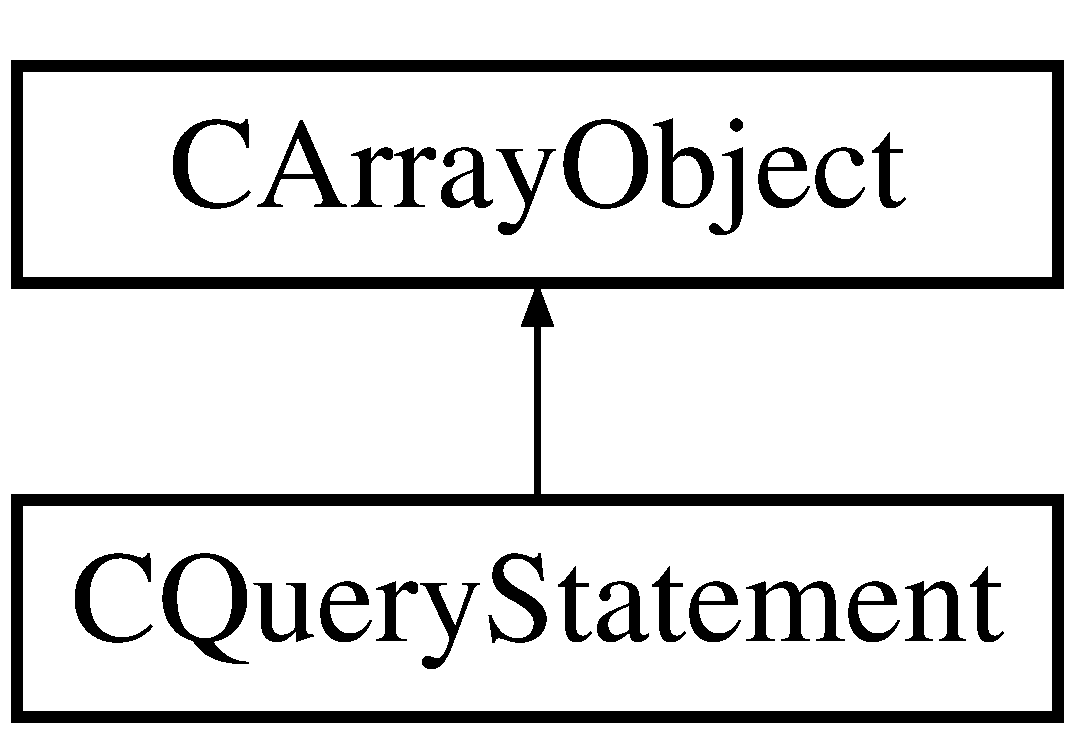
\includegraphics[height=2.000000cm]{class_c_query_statement}
\end{center}
\end{figure}
\subsection*{Public Member Functions}
\begin{DoxyCompactItemize}
\item 
\hyperlink{class_c_query_statement_a996b7a9ae1d54bc3f73de41501b5e02b}{\-\_\-\-\_\-construct} (\$the\-Subject=N\-U\-L\-L, \$the\-Predicate=N\-U\-L\-L, \$the\-Type=N\-U\-L\-L, \$the\-Object=N\-U\-L\-L, \$the\-Range=N\-U\-L\-L)
\item 
\hyperlink{class_c_query_statement_a5a27c44c892286e2fc77dc961d2e30d4}{Subject} (\$the\-Value=N\-U\-L\-L, \$get\-Old=F\-A\-L\-S\-E)
\item 
\hyperlink{class_c_query_statement_ae941698661c8f4b94ce08ea1eaad94b7}{Object} (\$the\-Value=N\-U\-L\-L, \$get\-Old=F\-A\-L\-S\-E)
\item 
\hyperlink{class_c_query_statement_a4a6c6eca496b006e21bfd9c18a31f116}{Predicate} (\$the\-Value=N\-U\-L\-L, \$get\-Old=F\-A\-L\-S\-E)
\item 
\hyperlink{class_c_query_statement_a37bbaad291c18c92954cc25dd49c117b}{Type} (\$the\-Value=N\-U\-L\-L, \$get\-Old=F\-A\-L\-S\-E)
\item 
\hyperlink{class_c_query_statement_a17cf641a4180129015bc0da8e83a7a4c}{Range} (\$the\-Bound1, \$the\-Bound2, \$get\-Old=F\-A\-L\-S\-E)
\end{DoxyCompactItemize}
\subsection*{Static Public Member Functions}
\begin{DoxyCompactItemize}
\item 
static \hyperlink{class_c_query_statement_ac14041ddd7df1cca53aa6594aac7872f}{Disabled} (\$the\-Subject, \$the\-Object=N\-U\-L\-L, \$the\-Type=N\-U\-L\-L, \$the\-Range=N\-U\-L\-L)
\item 
static \hyperlink{class_c_query_statement_a37f7b088b60623ba9435fc400276a828}{Equals} (\$the\-Subject, \$the\-Object, \$the\-Type=N\-U\-L\-L)
\item 
static \hyperlink{class_c_query_statement_a3152dfb1a2eda4047a11ffcd2af50846}{Not\-Equals} (\$the\-Subject, \$the\-Object, \$the\-Type=N\-U\-L\-L)
\item 
static \hyperlink{class_c_query_statement_a26fd9aefa3c9df4228f9aaa7b5d74cbc}{Like} (\$the\-Subject, \$the\-Object)
\item 
static \hyperlink{class_c_query_statement_a6c89cfdf83f46e2fd3ca807254236ed7}{Not\-Like} (\$the\-Subject, \$the\-Object)
\item 
static \hyperlink{class_c_query_statement_a343902e7ebf9facbff20bcd9be63794c}{Prefix} (\$the\-Subject, \$the\-Object)
\item 
static \hyperlink{class_c_query_statement_abdc4fa447abbde5aa34959f6b830a7e0}{Contains} (\$the\-Subject, \$the\-Object)
\item 
static \hyperlink{class_c_query_statement_a80232c348a9db646d3a94bd44611918e}{Suffix} (\$the\-Subject, \$the\-Object)
\item 
static \hyperlink{class_c_query_statement_a952e2d252c4a2a469c03a9e96f151d35}{Regex} (\$the\-Subject, \$the\-Object)
\item 
static \hyperlink{class_c_query_statement_af3a8b31af7f32562fb1ce7ba16f69766}{Less} (\$the\-Subject, \$the\-Object, \$the\-Type=N\-U\-L\-L)
\item 
static \hyperlink{class_c_query_statement_a292880d593cc8b46dba77d13004aaa28}{Less\-Equal} (\$the\-Subject, \$the\-Object, \$the\-Type=N\-U\-L\-L)
\item 
static \hyperlink{class_c_query_statement_abe09c835887534aeecbeffad2045c917}{Great} (\$the\-Subject, \$the\-Object, \$the\-Type=N\-U\-L\-L)
\item 
static \hyperlink{class_c_query_statement_a540d93d646384d5a145d3944d72246e3}{Great\-Equal} (\$the\-Subject, \$the\-Object, \$the\-Type=N\-U\-L\-L)
\item 
static \hyperlink{class_c_query_statement_ae18f91d3c6c1ad07bb380d959ce01c1b}{Range\-Inclusive} (\$the\-Subject, \$the\-Bound1, \$the\-Bound2, \$the\-Type=N\-U\-L\-L)
\item 
static \hyperlink{class_c_query_statement_a182c44c738d574e6d331d5bd894ce8e7}{Range\-Exclusive} (\$the\-Subject, \$the\-Bound1, \$the\-Bound2, \$the\-Type=N\-U\-L\-L)
\item 
static \hyperlink{class_c_query_statement_a45c462050093bf18a5065cb018c91a34}{Missing} (\$the\-Subject)
\item 
static \hyperlink{class_c_query_statement_aba90304323e0de3966810bf1bed26ef4}{Exists} (\$the\-Subject)
\item 
static \hyperlink{class_c_query_statement_a5e1a291d73a20b4f88c019d1863a4c81}{Member} (\$the\-Subject, \$the\-Object, \$the\-Type=N\-U\-L\-L)
\item 
static \hyperlink{class_c_query_statement_aeb90f2ea2237ddc0ab01d9965538abf4}{Not\-Member} (\$the\-Subject, \$the\-Object, \$the\-Type=N\-U\-L\-L)
\item 
static \hyperlink{class_c_query_statement_a7cb662f303eb30652460fd4903053ca8}{All} (\$the\-Subject, \$the\-Object, \$the\-Type=N\-U\-L\-L)
\item 
static \hyperlink{class_c_query_statement_ac3c86273637210e1d117cae10ff9bfe9}{Not\-All} (\$the\-Subject, \$the\-Object, \$the\-Type=N\-U\-L\-L)
\item 
static \hyperlink{class_c_query_statement_ae668b0a35863ac739a188cecd84027a5}{Expression} (\$the\-Subject, \$the\-Object)
\end{DoxyCompactItemize}


\subsection{Constructor \& Destructor Documentation}
\hypertarget{class_c_query_statement_a996b7a9ae1d54bc3f73de41501b5e02b}{\index{C\-Query\-Statement@{C\-Query\-Statement}!\-\_\-\-\_\-construct@{\-\_\-\-\_\-construct}}
\index{\-\_\-\-\_\-construct@{\-\_\-\-\_\-construct}!CQueryStatement@{C\-Query\-Statement}}
\subsubsection[{\-\_\-\-\_\-construct}]{\setlength{\rightskip}{0pt plus 5cm}C\-Query\-Statement\-::\-\_\-\-\_\-construct (
\begin{DoxyParamCaption}
\item[{}]{\$the\-Subject = {\ttfamily NULL}, }
\item[{}]{\$the\-Predicate = {\ttfamily NULL}, }
\item[{}]{\$the\-Type = {\ttfamily NULL}, }
\item[{}]{\$the\-Object = {\ttfamily NULL}, }
\item[{}]{\$the\-Range = {\ttfamily NULL}}
\end{DoxyParamCaption}
)}}\label{class_c_query_statement_a996b7a9ae1d54bc3f73de41501b5e02b}
Instantiate class.

The constructor can be used to instantiate a statement either by providing an existing statement structure, or by providing the statement elements\-:


\begin{DoxyItemize}
\item {\bfseries \$the\-Subject}\-: The statement subject\-: 
\begin{DoxyItemize}
\item {\itshape array} or {\itshape Array\-Object}\-: Structures are interpreted as built statements, so the method will scan the structure and load the corresponding elements. 
\item {\itshape string}\-: Any other type will be converted to a string and interpreted as the statement subject, or data element key. 
\end{DoxyItemize}
\item {\bfseries \$the\-Predicate}\-: The statement operator or predicate\-: 
\begin{DoxyItemize}
\item {\itshape \hyperlink{}{k\-O\-P\-E\-R\-A\-T\-O\-R\-\_\-\-D\-I\-S\-A\-B\-L\-E\-D}}\-: Disabled, it means that the current statement is disabled; the remaining parameters are ignored. 
\item {\itshape \hyperlink{}{k\-O\-P\-E\-R\-A\-T\-O\-R\-\_\-\-E\-Q\-U\-A\-L}}\-: Equality (=), this operator implies that the method expects the next two parameters. 
\item {\itshape \hyperlink{}{k\-O\-P\-E\-R\-A\-T\-O\-R\-\_\-\-E\-Q\-U\-A\-L\-\_\-\-N\-O\-T}}\-: Inequality (!=), negates the \hyperlink{}{k\-O\-P\-E\-R\-A\-T\-O\-R\-\_\-\-E\-Q\-U\-A\-L} operator; this operator implies that the method expects the next two parameters. 
\item {\itshape \hyperlink{}{k\-O\-P\-E\-R\-A\-T\-O\-R\-\_\-\-L\-I\-K\-E}}\-: Like, it is an accent and case insensitive equality filter, this operator implies that the method expects the next two parameters. 
\item {\itshape \hyperlink{}{k\-O\-P\-E\-R\-A\-T\-O\-R\-\_\-\-L\-I\-K\-E\-\_\-\-N\-O\-T}}\-: The negation of the \hyperlink{}{L\-I\-K\-E} operator, this operator implies that the method expects the next two parameters. 
\item {\itshape \hyperlink{}{k\-O\-P\-E\-R\-A\-T\-O\-R\-\_\-\-P\-R\-E\-F\-I\-X}}\-: Starts with, or prefix match, this operator implies that the method expects the next two parameters. 
\item {\itshape \hyperlink{}{k\-O\-P\-E\-R\-A\-T\-O\-R\-\_\-\-C\-O\-N\-T\-A\-I\-N\-S}}\-: Contains, selects all elements that contain the match string, this operator implies that the method expects the next two parameters. 
\item {\itshape \hyperlink{}{k\-O\-P\-E\-R\-A\-T\-O\-R\-\_\-\-S\-U\-F\-F\-I\-X}}\-: Ends with, or suffix match, this operator implies that the method expects the next two parameters. 
\item {\itshape \hyperlink{}{k\-O\-P\-E\-R\-A\-T\-O\-R\-\_\-\-R\-E\-G\-E\-X}}\-: Regular expression, this operator implies that the method expects the next two parameters. 
\item {\itshape \hyperlink{}{k\-O\-P\-E\-R\-A\-T\-O\-R\-\_\-\-L\-E\-S\-S}}\-: Smaller than ($<$), this operator implies that the method expects the next two parameters. 
\item {\itshape \hyperlink{}{k\-O\-P\-E\-R\-A\-T\-O\-R\-\_\-\-L\-E\-S\-S\-\_\-\-E\-Q\-U\-A\-L}}\-: Smaller than or equal ($<$=), this operator implies that the method expects the next two parameters. 
\item {\itshape \hyperlink{}{k\-O\-P\-E\-R\-A\-T\-O\-R\-\_\-\-G\-R\-E\-A\-T}}\-: Greater than ($>$), this operator implies that the method expects the next two parameters. 
\item {\itshape \hyperlink{}{k\-O\-P\-E\-R\-A\-T\-O\-R\-\_\-\-G\-R\-E\-A\-T\-\_\-\-E\-Q\-U\-A\-L}}\-: Greater than or equal ($>$=), this operator implies that the method expects the next two parameters. 
\item {\itshape \hyperlink{}{k\-O\-P\-E\-R\-A\-T\-O\-R\-\_\-\-I\-R\-A\-N\-G\-E}}\-: Range inclusive, matches $>$= value $<$=; this operator implies that the method expects the next three parameters. 
\item {\itshape \hyperlink{}{k\-O\-P\-E\-R\-A\-T\-O\-R\-\_\-\-E\-R\-A\-N\-G\-E}}\-: Range exclusive, matches $>$ value $<$, this operator implies that the method expects the next three parameters. 
\item {\itshape \hyperlink{}{k\-O\-P\-E\-R\-A\-T\-O\-R\-\_\-\-N\-U\-L\-L}}\-: Is {\itshape N\-U\-L\-L} or element is missing. 
\item {\itshape \hyperlink{}{k\-O\-P\-E\-R\-A\-T\-O\-R\-\_\-\-N\-O\-T\-\_\-\-N\-U\-L\-L}}\-:Not {\itshape N\-U\-L\-L} or element exists. 
\item {\itshape \hyperlink{}{k\-O\-P\-E\-R\-A\-T\-O\-R\-\_\-\-I\-N}}\-: In, or belongs to set, this operator implies that the method expects the next two parameters. 
\item {\itshape \hyperlink{}{k\-O\-P\-E\-R\-A\-T\-O\-R\-\_\-\-N\-I}}\-: Not in, the negation of \hyperlink{}{k\-O\-P\-E\-R\-A\-T\-O\-R\-\_\-\-I\-N}, this operator implies that the method expects the next two parameters. 
\item {\itshape \hyperlink{}{k\-O\-P\-E\-R\-A\-T\-O\-R\-\_\-\-A\-L\-L}}\-: All, or match the full set, this operator implies that the method expects the next two parameters. 
\item {\itshape \hyperlink{}{k\-O\-P\-E\-R\-A\-T\-O\-R\-\_\-\-N\-A\-L\-L}}\-: Not all, the negation of the \hyperlink{}{k\-O\-P\-E\-R\-A\-T\-O\-R\-\_\-\-A\-L\-L} operator, this operator implies that the method expects the next two parameters. 
\item {\itshape \hyperlink{}{k\-O\-P\-E\-R\-A\-T\-O\-R\-\_\-\-E\-X}}\-: Expression, indicates a complex expression, this operator implies that the method expects the next two parameters. 
\end{DoxyItemize}
\item {\bfseries \$the\-Type}\-: The statement object data type, this qualifies all remaining parameters. The allowed values are\-: 
\begin{DoxyItemize}
\item {\itshape \hyperlink{}{k\-T\-Y\-P\-E\-\_\-\-S\-T\-R\-I\-N\-G}}\-: String, we assume in U\-T\-F8 character set, the string is expected in the next parameter. 
\item {\itshape \hyperlink{}{k\-T\-Y\-P\-E\-\_\-\-I\-N\-T32}}\-: 32 bit signed integer, the number is expected in the next parameter, either as an integer, float or string; once received, it will be converted to a \hyperlink{class_c_data_type_int32}{C\-Data\-Type\-Int32} object. 
\item {\itshape \hyperlink{}{k\-T\-Y\-P\-E\-\_\-\-I\-N\-T64}}\-: 64 bit signed integer, the number is expected in the next parameter, either as an integer, float or string; once received, it will be converted to a \hyperlink{class_c_data_type_int64}{C\-Data\-Type\-Int64} object. 
\item {\itshape \hyperlink{}{k\-T\-Y\-P\-E\-\_\-\-F\-L\-O\-A\-T}}\-: Floating point number, the number is expected in the next parameter, either as an integer, float or string. 
\item {\itshape \hyperlink{}{k\-T\-Y\-P\-E\-\_\-\-D\-A\-T\-E}}\-: A string date, it is treated as a string date with a Y\-Y\-Y\-Y\-M\-M\-D\-D format in which month and day may be omitted. 
\item {\itshape \hyperlink{}{k\-T\-Y\-P\-E\-\_\-\-T\-I\-M\-E}}\-: A string time, it is treated as a string time with a Y\-Y\-Y\-Y-\/\-M\-M-\/\-D\-D H\-H\-:\-M\-M\-:S\-S format in which all elements are required; this element will be converted to a \hyperlink{}{k\-T\-Y\-P\-E\-\_\-\-S\-T\-A\-M\-P} data type. 
\item {\itshape \hyperlink{}{k\-T\-Y\-P\-E\-\_\-\-S\-T\-A\-M\-P}}\-: A timestamp, optionally including microseconds, elements of this type will be converted to \hyperlink{class_c_data_type_stamp}{C\-Data\-Type\-Stamp} objects. 
\item {\itshape \hyperlink{}{k\-T\-Y\-P\-E\-\_\-\-B\-O\-O\-L\-E\-A\-N}}\-: An on/off switch, it will be converted to a 1/0 pair. 
\item {\itshape \hyperlink{}{k\-T\-Y\-P\-E\-\_\-\-B\-I\-N\-A\-R\-Y}}\-: A binary string, the string will be converted to a \hyperlink{class_c_data_type_binary}{C\-Data\-Type\-Binary} object. 
\end{DoxyItemize}
\item {\bfseries \$the\-Object}\-: The statement object data, it should reflect the data type provided in the previous parameter. 
\item {\bfseries \$the\-Range}\-: The statement range end or second element. This value must also reflect the data type provided in the previous parameter and will be automatically set if you provided a range and forgot to set it. 
\end{DoxyItemize}


\begin{DoxyParams}[1]{Parameters}
mixed & {\em \$the\-Subject} & Statement subject. \\
\hline
string & {\em \$the\-Predicate} & Statement predicate. \\
\hline
string & {\em \$the\-Type} & Statement object data type. \\
\hline
mixed & {\em \$the\-Object} & Statement object or first range. \\
\hline
mixed & {\em \$the\-Range} & Statement second range.\\
\hline
\end{DoxyParams}
public 

\subsection{Member Function Documentation}
\hypertarget{class_c_query_statement_a7cb662f303eb30652460fd4903053ca8}{\index{C\-Query\-Statement@{C\-Query\-Statement}!All@{All}}
\index{All@{All}!CQueryStatement@{C\-Query\-Statement}}
\subsubsection[{All}]{\setlength{\rightskip}{0pt plus 5cm}static C\-Query\-Statement\-::\-All (
\begin{DoxyParamCaption}
\item[{}]{\$the\-Subject, }
\item[{}]{\$the\-Object, }
\item[{}]{\$the\-Type = {\ttfamily NULL}}
\end{DoxyParamCaption}
)\hspace{0.3cm}{\ttfamily [static]}}}\label{class_c_query_statement_a7cb662f303eb30652460fd4903053ca8}
Create an \hyperlink{}{all} statement.

This method can be used to instantiate an \hyperlink{}{all} query statement which will test whether all the \hyperlink{class_c_query_statement_a5a27c44c892286e2fc77dc961d2e30d4}{subject} values can be found in the provided \hyperlink{class_c_query_statement_ae941698661c8f4b94ce08ea1eaad94b7}{object}, which will be interpreted as a list of values.

If the provided \hyperlink{class_c_query_statement_ae941698661c8f4b94ce08ea1eaad94b7}{object} is not an array or an Array\-Object, the method will add it to a newly created array.

The statement uses the \hyperlink{}{k\-O\-P\-E\-R\-A\-T\-O\-R\-\_\-\-A\-L\-L} operator and this method accepts the following parameters\-:


\begin{DoxyItemize}
\item {\bfseries \$the\-Subject}\-: Statement \hyperlink{class_c_query_statement_a5a27c44c892286e2fc77dc961d2e30d4}{subject}. 
\item {\bfseries \$the\-Object}\-: Statement \hyperlink{class_c_query_statement_ae941698661c8f4b94ce08ea1eaad94b7}{object}, or members list. 
\item {\bfseries \$the\-Type}\-: Statement object data \hyperlink{class_c_query_statement_a37bbaad291c18c92954cc25dd49c117b}{type}. 
\end{DoxyItemize}

The method will return an instance of this class or raise an exception on errors.


\begin{DoxyParams}[1]{Parameters}
mixed & {\em \$the\-Subject} & Statement subject. \\
\hline
mixed & {\em \$the\-Object} & Statement object. \\
\hline
string & {\em \$the\-Type} & Statement object data type.\\
\hline
\end{DoxyParams}
\begin{DoxySeeAlso}{See also}
k\-O\-P\-E\-R\-A\-T\-O\-R\-\_\-\-A\-L\-L 
\end{DoxySeeAlso}
\hypertarget{class_c_query_statement_abdc4fa447abbde5aa34959f6b830a7e0}{\index{C\-Query\-Statement@{C\-Query\-Statement}!Contains@{Contains}}
\index{Contains@{Contains}!CQueryStatement@{C\-Query\-Statement}}
\subsubsection[{Contains}]{\setlength{\rightskip}{0pt plus 5cm}static C\-Query\-Statement\-::\-Contains (
\begin{DoxyParamCaption}
\item[{}]{\$the\-Subject, }
\item[{}]{\$the\-Object}
\end{DoxyParamCaption}
)\hspace{0.3cm}{\ttfamily [static]}}}\label{class_c_query_statement_abdc4fa447abbde5aa34959f6b830a7e0}
Create a \hyperlink{}{contains} statement.

This method can be used to instantiate a query statement that will select all elements whose contents matches the test data in any position.

The statement uses the \hyperlink{}{k\-O\-P\-E\-R\-A\-T\-O\-R\-\_\-\-C\-O\-N\-T\-A\-I\-N\-S} operator and this method accepts the following parameters\-:


\begin{DoxyItemize}
\item {\bfseries \$the\-Subject}\-: Statement \hyperlink{class_c_query_statement_a5a27c44c892286e2fc77dc961d2e30d4}{subject}. 
\item {\bfseries \$the\-Object}\-: Statement \hyperlink{class_c_query_statement_ae941698661c8f4b94ce08ea1eaad94b7}{object} match sub-\/string. 
\end{DoxyItemize}

Note that the data type is implicitly a \hyperlink{}{string}

The method will return an instance of this class or raise an exception on errors.


\begin{DoxyParams}[1]{Parameters}
mixed & {\em \$the\-Subject} & Statement subject. \\
\hline
mixed & {\em \$the\-Object} & Statement object.\\
\hline
\end{DoxyParams}
\begin{DoxySeeAlso}{See also}
k\-O\-P\-E\-R\-A\-T\-O\-R\-\_\-\-C\-O\-N\-T\-A\-I\-N\-S k\-T\-Y\-P\-E\-\_\-\-S\-T\-R\-I\-N\-G 
\end{DoxySeeAlso}
\hypertarget{class_c_query_statement_ac14041ddd7df1cca53aa6594aac7872f}{\index{C\-Query\-Statement@{C\-Query\-Statement}!Disabled@{Disabled}}
\index{Disabled@{Disabled}!CQueryStatement@{C\-Query\-Statement}}
\subsubsection[{Disabled}]{\setlength{\rightskip}{0pt plus 5cm}static C\-Query\-Statement\-::\-Disabled (
\begin{DoxyParamCaption}
\item[{}]{\$the\-Subject, }
\item[{}]{\$the\-Object = {\ttfamily NULL}, }
\item[{}]{\$the\-Type = {\ttfamily NULL}, }
\item[{}]{\$the\-Range = {\ttfamily NULL}}
\end{DoxyParamCaption}
)\hspace{0.3cm}{\ttfamily [static]}}}\label{class_c_query_statement_ac14041ddd7df1cca53aa6594aac7872f}
Create a disabled statement.

This method can be used to instantiate a disabled query statement. A disabled statement is one that should not execute, it can be used as a placeholder, or external methods may disable statements.

The statement uses the \hyperlink{}{k\-O\-P\-E\-R\-A\-T\-O\-R\-\_\-\-D\-I\-S\-A\-B\-L\-E\-D} operator and this method accepts the following parameters\-:


\begin{DoxyItemize}
\item {\bfseries \$the\-Subject}\-: Statement \hyperlink{class_c_query_statement_a5a27c44c892286e2fc77dc961d2e30d4}{subject}. 
\item {\bfseries \$the\-Object}\-: Statement \hyperlink{class_c_query_statement_ae941698661c8f4b94ce08ea1eaad94b7}{object} or first \hyperlink{class_c_query_statement_a17cf641a4180129015bc0da8e83a7a4c}{range} bound. 
\item {\bfseries \$the\-Type}\-: Statement object data \hyperlink{class_c_query_statement_a37bbaad291c18c92954cc25dd49c117b}{type}. 
\item {\bfseries \$the\-Range}\-: Statement second \hyperlink{class_c_query_statement_a17cf641a4180129015bc0da8e83a7a4c}{range} bound. 
\end{DoxyItemize}

The method will return an instance of this class or raise an exception on errors.


\begin{DoxyParams}[1]{Parameters}
mixed & {\em \$the\-Subject} & Statement subject. \\
\hline
mixed & {\em \$the\-Object} & Statement object or range bound. \\
\hline
string & {\em \$the\-Type} & Statement object data type. \\
\hline
mixed & {\em \$the\-Range} & Statement range bound.\\
\hline
\end{DoxyParams}
\begin{DoxySeeAlso}{See also}
k\-O\-P\-E\-R\-A\-T\-O\-R\-\_\-\-D\-I\-S\-A\-B\-L\-E\-D 
\end{DoxySeeAlso}
\hypertarget{class_c_query_statement_a37f7b088b60623ba9435fc400276a828}{\index{C\-Query\-Statement@{C\-Query\-Statement}!Equals@{Equals}}
\index{Equals@{Equals}!CQueryStatement@{C\-Query\-Statement}}
\subsubsection[{Equals}]{\setlength{\rightskip}{0pt plus 5cm}static C\-Query\-Statement\-::\-Equals (
\begin{DoxyParamCaption}
\item[{}]{\$the\-Subject, }
\item[{}]{\$the\-Object, }
\item[{}]{\$the\-Type = {\ttfamily NULL}}
\end{DoxyParamCaption}
)\hspace{0.3cm}{\ttfamily [static]}}}\label{class_c_query_statement_a37f7b088b60623ba9435fc400276a828}
Create an \hyperlink{}{equals} statement.

This method can be used to instantiate an \hyperlink{}{equality} query statement.

The statement uses the \hyperlink{}{k\-O\-P\-E\-R\-A\-T\-O\-R\-\_\-\-E\-Q\-U\-A\-L} operator and this method accepts the following parameters\-:


\begin{DoxyItemize}
\item {\bfseries \$the\-Subject}\-: Statement \hyperlink{class_c_query_statement_a5a27c44c892286e2fc77dc961d2e30d4}{subject}. 
\item {\bfseries \$the\-Object}\-: Statement \hyperlink{class_c_query_statement_ae941698661c8f4b94ce08ea1eaad94b7}{object}. 
\item {\bfseries \$the\-Type}\-: Statement object data \hyperlink{class_c_query_statement_a37bbaad291c18c92954cc25dd49c117b}{type}. 
\end{DoxyItemize}

The method will return an instance of this class or raise an exception on errors.


\begin{DoxyParams}[1]{Parameters}
mixed & {\em \$the\-Subject} & Statement subject. \\
\hline
mixed & {\em \$the\-Object} & Statement object. \\
\hline
string & {\em \$the\-Type} & Statement object data type.\\
\hline
\end{DoxyParams}
\begin{DoxySeeAlso}{See also}
k\-O\-P\-E\-R\-A\-T\-O\-R\-\_\-\-E\-Q\-U\-A\-L 
\end{DoxySeeAlso}
\hypertarget{class_c_query_statement_aba90304323e0de3966810bf1bed26ef4}{\index{C\-Query\-Statement@{C\-Query\-Statement}!Exists@{Exists}}
\index{Exists@{Exists}!CQueryStatement@{C\-Query\-Statement}}
\subsubsection[{Exists}]{\setlength{\rightskip}{0pt plus 5cm}static C\-Query\-Statement\-::\-Exists (
\begin{DoxyParamCaption}
\item[{}]{\$the\-Subject}
\end{DoxyParamCaption}
)\hspace{0.3cm}{\ttfamily [static]}}}\label{class_c_query_statement_aba90304323e0de3966810bf1bed26ef4}
Create an \hyperlink{}{exists} statement.

This method can be used to instantiate a \hyperlink{}{missing} or null query statement, the statement will check if the \hyperlink{class_c_query_statement_a5a27c44c892286e2fc77dc961d2e30d4}{subject} exists or is not {\itshape N\-U\-L\-L}.

The statement uses the \hyperlink{}{k\-O\-P\-E\-R\-A\-T\-O\-R\-\_\-\-N\-O\-T\-\_\-\-N\-U\-L\-L} operator and this method accepts the following parameters\-:


\begin{DoxyItemize}
\item {\bfseries \$the\-Subject}\-: Statement \hyperlink{class_c_query_statement_a5a27c44c892286e2fc77dc961d2e30d4}{subject}. 
\end{DoxyItemize}

The method will return an instance of this class or raise an exception on errors.


\begin{DoxyParams}[1]{Parameters}
mixed & {\em \$the\-Subject} & Statement subject.\\
\hline
\end{DoxyParams}
\begin{DoxySeeAlso}{See also}
k\-O\-P\-E\-R\-A\-T\-O\-R\-\_\-\-N\-O\-T\-\_\-\-N\-U\-L\-L 
\end{DoxySeeAlso}
\hypertarget{class_c_query_statement_ae668b0a35863ac739a188cecd84027a5}{\index{C\-Query\-Statement@{C\-Query\-Statement}!Expression@{Expression}}
\index{Expression@{Expression}!CQueryStatement@{C\-Query\-Statement}}
\subsubsection[{Expression}]{\setlength{\rightskip}{0pt plus 5cm}static C\-Query\-Statement\-::\-Expression (
\begin{DoxyParamCaption}
\item[{}]{\$the\-Subject, }
\item[{}]{\$the\-Object}
\end{DoxyParamCaption}
)\hspace{0.3cm}{\ttfamily [static]}}}\label{class_c_query_statement_ae668b0a35863ac739a188cecd84027a5}
Create an \hyperlink{}{expression} statement.

This method can be used to instantiate an \hyperlink{}{expression} query statement in which the object of the statement represents an expression.

Note that in this case the \hyperlink{class_c_query_statement_a37bbaad291c18c92954cc25dd49c117b}{type} is not relevant and it is set by default as a \hyperlink{}{string}.

The statement uses the \hyperlink{}{k\-O\-P\-E\-R\-A\-T\-O\-R\-\_\-\-E\-X} operator and this method accepts the following parameters\-:


\begin{DoxyItemize}
\item {\bfseries \$the\-Subject}\-: Statement \hyperlink{class_c_query_statement_a5a27c44c892286e2fc77dc961d2e30d4}{subject}. 
\item {\bfseries \$the\-Object}\-: Statement \hyperlink{class_c_query_statement_ae941698661c8f4b94ce08ea1eaad94b7}{object}, or comparaison value. 
\item {\bfseries \$the\-Type}\-: Statement object data \hyperlink{class_c_query_statement_a37bbaad291c18c92954cc25dd49c117b}{type}. 
\end{DoxyItemize}

The method will return an instance of this class or raise an exception on errors.


\begin{DoxyParams}[1]{Parameters}
mixed & {\em \$the\-Subject} & Statement subject. \\
\hline
mixed & {\em \$the\-Object} & Statement object or expression.\\
\hline
\end{DoxyParams}
\begin{DoxySeeAlso}{See also}
k\-O\-P\-E\-R\-A\-T\-O\-R\-\_\-\-E\-X k\-T\-Y\-P\-E\-\_\-\-S\-T\-R\-I\-N\-G 
\end{DoxySeeAlso}
\hypertarget{class_c_query_statement_abe09c835887534aeecbeffad2045c917}{\index{C\-Query\-Statement@{C\-Query\-Statement}!Great@{Great}}
\index{Great@{Great}!CQueryStatement@{C\-Query\-Statement}}
\subsubsection[{Great}]{\setlength{\rightskip}{0pt plus 5cm}static C\-Query\-Statement\-::\-Great (
\begin{DoxyParamCaption}
\item[{}]{\$the\-Subject, }
\item[{}]{\$the\-Object, }
\item[{}]{\$the\-Type = {\ttfamily NULL}}
\end{DoxyParamCaption}
)\hspace{0.3cm}{\ttfamily [static]}}}\label{class_c_query_statement_abe09c835887534aeecbeffad2045c917}
Create a \hyperlink{}{greater} than statement.

This method can be used to instantiate a \hyperlink{}{greater} than query statement.

The statement uses the \hyperlink{}{k\-O\-P\-E\-R\-A\-T\-O\-R\-\_\-\-G\-R\-E\-A\-T} operator and this method accepts the following parameters\-:


\begin{DoxyItemize}
\item {\bfseries \$the\-Subject}\-: Statement \hyperlink{class_c_query_statement_a5a27c44c892286e2fc77dc961d2e30d4}{subject}. 
\item {\bfseries \$the\-Object}\-: Statement \hyperlink{class_c_query_statement_ae941698661c8f4b94ce08ea1eaad94b7}{object}, or comparaison value. 
\item {\bfseries \$the\-Type}\-: Statement object data \hyperlink{class_c_query_statement_a37bbaad291c18c92954cc25dd49c117b}{type}. 
\end{DoxyItemize}

The method will return an instance of this class or raise an exception on errors.


\begin{DoxyParams}[1]{Parameters}
mixed & {\em \$the\-Subject} & Statement subject. \\
\hline
mixed & {\em \$the\-Object} & Statement object. \\
\hline
string & {\em \$the\-Type} & Statement object data type.\\
\hline
\end{DoxyParams}
\begin{DoxySeeAlso}{See also}
k\-O\-P\-E\-R\-A\-T\-O\-R\-\_\-\-G\-R\-E\-A\-T 
\end{DoxySeeAlso}
\hypertarget{class_c_query_statement_a540d93d646384d5a145d3944d72246e3}{\index{C\-Query\-Statement@{C\-Query\-Statement}!Great\-Equal@{Great\-Equal}}
\index{Great\-Equal@{Great\-Equal}!CQueryStatement@{C\-Query\-Statement}}
\subsubsection[{Great\-Equal}]{\setlength{\rightskip}{0pt plus 5cm}static C\-Query\-Statement\-::\-Great\-Equal (
\begin{DoxyParamCaption}
\item[{}]{\$the\-Subject, }
\item[{}]{\$the\-Object, }
\item[{}]{\$the\-Type = {\ttfamily NULL}}
\end{DoxyParamCaption}
)\hspace{0.3cm}{\ttfamily [static]}}}\label{class_c_query_statement_a540d93d646384d5a145d3944d72246e3}
Create a \hyperlink{}{greater} than or equal statement.

This method can be used to instantiate a \hyperlink{}{greater} than or equal query statement.

The statement uses the \hyperlink{}{k\-O\-P\-E\-R\-A\-T\-O\-R\-\_\-\-G\-R\-E\-A\-T\-\_\-\-E\-Q\-U\-A\-L} operator and this method accepts the following parameters\-:


\begin{DoxyItemize}
\item {\bfseries \$the\-Subject}\-: Statement \hyperlink{class_c_query_statement_a5a27c44c892286e2fc77dc961d2e30d4}{subject}. 
\item {\bfseries \$the\-Object}\-: Statement \hyperlink{class_c_query_statement_ae941698661c8f4b94ce08ea1eaad94b7}{object}, or comparaison value. 
\item {\bfseries \$the\-Type}\-: Statement object data \hyperlink{class_c_query_statement_a37bbaad291c18c92954cc25dd49c117b}{type}. 
\end{DoxyItemize}

The method will return an instance of this class or raise an exception on errors.


\begin{DoxyParams}[1]{Parameters}
mixed & {\em \$the\-Subject} & Statement subject. \\
\hline
mixed & {\em \$the\-Object} & Statement object. \\
\hline
string & {\em \$the\-Type} & Statement object data type.\\
\hline
\end{DoxyParams}
\begin{DoxySeeAlso}{See also}
k\-O\-P\-E\-R\-A\-T\-O\-R\-\_\-\-G\-R\-E\-A\-T\-\_\-\-E\-Q\-U\-A\-L 
\end{DoxySeeAlso}
\hypertarget{class_c_query_statement_af3a8b31af7f32562fb1ce7ba16f69766}{\index{C\-Query\-Statement@{C\-Query\-Statement}!Less@{Less}}
\index{Less@{Less}!CQueryStatement@{C\-Query\-Statement}}
\subsubsection[{Less}]{\setlength{\rightskip}{0pt plus 5cm}static C\-Query\-Statement\-::\-Less (
\begin{DoxyParamCaption}
\item[{}]{\$the\-Subject, }
\item[{}]{\$the\-Object, }
\item[{}]{\$the\-Type = {\ttfamily NULL}}
\end{DoxyParamCaption}
)\hspace{0.3cm}{\ttfamily [static]}}}\label{class_c_query_statement_af3a8b31af7f32562fb1ce7ba16f69766}
Create a \hyperlink{}{less} than statement.

This method can be used to instantiate a \hyperlink{}{less} than query statement.

The statement uses the \hyperlink{}{k\-O\-P\-E\-R\-A\-T\-O\-R\-\_\-\-L\-E\-S\-S} operator and this method accepts the following parameters\-:


\begin{DoxyItemize}
\item {\bfseries \$the\-Subject}\-: Statement \hyperlink{class_c_query_statement_a5a27c44c892286e2fc77dc961d2e30d4}{subject}. 
\item {\bfseries \$the\-Object}\-: Statement \hyperlink{class_c_query_statement_ae941698661c8f4b94ce08ea1eaad94b7}{object}, or comparaison value. 
\item {\bfseries \$the\-Type}\-: Statement object data \hyperlink{class_c_query_statement_a37bbaad291c18c92954cc25dd49c117b}{type}. 
\end{DoxyItemize}

The method will return an instance of this class or raise an exception on errors.


\begin{DoxyParams}[1]{Parameters}
mixed & {\em \$the\-Subject} & Statement subject. \\
\hline
mixed & {\em \$the\-Object} & Statement object. \\
\hline
string & {\em \$the\-Type} & Statement object data type.\\
\hline
\end{DoxyParams}
\begin{DoxySeeAlso}{See also}
k\-O\-P\-E\-R\-A\-T\-O\-R\-\_\-\-L\-E\-S\-S 
\end{DoxySeeAlso}
\hypertarget{class_c_query_statement_a292880d593cc8b46dba77d13004aaa28}{\index{C\-Query\-Statement@{C\-Query\-Statement}!Less\-Equal@{Less\-Equal}}
\index{Less\-Equal@{Less\-Equal}!CQueryStatement@{C\-Query\-Statement}}
\subsubsection[{Less\-Equal}]{\setlength{\rightskip}{0pt plus 5cm}static C\-Query\-Statement\-::\-Less\-Equal (
\begin{DoxyParamCaption}
\item[{}]{\$the\-Subject, }
\item[{}]{\$the\-Object, }
\item[{}]{\$the\-Type = {\ttfamily NULL}}
\end{DoxyParamCaption}
)\hspace{0.3cm}{\ttfamily [static]}}}\label{class_c_query_statement_a292880d593cc8b46dba77d13004aaa28}
Create a \hyperlink{}{less} than or equal statement.

This method can be used to instantiate a \hyperlink{}{less} than or equal query statement.

The statement uses the \hyperlink{}{k\-O\-P\-E\-R\-A\-T\-O\-R\-\_\-\-L\-E\-S\-S\-\_\-\-E\-Q\-U\-A\-L} operator and this method accepts the following parameters\-:


\begin{DoxyItemize}
\item {\bfseries \$the\-Subject}\-: Statement \hyperlink{class_c_query_statement_a5a27c44c892286e2fc77dc961d2e30d4}{subject}. 
\item {\bfseries \$the\-Object}\-: Statement \hyperlink{class_c_query_statement_ae941698661c8f4b94ce08ea1eaad94b7}{object}, or comparaison value. 
\item {\bfseries \$the\-Type}\-: Statement object data \hyperlink{class_c_query_statement_a37bbaad291c18c92954cc25dd49c117b}{type}. 
\end{DoxyItemize}

The method will return an instance of this class or raise an exception on errors.


\begin{DoxyParams}[1]{Parameters}
mixed & {\em \$the\-Subject} & Statement subject. \\
\hline
mixed & {\em \$the\-Object} & Statement object. \\
\hline
string & {\em \$the\-Type} & Statement object data type.\\
\hline
\end{DoxyParams}
\begin{DoxySeeAlso}{See also}
k\-O\-P\-E\-R\-A\-T\-O\-R\-\_\-\-L\-E\-S\-S\-\_\-\-E\-Q\-U\-A\-L 
\end{DoxySeeAlso}
\hypertarget{class_c_query_statement_a26fd9aefa3c9df4228f9aaa7b5d74cbc}{\index{C\-Query\-Statement@{C\-Query\-Statement}!Like@{Like}}
\index{Like@{Like}!CQueryStatement@{C\-Query\-Statement}}
\subsubsection[{Like}]{\setlength{\rightskip}{0pt plus 5cm}static C\-Query\-Statement\-::\-Like (
\begin{DoxyParamCaption}
\item[{}]{\$the\-Subject, }
\item[{}]{\$the\-Object}
\end{DoxyParamCaption}
)\hspace{0.3cm}{\ttfamily [static]}}}\label{class_c_query_statement_a26fd9aefa3c9df4228f9aaa7b5d74cbc}
Create a case and accent \hyperlink{}{insensitive} equality statement.

This method can be used to instantiate a \hyperlink{}{L\-I\-K\-E} query statement, which is equivalent to the S\-Q\-L {\itshape L\-I\-K\-E} clause, an accent and case insensitive comparaison.

The statement uses the \hyperlink{}{k\-O\-P\-E\-R\-A\-T\-O\-R\-\_\-\-L\-I\-K\-E} operator and this method accepts the following parameters\-:


\begin{DoxyItemize}
\item {\bfseries \$the\-Subject}\-: Statement \hyperlink{class_c_query_statement_a5a27c44c892286e2fc77dc961d2e30d4}{subject}. 
\item {\bfseries \$the\-Object}\-: Statement \hyperlink{class_c_query_statement_ae941698661c8f4b94ce08ea1eaad94b7}{object} match string. 
\end{DoxyItemize}

Note that the data type is implicitly a \hyperlink{}{string}

The method will return an instance of this class or raise an exception on errors.


\begin{DoxyParams}[1]{Parameters}
mixed & {\em \$the\-Subject} & Statement subject. \\
\hline
mixed & {\em \$the\-Object} & Statement object.\\
\hline
\end{DoxyParams}
\begin{DoxySeeAlso}{See also}
k\-O\-P\-E\-R\-A\-T\-O\-R\-\_\-\-L\-I\-K\-E k\-T\-Y\-P\-E\-\_\-\-S\-T\-R\-I\-N\-G 
\end{DoxySeeAlso}
\hypertarget{class_c_query_statement_a5e1a291d73a20b4f88c019d1863a4c81}{\index{C\-Query\-Statement@{C\-Query\-Statement}!Member@{Member}}
\index{Member@{Member}!CQueryStatement@{C\-Query\-Statement}}
\subsubsection[{Member}]{\setlength{\rightskip}{0pt plus 5cm}static C\-Query\-Statement\-::\-Member (
\begin{DoxyParamCaption}
\item[{}]{\$the\-Subject, }
\item[{}]{\$the\-Object, }
\item[{}]{\$the\-Type = {\ttfamily NULL}}
\end{DoxyParamCaption}
)\hspace{0.3cm}{\ttfamily [static]}}}\label{class_c_query_statement_a5e1a291d73a20b4f88c019d1863a4c81}
Create a \hyperlink{}{membership} statement.

This method can be used to instantiate a \hyperlink{}{membership} query statement which will test whether the \hyperlink{class_c_query_statement_a5a27c44c892286e2fc77dc961d2e30d4}{subject} value can be found in the provided \hyperlink{class_c_query_statement_ae941698661c8f4b94ce08ea1eaad94b7}{object}, which will be interpreted as a list of values.

If the provided \hyperlink{class_c_query_statement_ae941698661c8f4b94ce08ea1eaad94b7}{object} is not an array or an Array\-Object, the method will add it to a newly created array.

The statement uses the \hyperlink{}{k\-O\-P\-E\-R\-A\-T\-O\-R\-\_\-\-I\-N} operator and this method accepts the following parameters\-:


\begin{DoxyItemize}
\item {\bfseries \$the\-Subject}\-: Statement \hyperlink{class_c_query_statement_a5a27c44c892286e2fc77dc961d2e30d4}{subject}. 
\item {\bfseries \$the\-Object}\-: Statement \hyperlink{class_c_query_statement_ae941698661c8f4b94ce08ea1eaad94b7}{object}, or members list. 
\item {\bfseries \$the\-Type}\-: Statement object data \hyperlink{class_c_query_statement_a37bbaad291c18c92954cc25dd49c117b}{type}. 
\end{DoxyItemize}

The method will return an instance of this class or raise an exception on errors.


\begin{DoxyParams}[1]{Parameters}
mixed & {\em \$the\-Subject} & Statement subject. \\
\hline
mixed & {\em \$the\-Object} & Statement object. \\
\hline
string & {\em \$the\-Type} & Statement object data type.\\
\hline
\end{DoxyParams}
\begin{DoxySeeAlso}{See also}
k\-O\-P\-E\-R\-A\-T\-O\-R\-\_\-\-I\-N 
\end{DoxySeeAlso}
\hypertarget{class_c_query_statement_a45c462050093bf18a5065cb018c91a34}{\index{C\-Query\-Statement@{C\-Query\-Statement}!Missing@{Missing}}
\index{Missing@{Missing}!CQueryStatement@{C\-Query\-Statement}}
\subsubsection[{Missing}]{\setlength{\rightskip}{0pt plus 5cm}static C\-Query\-Statement\-::\-Missing (
\begin{DoxyParamCaption}
\item[{}]{\$the\-Subject}
\end{DoxyParamCaption}
)\hspace{0.3cm}{\ttfamily [static]}}}\label{class_c_query_statement_a45c462050093bf18a5065cb018c91a34}
Create an \hyperlink{}{missing} statement.

This method can be used to instantiate a \hyperlink{}{missing} query statement, the statement will check if the \hyperlink{class_c_query_statement_a5a27c44c892286e2fc77dc961d2e30d4}{subject} is missing or is {\itshape N\-U\-L\-L}.

The statement uses the \hyperlink{}{k\-O\-P\-E\-R\-A\-T\-O\-R\-\_\-\-N\-U\-L\-L} operator and this method accepts the following parameters\-:


\begin{DoxyItemize}
\item {\bfseries \$the\-Subject}\-: Statement \hyperlink{class_c_query_statement_a5a27c44c892286e2fc77dc961d2e30d4}{subject}. 
\end{DoxyItemize}

The method will return an instance of this class or raise an exception on errors.


\begin{DoxyParams}[1]{Parameters}
mixed & {\em \$the\-Subject} & Statement subject.\\
\hline
\end{DoxyParams}
\begin{DoxySeeAlso}{See also}
k\-O\-P\-E\-R\-A\-T\-O\-R\-\_\-\-N\-U\-L\-L 
\end{DoxySeeAlso}
\hypertarget{class_c_query_statement_ac3c86273637210e1d117cae10ff9bfe9}{\index{C\-Query\-Statement@{C\-Query\-Statement}!Not\-All@{Not\-All}}
\index{Not\-All@{Not\-All}!CQueryStatement@{C\-Query\-Statement}}
\subsubsection[{Not\-All}]{\setlength{\rightskip}{0pt plus 5cm}static C\-Query\-Statement\-::\-Not\-All (
\begin{DoxyParamCaption}
\item[{}]{\$the\-Subject, }
\item[{}]{\$the\-Object, }
\item[{}]{\$the\-Type = {\ttfamily NULL}}
\end{DoxyParamCaption}
)\hspace{0.3cm}{\ttfamily [static]}}}\label{class_c_query_statement_ac3c86273637210e1d117cae10ff9bfe9}
Create a not \hyperlink{}{all} statement.

This method can be used to instantiate a not \hyperlink{}{all} query statement which will test whether any of the \hyperlink{class_c_query_statement_a5a27c44c892286e2fc77dc961d2e30d4}{subject} values cannot be found in the provided \hyperlink{class_c_query_statement_ae941698661c8f4b94ce08ea1eaad94b7}{object}, which will be interpreted as a list of values. This statement is the negation of the \hyperlink{class_c_query_statement_a7cb662f303eb30652460fd4903053ca8}{All} statement.

If the provided \hyperlink{class_c_query_statement_ae941698661c8f4b94ce08ea1eaad94b7}{object} is not an array or an Array\-Object, the method will add it to a newly created array.

The statement uses the \hyperlink{}{k\-O\-P\-E\-R\-A\-T\-O\-R\-\_\-\-N\-A\-L\-L} operator and this method accepts the following parameters\-:


\begin{DoxyItemize}
\item {\bfseries \$the\-Subject}\-: Statement \hyperlink{class_c_query_statement_a5a27c44c892286e2fc77dc961d2e30d4}{subject}. 
\item {\bfseries \$the\-Object}\-: Statement \hyperlink{class_c_query_statement_ae941698661c8f4b94ce08ea1eaad94b7}{object}, or members list. 
\item {\bfseries \$the\-Type}\-: Statement object data \hyperlink{class_c_query_statement_a37bbaad291c18c92954cc25dd49c117b}{type}. 
\end{DoxyItemize}

The method will return an instance of this class or raise an exception on errors.


\begin{DoxyParams}[1]{Parameters}
mixed & {\em \$the\-Subject} & Statement subject. \\
\hline
mixed & {\em \$the\-Object} & Statement object. \\
\hline
string & {\em \$the\-Type} & Statement object data type.\\
\hline
\end{DoxyParams}
\begin{DoxySeeAlso}{See also}
k\-O\-P\-E\-R\-A\-T\-O\-R\-\_\-\-N\-A\-L\-L 
\end{DoxySeeAlso}
\hypertarget{class_c_query_statement_a3152dfb1a2eda4047a11ffcd2af50846}{\index{C\-Query\-Statement@{C\-Query\-Statement}!Not\-Equals@{Not\-Equals}}
\index{Not\-Equals@{Not\-Equals}!CQueryStatement@{C\-Query\-Statement}}
\subsubsection[{Not\-Equals}]{\setlength{\rightskip}{0pt plus 5cm}static C\-Query\-Statement\-::\-Not\-Equals (
\begin{DoxyParamCaption}
\item[{}]{\$the\-Subject, }
\item[{}]{\$the\-Object, }
\item[{}]{\$the\-Type = {\ttfamily NULL}}
\end{DoxyParamCaption}
)\hspace{0.3cm}{\ttfamily [static]}}}\label{class_c_query_statement_a3152dfb1a2eda4047a11ffcd2af50846}
Create a not \hyperlink{}{equals} statement.

This method can be used to instantiate a not \hyperlink{}{equals} query statement, which is the negation of the \hyperlink{class_c_query_statement_a37f7b088b60623ba9435fc400276a828}{equals} statement.

The statement uses the \hyperlink{}{k\-O\-P\-E\-R\-A\-T\-O\-R\-\_\-\-E\-Q\-U\-A\-L\-\_\-\-N\-O\-T} operator and this method accepts the following parameters\-:


\begin{DoxyItemize}
\item {\bfseries \$the\-Subject}\-: Statement \hyperlink{class_c_query_statement_a5a27c44c892286e2fc77dc961d2e30d4}{subject}. 
\item {\bfseries \$the\-Object}\-: Statement \hyperlink{class_c_query_statement_ae941698661c8f4b94ce08ea1eaad94b7}{object}. 
\item {\bfseries \$the\-Type}\-: Statement object data \hyperlink{class_c_query_statement_a37bbaad291c18c92954cc25dd49c117b}{type}. 
\end{DoxyItemize}

The method will return an instance of this class or raise an exception on errors.


\begin{DoxyParams}[1]{Parameters}
mixed & {\em \$the\-Subject} & Statement subject. \\
\hline
mixed & {\em \$the\-Object} & Statement object. \\
\hline
string & {\em \$the\-Type} & Statement object data type.\\
\hline
\end{DoxyParams}
\begin{DoxySeeAlso}{See also}
k\-O\-P\-E\-R\-A\-T\-O\-R\-\_\-\-E\-Q\-U\-A\-L\-\_\-\-N\-O\-T 
\end{DoxySeeAlso}
\hypertarget{class_c_query_statement_a6c89cfdf83f46e2fd3ca807254236ed7}{\index{C\-Query\-Statement@{C\-Query\-Statement}!Not\-Like@{Not\-Like}}
\index{Not\-Like@{Not\-Like}!CQueryStatement@{C\-Query\-Statement}}
\subsubsection[{Not\-Like}]{\setlength{\rightskip}{0pt plus 5cm}static C\-Query\-Statement\-::\-Not\-Like (
\begin{DoxyParamCaption}
\item[{}]{\$the\-Subject, }
\item[{}]{\$the\-Object}
\end{DoxyParamCaption}
)\hspace{0.3cm}{\ttfamily [static]}}}\label{class_c_query_statement_a6c89cfdf83f46e2fd3ca807254236ed7}
Create a not \hyperlink{}{like} statement.

This method can be used to instantiate a not \hyperlink{}{like} query statement, which is the negation of the \hyperlink{class_c_query_statement_a26fd9aefa3c9df4228f9aaa7b5d74cbc}{equals} statement.

The statement uses the \hyperlink{}{k\-O\-P\-E\-R\-A\-T\-O\-R\-\_\-\-L\-I\-K\-E\-\_\-\-N\-O\-T} operator and this method accepts the following parameters\-:


\begin{DoxyItemize}
\item {\bfseries \$the\-Subject}\-: Statement \hyperlink{class_c_query_statement_a5a27c44c892286e2fc77dc961d2e30d4}{subject}. 
\item {\bfseries \$the\-Object}\-: Statement \hyperlink{class_c_query_statement_ae941698661c8f4b94ce08ea1eaad94b7}{object} match string. 
\end{DoxyItemize}

The method will return an instance of this class or raise an exception on errors.


\begin{DoxyParams}[1]{Parameters}
mixed & {\em \$the\-Subject} & Statement subject. \\
\hline
mixed & {\em \$the\-Object} & Statement object.\\
\hline
\end{DoxyParams}
\begin{DoxySeeAlso}{See also}
k\-O\-P\-E\-R\-A\-T\-O\-R\-\_\-\-L\-I\-K\-E\-\_\-\-N\-O\-T k\-T\-Y\-P\-E\-\_\-\-S\-T\-R\-I\-N\-G 
\end{DoxySeeAlso}
\hypertarget{class_c_query_statement_aeb90f2ea2237ddc0ab01d9965538abf4}{\index{C\-Query\-Statement@{C\-Query\-Statement}!Not\-Member@{Not\-Member}}
\index{Not\-Member@{Not\-Member}!CQueryStatement@{C\-Query\-Statement}}
\subsubsection[{Not\-Member}]{\setlength{\rightskip}{0pt plus 5cm}static C\-Query\-Statement\-::\-Not\-Member (
\begin{DoxyParamCaption}
\item[{}]{\$the\-Subject, }
\item[{}]{\$the\-Object, }
\item[{}]{\$the\-Type = {\ttfamily NULL}}
\end{DoxyParamCaption}
)\hspace{0.3cm}{\ttfamily [static]}}}\label{class_c_query_statement_aeb90f2ea2237ddc0ab01d9965538abf4}
Create a non \hyperlink{}{membership} statement.

This method can be used to instantiate a non \hyperlink{}{membership} query statement which will test whether the \hyperlink{class_c_query_statement_a5a27c44c892286e2fc77dc961d2e30d4}{subject} value cannot be found in the provided \hyperlink{class_c_query_statement_ae941698661c8f4b94ce08ea1eaad94b7}{object}, which will be interpreted as a list of values.

If the provided \hyperlink{class_c_query_statement_ae941698661c8f4b94ce08ea1eaad94b7}{object} is not an array or an Array\-Object, the method will add it to a newly created array.

The statement uses the \hyperlink{}{k\-O\-P\-E\-R\-A\-T\-O\-R\-\_\-\-N\-I} operator and this method accepts the following parameters\-:


\begin{DoxyItemize}
\item {\bfseries \$the\-Subject}\-: Statement \hyperlink{class_c_query_statement_a5a27c44c892286e2fc77dc961d2e30d4}{subject}. 
\item {\bfseries \$the\-Object}\-: Statement \hyperlink{class_c_query_statement_ae941698661c8f4b94ce08ea1eaad94b7}{object}, or members list. 
\item {\bfseries \$the\-Type}\-: Statement object data \hyperlink{class_c_query_statement_a37bbaad291c18c92954cc25dd49c117b}{type}. 
\end{DoxyItemize}

The method will return an instance of this class or raise an exception on errors.


\begin{DoxyParams}[1]{Parameters}
mixed & {\em \$the\-Subject} & Statement subject. \\
\hline
mixed & {\em \$the\-Object} & Statement object. \\
\hline
string & {\em \$the\-Type} & Statement object data type.\\
\hline
\end{DoxyParams}
\begin{DoxySeeAlso}{See also}
k\-O\-P\-E\-R\-A\-T\-O\-R\-\_\-\-N\-I 
\end{DoxySeeAlso}
\hypertarget{class_c_query_statement_ae941698661c8f4b94ce08ea1eaad94b7}{\index{C\-Query\-Statement@{C\-Query\-Statement}!Object@{Object}}
\index{Object@{Object}!CQueryStatement@{C\-Query\-Statement}}
\subsubsection[{Object}]{\setlength{\rightskip}{0pt plus 5cm}C\-Query\-Statement\-::\-Object (
\begin{DoxyParamCaption}
\item[{}]{\$the\-Value = {\ttfamily NULL}, }
\item[{}]{\$get\-Old = {\ttfamily FALSE}}
\end{DoxyParamCaption}
)}}\label{class_c_query_statement_ae941698661c8f4b94ce08ea1eaad94b7}
Manage object.

This method can be used to manage the query \hyperlink{}{object} or match data, it accepts a parameter which represents either the statement object or the requested operation, depending on its value\-:


\begin{DoxyItemize}
\item {\itshape N\-U\-L\-L}\-: Return the current value. 
\item {\itshape F\-A\-L\-S\-E}\-: Delete the current value. 
\item {\itshape other}\-: Set the value with the provided parameter. 
\end{DoxyItemize}

The second parameter is a boolean which if {\itshape T\-R\-U\-E} will return the {\itshape old} value when replacing values; if {\itshape F\-A\-L\-S\-E}, it will return the currently set value.


\begin{DoxyParams}[1]{Parameters}
string & {\em \$the\-Value} & Value or operation. \\
\hline
boolean & {\em \$get\-Old} & T\-R\-U\-E get old value.\\
\hline
\end{DoxyParams}
public \begin{DoxyReturn}{Returns}
mixed
\end{DoxyReturn}
\hyperlink{class_c_attribute_a9d231a47718719fcd6c33f3d0ac91675}{C\-Attribute\-::\-Manage\-Offset()}

\begin{DoxySeeAlso}{See also}
k\-A\-P\-I\-\_\-\-Q\-U\-E\-R\-Y\-\_\-\-D\-A\-T\-A 
\end{DoxySeeAlso}
\hypertarget{class_c_query_statement_a4a6c6eca496b006e21bfd9c18a31f116}{\index{C\-Query\-Statement@{C\-Query\-Statement}!Predicate@{Predicate}}
\index{Predicate@{Predicate}!CQueryStatement@{C\-Query\-Statement}}
\subsubsection[{Predicate}]{\setlength{\rightskip}{0pt plus 5cm}C\-Query\-Statement\-::\-Predicate (
\begin{DoxyParamCaption}
\item[{}]{\$the\-Value = {\ttfamily NULL}, }
\item[{}]{\$get\-Old = {\ttfamily FALSE}}
\end{DoxyParamCaption}
)}}\label{class_c_query_statement_a4a6c6eca496b006e21bfd9c18a31f116}
Manage predicate.

This method can be used to manage the query \hyperlink{}{operator} or predicate, it accepts a parameter which represents either the statement predicate or the requested operation, depending on its value\-:


\begin{DoxyItemize}
\item {\itshape N\-U\-L\-L}\-: Return the current value. 
\item {\itshape F\-A\-L\-S\-E}\-: Delete the current value. 
\item {\itshape other}\-: Set the value with the provided parameter\-: 
\begin{DoxyItemize}
\item {\itshape \hyperlink{}{k\-O\-P\-E\-R\-A\-T\-O\-R\-\_\-\-D\-I\-S\-A\-B\-L\-E\-D}}\-: Disabled, it means that the current statement is disabled. 
\item {\itshape \hyperlink{}{k\-O\-P\-E\-R\-A\-T\-O\-R\-\_\-\-E\-Q\-U\-A\-L}}\-: Equality (=). 
\item {\itshape \hyperlink{}{k\-O\-P\-E\-R\-A\-T\-O\-R\-\_\-\-E\-Q\-U\-A\-L\-\_\-\-N\-O\-T}}\-: Inequality (!=), negates the \hyperlink{}{k\-O\-P\-E\-R\-A\-T\-O\-R\-\_\-\-E\-Q\-U\-A\-L} operator. 
\item {\itshape \hyperlink{}{k\-O\-P\-E\-R\-A\-T\-O\-R\-\_\-\-L\-I\-K\-E}}\-: Like, it is an accent and case insensitive equality filter. 
\item {\itshape \hyperlink{}{k\-O\-P\-E\-R\-A\-T\-O\-R\-\_\-\-L\-I\-K\-E\-\_\-\-N\-O\-T}}\-: The negation of the \hyperlink{}{L\-I\-K\-E} operator. 
\item {\itshape \hyperlink{}{k\-O\-P\-E\-R\-A\-T\-O\-R\-\_\-\-P\-R\-E\-F\-I\-X}}\-: Starts with, or prefix match. 
\item {\itshape \hyperlink{}{k\-O\-P\-E\-R\-A\-T\-O\-R\-\_\-\-C\-O\-N\-T\-A\-I\-N\-S}}\-: Contains, selects all elements that contain the match string. 
\item {\itshape \hyperlink{}{k\-O\-P\-E\-R\-A\-T\-O\-R\-\_\-\-S\-U\-F\-F\-I\-X}}\-: Ends with, or suffix match. 
\item {\itshape \hyperlink{}{k\-O\-P\-E\-R\-A\-T\-O\-R\-\_\-\-R\-E\-G\-E\-X}}\-: Regular expression. 
\item {\itshape \hyperlink{}{k\-O\-P\-E\-R\-A\-T\-O\-R\-\_\-\-L\-E\-S\-S}}\-: Smaller than ($<$). 
\item {\itshape \hyperlink{}{k\-O\-P\-E\-R\-A\-T\-O\-R\-\_\-\-L\-E\-S\-S\-\_\-\-E\-Q\-U\-A\-L}}\-: Smaller than or equal ($<$=). 
\item {\itshape \hyperlink{}{k\-O\-P\-E\-R\-A\-T\-O\-R\-\_\-\-G\-R\-E\-A\-T}}\-: Greater than ($>$). 
\item {\itshape \hyperlink{}{k\-O\-P\-E\-R\-A\-T\-O\-R\-\_\-\-G\-R\-E\-A\-T\-\_\-\-E\-Q\-U\-A\-L}}\-: Greater than or equal ($>$=). 
\item {\itshape \hyperlink{}{k\-O\-P\-E\-R\-A\-T\-O\-R\-\_\-\-I\-R\-A\-N\-G\-E}}\-: Range inclusive, matches $>$= value $<$=. 
\item {\itshape \hyperlink{}{k\-O\-P\-E\-R\-A\-T\-O\-R\-\_\-\-E\-R\-A\-N\-G\-E}}\-: Range exclusive, matches $>$ value $<$. 
\item {\itshape \hyperlink{}{k\-O\-P\-E\-R\-A\-T\-O\-R\-\_\-\-N\-U\-L\-L}}\-: Is {\itshape N\-U\-L\-L} or element is missing. 
\item {\itshape \hyperlink{}{k\-O\-P\-E\-R\-A\-T\-O\-R\-\_\-\-N\-O\-T\-\_\-\-N\-U\-L\-L}}\-:Not {\itshape N\-U\-L\-L} or element exists. 
\item {\itshape \hyperlink{}{k\-O\-P\-E\-R\-A\-T\-O\-R\-\_\-\-I\-N}}\-: In, or belongs to set. 
\item {\itshape \hyperlink{}{k\-O\-P\-E\-R\-A\-T\-O\-R\-\_\-\-N\-I}}\-: Not in, the negation of \hyperlink{}{k\-O\-P\-E\-R\-A\-T\-O\-R\-\_\-\-I\-N}. 
\item {\itshape \hyperlink{}{k\-O\-P\-E\-R\-A\-T\-O\-R\-\_\-\-A\-L\-L}}\-: All, or match the full set. 
\item {\itshape \hyperlink{}{k\-O\-P\-E\-R\-A\-T\-O\-R\-\_\-\-N\-A\-L\-L}}\-: Not all, the negation of the \hyperlink{}{k\-O\-P\-E\-R\-A\-T\-O\-R\-\_\-\-A\-L\-L} operator. 
\item {\itshape \hyperlink{}{k\-O\-P\-E\-R\-A\-T\-O\-R\-\_\-\-E\-X}}\-: Expression, indicates a complex expression. 
\end{DoxyItemize}If the provided value does not match any of the above, the method will raise an exception. 
\end{DoxyItemize}

The second parameter is a boolean which if {\itshape T\-R\-U\-E} will return the {\itshape old} value when replacing values; if {\itshape F\-A\-L\-S\-E}, it will return the currently set value.


\begin{DoxyParams}[1]{Parameters}
string & {\em \$the\-Value} & Value or operation. \\
\hline
boolean & {\em \$get\-Old} & T\-R\-U\-E get old value.\\
\hline
\end{DoxyParams}
public \begin{DoxyReturn}{Returns}
mixed
\end{DoxyReturn}
\hyperlink{class_c_attribute_a9d231a47718719fcd6c33f3d0ac91675}{C\-Attribute\-::\-Manage\-Offset()}

\begin{DoxySeeAlso}{See also}
k\-A\-P\-I\-\_\-\-Q\-U\-E\-R\-Y\-\_\-\-O\-P\-E\-R\-A\-T\-O\-R 
\end{DoxySeeAlso}
\hypertarget{class_c_query_statement_a343902e7ebf9facbff20bcd9be63794c}{\index{C\-Query\-Statement@{C\-Query\-Statement}!Prefix@{Prefix}}
\index{Prefix@{Prefix}!CQueryStatement@{C\-Query\-Statement}}
\subsubsection[{Prefix}]{\setlength{\rightskip}{0pt plus 5cm}static C\-Query\-Statement\-::\-Prefix (
\begin{DoxyParamCaption}
\item[{}]{\$the\-Subject, }
\item[{}]{\$the\-Object}
\end{DoxyParamCaption}
)\hspace{0.3cm}{\ttfamily [static]}}}\label{class_c_query_statement_a343902e7ebf9facbff20bcd9be63794c}
Create a \hyperlink{}{prefix} statement.

This method can be used to instantiate a query statement that will select all elements whose contents beginning matches the test data.

The statement uses the \hyperlink{}{k\-O\-P\-E\-R\-A\-T\-O\-R\-\_\-\-P\-R\-E\-F\-I\-X} operator and this method accepts the following parameters\-:


\begin{DoxyItemize}
\item {\bfseries \$the\-Subject}\-: Statement \hyperlink{class_c_query_statement_a5a27c44c892286e2fc77dc961d2e30d4}{subject}. 
\item {\bfseries \$the\-Object}\-: Statement \hyperlink{class_c_query_statement_ae941698661c8f4b94ce08ea1eaad94b7}{object} prefix string. 
\end{DoxyItemize}

Note that the data type is implicitly a \hyperlink{}{string}

The method will return an instance of this class or raise an exception on errors.


\begin{DoxyParams}[1]{Parameters}
mixed & {\em \$the\-Subject} & Statement subject. \\
\hline
mixed & {\em \$the\-Object} & Statement object.\\
\hline
\end{DoxyParams}
\begin{DoxySeeAlso}{See also}
k\-O\-P\-E\-R\-A\-T\-O\-R\-\_\-\-P\-R\-E\-F\-I\-X k\-T\-Y\-P\-E\-\_\-\-S\-T\-R\-I\-N\-G 
\end{DoxySeeAlso}
\hypertarget{class_c_query_statement_a17cf641a4180129015bc0da8e83a7a4c}{\index{C\-Query\-Statement@{C\-Query\-Statement}!Range@{Range}}
\index{Range@{Range}!CQueryStatement@{C\-Query\-Statement}}
\subsubsection[{Range}]{\setlength{\rightskip}{0pt plus 5cm}C\-Query\-Statement\-::\-Range (
\begin{DoxyParamCaption}
\item[{}]{\$the\-Bound1, }
\item[{}]{\$the\-Bound2, }
\item[{}]{\$get\-Old = {\ttfamily FALSE}}
\end{DoxyParamCaption}
)}}\label{class_c_query_statement_a17cf641a4180129015bc0da8e83a7a4c}
Manage range.

This method can be used to manage the query \hyperlink{}{object} if it is in the form of a range. This method will only allow you to set the range, to retrieve or delete the range you must use the \hyperlink{class_c_query_statement_ae941698661c8f4b94ce08ea1eaad94b7}{Object} method.

The method accepts the following parameters\-:


\begin{DoxyItemize}
\item {\bfseries \$the\-Bound1}\-: First range bound. 
\item {\bfseries \$the\-Bound2}\-: Second range bound. 
\item {\bfseries \$get\-Old}\-: If {\itshape T\-R\-U\-E} will return the {\itshape old} value when replacing values; if {\itshape F\-A\-L\-S\-E}, it will return the currently set value. 
\end{DoxyItemize}


\begin{DoxyParams}[1]{Parameters}
mixed & {\em \$the\-Bound1} & First bound. \\
\hline
mixed & {\em \$the\-Bound2} & Second bound. \\
\hline
boolean & {\em \$get\-Old} & T\-R\-U\-E get old value.\\
\hline
\end{DoxyParams}
public \begin{DoxyReturn}{Returns}
mixed
\end{DoxyReturn}
\hyperlink{class_c_query_statement_ae941698661c8f4b94ce08ea1eaad94b7}{Object()}

\begin{DoxySeeAlso}{See also}
k\-A\-P\-I\-\_\-\-Q\-U\-E\-R\-Y\-\_\-\-D\-A\-T\-A 
\end{DoxySeeAlso}
\hypertarget{class_c_query_statement_a182c44c738d574e6d331d5bd894ce8e7}{\index{C\-Query\-Statement@{C\-Query\-Statement}!Range\-Exclusive@{Range\-Exclusive}}
\index{Range\-Exclusive@{Range\-Exclusive}!CQueryStatement@{C\-Query\-Statement}}
\subsubsection[{Range\-Exclusive}]{\setlength{\rightskip}{0pt plus 5cm}static C\-Query\-Statement\-::\-Range\-Exclusive (
\begin{DoxyParamCaption}
\item[{}]{\$the\-Subject, }
\item[{}]{\$the\-Bound1, }
\item[{}]{\$the\-Bound2, }
\item[{}]{\$the\-Type = {\ttfamily NULL}}
\end{DoxyParamCaption}
)\hspace{0.3cm}{\ttfamily [static]}}}\label{class_c_query_statement_a182c44c738d574e6d331d5bd894ce8e7}
Create a \hyperlink{}{range} inclusive statement.

This method can be used to instantiate a \hyperlink{}{range} exclusive query statement, the statement will check if the \hyperlink{class_c_query_statement_a5a27c44c892286e2fc77dc961d2e30d4}{subject} value lies between the two range bounds excluding the bound values.

The statement uses the \hyperlink{}{k\-O\-P\-E\-R\-A\-T\-O\-R\-\_\-\-E\-R\-A\-N\-G\-E} operator and this method accepts the following parameters\-:


\begin{DoxyItemize}
\item {\bfseries \$the\-Subject}\-: Statement \hyperlink{class_c_query_statement_a5a27c44c892286e2fc77dc961d2e30d4}{subject}. 
\item {\bfseries \$the\-Bound1}\-: Statement range lower \hyperlink{class_c_query_statement_ae941698661c8f4b94ce08ea1eaad94b7}{bound}. 
\item {\bfseries \$the\-Bound2}\-: Statement range upper \hyperlink{class_c_query_statement_ae941698661c8f4b94ce08ea1eaad94b7}{bound}. 
\item {\bfseries \$the\-Type}\-: Statement range data \hyperlink{class_c_query_statement_a37bbaad291c18c92954cc25dd49c117b}{type}. 
\end{DoxyItemize}

The method will return an instance of this class or raise an exception on errors.


\begin{DoxyParams}[1]{Parameters}
mixed & {\em \$the\-Subject} & Statement subject. \\
\hline
mixed & {\em \$the\-Bound1} & Range lower bound. \\
\hline
mixed & {\em \$the\-Bound2} & Range upper bound. \\
\hline
string & {\em \$the\-Type} & Statement object data type.\\
\hline
\end{DoxyParams}
\begin{DoxySeeAlso}{See also}
k\-O\-P\-E\-R\-A\-T\-O\-R\-\_\-\-E\-R\-A\-N\-G\-E 
\end{DoxySeeAlso}
\hypertarget{class_c_query_statement_ae18f91d3c6c1ad07bb380d959ce01c1b}{\index{C\-Query\-Statement@{C\-Query\-Statement}!Range\-Inclusive@{Range\-Inclusive}}
\index{Range\-Inclusive@{Range\-Inclusive}!CQueryStatement@{C\-Query\-Statement}}
\subsubsection[{Range\-Inclusive}]{\setlength{\rightskip}{0pt plus 5cm}static C\-Query\-Statement\-::\-Range\-Inclusive (
\begin{DoxyParamCaption}
\item[{}]{\$the\-Subject, }
\item[{}]{\$the\-Bound1, }
\item[{}]{\$the\-Bound2, }
\item[{}]{\$the\-Type = {\ttfamily NULL}}
\end{DoxyParamCaption}
)\hspace{0.3cm}{\ttfamily [static]}}}\label{class_c_query_statement_ae18f91d3c6c1ad07bb380d959ce01c1b}
Create a \hyperlink{}{range} inclusive statement.

This method can be used to instantiate a \hyperlink{}{range} inclusive query statement, the statement will check if the \hyperlink{class_c_query_statement_a5a27c44c892286e2fc77dc961d2e30d4}{subject} value lies between the two range bounds including the bound values.

The statement uses the \hyperlink{}{k\-O\-P\-E\-R\-A\-T\-O\-R\-\_\-\-I\-R\-A\-N\-G\-E} operator and this method accepts the following parameters\-:


\begin{DoxyItemize}
\item {\bfseries \$the\-Subject}\-: Statement \hyperlink{class_c_query_statement_a5a27c44c892286e2fc77dc961d2e30d4}{subject}. 
\item {\bfseries \$the\-Bound1}\-: Statement range lower \hyperlink{class_c_query_statement_ae941698661c8f4b94ce08ea1eaad94b7}{bound}. 
\item {\bfseries \$the\-Bound2}\-: Statement range upper \hyperlink{class_c_query_statement_ae941698661c8f4b94ce08ea1eaad94b7}{bound}. 
\item {\bfseries \$the\-Type}\-: Statement range data \hyperlink{class_c_query_statement_a37bbaad291c18c92954cc25dd49c117b}{type}. 
\end{DoxyItemize}

The method will return an instance of this class or raise an exception on errors.


\begin{DoxyParams}[1]{Parameters}
mixed & {\em \$the\-Subject} & Statement subject. \\
\hline
mixed & {\em \$the\-Bound1} & Range lower bound. \\
\hline
mixed & {\em \$the\-Bound2} & Range upper bound. \\
\hline
string & {\em \$the\-Type} & Statement object data type.\\
\hline
\end{DoxyParams}
\begin{DoxySeeAlso}{See also}
k\-O\-P\-E\-R\-A\-T\-O\-R\-\_\-\-I\-R\-A\-N\-G\-E 
\end{DoxySeeAlso}
\hypertarget{class_c_query_statement_a952e2d252c4a2a469c03a9e96f151d35}{\index{C\-Query\-Statement@{C\-Query\-Statement}!Regex@{Regex}}
\index{Regex@{Regex}!CQueryStatement@{C\-Query\-Statement}}
\subsubsection[{Regex}]{\setlength{\rightskip}{0pt plus 5cm}static C\-Query\-Statement\-::\-Regex (
\begin{DoxyParamCaption}
\item[{}]{\$the\-Subject, }
\item[{}]{\$the\-Object}
\end{DoxyParamCaption}
)\hspace{0.3cm}{\ttfamily [static]}}}\label{class_c_query_statement_a952e2d252c4a2a469c03a9e96f151d35}
Create a \hyperlink{}{regular} expression statement.

This method can be used to instantiate a query statement that will select all elements that match the provided regular expression pattern.

The statement uses the \hyperlink{}{k\-O\-P\-E\-R\-A\-T\-O\-R\-\_\-\-R\-E\-G\-E\-X} operator and this method accepts the following parameters\-:


\begin{DoxyItemize}
\item {\bfseries \$the\-Subject}\-: Statement \hyperlink{class_c_query_statement_a5a27c44c892286e2fc77dc961d2e30d4}{subject}. 
\item {\bfseries \$the\-Object}\-: Statement \hyperlink{class_c_query_statement_ae941698661c8f4b94ce08ea1eaad94b7}{object} regular expression pattern. 
\end{DoxyItemize}

Note that the data type is implicitly a \hyperlink{}{string}

The method will return an instance of this class or raise an exception on errors.


\begin{DoxyParams}[1]{Parameters}
mixed & {\em \$the\-Subject} & Statement subject. \\
\hline
mixed & {\em \$the\-Object} & Statement object.\\
\hline
\end{DoxyParams}
\begin{DoxySeeAlso}{See also}
k\-O\-P\-E\-R\-A\-T\-O\-R\-\_\-\-R\-E\-G\-E\-X k\-T\-Y\-P\-E\-\_\-\-S\-T\-R\-I\-N\-G 
\end{DoxySeeAlso}
\hypertarget{class_c_query_statement_a5a27c44c892286e2fc77dc961d2e30d4}{\index{C\-Query\-Statement@{C\-Query\-Statement}!Subject@{Subject}}
\index{Subject@{Subject}!CQueryStatement@{C\-Query\-Statement}}
\subsubsection[{Subject}]{\setlength{\rightskip}{0pt plus 5cm}C\-Query\-Statement\-::\-Subject (
\begin{DoxyParamCaption}
\item[{}]{\$the\-Value = {\ttfamily NULL}, }
\item[{}]{\$get\-Old = {\ttfamily FALSE}}
\end{DoxyParamCaption}
)}}\label{class_c_query_statement_a5a27c44c892286e2fc77dc961d2e30d4}
Manage subject.

This method can be used to manage the query \hyperlink{}{subject}, it accepts a parameter which represents either the statement subject or the requested operation, depending on its value\-:


\begin{DoxyItemize}
\item {\itshape N\-U\-L\-L}\-: Return the current value. 
\item {\itshape F\-A\-L\-S\-E}\-: Delete the current value. 
\item {\itshape other}\-: Set the value with the provided parameter. 
\end{DoxyItemize}

The second parameter is a boolean which if {\itshape T\-R\-U\-E} will return the {\itshape old} value when replacing values; if {\itshape F\-A\-L\-S\-E}, it will return the currently set value.


\begin{DoxyParams}[1]{Parameters}
string & {\em \$the\-Value} & Value or operation. \\
\hline
boolean & {\em \$get\-Old} & T\-R\-U\-E get old value.\\
\hline
\end{DoxyParams}
public \begin{DoxyReturn}{Returns}
mixed
\end{DoxyReturn}
\hyperlink{class_c_attribute_a9d231a47718719fcd6c33f3d0ac91675}{C\-Attribute\-::\-Manage\-Offset()}

\begin{DoxySeeAlso}{See also}
k\-A\-P\-I\-\_\-\-Q\-U\-E\-R\-Y\-\_\-\-S\-U\-B\-J\-E\-C\-T 
\end{DoxySeeAlso}
\hypertarget{class_c_query_statement_a80232c348a9db646d3a94bd44611918e}{\index{C\-Query\-Statement@{C\-Query\-Statement}!Suffix@{Suffix}}
\index{Suffix@{Suffix}!CQueryStatement@{C\-Query\-Statement}}
\subsubsection[{Suffix}]{\setlength{\rightskip}{0pt plus 5cm}static C\-Query\-Statement\-::\-Suffix (
\begin{DoxyParamCaption}
\item[{}]{\$the\-Subject, }
\item[{}]{\$the\-Object}
\end{DoxyParamCaption}
)\hspace{0.3cm}{\ttfamily [static]}}}\label{class_c_query_statement_a80232c348a9db646d3a94bd44611918e}
Create a \hyperlink{}{prefix} statement.

This method can be used to instantiate a query statement that will select all elements whose contents end matches the test data.

The statement uses the \hyperlink{}{k\-O\-P\-E\-R\-A\-T\-O\-R\-\_\-\-S\-U\-F\-F\-I\-X} operator and this method accepts the following parameters\-:


\begin{DoxyItemize}
\item {\bfseries \$the\-Subject}\-: Statement \hyperlink{class_c_query_statement_a5a27c44c892286e2fc77dc961d2e30d4}{subject}. 
\item {\bfseries \$the\-Object}\-: Statement \hyperlink{class_c_query_statement_ae941698661c8f4b94ce08ea1eaad94b7}{object} suffix string. 
\end{DoxyItemize}

Note that the data type is implicitly a \hyperlink{}{string}

The method will return an instance of this class or raise an exception on errors.


\begin{DoxyParams}[1]{Parameters}
mixed & {\em \$the\-Subject} & Statement subject. \\
\hline
mixed & {\em \$the\-Object} & Statement object.\\
\hline
\end{DoxyParams}
\begin{DoxySeeAlso}{See also}
k\-O\-P\-E\-R\-A\-T\-O\-R\-\_\-\-S\-U\-F\-F\-I\-X k\-T\-Y\-P\-E\-\_\-\-S\-T\-R\-I\-N\-G 
\end{DoxySeeAlso}
\hypertarget{class_c_query_statement_a37bbaad291c18c92954cc25dd49c117b}{\index{C\-Query\-Statement@{C\-Query\-Statement}!Type@{Type}}
\index{Type@{Type}!CQueryStatement@{C\-Query\-Statement}}
\subsubsection[{Type}]{\setlength{\rightskip}{0pt plus 5cm}C\-Query\-Statement\-::\-Type (
\begin{DoxyParamCaption}
\item[{}]{\$the\-Value = {\ttfamily NULL}, }
\item[{}]{\$get\-Old = {\ttfamily FALSE}}
\end{DoxyParamCaption}
)}}\label{class_c_query_statement_a37bbaad291c18c92954cc25dd49c117b}
Manage data type.

This method can be used to manage the query data \hyperlink{}{type} or \hyperlink{class_c_query_statement_ae941698661c8f4b94ce08ea1eaad94b7}{object} data type, it accepts a parameter which represents either the data type in which the \hyperlink{class_c_query_statement_ae941698661c8f4b94ce08ea1eaad94b7}{object} is expressed, or the requested operation, depending on its value\-:


\begin{DoxyItemize}
\item {\itshape N\-U\-L\-L}\-: Return the current value. 
\item {\itshape F\-A\-L\-S\-E}\-: Delete the current value. 
\item {\itshape other}\-: Set the value with the provided parameter\-: 
\begin{DoxyItemize}
\item {\itshape \hyperlink{}{k\-T\-Y\-P\-E\-\_\-\-S\-T\-R\-I\-N\-G}}\-: String, we assume in U\-T\-F8 character set. 
\item {\itshape \hyperlink{}{k\-T\-Y\-P\-E\-\_\-\-I\-N\-T32}}\-: 32 bit signed integer. 
\item {\itshape \hyperlink{}{k\-T\-Y\-P\-E\-\_\-\-I\-N\-T64}}\-: 64 bit signed integer. 
\item {\itshape \hyperlink{}{k\-T\-Y\-P\-E\-\_\-\-F\-L\-O\-A\-T}}\-: Floating point number. 
\item {\itshape \hyperlink{}{k\-T\-Y\-P\-E\-\_\-\-D\-A\-T\-E}}\-: A string date, it means a string date with a Y\-Y\-Y\-Y\-M\-M\-D\-D format in which month and day may be omitted. 
\item {\itshape \hyperlink{}{k\-T\-Y\-P\-E\-\_\-\-T\-I\-M\-E}}\-: A string time, it is treated as a string time with a Y\-Y\-Y\-Y-\/\-M\-M-\/\-D\-D H\-H\-:\-M\-M\-:S\-S format in which all elements are required. 
\item {\itshape \hyperlink{}{k\-T\-Y\-P\-E\-\_\-\-S\-T\-A\-M\-P}}\-: A timestamp, optionally including microseconds. 
\item {\itshape \hyperlink{}{k\-T\-Y\-P\-E\-\_\-\-B\-O\-O\-L\-E\-A\-N}}\-: An on/off switch. 
\item {\itshape \hyperlink{}{k\-T\-Y\-P\-E\-\_\-\-B\-I\-N\-A\-R\-Y}}\-: A binary string. 
\end{DoxyItemize}If the provided value does not match any of the above, the method will raise an exception. 
\end{DoxyItemize}

The second parameter is a boolean which if {\itshape T\-R\-U\-E} will return the {\itshape old} value when replacing values; if {\itshape F\-A\-L\-S\-E}, it will return the currently set value.


\begin{DoxyParams}[1]{Parameters}
string & {\em \$the\-Value} & Value or operation. \\
\hline
boolean & {\em \$get\-Old} & T\-R\-U\-E get old value.\\
\hline
\end{DoxyParams}
public \begin{DoxyReturn}{Returns}
mixed
\end{DoxyReturn}
\hyperlink{class_c_attribute_a9d231a47718719fcd6c33f3d0ac91675}{C\-Attribute\-::\-Manage\-Offset()}

\begin{DoxySeeAlso}{See also}
k\-A\-P\-I\-\_\-\-Q\-U\-E\-R\-Y\-\_\-\-T\-Y\-P\-E 
\end{DoxySeeAlso}


The documentation for this class was generated from the following file\-:\begin{DoxyCompactItemize}
\item 
/\-Library/\-Web\-Server/\-Library/wrapper/classes/C\-Query\-Statement.\-php\end{DoxyCompactItemize}

\hypertarget{class_c_related_unit_object}{\section{C\-Related\-Unit\-Object Class Reference}
\label{class_c_related_unit_object}\index{C\-Related\-Unit\-Object@{C\-Related\-Unit\-Object}}
}
Inheritance diagram for C\-Related\-Unit\-Object\-:\begin{figure}[H]
\begin{center}
\leavevmode
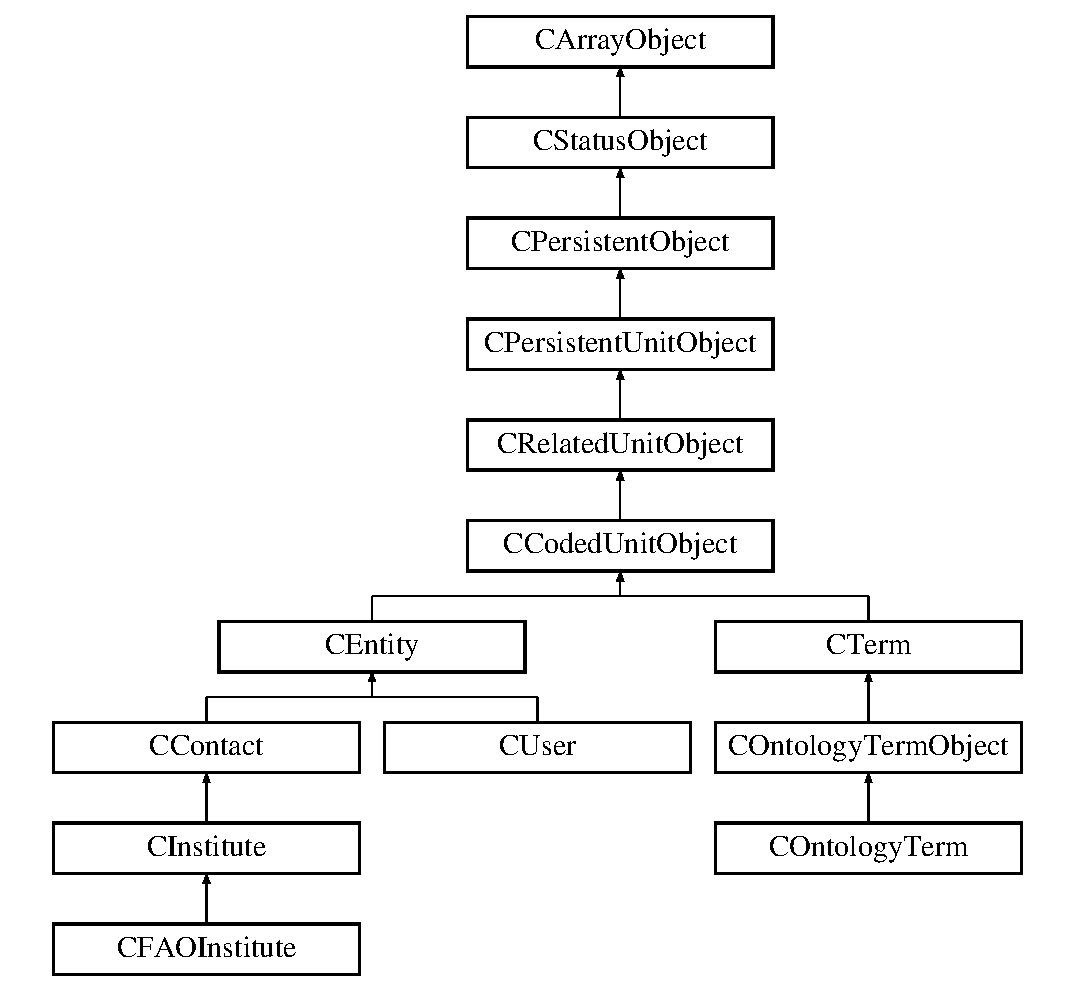
\includegraphics[height=9.655172cm]{class_c_related_unit_object}
\end{center}
\end{figure}
\subsection*{Public Member Functions}
\begin{DoxyCompactItemize}
\item 
\hyperlink{class_c_related_unit_object_a46a7033129ae23ecda7f879f3fabdd5c}{Relate} (\$the\-Object, \$the\-Predicate=N\-U\-L\-L, \$the\-Operation=N\-U\-L\-L, \$get\-Old=F\-A\-L\-S\-E)
\item 
\hyperlink{class_c_related_unit_object_a6f19ef5d6eb0414712a16919e0ef3d5d}{Used} (\$the\-Value=N\-U\-L\-L, \$get\-Old=F\-A\-L\-S\-E)
\item 
\hyperlink{class_c_related_unit_object_a5f4a93894d26ead9fe1b80e39975ec12}{Preferred} (\$the\-Value=N\-U\-L\-L, \$get\-Old=F\-A\-L\-S\-E)
\item 
\hyperlink{class_c_related_unit_object_aea51a443754ab8c86a23ece7a2b18b1f}{Valid} (\$the\-Value=N\-U\-L\-L, \$get\-Old=F\-A\-L\-S\-E)
\end{DoxyCompactItemize}
\subsection*{Static Public Member Functions}
\begin{DoxyCompactItemize}
\item 
static \hyperlink{class_c_related_unit_object_ac170015e2540be0c038a4cb2821add8c}{Valid\-Object} (\$the\-Container, \$the\-Identifier, \$the\-Modifiers=k\-F\-L\-A\-G\-\_\-\-D\-E\-F\-A\-U\-L\-T)
\end{DoxyCompactItemize}
\subsection*{Protected Member Functions}
\begin{DoxyCompactItemize}
\item 
\hyperlink{class_c_related_unit_object_a577c73999830641e07440126a3252286}{\-\_\-\-Prepare\-Commit} (\&\$the\-Container, \&\$the\-Identifier, \&\$the\-Modifiers)
\end{DoxyCompactItemize}
\subsection*{Additional Inherited Members}


\subsection{Member Function Documentation}
\hypertarget{class_c_related_unit_object_a577c73999830641e07440126a3252286}{\index{C\-Related\-Unit\-Object@{C\-Related\-Unit\-Object}!\-\_\-\-Prepare\-Commit@{\-\_\-\-Prepare\-Commit}}
\index{\-\_\-\-Prepare\-Commit@{\-\_\-\-Prepare\-Commit}!CRelatedUnitObject@{C\-Related\-Unit\-Object}}
\subsubsection[{\-\_\-\-Prepare\-Commit}]{\setlength{\rightskip}{0pt plus 5cm}C\-Related\-Unit\-Object\-::\-\_\-\-Prepare\-Commit (
\begin{DoxyParamCaption}
\item[{\&}]{\$the\-Container, }
\item[{\&}]{\$the\-Identifier, }
\item[{\&}]{\$the\-Modifiers}
\end{DoxyParamCaption}
)\hspace{0.3cm}{\ttfamily [protected]}}}\label{class_c_related_unit_object_a577c73999830641e07440126a3252286}
Normalise before a store.

We \hyperlink{class_c_persistent_unit_object_aaa69a5dd56c441027197d5cb677972ad}{overload} this method to \hyperlink{class_c_persistent_object_a88b1f2b11d3d60e0b3d33d8b0649b68a}{commit} eventual object references stored as instances. We scan the \hyperlink{class_c_related_unit_object_a46a7033129ae23ecda7f879f3fabdd5c}{relations} and the \hyperlink{class_c_related_unit_object_aea51a443754ab8c86a23ece7a2b18b1f}{valid} references and process all elements that derive from this class.


\begin{DoxyParams}[1]{Parameters}
reference & {\em \&\$the\-Container} & Object container. \\
\hline
reference & {\em \&\$the\-Identifier} & Object identifier. \\
\hline
reference & {\em \&\$the\-Modifiers} & Commit modifiers.\\
\hline
\end{DoxyParams}
protected


\begin{DoxyExceptions}{Exceptions}
{\em \{@link} & \hyperlink{class_c_exception}{C\-Exception} \hyperlink{class_c_exception}{C\-Exception}\}\\
\hline
\end{DoxyExceptions}
\begin{DoxySeeAlso}{See Also}
k\-E\-R\-R\-O\-R\-\_\-\-O\-P\-T\-I\-O\-N\-\_\-\-M\-I\-S\-S\-I\-N\-G 
\end{DoxySeeAlso}


Reimplemented from \hyperlink{class_c_persistent_unit_object_aaa69a5dd56c441027197d5cb677972ad}{C\-Persistent\-Unit\-Object}.



Reimplemented in \hyperlink{class_c_ontology_term_a5d10f6baf1e484591d1d99b325e22d89}{C\-Ontology\-Term}, \hyperlink{class_c_ontology_term_object_aca3572974abb180f507fc63264a9ba15}{C\-Ontology\-Term\-Object}, \hyperlink{class_c_dataset_aaa2f58e75510697834f905e434bfb3aa}{C\-Dataset}, \hyperlink{class_c_f_a_o_institute_a9917150b0e31b741aa10c9443e880746}{C\-F\-A\-O\-Institute}, \hyperlink{class_c_ontology_tag_a8f4f23a880ee224c8d154ed81fdd5d94}{C\-Ontology\-Tag}, \hyperlink{class_c_user_aacdc43c5a38cb6b013ee9ce686b186e9}{C\-User}, \hyperlink{class_c_institute_a096aa38309ae2f88250700d5755a18a6}{C\-Institute}, and \hyperlink{class_c_entity_ac306808f0f8404fa405674cbe14fd441}{C\-Entity}.

\hypertarget{class_c_related_unit_object_a5f4a93894d26ead9fe1b80e39975ec12}{\index{C\-Related\-Unit\-Object@{C\-Related\-Unit\-Object}!Preferred@{Preferred}}
\index{Preferred@{Preferred}!CRelatedUnitObject@{C\-Related\-Unit\-Object}}
\subsubsection[{Preferred}]{\setlength{\rightskip}{0pt plus 5cm}C\-Related\-Unit\-Object\-::\-Preferred (
\begin{DoxyParamCaption}
\item[{}]{\$the\-Value = {\ttfamily NULL}, }
\item[{}]{\$get\-Old = {\ttfamily FALSE}}
\end{DoxyParamCaption}
)}}\label{class_c_related_unit_object_a5f4a93894d26ead9fe1b80e39975ec12}
Manage used reference.

This method can be used to handle the object's preferred reference, it uses the standard accessor \hyperlink{class_c_attribute_a9d231a47718719fcd6c33f3d0ac91675}{method} to manage the \hyperlink{}{offset}.

Objects may become obsolete, but still represent valid entries\-: in this case we use this attribute to point to the preferred object.

For a more in-\/depth reference of this method, please consult the \hyperlink{class_c_attribute_a9d231a47718719fcd6c33f3d0ac91675}{C\-Attribute\-::\-Manage\-Offset} method, in which the second parameter will be the constant \hyperlink{}{k\-T\-A\-G\-\_\-\-P\-R\-E\-F\-E\-R\-R\-E\-D}.

In this class we feed the value to the \hyperlink{class_c_persistent_unit_object_abdf69880df0ce8257c4d0fd64adc7053}{Normalise\-Related\-Object} method that will take care of handling object references.


\begin{DoxyParams}[1]{Parameters}
mixed & {\em \$the\-Value} & Value. \\
\hline
boolean & {\em \$get\-Old} & T\-R\-U\-E get old value.\\
\hline
\end{DoxyParams}
public \begin{DoxyReturn}{Returns}
string
\end{DoxyReturn}
\hyperlink{class_c_attribute_a9d231a47718719fcd6c33f3d0ac91675}{C\-Attribute\-::\-Manage\-Offset()}

\begin{DoxySeeAlso}{See Also}
k\-T\-A\-G\-\_\-\-P\-R\-E\-F\-E\-R\-R\-E\-D 
\end{DoxySeeAlso}
\hypertarget{class_c_related_unit_object_a46a7033129ae23ecda7f879f3fabdd5c}{\index{C\-Related\-Unit\-Object@{C\-Related\-Unit\-Object}!Relate@{Relate}}
\index{Relate@{Relate}!CRelatedUnitObject@{C\-Related\-Unit\-Object}}
\subsubsection[{Relate}]{\setlength{\rightskip}{0pt plus 5cm}C\-Related\-Unit\-Object\-::\-Relate (
\begin{DoxyParamCaption}
\item[{}]{\$the\-Object, }
\item[{}]{\$the\-Predicate = {\ttfamily NULL}, }
\item[{}]{\$the\-Operation = {\ttfamily NULL}, }
\item[{}]{\$get\-Old = {\ttfamily FALSE}}
\end{DoxyParamCaption}
)}}\label{class_c_related_unit_object_a46a7033129ae23ecda7f879f3fabdd5c}
Manage object references.

This method can be used to manage relationships between the current object and other objects, it is represented as a list of subject/predicate/object relationships in which the subject is the current object, and the list of predicate/object pairs will be stored in the \hyperlink{}{k\-T\-A\-G\-\_\-\-R\-E\-F\-S} offset.

The method accepts the following parameters\-:


\begin{DoxyItemize}
\item {\bfseries \$the\-Object}\-: Relation object, it should either be the relation object itself, or an object reference to the relation's object. Before the current object is \hyperlink{class_c_persistent_object_a88b1f2b11d3d60e0b3d33d8b0649b68a}{committed}, all elements provided as instances derived from the \hyperlink{class_c_related_unit_object}{C\-Related\-Unit\-Object} class will also be \hyperlink{class_c_persistent_unit_object_ae74127a9fb936d8cf5aeed30315ac05b}{committed} and converted to object references. This parameter is passed through a protected \hyperlink{class_c_persistent_unit_object_abdf69880df0ce8257c4d0fd64adc7053}{method} that derived classes can use to validate and normalise relation objects. 
\item {\bfseries \$the\-Predicate}\-: Relation predicate, this parameter represents the kind or predicate of the relation, depending on whether it is provided or not, each element of the relations list will take the following form\-: 
\begin{DoxyItemize}
\item {\itshape N\-U\-L\-L}\-: If the predicate is omitted, the element of the relation will only have the object parameter. 
\item {\itshape F\-A\-L\-S\-E} The element will be an array composed of one element, \hyperlink{}{k\-T\-A\-G\-\_\-\-D\-A\-T\-A}, which will hold the firat parameter. 
\item {\itshape other} The element will be an array composed of two elements\-: 
\begin{DoxyItemize}
\item {\itshape \hyperlink{}{k\-T\-A\-G\-\_\-\-K\-I\-N\-D}}\-: This offset represents the reference predicate, it will hold the value of this parameter. 
\item {\itshape \hyperlink{}{k\-T\-A\-G\-\_\-\-D\-A\-T\-A}}\-: This offset represents the reference object, it will hold the value of the first parameter. 
\end{DoxyItemize}This parameter is passed through a protected \hyperlink{class_c_persistent_unit_object_ad9c886156b37fa09552de223b1efddd6}{method} that derived classes can use to validate and normalise relation predicates. 
\end{DoxyItemize}
\item {\bfseries \$the\-Operation}\-: The operation to perform\-: 
\begin{DoxyItemize}
\item {\itshape N\-U\-L\-L}\-: Return the element matched by the previous parameters. 
\item {\itshape F\-A\-L\-S\-E}\-: Delete the element matched by the previous parameters and return it. 
\item {\itshape other}\-: Any other value means that we want to add to the list the element provided in the previous parameters, either appending it if there was no matching element, or by replacing a matching element. The method will return either the replaced element or the new one. 
\end{DoxyItemize}
\item {\bfseries \$get\-Old}\-: Determines what the method will return when deleting or replacing\-: 
\begin{DoxyItemize}
\item {\itshape T\-R\-U\-E}\-: Return the deleted or replaced element. 
\item {\itshape F\-A\-L\-S\-E}\-: Return the replacing element or {\itshape N\-U\-L\-L} when deleting. 
\end{DoxyItemize}
\end{DoxyItemize}


\begin{DoxyParams}[1]{Parameters}
mixed & {\em \$the\-Object} & Reference object. \\
\hline
mixed & {\em \$the\-Predicate} & Reference predicate. \\
\hline
mixed & {\em \$the\-Operation} & Operation. \\
\hline
boolean & {\em \$get\-Old} & T\-R\-U\-E get old value.\\
\hline
\end{DoxyParams}
public \begin{DoxyReturn}{Returns}
mixed
\end{DoxyReturn}
\hyperlink{class_c_persistent_unit_object_abdf69880df0ce8257c4d0fd64adc7053}{C\-Persistent\-Unit\-Object\-::\-Normalise\-Related\-Object()}  \hyperlink{class_c_persistent_unit_object_ad9c886156b37fa09552de223b1efddd6}{C\-Persistent\-Unit\-Object\-::\-Normalise\-Related\-Predicate()}  \hyperlink{class_c_attribute_a58d5de30d4a6ea29f485a266460a2bdd}{C\-Attribute\-::\-Manage\-Object\-List()}

\begin{DoxySeeAlso}{See Also}
k\-T\-A\-G\-\_\-\-R\-E\-F\-S k\-T\-A\-G\-\_\-\-K\-I\-N\-D k\-T\-A\-G\-\_\-\-D\-A\-T\-A 
\end{DoxySeeAlso}


Reimplemented in \hyperlink{class_c_ontology_term_a47a361f6634f8e1df8186571a350711e}{C\-Ontology\-Term}.

\hypertarget{class_c_related_unit_object_a6f19ef5d6eb0414712a16919e0ef3d5d}{\index{C\-Related\-Unit\-Object@{C\-Related\-Unit\-Object}!Used@{Used}}
\index{Used@{Used}!CRelatedUnitObject@{C\-Related\-Unit\-Object}}
\subsubsection[{Used}]{\setlength{\rightskip}{0pt plus 5cm}C\-Related\-Unit\-Object\-::\-Used (
\begin{DoxyParamCaption}
\item[{}]{\$the\-Value = {\ttfamily NULL}, }
\item[{}]{\$get\-Old = {\ttfamily FALSE}}
\end{DoxyParamCaption}
)}}\label{class_c_related_unit_object_a6f19ef5d6eb0414712a16919e0ef3d5d}
Manage used reference.

This method can be used to handle the object's default reference, it uses the standard accessor \hyperlink{class_c_attribute_a9d231a47718719fcd6c33f3d0ac91675}{method} to manage the \hyperlink{}{offset}.

In enumerations, for instance, there may be several entries that refer to a single entity\-: this tag should be used to point to the instance that represents the used or default choice.

For a more in-\/depth reference of this method, please consult the \hyperlink{class_c_attribute_a9d231a47718719fcd6c33f3d0ac91675}{C\-Attribute\-::\-Manage\-Offset} method, in which the second parameter will be the constant \hyperlink{}{k\-T\-A\-G\-\_\-\-D\-E\-F\-A\-U\-L\-T}.

In this class we feed the value to the \hyperlink{class_c_persistent_unit_object_abdf69880df0ce8257c4d0fd64adc7053}{Normalise\-Related\-Object} method that will take care of handling object references.


\begin{DoxyParams}[1]{Parameters}
mixed & {\em \$the\-Value} & Value. \\
\hline
boolean & {\em \$get\-Old} & T\-R\-U\-E get old value.\\
\hline
\end{DoxyParams}
public \begin{DoxyReturn}{Returns}
string
\end{DoxyReturn}
\hyperlink{class_c_attribute_a9d231a47718719fcd6c33f3d0ac91675}{C\-Attribute\-::\-Manage\-Offset()}

\begin{DoxySeeAlso}{See Also}
k\-T\-A\-G\-\_\-\-D\-E\-F\-A\-U\-L\-T 
\end{DoxySeeAlso}
\hypertarget{class_c_related_unit_object_aea51a443754ab8c86a23ece7a2b18b1f}{\index{C\-Related\-Unit\-Object@{C\-Related\-Unit\-Object}!Valid@{Valid}}
\index{Valid@{Valid}!CRelatedUnitObject@{C\-Related\-Unit\-Object}}
\subsubsection[{Valid}]{\setlength{\rightskip}{0pt plus 5cm}C\-Related\-Unit\-Object\-::\-Valid (
\begin{DoxyParamCaption}
\item[{}]{\$the\-Value = {\ttfamily NULL}, }
\item[{}]{\$get\-Old = {\ttfamily FALSE}}
\end{DoxyParamCaption}
)}}\label{class_c_related_unit_object_aea51a443754ab8c86a23ece7a2b18b1f}
Manage valid reference.

This method can be used to handle the valid object's \hyperlink{}{identifier}, it uses the standard accessor \hyperlink{class_c_attribute_a9d231a47718719fcd6c33f3d0ac91675}{method} to manage the \hyperlink{}{offset}.

Objects derived from this class should be persistent, in other words, it is not an option to delete such objects\-: by creating a new object and referencing it from the old one, we maintain the original reference and point to the valid object.

For a more in-\/depth reference of this method, please consult the \hyperlink{class_c_attribute_a9d231a47718719fcd6c33f3d0ac91675}{C\-Attribute\-::\-Manage\-Offset} method, in which the second parameter will be the constant \hyperlink{}{k\-T\-A\-G\-\_\-\-V\-A\-L\-I\-D}.

In this class we feed the value to the \hyperlink{class_c_persistent_unit_object_abdf69880df0ce8257c4d0fd64adc7053}{Normalise\-Related\-Object} method that will take care of handling object references.


\begin{DoxyParams}[1]{Parameters}
mixed & {\em \$the\-Value} & Value. \\
\hline
boolean & {\em \$get\-Old} & T\-R\-U\-E get old value.\\
\hline
\end{DoxyParams}
public \begin{DoxyReturn}{Returns}
string
\end{DoxyReturn}
\hyperlink{class_c_attribute_a9d231a47718719fcd6c33f3d0ac91675}{C\-Attribute\-::\-Manage\-Offset()}

\begin{DoxySeeAlso}{See Also}
k\-T\-A\-G\-\_\-\-V\-A\-L\-I\-D 
\end{DoxySeeAlso}


Reimplemented in \hyperlink{class_c_ontology_term_a926d7b17908b252e584343db52bb9a45}{C\-Ontology\-Term}.

\hypertarget{class_c_related_unit_object_ac170015e2540be0c038a4cb2821add8c}{\index{C\-Related\-Unit\-Object@{C\-Related\-Unit\-Object}!Valid\-Object@{Valid\-Object}}
\index{Valid\-Object@{Valid\-Object}!CRelatedUnitObject@{C\-Related\-Unit\-Object}}
\subsubsection[{Valid\-Object}]{\setlength{\rightskip}{0pt plus 5cm}static C\-Related\-Unit\-Object\-::\-Valid\-Object (
\begin{DoxyParamCaption}
\item[{}]{\$the\-Container, }
\item[{}]{\$the\-Identifier, }
\item[{}]{\$the\-Modifiers = {\ttfamily kFLAG\-\_\-DEFAULT}}
\end{DoxyParamCaption}
)\hspace{0.3cm}{\ttfamily [static]}}}\label{class_c_related_unit_object_ac170015e2540be0c038a4cb2821add8c}
Return a valid object.

This method can be used to instantiate a valid object, this means that if we provide the identifier of an expired or obsolete object that has a reference to a \hyperlink{class_c_related_unit_object_aea51a443754ab8c86a23ece7a2b18b1f}{valid} object, this method will return the valid one.

The method expects the same parameters as the \hyperlink{class_c_persistent_unit_object_ab3e33158e9b08a45f3a0b71feb922f50}{New\-Object} static method. If the \hyperlink{class_c_related_unit_object_aea51a443754ab8c86a23ece7a2b18b1f}{valid} chain is recursive, the method will raise an exception.

The method will return the first object that does not have a \hyperlink{class_c_related_unit_object_aea51a443754ab8c86a23ece7a2b18b1f}{valid} \hyperlink{}{reference}, or {\itshape N\-U\-L\-L} if the object was not found.


\begin{DoxyParams}[1]{Parameters}
mixed & {\em \$the\-Container} & Persistent container. \\
\hline
mixed & {\em \$the\-Identifier} & Object identifier. \\
\hline
bitfield & {\em \$the\-Modifiers} & Load modifiers.\\
\hline
\end{DoxyParams}
\begin{DoxyReturn}{Returns}
C\-Graph\-Node\-Object 
\end{DoxyReturn}


Reimplemented in \hyperlink{class_c_ontology_term_a2372abc77a54330f60447a196db1ee7f}{C\-Ontology\-Term}.



The documentation for this class was generated from the following file\-:\begin{DoxyCompactItemize}
\item 
/\-Library/\-Web\-Server/\-Library/wrapper/classes/C\-Related\-Unit\-Object.\-php\end{DoxyCompactItemize}

\hypertarget{class_c_status_object}{\section{C\-Status\-Object Class Reference}
\label{class_c_status_object}\index{C\-Status\-Object@{C\-Status\-Object}}
}
Inheritance diagram for C\-Status\-Object\-:\begin{figure}[H]
\begin{center}
\leavevmode
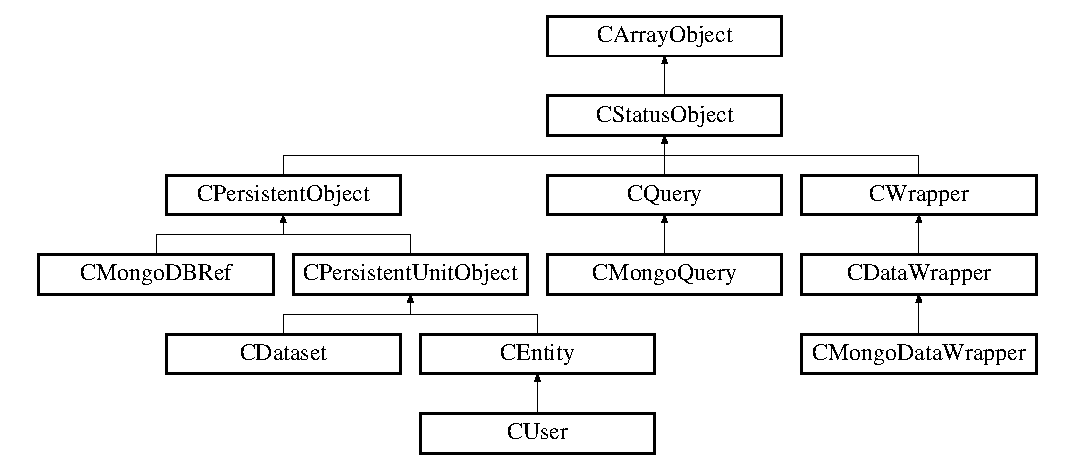
\includegraphics[height=4.000000cm]{class_c_status_object}
\end{center}
\end{figure}
\subsection*{Public Member Functions}
\begin{DoxyCompactItemize}
\item 
\hyperlink{class_c_status_object_a140ef140d4fa1c4a6180e843bd5ec969}{offset\-Set} (\$the\-Offset, \$the\-Value)
\item 
\hyperlink{class_c_status_object_ae733db1bbfffcbe894ea405765ab4150}{offset\-Unset} (\$the\-Offset)
\item 
\hyperlink{class_c_status_object_a6c68cf419c07a3af8ef7e83690590235}{Status} (\$the\-State=N\-U\-L\-L)
\end{DoxyCompactItemize}
\subsection*{Protected Member Functions}
\begin{DoxyCompactItemize}
\item 
\hyperlink{class_c_status_object_a8429102e4f52f7558649b64f4e673a69}{\-\_\-\-Is\-Inited} (\$the\-State=N\-U\-L\-L)
\item 
\hyperlink{class_c_status_object_a19c4ac94dfe26476e780d77b99744d43}{\-\_\-\-Is\-Dirty} (\$the\-State=N\-U\-L\-L)
\item 
\hyperlink{class_c_status_object_a3e37d72a6462d93bf7ff567f07f78093}{\-\_\-\-Manage\-Bit\-Field} (\&\$the\-Field, \$the\-Mask, \$the\-State=N\-U\-L\-L)
\end{DoxyCompactItemize}
\subsection*{Protected Attributes}
\begin{DoxyCompactItemize}
\item 
\hypertarget{class_c_status_object_af80d790146175e2f634d1b84ead1161b}{{\bfseries \$m\-Status} = k\-F\-L\-A\-G\-\_\-\-D\-E\-F\-A\-U\-L\-T}\label{class_c_status_object_af80d790146175e2f634d1b84ead1161b}

\end{DoxyCompactItemize}


\subsection{Member Function Documentation}
\hypertarget{class_c_status_object_a19c4ac94dfe26476e780d77b99744d43}{\index{C\-Status\-Object@{C\-Status\-Object}!\-\_\-\-Is\-Dirty@{\-\_\-\-Is\-Dirty}}
\index{\-\_\-\-Is\-Dirty@{\-\_\-\-Is\-Dirty}!CStatusObject@{C\-Status\-Object}}
\subsubsection[{\-\_\-\-Is\-Dirty}]{\setlength{\rightskip}{0pt plus 5cm}C\-Status\-Object\-::\-\_\-\-Is\-Dirty (
\begin{DoxyParamCaption}
\item[{}]{\$the\-State = {\ttfamily NULL}}
\end{DoxyParamCaption}
)\hspace{0.3cm}{\ttfamily [protected]}}}\label{class_c_status_object_a19c4ac94dfe26476e780d77b99744d43}
Manage dirty status.

This method can be used to get or set the object's dirty state.

A dirty object is one that was modified since the last time this state was probed. In general, this state should be set whenever the persistent properties of the object are modified.

In this class we automatically set this state when \hyperlink{class_c_status_object_a140ef140d4fa1c4a6180e843bd5ec969}{setting} or \hyperlink{class_c_status_object_ae733db1bbfffcbe894ea405765ab4150}{deleting} array store elements.

The method features a single parameter\-:


\begin{DoxyItemize}
\item {\itshape N\-U\-L\-L}\-: The method will return {\itshape T\-R\-U\-E} if the object is dirty, or {\itshape F\-A\-L\-S\-E} if the object is \hyperlink{}{clean}. 
\item {\itshape T\-R\-U\-E}\-: The method will set the object to dirty. 
\item {\itshape F\-A\-L\-S\-E}\-: The method will set the object to \hyperlink{}{clean}. 
\end{DoxyItemize}

In all cases the method will return the state {\itshape after} it was eventually modified.


\begin{DoxyParams}[1]{Parameters}
mixed & {\em \$the\-State} & T\-R\-U\-E, F\-A\-L\-S\-E or N\-U\-L\-L.\\
\hline
\end{DoxyParams}
protected \begin{DoxyReturn}{Returns}
boolean
\end{DoxyReturn}
\hyperlink{class_c_status_object_a3e37d72a6462d93bf7ff567f07f78093}{\-\_\-\-Manage\-Bit\-Field()}

\begin{DoxySeeAlso}{See Also}
k\-F\-L\-A\-G\-\_\-\-S\-T\-A\-T\-E\-\_\-\-D\-I\-R\-T\-Y 
\end{DoxySeeAlso}
\hypertarget{class_c_status_object_a8429102e4f52f7558649b64f4e673a69}{\index{C\-Status\-Object@{C\-Status\-Object}!\-\_\-\-Is\-Inited@{\-\_\-\-Is\-Inited}}
\index{\-\_\-\-Is\-Inited@{\-\_\-\-Is\-Inited}!CStatusObject@{C\-Status\-Object}}
\subsubsection[{\-\_\-\-Is\-Inited}]{\setlength{\rightskip}{0pt plus 5cm}C\-Status\-Object\-::\-\_\-\-Is\-Inited (
\begin{DoxyParamCaption}
\item[{}]{\$the\-State = {\ttfamily NULL}}
\end{DoxyParamCaption}
)\hspace{0.3cm}{\ttfamily [protected]}}}\label{class_c_status_object_a8429102e4f52f7558649b64f4e673a69}
Manage inited status.

This method can be used to get or set the object's inited state.

An object becomes inited when it has all the required elements necessary for it to be correctly used or persistently stored. Such a state indicates that at least the minimum required information was initialised in the object.

The counterpart state indicates that the object still lacks the necessary elements to successfully operate the object.

This method operates by setting or clearing the \hyperlink{}{inited} \hyperlink{class_c_status_object_a6c68cf419c07a3af8ef7e83690590235}{status} flag.

The method features a single parameter\-:


\begin{DoxyItemize}
\item {\itshape N\-U\-L\-L}\-: The method will return {\itshape T\-R\-U\-E} if the object is this state, or {\itshape F\-A\-L\-S\-E} if the object is not in this state. 
\item {\itshape T\-R\-U\-E}\-: The method will set the object to this state. 
\item {\itshape F\-A\-L\-S\-E}\-: The method will reset this state. 
\end{DoxyItemize}

In all cases the method will return the state {\itshape after} it was eventually modified.


\begin{DoxyParams}[1]{Parameters}
mixed & {\em \$the\-State} & T\-R\-U\-E, F\-A\-L\-S\-E or N\-U\-L\-L.\\
\hline
\end{DoxyParams}
protected \begin{DoxyReturn}{Returns}
boolean
\end{DoxyReturn}
\hyperlink{class_c_status_object_a3e37d72a6462d93bf7ff567f07f78093}{\-\_\-\-Manage\-Bit\-Field()}

\begin{DoxySeeAlso}{See Also}
k\-F\-L\-A\-G\-\_\-\-S\-T\-A\-T\-E\-\_\-\-I\-N\-I\-T\-E\-D 
\end{DoxySeeAlso}
\hypertarget{class_c_status_object_a3e37d72a6462d93bf7ff567f07f78093}{\index{C\-Status\-Object@{C\-Status\-Object}!\-\_\-\-Manage\-Bit\-Field@{\-\_\-\-Manage\-Bit\-Field}}
\index{\-\_\-\-Manage\-Bit\-Field@{\-\_\-\-Manage\-Bit\-Field}!CStatusObject@{C\-Status\-Object}}
\subsubsection[{\-\_\-\-Manage\-Bit\-Field}]{\setlength{\rightskip}{0pt plus 5cm}C\-Status\-Object\-::\-\_\-\-Manage\-Bit\-Field (
\begin{DoxyParamCaption}
\item[{\&}]{\$the\-Field, }
\item[{}]{\$the\-Mask, }
\item[{}]{\$the\-State = {\ttfamily NULL}}
\end{DoxyParamCaption}
)\hspace{0.3cm}{\ttfamily [protected]}}}\label{class_c_status_object_a3e37d72a6462d93bf7ff567f07f78093}
Manage bit-\/field property.

This method can be used to manage a bitfield property, it accepts the following parameters\-:


\begin{DoxyItemize}
\item {\bfseries \&\$the\-Field}\-: Reference to the bit-\/field property. 
\item {\bfseries \$the\-Mask}\-: Bit-\/field mask. 
\item {\bfseries \$the\-State}\-: State or operator\-: 
\begin{DoxyItemize}
\item {\itshape N\-U\-L\-L}\-: Return the current value masked by the next parameter. 
\item {\itshape F\-A\-L\-S\-E}\-: Reset the current value using the next parameter as the mask. 
\item {\itshape other}\-: Set the current value to this one, masking the first 31 bits. 
\end{DoxyItemize}
\end{DoxyItemize}

In all cases the method will return the status {\itshape after} it was eventually modified.


\begin{DoxyParams}[1]{Parameters}
reference & {\em \&\$the\-Field} & Bit-\/field reference. \\
\hline
bitfield & {\em \$the\-Mask} & Bit-\/field mask. \\
\hline
mixed & {\em \$the\-State} & Value or operator.\\
\hline
\end{DoxyParams}
protected \begin{DoxyReturn}{Returns}
bitfield
\end{DoxyReturn}
\begin{DoxySeeAlso}{See Also}
k\-F\-L\-A\-G\-\_\-\-D\-E\-F\-A\-U\-L\-T\-\_\-\-M\-A\-S\-K 
\end{DoxySeeAlso}
\hypertarget{class_c_status_object_a140ef140d4fa1c4a6180e843bd5ec969}{\index{C\-Status\-Object@{C\-Status\-Object}!offset\-Set@{offset\-Set}}
\index{offset\-Set@{offset\-Set}!CStatusObject@{C\-Status\-Object}}
\subsubsection[{offset\-Set}]{\setlength{\rightskip}{0pt plus 5cm}C\-Status\-Object\-::offset\-Set (
\begin{DoxyParamCaption}
\item[{}]{\$the\-Offset, }
\item[{}]{\$the\-Value}
\end{DoxyParamCaption}
)}}\label{class_c_status_object_a140ef140d4fa1c4a6180e843bd5ec969}
Set a value for a given offset.

We override this method to handle the \hyperlink{class_c_status_object_a19c4ac94dfe26476e780d77b99744d43}{dirty} \hyperlink{}{flag}\-: on offset value changes we set the state on.


\begin{DoxyParams}[1]{Parameters}
string & {\em \$the\-Offset} & Offset. \\
\hline
string | N\-U\-L\-L & {\em \$the\-Value} & Value to set at offset.\\
\hline
\end{DoxyParams}
public

\hyperlink{class_c_status_object_a19c4ac94dfe26476e780d77b99744d43}{\-\_\-\-Is\-Dirty()}

\begin{DoxySeeAlso}{See Also}
k\-F\-L\-A\-G\-\_\-\-S\-T\-A\-T\-E\-\_\-\-D\-I\-R\-T\-Y 
\end{DoxySeeAlso}


Reimplemented from \hyperlink{class_c_array_object_a41815b543b14d373f68ed34ca53dc9f6}{C\-Array\-Object}.



Reimplemented in \hyperlink{class_c_ontology_term_aba486e72f54e61651a75da75215aaa7c}{C\-Ontology\-Term}, \hyperlink{class_c_dataset_a72f36837282a754ba453799172802e31}{C\-Dataset}, \hyperlink{class_c_wrapper_client_ac37ea353c211b696d11e103a069e8633}{C\-Wrapper\-Client}, \hyperlink{class_c_graph_node_acf4f4240a7807ff16d81378aa282595c}{C\-Graph\-Node}, \hyperlink{class_c_user_aace3446b9cacfe28cc1937c608fcc999}{C\-User}, \hyperlink{class_c_institute_a16c349e22775161c89dbf73850b24cd7}{C\-Institute}, \hyperlink{class_c_f_a_o_institute_ac819c5bfa381ffa0f78b34442d2ea3c2}{C\-F\-A\-O\-Institute}, and \hyperlink{class_c_coded_unit_object_a49bb8f2956cb0551ba827b222778f295}{C\-Coded\-Unit\-Object}.

\hypertarget{class_c_status_object_ae733db1bbfffcbe894ea405765ab4150}{\index{C\-Status\-Object@{C\-Status\-Object}!offset\-Unset@{offset\-Unset}}
\index{offset\-Unset@{offset\-Unset}!CStatusObject@{C\-Status\-Object}}
\subsubsection[{offset\-Unset}]{\setlength{\rightskip}{0pt plus 5cm}C\-Status\-Object\-::offset\-Unset (
\begin{DoxyParamCaption}
\item[{}]{\$the\-Offset}
\end{DoxyParamCaption}
)}}\label{class_c_status_object_ae733db1bbfffcbe894ea405765ab4150}
Reset a value for a given offset.

We override this method to handle the \hyperlink{class_c_status_object_a19c4ac94dfe26476e780d77b99744d43}{dirty} \hyperlink{}{flag}\-: on offset value changes we set the state on.


\begin{DoxyParams}[1]{Parameters}
string & {\em \$the\-Offset} & Offset.\\
\hline
\end{DoxyParams}
public

\hyperlink{class_c_status_object_a19c4ac94dfe26476e780d77b99744d43}{\-\_\-\-Is\-Dirty()}

\begin{DoxySeeAlso}{See Also}
k\-F\-L\-A\-G\-\_\-\-S\-T\-A\-T\-E\-\_\-\-D\-I\-R\-T\-Y 
\end{DoxySeeAlso}


Reimplemented from \hyperlink{class_c_array_object_a2852b78f58379e507b5e7d7cb8e5326b}{C\-Array\-Object}.



Reimplemented in \hyperlink{class_c_ontology_term_a622c31b9466e49a1413d38fda9ef9bb1}{C\-Ontology\-Term}, \hyperlink{class_c_dataset_a9f048a8cbe7109da16a8ef2b7cbd2165}{C\-Dataset}, \hyperlink{class_c_graph_node_aab1d86d6dda1fffa9dd515b23851588a}{C\-Graph\-Node}, \hyperlink{class_c_wrapper_client_af4a349c007923b1229f3099592660d97}{C\-Wrapper\-Client}, \hyperlink{class_c_user_aed8557e18a89d868cedf5a48328b33b2}{C\-User}, \hyperlink{class_c_institute_a8f82ded3b52a6fb609c67e45669e1454}{C\-Institute}, \hyperlink{class_c_f_a_o_institute_a3bd7c59a3da53ba8c3cd1d9d0ff5ae0a}{C\-F\-A\-O\-Institute}, and \hyperlink{class_c_coded_unit_object_a5072e0f72c19260df212a4cf93c9f1cb}{C\-Coded\-Unit\-Object}.

\hypertarget{class_c_status_object_a6c68cf419c07a3af8ef7e83690590235}{\index{C\-Status\-Object@{C\-Status\-Object}!Status@{Status}}
\index{Status@{Status}!CStatusObject@{C\-Status\-Object}}
\subsubsection[{Status}]{\setlength{\rightskip}{0pt plus 5cm}C\-Status\-Object\-::\-Status (
\begin{DoxyParamCaption}
\item[{}]{\$the\-State = {\ttfamily NULL}}
\end{DoxyParamCaption}
)}}\label{class_c_status_object_a6c68cf419c07a3af8ef7e83690590235}
Set or retrieve the object status.

This method can be used to manage the status bitfield as a whole, allowing to set and retrieve the whole set of states.

The parameter can take the following values\-:


\begin{DoxyItemize}
\item {\itshape N\-U\-L\-L}\-: The method will return the current object's states bitfield. 
\item {\itshape F\-A\-L\-S\-E}\-: If this value is passed, the method will reset the object's status by settig it to the \hyperlink{}{default} value. 
\item {\itshape other}\-: In this case the parameter will be interpreted as a 31 bits bit-\/field value and the data member will be replaced with it. 
\end{DoxyItemize}

In all cases the method will return the status {\itshape after} it was eventually modified.


\begin{DoxyParams}[1]{Parameters}
N\-U\-L\-L | F\-A\-L\-S\-E | bitfield & {\em \$the\-State} & N\-U\-L\-L, F\-A\-L\-S\-E or new status.\\
\hline
\end{DoxyParams}
public \begin{DoxyReturn}{Returns}
bitfield
\end{DoxyReturn}
\hyperlink{class_c_status_object_a3e37d72a6462d93bf7ff567f07f78093}{\-\_\-\-Manage\-Bit\-Field()}

\begin{DoxySeeAlso}{See Also}
k\-F\-L\-A\-G\-\_\-\-D\-E\-F\-A\-U\-L\-T\-\_\-\-M\-A\-S\-K 
\end{DoxySeeAlso}


The documentation for this class was generated from the following file\-:\begin{DoxyCompactItemize}
\item 
/\-Library/\-Web\-Server/\-Library/wrapper/classes/C\-Status\-Object.\-php\end{DoxyCompactItemize}

\hypertarget{class_c_term}{\section{C\-Term Class Reference}
\label{class_c_term}\index{C\-Term@{C\-Term}}
}
Inheritance diagram for C\-Term\-:\begin{figure}[H]
\begin{center}
\leavevmode
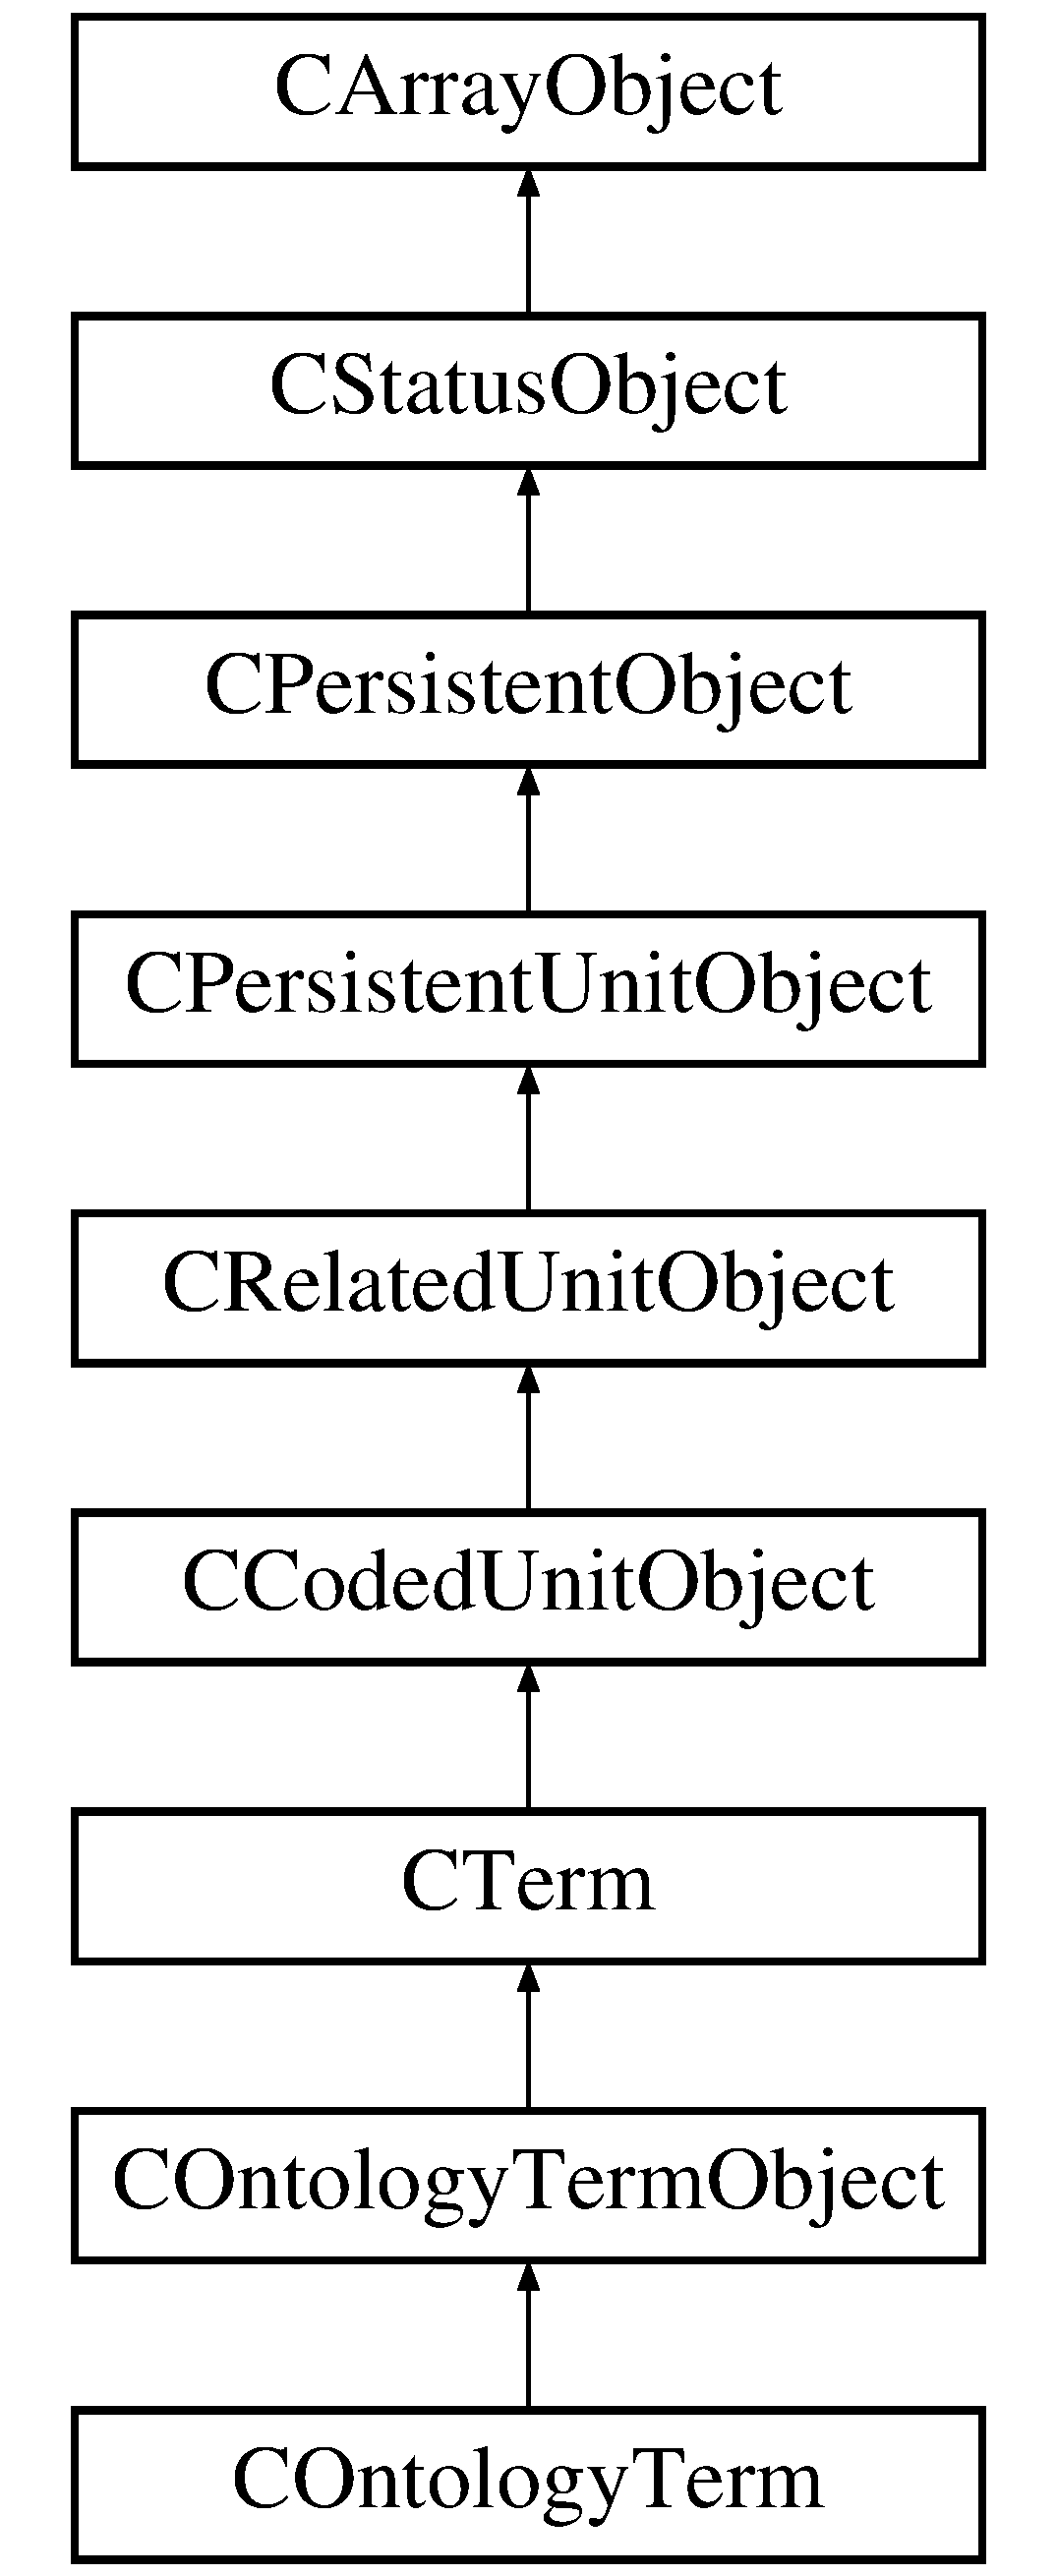
\includegraphics[height=9.000000cm]{class_c_term}
\end{center}
\end{figure}
\subsection*{Public Member Functions}
\begin{DoxyCompactItemize}
\item 
\hyperlink{class_c_term_a59a271c34a9f579bcf3177b392b6e31a}{N\-S} (\$the\-Value=N\-U\-L\-L, \$get\-Old=F\-A\-L\-S\-E)
\item 
\hyperlink{class_c_term_a67e5776ea8799b3e68d2ed9ca6dcde58}{Name} (\$the\-Value=N\-U\-L\-L, \$the\-Language=N\-U\-L\-L, \$get\-Old=F\-A\-L\-S\-E)
\item 
\hyperlink{class_c_term_a8452d05aa9a6687b0d2040158c58ea53}{Definition} (\$the\-Value=N\-U\-L\-L, \$the\-Language=N\-U\-L\-L, \$get\-Old=F\-A\-L\-S\-E)
\item 
\hyperlink{class_c_term_ac4193d704a54fbf35950151a36785103}{Description} (\$the\-Value=N\-U\-L\-L, \$the\-Language=N\-U\-L\-L, \$get\-Old=F\-A\-L\-S\-E)
\item 
\hyperlink{class_c_term_a2527808f249d6880b327e08a9cce0911}{Domain} (\$the\-Value=N\-U\-L\-L, \$the\-Operation=N\-U\-L\-L, \$get\-Old=F\-A\-L\-S\-E)
\item 
\hyperlink{class_c_term_a6ab25cb91c1a6de266e58ccad919ffba}{Category} (\$the\-Value=N\-U\-L\-L, \$the\-Operation=N\-U\-L\-L, \$get\-Old=F\-A\-L\-S\-E)
\item 
\hyperlink{class_c_term_adcaa8d79afde98b3d8bb76fbc894903f}{Synonym} (\$the\-Value, \$the\-Type, \$the\-Operation=N\-U\-L\-L, \$get\-Old=F\-A\-L\-S\-E)
\item 
\hyperlink{class_c_term_a0bbae7d5db15ba2b8aa94a17b441e366}{Xref} (\$the\-Value, \$the\-Type, \$the\-Operation=N\-U\-L\-L, \$get\-Old=F\-A\-L\-S\-E)
\item 
\hyperlink{class_c_term_abbbe3ae5901bbe1f83a2a2fe8e68df99}{Image} (\$the\-Kind, \$the\-Type, \$the\-Data=N\-U\-L\-L, \$get\-Old=F\-A\-L\-S\-E)
\item 
\hyperlink{class_c_term_af22cc12b6c41be83911b4cc4c5e54f94}{Namespace\-Name} (\$the\-Value=N\-U\-L\-L, \$get\-Old=F\-A\-L\-S\-E)
\item 
\hyperlink{class_c_term_a29c198c2f3c14c619d31b834639ad2fd}{Source} (\$the\-Value=N\-U\-L\-L, \$the\-Type=N\-U\-L\-L, \$get\-Old=F\-A\-L\-S\-E)
\item 
\hyperlink{class_c_term_ac9ffbfd23d67c874c47ccbff036c916b}{Version} (\$the\-Value=N\-U\-L\-L, \$get\-Old=F\-A\-L\-S\-E)
\end{DoxyCompactItemize}
\subsection*{Protected Member Functions}
\begin{DoxyCompactItemize}
\item 
\hyperlink{class_c_term_a7524effdc0db8f5ca045f306e3b6b50e}{\-\_\-index} ()
\end{DoxyCompactItemize}


\subsection{Member Function Documentation}
\hypertarget{class_c_term_a7524effdc0db8f5ca045f306e3b6b50e}{\index{C\-Term@{C\-Term}!\-\_\-index@{\-\_\-index}}
\index{\-\_\-index@{\-\_\-index}!CTerm@{C\-Term}}
\subsubsection[{\-\_\-index}]{\setlength{\rightskip}{0pt plus 5cm}C\-Term\-::\-\_\-index (
\begin{DoxyParamCaption}
{}
\end{DoxyParamCaption}
)\hspace{0.3cm}{\ttfamily [protected]}}}\label{class_c_term_a7524effdc0db8f5ca045f306e3b6b50e}
Return the object's unique index.

In this class we use the term's \hyperlink{}{namespace} and \hyperlink{}{code} to build the object's unique \hyperlink{}{identifier}; if the \hyperlink{}{namespace} is missing, we use the \hyperlink{}{code}; if the \hyperlink{}{namespace} is present, we use it as a prefix with the \hyperlink{}{code}, separated by the \hyperlink{}{separator} token.

protected \begin{DoxyReturn}{Returns}
string 
\end{DoxyReturn}


Reimplemented from \hyperlink{class_c_coded_unit_object_a990c19b8bf98d2784da81e3a3121ce56}{C\-Coded\-Unit\-Object}.

\hypertarget{class_c_term_a6ab25cb91c1a6de266e58ccad919ffba}{\index{C\-Term@{C\-Term}!Category@{Category}}
\index{Category@{Category}!CTerm@{C\-Term}}
\subsubsection[{Category}]{\setlength{\rightskip}{0pt plus 5cm}C\-Term\-::\-Category (
\begin{DoxyParamCaption}
\item[{}]{\$the\-Value = {\ttfamily NULL}, }
\item[{}]{\$the\-Operation = {\ttfamily NULL}, }
\item[{}]{\$get\-Old = {\ttfamily FALSE}}
\end{DoxyParamCaption}
)}}\label{class_c_term_a6ab25cb91c1a6de266e58ccad919ffba}
Manage categories.

This method can be used to handle the object's \hyperlink{}{categories}, it uses the standard accessor \hyperlink{class_c_attribute_a7d2e35b120eaa55529f78253f77dab48}{method} to manage the list of categories.

Each element of this list should indicate a category to which the current object belongs to.

For a more thorough reference of how this method works, please consult the \hyperlink{class_c_attribute_a7d2e35b120eaa55529f78253f77dab48}{C\-Attribute\-::\-Manage\-Array\-Offset} method, in which the second parameter will be the constant \hyperlink{}{k\-T\-A\-G\-\_\-\-C\-A\-T\-E\-G\-O\-R\-Y}.


\begin{DoxyParams}[1]{Parameters}
mixed & {\em \$the\-Value} & Value or index. \\
\hline
mixed & {\em \$the\-Operation} & Operation. \\
\hline
boolean & {\em \$get\-Old} & T\-R\-U\-E get old value.\\
\hline
\end{DoxyParams}
public \begin{DoxyReturn}{Returns}
mixed
\end{DoxyReturn}
\hyperlink{class_c_attribute_a7d2e35b120eaa55529f78253f77dab48}{C\-Attribute\-::\-Manage\-Array\-Offset()}

\begin{DoxySeeAlso}{See also}
k\-T\-A\-G\-\_\-\-C\-A\-T\-E\-G\-O\-R\-Y 
\end{DoxySeeAlso}
\hypertarget{class_c_term_a8452d05aa9a6687b0d2040158c58ea53}{\index{C\-Term@{C\-Term}!Definition@{Definition}}
\index{Definition@{Definition}!CTerm@{C\-Term}}
\subsubsection[{Definition}]{\setlength{\rightskip}{0pt plus 5cm}C\-Term\-::\-Definition (
\begin{DoxyParamCaption}
\item[{}]{\$the\-Value = {\ttfamily NULL}, }
\item[{}]{\$the\-Language = {\ttfamily NULL}, }
\item[{}]{\$get\-Old = {\ttfamily FALSE}}
\end{DoxyParamCaption}
)}}\label{class_c_term_a8452d05aa9a6687b0d2040158c58ea53}
Manage term definition.

This method can be used to manage the term \hyperlink{}{definition}, it manages an array of structures with the following offsets\-:


\begin{DoxyItemize}
\item {\itshape \hyperlink{}{k\-T\-A\-G\-\_\-\-L\-A\-N\-G\-U\-A\-G\-E}}\-: The definition's language, this element represents the code of the language in which the next element is expressed in. 
\item {\itshape \hyperlink{}{k\-T\-A\-G\-\_\-\-D\-A\-T\-A}}\-: The term definition or description. 
\end{DoxyItemize}

The parameters to this method are\-:


\begin{DoxyItemize}
\item {\bfseries \$the\-Value}\-: The definition or operation\-: 
\begin{DoxyItemize}
\item {\itshape N\-U\-L\-L}\-: Return the current value selected by the second parameter. 
\item {\itshape F\-A\-L\-S\-E}\-: Delete the value selected by the second parameter. 
\item {\itshape other}\-: Set value selected by the second parameter. 
\end{DoxyItemize}
\item {\bfseries \$the\-Language}\-: The definition's language code\-: 
\begin{DoxyItemize}
\item {\itshape N\-U\-L\-L}\-: This value indicates that the definition has no language, in general, when adding elements, this case applies to default elements. 
\item {\itshape other}\-: All other types will be interpreted as the language code. 
\end{DoxyItemize}
\item {\bfseries \$get\-Old}\-: Determines what the method will return\-: 
\begin{DoxyItemize}
\item {\itshape T\-R\-U\-E}\-: Return the value {\itshape before} it was eventually modified. 
\item {\itshape F\-A\-L\-S\-E}\-: Return the value {\itshape after} it was eventually modified. 
\end{DoxyItemize}
\end{DoxyItemize}


\begin{DoxyParams}[1]{Parameters}
mixed & {\em \$the\-Value} & Term definition or operation. \\
\hline
mixed & {\em \$the\-Language} & Term definition language code. \\
\hline
boolean & {\em \$get\-Old} & T\-R\-U\-E get old value.\\
\hline
\end{DoxyParams}
public \begin{DoxyReturn}{Returns}
string
\end{DoxyReturn}
\hyperlink{class_c_attribute_af163f41d2a8e052c09afe094195ca007}{C\-Attribute\-::\-Manage\-Typed\-Offset()}

\begin{DoxySeeAlso}{See also}
k\-T\-A\-G\-\_\-\-D\-E\-F\-I\-N\-I\-T\-I\-O\-N k\-T\-A\-G\-\_\-\-L\-A\-N\-G\-U\-A\-G\-E 
\end{DoxySeeAlso}
\hypertarget{class_c_term_ac4193d704a54fbf35950151a36785103}{\index{C\-Term@{C\-Term}!Description@{Description}}
\index{Description@{Description}!CTerm@{C\-Term}}
\subsubsection[{Description}]{\setlength{\rightskip}{0pt plus 5cm}C\-Term\-::\-Description (
\begin{DoxyParamCaption}
\item[{}]{\$the\-Value = {\ttfamily NULL}, }
\item[{}]{\$the\-Language = {\ttfamily NULL}, }
\item[{}]{\$get\-Old = {\ttfamily FALSE}}
\end{DoxyParamCaption}
)}}\label{class_c_term_ac4193d704a54fbf35950151a36785103}
Manage term description.

This method can be used to manage the term \hyperlink{}{description}, it manages an array of structures with the following offsets\-:


\begin{DoxyItemize}
\item {\itshape \hyperlink{}{k\-T\-A\-G\-\_\-\-L\-A\-N\-G\-U\-A\-G\-E}}\-: The description's language, this element represents the code of the language in which the next element is expressed in. 
\item {\itshape \hyperlink{}{k\-T\-A\-G\-\_\-\-D\-A\-T\-A}}\-: The term description or comment. 
\end{DoxyItemize}

The parameters to this method are\-:


\begin{DoxyItemize}
\item {\bfseries \$the\-Value}\-: The description or operation\-: 
\begin{DoxyItemize}
\item {\itshape N\-U\-L\-L}\-: Return the current value selected by the second parameter. 
\item {\itshape F\-A\-L\-S\-E}\-: Delete the value selected by the second parameter. 
\item {\itshape other}\-: Set value selected by the second parameter. 
\end{DoxyItemize}
\item {\bfseries \$the\-Language}\-: The description's language code\-: 
\begin{DoxyItemize}
\item {\itshape N\-U\-L\-L}\-: This value indicates that the description has no language, in general, when adding elements, this case applies to default elements. 
\item {\itshape other}\-: All other types will be interpreted as the language code. 
\end{DoxyItemize}
\item {\bfseries \$get\-Old}\-: Determines what the method will return\-: 
\begin{DoxyItemize}
\item {\itshape T\-R\-U\-E}\-: Return the value {\itshape before} it was eventually modified. 
\item {\itshape F\-A\-L\-S\-E}\-: Return the value {\itshape after} it was eventually modified. 
\end{DoxyItemize}
\end{DoxyItemize}


\begin{DoxyParams}[1]{Parameters}
mixed & {\em \$the\-Value} & Term description or operation. \\
\hline
mixed & {\em \$the\-Language} & Term description language code. \\
\hline
boolean & {\em \$get\-Old} & T\-R\-U\-E get old value.\\
\hline
\end{DoxyParams}
public \begin{DoxyReturn}{Returns}
string
\end{DoxyReturn}
\hyperlink{class_c_attribute_af163f41d2a8e052c09afe094195ca007}{C\-Attribute\-::\-Manage\-Typed\-Offset()}

\begin{DoxySeeAlso}{See also}
k\-T\-A\-G\-\_\-\-D\-E\-S\-C\-R\-I\-P\-T\-I\-O\-N k\-T\-A\-G\-\_\-\-L\-A\-N\-G\-U\-A\-G\-E 
\end{DoxySeeAlso}
\hypertarget{class_c_term_a2527808f249d6880b327e08a9cce0911}{\index{C\-Term@{C\-Term}!Domain@{Domain}}
\index{Domain@{Domain}!CTerm@{C\-Term}}
\subsubsection[{Domain}]{\setlength{\rightskip}{0pt plus 5cm}C\-Term\-::\-Domain (
\begin{DoxyParamCaption}
\item[{}]{\$the\-Value = {\ttfamily NULL}, }
\item[{}]{\$the\-Operation = {\ttfamily NULL}, }
\item[{}]{\$get\-Old = {\ttfamily FALSE}}
\end{DoxyParamCaption}
)}}\label{class_c_term_a2527808f249d6880b327e08a9cce0911}
Manage domains.

This method can be used to handle the object's \hyperlink{}{domains}, it uses the standard accessor \hyperlink{class_c_attribute_a7d2e35b120eaa55529f78253f77dab48}{method} to manage the list of domains.

Each element of this list should indicate a domain to which the current object belongs to.

For a more thorough reference of how this method works, please consult the \hyperlink{class_c_attribute_a7d2e35b120eaa55529f78253f77dab48}{C\-Attribute\-::\-Manage\-Array\-Offset} method, in which the second parameter will be the constant \hyperlink{}{k\-T\-A\-G\-\_\-\-C\-A\-T\-E\-G\-O\-R\-Y}.


\begin{DoxyParams}[1]{Parameters}
mixed & {\em \$the\-Value} & Value or index. \\
\hline
mixed & {\em \$the\-Operation} & Operation. \\
\hline
boolean & {\em \$get\-Old} & T\-R\-U\-E get old value.\\
\hline
\end{DoxyParams}
public \begin{DoxyReturn}{Returns}
mixed
\end{DoxyReturn}
\hyperlink{class_c_attribute_a7d2e35b120eaa55529f78253f77dab48}{C\-Attribute\-::\-Manage\-Array\-Offset()}

\begin{DoxySeeAlso}{See also}
k\-T\-A\-G\-\_\-\-D\-O\-M\-A\-I\-N 
\end{DoxySeeAlso}
\hypertarget{class_c_term_abbbe3ae5901bbe1f83a2a2fe8e68df99}{\index{C\-Term@{C\-Term}!Image@{Image}}
\index{Image@{Image}!CTerm@{C\-Term}}
\subsubsection[{Image}]{\setlength{\rightskip}{0pt plus 5cm}C\-Term\-::\-Image (
\begin{DoxyParamCaption}
\item[{}]{\$the\-Kind, }
\item[{}]{\$the\-Type, }
\item[{}]{\$the\-Data = {\ttfamily NULL}, }
\item[{}]{\$get\-Old = {\ttfamily FALSE}}
\end{DoxyParamCaption}
)}}\label{class_c_term_abbbe3ae5901bbe1f83a2a2fe8e68df99}
Manage cross-\/references.

This method can be used to manage the term's list of \hyperlink{}{images}, this \hyperlink{}{offset} is represented by an array of items holding three elements\-:


\begin{DoxyItemize}
\item {\itshape \hyperlink{}{k\-T\-A\-G\-\_\-\-K\-I\-N\-D}}\-: This element represents the kind or qualifier of the image, the element is required. 
\item {\itshape \hyperlink{}{k\-T\-A\-G\-\_\-\-T\-Y\-P\-E}}\-: This element represents the data type of the image, this element is required. 
\item {\itshape \hyperlink{}{k\-T\-A\-G\-\_\-\-D\-A\-T\-A}}\-: This element represents the image data which should be expressed in the data type declared in the \hyperlink{}{k\-T\-A\-G\-\_\-\-T\-Y\-P\-E} element. 
\end{DoxyItemize}

The method expects the following parameters\-:


\begin{DoxyItemize}
\item {\bfseries \$the\-Offset}\-: The main offset to manage. 
\item {\bfseries \$the\-Kind}\-: The item \hyperlink{}{kind}; it should be able to cast this value to a string which represents an index. 
\item {\bfseries \$the\-Type}\-: The item \hyperlink{}{type}; it should be able to cast this value to a string which represents an index. 
\item {\bfseries \$the\-Data}\-: This parameter represents the item's \hyperlink{}{data} element, or the operation to be performed\-: 
\begin{DoxyItemize}
\item {\itshape N\-U\-L\-L}\-: This indicates that we want to retrieve the data of the item with index matching the previous parameters. 
\item {\itshape F\-A\-L\-S\-E}\-: This indicates that we want to remove the item matching the index provided in the previous parameters. 
\item {\itshape other}\-: Any other value indicates that we want to add or replace the \hyperlink{}{data} element of the item matching the previous parameters. 
\end{DoxyItemize}
\item {\bfseries \$get\-Old}\-: Determines what the method will return\-: 
\begin{DoxyItemize}
\item {\itshape T\-R\-U\-E}\-: Return the element or list {\itshape before} it was eventually modified. 
\item {\itshape F\-A\-L\-S\-E}\-: Return the element or list {\itshape after} it was eventually modified. 
\end{DoxyItemize}
\end{DoxyItemize}

The method makes use of a static \hyperlink{class_c_attribute_ab0b7e532b3e0b4dca8fbab9b522e5332}{method}, please consult its reference for more information.


\begin{DoxyParams}[1]{Parameters}
mixed & {\em \$the\-Kind} & Image kind. \\
\hline
mixed & {\em \$the\-Type} & Image type. \\
\hline
mixed & {\em \$the\-Data} & Image value. \\
\hline
boolean & {\em \$get\-Old} & T\-R\-U\-E get old value.\\
\hline
\end{DoxyParams}
public \begin{DoxyReturn}{Returns}
string 
\end{DoxyReturn}
\hypertarget{class_c_term_a67e5776ea8799b3e68d2ed9ca6dcde58}{\index{C\-Term@{C\-Term}!Name@{Name}}
\index{Name@{Name}!CTerm@{C\-Term}}
\subsubsection[{Name}]{\setlength{\rightskip}{0pt plus 5cm}C\-Term\-::\-Name (
\begin{DoxyParamCaption}
\item[{}]{\$the\-Value = {\ttfamily NULL}, }
\item[{}]{\$the\-Language = {\ttfamily NULL}, }
\item[{}]{\$get\-Old = {\ttfamily FALSE}}
\end{DoxyParamCaption}
)}}\label{class_c_term_a67e5776ea8799b3e68d2ed9ca6dcde58}
Manage term name.

This method can be used to manage the term \hyperlink{}{name}, it manages an array of structures with the following offsets\-:


\begin{DoxyItemize}
\item {\itshape \hyperlink{}{k\-T\-A\-G\-\_\-\-L\-A\-N\-G\-U\-A\-G\-E}}\-: The name's language, this element represents the code of the language in which the next element is expressed in. 
\item {\itshape \hyperlink{}{k\-T\-A\-G\-\_\-\-D\-A\-T\-A}}\-: The term name or label. 
\end{DoxyItemize}

The parameters to this method are\-:


\begin{DoxyItemize}
\item {\bfseries \$the\-Value}\-: The name or operation\-: 
\begin{DoxyItemize}
\item {\itshape N\-U\-L\-L}\-: Return the current value selected by the second parameter. 
\item {\itshape F\-A\-L\-S\-E}\-: Delete the value selected by the second parameter. 
\item {\itshape other}\-: Set value selected by the second parameter. 
\end{DoxyItemize}
\item {\bfseries \$the\-Language}\-: The name's language code\-: 
\begin{DoxyItemize}
\item {\itshape N\-U\-L\-L}\-: This value indicates that the name has no language, in general, when adding elements, this case applies to default elements. 
\item {\itshape other}\-: All other types will be interpreted as the language code. 
\end{DoxyItemize}
\item {\bfseries \$get\-Old}\-: Determines what the method will return\-: 
\begin{DoxyItemize}
\item {\itshape T\-R\-U\-E}\-: Return the value {\itshape before} it was eventually modified. 
\item {\itshape F\-A\-L\-S\-E}\-: Return the value {\itshape after} it was eventually modified. 
\end{DoxyItemize}
\end{DoxyItemize}


\begin{DoxyParams}[1]{Parameters}
mixed & {\em \$the\-Value} & Term name or operation. \\
\hline
mixed & {\em \$the\-Language} & Term name language code. \\
\hline
boolean & {\em \$get\-Old} & T\-R\-U\-E get old value.\\
\hline
\end{DoxyParams}
public \begin{DoxyReturn}{Returns}
string
\end{DoxyReturn}
\hyperlink{class_c_attribute_af163f41d2a8e052c09afe094195ca007}{C\-Attribute\-::\-Manage\-Typed\-Offset()}

\begin{DoxySeeAlso}{See also}
k\-T\-A\-G\-\_\-\-N\-A\-M\-E k\-T\-A\-G\-\_\-\-L\-A\-N\-G\-U\-A\-G\-E 
\end{DoxySeeAlso}
\hypertarget{class_c_term_af22cc12b6c41be83911b4cc4c5e54f94}{\index{C\-Term@{C\-Term}!Namespace\-Name@{Namespace\-Name}}
\index{Namespace\-Name@{Namespace\-Name}!CTerm@{C\-Term}}
\subsubsection[{Namespace\-Name}]{\setlength{\rightskip}{0pt plus 5cm}C\-Term\-::\-Namespace\-Name (
\begin{DoxyParamCaption}
\item[{}]{\$the\-Value = {\ttfamily NULL}, }
\item[{}]{\$get\-Old = {\ttfamily FALSE}}
\end{DoxyParamCaption}
)}}\label{class_c_term_af22cc12b6c41be83911b4cc4c5e54f94}
Manage term namespace name.

This method can be used to handle the term \hyperlink{}{namespace}, it uses the standard accessor \hyperlink{class_c_attribute_a9d231a47718719fcd6c33f3d0ac91675}{method} to manage the \hyperlink{}{offset}.

This property represents the term's namespace name or acronym; not to be confused with the \hyperlink{}{k\-T\-A\-G\-\_\-\-N\-A\-M\-E\-S\-P\-A\-C\-E} offset which represents the namespace term reference.

For a more in-\/depth reference of this method, please consult the \hyperlink{class_c_attribute_a9d231a47718719fcd6c33f3d0ac91675}{C\-Attribute\-::\-Manage\-Offset} method, in which the second parameter will be the constant \hyperlink{}{k\-O\-F\-F\-S\-E\-T\-\_\-\-N\-A\-M\-E\-S\-P\-A\-C\-E}.


\begin{DoxyParams}[1]{Parameters}
mixed & {\em \$the\-Value} & Value. \\
\hline
boolean & {\em \$get\-Old} & T\-R\-U\-E get old value.\\
\hline
\end{DoxyParams}
public \begin{DoxyReturn}{Returns}
string
\end{DoxyReturn}
\hyperlink{class_c_attribute_a9d231a47718719fcd6c33f3d0ac91675}{C\-Attribute\-::\-Manage\-Offset()}

\begin{DoxySeeAlso}{See also}
k\-O\-F\-F\-S\-E\-T\-\_\-\-N\-A\-M\-E\-S\-P\-A\-C\-E 
\end{DoxySeeAlso}
\hypertarget{class_c_term_a59a271c34a9f579bcf3177b392b6e31a}{\index{C\-Term@{C\-Term}!N\-S@{N\-S}}
\index{N\-S@{N\-S}!CTerm@{C\-Term}}
\subsubsection[{N\-S}]{\setlength{\rightskip}{0pt plus 5cm}C\-Term\-::\-N\-S (
\begin{DoxyParamCaption}
\item[{}]{\$the\-Value = {\ttfamily NULL}, }
\item[{}]{\$get\-Old = {\ttfamily FALSE}}
\end{DoxyParamCaption}
)}}\label{class_c_term_a59a271c34a9f579bcf3177b392b6e31a}
Manage term namespace.

This method can be used to handle the term \hyperlink{}{namespace}, it uses the standard accessor \hyperlink{class_c_attribute_a9d231a47718719fcd6c33f3d0ac91675}{method} to manage the \hyperlink{}{offset}.

The namespace collects a series of terms under a common group in which each term \hyperlink{class_c_coded_unit_object_a56af949800e65f9a283239d2e455259f}{code} is unique, this \hyperlink{}{offset} represents a term reference.

For a more in-\/depth reference of this method, please consult the \hyperlink{class_c_attribute_a9d231a47718719fcd6c33f3d0ac91675}{C\-Attribute\-::\-Manage\-Offset} method, in which the second parameter will be the constant \hyperlink{}{k\-T\-A\-G\-\_\-\-N\-A\-M\-E\-S\-P\-A\-C\-E}.


\begin{DoxyParams}[1]{Parameters}
mixed & {\em \$the\-Value} & Value. \\
\hline
boolean & {\em \$get\-Old} & T\-R\-U\-E get old value.\\
\hline
\end{DoxyParams}
public \begin{DoxyReturn}{Returns}
string
\end{DoxyReturn}
\hyperlink{class_c_attribute_a9d231a47718719fcd6c33f3d0ac91675}{C\-Attribute\-::\-Manage\-Offset()}

\begin{DoxySeeAlso}{See also}
k\-T\-A\-G\-\_\-\-N\-A\-M\-E\-S\-P\-A\-C\-E 
\end{DoxySeeAlso}


Reimplemented in \hyperlink{class_c_ontology_term_object_a109414a9abe98e3997be238addfda6cf}{C\-Ontology\-Term\-Object}.

\hypertarget{class_c_term_a29c198c2f3c14c619d31b834639ad2fd}{\index{C\-Term@{C\-Term}!Source@{Source}}
\index{Source@{Source}!CTerm@{C\-Term}}
\subsubsection[{Source}]{\setlength{\rightskip}{0pt plus 5cm}C\-Term\-::\-Source (
\begin{DoxyParamCaption}
\item[{}]{\$the\-Value = {\ttfamily NULL}, }
\item[{}]{\$the\-Type = {\ttfamily NULL}, }
\item[{}]{\$get\-Old = {\ttfamily FALSE}}
\end{DoxyParamCaption}
)}}\label{class_c_term_a29c198c2f3c14c619d31b834639ad2fd}
Manage term sources.

This method can be used to manage the term \hyperlink{}{sources}, it manages an array of strings with the following offsets\-:


\begin{DoxyItemize}
\item {\itshape \hyperlink{}{k\-T\-A\-G\-\_\-\-K\-I\-N\-D}}\-: The source kind, this string can be used to define the type of the source, this element represents the array key, although technically it is implemented as an element to allow searching on all values. 
\item {\itshape \hyperlink{}{k\-T\-A\-G\-\_\-\-D\-A\-T\-A}}\-: The source, this element should hold the actual source reference, which should be convertable to a string. 
\end{DoxyItemize}

The parameters to this method are\-:


\begin{DoxyItemize}
\item {\bfseries \$the\-Value}\-: The value or operation\-: 
\begin{DoxyItemize}
\item {\itshape N\-U\-L\-L}\-: Return the current value selected by the second parameter. 
\item {\itshape F\-A\-L\-S\-E}\-: Delete the value selected by the second parameter. 
\item {\itshape other}\-: Set value selected by the second parameter. 
\end{DoxyItemize}
\item {\bfseries \$the\-Type}\-: The element type, kind or index\-: 
\begin{DoxyItemize}
\item {\itshape N\-U\-L\-L}\-: This value indicates that the phone has no type or kind, in general, when adding elements, this case applies to default elements. 
\item {\itshape other}\-: All other types will be interpreted as the kind or type of the phone number. 
\end{DoxyItemize}
\item {\bfseries \$get\-Old}\-: Determines what the method will return\-: 
\begin{DoxyItemize}
\item {\itshape T\-R\-U\-E}\-: Return the value {\itshape before} it was eventually modified. 
\item {\itshape F\-A\-L\-S\-E}\-: Return the value {\itshape after} it was eventually modified. 
\end{DoxyItemize}
\end{DoxyItemize}


\begin{DoxyParams}[1]{Parameters}
string & {\em \$the\-Value} & Source. \\
\hline
mixed & {\em \$the\-Type} & Source kind or index. \\
\hline
boolean & {\em \$get\-Old} & T\-R\-U\-E get old value.\\
\hline
\end{DoxyParams}
public \begin{DoxyReturn}{Returns}
string 
\end{DoxyReturn}
\hypertarget{class_c_term_adcaa8d79afde98b3d8bb76fbc894903f}{\index{C\-Term@{C\-Term}!Synonym@{Synonym}}
\index{Synonym@{Synonym}!CTerm@{C\-Term}}
\subsubsection[{Synonym}]{\setlength{\rightskip}{0pt plus 5cm}C\-Term\-::\-Synonym (
\begin{DoxyParamCaption}
\item[{}]{\$the\-Value, }
\item[{}]{\$the\-Type, }
\item[{}]{\$the\-Operation = {\ttfamily NULL}, }
\item[{}]{\$get\-Old = {\ttfamily FALSE}}
\end{DoxyParamCaption}
)}}\label{class_c_term_adcaa8d79afde98b3d8bb76fbc894903f}
Manage synonyms.

This method can be used to manage the term \hyperlink{}{synonyms} list, these elements are strings that can be considered synonyms of the current term.

This property is organised as an array of items structured as follows\-:


\begin{DoxyItemize}
\item {\itshape \hyperlink{}{k\-T\-A\-G\-\_\-\-K\-I\-N\-D}}\-: The synonym kind, its value is provided in the {\itshape \$the\-Type} parameter. 
\item {\itshape \hyperlink{}{k\-T\-A\-G\-\_\-\-D\-A\-T\-A}}\-: The synonym values organised as an array of strings. 
\end{DoxyItemize}

The method expects the following parameters\-:


\begin{DoxyItemize}
\item {\bfseries \$the\-Value}\-: The synonym value. 
\item {\bfseries \$the\-Type}\-: The synonym type. 
\item {\bfseries \$the\-Operation}\-: The operation\-: 
\begin{DoxyItemize}
\item {\itshape N\-U\-L\-L}\-: Return the current value selected by the previous parameters. 
\item {\itshape F\-A\-L\-S\-E}\-: Delete the value selected by the previous parameters. 
\item {\itshape other}\-: Set value selected by the previous parameters. 
\end{DoxyItemize}
\item {\bfseries \$get\-Old}\-: Determines what the method will return\-: 
\begin{DoxyItemize}
\item {\itshape T\-R\-U\-E}\-: Return the value {\itshape before} it was eventually modified. 
\item {\itshape F\-A\-L\-S\-E}\-: Return the value {\itshape after} it was eventually modified. 
\end{DoxyItemize}
\end{DoxyItemize}

The method makes use of a static \hyperlink{class_c_attribute_a9841820c02fde7e8f0b9c0a31b8ab1fa}{method}, please consult its reference for more information.


\begin{DoxyParams}[1]{Parameters}
string & {\em \$the\-Value} & Synonym. \\
\hline
mixed & {\em \$the\-Type} & Synonym type. \\
\hline
mixed & {\em \$the\-Operation} & Operation. \\
\hline
boolean & {\em \$get\-Old} & T\-R\-U\-E get old value.\\
\hline
\end{DoxyParams}
public \begin{DoxyReturn}{Returns}
string 
\end{DoxyReturn}


Reimplemented in \hyperlink{class_c_ontology_term_object_a96f637a86e1823dc61b2135a00ddfe26}{C\-Ontology\-Term\-Object}.

\hypertarget{class_c_term_ac9ffbfd23d67c874c47ccbff036c916b}{\index{C\-Term@{C\-Term}!Version@{Version}}
\index{Version@{Version}!CTerm@{C\-Term}}
\subsubsection[{Version}]{\setlength{\rightskip}{0pt plus 5cm}C\-Term\-::\-Version (
\begin{DoxyParamCaption}
\item[{}]{\$the\-Value = {\ttfamily NULL}, }
\item[{}]{\$get\-Old = {\ttfamily FALSE}}
\end{DoxyParamCaption}
)}}\label{class_c_term_ac9ffbfd23d67c874c47ccbff036c916b}
Manage version.

This method can be used to manage the term public \hyperlink{}{version}, it uses the standard accessor \hyperlink{class_c_attribute_a9d231a47718719fcd6c33f3d0ac91675}{method} to manage the \hyperlink{}{offset}\-:


\begin{DoxyItemize}
\item {\bfseries \$the\-Value}\-: The value or operation\-: 
\begin{DoxyItemize}
\item {\itshape N\-U\-L\-L}\-: Return the current value. 
\item {\itshape F\-A\-L\-S\-E}\-: Delete the value. 
\item {\itshape other}\-: Set value. 
\end{DoxyItemize}
\item {\bfseries \$get\-Old}\-: Determines what the method will return\-: 
\begin{DoxyItemize}
\item {\itshape T\-R\-U\-E}\-: Return the value {\itshape before} it was eventually modified. 
\item {\itshape F\-A\-L\-S\-E}\-: Return the value {\itshape after} it was eventually modified. 
\end{DoxyItemize}
\end{DoxyItemize}

Note that the object features another version \hyperlink{}{offset} which is automatically managed by the \hyperlink{class_c_persistent_unit_object}{ancestor}, the latter is an internal value, this one can be considere the {\itshape public} version.


\begin{DoxyParams}[1]{Parameters}
N\-U\-L\-L | F\-A\-L\-S\-E | string & {\em \$the\-Value} & Version or operation. \\
\hline
boolean & {\em \$get\-Old} & T\-R\-U\-E get old value.\\
\hline
\end{DoxyParams}
public \begin{DoxyReturn}{Returns}
string
\end{DoxyReturn}
\begin{DoxySeeAlso}{See also}
k\-O\-F\-F\-S\-E\-T\-\_\-\-V\-E\-R\-S\-I\-O\-N 
\end{DoxySeeAlso}
\hypertarget{class_c_term_a0bbae7d5db15ba2b8aa94a17b441e366}{\index{C\-Term@{C\-Term}!Xref@{Xref}}
\index{Xref@{Xref}!CTerm@{C\-Term}}
\subsubsection[{Xref}]{\setlength{\rightskip}{0pt plus 5cm}C\-Term\-::\-Xref (
\begin{DoxyParamCaption}
\item[{}]{\$the\-Value, }
\item[{}]{\$the\-Type, }
\item[{}]{\$the\-Operation = {\ttfamily NULL}, }
\item[{}]{\$get\-Old = {\ttfamily FALSE}}
\end{DoxyParamCaption}
)}}\label{class_c_term_a0bbae7d5db15ba2b8aa94a17b441e366}
Manage cross-\/references.

This method can be used to manage the term \hyperlink{}{cross-\/references} list, these elements are references to other terms that can be considered synonyms of the current term, the reference should be the term's \hyperlink{class_c_persistent_unit_object_ad1ca0920cf0df3c24351402f9afbf34b}{identifier}.

This property is organised as an array of items structured as follows\-:


\begin{DoxyItemize}
\item {\itshape \hyperlink{}{k\-T\-A\-G\-\_\-\-K\-I\-N\-D}}\-: The cross-\/reference kind, its value is provided in the {\itshape \$the\-Type} parameter. 
\item {\itshape \hyperlink{}{k\-T\-A\-G\-\_\-\-D\-A\-T\-A}}\-: The cross-\/reference values organised as an array of term identifiers. 
\end{DoxyItemize}

The method expects the following parameters\-:


\begin{DoxyItemize}
\item {\bfseries \$the\-Value}\-: The cross-\/reference. 
\item {\bfseries \$the\-Type}\-: The cross-\/reference type. 
\item {\bfseries \$the\-Operation}\-: The operation\-: 
\begin{DoxyItemize}
\item {\itshape N\-U\-L\-L}\-: Return the current value selected by the previous parameters. 
\item {\itshape F\-A\-L\-S\-E}\-: Delete the value selected by the previous parameters. 
\item {\itshape other}\-: Set value selected by the previous parameters. 
\end{DoxyItemize}
\item {\bfseries \$get\-Old}\-: Determines what the method will return\-: 
\begin{DoxyItemize}
\item {\itshape T\-R\-U\-E}\-: Return the value {\itshape before} it was eventually modified. 
\item {\itshape F\-A\-L\-S\-E}\-: Return the value {\itshape after} it was eventually modified. 
\end{DoxyItemize}
\end{DoxyItemize}

The method makes use of a static \hyperlink{class_c_attribute_a9841820c02fde7e8f0b9c0a31b8ab1fa}{method}, please consult its reference for more information.


\begin{DoxyParams}[1]{Parameters}
string & {\em \$the\-Value} & Object or operation. \\
\hline
mixed & {\em \$the\-Type} & Cross-\/reference type. \\
\hline
boolean & {\em \$get\-Old} & T\-R\-U\-E get old value.\\
\hline
\end{DoxyParams}
public \begin{DoxyReturn}{Returns}
string 
\end{DoxyReturn}


Reimplemented in \hyperlink{class_c_ontology_term_object_a32bb224840f965d3c2680895b52847c4}{C\-Ontology\-Term\-Object}.



The documentation for this class was generated from the following file\-:\begin{DoxyCompactItemize}
\item 
/\-Library/\-Web\-Server/\-Library/wrapper/classes/C\-Term.\-php\end{DoxyCompactItemize}

\hypertarget{class_c_user}{\section{C\-User Class Reference}
\label{class_c_user}\index{C\-User@{C\-User}}
}
Inheritance diagram for C\-User\-:\begin{figure}[H]
\begin{center}
\leavevmode
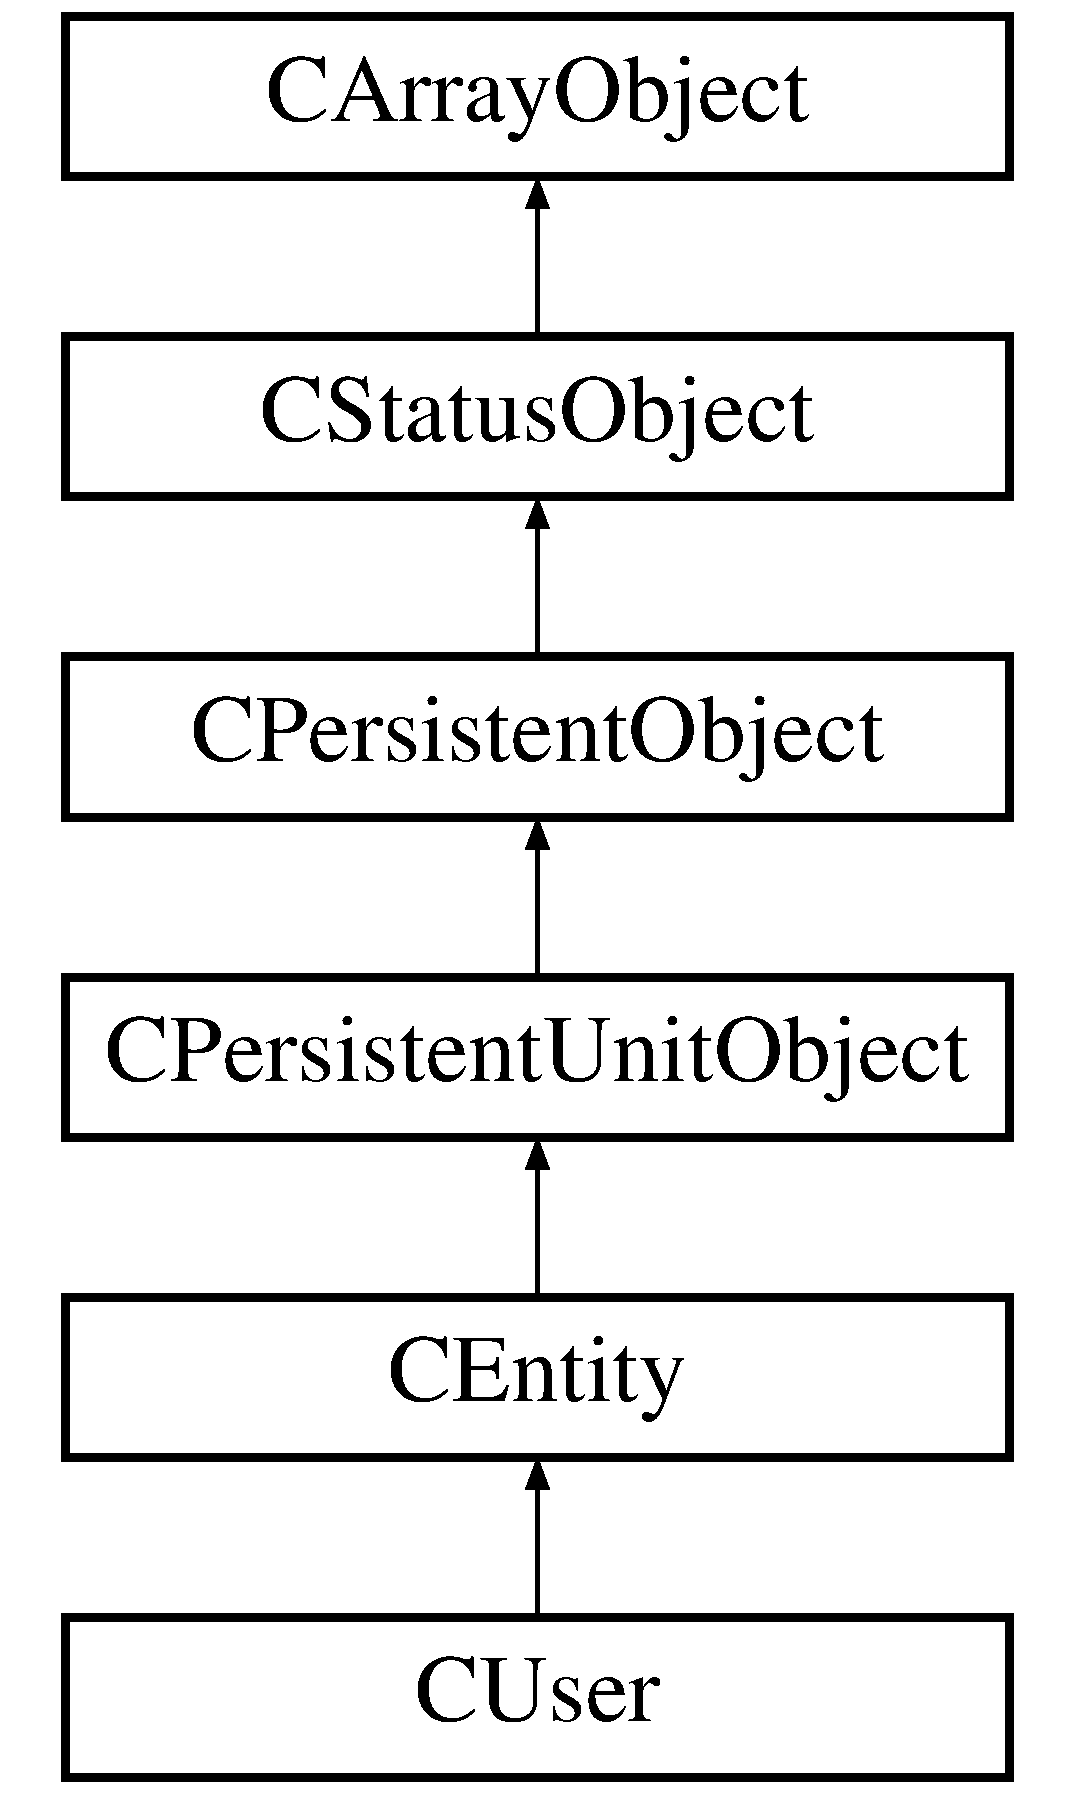
\includegraphics[height=8.000000cm]{class_c_user}
\end{center}
\end{figure}
\subsection*{Public Member Functions}
\begin{DoxyCompactItemize}
\item 
\hyperlink{class_c_user_af83ffccb40893a43d90eafe396cbdec1}{\-\_\-\-\_\-construct} (\$the\-Container=N\-U\-L\-L, \$the\-Identifier=N\-U\-L\-L, \$the\-Modifiers=k\-F\-L\-A\-G\-\_\-\-D\-E\-F\-A\-U\-L\-T)
\item 
\hyperlink{class_c_user_a0e6f1cf51ad23f971ed0999f8d248c8d}{Password} (\$the\-Value=N\-U\-L\-L, \$get\-Old=F\-A\-L\-S\-E)
\item 
\hyperlink{class_c_user_aace3446b9cacfe28cc1937c608fcc999}{offset\-Set} (\$the\-Offset, \$the\-Value)
\item 
\hyperlink{class_c_user_aed8557e18a89d868cedf5a48328b33b2}{offset\-Unset} (\$the\-Offset)
\end{DoxyCompactItemize}
\subsection*{Static Public Member Functions}
\begin{DoxyCompactItemize}
\item 
static \hyperlink{class_c_user_ada20d1f74260a4a5f67453bc9b4f3990}{Hash\-Index} (\$the\-Value)
\end{DoxyCompactItemize}
\subsection*{Protected Member Functions}
\begin{DoxyCompactItemize}
\item 
\hyperlink{class_c_user_aacdc43c5a38cb6b013ee9ce686b186e9}{\-\_\-\-Prepare\-Commit} (\&\$the\-Container, \&\$the\-Identifier, \&\$the\-Modifiers)
\end{DoxyCompactItemize}


\subsection{Constructor \& Destructor Documentation}
\hypertarget{class_c_user_af83ffccb40893a43d90eafe396cbdec1}{\index{C\-User@{C\-User}!\-\_\-\-\_\-construct@{\-\_\-\-\_\-construct}}
\index{\-\_\-\-\_\-construct@{\-\_\-\-\_\-construct}!CUser@{C\-User}}
\subsubsection[{\-\_\-\-\_\-construct}]{\setlength{\rightskip}{0pt plus 5cm}C\-User\-::\-\_\-\-\_\-construct (
\begin{DoxyParamCaption}
\item[{}]{\$the\-Container = {\ttfamily NULL}, }
\item[{}]{\$the\-Identifier = {\ttfamily NULL}, }
\item[{}]{\$the\-Modifiers = {\ttfamily kFLAG\-\_\-DEFAULT}}
\end{DoxyParamCaption}
)}}\label{class_c_user_af83ffccb40893a43d90eafe396cbdec1}
Instantiate class.

We \hyperlink{class_c_coded_unit_object_a314fc62af62314f5ac5acca2ac809900}{overload} the constructor to initialise the \hyperlink{class_c_status_object_a8429102e4f52f7558649b64f4e673a69}{inited} \hyperlink{}{flag} if the \hyperlink{class_c_user_a0e6f1cf51ad23f971ed0999f8d248c8d}{password} element is set.

We also pass the \hyperlink{class_c_persistent_object_aa8dc7db66e2af3d28c2035161a2aabf9}{encoded} \hyperlink{}{flag} to the parent constructor.


\begin{DoxyParams}[1]{Parameters}
mixed & {\em \$the\-Container} & Persistent container. \\
\hline
mixed & {\em \$the\-Identifier} & Object identifier. \\
\hline
bitfield & {\em \$the\-Modifiers} & Create modifiers.\\
\hline
\end{DoxyParams}
public 

Reimplemented from \hyperlink{class_c_coded_unit_object_a314fc62af62314f5ac5acca2ac809900}{C\-Coded\-Unit\-Object}.



\subsection{Member Function Documentation}
\hypertarget{class_c_user_aacdc43c5a38cb6b013ee9ce686b186e9}{\index{C\-User@{C\-User}!\-\_\-\-Prepare\-Commit@{\-\_\-\-Prepare\-Commit}}
\index{\-\_\-\-Prepare\-Commit@{\-\_\-\-Prepare\-Commit}!CUser@{C\-User}}
\subsubsection[{\-\_\-\-Prepare\-Commit}]{\setlength{\rightskip}{0pt plus 5cm}C\-User\-::\-\_\-\-Prepare\-Commit (
\begin{DoxyParamCaption}
\item[{\&}]{\$the\-Container, }
\item[{\&}]{\$the\-Identifier, }
\item[{\&}]{\$the\-Modifiers}
\end{DoxyParamCaption}
)\hspace{0.3cm}{\ttfamily [protected]}}}\label{class_c_user_aacdc43c5a38cb6b013ee9ce686b186e9}
Normalise parameters of a store.

We overload this method to add the \hyperlink{}{k\-E\-N\-T\-I\-T\-Y\-\_\-\-U\-S\-E\-R} \hyperlink{}{type} to the object prior \hyperlink{class_c_persistent_object_a88b1f2b11d3d60e0b3d33d8b0649b68a}{saving} it and we initialise the user \hyperlink{class_c_coded_unit_object_a56af949800e65f9a283239d2e455259f}{code}, if empty, with the \hyperlink{class_c_entity_acf65b6fb2f4195f6c649b4ca506c7899}{e-\/mail}.


\begin{DoxyParams}[1]{Parameters}
reference & {\em \&\$the\-Container} & Object container. \\
\hline
reference & {\em \&\$the\-Identifier} & Object identifier. \\
\hline
reference & {\em \&\$the\-Modifiers} & Commit modifiers.\\
\hline
\end{DoxyParams}
protected


\begin{DoxyExceptions}{Exceptions}
{\em \{@link} & \hyperlink{class_c_exception}{C\-Exception} \hyperlink{class_c_exception}{C\-Exception}\}\\
\hline
\end{DoxyExceptions}
\begin{DoxySeeAlso}{See also}
k\-E\-R\-R\-O\-R\-\_\-\-O\-P\-T\-I\-O\-N\-\_\-\-M\-I\-S\-S\-I\-N\-G 
\end{DoxySeeAlso}


Reimplemented from \hyperlink{class_c_entity_ac306808f0f8404fa405674cbe14fd441}{C\-Entity}.

\hypertarget{class_c_user_ada20d1f74260a4a5f67453bc9b4f3990}{\index{C\-User@{C\-User}!Hash\-Index@{Hash\-Index}}
\index{Hash\-Index@{Hash\-Index}!CUser@{C\-User}}
\subsubsection[{Hash\-Index}]{\setlength{\rightskip}{0pt plus 5cm}static C\-User\-::\-Hash\-Index (
\begin{DoxyParamCaption}
\item[{}]{\$the\-Value}
\end{DoxyParamCaption}
)\hspace{0.3cm}{\ttfamily [static]}}}\label{class_c_user_ada20d1f74260a4a5f67453bc9b4f3990}
Hash index.

This method can be used to format an identifier provided as a string, it will be used by the \hyperlink{class_c_persistent_unit_object_ad1ca0920cf0df3c24351402f9afbf34b}{\-\_\-id} method to format the result of the \hyperlink{class_c_coded_unit_object_a990c19b8bf98d2784da81e3a3121ce56}{\-\_\-index} method. One can consider this as the index hashing method for all derived classes.

In this class we take the provided \hyperlink{class_c_coded_unit_object_a56af949800e65f9a283239d2e455259f}{code} and prefix it with the \hyperlink{}{k\-E\-N\-T\-I\-T\-Y\-\_\-\-U\-S\-E\-R} token, the result will be \hyperlink{class_c_data_type_binary}{hashed}.


\begin{DoxyParams}[1]{Parameters}
string & {\em \$the\-Value} & Value to hash.\\
\hline
\end{DoxyParams}
\begin{DoxyReturn}{Returns}
string 
\end{DoxyReturn}


Reimplemented from \hyperlink{class_c_persistent_unit_object_af0e75c386b883074c8bb677bac500bb3}{C\-Persistent\-Unit\-Object}.

\hypertarget{class_c_user_aace3446b9cacfe28cc1937c608fcc999}{\index{C\-User@{C\-User}!offset\-Set@{offset\-Set}}
\index{offset\-Set@{offset\-Set}!CUser@{C\-User}}
\subsubsection[{offset\-Set}]{\setlength{\rightskip}{0pt plus 5cm}C\-User\-::offset\-Set (
\begin{DoxyParamCaption}
\item[{}]{\$the\-Offset, }
\item[{}]{\$the\-Value}
\end{DoxyParamCaption}
)}}\label{class_c_user_aace3446b9cacfe28cc1937c608fcc999}
Set a value for a given offset.

We overload this method to manage the \hyperlink{class_c_status_object_a8429102e4f52f7558649b64f4e673a69}{inited} \hyperlink{}{status}\-: this is set if the \hyperlink{}{name}, \hyperlink{}{e-\/mail}, \hyperlink{}{password} and the parent \hyperlink{}{code} are set.


\begin{DoxyParams}[1]{Parameters}
string & {\em \$the\-Offset} & Offset. \\
\hline
string | N\-U\-L\-L & {\em \$the\-Value} & Value to set at offset.\\
\hline
\end{DoxyParams}
public

\hyperlink{class_c_status_object_a8429102e4f52f7558649b64f4e673a69}{\-\_\-\-Is\-Inited()}  \hyperlink{class_c_persistent_object_a6520a7bcecf3f39fd61ec6d08f736e77}{\-\_\-\-Is\-Committed()} 

Reimplemented from \hyperlink{class_c_coded_unit_object_a49bb8f2956cb0551ba827b222778f295}{C\-Coded\-Unit\-Object}.

\hypertarget{class_c_user_aed8557e18a89d868cedf5a48328b33b2}{\index{C\-User@{C\-User}!offset\-Unset@{offset\-Unset}}
\index{offset\-Unset@{offset\-Unset}!CUser@{C\-User}}
\subsubsection[{offset\-Unset}]{\setlength{\rightskip}{0pt plus 5cm}C\-User\-::offset\-Unset (
\begin{DoxyParamCaption}
\item[{}]{\$the\-Offset}
\end{DoxyParamCaption}
)}}\label{class_c_user_aed8557e18a89d868cedf5a48328b33b2}
Reset a value for a given offset.

We overload this method to manage the \hyperlink{class_c_status_object_a8429102e4f52f7558649b64f4e673a69}{inited} \hyperlink{}{status}\-: this is set if the \hyperlink{}{name}, \hyperlink{}{e-\/mail}, \hyperlink{}{password} and the parent \hyperlink{}{code} are set.


\begin{DoxyParams}[1]{Parameters}
string & {\em \$the\-Offset} & Offset.\\
\hline
\end{DoxyParams}
public

\hyperlink{class_c_status_object_a8429102e4f52f7558649b64f4e673a69}{\-\_\-\-Is\-Inited()}  \hyperlink{class_c_persistent_object_a6520a7bcecf3f39fd61ec6d08f736e77}{\-\_\-\-Is\-Committed()} 

Reimplemented from \hyperlink{class_c_coded_unit_object_a5072e0f72c19260df212a4cf93c9f1cb}{C\-Coded\-Unit\-Object}.

\hypertarget{class_c_user_a0e6f1cf51ad23f971ed0999f8d248c8d}{\index{C\-User@{C\-User}!Password@{Password}}
\index{Password@{Password}!CUser@{C\-User}}
\subsubsection[{Password}]{\setlength{\rightskip}{0pt plus 5cm}C\-User\-::\-Password (
\begin{DoxyParamCaption}
\item[{}]{\$the\-Value = {\ttfamily NULL}, }
\item[{}]{\$get\-Old = {\ttfamily FALSE}}
\end{DoxyParamCaption}
)}}\label{class_c_user_a0e6f1cf51ad23f971ed0999f8d248c8d}
Manage user password.

This method can be used to manage the user \hyperlink{}{password}, it uses the standard accessor \hyperlink{class_c_attribute_a9d231a47718719fcd6c33f3d0ac91675}{method} to manage the \hyperlink{}{offset}\-:


\begin{DoxyItemize}
\item {\bfseries \$the\-Value}\-: The value or operation\-: 
\begin{DoxyItemize}
\item {\itshape N\-U\-L\-L}\-: Return the current value. 
\item {\itshape F\-A\-L\-S\-E}\-: Delete the value. 
\item {\itshape other}\-: Set value. 
\end{DoxyItemize}
\item {\bfseries \$get\-Old}\-: Determines what the method will return\-: 
\begin{DoxyItemize}
\item {\itshape T\-R\-U\-E}\-: Return the value {\itshape before} it was eventually modified. 
\item {\itshape F\-A\-L\-S\-E}\-: Return the value {\itshape after} it was eventually modified. 
\end{DoxyItemize}
\end{DoxyItemize}


\begin{DoxyParams}[1]{Parameters}
N\-U\-L\-L | F\-A\-L\-S\-E | string & {\em \$the\-Value} & User password or operation. \\
\hline
boolean & {\em \$get\-Old} & T\-R\-U\-E get old value.\\
\hline
\end{DoxyParams}
public \begin{DoxyReturn}{Returns}
string 
\end{DoxyReturn}


The documentation for this class was generated from the following file\-:\begin{DoxyCompactItemize}
\item 
/\-Library/\-Web\-Server/\-Library/wrapper/classes/C\-User.\-php\end{DoxyCompactItemize}

\hypertarget{class_c_warehouse_wrapper}{\section{C\-Warehouse\-Wrapper Class Reference}
\label{class_c_warehouse_wrapper}\index{C\-Warehouse\-Wrapper@{C\-Warehouse\-Wrapper}}
}
Inheritance diagram for C\-Warehouse\-Wrapper\-:\begin{figure}[H]
\begin{center}
\leavevmode
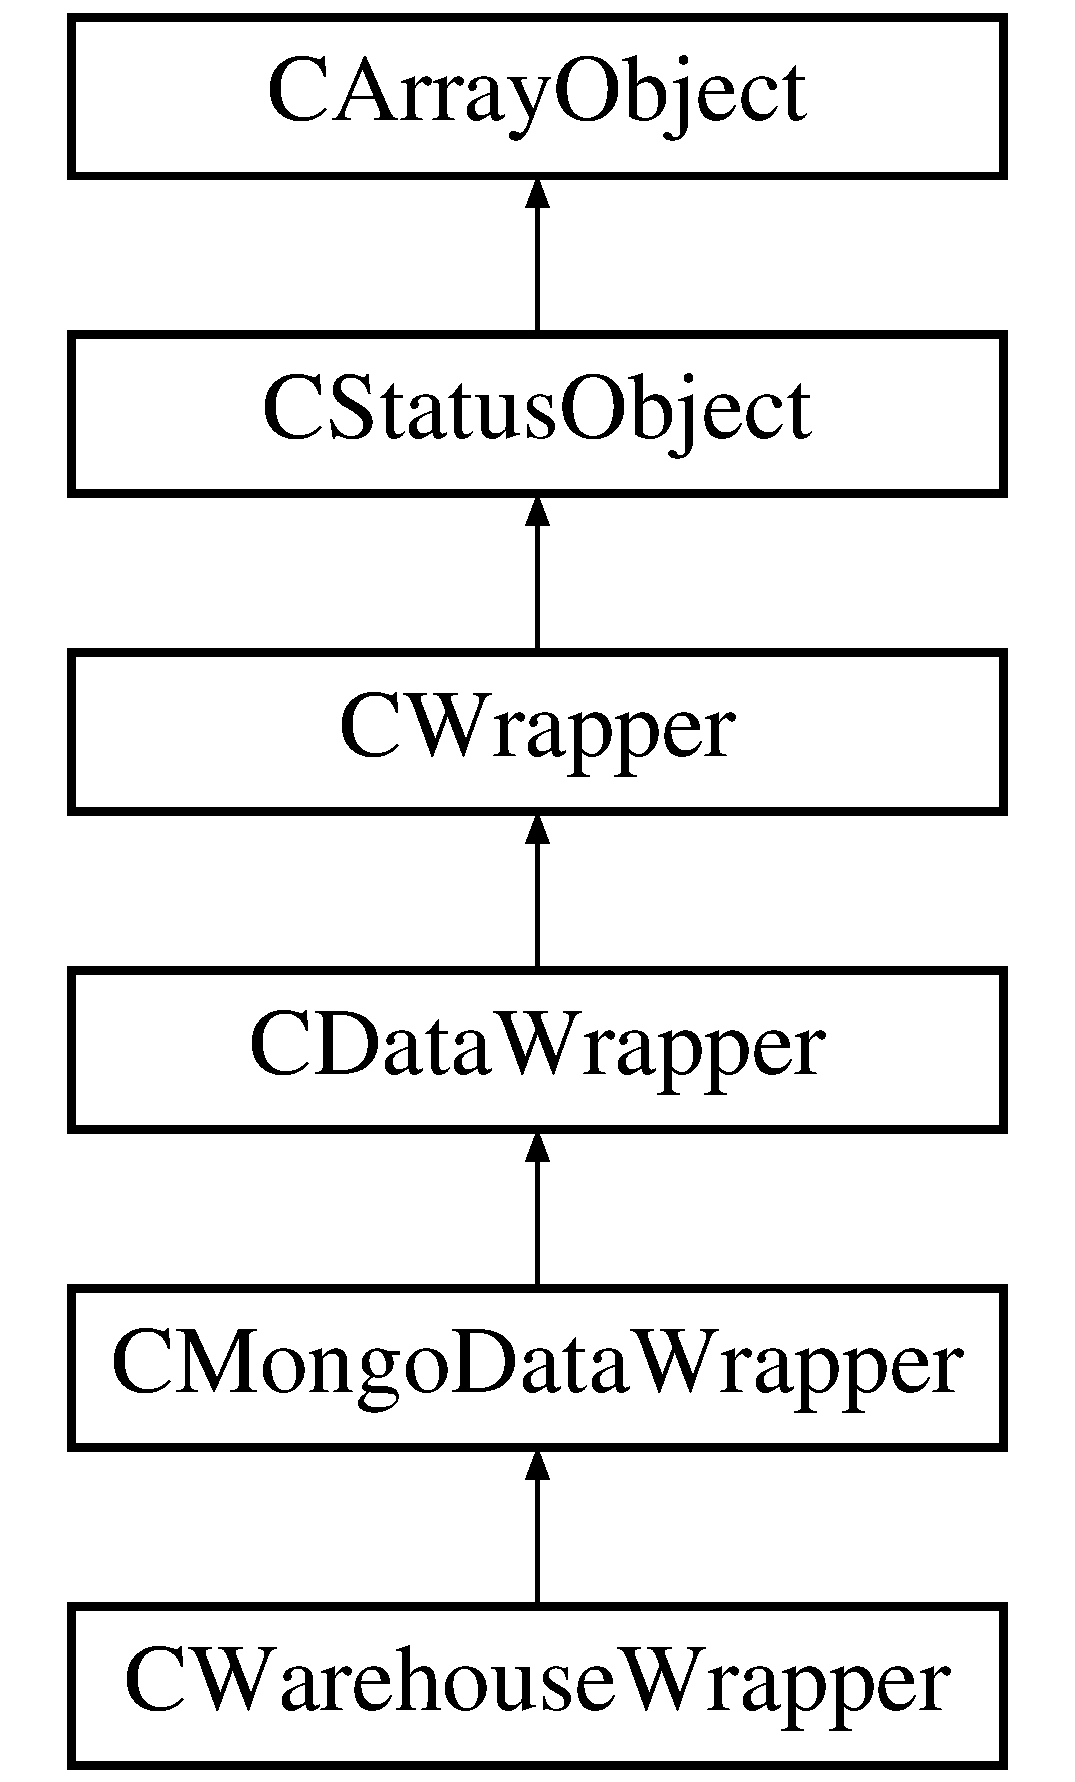
\includegraphics[height=6.000000cm]{class_c_warehouse_wrapper}
\end{center}
\end{figure}
\subsection*{Protected Member Functions}
\begin{DoxyCompactItemize}
\item 
\hyperlink{class_c_warehouse_wrapper_a8dd1de1d5595647b0999ffa6b658c605}{\-\_\-\-Init\-Options} ()
\item 
\hyperlink{class_c_warehouse_wrapper_ad1b028512dfbd4031ea443fd953bf178}{\-\_\-\-Init\-Resources} ()
\item 
\hyperlink{class_c_warehouse_wrapper_aab6f377ec08fc5f868a5ad65691964f6}{\-\_\-\-Parse\-Request} ()
\item 
\hyperlink{class_c_warehouse_wrapper_a4bd0282949f52ce148b60218c48ddde5}{\-\_\-\-Format\-Request} ()
\item 
\hyperlink{class_c_warehouse_wrapper_a1a4497011e288b0134b1d43b6029914b}{\-\_\-\-Parse\-Identifiers} ()
\item 
\hyperlink{class_c_warehouse_wrapper_a77a135708bb63dad7b6f43b93f38b655}{\-\_\-\-Parse\-Predicates} ()
\item 
\hyperlink{class_c_warehouse_wrapper_aea03fa2eb06da1201acbab5becfccdd2}{\-\_\-\-Parse\-Selectors} ()
\item 
\hyperlink{class_c_warehouse_wrapper_a675e18a0cae0a2050159b608c81e69b1}{\-\_\-\-Parse\-Direction} ()
\item 
\hyperlink{class_c_warehouse_wrapper_aeb1488dd1ab1e8494caff8f920b32ad7}{\-\_\-\-Parse\-User\-Code} ()
\item 
\hyperlink{class_c_warehouse_wrapper_a31f33bdb468cf377df7ac4c6d5496a95}{\-\_\-\-Parse\-User\-Pass} ()
\item 
\hyperlink{class_c_warehouse_wrapper_a687876da8f0dd0d0abb839b2b135ccbe}{\-\_\-\-Parse\-Levels} ()
\item 
\hyperlink{class_c_warehouse_wrapper_a728b298fc1f647792efb5bee38194a8a}{\-\_\-\-Format\-Identifiers} ()
\item 
\hyperlink{class_c_warehouse_wrapper_aa8f737fd107082e69ba1d82c228a9864}{\-\_\-\-Format\-Predicates} ()
\item 
\hyperlink{class_c_warehouse_wrapper_a948c44e335f8a89d50e09d430169533d}{\-\_\-\-Format\-Selectors} ()
\item 
\hyperlink{class_c_warehouse_wrapper_ab9506f24cc7dd6b001991f83bd2b5d55}{\-\_\-\-Validate\-Operation} ()
\item 
\hyperlink{class_c_warehouse_wrapper_a4b909b5b4aba967200ff72e3e6924b5e}{\-\_\-\-Handle\-Request} ()
\item 
\hyperlink{class_c_warehouse_wrapper_a1153f34202b1b0ddc32690c1c04c0bf7}{\-\_\-\-Handle\-\_\-\-Login} ()
\item 
\hyperlink{class_c_warehouse_wrapper_a547daf93a0bac707159ce50b6f429d7b}{\-\_\-\-Handle\-\_\-\-Get\-Nodes} ()
\item 
\hyperlink{class_c_warehouse_wrapper_a3c430fa7beda3d719cf75c21f4e1593d}{\-\_\-\-Handle\-\_\-\-Get\-Edges} ()
\item 
\hyperlink{class_c_warehouse_wrapper_acd8bbcad5d84122935a1a0f9868b2c5e}{\-\_\-\-Handle\-\_\-\-Query\-Ontologies} ()
\item 
\hyperlink{class_c_warehouse_wrapper_a9800cf5ca4bb22cd96a94ef542010adf}{\-\_\-\-Handle\-\_\-\-List\-Op} (\&\$the\-List)
\item 
\hyperlink{class_c_warehouse_wrapper_a6cd98a621a9cfc942cb192e1bd2ab392}{\-\_\-\-Escape\-Lucene} (\$the\-Element)
\item 
\hyperlink{class_c_warehouse_wrapper_a07ece9ec1b80bcba3acb40079e0a27d2}{\-\_\-\-Edge\-Parser} (\$the\-Edge, \&\$the\-Terms, \&\$the\-Nodes, \&\$the\-Edges)
\item 
\hyperlink{class_c_warehouse_wrapper_ab02604dd2c241b5fdf4e64c83914d6b5}{\-\_\-\-Traverse} (\&\$the\-List, \&\$the\-Terms, \&\$the\-Nodes, \&\$the\-Edges, \$the\-Level)
\end{DoxyCompactItemize}


\subsection{Member Function Documentation}
\hypertarget{class_c_warehouse_wrapper_a07ece9ec1b80bcba3acb40079e0a27d2}{\index{C\-Warehouse\-Wrapper@{C\-Warehouse\-Wrapper}!\-\_\-\-Edge\-Parser@{\-\_\-\-Edge\-Parser}}
\index{\-\_\-\-Edge\-Parser@{\-\_\-\-Edge\-Parser}!CWarehouseWrapper@{C\-Warehouse\-Wrapper}}
\subsubsection[{\-\_\-\-Edge\-Parser}]{\setlength{\rightskip}{0pt plus 5cm}C\-Warehouse\-Wrapper\-::\-\_\-\-Edge\-Parser (
\begin{DoxyParamCaption}
\item[{}]{\$the\-Edge, }
\item[{\&}]{\$the\-Terms, }
\item[{\&}]{\$the\-Nodes, }
\item[{\&}]{\$the\-Edges}
\end{DoxyParamCaption}
)\hspace{0.3cm}{\ttfamily [protected]}}}\label{class_c_warehouse_wrapper_a07ece9ec1b80bcba3acb40079e0a27d2}
Collect edge elements.

This method will collect the provided edge elements and set them into the provided parameters.

The parameters to this method are\-:


\begin{DoxyItemize}
\item {\bfseries \$the\-Edge}\-: Edge node to handle. 
\item {\bfseries \&\$the\-Terms}\-: Reference to the list of term identifiers. 
\item {\bfseries \&\$the\-Nodes}\-: Reference to the list of nodes. 
\item {\bfseries \&\$the\-Edges}\-: Reference to the list of edge elements. 
\end{DoxyItemize}

The method will return 1 if the edge was handled, 0 if not.


\begin{DoxyParams}[1]{Parameters}
Relationship & {\em \$the\-Edge} & Edge node to handle. \\
\hline
reference & {\em \&\$the\-Terms} & List of term identifiers. \\
\hline
reference & {\em \&\$the\-Nodes} & List of nodes. \\
\hline
reference & {\em \&\$the\-Edges} & List of edge references.\\
\hline
\end{DoxyParams}
protected \hypertarget{class_c_warehouse_wrapper_a6cd98a621a9cfc942cb192e1bd2ab392}{\index{C\-Warehouse\-Wrapper@{C\-Warehouse\-Wrapper}!\-\_\-\-Escape\-Lucene@{\-\_\-\-Escape\-Lucene}}
\index{\-\_\-\-Escape\-Lucene@{\-\_\-\-Escape\-Lucene}!CWarehouseWrapper@{C\-Warehouse\-Wrapper}}
\subsubsection[{\-\_\-\-Escape\-Lucene}]{\setlength{\rightskip}{0pt plus 5cm}C\-Warehouse\-Wrapper\-::\-\_\-\-Escape\-Lucene (
\begin{DoxyParamCaption}
\item[{}]{\$the\-Element}
\end{DoxyParamCaption}
)\hspace{0.3cm}{\ttfamily [protected]}}}\label{class_c_warehouse_wrapper_a6cd98a621a9cfc942cb192e1bd2ab392}
Escape Lucene element.

This method will escape the provided element to make it compatible with the Lucene query language, the method expects the provided parameter to be an element excluding specific lucene operators.


\begin{DoxyParams}[1]{Parameters}
string & {\em \$the\-Element} & Element to escape.\\
\hline
\end{DoxyParams}
protected \begin{DoxyReturn}{Returns}
string 
\end{DoxyReturn}
\hypertarget{class_c_warehouse_wrapper_a728b298fc1f647792efb5bee38194a8a}{\index{C\-Warehouse\-Wrapper@{C\-Warehouse\-Wrapper}!\-\_\-\-Format\-Identifiers@{\-\_\-\-Format\-Identifiers}}
\index{\-\_\-\-Format\-Identifiers@{\-\_\-\-Format\-Identifiers}!CWarehouseWrapper@{C\-Warehouse\-Wrapper}}
\subsubsection[{\-\_\-\-Format\-Identifiers}]{\setlength{\rightskip}{0pt plus 5cm}C\-Warehouse\-Wrapper\-::\-\_\-\-Format\-Identifiers (
\begin{DoxyParamCaption}
{}
\end{DoxyParamCaption}
)\hspace{0.3cm}{\ttfamily [protected]}}}\label{class_c_warehouse_wrapper_a728b298fc1f647792efb5bee38194a8a}
This method will format the request identifiers list.

In this class we handle the terms list \hyperlink{}{operation} by creating a query and using the \hyperlink{}{G\-E\-T} handler, in this method we create the \hyperlink{class_c_mongo_query}{query}.

protected

\hyperlink{class_c_data_wrapper_a30617297259d0ec38f793db4e1bb115d}{\-\_\-\-Decode\-Parameter()}

\begin{DoxySeeAlso}{See also}
k\-A\-P\-I\-\_\-\-O\-P\-T\-\_\-\-I\-D\-E\-N\-T\-I\-F\-I\-E\-R\-S 
\end{DoxySeeAlso}
\hypertarget{class_c_warehouse_wrapper_aa8f737fd107082e69ba1d82c228a9864}{\index{C\-Warehouse\-Wrapper@{C\-Warehouse\-Wrapper}!\-\_\-\-Format\-Predicates@{\-\_\-\-Format\-Predicates}}
\index{\-\_\-\-Format\-Predicates@{\-\_\-\-Format\-Predicates}!CWarehouseWrapper@{C\-Warehouse\-Wrapper}}
\subsubsection[{\-\_\-\-Format\-Predicates}]{\setlength{\rightskip}{0pt plus 5cm}C\-Warehouse\-Wrapper\-::\-\_\-\-Format\-Predicates (
\begin{DoxyParamCaption}
{}
\end{DoxyParamCaption}
)\hspace{0.3cm}{\ttfamily [protected]}}}\label{class_c_warehouse_wrapper_aa8f737fd107082e69ba1d82c228a9864}
This method will format the request predicates list.

In this class we \hyperlink{class_c_data_wrapper_a30617297259d0ec38f793db4e1bb115d}{decode} the parameter.

protected

\hyperlink{class_c_data_wrapper_a30617297259d0ec38f793db4e1bb115d}{\-\_\-\-Decode\-Parameter()}

\begin{DoxySeeAlso}{See also}
k\-A\-P\-I\-\_\-\-O\-P\-T\-\_\-\-P\-R\-E\-D\-I\-C\-A\-T\-E\-S 
\end{DoxySeeAlso}
\hypertarget{class_c_warehouse_wrapper_a4bd0282949f52ce148b60218c48ddde5}{\index{C\-Warehouse\-Wrapper@{C\-Warehouse\-Wrapper}!\-\_\-\-Format\-Request@{\-\_\-\-Format\-Request}}
\index{\-\_\-\-Format\-Request@{\-\_\-\-Format\-Request}!CWarehouseWrapper@{C\-Warehouse\-Wrapper}}
\subsubsection[{\-\_\-\-Format\-Request}]{\setlength{\rightskip}{0pt plus 5cm}C\-Warehouse\-Wrapper\-::\-\_\-\-Format\-Request (
\begin{DoxyParamCaption}
{}
\end{DoxyParamCaption}
)\hspace{0.3cm}{\ttfamily [protected]}}}\label{class_c_warehouse_wrapper_a4bd0282949f52ce148b60218c48ddde5}
Format request.

This method should perform any needed formatting before the request will be handled.

In this class we handle the parameters to be decoded

protected

\hyperlink{class_c_warehouse_wrapper_a728b298fc1f647792efb5bee38194a8a}{\-\_\-\-Format\-Identifiers()} 

Reimplemented from \hyperlink{class_c_mongo_data_wrapper_abbc0d41394dda4a27eefa8481065749a}{C\-Mongo\-Data\-Wrapper}.

\hypertarget{class_c_warehouse_wrapper_a948c44e335f8a89d50e09d430169533d}{\index{C\-Warehouse\-Wrapper@{C\-Warehouse\-Wrapper}!\-\_\-\-Format\-Selectors@{\-\_\-\-Format\-Selectors}}
\index{\-\_\-\-Format\-Selectors@{\-\_\-\-Format\-Selectors}!CWarehouseWrapper@{C\-Warehouse\-Wrapper}}
\subsubsection[{\-\_\-\-Format\-Selectors}]{\setlength{\rightskip}{0pt plus 5cm}C\-Warehouse\-Wrapper\-::\-\_\-\-Format\-Selectors (
\begin{DoxyParamCaption}
{}
\end{DoxyParamCaption}
)\hspace{0.3cm}{\ttfamily [protected]}}}\label{class_c_warehouse_wrapper_a948c44e335f8a89d50e09d430169533d}
This method will format the request selectors list.

This method will convert the attribute/value pairs provided in the \hyperlink{}{k\-A\-P\-I\-\_\-\-O\-P\-T\-\_\-\-A\-T\-T\-R\-I\-B\-U\-T\-E\-S} parameter into a Lucene compatible query, connecting all clauses in {\itshape A\-N\-D}.

Note that the method will enforce the \hyperlink{}{k\-A\-P\-I\-\_\-\-O\-P\-T\-\_\-\-A\-T\-T\-R\-I\-B\-U\-T\-E\-S} parameter by initialising it with the \hyperlink{}{root} \hyperlink{}{kind} selection.

protected

\hyperlink{class_c_data_wrapper_a30617297259d0ec38f793db4e1bb115d}{\-\_\-\-Decode\-Parameter()}

\begin{DoxySeeAlso}{See also}
k\-A\-P\-I\-\_\-\-O\-P\-T\-\_\-\-A\-T\-T\-R\-I\-B\-U\-T\-E\-S 
\end{DoxySeeAlso}
\hypertarget{class_c_warehouse_wrapper_a3c430fa7beda3d719cf75c21f4e1593d}{\index{C\-Warehouse\-Wrapper@{C\-Warehouse\-Wrapper}!\-\_\-\-Handle\-\_\-\-Get\-Edges@{\-\_\-\-Handle\-\_\-\-Get\-Edges}}
\index{\-\_\-\-Handle\-\_\-\-Get\-Edges@{\-\_\-\-Handle\-\_\-\-Get\-Edges}!CWarehouseWrapper@{C\-Warehouse\-Wrapper}}
\subsubsection[{\-\_\-\-Handle\-\_\-\-Get\-Edges}]{\setlength{\rightskip}{0pt plus 5cm}C\-Warehouse\-Wrapper\-::\-\_\-\-Handle\-\_\-\-Get\-Edges (
\begin{DoxyParamCaption}
{}
\end{DoxyParamCaption}
)\hspace{0.3cm}{\ttfamily [protected]}}}\label{class_c_warehouse_wrapper_a3c430fa7beda3d719cf75c21f4e1593d}
Handle \hyperlink{}{get-\/edges} request.

This method will return the following structure\-:


\begin{DoxyItemize}
\item {\itshape \hyperlink{}{k\-A\-P\-I\-\_\-\-R\-E\-S\-P\-O\-N\-S\-E\-\_\-\-T\-E\-R\-M\-S}}\-: The list of terms related to the list of subject and object nodes and the list of predicate terms as follows\-: 
\begin{DoxyItemize}
\item {\itshape Index}\-: The term \hyperlink{}{identifier}. 
\item {\itshape Value}\-: The term properties. 
\end{DoxyItemize}
\item {\itshape \hyperlink{}{k\-A\-P\-I\-\_\-\-R\-E\-S\-P\-O\-N\-S\-E\-\_\-\-N\-O\-D\-E\-S}}\-: The list of subject and object nodes as follows\-: 
\begin{DoxyItemize}
\item {\itshape Index}\-: The node I\-D. 
\item {\itshape Value}\-: The node properties. 
\end{DoxyItemize}
\item {\itshape \hyperlink{}{k\-A\-P\-I\-\_\-\-R\-E\-S\-P\-O\-N\-S\-E\-\_\-\-E\-D\-G\-E\-S}}\-: The list of edges as an array structured as follows\-: 
\begin{DoxyItemize}
\item {\itshape Index}\-: The edge identifier. 
\item {\itshape Value}\-: An array structured as follows\-: 
\begin{DoxyItemize}
\item {\itshape \hyperlink{}{k\-A\-P\-I\-\_\-\-R\-E\-S\-P\-O\-N\-S\-E\-\_\-\-S\-U\-B\-J\-E\-C\-T}}\-: The subject \hyperlink{class_c_ontology_node}{node} I\-D. 
\item {\itshape \hyperlink{}{k\-A\-P\-I\-\_\-\-R\-E\-S\-P\-O\-N\-S\-E\-\_\-\-P\-R\-E\-D\-I\-C\-A\-T\-E}}\-: The predicate \hyperlink{class_c_ontology_term}{term} \hyperlink{}{identifier}. 
\item {\itshape \hyperlink{}{k\-A\-P\-I\-\_\-\-R\-E\-S\-P\-O\-N\-S\-E\-\_\-\-O\-B\-J\-E\-C\-T}}\-: The object \hyperlink{class_c_ontology_node}{node} I\-D. 
\end{DoxyItemize}
\end{DoxyItemize}
\end{DoxyItemize}

The method will interpret the contents of the \hyperlink{}{k\-A\-P\-I\-\_\-\-O\-P\-T\-\_\-\-I\-D\-E\-N\-T\-I\-F\-I\-E\-R\-S} parameter depending on whether the \hyperlink{}{k\-A\-P\-I\-\_\-\-O\-P\-T\-\_\-\-D\-I\-R\-E\-C\-T\-I\-O\-N} parameter was provided or not\-:


\begin{DoxyItemize}
\item {\itshape \hyperlink{}{k\-A\-P\-I\-\_\-\-O\-P\-T\-\_\-\-D\-I\-R\-E\-C\-T\-I\-O\-N} not provided}\-: In this case the method will treat the \hyperlink{}{k\-A\-P\-I\-\_\-\-O\-P\-T\-\_\-\-I\-D\-E\-N\-T\-I\-F\-I\-E\-R\-S} parameter elements as a list of \hyperlink{class_c_ontology_edge}{edge} identifiers to be matched. 
\item {\itshape \hyperlink{}{k\-A\-P\-I\-\_\-\-O\-P\-T\-\_\-\-D\-I\-R\-E\-C\-T\-I\-O\-N} provided}\-: In this case the method will treat the \hyperlink{}{k\-A\-P\-I\-\_\-\-O\-P\-T\-\_\-\-I\-D\-E\-N\-T\-I\-F\-I\-E\-R\-S} parameter elements as a list of \hyperlink{class_c_ontology_node}{node} identifiers for which we want to retrieve connected \hyperlink{class_c_ontology_edge}{edges} in the direction provided in the \hyperlink{}{k\-A\-P\-I\-\_\-\-O\-P\-T\-\_\-\-D\-I\-R\-E\-C\-T\-I\-O\-N} parameter\-: 
\begin{DoxyItemize}
\item {\itshape \hyperlink{}{k\-A\-P\-I\-\_\-\-D\-I\-R\-E\-C\-T\-I\-O\-N\-\_\-\-I\-N}}\-: The service will return all \hyperlink{class_c_ontology_edge}{edges} that point to the \hyperlink{class_c_ontology_node}{nodes} provided in the \hyperlink{}{k\-A\-P\-I\-\_\-\-O\-P\-T\-\_\-\-I\-D\-E\-N\-T\-I\-F\-I\-E\-R\-S} parameter. 
\item {\itshape \hyperlink{}{k\-A\-P\-I\-\_\-\-D\-I\-R\-E\-C\-T\-I\-O\-N\-\_\-\-O\-U\-T}}\-: The service will return all \hyperlink{class_c_ontology_edge}{edges} pointing from the \hyperlink{class_c_ontology_node}{nodes} provided in the \hyperlink{}{k\-A\-P\-I\-\_\-\-O\-P\-T\-\_\-\-I\-D\-E\-N\-T\-I\-F\-I\-E\-R\-S} parameter. 
\item {\itshape \hyperlink{}{k\-A\-P\-I\-\_\-\-D\-I\-R\-E\-C\-T\-I\-O\-N\-\_\-\-A\-L\-L}}\-: The service will return all \hyperlink{class_c_ontology_edge}{edges} connected in any way to the \hyperlink{class_c_ontology_node}{nodes} provided in the \hyperlink{}{k\-A\-P\-I\-\_\-\-O\-P\-T\-\_\-\-I\-D\-E\-N\-T\-I\-F\-I\-E\-R\-S} parameter. 
\end{DoxyItemize}
\end{DoxyItemize}

If the \hyperlink{}{k\-A\-P\-I\-\_\-\-O\-P\-T\-\_\-\-P\-R\-E\-D\-I\-C\-A\-T\-E\-S} parameter was provided, only those \hyperlink{class_c_ontology_edge}{edges} whose type matches any of the predicate \hyperlink{class_c_ontology_term}{term} identifiers provided in that parameter will be selected.

If the \hyperlink{}{k\-A\-P\-I\-\_\-\-O\-P\-T\-\_\-\-I\-D\-E\-N\-T\-I\-F\-I\-E\-R\-S} parameter was not provided, the method will return the above structure with no content.

protected \hypertarget{class_c_warehouse_wrapper_a547daf93a0bac707159ce50b6f429d7b}{\index{C\-Warehouse\-Wrapper@{C\-Warehouse\-Wrapper}!\-\_\-\-Handle\-\_\-\-Get\-Nodes@{\-\_\-\-Handle\-\_\-\-Get\-Nodes}}
\index{\-\_\-\-Handle\-\_\-\-Get\-Nodes@{\-\_\-\-Handle\-\_\-\-Get\-Nodes}!CWarehouseWrapper@{C\-Warehouse\-Wrapper}}
\subsubsection[{\-\_\-\-Handle\-\_\-\-Get\-Nodes}]{\setlength{\rightskip}{0pt plus 5cm}C\-Warehouse\-Wrapper\-::\-\_\-\-Handle\-\_\-\-Get\-Nodes (
\begin{DoxyParamCaption}
{}
\end{DoxyParamCaption}
)\hspace{0.3cm}{\ttfamily [protected]}}}\label{class_c_warehouse_wrapper_a547daf93a0bac707159ce50b6f429d7b}
Handle \hyperlink{}{get-\/nodes} request.

This method expects the \hyperlink{}{k\-A\-P\-I\-\_\-\-O\-P\-T\-\_\-\-I\-D\-E\-N\-T\-I\-F\-I\-E\-R\-S} parameter to hold a list of node I\-Ds, the method will query these nodes and return the following structure\-:


\begin{DoxyItemize}
\item {\itshape \hyperlink{}{k\-A\-P\-I\-\_\-\-R\-E\-S\-P\-O\-N\-S\-E\-\_\-\-T\-E\-R\-M\-S}}\-: The list of terms related to the list of nodes as follows\-: 
\begin{DoxyItemize}
\item {\itshape Index}\-: The term \hyperlink{}{identifier}. 
\item {\itshape Value}\-: The term properties. 
\end{DoxyItemize}
\item {\itshape \hyperlink{}{k\-A\-P\-I\-\_\-\-R\-E\-S\-P\-O\-N\-S\-E\-\_\-\-N\-O\-D\-E\-S}}\-: The list of nodes as follows\-: 
\begin{DoxyItemize}
\item {\itshape Index}\-: The node I\-D. 
\item {\itshape Value}\-: The node properties. 
\end{DoxyItemize}
\end{DoxyItemize}

If the \hyperlink{}{k\-A\-P\-I\-\_\-\-O\-P\-T\-\_\-\-I\-D\-E\-N\-T\-I\-F\-I\-E\-R\-S} parameter was not provided, the method will return the above structure with no content.

protected \hypertarget{class_c_warehouse_wrapper_a9800cf5ca4bb22cd96a94ef542010adf}{\index{C\-Warehouse\-Wrapper@{C\-Warehouse\-Wrapper}!\-\_\-\-Handle\-\_\-\-List\-Op@{\-\_\-\-Handle\-\_\-\-List\-Op}}
\index{\-\_\-\-Handle\-\_\-\-List\-Op@{\-\_\-\-Handle\-\_\-\-List\-Op}!CWarehouseWrapper@{C\-Warehouse\-Wrapper}}
\subsubsection[{\-\_\-\-Handle\-\_\-\-List\-Op}]{\setlength{\rightskip}{0pt plus 5cm}C\-Warehouse\-Wrapper\-::\-\_\-\-Handle\-\_\-\-List\-Op (
\begin{DoxyParamCaption}
\item[{\&}]{\$the\-List}
\end{DoxyParamCaption}
)\hspace{0.3cm}{\ttfamily [protected]}}}\label{class_c_warehouse_wrapper_a9800cf5ca4bb22cd96a94ef542010adf}
Handle \hyperlink{}{list} operations request.

This method will handle the \hyperlink{}{k\-A\-P\-I\-\_\-\-O\-P\-\_\-\-H\-E\-L\-P} request, which should return the list of supported operations.


\begin{DoxyParams}[1]{Parameters}
reference & {\em \$the\-List} & Receives operations list.\\
\hline
\end{DoxyParams}
protected 

Reimplemented from \hyperlink{class_c_mongo_data_wrapper_a1ca51f95510a94bf26e004ef2e8e8d37}{C\-Mongo\-Data\-Wrapper}.

\hypertarget{class_c_warehouse_wrapper_a1153f34202b1b0ddc32690c1c04c0bf7}{\index{C\-Warehouse\-Wrapper@{C\-Warehouse\-Wrapper}!\-\_\-\-Handle\-\_\-\-Login@{\-\_\-\-Handle\-\_\-\-Login}}
\index{\-\_\-\-Handle\-\_\-\-Login@{\-\_\-\-Handle\-\_\-\-Login}!CWarehouseWrapper@{C\-Warehouse\-Wrapper}}
\subsubsection[{\-\_\-\-Handle\-\_\-\-Login}]{\setlength{\rightskip}{0pt plus 5cm}C\-Warehouse\-Wrapper\-::\-\_\-\-Handle\-\_\-\-Login (
\begin{DoxyParamCaption}
{}
\end{DoxyParamCaption}
)\hspace{0.3cm}{\ttfamily [protected]}}}\label{class_c_warehouse_wrapper_a1153f34202b1b0ddc32690c1c04c0bf7}
Handle \hyperlink{}{login} request.

This method will first \hyperlink{class_c_user_af83ffccb40893a43d90eafe396cbdec1}{load} the user by using its \hyperlink{class_c_coded_unit_object_a56af949800e65f9a283239d2e455259f}{code}, then match the \hyperlink{class_c_user_a0e6f1cf51ad23f971ed0999f8d248c8d}{password}; if they match it will return the user record.

protected \hypertarget{class_c_warehouse_wrapper_acd8bbcad5d84122935a1a0f9868b2c5e}{\index{C\-Warehouse\-Wrapper@{C\-Warehouse\-Wrapper}!\-\_\-\-Handle\-\_\-\-Query\-Ontologies@{\-\_\-\-Handle\-\_\-\-Query\-Ontologies}}
\index{\-\_\-\-Handle\-\_\-\-Query\-Ontologies@{\-\_\-\-Handle\-\_\-\-Query\-Ontologies}!CWarehouseWrapper@{C\-Warehouse\-Wrapper}}
\subsubsection[{\-\_\-\-Handle\-\_\-\-Query\-Ontologies}]{\setlength{\rightskip}{0pt plus 5cm}C\-Warehouse\-Wrapper\-::\-\_\-\-Handle\-\_\-\-Query\-Ontologies (
\begin{DoxyParamCaption}
{}
\end{DoxyParamCaption}
)\hspace{0.3cm}{\ttfamily [protected]}}}\label{class_c_warehouse_wrapper_acd8bbcad5d84122935a1a0f9868b2c5e}
Handle \hyperlink{}{query-\/nodes} request.

This method expects the \hyperlink{}{k\-A\-P\-I\-\_\-\-O\-P\-T\-\_\-\-A\-T\-T\-R\-I\-B\-U\-T\-E\-S} parameter to hold a list of key/value pairs filter that will be added to the default \hyperlink{}{root} \hyperlink{}{kind} query; if the parameter was omitted, the method will select all ontologies.

This method will return the following structure\-:


\begin{DoxyItemize}
\item {\itshape \hyperlink{}{k\-A\-P\-I\-\_\-\-R\-E\-S\-P\-O\-N\-S\-E\-\_\-\-T\-E\-R\-M\-S}}\-: The list of \hyperlink{class_c_ontology_term}{terms} related to the \hyperlink{class_c_graph_node_ad830025d2d6650006eb6e737bd4f32c0}{ontologies} as follows\-: 
\begin{DoxyItemize}
\item {\itshape Index}\-: The term \hyperlink{}{identifier}. 
\item {\itshape Value}\-: The term properties. 
\end{DoxyItemize}
\item {\itshape \hyperlink{}{k\-A\-P\-I\-\_\-\-R\-E\-S\-P\-O\-N\-S\-E\-\_\-\-N\-O\-D\-E\-S}}\-: The list of \hyperlink{class_c_graph_node_ad830025d2d6650006eb6e737bd4f32c0}{ontologies} as follows\-: 
\begin{DoxyItemize}
\item {\itshape Index}\-: The \hyperlink{class_c_graph_node_ad830025d2d6650006eb6e737bd4f32c0}{node} I\-D. 
\item {\itshape Value}\-: The \hyperlink{class_c_graph_node_ad830025d2d6650006eb6e737bd4f32c0}{node} properties. 
\end{DoxyItemize}
\end{DoxyItemize}

protected \hypertarget{class_c_warehouse_wrapper_a4b909b5b4aba967200ff72e3e6924b5e}{\index{C\-Warehouse\-Wrapper@{C\-Warehouse\-Wrapper}!\-\_\-\-Handle\-Request@{\-\_\-\-Handle\-Request}}
\index{\-\_\-\-Handle\-Request@{\-\_\-\-Handle\-Request}!CWarehouseWrapper@{C\-Warehouse\-Wrapper}}
\subsubsection[{\-\_\-\-Handle\-Request}]{\setlength{\rightskip}{0pt plus 5cm}C\-Warehouse\-Wrapper\-::\-\_\-\-Handle\-Request (
\begin{DoxyParamCaption}
{}
\end{DoxyParamCaption}
)\hspace{0.3cm}{\ttfamily [protected]}}}\label{class_c_warehouse_wrapper_a4b909b5b4aba967200ff72e3e6924b5e}
Handle request.

This method will handle the request.

protected 

Reimplemented from \hyperlink{class_c_mongo_data_wrapper_a811af7e7574a459bc56afa3afa99e1a8}{C\-Mongo\-Data\-Wrapper}.

\hypertarget{class_c_warehouse_wrapper_a8dd1de1d5595647b0999ffa6b658c605}{\index{C\-Warehouse\-Wrapper@{C\-Warehouse\-Wrapper}!\-\_\-\-Init\-Options@{\-\_\-\-Init\-Options}}
\index{\-\_\-\-Init\-Options@{\-\_\-\-Init\-Options}!CWarehouseWrapper@{C\-Warehouse\-Wrapper}}
\subsubsection[{\-\_\-\-Init\-Options}]{\setlength{\rightskip}{0pt plus 5cm}C\-Warehouse\-Wrapper\-::\-\_\-\-Init\-Options (
\begin{DoxyParamCaption}
{}
\end{DoxyParamCaption}
)\hspace{0.3cm}{\ttfamily [protected]}}}\label{class_c_warehouse_wrapper_a8dd1de1d5595647b0999ffa6b658c605}
Initialise options.

This method is responsible for parsing and setting all default and provided options, derived classes should overload this method to handle custom options.

In this class we enforce \hyperlink{}{paging} options if the \hyperlink{}{identifiers\} list was not provided and the operation is get  k\-A\-P\-I\-\_\-\-O\-P\-\_\-\-G\-E\-T\-\_\-\-T\-E\-R\-M\-S terms\}.   private   k\-A\-P\-I\-\_\-\-D\-A\-T\-A\-\_\-\-R\-E\-Q\-U\-E\-S\-T k\-A\-P\-I\-\_\-\-D\-A\-T\-A\-\_\-\-T\-I\-M\-I\-N\-G }

Reimplemented from \hyperlink{class_c_data_wrapper_a85c97add738d08f2f2a9958ffbda6c03}{C\-Data\-Wrapper}.

\hypertarget{class_c_warehouse_wrapper_ad1b028512dfbd4031ea443fd953bf178}{\index{C\-Warehouse\-Wrapper@{C\-Warehouse\-Wrapper}!\-\_\-\-Init\-Resources@{\-\_\-\-Init\-Resources}}
\index{\-\_\-\-Init\-Resources@{\-\_\-\-Init\-Resources}!CWarehouseWrapper@{C\-Warehouse\-Wrapper}}
\subsubsection[{\-\_\-\-Init\-Resources}]{\setlength{\rightskip}{0pt plus 5cm}C\-Warehouse\-Wrapper\-::\-\_\-\-Init\-Resources (
\begin{DoxyParamCaption}
{}
\end{DoxyParamCaption}
)\hspace{0.3cm}{\ttfamily [protected]}}}\label{class_c_warehouse_wrapper_ad1b028512dfbd4031ea443fd953bf178}
Initialise resources.

In this class we instantiate the Neo4j client.

protected 

Reimplemented from \hyperlink{class_c_mongo_data_wrapper_a33ff97c26b97d00a67f97d41f67ce47b}{C\-Mongo\-Data\-Wrapper}.

\hypertarget{class_c_warehouse_wrapper_a675e18a0cae0a2050159b608c81e69b1}{\index{C\-Warehouse\-Wrapper@{C\-Warehouse\-Wrapper}!\-\_\-\-Parse\-Direction@{\-\_\-\-Parse\-Direction}}
\index{\-\_\-\-Parse\-Direction@{\-\_\-\-Parse\-Direction}!CWarehouseWrapper@{C\-Warehouse\-Wrapper}}
\subsubsection[{\-\_\-\-Parse\-Direction}]{\setlength{\rightskip}{0pt plus 5cm}C\-Warehouse\-Wrapper\-::\-\_\-\-Parse\-Direction (
\begin{DoxyParamCaption}
{}
\end{DoxyParamCaption}
)\hspace{0.3cm}{\ttfamily [protected]}}}\label{class_c_warehouse_wrapper_a675e18a0cae0a2050159b608c81e69b1}
Parse direction.

This method will parse the relations \hyperlink{}{direction} parameter.

protected

\begin{DoxySeeAlso}{See also}
k\-A\-P\-I\-\_\-\-D\-A\-T\-A\-\_\-\-R\-E\-Q\-U\-E\-S\-T k\-A\-P\-I\-\_\-\-O\-P\-T\-\_\-\-D\-I\-R\-E\-C\-T\-I\-O\-N 
\end{DoxySeeAlso}
\hypertarget{class_c_warehouse_wrapper_a1a4497011e288b0134b1d43b6029914b}{\index{C\-Warehouse\-Wrapper@{C\-Warehouse\-Wrapper}!\-\_\-\-Parse\-Identifiers@{\-\_\-\-Parse\-Identifiers}}
\index{\-\_\-\-Parse\-Identifiers@{\-\_\-\-Parse\-Identifiers}!CWarehouseWrapper@{C\-Warehouse\-Wrapper}}
\subsubsection[{\-\_\-\-Parse\-Identifiers}]{\setlength{\rightskip}{0pt plus 5cm}C\-Warehouse\-Wrapper\-::\-\_\-\-Parse\-Identifiers (
\begin{DoxyParamCaption}
{}
\end{DoxyParamCaption}
)\hspace{0.3cm}{\ttfamily [protected]}}}\label{class_c_warehouse_wrapper_a1a4497011e288b0134b1d43b6029914b}
Parse identifiers.

This method will parse the user \hyperlink{}{identifiers} parameter.

protected

\begin{DoxySeeAlso}{See also}
k\-A\-P\-I\-\_\-\-D\-A\-T\-A\-\_\-\-R\-E\-Q\-U\-E\-S\-T k\-A\-P\-I\-\_\-\-O\-P\-T\-\_\-\-I\-D\-E\-N\-T\-I\-F\-I\-E\-R\-S 
\end{DoxySeeAlso}
\hypertarget{class_c_warehouse_wrapper_a687876da8f0dd0d0abb839b2b135ccbe}{\index{C\-Warehouse\-Wrapper@{C\-Warehouse\-Wrapper}!\-\_\-\-Parse\-Levels@{\-\_\-\-Parse\-Levels}}
\index{\-\_\-\-Parse\-Levels@{\-\_\-\-Parse\-Levels}!CWarehouseWrapper@{C\-Warehouse\-Wrapper}}
\subsubsection[{\-\_\-\-Parse\-Levels}]{\setlength{\rightskip}{0pt plus 5cm}C\-Warehouse\-Wrapper\-::\-\_\-\-Parse\-Levels (
\begin{DoxyParamCaption}
{}
\end{DoxyParamCaption}
)\hspace{0.3cm}{\ttfamily [protected]}}}\label{class_c_warehouse_wrapper_a687876da8f0dd0d0abb839b2b135ccbe}
Parse level.

This method will parse the relations \hyperlink{}{levels} parameter.

protected

\begin{DoxySeeAlso}{See also}
k\-A\-P\-I\-\_\-\-D\-A\-T\-A\-\_\-\-R\-E\-Q\-U\-E\-S\-T k\-A\-P\-I\-\_\-\-O\-P\-T\-\_\-\-L\-E\-V\-E\-L\-S 
\end{DoxySeeAlso}
\hypertarget{class_c_warehouse_wrapper_a77a135708bb63dad7b6f43b93f38b655}{\index{C\-Warehouse\-Wrapper@{C\-Warehouse\-Wrapper}!\-\_\-\-Parse\-Predicates@{\-\_\-\-Parse\-Predicates}}
\index{\-\_\-\-Parse\-Predicates@{\-\_\-\-Parse\-Predicates}!CWarehouseWrapper@{C\-Warehouse\-Wrapper}}
\subsubsection[{\-\_\-\-Parse\-Predicates}]{\setlength{\rightskip}{0pt plus 5cm}C\-Warehouse\-Wrapper\-::\-\_\-\-Parse\-Predicates (
\begin{DoxyParamCaption}
{}
\end{DoxyParamCaption}
)\hspace{0.3cm}{\ttfamily [protected]}}}\label{class_c_warehouse_wrapper_a77a135708bb63dad7b6f43b93f38b655}
Parse predicates.

This method will parse the user \hyperlink{}{predicates} parameter.

protected

\begin{DoxySeeAlso}{See also}
k\-A\-P\-I\-\_\-\-D\-A\-T\-A\-\_\-\-R\-E\-Q\-U\-E\-S\-T k\-A\-P\-I\-\_\-\-O\-P\-T\-\_\-\-P\-R\-E\-D\-I\-C\-A\-T\-E\-S 
\end{DoxySeeAlso}
\hypertarget{class_c_warehouse_wrapper_aab6f377ec08fc5f868a5ad65691964f6}{\index{C\-Warehouse\-Wrapper@{C\-Warehouse\-Wrapper}!\-\_\-\-Parse\-Request@{\-\_\-\-Parse\-Request}}
\index{\-\_\-\-Parse\-Request@{\-\_\-\-Parse\-Request}!CWarehouseWrapper@{C\-Warehouse\-Wrapper}}
\subsubsection[{\-\_\-\-Parse\-Request}]{\setlength{\rightskip}{0pt plus 5cm}C\-Warehouse\-Wrapper\-::\-\_\-\-Parse\-Request (
\begin{DoxyParamCaption}
{}
\end{DoxyParamCaption}
)\hspace{0.3cm}{\ttfamily [protected]}}}\label{class_c_warehouse_wrapper_aab6f377ec08fc5f868a5ad65691964f6}
Parse request.

We overload this method to parse the user \hyperlink{}{code} and \hyperlink{}{password} tags.

protected

\hyperlink{class_c_warehouse_wrapper_aeb1488dd1ab1e8494caff8f920b32ad7}{\-\_\-\-Parse\-User\-Code()}  \hyperlink{class_c_warehouse_wrapper_a31f33bdb468cf377df7ac4c6d5496a95}{\-\_\-\-Parse\-User\-Pass()} 

Reimplemented from \hyperlink{class_c_mongo_data_wrapper_a8ac2f23cfc78f3fba6b256718ed2d105}{C\-Mongo\-Data\-Wrapper}.

\hypertarget{class_c_warehouse_wrapper_aea03fa2eb06da1201acbab5becfccdd2}{\index{C\-Warehouse\-Wrapper@{C\-Warehouse\-Wrapper}!\-\_\-\-Parse\-Selectors@{\-\_\-\-Parse\-Selectors}}
\index{\-\_\-\-Parse\-Selectors@{\-\_\-\-Parse\-Selectors}!CWarehouseWrapper@{C\-Warehouse\-Wrapper}}
\subsubsection[{\-\_\-\-Parse\-Selectors}]{\setlength{\rightskip}{0pt plus 5cm}C\-Warehouse\-Wrapper\-::\-\_\-\-Parse\-Selectors (
\begin{DoxyParamCaption}
{}
\end{DoxyParamCaption}
)\hspace{0.3cm}{\ttfamily [protected]}}}\label{class_c_warehouse_wrapper_aea03fa2eb06da1201acbab5becfccdd2}
Parse identifiers.

This method will parse the attribute \hyperlink{}{selectors} parameter.

protected

\begin{DoxySeeAlso}{See also}
k\-A\-P\-I\-\_\-\-D\-A\-T\-A\-\_\-\-R\-E\-Q\-U\-E\-S\-T k\-A\-P\-I\-\_\-\-O\-P\-T\-\_\-\-A\-T\-T\-R\-I\-B\-U\-T\-E\-S 
\end{DoxySeeAlso}
\hypertarget{class_c_warehouse_wrapper_aeb1488dd1ab1e8494caff8f920b32ad7}{\index{C\-Warehouse\-Wrapper@{C\-Warehouse\-Wrapper}!\-\_\-\-Parse\-User\-Code@{\-\_\-\-Parse\-User\-Code}}
\index{\-\_\-\-Parse\-User\-Code@{\-\_\-\-Parse\-User\-Code}!CWarehouseWrapper@{C\-Warehouse\-Wrapper}}
\subsubsection[{\-\_\-\-Parse\-User\-Code}]{\setlength{\rightskip}{0pt plus 5cm}C\-Warehouse\-Wrapper\-::\-\_\-\-Parse\-User\-Code (
\begin{DoxyParamCaption}
{}
\end{DoxyParamCaption}
)\hspace{0.3cm}{\ttfamily [protected]}}}\label{class_c_warehouse_wrapper_aeb1488dd1ab1e8494caff8f920b32ad7}
Parse user code.

This method will parse the user \hyperlink{}{code} parameter.

protected

\begin{DoxySeeAlso}{See also}
k\-A\-P\-I\-\_\-\-D\-A\-T\-A\-\_\-\-R\-E\-Q\-U\-E\-S\-T k\-A\-P\-I\-\_\-\-O\-P\-T\-\_\-\-U\-S\-E\-R\-\_\-\-C\-O\-D\-E 
\end{DoxySeeAlso}
\hypertarget{class_c_warehouse_wrapper_a31f33bdb468cf377df7ac4c6d5496a95}{\index{C\-Warehouse\-Wrapper@{C\-Warehouse\-Wrapper}!\-\_\-\-Parse\-User\-Pass@{\-\_\-\-Parse\-User\-Pass}}
\index{\-\_\-\-Parse\-User\-Pass@{\-\_\-\-Parse\-User\-Pass}!CWarehouseWrapper@{C\-Warehouse\-Wrapper}}
\subsubsection[{\-\_\-\-Parse\-User\-Pass}]{\setlength{\rightskip}{0pt plus 5cm}C\-Warehouse\-Wrapper\-::\-\_\-\-Parse\-User\-Pass (
\begin{DoxyParamCaption}
{}
\end{DoxyParamCaption}
)\hspace{0.3cm}{\ttfamily [protected]}}}\label{class_c_warehouse_wrapper_a31f33bdb468cf377df7ac4c6d5496a95}
Parse user password.

This method will parse the user \hyperlink{}{password} parameter.

protected

\begin{DoxySeeAlso}{See also}
k\-A\-P\-I\-\_\-\-D\-A\-T\-A\-\_\-\-R\-E\-Q\-U\-E\-S\-T k\-A\-P\-I\-\_\-\-O\-P\-T\-\_\-\-U\-S\-E\-R\-\_\-\-P\-A\-S\-S 
\end{DoxySeeAlso}
\hypertarget{class_c_warehouse_wrapper_ab02604dd2c241b5fdf4e64c83914d6b5}{\index{C\-Warehouse\-Wrapper@{C\-Warehouse\-Wrapper}!\-\_\-\-Traverse@{\-\_\-\-Traverse}}
\index{\-\_\-\-Traverse@{\-\_\-\-Traverse}!CWarehouseWrapper@{C\-Warehouse\-Wrapper}}
\subsubsection[{\-\_\-\-Traverse}]{\setlength{\rightskip}{0pt plus 5cm}C\-Warehouse\-Wrapper\-::\-\_\-\-Traverse (
\begin{DoxyParamCaption}
\item[{\&}]{\$the\-List, }
\item[{\&}]{\$the\-Terms, }
\item[{\&}]{\$the\-Nodes, }
\item[{\&}]{\$the\-Edges, }
\item[{}]{\$the\-Level}
\end{DoxyParamCaption}
)\hspace{0.3cm}{\ttfamily [protected]}}}\label{class_c_warehouse_wrapper_ab02604dd2c241b5fdf4e64c83914d6b5}
Traverse graph.

This method will traverse the graph in the direction set in the \hyperlink{}{k\-A\-P\-I\-\_\-\-O\-P\-T\-\_\-\-D\-I\-R\-E\-C\-T\-I\-O\-N} parameter and \hyperlink{class_c_warehouse_wrapper_a07ece9ec1b80bcba3acb40079e0a27d2}{collect} all found edge elements in the provided parameters.

The parameters to this method are\-:


\begin{DoxyItemize}
\item {\bfseries \&\$the\-List}\-: List of current level node identifiers. 
\item {\bfseries \&\$the\-Terms}\-: Reference to the list of term identifiers. 
\item {\bfseries \&\$the\-Nodes}\-: Reference to the list of nodes. 
\item {\bfseries \&\$the\-Edges}\-: Reference to the list of edge elements. 
\item {\bfseries \$the\-Level}\-: Current traversal depth level, 0 means the lowest. 
\end{DoxyItemize}

The method will return the number of processed elements count.


\begin{DoxyParams}[1]{Parameters}
reference & {\em \&\$the\-List} & Current level node identifiers. \\
\hline
reference & {\em \&\$the\-Terms} & List of term identifiers. \\
\hline
reference & {\em \&\$the\-Nodes} & List of nodes. \\
\hline
reference & {\em \&\$the\-Edges} & List of edge references. \\
\hline
integer & {\em \$the\-Level} & Depth level.\\
\hline
\end{DoxyParams}
protected \hypertarget{class_c_warehouse_wrapper_ab9506f24cc7dd6b001991f83bd2b5d55}{\index{C\-Warehouse\-Wrapper@{C\-Warehouse\-Wrapper}!\-\_\-\-Validate\-Operation@{\-\_\-\-Validate\-Operation}}
\index{\-\_\-\-Validate\-Operation@{\-\_\-\-Validate\-Operation}!CWarehouseWrapper@{C\-Warehouse\-Wrapper}}
\subsubsection[{\-\_\-\-Validate\-Operation}]{\setlength{\rightskip}{0pt plus 5cm}C\-Warehouse\-Wrapper\-::\-\_\-\-Validate\-Operation (
\begin{DoxyParamCaption}
{}
\end{DoxyParamCaption}
)\hspace{0.3cm}{\ttfamily [protected]}}}\label{class_c_warehouse_wrapper_ab9506f24cc7dd6b001991f83bd2b5d55}
Validate request operation.

This method can be used to check whether the provided \hyperlink{}{operation} parameter is valid.

In this class we check that both the user \hyperlink{}{code} and \hyperlink{}{password} have been sent when requesting a \hyperlink{}{login} operation, in addition to the \hyperlink{}{database} and \hyperlink{}{container} references.

protected 

Reimplemented from \hyperlink{class_c_mongo_data_wrapper_a406b81115b5f3957e6d40ee49ae85a13}{C\-Mongo\-Data\-Wrapper}.



The documentation for this class was generated from the following file\-:\begin{DoxyCompactItemize}
\item 
/\-Library/\-Web\-Server/\-Library/wrapper/classes/C\-Warehouse\-Wrapper.\-php\end{DoxyCompactItemize}

\hypertarget{class_c_warehouse_wrapper_client}{\section{C\-Warehouse\-Wrapper\-Client Class Reference}
\label{class_c_warehouse_wrapper_client}\index{C\-Warehouse\-Wrapper\-Client@{C\-Warehouse\-Wrapper\-Client}}
}
Inheritance diagram for C\-Warehouse\-Wrapper\-Client\-:\begin{figure}[H]
\begin{center}
\leavevmode
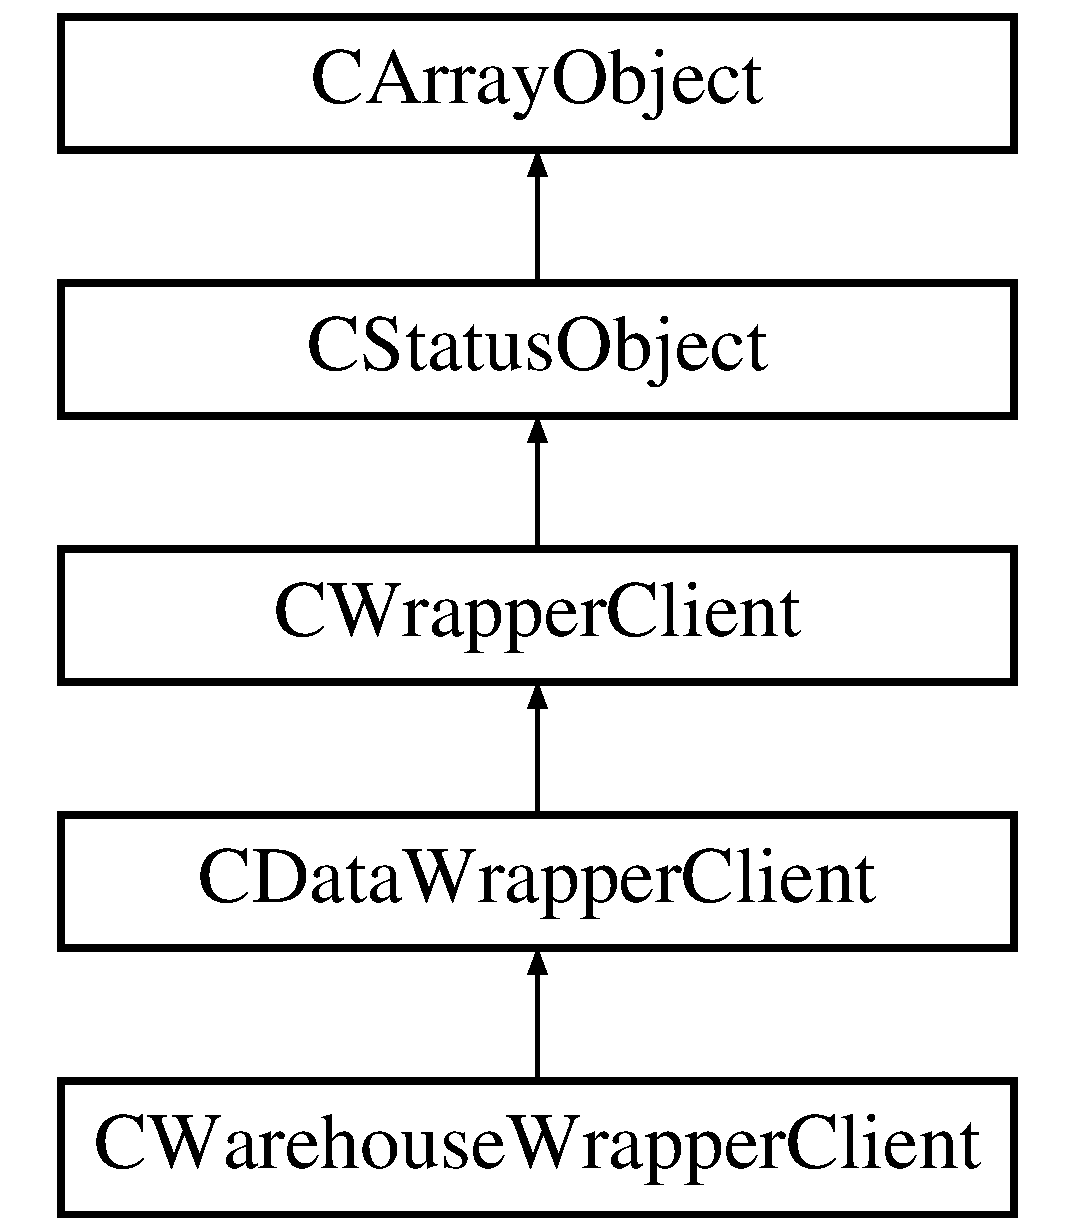
\includegraphics[height=5.000000cm]{class_c_warehouse_wrapper_client}
\end{center}
\end{figure}
\subsection*{Public Member Functions}
\begin{DoxyCompactItemize}
\item 
\hyperlink{class_c_warehouse_wrapper_client_a099ef5aef1883aa5b394c7086a818496}{Operation} (\$the\-Value=N\-U\-L\-L, \$get\-Old=F\-A\-L\-S\-E)
\item 
\hyperlink{class_c_warehouse_wrapper_client_ac953bbdc9dd6ccffa7ddfb8f59bbaf26}{User\-Code} (\$the\-Value=N\-U\-L\-L, \$get\-Old=F\-A\-L\-S\-E)
\item 
\hyperlink{class_c_warehouse_wrapper_client_a60e22139d7af5c828dcac8098e16ec6a}{User\-Pass} (\$the\-Value=N\-U\-L\-L, \$get\-Old=F\-A\-L\-S\-E)
\item 
\hyperlink{class_c_warehouse_wrapper_client_a39a624769f7cd1aebca73e7ba2c042e2}{Identifiers} (\$the\-Value=N\-U\-L\-L, \$the\-Operation=N\-U\-L\-L, \$get\-Old=F\-A\-L\-S\-E)
\item 
\hyperlink{class_c_warehouse_wrapper_client_a13557a813d85e638d97b729a27631af7}{Predicates} (\$the\-Value=N\-U\-L\-L, \$the\-Operation=N\-U\-L\-L, \$get\-Old=F\-A\-L\-S\-E)
\item 
\hyperlink{class_c_warehouse_wrapper_client_a5550bc094adb0dda32ce32979d4b70b7}{Attributes} (\$the\-Key, \$the\-Value=N\-U\-L\-L, \$the\-Operation=N\-U\-L\-L, \$get\-Old=F\-A\-L\-S\-E)
\item 
\hyperlink{class_c_warehouse_wrapper_client_a74a9e226190002542c67c64e766b91cd}{Direction} (\$the\-Value=N\-U\-L\-L, \$get\-Old=F\-A\-L\-S\-E)
\item 
\hyperlink{class_c_warehouse_wrapper_client_a858974f6dedaa731da4fe26664a21ab7}{Levels} (\$the\-Value=N\-U\-L\-L, \$get\-Old=F\-A\-L\-S\-E)
\end{DoxyCompactItemize}


\subsection{Member Function Documentation}
\hypertarget{class_c_warehouse_wrapper_client_a5550bc094adb0dda32ce32979d4b70b7}{\index{C\-Warehouse\-Wrapper\-Client@{C\-Warehouse\-Wrapper\-Client}!Attributes@{Attributes}}
\index{Attributes@{Attributes}!CWarehouseWrapperClient@{C\-Warehouse\-Wrapper\-Client}}
\subsubsection[{Attributes}]{\setlength{\rightskip}{0pt plus 5cm}C\-Warehouse\-Wrapper\-Client\-::\-Attributes (
\begin{DoxyParamCaption}
\item[{}]{\$the\-Key, }
\item[{}]{\$the\-Value = {\ttfamily NULL}, }
\item[{}]{\$the\-Operation = {\ttfamily NULL}, }
\item[{}]{\$get\-Old = {\ttfamily FALSE}}
\end{DoxyParamCaption}
)}}\label{class_c_warehouse_wrapper_client_a5550bc094adb0dda32ce32979d4b70b7}
Manage selectors list.

This method can be used to manage the \hyperlink{}{attribute} selectors, it manages the following array structure\-:


\begin{DoxyItemize}
\item {\itshape Key}\-: The array key should correspond to the node attribute you want to match\-: 
\begin{DoxyItemize}
\item {\itshape \hyperlink{}{k\-T\-A\-G\-\_\-\-T\-Y\-P\-E}}\-: The ontology node type. 
\item {\itshape \hyperlink{}{k\-T\-A\-G\-\_\-\-K\-I\-N\-D}}\-: The ontology node kind. 
\item {\itshape \hyperlink{}{k\-T\-A\-G\-\_\-\-D\-O\-M\-A\-I\-N}}\-: The domain of the ontology. 
\item {\itshape \hyperlink{}{k\-T\-A\-G\-\_\-\-C\-A\-T\-E\-G\-O\-R\-Y}}\-: The category of the ontology. 
\end{DoxyItemize}
\item {\itshape Value}\-: An array of values to be matched. 
\end{DoxyItemize}

The elements of these key/value pairs will be compared in {\itshape A\-N\-D}.

The parameters to this method are\-:


\begin{DoxyItemize}
\item {\bfseries \$the\-Key}\-: The attribute key. 
\item {\bfseries \$the\-Value}\-: The attribute value\-: 
\begin{DoxyItemize}
\item {\itshape N\-U\-L\-L}\-: Apply operation to all values. 
\item {\itshape other}\-: The attribute value. 
\end{DoxyItemize}
\item {\bfseries \$the\-Operation}\-: The operation\-: 
\begin{DoxyItemize}
\item {\itshape N\-U\-L\-L}\-: Return the attribute value matched by the first and second parameters, or return all values matching the first parameter if the second is {\itshape N\-U\-L\-L}. 
\item {\itshape F\-A\-L\-S\-E}\-: Delete the attribute value matched by the first and second parameters, or delete all values matching the first parameter if the second is {\itshape N\-U\-L\-L}. 
\item {\itshape T\-R\-U\-E}\-: Add the value in the second parameter to the attributes matching the first parameter, or replace all values matching the first parameter with the value in the second parameter. 
\end{DoxyItemize}
\end{DoxyItemize}


\begin{DoxyParams}[1]{Parameters}
mixed & {\em \$the\-Key} & Attribute key. \\
\hline
mixed & {\em \$the\-Value} & Value or index. \\
\hline
mixed & {\em \$the\-Operation} & Operation. \\
\hline
boolean & {\em \$get\-Old} & T\-R\-U\-E get old value.\\
\hline
\end{DoxyParams}
public \begin{DoxyReturn}{Returns}
mixed
\end{DoxyReturn}
\begin{DoxySeeAlso}{See also}
k\-A\-P\-I\-\_\-\-O\-P\-T\-\_\-\-A\-T\-T\-R\-I\-B\-U\-T\-E\-S 
\end{DoxySeeAlso}
\hypertarget{class_c_warehouse_wrapper_client_a74a9e226190002542c67c64e766b91cd}{\index{C\-Warehouse\-Wrapper\-Client@{C\-Warehouse\-Wrapper\-Client}!Direction@{Direction}}
\index{Direction@{Direction}!CWarehouseWrapperClient@{C\-Warehouse\-Wrapper\-Client}}
\subsubsection[{Direction}]{\setlength{\rightskip}{0pt plus 5cm}C\-Warehouse\-Wrapper\-Client\-::\-Direction (
\begin{DoxyParamCaption}
\item[{}]{\$the\-Value = {\ttfamily NULL}, }
\item[{}]{\$get\-Old = {\ttfamily FALSE}}
\end{DoxyParamCaption}
)}}\label{class_c_warehouse_wrapper_client_a74a9e226190002542c67c64e766b91cd}
Manage edges direction.

This method can be used to manage the \hyperlink{}{edges} direction, it accepts a string which represents either the relationship \hyperlink{}{direction}, or the requested operation\-:


\begin{DoxyItemize}
\item {\itshape N\-U\-L\-L}\-: Return the current value. 
\item {\itshape F\-A\-L\-S\-E}\-: Delete the current value. 
\item {\itshape other}\-: Set the value with the provided parameter\-: 
\begin{DoxyItemize}
\item {\itshape \hyperlink{}{k\-A\-P\-I\-\_\-\-D\-I\-R\-E\-C\-T\-I\-O\-N\-\_\-\-I\-N}}\-: Incoming relationships. 
\item {\itshape \hyperlink{}{k\-A\-P\-I\-\_\-\-D\-I\-R\-E\-C\-T\-I\-O\-N\-\_\-\-O\-U\-T}}\-: Outgoing relationships. 
\item {\itshape \hyperlink{}{k\-A\-P\-I\-\_\-\-D\-I\-R\-E\-C\-T\-I\-O\-N\-\_\-\-A\-L\-L}}\-: Both incoming and outgoing relationships. 
\end{DoxyItemize}
\end{DoxyItemize}

The second parameter is a boolean which if {\itshape T\-R\-U\-E} will return the {\itshape old} value when replacing values; if {\itshape F\-A\-L\-S\-E}, it will return the currently set value.


\begin{DoxyParams}[1]{Parameters}
integer & {\em \$the\-Value} & Value or operation. \\
\hline
boolean & {\em \$get\-Old} & T\-R\-U\-E get old value.\\
\hline
\end{DoxyParams}
public \begin{DoxyReturn}{Returns}
mixed
\end{DoxyReturn}
\hyperlink{class_c_attribute_a9d231a47718719fcd6c33f3d0ac91675}{C\-Attribute\-::\-Manage\-Offset()}

\begin{DoxySeeAlso}{See also}
k\-A\-P\-I\-\_\-\-O\-P\-T\-\_\-\-D\-I\-R\-E\-C\-T\-I\-O\-N 
\end{DoxySeeAlso}
\hypertarget{class_c_warehouse_wrapper_client_a39a624769f7cd1aebca73e7ba2c042e2}{\index{C\-Warehouse\-Wrapper\-Client@{C\-Warehouse\-Wrapper\-Client}!Identifiers@{Identifiers}}
\index{Identifiers@{Identifiers}!CWarehouseWrapperClient@{C\-Warehouse\-Wrapper\-Client}}
\subsubsection[{Identifiers}]{\setlength{\rightskip}{0pt plus 5cm}C\-Warehouse\-Wrapper\-Client\-::\-Identifiers (
\begin{DoxyParamCaption}
\item[{}]{\$the\-Value = {\ttfamily NULL}, }
\item[{}]{\$the\-Operation = {\ttfamily NULL}, }
\item[{}]{\$get\-Old = {\ttfamily FALSE}}
\end{DoxyParamCaption}
)}}\label{class_c_warehouse_wrapper_client_a39a624769f7cd1aebca73e7ba2c042e2}
Manage identifiers list.

This method can be used to manage the \hyperlink{}{identifiers}, it uses the standard accessor \hyperlink{class_c_attribute_a7d2e35b120eaa55529f78253f77dab48}{method} to manage the list of identifiers.

For a more thorough reference of how this method works, please consult the \hyperlink{class_c_attribute_a7d2e35b120eaa55529f78253f77dab48}{C\-Attribute\-::\-Manage\-Array\-Offset} method, in which the second parameter will be the constant \hyperlink{}{k\-A\-P\-I\-\_\-\-O\-P\-T\-\_\-\-I\-D\-E\-N\-T\-I\-F\-I\-E\-R\-S}.


\begin{DoxyParams}[1]{Parameters}
mixed & {\em \$the\-Value} & Value or index. \\
\hline
mixed & {\em \$the\-Operation} & Operation. \\
\hline
boolean & {\em \$get\-Old} & T\-R\-U\-E get old value.\\
\hline
\end{DoxyParams}
public \begin{DoxyReturn}{Returns}
mixed
\end{DoxyReturn}
\hyperlink{class_c_attribute_a7d2e35b120eaa55529f78253f77dab48}{C\-Attribute\-::\-Manage\-Array\-Offset()}

\begin{DoxySeeAlso}{See also}
k\-A\-P\-I\-\_\-\-O\-P\-T\-\_\-\-I\-D\-E\-N\-T\-I\-F\-I\-E\-R\-S 
\end{DoxySeeAlso}
\hypertarget{class_c_warehouse_wrapper_client_a858974f6dedaa731da4fe26664a21ab7}{\index{C\-Warehouse\-Wrapper\-Client@{C\-Warehouse\-Wrapper\-Client}!Levels@{Levels}}
\index{Levels@{Levels}!CWarehouseWrapperClient@{C\-Warehouse\-Wrapper\-Client}}
\subsubsection[{Levels}]{\setlength{\rightskip}{0pt plus 5cm}C\-Warehouse\-Wrapper\-Client\-::\-Levels (
\begin{DoxyParamCaption}
\item[{}]{\$the\-Value = {\ttfamily NULL}, }
\item[{}]{\$get\-Old = {\ttfamily FALSE}}
\end{DoxyParamCaption}
)}}\label{class_c_warehouse_wrapper_client_a858974f6dedaa731da4fe26664a21ab7}
Manage traversal depts level.

This method can be used to manage the \hyperlink{}{levels} of depth in graph \hyperlink{}{traversals}, it accepts an integer which represents the number of levels to traverse; if the value is negative, all levels will be traversed.


\begin{DoxyItemize}
\item {\itshape N\-U\-L\-L}\-: Return the current value. 
\item {\itshape F\-A\-L\-S\-E}\-: Delete the current value. 
\item {\itshape other}\-: Set the value with the provided parameter. 
\end{DoxyItemize}

The second parameter is a boolean which if {\itshape T\-R\-U\-E} will return the {\itshape old} value when replacing values; if {\itshape F\-A\-L\-S\-E}, it will return the currently set value.


\begin{DoxyParams}[1]{Parameters}
integer & {\em \$the\-Value} & Value or operation. \\
\hline
boolean & {\em \$get\-Old} & T\-R\-U\-E get old value.\\
\hline
\end{DoxyParams}
public \begin{DoxyReturn}{Returns}
mixed
\end{DoxyReturn}
\hyperlink{class_c_attribute_a9d231a47718719fcd6c33f3d0ac91675}{C\-Attribute\-::\-Manage\-Offset()}

\begin{DoxySeeAlso}{See also}
k\-A\-P\-I\-\_\-\-O\-P\-T\-\_\-\-L\-E\-V\-E\-L\-S 
\end{DoxySeeAlso}
\hypertarget{class_c_warehouse_wrapper_client_a099ef5aef1883aa5b394c7086a818496}{\index{C\-Warehouse\-Wrapper\-Client@{C\-Warehouse\-Wrapper\-Client}!Operation@{Operation}}
\index{Operation@{Operation}!CWarehouseWrapperClient@{C\-Warehouse\-Wrapper\-Client}}
\subsubsection[{Operation}]{\setlength{\rightskip}{0pt plus 5cm}C\-Warehouse\-Wrapper\-Client\-::\-Operation (
\begin{DoxyParamCaption}
\item[{}]{\$the\-Value = {\ttfamily NULL}, }
\item[{}]{\$get\-Old = {\ttfamily FALSE}}
\end{DoxyParamCaption}
)}}\label{class_c_warehouse_wrapper_client_a099ef5aef1883aa5b394c7086a818496}
Manage operation.

We \hyperlink{class_c_data_wrapper_client_ae7cad4809c20d8f2871cfe00da909d67}{overload} this method to add the following allowed operations\-:


\begin{DoxyItemize}
\item {\itshape \hyperlink{}{k\-A\-P\-I\-\_\-\-O\-P\-\_\-\-L\-O\-G\-I\-N}}\-: This is the tag that represents the user login operation, it will return the \hyperlink{class_c_user}{user} matching the provided user \hyperlink{class_c_warehouse_wrapper_client_ac953bbdc9dd6ccffa7ddfb8f59bbaf26}{code} and \hyperlink{class_c_warehouse_wrapper_client_a60e22139d7af5c828dcac8098e16ec6a}{password}. 
\end{DoxyItemize}


\begin{DoxyParams}[1]{Parameters}
string & {\em \$the\-Value} & Value or operation. \\
\hline
boolean & {\em \$get\-Old} & T\-R\-U\-E get old value.\\
\hline
\end{DoxyParams}
public \begin{DoxyReturn}{Returns}
mixed
\end{DoxyReturn}

\begin{DoxyExceptions}{Exceptions}
{\em \{@link} & \hyperlink{class_c_exception}{C\-Exception} \hyperlink{class_c_exception}{C\-Exception}\}\\
\hline
\end{DoxyExceptions}
\hyperlink{class_c_attribute_a9d231a47718719fcd6c33f3d0ac91675}{C\-Attribute\-::\-Manage\-Offset()}

\begin{DoxySeeAlso}{See also}
k\-A\-P\-I\-\_\-\-O\-P\-E\-R\-A\-T\-I\-O\-N 

k\-A\-P\-I\-\_\-\-O\-P\-\_\-\-G\-E\-T\-\_\-\-O\-N\-E k\-A\-P\-I\-\_\-\-O\-P\-\_\-\-G\-E\-T\-\_\-\-O\-B\-J\-E\-C\-T\-\_\-\-R\-E\-F 
\end{DoxySeeAlso}


Reimplemented from \hyperlink{class_c_data_wrapper_client_ae7cad4809c20d8f2871cfe00da909d67}{C\-Data\-Wrapper\-Client}.

\hypertarget{class_c_warehouse_wrapper_client_a13557a813d85e638d97b729a27631af7}{\index{C\-Warehouse\-Wrapper\-Client@{C\-Warehouse\-Wrapper\-Client}!Predicates@{Predicates}}
\index{Predicates@{Predicates}!CWarehouseWrapperClient@{C\-Warehouse\-Wrapper\-Client}}
\subsubsection[{Predicates}]{\setlength{\rightskip}{0pt plus 5cm}C\-Warehouse\-Wrapper\-Client\-::\-Predicates (
\begin{DoxyParamCaption}
\item[{}]{\$the\-Value = {\ttfamily NULL}, }
\item[{}]{\$the\-Operation = {\ttfamily NULL}, }
\item[{}]{\$get\-Old = {\ttfamily FALSE}}
\end{DoxyParamCaption}
)}}\label{class_c_warehouse_wrapper_client_a13557a813d85e638d97b729a27631af7}
Manage predicates list.

This method can be used to manage the \hyperlink{}{predicates}, it uses the standard accessor \hyperlink{class_c_attribute_a7d2e35b120eaa55529f78253f77dab48}{method} to manage the list of predicates.

For a more thorough reference of how this method works, please consult the \hyperlink{class_c_attribute_a7d2e35b120eaa55529f78253f77dab48}{C\-Attribute\-::\-Manage\-Array\-Offset} method, in which the second parameter will be the constant \hyperlink{}{k\-A\-P\-I\-\_\-\-O\-P\-T\-\_\-\-P\-R\-E\-D\-I\-C\-A\-T\-E\-S}.


\begin{DoxyParams}[1]{Parameters}
mixed & {\em \$the\-Value} & Value or index. \\
\hline
mixed & {\em \$the\-Operation} & Operation. \\
\hline
boolean & {\em \$get\-Old} & T\-R\-U\-E get old value.\\
\hline
\end{DoxyParams}
public \begin{DoxyReturn}{Returns}
mixed
\end{DoxyReturn}
\hyperlink{class_c_attribute_a7d2e35b120eaa55529f78253f77dab48}{C\-Attribute\-::\-Manage\-Array\-Offset()}

\begin{DoxySeeAlso}{See also}
k\-A\-P\-I\-\_\-\-O\-P\-T\-\_\-\-P\-R\-E\-D\-I\-C\-A\-T\-E\-S 
\end{DoxySeeAlso}
\hypertarget{class_c_warehouse_wrapper_client_ac953bbdc9dd6ccffa7ddfb8f59bbaf26}{\index{C\-Warehouse\-Wrapper\-Client@{C\-Warehouse\-Wrapper\-Client}!User\-Code@{User\-Code}}
\index{User\-Code@{User\-Code}!CWarehouseWrapperClient@{C\-Warehouse\-Wrapper\-Client}}
\subsubsection[{User\-Code}]{\setlength{\rightskip}{0pt plus 5cm}C\-Warehouse\-Wrapper\-Client\-::\-User\-Code (
\begin{DoxyParamCaption}
\item[{}]{\$the\-Value = {\ttfamily NULL}, }
\item[{}]{\$get\-Old = {\ttfamily FALSE}}
\end{DoxyParamCaption}
)}}\label{class_c_warehouse_wrapper_client_ac953bbdc9dd6ccffa7ddfb8f59bbaf26}
Manage user code.

This method can be used to manage the user \hyperlink{}{code}, it accepts a string which represents either the user code, or the requested operation\-:


\begin{DoxyItemize}
\item {\itshape N\-U\-L\-L}\-: Return the current value. 
\item {\itshape F\-A\-L\-S\-E}\-: Delete the current value. 
\item {\itshape other}\-: Set the value with the provided parameter. 
\end{DoxyItemize}

The second parameter is a boolean which if {\itshape T\-R\-U\-E} will return the {\itshape old} value when replacing values; if {\itshape F\-A\-L\-S\-E}, it will return the currently set value.


\begin{DoxyParams}[1]{Parameters}
integer & {\em \$the\-Value} & Value or operation. \\
\hline
boolean & {\em \$get\-Old} & T\-R\-U\-E get old value.\\
\hline
\end{DoxyParams}
public \begin{DoxyReturn}{Returns}
mixed
\end{DoxyReturn}
\hyperlink{class_c_attribute_a9d231a47718719fcd6c33f3d0ac91675}{C\-Attribute\-::\-Manage\-Offset()}

\begin{DoxySeeAlso}{See also}
k\-A\-P\-I\-\_\-\-O\-P\-T\-\_\-\-U\-S\-E\-R\-\_\-\-C\-O\-D\-E 
\end{DoxySeeAlso}
\hypertarget{class_c_warehouse_wrapper_client_a60e22139d7af5c828dcac8098e16ec6a}{\index{C\-Warehouse\-Wrapper\-Client@{C\-Warehouse\-Wrapper\-Client}!User\-Pass@{User\-Pass}}
\index{User\-Pass@{User\-Pass}!CWarehouseWrapperClient@{C\-Warehouse\-Wrapper\-Client}}
\subsubsection[{User\-Pass}]{\setlength{\rightskip}{0pt plus 5cm}C\-Warehouse\-Wrapper\-Client\-::\-User\-Pass (
\begin{DoxyParamCaption}
\item[{}]{\$the\-Value = {\ttfamily NULL}, }
\item[{}]{\$get\-Old = {\ttfamily FALSE}}
\end{DoxyParamCaption}
)}}\label{class_c_warehouse_wrapper_client_a60e22139d7af5c828dcac8098e16ec6a}
Manage user password.

This method can be used to manage the user \hyperlink{}{password}, it accepts a string which represents either the user password, or the requested operation\-:


\begin{DoxyItemize}
\item {\itshape N\-U\-L\-L}\-: Return the current value. 
\item {\itshape F\-A\-L\-S\-E}\-: Delete the current value. 
\item {\itshape other}\-: Set the value with the provided parameter. 
\end{DoxyItemize}

The second parameter is a boolean which if {\itshape T\-R\-U\-E} will return the {\itshape old} value when replacing values; if {\itshape F\-A\-L\-S\-E}, it will return the currently set value.


\begin{DoxyParams}[1]{Parameters}
integer & {\em \$the\-Value} & Value or operation. \\
\hline
boolean & {\em \$get\-Old} & T\-R\-U\-E get old value.\\
\hline
\end{DoxyParams}
public \begin{DoxyReturn}{Returns}
mixed
\end{DoxyReturn}
\hyperlink{class_c_attribute_a9d231a47718719fcd6c33f3d0ac91675}{C\-Attribute\-::\-Manage\-Offset()}

\begin{DoxySeeAlso}{See also}
k\-A\-P\-I\-\_\-\-O\-P\-T\-\_\-\-U\-S\-E\-R\-\_\-\-P\-A\-S\-S 
\end{DoxySeeAlso}


The documentation for this class was generated from the following file\-:\begin{DoxyCompactItemize}
\item 
/\-Library/\-Web\-Server/\-Library/wrapper/classes/C\-Warehouse\-Wrapper\-Client.\-php\end{DoxyCompactItemize}

\hypertarget{class_c_wrapper}{\section{C\-Wrapper Class Reference}
\label{class_c_wrapper}\index{C\-Wrapper@{C\-Wrapper}}
}
Inheritance diagram for C\-Wrapper\-:\begin{figure}[H]
\begin{center}
\leavevmode
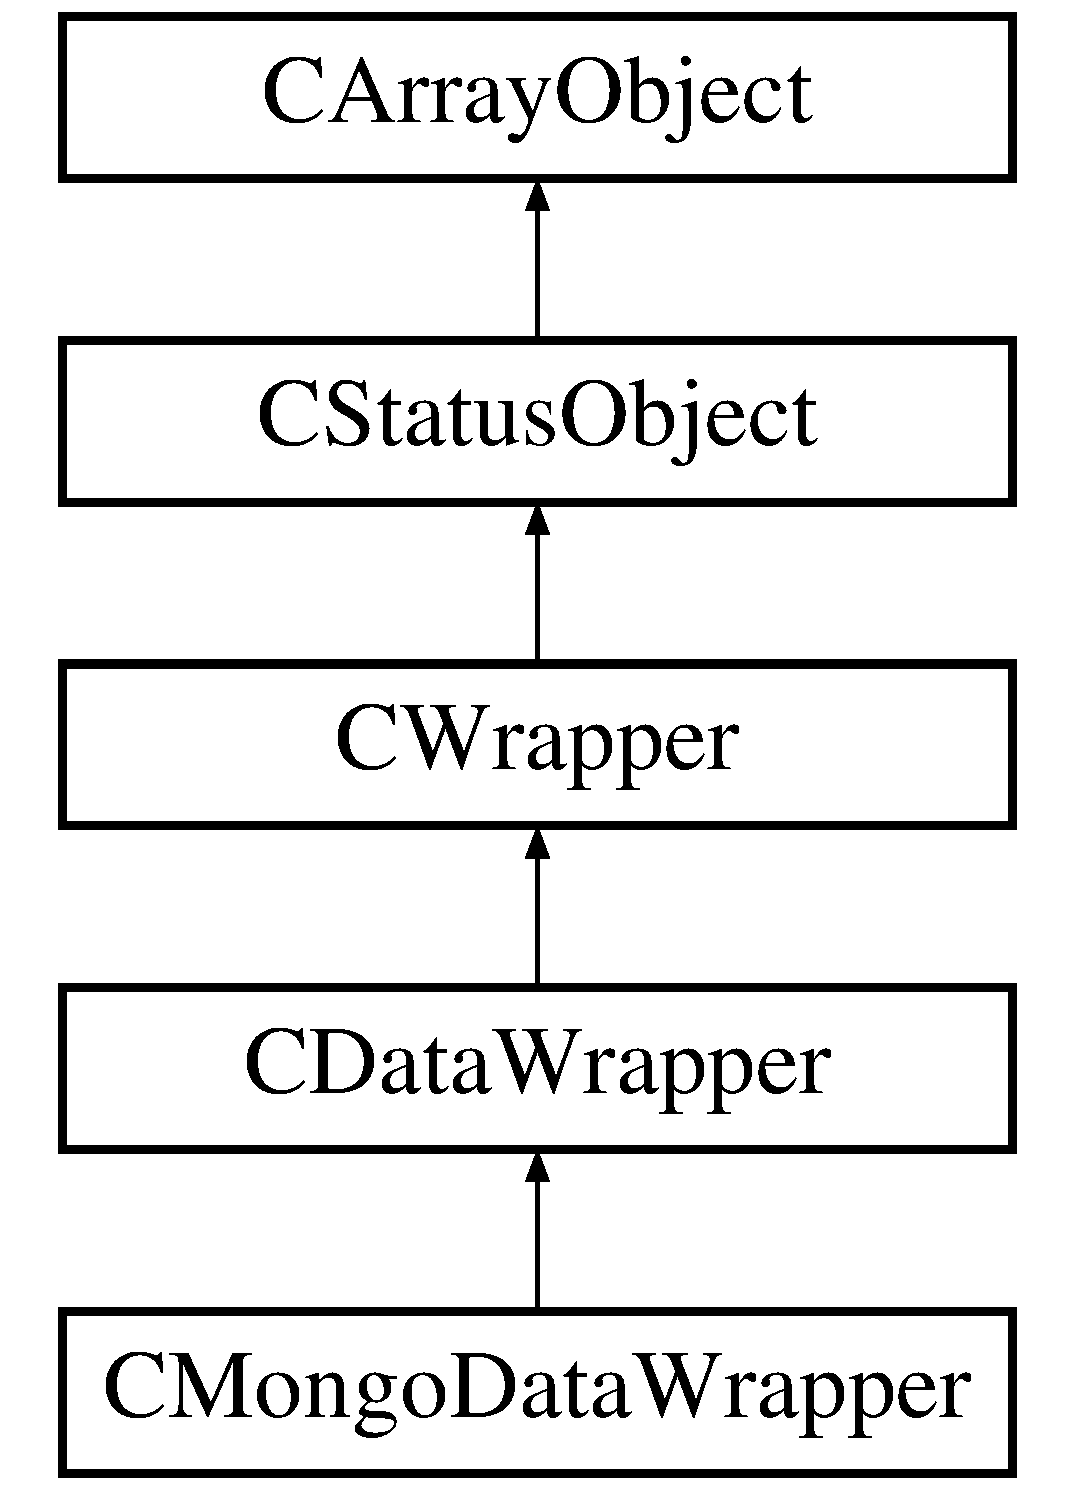
\includegraphics[height=6.000000cm]{class_c_wrapper}
\end{center}
\end{figure}
\subsection*{Public Member Functions}
\begin{DoxyCompactItemize}
\item 
\hyperlink{class_c_wrapper_a683094b01e0682fd34926562d7a052e0}{\-\_\-\-\_\-construct} ()
\item 
\hyperlink{class_c_wrapper_a0e605ca2cdd718ecdeb6f3be9b1f0162}{Handle\-Request} ()
\end{DoxyCompactItemize}
\subsection*{Protected Member Functions}
\begin{DoxyCompactItemize}
\item 
\hyperlink{class_c_wrapper_a8369eec2e53b3f6394a35bcd919d8779}{\-\_\-\-Init\-Status} ()
\item 
\hyperlink{class_c_wrapper_aec2fa3594e36a380d66743b47c24490c}{\-\_\-\-Init\-Options} ()
\item 
\hyperlink{class_c_wrapper_a0e5c5488fce4b388e43dcf6810874d74}{\-\_\-\-Init\-Resources} ()
\item 
\hyperlink{class_c_wrapper_a6675c744053f1b05547ad28fc50a79e6}{\-\_\-\-Parse\-Request} ()
\item 
\hyperlink{class_c_wrapper_a2a3d95961650654468789883ab1607e5}{\-\_\-\-Format\-Request} ()
\item 
\hyperlink{class_c_wrapper_a24b22cfd0022c1cba1741fb294fba5ba}{\-\_\-\-Validate\-Request} ()
\item 
\hyperlink{class_c_wrapper_a53d59f3a61137b8d6f5707d794e2961a}{\-\_\-\-Parse\-Format} ()
\item 
\hyperlink{class_c_wrapper_aa090c135ca1085f46d8cddd393131ea6}{\-\_\-\-Parse\-Operation} ()
\item 
\hyperlink{class_c_wrapper_a13421345af75888b1fa8bcd3381b52a5}{\-\_\-\-Parse\-Timing} ()
\item 
\hyperlink{class_c_wrapper_a8994ff7a5f94438da1c5e3505b145dbd}{\-\_\-\-Validate\-Format} ()
\item 
\hyperlink{class_c_wrapper_aab3f7b2ca4cd9e692c35510d753918a4}{\-\_\-\-Validate\-Operation} ()
\item 
\hyperlink{class_c_wrapper_a12c1dd1f1d1cf0ae889cc19ff17ced0e}{\-\_\-\-Handle\-Request} ()
\item 
\hyperlink{class_c_wrapper_aeff4d2ab12617c1dda2bed705a6969bb}{\-\_\-\-Handle\-\_\-\-List\-Op} (\&\$the\-List)
\item 
\hyperlink{class_c_wrapper_ab58ee7076059e0f992c2a642043b764f}{\-\_\-\-Handle\-\_\-\-Ping} ()
\item 
\hyperlink{class_c_wrapper_aff9eb1799c8f30cb33967c7a50ce6395}{\-\_\-\-Offset\-Manage} (\$the\-Block, \$the\-Element, \$the\-Value=N\-U\-L\-L)
\item 
\hyperlink{class_c_wrapper_ad8dd05c155df0d8fe19be35d4bb67b56}{\-\_\-\-Exception2\-Status} (Exception \$the\-Exception)
\item 
\hyperlink{class_c_wrapper_a60583bacf329d484d01df9851602759f}{\-\_\-\-Encode\-Response} ()
\end{DoxyCompactItemize}
\subsection*{Protected Attributes}
\begin{DoxyCompactItemize}
\item 
\hypertarget{class_c_wrapper_ad9a1a67bf2f21f3b4d0cd83b19be31e3}{{\bfseries \$m\-Received\-Stamp} = N\-U\-L\-L}\label{class_c_wrapper_ad9a1a67bf2f21f3b4d0cd83b19be31e3}

\end{DoxyCompactItemize}


\subsection{Constructor \& Destructor Documentation}
\hypertarget{class_c_wrapper_a683094b01e0682fd34926562d7a052e0}{\index{C\-Wrapper@{C\-Wrapper}!\-\_\-\-\_\-construct@{\-\_\-\-\_\-construct}}
\index{\-\_\-\-\_\-construct@{\-\_\-\-\_\-construct}!CWrapper@{C\-Wrapper}}
\subsubsection[{\-\_\-\-\_\-construct}]{\setlength{\rightskip}{0pt plus 5cm}C\-Wrapper\-::\-\_\-\-\_\-construct (
\begin{DoxyParamCaption}
{}
\end{DoxyParamCaption}
)}}\label{class_c_wrapper_a683094b01e0682fd34926562d7a052e0}
Instantiate class.

The constructor will set-\/up the environment and parse the request. The workflow is as follows\-:


\begin{DoxyItemize}
\item {\itshape Check required elements}\-: The method will check if all required elements of the request are there, only if this is the case will the constructor init the service. 
\item {\itshape Init \hyperlink{class_c_wrapper_a8369eec2e53b3f6394a35bcd919d8779}{status}}\-: The response status will be initialised to the \hyperlink{}{idle} state. 
\item {\itshape Init \hyperlink{class_c_wrapper_aec2fa3594e36a380d66743b47c24490c}{options}}\-: Service options will be initialised. 
\item {\itshape Init \hyperlink{class_c_wrapper_a0e5c5488fce4b388e43dcf6810874d74}{resources}}\-: Eventual resources are initialised. 
\item {\itshape \hyperlink{class_c_wrapper_a6675c744053f1b05547ad28fc50a79e6}{Parse} request}\-: The request is parsed. 
\item {\itshape \hyperlink{class_c_wrapper_a2a3d95961650654468789883ab1607e5}{Format} request}\-: The request is normalised if necessary. 
\item {\itshape \hyperlink{class_c_wrapper_a24b22cfd0022c1cba1741fb294fba5ba}{Validate} request}\-: The request is validated. 
\end{DoxyItemize}

This protected interface should be overloaded by derived classes to implement custom services.

public

\hyperlink{class_c_wrapper_a8369eec2e53b3f6394a35bcd919d8779}{\-\_\-\-Init\-Status()}  \hyperlink{class_c_wrapper_aec2fa3594e36a380d66743b47c24490c}{\-\_\-\-Init\-Options()}  \hyperlink{class_c_wrapper_a0e5c5488fce4b388e43dcf6810874d74}{\-\_\-\-Init\-Resources()}  \hyperlink{class_c_wrapper_a6675c744053f1b05547ad28fc50a79e6}{\-\_\-\-Parse\-Request()}  \hyperlink{class_c_wrapper_a2a3d95961650654468789883ab1607e5}{\-\_\-\-Format\-Request()}  \hyperlink{class_c_wrapper_a24b22cfd0022c1cba1741fb294fba5ba}{\-\_\-\-Validate\-Request()}  \hyperlink{class_c_wrapper_ad8dd05c155df0d8fe19be35d4bb67b56}{\-\_\-\-Exception2\-Status()}  \hyperlink{class_c_wrapper_a60583bacf329d484d01df9851602759f}{\-\_\-\-Encode\-Response()} 

\subsection{Member Function Documentation}
\hypertarget{class_c_wrapper_a60583bacf329d484d01df9851602759f}{\index{C\-Wrapper@{C\-Wrapper}!\-\_\-\-Encode\-Response@{\-\_\-\-Encode\-Response}}
\index{\-\_\-\-Encode\-Response@{\-\_\-\-Encode\-Response}!CWrapper@{C\-Wrapper}}
\subsubsection[{\-\_\-\-Encode\-Response}]{\setlength{\rightskip}{0pt plus 5cm}C\-Wrapper\-::\-\_\-\-Encode\-Response (
\begin{DoxyParamCaption}
{}
\end{DoxyParamCaption}
)\hspace{0.3cm}{\ttfamily [protected]}}}\label{class_c_wrapper_a60583bacf329d484d01df9851602759f}
Encode response.

This method will return the encoded response string.

protected \begin{DoxyReturn}{Returns}
string$|$\-N\-U\-L\-L 
\end{DoxyReturn}
\hypertarget{class_c_wrapper_ad8dd05c155df0d8fe19be35d4bb67b56}{\index{C\-Wrapper@{C\-Wrapper}!\-\_\-\-Exception2\-Status@{\-\_\-\-Exception2\-Status}}
\index{\-\_\-\-Exception2\-Status@{\-\_\-\-Exception2\-Status}!CWrapper@{C\-Wrapper}}
\subsubsection[{\-\_\-\-Exception2\-Status}]{\setlength{\rightskip}{0pt plus 5cm}C\-Wrapper\-::\-\_\-\-Exception2\-Status (
\begin{DoxyParamCaption}
\item[{Exception}]{\$the\-Exception}
\end{DoxyParamCaption}
)\hspace{0.3cm}{\ttfamily [protected]}}}\label{class_c_wrapper_ad8dd05c155df0d8fe19be35d4bb67b56}
Set status from exception.

This method can be used to set the service status according to an exception\-:


\begin{DoxyItemize}
\item {\itshape \hyperlink{class_c_exception_a2bef90da8a35e80dda8072d4f748ec20}{Severity}}\-: This value will be set as the status \hyperlink{}{status}. 
\item {\itshape \hyperlink{}{Code}}\-: This value will be set as the status \hyperlink{}{code}. 
\item {\itshape \hyperlink{}{Message}}\-: This value will be set in the status \hyperlink{}{description} field as a language block. 
\item {\itshape \hyperlink{}{File}}\-: This value will be set in the status \hyperlink{}{annotations}. 
\item {\itshape \hyperlink{}{Line}}\-: This value will be set in the status \hyperlink{}{annotations}. 
\item {\itshape \hyperlink{}{Trace}}\-: This value will be set in the status \hyperlink{}{annotations}. 
\item {\itshape \hyperlink{class_c_exception_abcbd46a262790fcbe3493e30a6418821}{References}}\-: These valuew will be set in the status \hyperlink{}{annotations}. 
\end{DoxyItemize}


\begin{DoxyParams}[1]{Parameters}
Exception & {\em \$the\-Exception} & Exception.\\
\hline
\end{DoxyParams}
protected \hypertarget{class_c_wrapper_a2a3d95961650654468789883ab1607e5}{\index{C\-Wrapper@{C\-Wrapper}!\-\_\-\-Format\-Request@{\-\_\-\-Format\-Request}}
\index{\-\_\-\-Format\-Request@{\-\_\-\-Format\-Request}!CWrapper@{C\-Wrapper}}
\subsubsection[{\-\_\-\-Format\-Request}]{\setlength{\rightskip}{0pt plus 5cm}C\-Wrapper\-::\-\_\-\-Format\-Request (
\begin{DoxyParamCaption}
{}
\end{DoxyParamCaption}
)\hspace{0.3cm}{\ttfamily [protected]}}}\label{class_c_wrapper_a2a3d95961650654468789883ab1607e5}
Format request.

This method should perform any needed formatting before the request will be handled.

In this class we do nothing.

protected 

Reimplemented in \hyperlink{class_c_data_wrapper_ab46c0e9797e8636ca1c9d535b377b90a}{C\-Data\-Wrapper}, \hyperlink{class_c_warehouse_wrapper_a4bd0282949f52ce148b60218c48ddde5}{C\-Warehouse\-Wrapper}, and \hyperlink{class_c_mongo_data_wrapper_abbc0d41394dda4a27eefa8481065749a}{C\-Mongo\-Data\-Wrapper}.

\hypertarget{class_c_wrapper_aeff4d2ab12617c1dda2bed705a6969bb}{\index{C\-Wrapper@{C\-Wrapper}!\-\_\-\-Handle\-\_\-\-List\-Op@{\-\_\-\-Handle\-\_\-\-List\-Op}}
\index{\-\_\-\-Handle\-\_\-\-List\-Op@{\-\_\-\-Handle\-\_\-\-List\-Op}!CWrapper@{C\-Wrapper}}
\subsubsection[{\-\_\-\-Handle\-\_\-\-List\-Op}]{\setlength{\rightskip}{0pt plus 5cm}C\-Wrapper\-::\-\_\-\-Handle\-\_\-\-List\-Op (
\begin{DoxyParamCaption}
\item[{\&}]{\$the\-List}
\end{DoxyParamCaption}
)\hspace{0.3cm}{\ttfamily [protected]}}}\label{class_c_wrapper_aeff4d2ab12617c1dda2bed705a6969bb}
Handle \hyperlink{}{list} operations request.

This method will handle the \hyperlink{}{k\-A\-P\-I\-\_\-\-O\-P\-\_\-\-H\-E\-L\-P} request, which should return the list of supported operations.


\begin{DoxyParams}[1]{Parameters}
reference & {\em \$the\-List} & Receives operations list.\\
\hline
\end{DoxyParams}
protected 

Reimplemented in \hyperlink{class_c_warehouse_wrapper_a9800cf5ca4bb22cd96a94ef542010adf}{C\-Warehouse\-Wrapper}, \hyperlink{class_c_data_wrapper_afc7251c3aad9141599372d6b94904498}{C\-Data\-Wrapper}, and \hyperlink{class_c_mongo_data_wrapper_a1ca51f95510a94bf26e004ef2e8e8d37}{C\-Mongo\-Data\-Wrapper}.

\hypertarget{class_c_wrapper_ab58ee7076059e0f992c2a642043b764f}{\index{C\-Wrapper@{C\-Wrapper}!\-\_\-\-Handle\-\_\-\-Ping@{\-\_\-\-Handle\-\_\-\-Ping}}
\index{\-\_\-\-Handle\-\_\-\-Ping@{\-\_\-\-Handle\-\_\-\-Ping}!CWrapper@{C\-Wrapper}}
\subsubsection[{\-\_\-\-Handle\-\_\-\-Ping}]{\setlength{\rightskip}{0pt plus 5cm}C\-Wrapper\-::\-\_\-\-Handle\-\_\-\-Ping (
\begin{DoxyParamCaption}
{}
\end{DoxyParamCaption}
)\hspace{0.3cm}{\ttfamily [protected]}}}\label{class_c_wrapper_ab58ee7076059e0f992c2a642043b764f}
Handle \hyperlink{}{ping} request.

This method will handle the \hyperlink{}{k\-A\-P\-I\-\_\-\-O\-P\-\_\-\-P\-I\-N\-G} request, which can be used to check if a service is alive.

The ping request will return by default the \hyperlink{}{status} block.

protected \hypertarget{class_c_wrapper_a12c1dd1f1d1cf0ae889cc19ff17ced0e}{\index{C\-Wrapper@{C\-Wrapper}!\-\_\-\-Handle\-Request@{\-\_\-\-Handle\-Request}}
\index{\-\_\-\-Handle\-Request@{\-\_\-\-Handle\-Request}!CWrapper@{C\-Wrapper}}
\subsubsection[{\-\_\-\-Handle\-Request}]{\setlength{\rightskip}{0pt plus 5cm}C\-Wrapper\-::\-\_\-\-Handle\-Request (
\begin{DoxyParamCaption}
{}
\end{DoxyParamCaption}
)\hspace{0.3cm}{\ttfamily [protected]}}}\label{class_c_wrapper_a12c1dd1f1d1cf0ae889cc19ff17ced0e}
Handle request.

This method will handle the request.

protected

\hyperlink{class_c_wrapper_aeff4d2ab12617c1dda2bed705a6969bb}{\-\_\-\-Handle\-\_\-\-List\-Op()}

\begin{DoxySeeAlso}{See Also}
k\-A\-P\-I\-\_\-\-O\-P\-\_\-\-H\-E\-L\-P k\-A\-P\-I\-\_\-\-O\-P\-\_\-\-P\-I\-N\-G 
\end{DoxySeeAlso}


Reimplemented in \hyperlink{class_c_warehouse_wrapper_a4b909b5b4aba967200ff72e3e6924b5e}{C\-Warehouse\-Wrapper}, and \hyperlink{class_c_mongo_data_wrapper_a811af7e7574a459bc56afa3afa99e1a8}{C\-Mongo\-Data\-Wrapper}.

\hypertarget{class_c_wrapper_aec2fa3594e36a380d66743b47c24490c}{\index{C\-Wrapper@{C\-Wrapper}!\-\_\-\-Init\-Options@{\-\_\-\-Init\-Options}}
\index{\-\_\-\-Init\-Options@{\-\_\-\-Init\-Options}!CWrapper@{C\-Wrapper}}
\subsubsection[{\-\_\-\-Init\-Options}]{\setlength{\rightskip}{0pt plus 5cm}C\-Wrapper\-::\-\_\-\-Init\-Options (
\begin{DoxyParamCaption}
{}
\end{DoxyParamCaption}
)\hspace{0.3cm}{\ttfamily [protected]}}}\label{class_c_wrapper_aec2fa3594e36a380d66743b47c24490c}
Initialise options.

This method is responsible for parsing and setting all default and provided options, derived classes should overload this method to handle custom options.

In this class we initialise the \hyperlink{}{request} and \hyperlink{}{timer} sections if required.

protected

\begin{DoxySeeAlso}{See Also}
k\-A\-P\-I\-\_\-\-D\-A\-T\-A\-\_\-\-R\-E\-Q\-U\-E\-S\-T k\-A\-P\-I\-\_\-\-D\-A\-T\-A\-\_\-\-T\-I\-M\-I\-N\-G 
\end{DoxySeeAlso}


Reimplemented in \hyperlink{class_c_data_wrapper_a85c97add738d08f2f2a9958ffbda6c03}{C\-Data\-Wrapper}, and \hyperlink{class_c_warehouse_wrapper_a8dd1de1d5595647b0999ffa6b658c605}{C\-Warehouse\-Wrapper}.

\hypertarget{class_c_wrapper_a0e5c5488fce4b388e43dcf6810874d74}{\index{C\-Wrapper@{C\-Wrapper}!\-\_\-\-Init\-Resources@{\-\_\-\-Init\-Resources}}
\index{\-\_\-\-Init\-Resources@{\-\_\-\-Init\-Resources}!CWrapper@{C\-Wrapper}}
\subsubsection[{\-\_\-\-Init\-Resources}]{\setlength{\rightskip}{0pt plus 5cm}C\-Wrapper\-::\-\_\-\-Init\-Resources (
\begin{DoxyParamCaption}
{}
\end{DoxyParamCaption}
)\hspace{0.3cm}{\ttfamily [protected]}}}\label{class_c_wrapper_a0e5c5488fce4b388e43dcf6810874d74}
Initialise resources.

In derived classes this should be the method that initialises the data store resources, in this class we have no resources.

protected 

Reimplemented in \hyperlink{class_c_mongo_data_wrapper_a33ff97c26b97d00a67f97d41f67ce47b}{C\-Mongo\-Data\-Wrapper}.

\hypertarget{class_c_wrapper_a8369eec2e53b3f6394a35bcd919d8779}{\index{C\-Wrapper@{C\-Wrapper}!\-\_\-\-Init\-Status@{\-\_\-\-Init\-Status}}
\index{\-\_\-\-Init\-Status@{\-\_\-\-Init\-Status}!CWrapper@{C\-Wrapper}}
\subsubsection[{\-\_\-\-Init\-Status}]{\setlength{\rightskip}{0pt plus 5cm}C\-Wrapper\-::\-\_\-\-Init\-Status (
\begin{DoxyParamCaption}
{}
\end{DoxyParamCaption}
)\hspace{0.3cm}{\ttfamily [protected]}}}\label{class_c_wrapper_a8369eec2e53b3f6394a35bcd919d8779}
Initialise status.

This method is responsible for initialising the \hyperlink{}{status} section, derived classes may overload this method if they need to handle other states.

In this class we set the status to \hyperlink{}{idle} and reset the status \hyperlink{}{code}.

protected

\begin{DoxySeeAlso}{See Also}
k\-A\-P\-I\-\_\-\-D\-A\-T\-A\-\_\-\-S\-T\-A\-T\-U\-S 
\end{DoxySeeAlso}
\hypertarget{class_c_wrapper_aff9eb1799c8f30cb33967c7a50ce6395}{\index{C\-Wrapper@{C\-Wrapper}!\-\_\-\-Offset\-Manage@{\-\_\-\-Offset\-Manage}}
\index{\-\_\-\-Offset\-Manage@{\-\_\-\-Offset\-Manage}!CWrapper@{C\-Wrapper}}
\subsubsection[{\-\_\-\-Offset\-Manage}]{\setlength{\rightskip}{0pt plus 5cm}C\-Wrapper\-::\-\_\-\-Offset\-Manage (
\begin{DoxyParamCaption}
\item[{}]{\$the\-Block, }
\item[{}]{\$the\-Element, }
\item[{}]{\$the\-Value = {\ttfamily NULL}}
\end{DoxyParamCaption}
)\hspace{0.3cm}{\ttfamily [protected]}}}\label{class_c_wrapper_aff9eb1799c8f30cb33967c7a50ce6395}
Manage offset.

This method can be used to manage elements within offsets, in other words, it can be used to manage elements within an offset\-:


\begin{DoxyItemize}
\item {\bfseries \$the\-Block}\-: The main offset. 
\item {\bfseries \$the\-Element}\-: The offset within the main offset. 
\item {\bfseries \$the\-Value}\-: The new value or the operation\-: 
\begin{DoxyItemize}
\item {\itshape N\-U\-L\-L}\-: Retrieve the element in the block. 
\item {\itshape F\-A\-L\-S\-E}\-: Delete the element from the block. 
\item {\itshape other}\-: All other data types are interpreted as a new element. 
\end{DoxyItemize}
\end{DoxyItemize}


\begin{DoxyParams}[1]{Parameters}
string & {\em \$the\-Block} & Object block. \\
\hline
string & {\em \$the\-Element} & Object block element. \\
\hline
mixed & {\em \$the\-Value} & Element value.\\
\hline
\end{DoxyParams}
protected \hypertarget{class_c_wrapper_a53d59f3a61137b8d6f5707d794e2961a}{\index{C\-Wrapper@{C\-Wrapper}!\-\_\-\-Parse\-Format@{\-\_\-\-Parse\-Format}}
\index{\-\_\-\-Parse\-Format@{\-\_\-\-Parse\-Format}!CWrapper@{C\-Wrapper}}
\subsubsection[{\-\_\-\-Parse\-Format}]{\setlength{\rightskip}{0pt plus 5cm}C\-Wrapper\-::\-\_\-\-Parse\-Format (
\begin{DoxyParamCaption}
{}
\end{DoxyParamCaption}
)\hspace{0.3cm}{\ttfamily [protected]}}}\label{class_c_wrapper_a53d59f3a61137b8d6f5707d794e2961a}
Parse format.

This method will parse the request format.

protected

\begin{DoxySeeAlso}{See Also}
k\-A\-P\-I\-\_\-\-D\-A\-T\-A\-\_\-\-R\-E\-Q\-U\-E\-S\-T k\-A\-P\-I\-\_\-\-F\-O\-R\-M\-A\-T 
\end{DoxySeeAlso}
\hypertarget{class_c_wrapper_aa090c135ca1085f46d8cddd393131ea6}{\index{C\-Wrapper@{C\-Wrapper}!\-\_\-\-Parse\-Operation@{\-\_\-\-Parse\-Operation}}
\index{\-\_\-\-Parse\-Operation@{\-\_\-\-Parse\-Operation}!CWrapper@{C\-Wrapper}}
\subsubsection[{\-\_\-\-Parse\-Operation}]{\setlength{\rightskip}{0pt plus 5cm}C\-Wrapper\-::\-\_\-\-Parse\-Operation (
\begin{DoxyParamCaption}
{}
\end{DoxyParamCaption}
)\hspace{0.3cm}{\ttfamily [protected]}}}\label{class_c_wrapper_aa090c135ca1085f46d8cddd393131ea6}
Parse operation.

This method will parse the request operation.

protected

\begin{DoxySeeAlso}{See Also}
k\-A\-P\-I\-\_\-\-D\-A\-T\-A\-\_\-\-R\-E\-Q\-U\-E\-S\-T k\-A\-P\-I\-\_\-\-O\-P\-E\-R\-A\-T\-I\-O\-N 
\end{DoxySeeAlso}
\hypertarget{class_c_wrapper_a6675c744053f1b05547ad28fc50a79e6}{\index{C\-Wrapper@{C\-Wrapper}!\-\_\-\-Parse\-Request@{\-\_\-\-Parse\-Request}}
\index{\-\_\-\-Parse\-Request@{\-\_\-\-Parse\-Request}!CWrapper@{C\-Wrapper}}
\subsubsection[{\-\_\-\-Parse\-Request}]{\setlength{\rightskip}{0pt plus 5cm}C\-Wrapper\-::\-\_\-\-Parse\-Request (
\begin{DoxyParamCaption}
{}
\end{DoxyParamCaption}
)\hspace{0.3cm}{\ttfamily [protected]}}}\label{class_c_wrapper_a6675c744053f1b05547ad28fc50a79e6}
Parse request.

This method should be used to parse the request, check the request elements and make any necessary adjustments before the request is \hyperlink{class_c_wrapper_a24b22cfd0022c1cba1741fb294fba5ba}{validated}.

This is also where the relevant request elements will be logged to the relative response sections.

The method is called by the \hyperlink{class_c_wrapper_a683094b01e0682fd34926562d7a052e0}{constructor} and should be overloaded to handle derived classes custom elements.

In this class we handle the \hyperlink{}{format}, \hyperlink{}{operation} and \hyperlink{}{timing} elements.

protected

\hyperlink{class_c_wrapper_a53d59f3a61137b8d6f5707d794e2961a}{\-\_\-\-Parse\-Format()}  \hyperlink{class_c_wrapper_aa090c135ca1085f46d8cddd393131ea6}{\-\_\-\-Parse\-Operation()}  \hyperlink{class_c_wrapper_a13421345af75888b1fa8bcd3381b52a5}{\-\_\-\-Parse\-Timing()} 

Reimplemented in \hyperlink{class_c_data_wrapper_a8b42bd195d9ec6b38ef8e0df3f5dba7a}{C\-Data\-Wrapper}, \hyperlink{class_c_warehouse_wrapper_aab6f377ec08fc5f868a5ad65691964f6}{C\-Warehouse\-Wrapper}, and \hyperlink{class_c_mongo_data_wrapper_a8ac2f23cfc78f3fba6b256718ed2d105}{C\-Mongo\-Data\-Wrapper}.

\hypertarget{class_c_wrapper_a13421345af75888b1fa8bcd3381b52a5}{\index{C\-Wrapper@{C\-Wrapper}!\-\_\-\-Parse\-Timing@{\-\_\-\-Parse\-Timing}}
\index{\-\_\-\-Parse\-Timing@{\-\_\-\-Parse\-Timing}!CWrapper@{C\-Wrapper}}
\subsubsection[{\-\_\-\-Parse\-Timing}]{\setlength{\rightskip}{0pt plus 5cm}C\-Wrapper\-::\-\_\-\-Parse\-Timing (
\begin{DoxyParamCaption}
{}
\end{DoxyParamCaption}
)\hspace{0.3cm}{\ttfamily [protected]}}}\label{class_c_wrapper_a13421345af75888b1fa8bcd3381b52a5}
Parse timing.

This method will parse the request timers.

protected

\begin{DoxySeeAlso}{See Also}
k\-A\-P\-I\-\_\-\-D\-A\-T\-A\-\_\-\-R\-E\-Q\-U\-E\-S\-T k\-A\-P\-I\-\_\-\-R\-E\-Q\-\_\-\-S\-T\-A\-M\-P 
\end{DoxySeeAlso}
\hypertarget{class_c_wrapper_a8994ff7a5f94438da1c5e3505b145dbd}{\index{C\-Wrapper@{C\-Wrapper}!\-\_\-\-Validate\-Format@{\-\_\-\-Validate\-Format}}
\index{\-\_\-\-Validate\-Format@{\-\_\-\-Validate\-Format}!CWrapper@{C\-Wrapper}}
\subsubsection[{\-\_\-\-Validate\-Format}]{\setlength{\rightskip}{0pt plus 5cm}C\-Wrapper\-::\-\_\-\-Validate\-Format (
\begin{DoxyParamCaption}
{}
\end{DoxyParamCaption}
)\hspace{0.3cm}{\ttfamily [protected]}}}\label{class_c_wrapper_a8994ff7a5f94438da1c5e3505b145dbd}
Validate request format.

This method can be used to check whether the provided \hyperlink{}{format} parameter is valid.

protected

\begin{DoxySeeAlso}{See Also}
k\-T\-Y\-P\-E\-\_\-\-P\-H\-P k\-T\-Y\-P\-E\-\_\-\-J\-S\-O\-N 
\end{DoxySeeAlso}
\hypertarget{class_c_wrapper_aab3f7b2ca4cd9e692c35510d753918a4}{\index{C\-Wrapper@{C\-Wrapper}!\-\_\-\-Validate\-Operation@{\-\_\-\-Validate\-Operation}}
\index{\-\_\-\-Validate\-Operation@{\-\_\-\-Validate\-Operation}!CWrapper@{C\-Wrapper}}
\subsubsection[{\-\_\-\-Validate\-Operation}]{\setlength{\rightskip}{0pt plus 5cm}C\-Wrapper\-::\-\_\-\-Validate\-Operation (
\begin{DoxyParamCaption}
{}
\end{DoxyParamCaption}
)\hspace{0.3cm}{\ttfamily [protected]}}}\label{class_c_wrapper_aab3f7b2ca4cd9e692c35510d753918a4}
Validate request operation.

This method can be used to check whether the provided \hyperlink{}{operation} parameter is valid.

protected

\begin{DoxySeeAlso}{See Also}
k\-A\-P\-I\-\_\-\-O\-P\-\_\-\-H\-E\-L\-P k\-A\-P\-I\-\_\-\-O\-P\-\_\-\-P\-I\-N\-G 
\end{DoxySeeAlso}


Reimplemented in \hyperlink{class_c_warehouse_wrapper_ab9506f24cc7dd6b001991f83bd2b5d55}{C\-Warehouse\-Wrapper}, \hyperlink{class_c_data_wrapper_ac25dbab0dc8d55b3b8f0a4027d4549c6}{C\-Data\-Wrapper}, and \hyperlink{class_c_mongo_data_wrapper_a406b81115b5f3957e6d40ee49ae85a13}{C\-Mongo\-Data\-Wrapper}.

\hypertarget{class_c_wrapper_a24b22cfd0022c1cba1741fb294fba5ba}{\index{C\-Wrapper@{C\-Wrapper}!\-\_\-\-Validate\-Request@{\-\_\-\-Validate\-Request}}
\index{\-\_\-\-Validate\-Request@{\-\_\-\-Validate\-Request}!CWrapper@{C\-Wrapper}}
\subsubsection[{\-\_\-\-Validate\-Request}]{\setlength{\rightskip}{0pt plus 5cm}C\-Wrapper\-::\-\_\-\-Validate\-Request (
\begin{DoxyParamCaption}
{}
\end{DoxyParamCaption}
)\hspace{0.3cm}{\ttfamily [protected]}}}\label{class_c_wrapper_a24b22cfd0022c1cba1741fb294fba5ba}
Validate request.

This method should check that the request is valid and that all required parameters have been sent.

In this class we check the \hyperlink{}{format} and \hyperlink{}{operation} codes (their presence is checked by the \hyperlink{class_c_wrapper_a683094b01e0682fd34926562d7a052e0}{constructor}.

protected

\hyperlink{class_c_wrapper_a8994ff7a5f94438da1c5e3505b145dbd}{\-\_\-\-Validate\-Format()}  \hyperlink{class_c_wrapper_aab3f7b2ca4cd9e692c35510d753918a4}{\-\_\-\-Validate\-Operation()} 

Reimplemented in \hyperlink{class_c_data_wrapper_aed059c9ffcb6e988633ba5b28a875b76}{C\-Data\-Wrapper}, \hyperlink{class_c_warehouse_wrapper_a96537df2b42833302fb52de632a8f8f4}{C\-Warehouse\-Wrapper}, and \hyperlink{class_c_mongo_data_wrapper_a3d06376cb588e5c26751bff3f0083ef5}{C\-Mongo\-Data\-Wrapper}.

\hypertarget{class_c_wrapper_a0e605ca2cdd718ecdeb6f3be9b1f0162}{\index{C\-Wrapper@{C\-Wrapper}!Handle\-Request@{Handle\-Request}}
\index{Handle\-Request@{Handle\-Request}!CWrapper@{C\-Wrapper}}
\subsubsection[{Handle\-Request}]{\setlength{\rightskip}{0pt plus 5cm}C\-Wrapper\-::\-Handle\-Request (
\begin{DoxyParamCaption}
{}
\end{DoxyParamCaption}
)}}\label{class_c_wrapper_a0e605ca2cdd718ecdeb6f3be9b1f0162}
Handle the request.

This method will handle the request.

Note that we only run the method if the object is \hyperlink{class_c_status_object_a8429102e4f52f7558649b64f4e673a69}{inited}, if this is not the case, the method will do nothing.

public

\hyperlink{class_c_wrapper_a12c1dd1f1d1cf0ae889cc19ff17ced0e}{\-\_\-\-Handle\-Request()}  \hyperlink{class_c_wrapper_ad8dd05c155df0d8fe19be35d4bb67b56}{\-\_\-\-Exception2\-Status()}  \hyperlink{class_c_wrapper_a60583bacf329d484d01df9851602759f}{\-\_\-\-Encode\-Response()} 

The documentation for this class was generated from the following file\-:\begin{DoxyCompactItemize}
\item 
/\-Library/\-Web\-Server/\-Library/wrapper/classes/C\-Wrapper.\-php\end{DoxyCompactItemize}

\hypertarget{class_c_wrapper_client}{\section{C\-Wrapper\-Client Class Reference}
\label{class_c_wrapper_client}\index{C\-Wrapper\-Client@{C\-Wrapper\-Client}}
}
Inheritance diagram for C\-Wrapper\-Client\-:\begin{figure}[H]
\begin{center}
\leavevmode
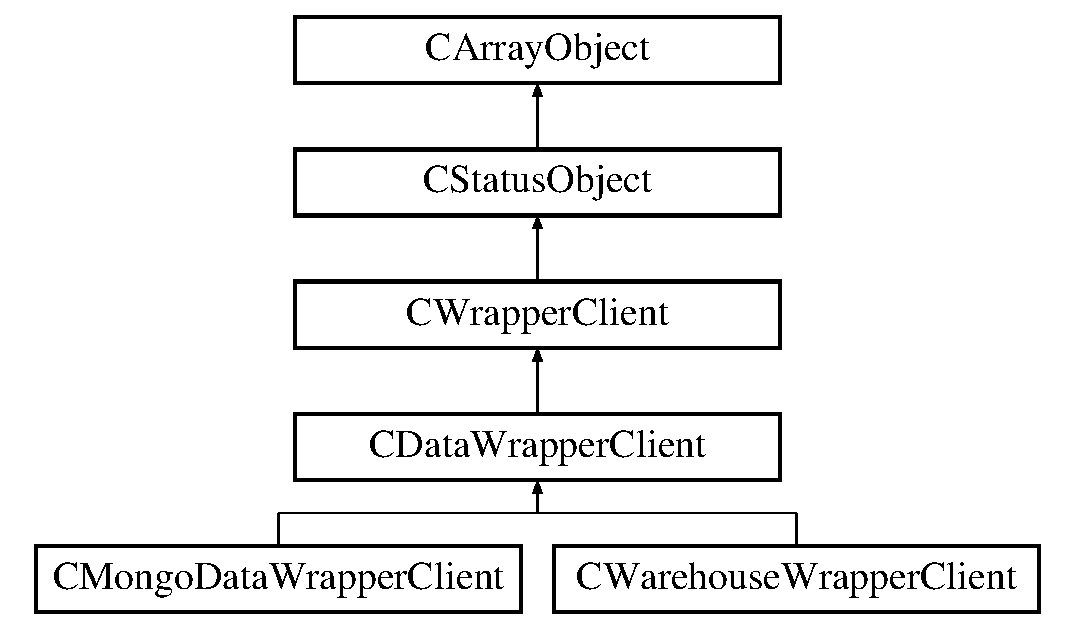
\includegraphics[height=5.000000cm]{class_c_wrapper_client}
\end{center}
\end{figure}
\subsection*{Public Member Functions}
\begin{DoxyCompactItemize}
\item 
\hyperlink{class_c_wrapper_client_a79e4150b435f337facf72119c289efbd}{\-\_\-\-\_\-construct} (\$the\-Data=N\-U\-L\-L)
\item 
\hyperlink{class_c_wrapper_client_ad8b041a29054f790a0a4fd65745da0ee}{Url} (\$the\-Value=N\-U\-L\-L, \$get\-Old=F\-A\-L\-S\-E)
\item 
\hyperlink{class_c_wrapper_client_ae378229fd57b051ddf0e0a7abf599641}{Operation} (\$the\-Value=N\-U\-L\-L, \$get\-Old=F\-A\-L\-S\-E)
\item 
\hyperlink{class_c_wrapper_client_aeea011893f53a7df495f23e199cbc28b}{Format} (\$the\-Value=N\-U\-L\-L, \$get\-Old=F\-A\-L\-S\-E)
\item 
\hyperlink{class_c_wrapper_client_ac87e4af5c32d735f192c8041e83b3ce3}{Stamp} (\$the\-Value=N\-U\-L\-L, \$get\-Old=F\-A\-L\-S\-E)
\item 
\hyperlink{class_c_wrapper_client_a844a2e677c1e0fb0855255cb02b86be4}{Log\-Request} (\$the\-Value=N\-U\-L\-L, \$get\-Old=F\-A\-L\-S\-E)
\item 
\hyperlink{class_c_wrapper_client_a2020117737285ff3c2c3f0fae01136ff}{Log\-Trace} (\$the\-Value=N\-U\-L\-L, \$get\-Old=F\-A\-L\-S\-E)
\item 
\hyperlink{class_c_wrapper_client_ac37ea353c211b696d11e103a069e8633}{offset\-Set} (\$the\-Offset, \$the\-Value)
\item 
\hyperlink{class_c_wrapper_client_af4a349c007923b1229f3099592660d97}{offset\-Unset} (\$the\-Offset)
\item 
\hyperlink{class_c_wrapper_client_a49dde8406fa42352792b99163f04c8c7}{Execute} (\$the\-Mode= 'P\-O\-S\-T')
\end{DoxyCompactItemize}
\subsection*{Static Public Member Functions}
\begin{DoxyCompactItemize}
\item 
static \hyperlink{class_c_wrapper_client_ac82b7d383afcfaa312f6db5eee1db4e2}{Request} (\$the\-Url, \$the\-Params=N\-U\-L\-L, \$the\-Mode= 'P\-O\-S\-T', \$the\-Format=k\-T\-Y\-P\-E\-\_\-\-J\-S\-O\-N)
\end{DoxyCompactItemize}
\subsection*{Additional Inherited Members}


\subsection{Constructor \& Destructor Documentation}
\hypertarget{class_c_wrapper_client_a79e4150b435f337facf72119c289efbd}{\index{C\-Wrapper\-Client@{C\-Wrapper\-Client}!\-\_\-\-\_\-construct@{\-\_\-\-\_\-construct}}
\index{\-\_\-\-\_\-construct@{\-\_\-\-\_\-construct}!CWrapperClient@{C\-Wrapper\-Client}}
\subsubsection[{\-\_\-\-\_\-construct}]{\setlength{\rightskip}{0pt plus 5cm}C\-Wrapper\-Client\-::\-\_\-\-\_\-construct (
\begin{DoxyParamCaption}
\item[{}]{\$the\-Data = {\ttfamily NULL}}
\end{DoxyParamCaption}
)}}\label{class_c_wrapper_client_a79e4150b435f337facf72119c289efbd}
Instantiate class.

The constructor will initialise the object depending on the provided parameter\-:


\begin{DoxyItemize}
\item {\itshape N\-U\-L\-L}\-: An empty object. 
\item {\itshape array}\-: The array elements will become the object properties. 
\item {\itshape string}\-: Any other value will be converted to string and will represent the web-\/service U\-R\-L. 
\end{DoxyItemize}


\begin{DoxyParams}[1]{Parameters}
string & {\em \$the\-Data} & Web-\/service U\-R\-L or object data.\\
\hline
\end{DoxyParams}
public 

\subsection{Member Function Documentation}
\hypertarget{class_c_wrapper_client_a49dde8406fa42352792b99163f04c8c7}{\index{C\-Wrapper\-Client@{C\-Wrapper\-Client}!Execute@{Execute}}
\index{Execute@{Execute}!CWrapperClient@{C\-Wrapper\-Client}}
\subsubsection[{Execute}]{\setlength{\rightskip}{0pt plus 5cm}C\-Wrapper\-Client\-::\-Execute (
\begin{DoxyParamCaption}
\item[{}]{\$the\-Mode = {\ttfamily 'POST'}}
\end{DoxyParamCaption}
)}}\label{class_c_wrapper_client_a49dde8406fa42352792b99163f04c8c7}
Send an H\-T\-T\-P request.

This method can be used to sent an {\itshape H\-T\-T\-P} request using the current contents of the object and return a response.


\begin{DoxyParams}[1]{Parameters}
string & {\em \$the\-Mode} & Request mode, P\-O\-S\-T or G\-E\-T\\
\hline
\end{DoxyParams}
public \begin{DoxyReturn}{Returns}
mixed
\end{DoxyReturn}

\begin{DoxyExceptions}{Exceptions}
{\em \{@link} & \hyperlink{class_c_exception}{C\-Exception} \hyperlink{class_c_exception}{C\-Exception}\} \\
\hline
\end{DoxyExceptions}
\hypertarget{class_c_wrapper_client_aeea011893f53a7df495f23e199cbc28b}{\index{C\-Wrapper\-Client@{C\-Wrapper\-Client}!Format@{Format}}
\index{Format@{Format}!CWrapperClient@{C\-Wrapper\-Client}}
\subsubsection[{Format}]{\setlength{\rightskip}{0pt plus 5cm}C\-Wrapper\-Client\-::\-Format (
\begin{DoxyParamCaption}
\item[{}]{\$the\-Value = {\ttfamily NULL}, }
\item[{}]{\$get\-Old = {\ttfamily FALSE}}
\end{DoxyParamCaption}
)}}\label{class_c_wrapper_client_aeea011893f53a7df495f23e199cbc28b}
Manage format.

This method can be used to manage the \hyperlink{}{format} in which both the parameters are sent and the response is returned from the web-\/service. It accepts a parameter which represents either the web-\/service format code or this method operation, depending on its value\-:


\begin{DoxyItemize}
\item {\itshape N\-U\-L\-L}\-: Return the current value. 
\item {\itshape F\-A\-L\-S\-E}\-: Delete the current value. 
\item {\itshape other}\-: Set the value with the provided parameter. 
\end{DoxyItemize}

The second parameter is a boolean which if {\itshape T\-R\-U\-E} will return the {\itshape old} value when replacing values; if {\itshape F\-A\-L\-S\-E}, it will return the currently set value.

This method will check whether the provided format is supported, if this is not the case, it will raise an exception. Derived classes should first check their specific operations, if not matched, they should pass the parameter to the parent method. In this class we support the following operations\-:


\begin{DoxyItemize}
\item {\itshape \hyperlink{}{k\-T\-Y\-P\-E\-\_\-\-P\-H\-P}}\-: Parameters and response will be serialized. 
\item {\itshape \hyperlink{}{k\-T\-Y\-P\-E\-\_\-\-X\-M\-L}}\-: Parameters and response will be encoded in X\-M\-L. 
\item {\itshape \hyperlink{}{k\-T\-Y\-P\-E\-\_\-\-J\-S\-O\-N}}\-: Parameters and response will be encoded in J\-S\-O\-N. 
\item {\itshape \hyperlink{}{k\-T\-Y\-P\-E\-\_\-\-M\-E\-T\-A}}\-: This data type can be used to return service metadata, the \hyperlink{class_c_wrapper_client_a49dde8406fa42352792b99163f04c8c7}{request} will return headers metadata for troubleshooting, rather than the response from the web-\/service. 
\end{DoxyItemize}


\begin{DoxyParams}[1]{Parameters}
string & {\em \$the\-Value} & Value or operation. \\
\hline
boolean & {\em \$get\-Old} & T\-R\-U\-E get old value.\\
\hline
\end{DoxyParams}
public \begin{DoxyReturn}{Returns}
mixed
\end{DoxyReturn}

\begin{DoxyExceptions}{Exceptions}
{\em \{@link} & \hyperlink{class_c_exception}{C\-Exception} \hyperlink{class_c_exception}{C\-Exception}\}\\
\hline
\end{DoxyExceptions}
\hyperlink{class_c_attribute_a9d231a47718719fcd6c33f3d0ac91675}{C\-Attribute\-::\-Manage\-Offset()}

\begin{DoxySeeAlso}{See Also}
k\-A\-P\-I\-\_\-\-F\-O\-R\-M\-A\-T 

k\-A\-P\-I\-\_\-\-O\-P\-\_\-\-H\-E\-L\-P k\-A\-P\-I\-\_\-\-O\-P\-\_\-\-P\-I\-N\-G 
\end{DoxySeeAlso}
\hypertarget{class_c_wrapper_client_a844a2e677c1e0fb0855255cb02b86be4}{\index{C\-Wrapper\-Client@{C\-Wrapper\-Client}!Log\-Request@{Log\-Request}}
\index{Log\-Request@{Log\-Request}!CWrapperClient@{C\-Wrapper\-Client}}
\subsubsection[{Log\-Request}]{\setlength{\rightskip}{0pt plus 5cm}C\-Wrapper\-Client\-::\-Log\-Request (
\begin{DoxyParamCaption}
\item[{}]{\$the\-Value = {\ttfamily NULL}, }
\item[{}]{\$get\-Old = {\ttfamily FALSE}}
\end{DoxyParamCaption}
)}}\label{class_c_wrapper_client_a844a2e677c1e0fb0855255cb02b86be4}
Log request switch.

This method can be used to turn on or off the request section in the web-\/service response, the method accepts a single parameter that if resolves to {\itshape T\-R\-U\-E} it will turn on this option, if not it will turn it off.

The second parameter is a boolean which if {\itshape T\-R\-U\-E} will return the {\itshape old} value when replacing values; if {\itshape F\-A\-L\-S\-E}, it will return the currently set value.


\begin{DoxyParams}[1]{Parameters}
boolean & {\em \$the\-Value} & T\-R\-U\-E or F\-A\-L\-S\-E. \\
\hline
boolean & {\em \$get\-Old} & T\-R\-U\-E get old value.\\
\hline
\end{DoxyParams}
public \begin{DoxyReturn}{Returns}
mixed
\end{DoxyReturn}
\hyperlink{class_c_attribute_a9d231a47718719fcd6c33f3d0ac91675}{C\-Attribute\-::\-Manage\-Offset()}

\begin{DoxySeeAlso}{See Also}
k\-A\-P\-I\-\_\-\-O\-P\-T\-\_\-\-L\-O\-G\-\_\-\-R\-E\-Q\-U\-E\-S\-T 
\end{DoxySeeAlso}
\hypertarget{class_c_wrapper_client_a2020117737285ff3c2c3f0fae01136ff}{\index{C\-Wrapper\-Client@{C\-Wrapper\-Client}!Log\-Trace@{Log\-Trace}}
\index{Log\-Trace@{Log\-Trace}!CWrapperClient@{C\-Wrapper\-Client}}
\subsubsection[{Log\-Trace}]{\setlength{\rightskip}{0pt plus 5cm}C\-Wrapper\-Client\-::\-Log\-Trace (
\begin{DoxyParamCaption}
\item[{}]{\$the\-Value = {\ttfamily NULL}, }
\item[{}]{\$get\-Old = {\ttfamily FALSE}}
\end{DoxyParamCaption}
)}}\label{class_c_wrapper_client_a2020117737285ff3c2c3f0fae01136ff}
Log trace switch.

This method can be used to turn on or off the trace in the event an exception is raised, the method accepts a single parameter that if resolves to {\itshape T\-R\-U\-E} it will turn on this option, if not it will turn it off.

The second parameter is a boolean which if {\itshape T\-R\-U\-E} will return the {\itshape old} value when replacing values; if {\itshape F\-A\-L\-S\-E}, it will return the currently set value.


\begin{DoxyParams}[1]{Parameters}
boolean & {\em \$the\-Value} & T\-R\-U\-E or F\-A\-L\-S\-E. \\
\hline
boolean & {\em \$get\-Old} & T\-R\-U\-E get old value.\\
\hline
\end{DoxyParams}
public \begin{DoxyReturn}{Returns}
mixed
\end{DoxyReturn}
\hyperlink{class_c_attribute_a9d231a47718719fcd6c33f3d0ac91675}{C\-Attribute\-::\-Manage\-Offset()}

\begin{DoxySeeAlso}{See Also}
k\-A\-P\-I\-\_\-\-O\-P\-T\-\_\-\-L\-O\-G\-\_\-\-T\-R\-A\-C\-E 
\end{DoxySeeAlso}
\hypertarget{class_c_wrapper_client_ac37ea353c211b696d11e103a069e8633}{\index{C\-Wrapper\-Client@{C\-Wrapper\-Client}!offset\-Set@{offset\-Set}}
\index{offset\-Set@{offset\-Set}!CWrapperClient@{C\-Wrapper\-Client}}
\subsubsection[{offset\-Set}]{\setlength{\rightskip}{0pt plus 5cm}C\-Wrapper\-Client\-::offset\-Set (
\begin{DoxyParamCaption}
\item[{}]{\$the\-Offset, }
\item[{}]{\$the\-Value}
\end{DoxyParamCaption}
)}}\label{class_c_wrapper_client_ac37ea353c211b696d11e103a069e8633}
Set a value for a given offset.

We overload this method to manage the \hyperlink{class_c_status_object_a8429102e4f52f7558649b64f4e673a69}{inited} \hyperlink{}{status}\-: this is set if \hyperlink{}{U\-R\-L}, \hyperlink{}{operation} and \hyperlink{}{format} are all set.


\begin{DoxyParams}[1]{Parameters}
string & {\em \$the\-Offset} & Offset. \\
\hline
string | N\-U\-L\-L & {\em \$the\-Value} & Value to set at offset.\\
\hline
\end{DoxyParams}
public 

Reimplemented from \hyperlink{class_c_status_object_a140ef140d4fa1c4a6180e843bd5ec969}{C\-Status\-Object}.

\hypertarget{class_c_wrapper_client_af4a349c007923b1229f3099592660d97}{\index{C\-Wrapper\-Client@{C\-Wrapper\-Client}!offset\-Unset@{offset\-Unset}}
\index{offset\-Unset@{offset\-Unset}!CWrapperClient@{C\-Wrapper\-Client}}
\subsubsection[{offset\-Unset}]{\setlength{\rightskip}{0pt plus 5cm}C\-Wrapper\-Client\-::offset\-Unset (
\begin{DoxyParamCaption}
\item[{}]{\$the\-Offset}
\end{DoxyParamCaption}
)}}\label{class_c_wrapper_client_af4a349c007923b1229f3099592660d97}
Reset a value for a given offset.

We overload this method to manage the \hyperlink{class_c_status_object_a8429102e4f52f7558649b64f4e673a69}{inited} \hyperlink{}{status}\-: this is set if \hyperlink{}{U\-R\-L}, \hyperlink{}{operation} and \hyperlink{}{format} are all set.


\begin{DoxyParams}[1]{Parameters}
string & {\em \$the\-Offset} & Offset.\\
\hline
\end{DoxyParams}
public 

Reimplemented from \hyperlink{class_c_status_object_ae733db1bbfffcbe894ea405765ab4150}{C\-Status\-Object}.

\hypertarget{class_c_wrapper_client_ae378229fd57b051ddf0e0a7abf599641}{\index{C\-Wrapper\-Client@{C\-Wrapper\-Client}!Operation@{Operation}}
\index{Operation@{Operation}!CWrapperClient@{C\-Wrapper\-Client}}
\subsubsection[{Operation}]{\setlength{\rightskip}{0pt plus 5cm}C\-Wrapper\-Client\-::\-Operation (
\begin{DoxyParamCaption}
\item[{}]{\$the\-Value = {\ttfamily NULL}, }
\item[{}]{\$get\-Old = {\ttfamily FALSE}}
\end{DoxyParamCaption}
)}}\label{class_c_wrapper_client_ae378229fd57b051ddf0e0a7abf599641}
Manage operation.

This method can be used to manage the \hyperlink{}{operation}, it accepts a parameter which represents either the web-\/service operation code or this method operation, depending on its value\-:


\begin{DoxyItemize}
\item {\itshape N\-U\-L\-L}\-: Return the current value. 
\item {\itshape F\-A\-L\-S\-E}\-: Delete the current value. 
\item {\itshape other}\-: Set the value with the provided parameter. 
\end{DoxyItemize}

The second parameter is a boolean which if {\itshape T\-R\-U\-E} will return the {\itshape old} value when replacing values; if {\itshape F\-A\-L\-S\-E}, it will return the currently set value.

This method will check whether the provided operation is supported, if this is not the case, it will raise an exception. Derived classes should first check their specific operations, if not matched, they should pass the parameter to the parent method. In this class we support the following operations\-:


\begin{DoxyItemize}
\item {\itshape \hyperlink{}{k\-A\-P\-I\-\_\-\-O\-P\-\_\-\-H\-E\-L\-P}}\-: H\-E\-L\-P web-\/service operation, which returns the list of supported operations and options. 
\item {\itshape \hyperlink{}{k\-A\-P\-I\-\_\-\-O\-P\-\_\-\-P\-I\-N\-G}}\-: P\-I\-N\-G web-\/service operation, which returns a status response. 
\end{DoxyItemize}


\begin{DoxyParams}[1]{Parameters}
string & {\em \$the\-Value} & Value or operation. \\
\hline
boolean & {\em \$get\-Old} & T\-R\-U\-E get old value.\\
\hline
\end{DoxyParams}
public \begin{DoxyReturn}{Returns}
mixed
\end{DoxyReturn}

\begin{DoxyExceptions}{Exceptions}
{\em \{@link} & \hyperlink{class_c_exception}{C\-Exception} \hyperlink{class_c_exception}{C\-Exception}\}\\
\hline
\end{DoxyExceptions}
\hyperlink{class_c_attribute_a9d231a47718719fcd6c33f3d0ac91675}{C\-Attribute\-::\-Manage\-Offset()}

\begin{DoxySeeAlso}{See Also}
k\-A\-P\-I\-\_\-\-O\-P\-E\-R\-A\-T\-I\-O\-N 

k\-A\-P\-I\-\_\-\-O\-P\-\_\-\-H\-E\-L\-P k\-A\-P\-I\-\_\-\-O\-P\-\_\-\-P\-I\-N\-G 
\end{DoxySeeAlso}


Reimplemented in \hyperlink{class_c_data_wrapper_client_ae7cad4809c20d8f2871cfe00da909d67}{C\-Data\-Wrapper\-Client}, \hyperlink{class_c_mongo_data_wrapper_client_a730c4fe3a66ad8a5aa42e44f669632ac}{C\-Mongo\-Data\-Wrapper\-Client}, and \hyperlink{class_c_warehouse_wrapper_client_a099ef5aef1883aa5b394c7086a818496}{C\-Warehouse\-Wrapper\-Client}.

\hypertarget{class_c_wrapper_client_ac82b7d383afcfaa312f6db5eee1db4e2}{\index{C\-Wrapper\-Client@{C\-Wrapper\-Client}!Request@{Request}}
\index{Request@{Request}!CWrapperClient@{C\-Wrapper\-Client}}
\subsubsection[{Request}]{\setlength{\rightskip}{0pt plus 5cm}static C\-Wrapper\-Client\-::\-Request (
\begin{DoxyParamCaption}
\item[{}]{\$the\-Url, }
\item[{}]{\$the\-Params = {\ttfamily NULL}, }
\item[{}]{\$the\-Mode = {\ttfamily 'POST'}, }
\item[{}]{\$the\-Format = {\ttfamily kTYPE\-\_\-JSON}}
\end{DoxyParamCaption}
)\hspace{0.3cm}{\ttfamily [static]}}}\label{class_c_wrapper_client_ac82b7d383afcfaa312f6db5eee1db4e2}
Send a H\-T\-T\-P request.

This method can be used to sent an {\itshape H\-T\-T\-P} request via {\itshape G\-E\-T} or {\itshape P\-O\-S\-T}.

The method accepts the following parameters\-:


\begin{DoxyItemize}
\item {\bfseries \$the\-Url}\-: The request U\-R\-L. 
\item {\bfseries \$the\-Params}\-: An array of key/value parameters for the request. 
\item {\bfseries \$the\-Mode}\-: The request mode\-: 
\begin{DoxyItemize}
\item {\itshape G\-E\-T}\-: G\-E\-T, default. 
\item {\itshape P\-O\-S\-T}\-: P\-O\-S\-T. 
\end{DoxyItemize}
\item {\bfseries \$the\-Format}\-: The request format\-: 
\begin{DoxyItemize}
\item {\itshape \hyperlink{}{k\-T\-Y\-P\-E\-\_\-\-X\-M\-L}}\-: X\-M\-L. 
\item {\itshape \hyperlink{}{k\-T\-Y\-P\-E\-\_\-\-P\-H\-P}}\-: P\-H\-P. 
\item {\itshape \hyperlink{}{k\-T\-Y\-P\-E\-\_\-\-J\-S\-O\-N}}\-: J\-S\-O\-N. 
\item {\itshape \hyperlink{}{k\-T\-Y\-P\-E\-\_\-\-M\-E\-T\-A}}\-: Metadata\-: if you provide this format, the method will return the metadata of the operation for troubleshooting purposes. 
\end{DoxyItemize}
\end{DoxyItemize}


\begin{DoxyParams}[1]{Parameters}
string & {\em \$the\-Url} & Request U\-R\-L. \\
\hline
mixed & {\em \$the\-Params} & Request parameters. \\
\hline
string & {\em \$the\-Mode} & Request mode. \\
\hline
string & {\em \$the\-Format} & Response format.\\
\hline
\end{DoxyParams}
\begin{DoxyReturn}{Returns}
mixed
\end{DoxyReturn}

\begin{DoxyExceptions}{Exceptions}
{\em \{@link} & \hyperlink{class_c_exception}{C\-Exception} \hyperlink{class_c_exception}{C\-Exception}\} \\
\hline
\end{DoxyExceptions}
\hypertarget{class_c_wrapper_client_ac87e4af5c32d735f192c8041e83b3ce3}{\index{C\-Wrapper\-Client@{C\-Wrapper\-Client}!Stamp@{Stamp}}
\index{Stamp@{Stamp}!CWrapperClient@{C\-Wrapper\-Client}}
\subsubsection[{Stamp}]{\setlength{\rightskip}{0pt plus 5cm}C\-Wrapper\-Client\-::\-Stamp (
\begin{DoxyParamCaption}
\item[{}]{\$the\-Value = {\ttfamily NULL}, }
\item[{}]{\$get\-Old = {\ttfamily FALSE}}
\end{DoxyParamCaption}
)}}\label{class_c_wrapper_client_ac87e4af5c32d735f192c8041e83b3ce3}
Time-\/stamp switch.

This method can be used to turn on or off the time-\/stamp section in the web-\/service response, the method accepts a single parameter that if resolves to {\itshape T\-R\-U\-E} it will turn on this option, if not it will turn it off.

The second parameter is a boolean which if {\itshape T\-R\-U\-E} will return the {\itshape old} value when replacing values; if {\itshape F\-A\-L\-S\-E}, it will return the currently set value.


\begin{DoxyParams}[1]{Parameters}
boolean & {\em \$the\-Value} & T\-R\-U\-E or F\-A\-L\-S\-E. \\
\hline
boolean & {\em \$get\-Old} & T\-R\-U\-E get old value.\\
\hline
\end{DoxyParams}
public \begin{DoxyReturn}{Returns}
mixed
\end{DoxyReturn}
\hyperlink{class_c_attribute_a9d231a47718719fcd6c33f3d0ac91675}{C\-Attribute\-::\-Manage\-Offset()}

\begin{DoxySeeAlso}{See Also}
k\-A\-P\-I\-\_\-\-R\-E\-Q\-\_\-\-S\-T\-A\-M\-P 
\end{DoxySeeAlso}
\hypertarget{class_c_wrapper_client_ad8b041a29054f790a0a4fd65745da0ee}{\index{C\-Wrapper\-Client@{C\-Wrapper\-Client}!Url@{Url}}
\index{Url@{Url}!CWrapperClient@{C\-Wrapper\-Client}}
\subsubsection[{Url}]{\setlength{\rightskip}{0pt plus 5cm}C\-Wrapper\-Client\-::\-Url (
\begin{DoxyParamCaption}
\item[{}]{\$the\-Value = {\ttfamily NULL}, }
\item[{}]{\$get\-Old = {\ttfamily FALSE}}
\end{DoxyParamCaption}
)}}\label{class_c_wrapper_client_ad8b041a29054f790a0a4fd65745da0ee}
Manage U\-R\-L.

This method can be used to manage the \hyperlink{}{U\-R\-L}, it accepts a parameter which represents either the U\-R\-L or the requested operation, depending on its value\-:


\begin{DoxyItemize}
\item {\itshape N\-U\-L\-L}\-: Return the current value. 
\item {\itshape F\-A\-L\-S\-E}\-: Delete the current value. 
\item {\itshape other}\-: Set the value with the provided parameter. 
\end{DoxyItemize}

The second parameter is a boolean which if {\itshape T\-R\-U\-E} will return the {\itshape old} value when replacing values; if {\itshape F\-A\-L\-S\-E}, it will return the currently set value.


\begin{DoxyParams}[1]{Parameters}
string & {\em \$the\-Value} & Value or operation. \\
\hline
boolean & {\em \$get\-Old} & T\-R\-U\-E get old value.\\
\hline
\end{DoxyParams}
public \begin{DoxyReturn}{Returns}
mixed
\end{DoxyReturn}
\hyperlink{class_c_attribute_a9d231a47718719fcd6c33f3d0ac91675}{C\-Attribute\-::\-Manage\-Offset()}

\begin{DoxySeeAlso}{See Also}
k\-O\-F\-F\-S\-E\-T\-\_\-\-U\-R\-L 
\end{DoxySeeAlso}


The documentation for this class was generated from the following file\-:\begin{DoxyCompactItemize}
\item 
/\-Library/\-Web\-Server/\-Library/wrapper/classes/C\-Wrapper\-Client.\-php\end{DoxyCompactItemize}

\printindex
\end{document}
